\batchmode
\makeatletter
\def\input@path{{/Users/sergei.winitzki/Code/talks/ftt-fp/}}
\makeatother
\documentclass[10pt,american,english,numbers=noenddot,index=totoc,bibliography=totoc,fontsize=10pt,utf8]{scrbook}
\usepackage{amsmath}
\usepackage{mathpazo}
\usepackage{helvet}
\renewcommand{\ttdefault}{cmtt}
\usepackage{newtxmath}
\usepackage[T1]{fontenc}
\usepackage[latin9]{inputenc}
\usepackage[paperwidth=7in,paperheight=9in]{geometry}
\setcounter{secnumdepth}{3}
\usepackage{color}
\usepackage{babel}
\usepackage{verbatim}
\usepackage{makeidx}
\makeindex
\usepackage{graphicx}
\usepackage{wasysym}
\usepackage[all]{xy}
\usepackage[unicode=true,
 bookmarks=true,bookmarksnumbered=true,bookmarksopen=true,bookmarksopenlevel=2,
 breaklinks=true,pdfborder={0 0 0},pdfborderstyle={},backref=page,colorlinks=true]
 {hyperref}
\hypersetup{pdftitle={Science of functional programming},
 pdfauthor={Sergei Winitzki},
 pdfsubject={Functional programming},
 pdfkeywords={Functional programming, Type theory, Category theory, Formal logic, Programming languages},
 linkcolor=blue}

\makeatletter

%%%%%%%%%%%%%%%%%%%%%%%%%%%%%% LyX specific LaTeX commands.
\newcommand{\noun}[1]{\textsc{#1}}
%% Because html converters don't know tabularnewline
\providecommand{\tabularnewline}{\\}

%%%%%%%%%%%%%%%%%%%%%%%%%%%%%% Textclass specific LaTeX commands.
\newenvironment{lyxcode}
	{\par\begin{list}{}{
		\setlength{\rightmargin}{\leftmargin}
		\setlength{\listparindent}{0pt}% needed for AMS classes
		\raggedright
		\setlength{\itemsep}{0pt}
		\setlength{\parsep}{0pt}
		\normalfont\ttfamily}%
	 \item[]}
	{\end{list}}

%%%%%%%%%%%%%%%%%%%%%%%%%%%%%% User specified LaTeX commands.
\usepackage[all]{xy} % xypic

% Fix the numbering of exercises: subsubsections appear as paragraphs but are numbered.
\usepackage{titlesec}
\titleformat{\subsubsection}[runin]{\normalfont\normalsize\bfseries}{}{0pt}{}

% Scala syntax highlighting. See https://tex.stackexchange.com/questions/202479/unable-to-define-scala-language-with-listings
%\usepackage[T1]{fontenc}
%\usepackage[utf8]{inputenc}
%\usepackage{beramono}
%\usepackage{listings}
\usepackage{xcolor}

\definecolor{scalakeyword}{rgb}{0.16,0.07,0.5}
\definecolor{dkgreen}{rgb}{0,0.6,0}
\definecolor{gray}{rgb}{0.5,0.5,0.5}
\definecolor{mauve}{rgb}{0.58,0,0.82}
\definecolor{aqua}{rgb}{0.9,0.96,0.999}
\definecolor{scalatype}{rgb}{0.2,0.3,0.2}

%\lstdefinestyle{myScalastyle}{
%  language=scala, % This should be defined first!!! Otherwise it overrides all customization via morekeywords / otherkeywords.
%  otherkeywords={{=,=>,<-,<\%,<:,>:,\#,@,*,+,-,/,::,:,[,]}},
%  frame=tb,
%  aboveskip=2mm,
%  belowskip=2mm,
%  showstringspaces=false,
%  columns=flexible,
%  basicstyle={\small\ttfamily},
%  extendedchars=true,
%  %numbers=none,
%  numberstyle=\tiny\color{gray},
%  keywordstyle=\color{blue},
%  commentstyle=\color{dkgreen},
%  stringstyle=\color{mauve},
%  frame=single,
%  framerule=0.01mm,
%  breaklines=true,
%  breakatwhitespace=true,
%  tabsize=3,
%  framexleftmargin=4mm, framexrightmargin=4mm,
%  xleftmargin=4mm, xrightmargin=4mm, % Making these margins the same has a good effect.
%  framextopmargin=0.5mm, framexbottommargin=.5mm,
%  fillcolor=\color{aqua},
%  rulecolor=\color{aqua},
%  rulesepcolor=\color{aqua},
%  backgroundcolor=\color{aqua},
%  mathescape=true,
%}

% Example usage: \begin{lstlisting}[style=myScalastyle]  object blah \end{lstlisting}
%\newenvironment{scala}{\begin{lstlisting}[style=myScalastyle]}{\end{lstlisting}}
%\lstnewenvironment{scala}{\lstset{style=myScalastyle}}{}

\usepackage[nocenter]{qtree} % simple tree drawing
\usepackage{relsize} % make math symbols larger or smaller
\usepackage{relsize} % make math symbols larger or smaller
\usepackage{stmaryrd} % some extra symbols such as \fatsemi
% Note: using \bef inside a \text{} will cause a LaTeX error!
\newcommand{\bef}{\hspace{0.5pt}\ensuremath\mathsmaller{\fatsemi}\hspace{1.5pt}}
% this is ugly:
%\newcommand{\bef}{\hspace{1.0pt}\ensuremath\raisebox{2pt}{$\mathsmaller{\mathsmaller{\circ}}$}\hspace{-2.9pt},}
%\makeatletter
% Macros to assist LyX with XYpic when using scaling.
\newcommand{\xyScaleX}[1]{%
\makeatletter
\xydef@\xymatrixcolsep@{#1}
\makeatother
} % end of \xyScaleX
\makeatletter
\newcommand{\xyScaleY}[1]{%
\makeatletter
\xydef@\xymatrixrowsep@{#1}
\makeatother
} % end of \xyScaleY

\makeatother

\usepackage{listings}
\lstset{language=Scala,
morekeywords={{scala}},
otherkeywords={=,=>,<-,<\%,<:,>:,\#,@,:,[,],.,???},
keywordstyle={\color{scalakeyword}},
morekeywords={[2]{String,Int,Char,Boolean,Double,Float,Long,Seq,Map,List,Option,Either,Future,Vector,IndexedSeq,Try,true,false,None,Some,Left,Right,Nothing,Any,Array,Unit}},
keywordstyle={[2]{\color{scalatype}}},
frame=tb,
aboveskip=2mm,
belowskip=2mm,
showstringspaces=false,
columns=fullflexible,
keepspaces=true,
basicstyle={\small\ttfamily},
extendedchars=true,
numbers=none,
numberstyle={\tiny\color{gray}},
commentstyle={\color{dkgreen}},
stringstyle={\color{mauve}},
frame=single,
framerule={0.01mm},
breaklines=true,
breakatwhitespace=true,
tabsize=3,
framexleftmargin=4mm,
framexrightmargin=4mm,
xleftmargin=4mm,
xrightmargin=4mm,
framextopmargin={0.5mm},
framexbottommargin={.5mm},
fillcolor={\color{aqua}},
rulecolor={\color{aqua}},
rulesepcolor={\color{aqua}},
backgroundcolor={\color{aqua}},
mathescape=true}
\addto\captionsamerican{\renewcommand{\lstlistingname}{Listing}}
\addto\captionsenglish{\renewcommand{\lstlistingname}{Listing}}
\renewcommand{\lstlistingname}{Listing}

\begin{document}

\title{The Science of Functional Programming}

\subtitle{Applied Functional Type Theory, with Examples in Scala}

\author{by Sergei Winitzki, Ph.D.}

\date{draft version 0.2, \today}

\publishers{Published by \textbf{\href{http://lulu.com}{lulu.com}} 2019}

\uppertitleback{Copyright \copyright\  2018-2019 by Sergei Winitzki\\
Published and printed by~ \textbf{\href{http://lulu.com}{lulu.com}}\\
Permission is granted to copy, distribute and/or modify this document
under the terms of the GNU Free Documentation License, Version 1.2
or any later version published by the Free Software Foundation; with
no Invariant Sections, no Front-Cover Texts, and no Back-Cover Texts.
A copy of the license is included in the section entitled \textquotedblleft GNU
Free Documentation License\textquotedblright{} (Appendix~\ref{sec:GFDL}).\\
ISBN XXXXXX}

\lowertitleback{This book presents the theoretical knowledge that helps to write
code in the functional programming paradigm. Detailed explanations
and derivations are logically developed and accompanied by worked
examples tested in the Scala interpreter. Exercises with solutions
are provided. Readers need to have a working knowledge of basic Scala
(e.g.\ be able to write code that reads a small text file and prints
all word counts, sorted in descending order by count). Readers should
also have a basic command of school-level mathematics; for example,
be able to simplify the expressions such as $\frac{1}{x-2}-\frac{1}{x+2}$
and $\frac{d}{dx}\left(\left(x+1\right)e^{-x}\right)$.}

\maketitle
\tableofcontents{}

\selectlanguage{american}%
\mainmatter\pagenumbering{arabic}
\selectlanguage{english}%

\chapter{Values, types, expressions, functions\label{chap:1-Values,-types,-expressions,}}

\section{Translating mathematics into code}

\subsection{First examples}

We begin by writing Scala code for some computational tasks.

\paragraph{Factorial of 10}

Find the product of integers from $1$ to $10$ (the \textbf{factorial\index{factorial}}
of 10).

First, we write a mathematical formula for the result:
\[
\prod_{k=1}^{10}k\quad.
\]
We can then write Scala code in a way that resembles this formula:
\begin{lstlisting}
scala> (1 to 10).product
res0: Int = 3628800
\end{lstlisting}

The Scala interpreter indicates that the result is the value $3628800$
of type \lstinline!Int!. If we need to define a name for this value
(e.g.\ to use it later), we use the ``\lstinline!val!'' syntax
and write
\begin{lstlisting}
scala> val fac10 = (1 to 10).product
fac10: Int = 3628800

scala> fac10 == 3628800
res1: Boolean = true
\end{lstlisting}

The code \texttt{}\lstinline!(1 to 10).product! is an \textbf{expression}\index{expression},
which means two things: (1) it can be computed (e.g.~with the Scala
interpreter) and yields a value, and (2) the code can be inserted
anywhere as part of a larger expression; for example, we could write
\begin{lstlisting}
scala> 100 + (1 to 10).product + 100
res0: Int = 3629000
\end{lstlisting}


\paragraph{Factorial as a function}

Define a function that takes an integer $n$ and computes the factorial
of $n$.

A mathematical formula for this function can be written as
\[
f\left(n\right)=\prod_{k=1}^{n}k\quad.
\]
The corresponding Scala code is
\begin{lstlisting}
def f(n:Int) = (1 to n).product
\end{lstlisting}

In Scala's \texttt{}\lstinline!def! syntax, we need to specify the
type of a function's argument; in this case, we write \lstinline!n:Int!.
In the usual mathematical notation, types of arguments are either
not written at all, or written separately from the formula:
\[
f(n)=\prod_{k=1}^{n}k,\quad\forall n\in\mathbb{N}\quad.
\]
This indicates that $n$ must be from the set of non-negative integers
(denoted by $\mathbb{N}$ in mathematics). This is quite similar to
specifying the type \texttt{}\lstinline!Int! in the Scala code.
So, the argument's type in the code specifies the \emph{domain} of
a function.

Having defined the function \texttt{f}, we can now apply it to an
integer argument: 
\begin{lstlisting}
scala> f(10)
res6: Int = 3628800
\end{lstlisting}
It is an error to apply \texttt{f} to a non-integer value, e.g.\ to
a string:
\begin{lstlisting}
scala> f("abc")
<console>:13: error: type mismatch;
 found   : String("abc")
 required: Int
       f("abc")
         ^ 
\end{lstlisting}


\subsection{Nameless functions}

The formula and the code, as written above, both involve \emph{naming}
the function as ``$f$''. What if we do not need to name that function,
for instance, if $f$ is used only once? We could denote ``nameless''
mathematical functions like this: 
\[
x\Rightarrow\left(\text{some formula}\right)\quad.
\]
Then the mathematical notation for the nameless factorial function
is
\[
n\Rightarrow\prod_{k=1}^{n}k\quad.
\]
This reads as ``a function that maps $n$ to the product of all $k$
where $k$ goes from $1$ to $n$''. The Scala expression implementing
this mathematical formula is
\begin{lstlisting}
(n: Int) => (1 to n).product
\end{lstlisting}
This expression shows Scala's syntax for a nameless\index{nameless function}
function. Here, 
\begin{lstlisting}
n: Int
\end{lstlisting}
is the function's \textbf{argument}, while
\begin{lstlisting}
(1 to n).product
\end{lstlisting}
is the function's \textbf{body}. The double arrow symbol \lstinline!=>!
separates the argument from the body.\footnote{In Scala, the two ASCII characters \texttt{=>} and the single Unicode
character $\Rightarrow$ have the same meaning. I use the symbol $\Rightarrow$
in this book. However, when I write functional programming calculations
\emph{by hand}, I tend to write $\rightarrow$ instead of $\Rightarrow$
since it is faster. Several programming languages, such as OCaml and
Haskell, use the symbols \texttt{->} or the Unicode equivalent, $\rightarrow$,
for the function arrow.} 

Functions in Scala (whether named or nameless) are treated as values\index{function value},
which means that we can also define a Scala value \texttt{fac} as
\begin{lstlisting}
scala> val fac = (n: Int) => (1 to n).product
fac: Int => Int = <function1>
\end{lstlisting}
We see that the value \texttt{fac} has the type \lstinline!Int => Int!,
which means that the function takes an integer argument and returns
an integer result value. What is the value of the function \texttt{fac}
\emph{itself}? As we have just seen, the Scala interpreter prints
\lstinline!<function1>! as the ``value'' of \texttt{fac}. An alternative
Scala interpreter called \texttt{ammonite}\footnote{See \href{https://ammonite.io/}{https://ammonite.io/}}
prints something like this,
\begin{lstlisting}%
[mathescape=false]
scala@ val fac = (n: Int) => (1 to n).product
fac: Int => Int = ammonite.$sess.cmd0$$$Lambda$1675/2107543287@1e44b638
\end{lstlisting}
This seems to indicate some identifying number, or perhaps a memory
location.

I usually imagine that a function value represents a \emph{block of
compiled machine code}, \textemdash{} code that will actually run
and evaluate the function body when the function is applied.

Once defined, a function value can be applied to an argument:
\begin{lstlisting}
scala> fac(10)
res1: Int = 3628800
\end{lstlisting}

However, functions can be used without naming them. We can directly
apply a nameless factorial function to an integer argument \lstinline!10!
instead of writing \lstinline!fac(10)!:
\begin{lstlisting}
scala> ((n: Int) => (1 to n).product)(10)
res2: Int = 3628800
\end{lstlisting}
One would not often write code like this because there is no advantage
in creating a nameless function and then applying it right away to
an argument. We can evaluate the expression
\begin{lstlisting}
((n: Int) => (1 to n).product)(10)
\end{lstlisting}
 by substituting \lstinline!10! instead of \lstinline!n! in the
function body, which gives us
\begin{lstlisting}
(1 to 10).product
\end{lstlisting}

If a nameless function uses the argument several times, for example
\begin{lstlisting}
((n: Int) => n*n*n + n*n)(12345)
\end{lstlisting}
it is still better to substitute the argument and to eliminate the
nameless function. We could have written
\begin{lstlisting}
12345*12345*12345 + 12345*12345
\end{lstlisting}
but, of course, we want to avoid repeating the value \lstinline!12345!.
To achieve that, we may define \texttt{}\lstinline!n! as a value
in an \textbf{expression block\index{expression block}} like this:
\begin{lstlisting}
scala> { val n = 12345; n*n*n + n*n }
res3: Int = 322687002
\end{lstlisting}
Defined in this way, the value \lstinline!n! is visible only within
the expression block. Outside the block, another value named \lstinline!n!
could be defined completely independently of this \lstinline!n!.
For this reason, the definition of \lstinline!n! is called a \textbf{local}\index{local value}
value definition.

Nameless functions are most useful when they are themselves arguments
of other functions, as we will see next.

\paragraph{Checking integers for being prime}

Define a function that takes an integer $n$ and determines whether
$n$ is a prime number.

A simple mathematical formula for this function can be written as
\begin{equation}
\text{is\_prime}\left(n\right)=\forall k\in\left[2,n-1\right]\ :\ n\neq0\mod k\quad.\label{eq:is_prime_def}
\end{equation}
This formula has two clearly separated parts: first, a range of integers
from $2$ to $n-1$, and second, a requirement that all these integers
should satisfy a given condition, $n\neq0\mod k$.

This mathematical expression is translated into the Scala code as
\begin{lstlisting}
def is_prime(n: Int) =
  (2 to n-1).forall(k => n % k != 0)
\end{lstlisting}
In this code, the two parts of the mathematical formula are implemented
in a way that is closely similar to the mathematical notation, except
for the arrow after $k$.

We can now apply the function \texttt{is\_prime} to some integer values:
\begin{lstlisting}
scala> is_prime(12)
res3: Boolean = false

scala> is_prime(13)
res4: Boolean = true
\end{lstlisting}
As we can see from the output above, the function \texttt{is\_prime}
returns a value of type \lstinline!Boolean!. Therefore, the function
\texttt{is\_prime} has type \lstinline!Int => Boolean!.

A function that returns a \lstinline!Boolean! value is called a \textbf{predicate}\index{predicate}.

In Scala, it is optional\textemdash but strongly recommended\textemdash to
specify the return type of named functions. The required syntax looks
like this,
\begin{lstlisting}
def is_prime(n: Int): Boolean =
  (2 to n-1).forall(k => n % k != 0)
\end{lstlisting}

However, we do not need to specify the type \texttt{}\lstinline!Int!
for the argument \texttt{}\lstinline!k! of the nameless function
\lstinline*k => n % k != 0*. This is because the Scala compiler knows
that \texttt{}\lstinline!k! is going to iterate over the \emph{integer}
elements of the range \lstinline!(2 to n-1)!, which effectively forces
\texttt{}\lstinline!k! to be of type \lstinline!Int!.

\subsection{Nameless functions and bound variables}

The Scala code for \texttt{is\_prime} differs from the mathematical
formula\ (\ref{eq:is_prime_def}) in two ways.

One difference is that the interval $\left[2,n-1\right]$ comes first
in the Scala expression. To understand this, look at the ways Scala
allows programmers to define syntax.

The Scala syntax such as \texttt{}\lstinline!(2 to n-1).forall(k => ...)!
means to apply a function called \texttt{}\lstinline!forall! to
\emph{two} arguments: the first argument is the range \texttt{}\lstinline!(2 to n-1)!\texttt{,}
and the second argument is the nameless function \lstinline!(k => ...)!.
In Scala, the \textbf{infix} syntax\index{infix syntax} \lstinline!x.f(z)!,
or equivalently \lstinline!x f z!, means that a function \texttt{}\lstinline!f!
is applied to its \emph{two} arguments, \texttt{}\lstinline!x! and
\lstinline!z!. In the ordinary mathematical notation, this would
be $f(x,z)$. Infix notation is often easier to read and is also widely
used in mathematics, for instance when we write $x+y$ rather than
something like $plus(x,y)$.

A single-argument function could be also defined with infix notation,
and then the syntax is \lstinline!x.f!, as in the expression \texttt{}\lstinline!(1 to n).product!
we have seen before.

The infix methods \texttt{}\lstinline!.product! and \texttt{}\lstinline!.forall!
are already provided in the Scala standard library, so it is natural
to use them. If we want to avoid the infix syntax, we could define
a function \texttt{for\_all} with two arguments and write code like
this,

\begin{lstlisting}
for_all(2 to n-1, k => n % k != 0)
\end{lstlisting}
This would have brought the syntax somewhat closer to the formula\ (\ref{eq:is_prime_def}). 

However, there still remains the second difference: The symbol $k$
is used as an \emph{argument} of a nameless function \texttt{}\lstinline*(k => n % k != 0)*
in the Scala code, \textemdash{} while the mathematical notation,
such as 
\[
\forall k\in\left[2,n-1\right]\ :\ n\neq0\mod k\quad,
\]
does not seem to involve any nameless functions. Instead, the mathematical
formula defines the symbol $k$ that ``goes over a certain set,''
as we might say. The symbol $k$ is then used for writing the predicate
$n\neq0\mod k$. 

However, let us investigate the role of the symbol $k$ more closely. 

The symbol $k$ is a mathematical variable that is actually defined
\emph{only inside} the expression ``$\forall k:...$'' and makes
no sense outside that expression. This becomes clear by looking at
Eq.\ (\ref{eq:is_prime_def}): The variable $k$ is not present in
the left-hand side and could not possibly be used there. The name
``$k$'' is defined only in the right-hand side, where it is first
mentioned as the arbitrary element $k\in\left[2,n-1\right]$ and then
used in the sub-expression ``... $\mod$ $k$''.

So, the mathematical notation
\[
\forall k\in\left[2,n-1\right]\ :\ n\neq0\mod k
\]
gives two pieces of information: first, we are examining all values
from the given range; second, we chose the name $k$ for the values
from the given range, and for each of those $k$ we need to evaluate
the expression $n\neq0\mod k$, which is a certain given \emph{function}
\emph{of} $k$ that returns a \lstinline!Boolean! value. Translating
the mathematical notation into code, it is therefore natural to use
a nameless function of $k$,
\[
k\Rightarrow n\neq0\mod k\quad,
\]
and to write Scala code that applies this nameless function to each
element of the range $\left[2,n-1\right]$ and then requires that
all result values be \lstinline!true!:

\begin{lstlisting}
(2 to n-1).forall(k => n % k != 0)
\end{lstlisting}

Just as the mathematical notation defines the variable $k$ only in
the right-hand side of Eq.\ (\ref{eq:is_prime_def}), the argument
\lstinline!k! of the nameless Scala function \lstinline*k => n % k != 0*
is defined only within that function's body and cannot be used in
any code outside the expression \lstinline*n % k != 0*.

Variables that are defined only inside an expression and are invisible
outside are called \textbf{bound variables}\index{bound variable},
or ``variables bound in an expression''. Variables that are used
in an expression but are defined outside it are called \textbf{free
variables}\index{free variable}, or ``variables occurring free in
an expression''. These concepts apply equally well to mathematical
formulas and to Scala code. For example, in the mathematical expression
$k\Rightarrow n\neq0\mod k$ (which is a nameless function), the variable
$k$ is bound (because it is named and defined only within that expression)
but the variable $n$ is free (it is defined outside that expression).

The main difference between free and bound variables is that bound
variables can be \emph{locally renamed} at will, unlike free variables.
To see this, consider that we could rename $k$ to $x$ and write
instead of Eq.\ (\ref{eq:is_prime_def}) an equivalent definition
\[
\text{is\_prime}\left(n\right)=\forall x\in\left[2,n-1\right]\ :\ n\neq0\mod x\quad,
\]
or in Scala code, 
\begin{lstlisting}
(2 to n-1).forall(x => n % x != 0)
\end{lstlisting}
In the nameless function \lstinline*k => n % k != 0*, the argument
$k$ may be renamed to $x$ or to anything else, without changing
the value of the entire program. No code outside this expression needs
to be changed after renaming $k$ to $x$. But the value \lstinline!n!
is defined outside and thus cannot be renamed locally (i.e.~only
within the sub-expression). If, for any reason, we wanted to rename
\lstinline!n! in the sub-expression \lstinline*k => n % k != 0*,
we would also need to change every place in the code that defines
and uses \lstinline!n! \emph{outside} that expression, or else the
program would become incorrect.

Mathematical formulas have bound variables in various constructions
such as $\forall k:p(k)$, $\exists k:p(k)$, $\sum_{k=a}^{b}f(k)$,
$\int_{0}^{1}k^{2}dk$, $\lim_{n\rightarrow\infty}f(n)$, $\text{argmax}_{k}f\left(k\right)$,
and so on. When we translate mathematical expressions into code, we
need to recognize the presence of bound variables, which the mathematical
notation does not make quite so explicit. For each bound variable,
we need to create a nameless function whose argument is that variable,
e.g.\ $k\Rightarrow p(k)$ or $k\Rightarrow f(k)$ for the examples
just shown. Only then will our code correctly reproduce the behavior
of bound variables in mathematical expressions.

As an example, the mathematical formula 
\[
\forall k\in\left[1,n\right]:p\left(k\right)\quad,
\]
has a bound variable $k$ and is translated into Scala code as

\begin{lstlisting}
(1 to n).forall(k => p(k))
\end{lstlisting}
At this point we can apply the following simplification trick to this
code. The nameless function $k\Rightarrow p(k)$ does exactly the
same thing as the (named) function $p$: It takes an argument, which
we may call $k$, and returns $p(k)$. So, we can simplify the Scala
code above to

\begin{lstlisting}
(1 to n).forall(p)
\end{lstlisting}

The simplification of $x\Rightarrow f(x)$ to just $f$ is always
possible for functions $f$ of a single argument.\footnote{Certain features of Scala allow programmers to write code that looks
like \texttt{f(x)} but actually involves additional implicit or default
arguments of the function \texttt{f}, or an implicit conversion for
its argument \texttt{x}. In those cases, replacing the code \lstinline!x => f(x)!
by just \lstinline!f! may fail to compile in Scala. But these complications
do not arise when working with simple functions.}

\subsection{Aggregating data from lists}

Consider the task of finding how many even numbers there are in a
given list $L$ of integers. For example, the list $\left[1,2,3,4,5\right]$
contains \emph{two} even numbers: $2$ and $4$.

A mathematical formula for this task can be written like this,
\begin{align*}
\text{count\_even}\left(L\right) & =\sum_{k\in L}\text{is\_even}\left(k\right)\quad,\\
\text{is\_even}\left(k\right) & =\begin{cases}
1 & \text{if }k=0\mod2\\
0 & \text{otherwise}
\end{cases}\quad.
\end{align*}
Here we defined a helper function \texttt{is\_even} in order to write
more easily a formula for \texttt{count\_even}. In mathematics, complicated
formulas are often split into simpler parts by defining helper expressions. 

We can write the Scala code similarly. We first define the helper
function \texttt{is\_even}; the Scala code can be written in the style
quite similar to the mathematical formula:

\begin{lstlisting}
def is_even(k: Int): Int = (k % 2) match {
  case 1 => 1
  case _ => 0
}
\end{lstlisting}

For such a simple computation, we could also write a shorter code
and use a nameless function,

\begin{lstlisting}
val is_even = (k: Int) => if (k % 2 == 0) 1 else 0
\end{lstlisting}

Given this function, we now need to translate into Scala code the
expression $\sum_{k\in L}\text{is\_even}\left(k\right)$. We can represent
the list $L$ using the data type \lstinline!List[Int]! from the
Scala standard library.

To compute $\sum_{k\in L}\text{is\_even}\left(k\right)$, we must
apply the function \texttt{is\_even} to each element of the list $L$,
which will produce a list of some (integer) results, and then we will
need to add all those results together. It is convenient to perform
these two steps separately. This can be done with the functions \texttt{}\lstinline!.map!
and \lstinline!.sum!, defined in the Scala standard library as infix
methods for the data type \lstinline!List!.

The method \texttt{}\lstinline!.sum! is similar to \lstinline!.product!
and is defined for any \lstinline!List! of numerical types (\lstinline!Int!,
\lstinline!Float!, \lstinline!Double!, etc.). It computes the sum
of all numbers in the list:
\begin{lstlisting}
scala> List(1, 2, 3).sum
res0: Int = 6
\end{lstlisting}

The method \texttt{}\lstinline!.map! needs more explanation. This
method takes a \emph{function} as its second argument, applies that
function to each element of the list, and puts all the results into
a \emph{new }list, which is then returned as the result value:

\begin{lstlisting}
scala> List(1, 2, 3).map(x => x*x + 100*x)
res1: List[Int] = List(101, 204, 309)
\end{lstlisting}

In this example, we used the nameless function $x\Rightarrow x^{2}+100x$
as the argument of \lstinline!.map!. This function is repeatedly
applied by \texttt{}\lstinline!.map! to transform each of the values
from a given list, creating a new list as a result.

It is equally possible to define the transforming function separately,
give it a name, and then pass it as the argument to \lstinline!.map!:
\begin{lstlisting}
scala> def func1(x: Int): Int = x*x + 100*x
func1: (x: Int)Int 

scala> List(1, 2, 3).map(func1)
res2: List[Int] = List(101, 204, 309)
\end{lstlisting}
Usually, short and simple functions are defined inline, while longer
functions are given a name and defined separately.

An infix method, such as \texttt{.map}, can be also used with a ``dot-less''
syntax:
\begin{lstlisting}
scala> List(1, 2, 3) map func1
res3: List[Int] = List(101, 204, 309)
\end{lstlisting}

If the transforming function \texttt{func1} is used only once, and
especially for a simple operation such as $x\Rightarrow x^{2}+100x$,
it is easier to work with a nameless function.

We can now combine the methods \texttt{}\lstinline!.map! and \texttt{}\lstinline!.sum!
to define \texttt{count\_even}:

\begin{lstlisting}
def count_even(s: List[Int]) = s.map(is_even).sum
\end{lstlisting}

This code can be also written using a nameless function instead of
\texttt{is\_even}:

\begin{lstlisting}
def count_even(s: List[Int]): Int =
   s
    .map { k => if (k % 2 == 0) 1 else 0 }
    .sum
\end{lstlisting}

It is customary in Scala to use infix methods when chaining several
operations. For instance \lstinline!s.map(...).sum! means first apply
\lstinline!s.map(...)!, which returns a \emph{new} list, and then
apply \texttt{}\lstinline!.sum! to that list. To make the code more
readable, I put each of the chained methods on a new line. 

To test this code, let us run it in the Scala interpreter. In order
to let the interpreter work correctly with code entered line by line,
the dot character needs to be at the end of the line. The interpreter
will automatically insert the visual continuation characters. (In
a compiled code, the dots can be at the beginning of the lines since
the compiler reads the entire code at once.)
\begin{lstlisting}
scala> def count_even(s: List[Int]): Int =
     |    s .
     |     map { k => if (k % 2 == 0) 1 else 0 } .
     |     sum
count_even: (s: List[Int])Int

scala> count_even(List(1,2,3,4,5))
res0: Int = 2

scala> count_even( List(1,2,3,4,5).map(x => x * 2) )
res1: Int = 5
\end{lstlisting}
Note that the Scala interpreter prints the types differently for functions
defined using \lstinline!def!. It prints \lstinline!(s: List[Int])Int!
for the function type that one would normally write as \lstinline!List[Int] => Int!.

\subsection{Filtering}

In addition to the methods \lstinline!.sum!, \lstinline!.product!,
\lstinline!.map!, \texttt{}\lstinline!.forall! that we have already
seen, the Scala standard library defines many other useful methods.
We will now take a look at using the methods \lstinline!.max!, \lstinline!.min!,
\lstinline!.exists!, \lstinline!.size!, \lstinline!.filter!, and
\lstinline!.takeWhile!. 

The methods \lstinline!.max!, \lstinline!.min!, and \texttt{}\lstinline!.size!
are self-explanatory:
\begin{lstlisting}
scala> List(10, 20, 30).max
res2: Int = 30

scala> List(10, 20, 30).min
res3: Int = 10

scala> List(10, 20, 30).size
res4: Int = 3
\end{lstlisting}

The methods \lstinline!.forall!, \lstinline!.exists!, \lstinline!.filter!,
and \texttt{}\lstinline!.takeWhile! require a predicate as an argument.
The \texttt{}\lstinline!.forall! method returns \texttt{}\lstinline!true!
iff the predicate is true on all values in the list; the \texttt{}\lstinline!.exists!
method returns \texttt{}\lstinline!true! iff the predicate holds
(returns \lstinline!true!) for at least one value in the list. These
methods can be written as mathematical formulas like this:
\begin{align*}
\text{forall}\left(S,p\right) & =\forall k\in S:p(k)=\text{true}\\
\text{exists}\left(S,p\right) & =\exists k\in S:p(k)=\text{true}
\end{align*}
However, mathematical notation does not exist for operations such
as ``finding elements in a list'', so we will focus on the Scala
syntax for these operations.

The \lstinline!.filter! method returns a \emph{new list} that contains
only the values for which the predicate returns \texttt{}\lstinline!true!:

\begin{lstlisting}
scala> List(1, 2, 3, 4, 5).filter(k => k % 3 != 0)
res5: List[Int] = List(1, 2, 4, 5)
\end{lstlisting}

The \texttt{}\lstinline!.takeWhile! method returns a \emph{new list}
that contains the initial subset of values from the original list,
which are taken until the predicate first returns \lstinline!false!:
\begin{lstlisting}
scala> List(1, 2, 3, 4, 5).takeWhile(k => k % 3 != 0)
res6: List[Int] = List(1, 2)
\end{lstlisting}

In all these cases, the predicate's argument \lstinline!k! must be
of the same type as the elements in the list. In the examples shown
above, the elements are integers (i.e.\ the lists have type \lstinline!List[Int]!),
therefore \texttt{}\lstinline!k! must be of type \lstinline!Int!.

The methods \lstinline!.max!, \lstinline!.min!, \lstinline!.sum!,
and \texttt{}\lstinline!.product! are defined on lists of \emph{numeric
types}, such as \lstinline!Int!, \lstinline!Double!, and \lstinline!Long!.
The other methods are defined on lists of all types.

Using these methods, we can solve many problems that involve transforming
and aggregating data stored in lists (as well as in arrays, sets,
or other similar data structures). By \textbf{transformation\index{transformation}}
I here mean a function from a list of values to another list of values;
examples of transformation functions are \texttt{}\lstinline!.filter!
and \lstinline!.map!. By \textbf{aggregation\index{aggregation}}
I mean a function from a list of values to a \emph{single} value;
examples of aggregation functions are \texttt{}\lstinline!.max!
and \lstinline!.sum!.

Writing programs by chaining together various operations of transformation
and aggregation is known as programming in the \textbf{map/reduce}\index{map/reduce style}
\textbf{style}.

\section{Worked examples: transformation and aggregation}
\begin{enumerate}
\item Improve the code for \texttt{is\_prime} by limiting the search to
$k^{2}\leq n$,
\[
\text{is\_prime}\left(n\right)=\forall k\in\left[2,n-1\right]\text{ such that }k^{2}\leq n\ :\ n\neq0\mod k\quad.
\]
\begin{lstlisting}
def is_prime(n: Int): Boolean =
  (2 to n-1)
    .filter(k => k*k <= n)
    .forall(k => n % k != 0)
\end{lstlisting}
\item Compute $\prod_{k\in\left[1,10\right]}\left|\sin\left(k+2\right)\right|$.
\begin{lstlisting}
(1 to 10)
  .map(k => math.abs(math.sin(k + 2)))
  .product
\end{lstlisting}
\item Compute $\sum_{k\in[1,10];\cos k>0}\sqrt{\cos k}$.
\begin{lstlisting}
(1 to 10)
  .filter(k => math.cos(k) > 0)
  .map(k => math.sqrt(math.cos(k)))
  .sum
\end{lstlisting}
It is safe to compute $\sqrt{\cos k}$, because we have first filtered
the list by keeping only values $k$ for which $\cos k>0$:
\begin{lstlisting}
scala> (1 to 10).toList.
  filter(k => math.cos(k) > 0).map(x => math.cos(x))
res0: List[Double] = List(0.5403023058681398, 0.28366218546322625, 0.9601702866503661, 0.7539022543433046)
\end{lstlisting}
\item Compute the average of a list of numbers of type \texttt{Double} (assuming
that the list is not empty).
\begin{lstlisting}
scala> def average(s: List[Double]): Double = s.sum / s.size
average: (s: List[Double])Double

scala> average(List(1.0, 2.0, 3.0))
res4: Double = 2.0
\end{lstlisting}
\item Given $n$, compute \href{https://en.wikipedia.org/wiki/Wallis_product}{the Wallis product}
truncated up to $\frac{2n}{2n+1}$: 
\[
\text{wallis}\left(n\right)=\frac{2}{1}\frac{2}{3}\frac{4}{3}\frac{4}{5}\frac{6}{5}\frac{6}{7}...\frac{2n}{2n+1}\quad.
\]
We use the method \texttt{}\lstinline!.toDouble! to create \texttt{}\lstinline!Double!
numbers from integers.
\begin{lstlisting}
def wallis_frac(i: Int): Double =
   (2*i).toDouble / (2*i - 1)*(2*i)/(2*i + 1)

def wallis(n: Int) = (1 to n).map(wallis_frac).product

scala> math.cos(wallis(10000)) // Should be close to 0.
res5: Double = 3.9267453954401036E-5
scala> math.cos(wallis(100000)) // Should be even closer to 0.
res6: Double = 3.926966362362075E-6
\end{lstlisting}
The limit of the Wallis product is $\frac{\pi}{2}$, so the cosine
of \lstinline!wallis(n)! tends to zero in the limit of large $n$.
\item Another well-known series related to $\pi$ is
\[
\sum_{k=1}^{\infty}\frac{1}{k^{2}}=\frac{\pi^{2}}{6}\quad.
\]
Define a function of $n$ that computes a partial sum of this series
until $k=n$. Compute the result for a large value of $n$ and compare
with the limit value.
\begin{lstlisting}
def euler_series(n: Int): Double = 
  (1 to n).map(k => 1.0/k/k).sum

scala> euler_series(100000)
res10: Double = 1.6449240668982423

scala> val pi = 4*math.atan(1)
pi: Double = 3.141592653589793

scala> pi*pi/6
res9: Double = 1.6449340668482264 
\end{lstlisting}
\item Check numerically the infinite product formula
\[
\prod_{k=1}^{\infty}\left(1-\frac{x^{2}}{k^{2}}\right)=\frac{\sin\pi x}{\pi x}\quad.
\]
We will compute the product up to $k=n$ for a fixed $x=0.1$ and
a large value of $n$, say $n=10^{5}$, and compare with the right-hand
side:
\begin{lstlisting}
def sine_product(n: Int, x: Double): Double =
  (1 to n).map(k => 1.0 - x*x/k/k).product

scala> sine_product(100000, 0.1)
res11: Double = 0.9836317414461351

scala> math.sin(pi*0.1)/pi/0.1
res12: Double = 0.9836316430834658
\end{lstlisting}
\item Define a function $p$ that takes a list of integers and a function
\lstinline!f: Int => Int!, and returns the largest value of $f(x)$
among all $x$ in the list.
\begin{lstlisting}
def p(s: List[Int], f: Int => Int): Int = s.map(f).max
\end{lstlisting}
\item Given a list of lists, \lstinline!s: List[List[Int]]!, select the
inner lists of size at least $3$. The result must be again of type
\lstinline!List[List[Int]]!. \\
To ``select the inner lists'' satisfying a condition means to compute
a \emph{new} list containing only the desired inner lists. We use
\texttt{}\lstinline!.filter! on the outer list \lstinline!s!. The
predicate for the filter is a function that takes an inner list and
returns \texttt{}\lstinline!true! if the size of that list is at
least $3$. Write the predicate as a nameless function, \lstinline!t => t.size >= 3!.
Then the solution is
\begin{lstlisting}
def f(s: List[List[Int]]): List[List[Int]] =
  s.filter(t => t.size >= 3)

scala> f(List( List(1,2), List(1,2,3), List(1,2,3,4) ))
res13: List[List[Int]] = List(List(1, 2, 3), List(1, 2, 3, 4)) 
\end{lstlisting}
The predicate in the argument of \texttt{}\lstinline!.filter! is
a nameless function \texttt{}\lstinline!t => t.size >= 3! whose
argument \texttt{}\lstinline!t! is of type \lstinline!List[Int]!.
The Scala compiler deduces the type of \lstinline!t! from the code;
no other type would work with the way we use \lstinline!.filter!
on a list of lists of integers.
\item Find all integers $k\in\left[1,10\right]$ such that there are at
least three different integers $j$, where $1\leq j\leq k$, each
$j$ satisfying the condition $j^{2}>2k$.
\begin{lstlisting}
scala> (1 to 10).toList.filter(k => (1 to k).
     |  filter(j => j*j > 2*k).size >= 3)
res14: List[Int] = List(6, 7, 8, 9, 10) 
\end{lstlisting}
The argument of the outer \lstinline!.filter! is a nameless function
that itself uses another \lstinline!.filter!. The inner expression,
\begin{lstlisting}
(1 to k).filter(j => j*j > 2*k).size >= 3
\end{lstlisting}
computes the list of $j$'s that satisfy the condition $j^{2}>2k$,
and then computes the length of that list and imposes the requirement
that there should be at least $3$ such values of $j$. We can see
how the Scala code closely follows the mathematical formulation of
the problem.
\end{enumerate}

\section{Summary}

The following table translates mathematical formulas into code.
\begin{center}
\begin{tabular}{|c|c|}
\hline 
\emph{Mathematical notation} &
\emph{Scala code}\tabularnewline
\hline 
\hline 
$x\mapsto\sqrt{x^{2}+1}$ &
\texttt{x $\Rightarrow$ math.sqrt(x {*} x + 1)}\tabularnewline
\hline 
list $\left[1,~2,~...,~n\right]$ &
\texttt{(1 to n)}\tabularnewline
\hline 
list $\left[f(1),~...,~f(n)\right]$ &
\texttt{(1 to n).map(k $\Rightarrow$ f(k))}\tabularnewline
\hline 
$\sum_{k=1}^{n}k^{2}$ &
\texttt{(1 to n).map(k $\Rightarrow$ k{*}k).sum}\tabularnewline
\hline 
$\prod_{k=1}^{n}f(k)$ &
\texttt{(1 to n).map(f).product}\tabularnewline
\hline 
$\forall k\text{ such that }1\leq k\leq n:p(k)~\text{holds}$ &
\texttt{(1 to n).forall(k $\Rightarrow$ p(k))}\tabularnewline
\hline 
$\exists k,\:1\leq k\leq n\text{ such that }p(k)~\text{holds}$ &
\texttt{(1 to n).exists(k $\Rightarrow$ p(k))}\tabularnewline
\hline 
${\displaystyle \sum_{k\in S:\,p(k)\:\text{holds}}}f(k)$ &
\texttt{s.filter(p).map(f).sum}\tabularnewline
\hline 
\end{tabular}
\par\end{center}

What problems can we solve with this knowledge?
\begin{itemize}
\item Compute mathematical expressions involving sums, products, and quantifiers,
based on integer ranges, such as $\sum_{k=1}^{n}f(k)$ etc.
\item Transform and aggregate data from lists using \lstinline!.map!, \lstinline!.filter!,\textbf{
}\lstinline!.sum!, and other methods from the Scala standard library.
\end{itemize}
What are examples of problems that are not solvable with these tools?
\begin{itemize}
\item Example 1: Compute the smallest $n\geq1$ such that 
\[
f(f(f(...f(0)...)>1000\quad,
\]
where the given function $f$ is applied $n$ times.
\item Example 2: Given a list $s$ of numbers, compute the list $r$ of
running averages: $r_{n}=\sum_{k=0}^{n}s_{k}$.
\item Example 3: Perform binary search over a sorted list of integers.
\end{itemize}
These problems are not yet solvable because the required formulas
involve \emph{mathematical induction}\index{mathematical induction},
which we cannot yet translate into code in the general case.

Library functions we have seen so far, such as \texttt{}\lstinline!.map!
and \lstinline!.filter!, implement a restricted class of iterative
operations on lists: namely, operations that process each element
of a given list independently and accumulate results. For instance,
when computing \lstinline!s.map(f)!, the number of function applications
is given by the size of the initial list. However, Example\ 1 requires
applying a function $f$ repeatedly to previous values until a given
condition holds\textemdash that is, an \emph{initially unknown} number
of times. So it is impossible to write an expression containing \lstinline!.map!,
\lstinline!.filter!, \lstinline!.takeWhile!, etc., that solves Example\ 1.
We could use mathematical induction to write the solution of Example\ 1
as a formula, but we have not yet seen how to implement it in Scala
code. 

Similarly, Example\ 2 defines a new list $r$ from $s$ by induction,
\[
r_{0}=s_{0};\quad r_{i}=s_{i}+r_{i-1},\forall i>0\quad.
\]
However, operations such as \texttt{}\lstinline!.map! and \texttt{}\lstinline!.filter!
cannot compute $r_{i}$ depending on the value of $r_{i-1}$.

Example\ 3 defines the search result by induction: the list is split
in half, and search is performed by inductive hypothesis in the half
that contains the required value. This computation requires an initially
unknown number of steps.

Chapter\ \ref{chap:2-Mathematical-induction} explains how to solve
these problems by translating mathematical induction into code using
recursion.

\section{Exercises\label{sec:Chapter-1-Exercises}}
\begin{enumerate}
\item Define a function of type \texttt{}\lstinline!List[Double] => List[Double]!
that ``normalizes'' the list: finds the element having the largest
absolute value and, if that value is nonzero, divides all elements
by that factor and returns a new list; otherwise returns the original
list.
\item \href{http://turner.faculty.swau.edu/mathematics/materialslibrary/pi/machin.html}{Machin's formula}
computes $\pi$ more efficiently than the Wallis fraction:
\begin{align*}
\frac{\pi}{4} & =4\arctan\frac{1}{5}-\arctan\frac{1}{239}\quad,\\
\arctan\frac{1}{n} & =\frac{1}{n}-\frac{1}{3}\frac{1}{n^{3}}+\frac{1}{5}\frac{1}{n^{5}}-...
\end{align*}
Implement a function that computes the series for $\arctan\frac{1}{n}$
up to a given number of terms, and compute an approximation of $\pi$
using this formula. Show that about 12 terms of the series are already
sufficient for a full-precision \texttt{Double} approximation of $\pi$.%
\begin{comment}
Code: def at(n: Double, l: Int) = (1 to l).map(k => 1.0{*}(k \% 2
{*} 2 - 1) / (2{*}k-1) / math.pow(n, 2{*}k-1) ).sum ; def p(l: Int)
= 16{*}at(5, l) - 4{*}at(239, l); p(12)
\end{comment}
\item Using the function \texttt{is\_prime}, check numerically the \href{https://en.wikipedia.org/wiki/Proof_of_the_Euler_product_formula_for_the_Riemann_zeta_function}{Euler product formula}
for the Riemann zeta function $\zeta(s)$ at $s=4$, since \href{https://ocw.mit.edu/courses/mathematics/18-104-seminar-in-analysis-applications-to-number-theory-fall-2006/projects/chan.pdf}{it is known that}
$\zeta(4)=\frac{\pi^{4}}{90}$,%
\begin{comment}
Code: def is\_prime(n: Int) = (2 to n-1).takeWhile(k => k{*}k <= n).forall(k
=> n \% k != 0); def ep(n: Int): Double = (2 to n).filter(is\_prime).map(k
=> 1.0 / (1.0 - 1.0 / k/k/k/k)).product; ep(100); pi{*}pi{*}pi{*}pi/90;
\end{comment}
\[
\prod_{k\in\mathbb{N};k\text{ is prime}}\frac{1}{1-p^{-4}}=\frac{\pi^{4}}{90}\quad.
\]
{} 
\item Define a function \texttt{add\_20} of type \texttt{}\lstinline!List[List[Int]] => List[List[Int]]!
that adds $20$ to every element of every inner list. A test:
\begin{lstlisting}
scala> add_20( List( List(1), List(2, 3) ) )
res0: List[List[Int]] = List(List(21), List(22, 23))
\end{lstlisting}
\item \label{enu:An-integer-factor}An integer $n$ is called a ``3-factor''
if it is divisible by only three different integers $j$ such that
$2\leq j<n$. Compute the set of all ``3-factor'' integers $n$
among $n\in[1,...,1000]$ .
\item Given a function \lstinline!f: Int => Boolean!, an integer $n$ is
called a ``3-$f$'' if there are only three different integers $j\in[1,...,n]$
such that $f(j)$ returns \lstinline!true!. Define a function that
takes $f$ as an argument and returns a sequence of all ``3-$f$''
integers among $n\in[1,...,1000]$. What is the type of that function?
Implement Exercise~\ref{enu:An-integer-factor} using that function.
\item \label{enu:Select-list-max}Define a function \texttt{sel\_100} of
type \texttt{}\lstinline!List[List[Int]] => List[List[Int]]! that
selects only those inner lists whose largest value is at least $100$.
A test:
\begin{lstlisting}
scala> sel_100( List( List(0, 100), List(60, 80), List(1000) ) )
res0: List[List[Int]] = List(List(0, 100), List(1000))
\end{lstlisting}
\end{enumerate}

\section{Discussion}

\subsection{Functional programming as a paradigm}

Functional programming\index{functional programming} (FP) is a \textbf{paradigm}\index{paradigm}
of programming,\textemdash that is, an approach that guides programmers
to write code in specific ways, for a wide range of programming tasks.

The main principle of FP is \emph{to write code as a mathematical
expression or formula}. This allows programmers to derive code through
logical reasoning rather than through guessing, similarly to how books
on mathematics reason about mathematical formulas and derive results
systematically, without guessing or ``debugging.'' Similarly to
mathematicians and scientists who reason about formulas, functional
programmers can \emph{reason about code} systematically and logically,
based on rigorous principles. This is possible only because code is
written as a mathematical formula.

Mathematical intuition is backed by the vast experience accumulated
while working with data over thousands of years of human history.
It took centuries to invent flexible and powerful notation such as
$\forall k\in S:p(k)$ and to develop the corresponding rules of reasoning.
Functional programmers are fortunate to have at their disposal such
a superior reasoning tool.

As we have seen, the Scala code for certain computational tasks corresponds
quite closely to mathematical formulas. (Scala conventions and syntax,
of course, require programmers to spell out certain things that the
mathematical notation leaves out.) Just as in mathematics, large code
expressions may be split into parts in a suitable way, so that the
parts can be easily reused, flexibly composed together, and written
independently from each other. The FP community has developed a toolkit
of functions (such as \lstinline!.map!, \texttt{}\lstinline!.filter!,
etc.) that proved especially useful in real-life programming, although
many of them are not standard in mathematical literature.

Mastering FP involves practicing to reason about programs as formulas,
building up the specific kind of applied mathematical intuition, familiarizing
oneself with concepts adapted to programming needs, and learning how
to translate the mathematics into code in various cases. The FP community
has discovered a number of specific design patterns, founded on mathematical
principles but driven by practical necessities of programming rather
than by the needs of academic mathematics. This book explains the
required mathematical principles in detail, developing them through
intuition and practical coding tasks.

\subsection{Functional programming languages}

It is possible to apply the FP paradigm while writing code in any
programming language. However, some languages lack certain features
that make FP techniques much easier to use in practice. For example,
in a language such as Python or Ruby, one can productively apply only
a small number of the idioms of FP, such as the map/reduce operations.
More advanced FP constructions are impractical in these languages
because the corresponding code becomes too complicated to read, and
mistakes are too easy to make, which negates the advantage of easier
reasoning about the FP code.

Some programming languages, such as Haskell and OCaml, were designed
specifically for advanced use in the FP paradigm. Other languages,
such as ML, F\#, Scala, Swift, Elm, PureScript, and Rust, had different
design goals but still support enough FP features to be considered
FP languages. I will be using Scala in this book, but exactly the
same constructions could be implemented in other FP languages in a
similar way. At the level of detail needed in this book, the differences
between languages such as ML, OCaml, Haskell, F\#, Scala, Swift, Elm,
PureScript, or Rust will not play a significant role.

\subsection{The mathematical meaning of variables}

I will now illustrate how the usage of variables in functional programming
closely corresponds to the usage of variables in mathematical literature.

In mathematics, \textbf{variables\index{variable}} are used first
of all as arguments of functions. For example, the mathematical formula
\[
f(x)=x^{2}+x
\]
contains the variable $x$ and defines a function $f$ that takes
a number $x$ as its argument (to be definite, let us assume that
$x$ is an integer) and computes the value $x^{2}+x$. The body of
the function is the expression $x^{2}+x$. 

Mathematics has the convention that a variable, such as $x$, does
not change its value within a formula. Indeed, there is no mathematical
notation even to talk about ``modifying'' the value of $x$ inside
the formula $x^{2}+x$. It would be quite confusing if a mathematics
textbook said ``before adding the last $x$ in the formula $x^{2}+x$,
we modify $x$ by adding $4$ to it''. If the ``last $x$'' in
$x^{2}+x$ needs to have a $4$ added to it, a mathematics textbook
will just write the formula $x^{2}+x+4$.

An example involving nameless functions is
\[
f(n)=\sum_{k=0}^{n}k^{2}+k\quad.
\]
Here, $n$ is the argument of the function $f$, while $k$ is the
argument of the nameless function $k\Rightarrow k^{2}+k$. Neither
$n$ nor $k$ can be ``modified'' in any sense within the expressions
where they are used. The symbols $k$ and $n$ stand for some integer
values, and these values are immutable. Indeed, it is meaningless
to say that we want to ``modify the value $4$''.

So, a variable in mathematics does not actually vary \emph{within}
the expression where it is used. We could say that a variable is a
``named constant value of a fixed type,'' as seen within the expression
where it is used. One could apply the function $f$ to different values
$x$, and each time one would compute a different result $f(x)$.
However, each time a given value of $x$ will remain unmodified within
$f$ while the body of the function $f$ is being computed.

Functional programming adopts the same convention: variables are immutable
named constants.

In Scala, function arguments are immutable within the function body:
\begin{lstlisting}
def f(x: Int) = x*x + x // Can't modify x here.
\end{lstlisting}

The type of each mathematical variable (say, integer, string, etc.)
is also fixed in advance. In mathematics, each variable is a value
from a specific set, known in advance (the set of all integers, the
set of all strings, etc.). Mathematical formulas such as $x^{2}+x$
do not express any ``checking'' that $x$ is indeed an integer and
not, say, a string, before starting to evaluate $x^{2}+x$.

Functional programming adopts the same view: Each argument of each
function must have a \textbf{type\index{type}}, which represents
\emph{the set of possible allowed values} for that function argument.
The programming language's compiler will automatically check all types
of all arguments. A program that calls functions on arguments of incorrect
types will not compile.

The second usage of \textbf{variables} in mathematics is to denote
expressions that will be reused. For example, one writes: let $z=...$
and now compute $\cos z+\cos2z+\cos3z$. Again, the variable $z$
remains immutable, and its type remains fixed.

In Scala, this construction (defining an expression to be reused later)
is written with the ``\lstinline!val!'' syntax. Each variable defined
using ``\lstinline!val!'' is a named constant, and its type and
value are fixed at the time of definition. Types for \lstinline!"val!''s
are optional in Scala, for instance we could write 
\begin{lstlisting}
val x: Int = 123
\end{lstlisting}
or more concisely,
\begin{lstlisting}
val x = 123
\end{lstlisting}
because it is clear that this \texttt{}\lstinline!x! is of type
\lstinline!Int!. However, when types are complicated, it helps to
write them out. The compiler will check that the types match correctly
everywhere and give an error message if we write
\begin{lstlisting}
scala> val x: Int = "123" // A String instead of an Int.
<console>:11: error: type mismatch;
 found   : String("123")
 required: Int
        val x: Int = "123" // A String instead of an Int.                     
                     ^ 
\end{lstlisting}


\subsection{Iteration without loops}

Another distinctive feature of functional programming is the absence
of explicit loops or repetition.

Iterative computations are ubiquitous in mathematics; one can see
formulas such as
\[
\frac{1}{n}\sum_{i=1}^{n}\sum_{j=1}^{n}s_{i}s_{j}-\left(\frac{1}{n}\sum_{i=1}^{n}s_{i}\right)^{2}\quad.
\]
To compute these expressions, we need to iterate over various values
of $i$, $j$, etc. And yet, no mathematics textbook ever mentions
``loops'' or says ``now repeat this formula ten times''. Indeed,
it would be pointless to evaluate a formula such as $x^{2}+x$ ten
times, or to ``repeat'' an equation such as
\[
\left(x-1\right)(x^{2}+x+1)=x^{3}-1\quad.
\]
Instead of loops, mathematicians write \emph{expressions} such as
$\sum_{i=1}^{n}s_{i}$, which denote repetitive computations. Mathematically,
such expressions are defined using mathematical induction\index{mathematical induction}.
The FP paradigm has developed rich tools for translating mathematical
induction into code. In this chapter, we have seen methods such as
\lstinline!.map!, \lstinline!.filter!, and \lstinline!.sum!, which
implement certain kinds of iterative computations. These and other
operations can be combined in very flexible ways, which allows programmers
to write iterative code \emph{without loops}.

The programmer can avoid writing loops because the iteration is delegated
to the library functions \lstinline!.map!, \lstinline!.filter!,
\lstinline!.sum!, and so on. It is the job of the library and the
compiler to translate these functions into machine code that likely
\emph{will} contain loops; but the functional programmer does not
need to see that code or to reason about it.

\subsection{Nameless functions in mathematical notation}

Functions in mathematics are mappings from one set to another. A function
does not necessarily \emph{need} a name; the mapping just needs to
be defined. However, nameless functions have not been widely used
in the conventional mathematical notation. It turns out that nameless
functions are quite important in functional programming because, in
particular, they allow programmers to write code more concisely and
use a straightforward, consistent syntax.

Nameless functions have the property that their bound variables are
invisible outside their scope. This property is directly reflected
by the prevailing mathematical conventions. Compare the formulas
\[
f\left(x\right)=\int_{0}^{x}\frac{dx}{1+x}\quad;\quad f\left(x\right)=\int_{0}^{x}\frac{dz}{1+z}\quad.
\]
The mathematical convention is that these formulas define the same
function $f$, and that one may rename the integration variable at
will.

In programming, the only situation when a variable ``may be renamed
at will'' is when the variable represents an argument of a function.
It follows that the notations $\frac{dx}{1+x}$ and $\frac{dz}{1+z}$
correspond to a nameless function whose argument was renamed from
$x$ to $z$. In FP notation, this nameless function would be denoted
as $z\Rightarrow\frac{1}{1+z}$, and the integral rewritten as code
such as
\[
\text{integration}\left(0,x,g\right)\text{ where }g=\left(z\Rightarrow\frac{1}{1+z}\right)\quad.
\]
Now consider the traditional mathematical notations for summation,
e.g.
\[
\sum_{k=0}^{x}\frac{1}{1+k}\quad.
\]
In sums, the bound variable $k$ is introduced under the $\sum$ symbol;
but in integrals, the bound variable follows the special symbol ``$d$''.
This notational inconsistency could be removed if we were to use nameless
functions explicitly, for example:
\begin{align*}
\sum_{0}^{x}k & \Rightarrow\frac{1}{1+k}\text{ instead of }\sum_{k=0}^{x}\frac{1}{1+k}\quad,\\
\int_{0}^{x}z & \Rightarrow\frac{1}{1+z}\text{ instead of }\int_{0}^{x}\frac{dz}{1+z}\quad.
\end{align*}
In this notation, the new summation symbol $\sum_{0}^{x}$ does not
mention the name \textquotedblleft $k$\textquotedblright{} but takes
a function as an argument. Similarly, the new integration symbol $\int_{0}^{x}$
does not mention ``$z$'' and does not use the special symbol ``$d$''
but now takes a function as an argument. Written in this way, the
operations of summation and integration become \emph{functions} that
take a function as argument. The above summation may be written in
a consistent and straightforward manner as a function:
\[
\text{summation}\left(0,x,f\right)\text{ where }f=\big(y\Rightarrow\frac{1}{1+y}\big)\quad.
\]

We could implement \texttt{}\lstinline!summation(a,b,g)! as
\begin{lstlisting}
def summation(a: Int, b: Int, g: Int => Double) =
  (a to b).map(g).sum
summation: (a: Int, b: Int, g: Int => Double)Double

scala> summation(1, 10, x => math.sqrt(x))
res0: Double = 22.4682781862041
\end{lstlisting}

Numerical integration requires longer code, since the formulas are
more complicated. For instance, \href{https://en.wikipedia.org/wiki/Simpson\%27s_rule}{Simpson's rule}
can be written as
\begin{align*}
\text{integration}\left(a,b,g\right) & =\frac{\delta}{3}\left(g(a)+g(b)+4s_{1}+2s_{2}\right)\quad,\\
n & =2\left\lfloor \frac{b-a}{\varepsilon}\right\rfloor ,\quad\delta=\frac{b-a}{n}\quad,\\
s_{1} & =\sum_{i=1,3,...,n-1}g(a+i\delta)\quad,\\
s_{2} & =\sum_{i=2,4,...,n-2}g(a+i\delta)\quad.
\end{align*}
 A straightforward translation of this formula into Scala is
\begin{lstlisting}
def integration(a: Double, b: Double,
  g: Double => Double, eps: Double) = {
   // Define some helper values and functions.
   val n: Int = (math.round((b-a)/eps/2)*2).toInt
   val delta_x = (b - a) / n
   val g_i = (i: Int) => g(a + i*delta_x)
   val s1 = (1 to (n-1) by 2).map(g_i).sum
   val s2 = (2 to (n-2) by 2).map(g_i).sum
   // Compute the final result.
   delta_x / 3 * (g(a) + g(b) + 4*s1 + 2*s2)
}
scala> integration(0, 2, x => x*x*x, 0.001) // Exact answer is 4
res0: Double = 4.000000000000003

scala> integration(0, 7, x => x*x*x*x*x*x, 0.001) // Exact answer is 117649
res1: Double = 117649.00000000023 
\end{lstlisting}

The entire code is one large \emph{expression}, with a few sub-expressions
defined for convenience as a few helper values and helper functions.
In other words, this code is written in the FP paradigm.

\subsection{Named and nameless expressions and their uses}

It is an advantage if a programming language supports unnamed (or
``nameless'') expressions. To see this, consider a familiar situation
where we take the absence of names for granted.

In most programming languages today, we can directly write arithmetical
expressions such as \texttt{}\lstinline!(x+123)*y/(2+x)!. Here,
\texttt{}\lstinline!x! and \texttt{}\lstinline!y! are variables
with names. Note, however, that the entire expression does not need
to have a name. Parts of that expression (such as \texttt{}\lstinline!x+123!
or \lstinline!2+x!) also do not need to have separate names. Indeed,
it would be quite cumbersome if we had to assign a name separately
to each sub-expression. The code for \lstinline!(x+123)*y/(2+x)!
would then look like this:
\begin{lstlisting}
a = 123
b = x + a
c = b * y
d = 2
e = d + x
r = c / e
return r
\end{lstlisting}

This style of programming resembles assembly language\index{assembly language},
where \emph{every} sub-expression, every step of any calculation must
be computed separately and labeled with a name (or with a memory address).

Programmers gain productivity when their programming language supports
expressions without names (which I call \textquotedblleft nameless
expressions\textquotedblright ).

This is also common practice in mathematics; names are assigned when
needed, but many expressions remain nameless.

It is similarly quite useful if data structures can be declared without
a name. For instance, a \textbf{dictionary}\index{dictionary} (also
called a ``hashmap'') is declared in Scala as
\begin{lstlisting}
Map("a" -> 1, "b" -> 2, "c" -> 3)
\end{lstlisting}
This is a nameless expression representing a dictionary. Without this
construction, programmers have to write cumbersome, repetitive code
that creates an initially empty named dictionary and then fills it
step by step with values:
\begin{lstlisting}%
[language=Java]
Map<String, Int> myMap = new HashMap<String, Integer>() {{
  put("a", 1);
  put("b", 2);
  put("c", 3);
}}; // The shortest Java code for creating a dictionary.
\end{lstlisting}

Nameless functions are useful for the same reason: they allow the
programmer to build a larger program from simpler parts in a uniform
and concise way.

\subsection{Nameless functions: historical perspective}

Nameless functions were first used in 1936 in a theoretical programming
language called ``$\lambda$-calculus''. In that language,\footnote{Although called a ``calculus,'' it is really just a programming
language. It has nothing to do with differential or integral calculus.} all functions are nameless and have a single argument. The letter
$\lambda$ is a syntax separator denoting function arguments in nameless
functions. For example, the nameless function $x\Rightarrow x+1$
could be written as $\lambda x.add~x~1$ in $\lambda$-calculus, if
it had a function $add$ for adding integers (which it does not).

In most programming languages that were in use until around 1990,
all functions required names. But by 2015, most languages added support
for nameless functions, possibly because programming in the map/reduce
style (which invites frequent use of nameless functions) proved to
be quite useful. Table\ \ref{lambda-functions-table} shows when
nameless functions were introduced in each language.

\begin{table}
\begin{centering}
\begin{tabular}{|c|c|c|}
\hline 
\textbf{Language } &
\textbf{Year} &
\textbf{Code for $k^{:\text{Int}}\Rightarrow k+k$}\tabularnewline
\hline 
\hline 
$\lambda$-calculus &
1936 &
$\lambda k.~add~k~k$\tabularnewline
\hline 
typed $\lambda$-calculus &
1940 &
$\lambda k:int.~add~k~k$\tabularnewline
\hline 
LISP &
1958 &
\texttt{(lambda (k) (+ k k))}\tabularnewline
\hline 
Standard ML &
1973 &
\texttt{fn (k:~int) => k+k}\tabularnewline
\hline 
OCaml &
1985 &
\texttt{fun (k:~int) -> k+k}\tabularnewline
\hline 
Haskell  &
1990 &
\texttt{\textbackslash{} (k:~Int) -> k+k}\tabularnewline
\hline 
Oz &
1991 &
\texttt{fun \{\$ K\} K+K}\tabularnewline
\hline 
Ruby  &
1993 &
\texttt{lambda \{|k| k+k \}}\tabularnewline
\hline 
R  &
1993 &
\texttt{function(k) k+k}\tabularnewline
\hline 
Python  &
1994 &
\texttt{lambda k:~k+k}\tabularnewline
\hline 
JavaScript  &
1995 &
\texttt{function(k) \{ return k+k; \}}\tabularnewline
\hline 
Scala  &
2003 &
\texttt{(k:~Int) => k+k}\tabularnewline
\hline 
F\# &
2005 &
\texttt{fun (k:~int) -> k+k}\tabularnewline
\hline 
C++ 11 &
2011 &
\texttt{{[}{]} (int k) \{ return k+k; \}}\tabularnewline
\hline 
Go &
2012 &
\texttt{func(k int) \{ return k+k \}}\tabularnewline
\hline 
Kotlin &
2012 &
\texttt{\{ k:~Int -> k+k \}}\tabularnewline
\hline 
Swift  &
2014 &
\texttt{\{(k:~int) -> int in return k+k\}}\tabularnewline
\hline 
Java 8 &
2014 &
\texttt{(int k) -> k+k}\tabularnewline
\hline 
Rust &
2015 &
\texttt{|k:~i32| k+k}\tabularnewline
\hline 
\end{tabular}
\par\end{centering}
\caption{Nameless functions in various programming languages.}
\label{lambda-functions-table}
\end{table}

What I call a ``nameless function'' is also elsewhere called anonymous
function, function expression, function literal, closure, lambda function,
lambda expression, or just a ``lambda''. I use the term ``nameless
function'' in this book because it is the most descriptive and unambiguous
both in speech and in writing.

\chapter{Mathematical induction\label{chap:2-Mathematical-induction}}

In this chapter, we will see more functionality that Scala gives us
to treat collections in a functional way \textendash{} that is, in
a way that is more suitable for mathematical thinking. In particular,
the Scala standard library has methods for performing quite general
iterative computations \textendash{} including those that represent
mathematical quantities defined by induction. Translating mathematical
induction into code is the main topic of this chapter.

Before we begin, we need to become fluent with some of the types used
by the Scala collections library.

\section{Tuple types}

\subsection{First examples}

Many standard library methods in Scala require working with \textbf{\index{tuple}tuple
}\textbf{\emph{types}}. What are tuple types? The easiest example
of a tuple is a \emph{pair} of values, for example, a pair of an integer
and a string. The Scala syntax for this type of pair is
\begin{lstlisting}
val a: (Int, String) = (123, "xyz")
\end{lstlisting}
The type expression \lstinline!(Int, String)! denotes this tuple
type.

We can also have a \emph{triple} of values:
\begin{lstlisting}
val b: (Boolean, Int, Int) = (true, 3, 4)
\end{lstlisting}
Pairs and triples are examples of tuples. A tuple can contain any
fixed number of values, which I call \textbf{parts\index{tuple!parts}}
of a tuple. The parts of a tuple can have different types, but the
type of each part is fixed once and for all. It is a type error to
use incorrect types in a tuple, or an incorrect number of parts of
a tuple:
\begin{lstlisting}
scala> val bad: (Int, String) = (1,2)
<console>:11: error: type mismatch;
 found   : Int(2)
 required: String
       val bad: (Int, String) = (1,2)
                                   ^
scala> val bad: (Int, String) = (1,"a",3) <console>:11: error: type mismatch;  found   : (Int, String, Int)  required: (Int, String)        val bad: (Int, String) = (1,"a",3)                                 ^
\end{lstlisting}

Parts of a tuple can be accessed by number, starting from $1$. The
Scala syntax for tuple access methods looks like this,
\begin{lstlisting}
scala> val a = (123, "xyz")
a: (Int, String) = (123,xyz)

scala> a._1
res0: Int = 123

scala> a._2
res1: String = xyz 
\end{lstlisting}
It is a type error to access a part that does not exist:
\begin{lstlisting}
scala> a._0
<console>:13: error: value _0 is not a member of (Int, String)
       a._0
         ^

scala> a._5
<console>:13: error: value _5 is not a member of (Int, String)
       a._5
         ^
\end{lstlisting}
These \textbf{type errors\index{type error}} are detected at compile
time, \textendash{} before any computations begin.

Tuples can be \textbf{nested}\index{tuple!nested}: any part of a
tuple can itself be of a tuple type.
\begin{lstlisting}
scala> val c: (Boolean, (String, Int), Boolean) = (true, ("abc", 3), false)
c: (Boolean, (String, Int), Boolean) = (true,(abc,3),false)

scala> c._1
res2: Boolean = true

scala> c._2
res3: (String, Int) = (abc,3)
\end{lstlisting}

To define functions whose arguments are tuples, use the syntax
\begin{lstlisting}
def f(p: (Boolean, Int), q: Int): Boolean = p._1 && (p._2 > q) 
\end{lstlisting}
The first argument, \lstinline!p!, of this function, has a tuple
type. The function body uses access methods to compute its result
value. Note that the second part of the tuple \lstinline!p! is of
type \lstinline!Int!, so it is valid to compare it with an integer
\lstinline!q!. It would be a type error to compare the \emph{tuple}
\lstinline!p! with an integer using the expression \lstinline!p > q!.
It would be also a type error to apply \lstinline!f! to an argument
\lstinline!p! that has a wrong type, e.g.~ type \lstinline!(Int, Int)!
instead of \lstinline!(Boolean, Int)!.

\subsection{Pattern matching on tuples}

Instead of using access methods when working with tuples, it is more
convenient to use \textbf{pattern matching\index{pattern matching}}.
Scala performs pattern matching in two situations:
\begin{itemize}
\item destructuring definition: \lstinline!val $pattern$ = ...!
\item partial function: \lstinline!case $pattern$ => ...!
\end{itemize}
An example of a \textbf{destructuring\index{destructuring} definition}
is
\begin{lstlisting}
scala> val g = (1, 2, 3)
g: (Int, Int, Int) = (1,2,3)

scala> val (x, y, z) = g
x: Int = 1
y: Int = 2
z: Int = 3
\end{lstlisting}
The value \lstinline!g! is a tuple of three integers. After defining
\lstinline!g!, we define the three variables \lstinline!x!, \lstinline!y!,
\lstinline!z! \emph{at once} in a single \lstinline!val! definition.
We imagine that this definition ``destructures'' the data structure
contained in \lstinline!g! and decomposes it into three parts, and
then assigns the names \lstinline!x!, \lstinline!y!, \lstinline!z!
to these parts. The types of each of the new values are also assigned
automatically.

The left-hand side of the destructuring definition contains the tuple
pattern \lstinline!(x, y, z)! that looks like a tuple except that
its parts are names \lstinline!x!, \lstinline!y!, \lstinline!z!
that are so far undefined. These names are called \textbf{\index{pattern variables}pattern
variables}. The destructuring definition \emph{matches} the three
\index{pattern variables}pattern variables to the value of \lstinline!g!.
If \lstinline!g! does not contain a tuple with exactly three parts,
the pattern-matching definition will fail. This computation is called
\textbf{pattern matching}\index{pattern matching}.

Pattern matching is often used in defining functions on tuples. An
example of such a function is
\begin{lstlisting}
def s(p: (Int, Int, Int)): Int = p match { case (x, y, z) => x + y + z }
scala> s(g)
res0: Int = 6
\end{lstlisting}
The \textbf{case expression\index{case expression}} \lstinline!case (x, y, z) => x + y + z!
performs pattern matching on the tuple argument \lstinline!p!. The
pattern matching process will ``destructure'' (i.e.~decompose)
the tuple and try to match it to the given pattern \lstinline!(x, y, z)!.
In this pattern, \lstinline!x!, \lstinline!y!, \lstinline!z! are
as yet undefined new variables, \textendash{} that is, they are \index{pattern variables}pattern
variables. Once the pattern matching succeeds, the pattern variables
\lstinline!x!, \lstinline!y!, \lstinline!z! are assigned their
values, and the function body can proceed to perform its computation.
In this example, \lstinline!x!, \lstinline!y!, \lstinline!z! will
be assigned values $1$, $2$, and $3$, so the function returns $6$
as its result value.

Pattern matching is especially convenient when working with nested
tuples. Here is an example of such code:
\begin{lstlisting}
def t(p: (Int, (String, Int))): String = p match {
  case (x, (str, y)) => str + (x + y).toString
}

scala> t((10, ("result is ", 2)))
res0: String = result is 12
\end{lstlisting}
The type structure of the argument is visually repeated in the pattern.
It is easy to see that \lstinline!x! and \lstinline!y! become integers
and \lstinline!str! becomes a string after pattern matching. We could
rewrite the same code using tuple access methods instead of pattern
matching:
\begin{lstlisting}
def t1(p: (Int, (String, Int))): String = {
  p._2._1 + (p._1 + p._2._2).toString
}
\end{lstlisting}
This code is more difficult to read and to maintain because, for example,
it is not immediately clear what \lstinline!p._2._1! refers to.

\subsection{Using tuples with collections}

Tuples can be combined with any other types without restrictions.
For instance, we can have a tuple of functions,
\begin{lstlisting}
val q: (Int => Int, Int => Int) = (x => x + 1, x => x - 1)
\end{lstlisting}
We can have a list of tuples,
\begin{lstlisting}
val r: List[(String, Int)] = List(
  ("apples", 3), ("oranges", 2), ("pears", 0))
\end{lstlisting}
We can have a tuple of lists of tuples of functions, or any other
combination of types.

Here is an example of using the standard method \lstinline!.map!
to transform a list of tuples. The argument of \lstinline!.map! must
be a function taking a tuple as its argument. It is convenient to
use pattern matching for writing such functions:
\begin{lstlisting}
scala> val basket: List[(String, Int)] = List(
  ("apples", 3), ("pears", 2), ("lemons", 0))
basket: List[(String, Int)] = List((apples,3), (pears,2), (lemons,0))

scala> basket.map { case (fruit, count) => count *2 }
res0: List[Int] = List(6, 4, 0)

scala> basket.map { case (fruit, count) => count *2 }.sum
res1: Int = 10
\end{lstlisting}
In this way, we can use the standard methods such as \lstinline!.map!,
\lstinline!.filter!, \lstinline!.max!, \lstinline!.sum! to manipulate
sequences of tuples. Note how the chosen names ``fruit'', ``count''
help us remember the meaning of the parts of tuples.

We can easily transform a list of tuples into a list of tuples of
different type:
\begin{lstlisting}
scala> basket.map { case (fruit, count) =>
  val isAcidic = fruit == "lemons"
  (fruit, isAcidic)
}
res2: List[(String, Boolean)] = List((apples,false), (pears,false), (lemons,true)) 
\end{lstlisting}
In the Scala syntax, a nameless function written with braces \lstinline!{ ... }!
can define local values in its body. The return value of the function
is the last expression written in the function body. In this example,
the return value of the nameless function is the tuple \lstinline!(fruit, isAcidic)!.

\subsection{Using dictionaries (Scala's \lstinline!Map!s) as collections}

In the Scala standard library, tuples are frequently used as types
of intermediate values. For instance, the Scala type \lstinline!Map[K, V]!
represents a dictionary with keys of type \lstinline!K! and values
of type \lstinline!V!. Here \lstinline!K! and \lstinline!V! are
\textbf{type parameters\index{type parameters}}; they represent unknown
types that will be chosen later. 

In order to create a dictionary with given keys and values, we can
write
\begin{lstlisting}
Map(("apples", 3), ("oranges", 2), ("pears", 0))
\end{lstlisting}
This is equivalent to taking a sequence of key/value pairs and converting
it to a dictionary.

Pairs are used so often that the Scala library defines a special infix
syntax for pairs, using the arrow symbol \lstinline!->!. the expression
\lstinline!x -> y! is equivalent to the pair \lstinline!(x, y)!:
\begin{lstlisting}
scala> "apples" -> 3
res0: (String, Int) = (apples,3)
\end{lstlisting}
With this syntax, the code for creating a dictionary looks visually
clearer:
\begin{lstlisting}
Map("apples" -> 3, "oranges" -> 2, "pears" -> 0)
\end{lstlisting}
A list of pairs can be converted to a dictionary using the method
\lstinline!.toMap!. The same method works for other list-like collection
types such as \lstinline!Seq!, \lstinline!Vector!, \lstinline!Iterator!,
or \lstinline!Array!. 

The method \lstinline!.toSeq! converts a dictionary into a sequence
of pairs:
\begin{lstlisting}
scala> Map("apples" -> 3, "oranges" -> 2, "pears" -> 0).toSeq
res20: Seq[(String, Int)] = ArrayBuffer((apples,3), (oranges,2), (pears,0))
\end{lstlisting}
The \lstinline!ArrayBuffer! is one of the many list-like data structures
defined in the Scala library. All of these data structures are gathered
under the common ``sequence'' type, \lstinline!Seq!, and the Scala
standard library may change the implementation of the ``sequence''
for reasons of performance.

The standard library has several useful methods that work with tuple
types, such as
\begin{itemize}
\item \lstinline!.map! for dictionaries
\item \lstinline!.filter! for dictionaries
\item \lstinline!.zip! and \lstinline!.zipWithIndex! 
\item \lstinline!.flatten! and \lstinline!.flatMap!
\item \lstinline!.groupBy!
\item \lstinline!.sliding!
\end{itemize}
It is important to familiarize yourself with these methods, because
it will make programming with sequences and dictionaries much easier.

We have seen in Chapter~\ref{chap:1-Values,-types,-expressions,}
how the \lstinline!.map! method works on sequences: it applies a
given function to each element of the sequence, and gathers the results
into a new sequence. The \lstinline!.map! method works similarly
on dictionaries, except that a dictionary of type \lstinline!Map[K, V]!
is automatically converted to a sequence of pairs, \lstinline!Seq[(K, V)]!,
before applying \lstinline!.map!. For this reason, the argument of
\lstinline!.map! must be a function operating on tuples of type \lstinline!(K, V)!.
Typically, such functions are written using \lstinline!case! expressions.
Here is an example: 
\begin{lstlisting}
scala> val m1 = Map("apples" -> 3, "pears" -> 2, "lemons" -> 0)

scala> m1.map { case (fruit, count) => count*2 }
res0: Seq[Int] = ArrayBuffer(6, 4, 0)
\end{lstlisting}
If we want to transform a dictionary into another dictionary, we can
first create a sequence of pairs and then convert it to dictionary
with the \lstinline!.toMap! method:
\begin{lstlisting}
scala> m1.map { case (fruit, count) => (fruit, count*2) }.toMap
res1: scala.collection.immutable.Map[String,Int] = Map(apples -> 6, pears -> 4, lemons -> 0)
\end{lstlisting}

The \lstinline!.filter! method works similarly on dictionaries; the
predicate needs to be a function of type \lstinline!(K, V) => Boolean!.
\begin{lstlisting}
scala> m1.filter { case (fruit, count) => count > 0 }.toMap
res2: scala.collection.immutable.Map[String,Int] = Map(apples -> 6, pears -> 4)
\end{lstlisting}

The \lstinline!.zip! method takes two sequences and produces a sequence
of pairs, taking one element from each sequence:
\begin{lstlisting}
scala> val s = List(1, 2, 3)
s: List[Int] = List(1, 2, 3)

scala> val t = List(true, false, true)
t: List[Boolean] = List(true, false, true)

scala> s.zip(t)
res3: List[(Int, Boolean)] = List((1,true), (2,false), (3,true))

scala> s zip t
res4: List[(Int, Boolean)] = List((1,true), (2,false), (3,true)) 
\end{lstlisting}
In the last line, I used the equivalent infix syntax (\lstinline!s zip t!)
just to illustrate the flexibility of syntax conventions in Scala.

The \lstinline!.zip! method works equally well on dictionaries, since
dictionaries are automatically converted to sequences of pairs.

The \lstinline!.zipWithIndex! method transforms a sequence into a
sequence of pairs, where the second part of the pair is the zero-based
index:
\begin{lstlisting}
scala> List("a", "b", "c").zipWithIndex
res5: List[(String, Int)] = List((a,0), (b,1), (c,2)) 
\end{lstlisting}

The \lstinline!.flatten! method converts nested sequences to ``flattened''
ones:
\begin{lstlisting}
scala> List(List(1, 2), List(2, 3), List(3, 4)).flatten
res6: List[Int] = List(1, 2, 2, 3, 3, 4)
\end{lstlisting}
Keep in mind that this removes \emph{only one} level of nesting:
\begin{lstlisting}
scala> List(List(List(1), List(2)), List(List(2), List(3))).flatten
res7: List[List[Int]] = List(List(1), List(2), List(2), List(3))
\end{lstlisting}

The \lstinline!.flatMap! method is closely related to \lstinline!.flatten!
and can be seen as a shortcut to doing first \lstinline!.map! and
then \lstinline!.flatten! on a sequence:
\begin{lstlisting}
scala> List(1,2,3,4).flatMap(n => (1 to n).toList)
res8: List[Int] = List(1, 1, 2, 1, 2, 3, 1, 2, 3, 4)

scala> List(1,2,3,4).map(n => (1 to n).toList)
res9: List[List[Int]] = List(List(1), List(1, 2), List(1, 2, 3), List(1, 2, 3, 4))

scala> List(1,2,3,4).map(n => (1 to n).toList).flatten
res10: List[Int] = List(1, 1, 2, 1, 2, 3, 1, 2, 3, 4)
\end{lstlisting}
It transforms a sequence by mapping each element to a potentially
variable number of new elements. At first sight, it is probably not
clear why \lstinline!.flatMap! is useful. However, the use of \lstinline!.flatMap!
(which is related to monads) turns out to be one of the most versatile
and powerful design patterns in functional programming.

The \lstinline!.groupBy! method rearranges data into a dictionary,
grouped by a key. The key is computed by a function supplied as the
argument to \lstinline!.groupBy!. For example, we can group together
all numbers from a given sequence that have the same remainder after
division by 3:
\begin{lstlisting}
scala> List(1,2,3,4).flatMap(n => (1 to n).toList).groupBy(k => k % 3)
res11: scala.collection.immutable.Map[Int,List[Int]] = Map(2 -> List(2, 2, 2), 1 -> List(1, 1, 1, 1, 4), 0 -> List(3, 3))
\end{lstlisting}
The result is a dictionary that maps each key to the sequence of values
that have that key. The order of elements in the sequences remains
unchanged.

The \lstinline!.sliding! method creates a sliding window of a given
width and returns a nested sequence:
\begin{lstlisting}
scala> (1 to 10).sliding(4).toList
res12: List[scala.collection.immutable.IndexedSeq[Int]] = List(Vector(1, 2, 3, 4), Vector(2, 3, 4, 5), Vector(3, 4, 5, 6), Vector(4, 5, 6, 7), Vector(5, 6, 7, 8), Vector(6, 7, 8, 9), Vector(7, 8, 9, 10))
\end{lstlisting}


\subsection{Worked examples: Tuples and collections}

\subsubsection{Example\label{enu:tuples-Example1-for}\ref{enu:tuples-Example1-for}}

For a given sequence $x_{i}$, compute the sequence of pairs $b_{i}=\left(\cos x_{i},\sin x_{i}\right)$.

Hint: use \lstinline!.map!, assume \lstinline!x: Seq[Double]!.

\subsubsection{Example \label{enu:tuples-Example2}\ref{enu:tuples-Example2}}

In a given sequence $x_{i}$, count how many times $\cos x_{i}>\sin x_{i}$
occurs.

Hint: use \lstinline!.count!, assume \lstinline!x: Seq[Double]!.

\subsubsection{Example \label{enu:tuples-Example3}\ref{enu:tuples-Example3}}

For given sequences $a_{i}$ and $b_{i}$, compute the sequence of
differences $c_{i}=a_{i}-b_{i}$

Hint: use \lstinline!.zip!, \lstinline!.map!, assume \lstinline!a, b: Seq[Double]!.

\subsubsection{Example \label{enu:tuples-Example4-in}\ref{enu:tuples-Example4-in}}

In a given sequence $a_{i}$, count how many times $a_{i}>a_{i+1}$
occurs.

Hint: use \lstinline!.zip! and \lstinline!.tail!. Make sure \lstinline!.zip!
is applied to sequences of equal length.

\subsubsection{Example \label{subsec:tuples-Example5}\ref{subsec:tuples-Example5}}

For a given $k>0$, compute the sequence $b_{i}=\max(a_{i-k},...,a_{i+k})$.

Hint:  use \lstinline!.sliding!.

\subsubsection{Example \label{subsec:tuples-Example6}\ref{subsec:tuples-Example6}}

Create a $10\times10$ multiplication table as a value of type \lstinline!Map[(Int, Int), Int]!.

Hint: use \lstinline!.flatMap!.

\subsubsection{Example \label{subsec:tuples-Example7}\ref{subsec:tuples-Example7}}

For a given sequence $x_{i}$, compute the maximum of all of the numbers
$x_{i}$, $\cos x_{i}$, $\sin x_{i}$ .

Hint: use \lstinline!.map!, \lstinline!.flatMap!, \lstinline!.max!.

\subsubsection{Example \label{subsec:tuples-Example8} \ref{subsec:tuples-Example8}}

From a \lstinline!Map[String, String]! mapping names to addresses,
and assuming that the addresses do not repeat, compute a \lstinline!Map[String, String]!
mapping the addresses back to names.

Hint: use \lstinline!.toMap!, \lstinline!.map!.

\subsubsection{Example \label{subsec:tuples-Example-9}\ref{subsec:tuples-Example-9}}

Write the solution of Example~\ref{subsec:tuples-Example8} as a
function with type parameters \lstinline!Name! and \lstinline!Address!
instead of using the fixed type \lstinline!String!. Test it with
\lstinline!Name = Boolean! and \lstinline!Address = Set[String]!.

\subsubsection{Example{*} \label{subsec:tuples-Example10}\ref{subsec:tuples-Example10}}

Given a sequence \lstinline!words: Seq[String]! of words, compute
a sequence of pairs, of type \lstinline!Seq[(Seq[String], Int)]!,
where each inner sequence contains all the words with the same length,
and the integer value shows the length. The resulting sequence must
be ordered by increasing length of words. For example, the input \lstinline!Seq("the", "food", "is", "good")!
should produce the output 
\begin{lstlisting}
Seq( (Seq("is"), 2), (Seq("the"), 3), (Seq("food", "good"), 4) )
\end{lstlisting}

Hint: use \lstinline!.groupBy! and \lstinline!.sortBy!. \label{tuples-Exercise}

\subsection{Exercises: Tuples and collections}

\subsubsection{Exercise \label{tuples-Exercise-1}\ref{tuples-Exercise-1}}

Find all pairs $i,j$ within $\left(0,1,...,9\right)$ such that $i+4*j>i*j$.

Hint: use \lstinline!.flatMap!.

\subsubsection{Exercise \label{tuples-Exercise-2}\ref{tuples-Exercise-2}}

Same task as in Exercise~\ref{tuples-Exercise-1}, but for $i,j,k$
and the condition $i+4*j+9*k>i*j*k$

\subsubsection{Exercise \label{tuples-Exercise-3}\ref{tuples-Exercise-3}}

Given two sequences \lstinline!p: Seq[String]! and \lstinline!q: Seq[Boolean]!
of equal length, compute a \lstinline!Seq[String]! with those elements
of \lstinline!p! for which the corresponding element of \lstinline!q!
is \lstinline!true!.

Hint: use \lstinline!.zip!, \lstinline!.map!, \lstinline!.filter!.

\subsubsection{Exercise \label{tuples-Exercise-4}\ref{tuples-Exercise-4}}

Convert a \lstinline!Seq[Int]! into a \lstinline!Seq[(Int, Boolean)]!
where the \lstinline!Boolean! value is \lstinline!true! when the
element is followed by a larger value. For example, \lstinline!Seq(1,3,2,4)!
is to be converted into \lstinline!Seq((1,true),(3,false),(2,true),(4,false))!.
(The last element, 4, has no following element.)

\subsubsection{Exercise \label{tuples-Exercise-5}\ref{tuples-Exercise-5}}

Given \lstinline!p: Seq[String]! and \lstinline!q: Seq[Int]! of
equal length, and assuming that elements of \lstinline!q! do not
repeat, compute a \lstinline!Map[Int, String]! that maps numbers
from \lstinline!q! to their corresponding strings from \lstinline!p!.

\subsubsection{Exercise \label{tuples-Exercise-6}\ref{tuples-Exercise-6}}

Write the solution of Exercise~\ref{tuples-Exercise-5} as a function
with type parameters \lstinline!P! and \lstinline!Q! instead of
the fixed types \lstinline!String! and \lstinline!Int!; test it
with \lstinline!P = Boolean! and \lstinline!Q = Set[Int]!.

\subsubsection{Exercise \label{tuples-Exercise-7}\ref{tuples-Exercise-7}}

Given \lstinline!p: Seq[String]! and \lstinline!q: Seq[Int]! of
equal length, compute a \lstinline!Seq[String]! that contains the
strings from \lstinline!p! ordered according to the corresponding
numbers from \lstinline!q!.

Hint: use \lstinline!.sortBy!.

\subsubsection{Exercise \label{tuples-Exercise-8}\ref{tuples-Exercise-8}}

Write the solution of Exercise~\ref{tuples-Exercise-7} as a function
with type parameter \lstinline!S! instead of the fixed type \lstinline!String!.

\subsubsection{Exercise \label{tuples-Exercise-9}\ref{tuples-Exercise-9}}

Given a \lstinline!Seq[(String, Int)]! showing a list of purchased
items (where item names may repeat), compute a \lstinline!Map[String, Int]!
showing the total counts: e.g.~for the input 
\begin{lstlisting}
Seq(("apple", 2), ("pear", 3), ("apple", 5))
\end{lstlisting}
the output must be 
\begin{lstlisting}
Map("apple" -> 7, "pear" -> 3)
\end{lstlisting}
Implement this as a function with type parameter \lstinline!S! instead
of \lstinline!String!. 

Hint: use \lstinline!.groupBy!, \lstinline!.map!, \lstinline!.sum!.

\subsubsection{Exercise \label{tuples-Exercise-10}\ref{tuples-Exercise-10}}

Given a \lstinline!Seq[List[Int]]!, compute a new \lstinline!Seq[List[Int]]!
where each inner list contains \emph{three} largest elements from
the initial inner list (or fewer than three if the initial inner list
is shorter).

Hint: use \lstinline!.sortBy!, \lstinline!.take!.

\subsubsection{Exercise \label{tuples-Exercise-11}\ref{tuples-Exercise-11}}

Given two sets \lstinline!p!, \lstinline!q! both of type \lstinline!Set[Int]!,
compute a \lstinline!Set[(Int, Int)]! representing the Cartesian
product of the sets \lstinline!p! and \lstinline!q! (that is, the
set of all pairs \lstinline!(x, y)! where \lstinline!x! is from
\lstinline!p! and \lstinline!y! is from \lstinline!q!). 

Implement this as a function with type parameters \lstinline!I!,
\lstinline!J! instead of \lstinline!Int!.

Hint: use \lstinline!.flatMap!.

\subsubsection{Exercise{*} \label{tuples-Exercise-12}\ref{tuples-Exercise-12}}

Given a \lstinline!Seq[Map[Person, Amount]]!, showing the amounts
various people paid on each day, compute a \lstinline!Map[Person, Seq[Amount]]!,
showing the sequence of payments for each person (assume \lstinline!Person!
and \lstinline!Amount! are type parameters).

Hint: use \lstinline!.flatMap!, \lstinline!.groupBy!.

\section{Discussion}

\subsection{Total and partial functions}

In Scala, functions can be total or partial. A \textbf{\index{total function}total}
function will always compute a result value, while a \textbf{\index{partial function}partial}
function may fail to compute its result for certain values of its
arguments. A partial function is only well-defined on a subset of
possible argument values. Functions that use pattern matching are
sometimes partial because pattern matching may fail. In most cases,
programs can be written to avoid match errors completely.

If the pattern matching fails, the code will throw an exception and
stop running. In functional programming, we usually want to avoid
this situation because it makes it much harder to reason about program
correctness. An example of a potentially fallible pattern matching
is
\begin{lstlisting}
def h(p: (Int, Int)): Int = p match { case (x, 0) => x }

scala> h( (1, 0) )
res0: Int = 1

scala> h( (1, 2) )
 scala.MatchError: (1,2) (of class scala.Tuple2$mcII$sp)
  at .h(<console>:12)
  ... 32 elided 
\end{lstlisting}
In this case, the pattern contains a pattern variable \lstinline!x!
and a constant \lstinline!0!. This pattern only matches tuples whose
second part is equal to \lstinline!0!. If the second argument is
nonzero, a match error occurs and the program crashes. Therefore,
\lstinline!h! is a partial function.

Pattern matching failures never happen if we match a tuple of correct
size with a pattern such as \lstinline!(x, y, z)!, because the pattern
variables will always match whatever values the tuple has. On the
other hand, the compiler will generate a compile-time error if a function
is applied to a tuple of incorrect type. For this reason, pattern
matching will a pattern such as \lstinline!(x, y, z)! is \textbf{infallible}\index{pattern matching!infallible}
(never fails).

\subsection{Scope of pattern matching variables}

Pattern matching constructions introduce locally scoped variables.
Consider this code,
\begin{lstlisting}
def f(x: (Int, Int)): Int = x match {
  case (x, y) => x + y
}
\end{lstlisting}

\begin{comment}
I can say here for example I say X X the result of that would be a
sequence of tuples this is something is not refreshed yes right so
now I have a sequence of tuples so in this way I can perform computations
on sequences and on dictionaries and also on sets sets are similar
I'll say the set is different from a sequence because it cannot have
coincident elements so there's a little they out here if you use a
set and you do map on it the result could be a set of fewer elements
for example here's a set of one two three the same as what I had before
not doing map X goes to let's say the remainder of X dividing by two
so that would be either 0 or 1 so now I have a set of two elements
as a result which might be not what I expected but that's how cells
work so that's a little maybe counterintuitive in certain cases you
could have bugs if you have set and you do map on a set so that's
not always a good thing to do but you can do it that's what you want
so let's make some now let's let's do some examples the way I do examples
is I write tests what we did just now was just was a worksheet Scala
worksheet is an interactive session where whatever you type is being
evaluated and this is OK for a quick exploration but for writing code
that is maintained code that is extended and modified and and used
for a long time worksheets are not a great idea it's better to write
actual code and the best ways to start with tests so I'm using a Scala
test framework and in that framework here's what you do to write a
test you say class extends this so this is just some library and it
doesn't matter what it means behavior is just a function we've defined
in the library {[}Music{]} but this is useful if you can write it
in this format because you can read run your tests and maintain your
code once you change your code you can run tests again to make sure
that nothing got broken so let us work through these examples using
test-driven development first example is that we are given a sequence
of double numbers and we would need to compute the sequence of pairs
consisting of cosine and sine of these double numbers so I have written
hints here about what we want to use so how do we do that so this
is example 1 so let me just say run example 1 so this is the syntax
for this testing library example 1 must be a function that takes a
sequence and returns this sequence so let's see example 1 will be
in this function which is defined which we will define it takes a
sequence of doubles let's say 0 0 point 1 0 2 and this should equal
a sequence of what of pairs of cosine and sine let us format it a
little easier so a sequence of three tuples that's what we want {[}Music{]}
let me just write down what we want here so here I want to compute
a sequence of these three tuples alright so now it's of course red
because we have not implemented this function so let's implement that
function the argument should be called let's say I hold a and so that
was a sequence a has type sequence of double in the result a sequence
of double double which is a sequence of tuples so how do we implement
this well we say any so we can do map and then each element X goes
into the pair math cosine of X sine of X all right so that seems to
be just easy implementation so map will apply apply this function
so each element of the sequence a let's run this example so to run
this example I can right click here when you run this well it should
become green it's basically the way you test it will compile your
ear code run your test it will just run one test okay just a dream
so everything is as we expect a second example is that in a given
sequence we want to count how many times the cosine a is greater than
sine of a so how do we do that and the hint is we should use count
Oh start with running the test so actually it's a bit difficult for
us to know what numbers are going to be larger or not larger well
cosine of 0 is 1 sine of 0 is 0 but these numbers are probably going
to be still bigger than these so let's see let's use the same numbers
and we think in each case cosine is going to be greater than sign
from each of these numbers so this should be equal to 3 now of course
the test is read yet because we haven't implemented the function so
now this time the return type of the function is integer so how do
we define this function we can map but like we did in this example
we don't actually need to map we just need to find how many times
something occurs so there is a function called count there's this
hint news-dot-com so any dot count what does it do it takes an argument
which is a function of type double to boolean so the function of type
TT movie is written like this X is X is a type double and here we
need some boolean so what is the bullet that is this in addition so
this is the condition so we apply the count function to the sequence
a and to the function from X to this so this is boolean condition
that we compute for each element of the sequence a and then the count
function will count how many times that was true so let's run this
by pressing ctrl shift our to run just one test cuz I'm only interested
in running one test at the time now you see it says run chapter two
examples should run example two so that's only one test in his green
so just on the remark at this point when we say a dot map and then
some function a dot count and then some function this is syntax that
Scala gives us actually you should think that count is a function
that has two arguments it has an argument a and the argument which
is this function map has two arguments it has this a and this so in
it in a different programming language you would have to put count
you would have to write something like count of a and then X goes
to something so count actually should be understood as a function
with two arguments and it's just a syntax that makes it look like
this with y argument on the left one argument on the right actually
Scala allows you to write this even differently without the period
you can do you can do it like this with with a space age space count
space in this this is not very readable love you but in some cases
this becomes more readable and by the way this thing is exactly that
syntax this is the testing library were using it is a value should
is a function so actually it's it's dot should of run dot in of that
this is actually the syntax yes so actually this is the syntax I could
replace all of this by parentheses and this is what it would look
like it would look like just calling should on it with this argument
and then the result you call in of this so Scala allows you this different
syntax which is sometimes good sometimes not so good it should run
in and then I do this this is how I would usually write test so it's
more readable but for this code I would not write the syntax without
periods so alright let's go on the third example is that we have sequences
am being and we want to compute the sequence of differences between
between the corresponding elements of a Emily so both of them are
of type sequence level so let's see I have a sequence of 0 0 1 0 2
and sequence of 1 2 3 let's make a double just to make it obvious
so it's a function of two sequences and we want to compute the sequence
of differences so this should be equal the sequence of differences
so 0 a minus B so 0 minus 1 is going to be minus 1 point 0 0 point
1 minus 2 is minus 1 9 is going to be minus 2.9 so what's it let's
implement this right so this is the type of this function two arguments
and the result so how do we do this well obviously we need to subtract
this from this but subtracting this is not possible unless you're
so you're doing on subtracting you're calling a function on a sequence
so we need to do map on a sequence now we use zip we can for example
can say a dot B result will be let me add type annotation a sequence
of tuples right now if we go to our go to our scholar worksheet where
is this worksheet there it is so let me put this here let me zip this
so now we have a list of pairs right so what we needed to subtract
the second element from the first so clearly if we apply the subtraction
to each element of this list and we get what we want so we do where
X dot map and then for each element of this X which is going to so
each element is going to be a pair of two doubles we need to subtract
so let's make a pattern match for the pair and then we subtract so
that's exactly what we want so basically this is the solution first
we zip we get a list of Agatha's or sequence of pairs and then we
map over the sequence with a function that will subtract the elements
from the pair let's go back to our our examples right so we write
this function by first sign denote by X this and then give this expression
as the result of the function so you see we don't have the return
statement like some other programming languages just an expression
here we could have put this directly instead of X here just for clarity
I started doing this but actually I could do this when you delete
that X it's the same thing so the expression is returned you see this
is like a mathematics programs are expressions so this function computes
this expression but we could also do it in a slightly more readable
way or for the logical purposes in two steps first we zip we get a
sequence of pairs and then we look at this type and we think what
we need to do we need to subtract a minus B so we do this map okay
now again there's this yellow shadow in by variable panel so what
do we do what's rename this insert Infantino so then there's no complaints
about shadowing all right let's run the test it's red what happened
we made a mistake somewhere well it says list minus 1 1 minus 1.9
minus 2.8 did not equal lists minus 2.9 well let's see I made a mistake
writing the test actually this should have been minus 2.8 so obviously
the test was wrong this happens too so let's repeat so there is this
button rerun failed tests you can run this failed test again now is
great the next is in a sequence a we want to count how many times
it occurs that a is greater than AI plus 1 so however we do it well
we we can do something like we did in the previous case by zipping
but now we need to zip the sequence a with a sequence that is shifted
by one so there's a function for sequences that we can use let me
first write the test though so in the sequence a let's say you have
a sequence of 1 3 2 4 in the sequence it occurs once that an element
is greater than the next element so this function return type is going
to be integer so there is a function we can do this it's called drop
so what does function does it drops some initial elements from the
sequence so in this case we drop one element we get it for example
from 1 3 to 4 we will get 3 to 4 now we can zip a with B and then
we'll get a sequence which is a sequence of tuples int int containing
an initial element from a and the next element together in this tuple
so now it is clear we just need to count how many times in the sequence
C we have X greater than Y let's run this so I again wrote this computation
in three steps just to be very clear about what's happening but actually
this is just one formula we take a sequence a let's just see if it
runs correctly we take yes we take a sequence a we drop the first
element that's the sequence B and we do a dot zip B well notice it
did not change when we did a drop one we computed a new sequence this
is exactly what happens in mathematical formulas when you say X plus
1 in a formula you don't change X you compute X plus 1 the value a
new value same thing is happening here this is a new sequence this
is a new sequence this is a new sequence so every time we're creating
new sequences think about mathematical formulas like for example X
plus 1 times 2 and then we'll do square root of this it's very similar
and we could write this as well B equals x plus 1 Val C equals B times
2 about the equals square root of C and then return D or we can just
return this now we are already perhaps used to sing mathematical formulas
but we're not maybe used to sing these kind of formulas manipulating
sequences and data structures in a programming language but this is
just another kind of notation for a very similar process you're writing
an expression X did not change we did not change she did not change
it's just like in mathematic so this test runs let me simplify the
code on this function just so that was I will I will come in this
out so that we still know what it was I'm just going to say it any
got zip then go to your one count a sex while knowing is going to
X greater than Y this is going to be exactly the same thing scholar
gives you even shorter syntax for this kind of for this kind of function
where you have a very simple expression shorter syntax would be X
greater than wise and where x and y are two arguments will be underscore
greater than underscore now this it doesn't like but in principle
in some other case that would have worked this is not very readable
I'm just showing you because you might see some scalar code like this
this is exactly the same it's much more readable let's go on now forgiven
number K integer number K in a given given sequence a we want to compute
the sequence that has a maximum from a sliding window right so we
get all elements from a between I minus k ma I + King from all of
them you get maximum and that's going to be the element V I so how
do you do that well I wrote the hint here to use the sliding function
let's do that so for example let's take a equals one for simplicity
forever we will have a I minus one a I AI plus one so let's have a
sequence whatever one five to ten or minus minus one twenty it's made
that sequence so the sliding window is of length three so from here
the maximum is 5 from here the maximum is 10 from here the maximum
is 10 again and again 10 then 20 all right so how do we implement
this so we have two arguments in this function like K which is integer
and a which is a sequence of integer right now so let me put this
K as a first argument and this a is the second argument and the result
is going to be sequence of integers notice that line 62 has become
red now why is that well this is because I defined the function e\textasciicircum x
5 as a function of two arguments however here there's only one argument
this sequence this entire sequence is one argument and if I put the
mouse over the red here it shows me unspecified value parameters a
well it thinks that I gave it K maybe let me give it the value one
here and now it's happy this is still red because I did not actually
define anything in this cold yet all right so what do we do let me
see what's sliding that does there's a sliding and that gives me an
iterator so sliding one let's actually go to our worksheet and see
what happens when we do something like this sliding warm what what
does the sliding do what does it actually compute let's see they probably
need to do something like to list here to see anything yeah now it
gave it gave me a list of lists let me see if I do sliding of two
so now I see it gives me a list of lists and each inner list contains
the sliding window 1 3 3 2 2 4 4 3 3 5 let me do a sliding 3 what
will happen it's a list of 1 3 2 3 2 4 that's exactly what we need
so the first step must be to do this sliding and then maybe convert
it to lists you don't need it and then we want to take the maximum
of each of these in the lists so we need to apply the maximum function
to each of the inner lists in this outer list so we do a dot map and
then the the argument of me up is a function whose argument is this
L of type sequence of integers so L will be this and then this and
then this and then that so then we just do L dot max we do L dot max
that automatically gives us the maximum for each of these inner lists
so that's three four four five that's exactly what we want let's go
back to our code now we don't need sliding one we actually need sliding
to K plus 1 because that's the length of the sliding window now we
do B dot map list goes to list load max all right why is it not happy
because we have iterator of int and that is not a sequence event so
we need to do to seek to convert to it to the sequence all right see
how types are enforced in Scala so I didn't do the right type it is
not going to run all right let me run this test and I hope it will
begin right away unless we made a mistake in some calculations yes
the next example is the create a multiplication table as a value of
type map of int int int and the hint is that we should use a flat
map function so let's think about it so what I was thinking is that
in a multiplication table let's say of size 10 by 10 or of some other
side so the size needs to be specified let's put the size here it's
like size 3 so 3 bytes free multiplication table should be equal and
then it should be equal to this map let me specify the type so this
was the type so how do i specify the map well i specify the map using
that syntax that I showed you very briefly in the beginning of this
tutorial so 1 1 goes to 1 1 2 goes to so 1 3 goes to 2 2 goes to 4
2 3 goes to 6 3 3 goes to 9 now map the the capital M map is the Scala
type 4 dictionary the dictionary cannot have repeated keys so that's
why we don't have any repetition here we don't have actually yeah
we don't have repetition but that's not what I what I'm going to be
after here I still need 2 1 I still need 3 1 and 3 2 there are no
repetitions but I need to have all combinations so there are nine
elements in this map the key is a tuple and the value is an integer
all right now notice I put triple question mark here triple question
mark is a Scala convenience it's telling me that I'm going to implement
this later and IntelliJ should accept this for now but this of course
cannot run if I try to run this test I will get an error but at least
there is no read in the editor so I can continue working on some other
part of the code and the editor is not confused about errors yeah
so there is an error that says an implementation is missing and that's
exactly what it is I did not implement this function and now I'm going
to do it so how am I going to do it I want to fill out this map so
how do I fill out anything well I need a sequence from one to three
at least right so the size is given the size is three here but that
so that is done for example I say a is 1/2 size so that one to size
gives me a sequence that goes from one to the the prior let me go
to the worksheet and try to try something out for example 1 to 5 so
1 to 5 need to refresh this yeah it's a it's a type okay range 1 to
5 let me do two seek now that is great okay that did not help when
it's gray and it says remove redundant collection conversion it means
that didn't do anything so a range is already a C now let me do it
to list maybe that's going to do something good so now I want to do
for each of the a I want to fill out the multiplication table so I
want to use again the sequence a so I can do this any dot map when
I goes to a now that is going to give me just a list of lists right
so let me let me do what what else can I do I can do something like
this what I want is actually a list of multiplication results I want
to multiply I by each of the elements here so now I have something
that resembles a multiplication table except it doesn't have any indices
well I can easily supply indices either I am X let me rename X 2 J
to be more visual here so now I have I and J and this is almost what
I want right except there's this list of lists I don't want list of
lists I want a flat list I want actually a list of something that
I can convert to a too full of something that will eventually become
a map so let me do that I'll prepare this for a map so I will return
a tuple let me be a little less confusing here so yeah let me also
make is from 1 2 3 instead of 1 2 5 2 leave us their boss right so
now I have almost what I want except it's a list of lists I don't
want the list of lists I just want a flat list of all of this so there
is a function called flatten which can converts lists of lists into
one flat list so now I have a list of tuple int int + int so it's
a nested tuple and that's what I want for a map so I need to do flatten
to mark if I do that you say yes so that is how that is going to work
now it tells me replace map and flatten with flat map so flat map
is a function that makes it shorter to write these things and also
more efficient instead of first doing a list of lists let me expand
this and say if a B equals a dot map I goes to painted map J goes
to I times J if I do that and B becomes a list of lists now if I do
the C equals bingo flatten then C is a flat list of everything that
I had there so basically C is a flat list that represents my multi
the right column so to speak of the multiplication table and I could
do the same if I here say flat map it's going to be a flat flat list
so all I need to do to get the result out of this is to instead of
return returning the product I return these values I need a list of
these and then I can convert it to melt so instead of IJ I have this
a structure that I'm required to return which is a nested tuple IJ
going to I J so if I do this then I have this structure nested two
poles you see the syntax is the same as a mystic tuple I'm going to
do a to map now and you will see it converts this to the map that
I'm required to get so in this way step by step I transform my collection
into the shape that I want it to be it's a different time alright
so let me do that all right you know read let me write let me run
this test the yellow no unnecessary parentheses yes maybe they're
unnecessary let's run the tests first to see that it's correct yes
yes now we can remove these parentheses to make it a little easier
maybe to read so there's maybe still a bit of a confusing syntax here
because you see there there's this arrow and there's this arrow so
I personally not a big fan of using this arrow but such as the scholars
standard syntax it is actually not necessary to use this syntax is
exactly the same as a tuple so then I need extra parentheses and a
tuple so if I am going to create a map and this is kind of more visual
however be sure you you remember it's not a double line with an error
this error is a function theorem and this error is only used to replace
tuples and visually suggest that these tuples are going to become
and converted to male so let me write a comment here just to make
it quite obvious a goes to B is the same as is just exactly the same
thing it's a tuple this is just a syntax that is defined for visual
convenience there's no extra minute now let's see we have example
seven for a given sequence a we can compute the combined set of the
numbers AI costs cosine a are in sign a on we find the maximum value
of all of these numbers so how do we do that test would be a difficult
thing to do maybe but actually maybe not so difficult cosine and sine
cannot be larger than one so we do a maximum equal to one once we
get at least one of them equal to one that's it so that's really easy
to write so example seven of what a sequence of double and the result
should be double maximum value sorry I define a little function but
we define these functions yeah and well write the test first so like
seven over sequence of zero point zero zero point one zero five one
zero zero should equal 1 so one point zero I expect that to be true
because cosine of 0 is 1 and cosine and sine are never larger than
1 anyway and so the maximum should be guaranteed to be 1 in this data
all right so how do we do that well we can do a dove map clearly we
map and then we convert each X into let's say X cosine of X sine of
X all right so what are we achieved well we've got a sequence of tuples
now we want to have a lacks but we want to have a max of everything
not just not just of these three so what shall we do so one way of
doing this is to use flat map you see that hint you use flat map map
flatmap next so how would i so what would i do i would want to make
a flat list of all the numbers x cos of cosine X and sine X for all
X in the sequence a so to flag to flatten this list what I do is that
I say I make a sequence here so now B has type sequence of sequence
right so for each X from the sequence a we make a sequence of these
three and now if we do flatten of this we'll get a flat sequence now
map flatten needs to be replaced with flat map because that's more
efficient now we just do B dot max and we are done let me run this
2.0 did not equal 1.0 of course it was my mistake the largest of all
numbers including X so this was the 2.0 here and that's certainly
what happens tests will to be correct as well and sometimes the area
is in a test and not in your code and the final worked example from
this batch is that we have a map of stream stream that maps names
to addresses we assume that addresses don't repeat we need to compute
a map string string mapping addresses to names so we need to reverse
the direction of the mapping so for example mat of let's actually
prepare data for this test so user one has address 1 and user tool
has now what we expect from running it is that we have a map pointing
the other way so we just try to test saying let's should equal expected
now it remains to define the function alright so how do we perform
this computation now obviously we need to we need to apply some function
to every element of the map so elements of the map can be seen as
tuples so map is kind of similar to a sequence of tuples although
of course it is more efficiently stored in memory but from the point
of view of computation it can be seen as that so we can do a map on
this with a tuple pattern match like that now name is string and address
assistant and for each of these we can return within compute something
so what do we need to compute we need to compute this tuple which
is address goes to now if we do this then the result will be a map
string string maybe that's all we need that's wrong your test so that's
easier if you think about a map or under the dictionary as a sequence
of tuples when we just perform a mapping over this each tuple in the
sequence replacing each tuple with this tuple you're done now another
thing in this example is to write this as a function with type parameters
name an address instead of the fixed type string so let me explain
this a little bit more so what you see what exactly have we done in
this function we have just interchanged name and address they could
have been any data not in so service chain we have not used the fact
in these are strings so very easily this could be integer and this
could be boolean and this could be boolean and this can be integer
we interchange them and don't actually touch the data so that's what
we are required to do now we're required to have different types of
data let's say we will have an integer here and here will be say tuple
of string and boolean moving so the type of this is map from integer
to a tuple of string and bullying and the expected result is that
we get a map from this to one and from this two so I just used a tuple
of string and boolean is some other type it could be anything it can
be any other type now obviously our function example it doesn't work
with those types it works with map of string string not with these
types so let's say so let's call it example 8a and let's define essentially
the same code as example 8 except we will replace a string type through
type parameters so type parameters are specified like this in square
brackets after the function name and they can be any identifiers and
convention is that they should be uppercase but they don't have to
be so let's say we have these type parameters and then the function
will take a map with key and value types name address and return a
map with key and value types address name I did know change the code
of this function at all I did not do anything here and it's already
not right anymore it's work it works all these complicated types are
automatically substituted here instead of naming address when I said
X 0 X 8 a of Dayton I do not need to put these types here I can though
I can say so if I press command and put the mouse over this and I
see it has two typewriters name and address I see the signature of
the type so the name is going to be integer and address is going to
be string boy now if I put anything else here it's going to be red
it says type mismatch it expects this type string string boom actually
I'm giving it a map of integer and springy balloon what if I delete
these things it won't help Scala knows exactly what types must be
there so these types are really for our reference Scala already knows
what the types must be by looking at the data here I can really I
can remove all that and so that won't work now if I remove this it
will put the right types automatically in place and then I can run
this test it over so in this way we can generalize the functions we
note that this function doesn't actually use the data types it just
interchanges the values in the map and so it makes sense to make type
parameters for these types in this way we can reduce the amount of
code necked is necessary and actually now that you think about it
why do we want to talk about name and address this could be just X
and one I can rename this now I can rename that as well just for clarity
and now clearly this function is not specific to names and addresses
it takes any dictionary and interchanges the order of keys and values
so this is a generic function so to speak and this is how it is defined
in Scala let me undo these changes perhaps but this is how we usually
define such functions in Scala here are some more exercises for you
do them on your own in the same way preferably as I was showing you
by writing a test giving some test data and then writing the function
code and seeing that the test runs here are some more exercises exercises
are key to mastering these techniques try things in a worksheet interactively
look at the types step by step and see how how to organize the computation
now until this point we have been working with sequences using functions
like map and zip those techniques not allow us to do certain things
they they're powerful but they're not sufficient so one thing that
we cannot do and using those functions is to compute an integer given
a sequence of the decimal digits of that integer how why cannot we
do this well there is no function that computes digits there is a
sum there is max that's not what we want those are too special too
specialized we wanted general in a function that computes something
out of a sequence a mathematical formulation for tangent function
would use mathematical induction it will tell you what is the function
so we are we're trying to define a function from sequence to number
we will say what is the function for an empty sequence that's the
base case of the induction and then we will say what if the function
is already computed for some previous sequence how to compute it for
a sequence with one more element so for example of a previous sequence
and then we have a sequence with one more element then the function
from digits on this larger sequence is computed like this assuming
that the function is already computed for the previous sequence this
is a typical way that mathematical induction works in mathematics
now the result needs to be divided by 10 if you I'm not sure this
is so maybe I should revise the slides this needs to be checked so
for example if we start with a sequence containing the number 1 then
initially we have the previous sequence will be empty this will be
0 and so this will be 10 times 0 plus 1 so no we do not need to divide
by 10 scratch that I was mistaken and I was writing this so how do
we translate mathematical induction into code in functional programming
there are two ways of doing this one is to use recursion and the other
is to use standard library functions such as fold and skin I will
show both of these ways now sometimes you can use recursion sometimes
you can use those other functions this needs to be considered on a
case-by-case basis so how to use recursion well recursive function
is basically any function that calls itself in its own body when you
do implementation using recursion you translate your induction argument
by writing code that decides whether your whether you are in the base
case or in the inductive case for example from digits takes an argument
which is a sequence of integer returns an integer it decides whether
the digits is an empty sequence so there's this function is empty
which checks whether it's an empty sequence if so we return 0 if it
is not empty then we compute the head of the sequence which is the
first element we compute the rest of the sequence which is this drop
1 and then we compute the representation from digits of the rest recursively
so this is the inductive step induction step and we multiply this
by 10 in route and add X so that is the translation of this basically
the translation of this into code the base case returns 0 induction
case returns this expression assuming that this was already computed
now exactly we translate this into code and that is how functional
programming works you basically translate mathematical formulas into
code now this is a bit awkward this is lots of code and it's not very
different from writing a loop and there are better ways of handling
this problem but in principle this works one problem with this though
is that the code of this function calls itself in the middle of an
expression if you look at this code this is the recursive call and
this call it curls in the middle of an expression so we can visualize
this code like this the function says if something then returns 0
else computes some expression using something and then using this
and then using something else so we are calling this function recursively
or rather this function calls itself recursively in the middle of
some expression now imagine what happens when this program runs the
computer should compute this expression in order to compute this expression
it has to call this function again which will again go into the else
and this will be a larger expression inside all the F of something
comma F of something comma F and so on so there will be this intermediate
expression which has to be held somewhere in memory until at some
point is from digits goes into the base case and returns zero so until
that happens the entire intermediate expression needs to be held in
memory of the computer and this pression grows and it causes an overflow
of the expression memory so the expression memory is usually not very
large and it is very easy to overflow with maybe some 100,000 or so
elements in the expression once you call this function hundred thousand
times well this is probably not going to be the case in in our example
we're going to have a hundred thousand digits but imagine some other
example where we have a recursive function so that will crash the
program and the error will be called stack overflow so this is a technical
term meaning that this the stack memory which is a special memory
area where expressions are held temporarily when some function is
called whenever you have this kind of thing this is part of the expression
that needs more stack and so on so you will see the erekle called
stack overflow and the way to solve this problem is to use what is
called tail recursion now tail recursion means that we have to rewrite
the code so that the recursive call occurs at the tail or at the end
in other words we may have some well in front of it but the recursive
call must be the expression that you are returning it cannot be inside
some other expression it must be at the very end of what you're returning
it must be that recursive call if this is so then you write this annotation
this special symbol at tail rec and this is a standard annotation
in scala you write that and the compiler checks that this is really
tail-recursive and if not there will be an error and then if so this
will overcome the problem with expression overflow now there is a
technique that makes some functions table cursive although not all
functions can be made in this way the technique is to add an extra
argument to the function and this argument accumulates the final result
so here here's how it works you add this second argument to the function
and this function is initially equal to zero when you call this function
and then if the left oh sorry the first argument the digits is an
empty sequence it means that the result is already computed in the
second argument and so you just return the second argument otherwise
you put the result in the second argument so in other words the second
argument is the inductive case it is the previously computed value
and so this is the inductive case that says this needs to be computed
now and this second argument accumulates the intermediate result so
if you look at the code of this function it returns from digits as
the last expression at the table position so that is tail recursive
so why does it actually work correctly this is not obvious the reason
it works correctly is that this formula is arithmetical formula that's
easy to arrange like that so let's trace the execution initially we
will call this with some sequence and zero instead of result the next
step will take we'll drop the first element from the sequence it will
take that first element and add that to the ten times result now that's
going to be zero so that's going to be the first digit here the second
call will drop one more element take 10 times the first digit and
add the second digit so this is actually the initial portion it's
not the final portion as it was here it is the initial portion for
example if the digit sequence is one two three then initially this
will be 112 and then 123 whereas with this code if the sequence is
1 2 3 the first will be 10 times some call plus 1 so actually this
will be computing it in the opposite order so it is far from obvious
how to transform this code into this code into the tail recursive
code let me demonstrate a function that is not tail recursive a function
will basically count to count to zero so if x equals zero will return
zero else we have 1 plus f of X minus 1 and then we we notice this
little symbol here method F is recursively yes well we know that let's
compute F of 10 so it just returns the same guy well let's compute
a large number let's compute a big number here ah what is this Stack
Overflow right so that is the problem we're out of the expression
space or stack space calling the function in the middle of an expression
let's rewrite this function using tail recursion we add another argument
which is the accumulator or result so if x equals 0 we're with you're
an accumulator else we return the function itself must decode in the
table positions or whatever we return must be the functional G itself
with some different arguments so X minus 1 accumulator plus 1 let's
do this was coming this out let's call G of 10 to see what it even
works correctly first ah that doesn't work it now has two arguments
let's put an argument 0 there all right that works now if you look
at this metal G is tail-recursive it says let's see if this actually
works it works there's no Stack Overflow now if we say tail right
here and notice that I automatically imported this this is the annotation
we're using then it's the same thing it's already detected tail recursion
but if I say tail reg here then it says recursive call not in tail
position so in this way I can enforce that my functions are T recursive
and prevent inadvertent errors now there are other ways of doing induction
recursion is kind of low-level it's harder to use and unless you can
do tail recursion you need to be careful not to call too many times
because you will get a stack overflow there are other ways of combating
stack overflow but for now let us look at a library function fold
left it's a very useful function it implements the general induction
the base case is the first argument to fold left so it has actually
two arguments the base case of what let's go back to our initial problem
we want to compute an integer value from the sequence of some integers
let's say not necessarily digits so we want to compute a number from
a sequence by induction there is a base case when the sequence is
empty then the number is given induction case suppose we have a previous
sequence for which we already computed that number and we're adding
one more element to this sequence what is going to be the number that
we turn so it's going to be some function from the previously computed
number and from the new elements that we're adding to the sequence
returning the next computed number so for example in the digits case
you see this is a function that takes a tuple or a pair and returns
an integer so we use a case match expression here for this function
so we say digits fold left there are two arguments to fold left and
they are separated in this way so it's Scala has the syntax that you
can have functions with groups of arguments 1st argument in its own
parenthesis and second argument in its own parenthesis this is just
syntax it's it's useful it has other uses but basically right now
just take a note there is a syntax for left has two arguments the
first argument is the base case of induction when there is no digits
in a sequence a we return 0 the second argument is this function that
updates updates the number we have previously computed integer from
digits and there's a new digit then we do this we multiply by 10 and
add the new digit so that's much shorter than this it's equivalent
to this essentially but you see this code doesn't have to be written
this doesn't have to be written only this has to be written and the
0 in other words the fold left function encapsulants encapsulate the
logic of induction of mathematical induction give me the base case
give me the inductive case you're done there are other similar functions
fold right or simply fold or reduce I'm not going to discuss them
for lack of time but basically they're similar you can read about
them most of these functions are tail-recursive not fold right I don't
think folder itis tail-recursive but full left is tail-recursive fold
and reducer tail-recursive so you can use them on very large lists
or iteration sequences that are very very long another typical problem
is to compute a sequence from a number or to iterate so iterate is
the function that we need to use for that as an example how do we
compute the sequence of decimal digits of a given integer given hundred
twenty-three you want to compute the sequence of the digits 1 2 3
now we cannot solve this with maps app or even with with with fold
because in order to use map zip fold and so on we need a sequence
to begin with and we don't have a sequence we have an integer so we
need to somehow unfold this integer into a sequence and we don't know
in advance how long that sequence should be we terminate that sequence
when some condition first holds what we don't know in advance how
long the sequence is going to be so we build build it in this way
first we build an infinite sequence or a sequence that's in principle
infinite and then we cut it at some point so that's how we're going
to do it in order to build the sequence we use induction again so
how do we in this case how do we use introduction to define a sequence
of digits we build we we build a sequence of pairs N and D and the
initial pair is N and 0 and then the pair number K is define as like
this so we divide m'kay by 10 and then we that's going to be the next
M and then we take a remainder modulo 10 so that's the digit and we
repeat this until we get zero zero so when we get zero zero we're
done there's no more digits so that's how we're going to do it we're
going to first define this sequence which is in principle infinite
and then we're going to cut by the condition that it's zero zero assuming
that initial end is not zero there is a method called iterator dot
iterate now the capital iterator is a predefined value it's a value
from the library so it's called an object install the value that contains
functions inside so we just do that this method this function has
two arguments again it was initial because it's it's doing the definition
by induction the first argument is the base case the initial value
the second argument is the function that takes the previous value
and computes the next value out of it so that's going to be this not
were using underscore instead of the second pattern-matching variable
so we could have said M comma N or M comma X go on to this but this
X would be unused in scala then there's this convention the syntax
that underscore can be used here and that matches anything but we
don't define a variable for this match so we define a variable for
M matching the first element of the pair but not the second we don't
define a variable for so this Paris transformed like this once we
do that actually don't actually do get a sequencer list we get an
iterator which is a sequence of values that is potentially infinite
or of unknown length in advance you can always get a next element
from it so then we apply this function called take while this function
takes elements from a sequence as long as a boolean expression returns
true when evaluated on each element once so you see this argument
here is a function that takes a pair right so this is a an iterator
giving you pairs which will which is this MD sequence for each MD
from the sequence we evaluate this condition once this condition is
false the take while will cut the sequence then we drop the first
element from the sequence the first element is not useful it is this
n 0 and it's not useful the first digit is not 0 it's so and then
we do a map of this now this is a special syntax which I will show
you in a minute but this takes the second element of the tuple because
it's the second element that represents the digits in this way we
extract the sequence of digits so let me show you how this works in
my scholar worksheet so I say iterator dot iterate let's say I have
number let's say 1 123 0 so that's going to be my initial value case
and underscore going to M / 10 m \% 10 all right so this creates an
iterator you see it's got it says non-empty iterator so actually this
sequence can go on for a long time let me call this a let me say a
dot take for you what will happen here it's probably going to be a
non-empty iterator let's do it to list on it right here's what happens
first element of the sequence is 123 0 then I divide by 10 extract
the last digit again divided by 10 extract the next digit again divided
by 10 extract last digit then at 0 0 all the time so the sequence
is going to be 0 0 from now on forever I can take 400 elements or
just have zeros at the end now obviously what is useful is only this
portion of the sequence until it becomes 0 0 so this is what I do
is I take 1 and then I have a function that takes M G and returns
M greater than 0 or D greater than 0 once I do that again get nonempty
iterator let's do it to estimate and I get this so this is actually
much more useful the first element of the sequence is still not useful
the digits are 3 2 \& 1 right so 3 2 \& 1 the first element needs
to be dropped let's drop it okay so let's call this B and let's do
B map so again case mg goes to D so I'm now mapping each of the pair
pairs to the last element of the pair to the second element of the
pair and that is the sequence of digits now for cosmetic reasons I
might want to reverse it if I'm insisting that the digits be represented
in this order than a liter intercept if I want to just take that say
the sum of all digits I don't care about reversing obviously all right
so now the last point I wanted to make is this syntax so you see I
make this case expression only to to extract the second element of
the tuple so this could be written as a function of this kind I don't
need to have a case expression for this I can have a function that
is just taking an argument of type tuple now you see I didn't have
to say what the type was I could I could but I don't need to scholar
knows what that type is so I can just say P goes to P dot underscore
two now Scala has a short syntax for this kind of function if you
have a function let us X goes to X dot voix is the same as underscore
don't blah now this is a special syntax that scholar gives you because
this is a very often used case where you have a function that takes
something only to call if method on that something so takes takes
X and cos x dot blah so that's that's the same thing so that's why
here I was just trying map underscore underscore to to take the second
element of the tuple so this is something that I just write automatically
because I'm used to it but I would encourage you to not do it initially
until you're quite comfortable it's quite okay to say something like
this or it's even okay to say something like this because then it's
much more visually clear what you're doing and you can look at this
and say yes so you have this obviously this being called as X and
why you make it not shadow any variables obviously this B is a sequence
of tuples and for each tuple I take the second element and so that's
what I'm doing with the sequence so everything becomes more clear
and visual if you do it this way but it's exactly the same it's just
simplex different writing it like that and actually that is shorter
and if you're used to that then you know what it is exactly the same
thing finally you can have a situation when you want to compute a
sequence from another sequence so you or transform a sequence and
the definition of the second sequence again precedes by induction
there is a base case when the first sequence is empty then there is
an inductive case when you have already processed some previous sequence
and you are now adding one more element to that sequence and you need
to specify one more element of the resulting sequence so that example
of that kind of problem is to compute a partial sums of the given
given sequence so like this the in order to implement this he will
write a definition by induction and use the function called skin or
scanned left scan left implements a general case scan implements the
case when the sequences have the same type so this is integer it is
also integer then scan is sufficient otherwise you need scan left
with quite arbitrary type of the second sequence so here is an example
for this situation so a is the sequence then we specify the base case
the 0 and then we specify this function which so X is the previous
value and Y is a new value and B becomes a new C sequence so a it
has one more element than a because you have the initial case so the
result will be like this if you compute that lets see that this is
actually work working let me try this syntax from for kicks yep what
is this syntax now what I wrote there was case or x1 going to X plus
y right now this is exactly the same function so this syntax says
there are two arguments X and y and the expression is X plus y now
I would I just show this to you so that you know that Scala has this
syntax and if you see this in the code you know what it means another
example of the syntax is is this what does it do well it adds two
to its argument so this underscore means the argument of the function
so remember X goes to X not bla is the same as underscore than one
so X goes to X plus 2 is the same as X goes to X dot so remember this
is just a method name with syntax which is the same as underscore
dot plus of two which is the same as under support was to let me just
check that this is so for kicks right you put this in here so Scala
syntax can be a little difficult to learn all of it so I don't suggest
that you do all of these variations but you can so this is sometimes
useful for very simple functions this is always correct I would encourage
you initially to write all functions even like this with the case
it is still correct there's no error and it's very clear what you're
doing so you have a full understanding of all the types you can look
at though those types this is integer this is integer and you can
be less confused initially when you write the functions fully so just
write a function like this or like this don't try to do shorter syntax
initially until you are comfortable with it mathematical thinking
is the same you just have a function as argument and returns an expression
but syntax can be shorter sometimes all right so to summarize with
these tools we can compute basically arbitrary mathematical expressions
involving mathematical induction sequences recursion of any kind we
can use tail recursion when possible or we can use arbitrary recursion
we can convert sequences to numbers which is sometimes called aggregating
create new sequences from scratch transform existing sequences and
we can do all of this using formulas that are inductive that is recursive
more or less by translating mathematical induction directly into code
there is no programming done we don't write any loops we don't write
any indices or any arrays we just take a sequence apply function to
the sequence get a new sequence we're done it's a formula so that's
a very powerful way of working with sequences or data structures generally
not all problems are solved with these tools there are some non tail
recursive functions that cannot be converted to tail recursive functions
using the accumulator trick we will not talk about right now because
these are rare rare cases what scholar has some advanced features
that allow it to to use non tail-recursive functions and still have
no overflow let me go through some worked examples now so the first
example is this suppose we are given a function f we want to apply
this function to some number two the number one many times n times
keep applying until the result is greater than thousand so then find
the end so how do we do that well we write a function that takes f1
and 1000 as arguments so let me perhaps open another file so this
is just what is necessary to start a new test file that will run my
test for me okay I need a function that takes F what does it mean
that function it takes F the function that takes an argument of type
function now obviously the function f has itself a type which is integer
integer it also takes this integer and this integer as arguments so
let's call this in it and doing it and the result is going to be an
integer that shows me how many times I had to apply maybe I don't
need them yet I'm not sure but let's put it still let's put it there
just so that we don't run forever how many times I applied at most
limit times but how many times I applied so that actually no I'm I'm
sure I'm sorry limit is not the number of times limit it's the value
so I need to apply as many times so that I'm above this value so all
right let's test this on a function f of x equals 2x plus 1 so let's
call it like like that or we could do it in a different way you could
do a def for F or we could do a valve for it so let me let me do and
actually do it in line so X goes to 2x plus 1 1000 now this should
equal what exactly maybe seven I don't know let's find out so how
do we implement this function well obviously we need to iterate the
function so we need to unfold into a sequence since iterate right
because we are not given a sequence we need to create a sequence which
we will then cut at at some condition and then find the length of
that sequence or find we don't need to find the length necessary that
we could so let's unfold so to unfold minute iterator don't iterate
the starting value is going to be F of in it perhaps maybe just just
let's let's do in it so we have 0 times and then the previous value
is going to be X and then we do f of X right so this will give us
a sequence of in it f of in it f of f of in it and so on as an iterator
now we take while and then intellij tells me I need a function P of
type integer to booyah so X right because take while will cut the
sequence once this function returns false so X so I take elements
while the function returns true so while the condition holds X is
less than or equal to the limit right now you see there is this pattern
X goes to X block so now I can just replace this with underscore here
is this pattern X goes to f of X now this is exactly the same as just
F I don't need to say it X goes to f of X when I already have F the
same thing it's a function that takes X and returns f of X so in this
way my count is a bit sure all right now the result is still an iterator
it's not the number that I want so how do I get the number well I
can do a size perhaps well let's see we can find out if I guessed
seven and pretty sure I'm wrong it's probably not seven it's really
bigger than seven it shouldn't be bigger than ten so because every
time I x tuned let's see nine actually so I was almost right okay
it's nine second example find the case largest element oh it tells
me the tests fast that's good find the case largest element in an
unsorted sequence of integers using foldleft so how do I do that I
have an unsorted sequence of integers and I should go through it and
find the case largest elements not the largest but maybe one fifth
largest the only way to do it is to find all five largest elements
and then take the last of them so how did I do it using fold well
I need to formulate this using induction so initially I have some
set of K largest elements which are all maybe - infinity or something
in any case the initial element initial result will be unimportant
I can just set them all to zero so the base case is going to be that
I have a set of K largest elements and the inductive case if I have
a set of K largest elements and I get one more element from the sequence
I need to get a new set of K largest elements so the way to do that
is to put that new element into the set of K elements and sort again
and then get the first K a lot of that so let's see if let's see if
if if we can do something like this there's not much work so I get
a sequence of 1 10 minus 5 0 2,300 and I want third largest element
here what's going to be 10 I guess right so that's my test ok it's
seems reasonable enough so how do i define this function so I have
a which is a sequence of int and I have K which is int the result
is going to be int so actually I need K largest elements at all times
so initially let's let's say I'm going to have a sequence or or set
maybe actually a sequence they can they can be all full equal these
elements so I cannot use a set maybe I need to use I need to use a
sequence so what is little smallest available integer is there something
in Scala that gives me min oh yes there is a min value of the integers
now I need something like this value in value but how many times do
I have to repeat this I have to repeat this K times how can I say
I need a sequence so this is going to be my initial value for the
induction all right how do I say the sequence that has K values well
there is a function for this called fill and it gives me what I want
let me show you seek God fill five what is this ah right so this is
a list of five elements that I specified so in this way I get what
I want so this is the initial value now I need a fold left with this
as the initial value and then I'm going to have this function IntelliJ
tells me what type it should be it should be from a pair of B and
int to B where B is this type that I have here so this is the type
B CB is a type parameter in Scala code it's going to be sequence event
thank you you see if you look at the definition of fold left it has
this type parameter B now obviously the first argument Z as type B
so obviously B is going to be sick int for me right now if I wanted
to be verbose I could write it right here just to prevent errors all
right so now I have a function from B int so from some sequence and
some X I need to show I need to update so so this is the previously
computed set of K largest elements now I need to perform the induction
step and compute the next set of K largest donors well the easiest
way not necessarily very efficient but the easiest way is to add X
to the sequence sorted and take the first or the largest elements
from the sequence so let me show you how to do that so I can do seek
and then there is this operation which adds elements to the sequence
is a new sequence with one element more then I go sort by and the
third by function takes integer which is the element of the sequence
I'm going to sort by a negative number I'm going to sort in the opposite
order so that the first ones are going to be the largest then I'm
going to take K out of it so that's how I reason about this business
expression I get a previous sequence of key elements I need to add
one more so I add but then it's not sorted a previous one was sorted
so I start again and now I take the first K elements out of that sequence
so I'm done the result however let's call this our is our I'm doing
option return to get this menu and IntelliJ will tell me what the
type is the result is a sequence of integers I actually don't want
that sequence of integers I want last one there is a function called
last for this we seem to be done with this let me run this test no
I did not work so I get so why is it why is it so that must debug
it so first I check the types types need to be sequence and int let
me take this expression and go to the worksheet and put it in there
so maybe let me write all right like this initially the sequence is
this that I have let's say a value 10 and then I take 3 from that
so that's not what I expected right let's see why what is it after
serving all right so it did not sort in the way that I thought I tempted
to the reverse but I'm not sure what's what's not what is not right
in this well I'll have to figure that out one way of doing this is
to do reverse sort this is of course quite inefficient you have to
reverse the entire sequence should be working didn't okay so let's
do a reverse now I'll find out why didn't work but just in the interest
of time what if you don't need any special sorting Jindo sorted inverse
let's run the test again let's really work now yeah alright let's
go on we find the last element of a non-empty sequence the idea was
to use pattern matching and tail recursion so how do we find the last
element so for example 1 10 5 and we assume that last element exists
so the sequence is not empty all right so what do we do with pair
how do we do pattern matching okay you can see if the if the sequence
is non-empty well actually there's a function called last right here
right but how would we implement it if we didn't if we didn't have
it so how to use this is just an exercise for tail recursion you need
to do tail recursion so let's match all a and there is a there two
cases there's case of empty sequence sorry a sequence of one element
and we return X and then there is a case of something else this is
how we write it on your score so that is any other sequence in that
case we determine the the head and the tail on the sequence well if
the sequence is not matching this and it's not empty as we're given
it means it has at least two elements so we can do X 0 3 of a Don
you're born {[}Music{]} some other volume here but ok let's make it
final final means it cannot be overwritten well this is right now
you know central to our discussion I just don't like the red and it
tells me to make it final I make it final we could also make it private
right so this is the induction so if the sequence has one element
then we return that if it has more elements let me return the last
element of the sequence without the first element so that's a way
to do recursion we're just translating the inductive formula into
enter code and it's tail-recursive because x 0 3 returns x 0 3 is
the last expression with a tail so the expression that returns is
itself with a different argument now this the match thing is like
an if if this is true will return this if that if anything else we
return that so this is not part of an expression this is the expression
we return this is a control structure this is a condition under which
we return certain things so for this reason this is a tail position
for occurring implement binary search over a sorted array array is
a standard data structure using tail recursion so how do we do that
so let's say we have an array of 1 2 5 10 20 25 and we need to find
15 minutes so what would it mean to find it we want to return the
position at which 15 would occur in this array well there is no such
position we need to return something nevertheless so let's return
for this reason for just for this example let's return 10 let's return
to the floor a smaller smaller number that is closest to what we are
looking for all right okay so how do we implement this well so let's
use assume that the array is not empty so let's use tail recursion
the idea is to formulate this problem inductively so what is the base
case of the induction base case is when the {[}Music{]} array has
one element if the array has one element I just returned that element
so let's let's see we can do a case match just to make it more visual
and so much is your style of coding with case mention so this is an
array with one element I just returned that element in all other cases
have more than one element what if we have more than one element that
means we can split the array in two parts in the initial the first
part in the second part the splitting now I'm I just want to make
make it clear what I'm writing here so whatever code I write after
case will be in that case I don't need to do this after case I can
but these are redundant this X was yellow let's call this let's call
this a and what's the trait of the redundant braces but any coda right
here is going to be in this case so that case is finished all right
so anything starts with splitting the array by 2 so I'm splitting
the array in half so they're the binary search let's find the index
so which way are the array split in half this is easy I already told
length divided by 2 so now we have between we have indices between
0 and I minus 1 and I plus 1 to length minus 1 so these are the two
index ranges that we are going to use now well so we need to see in
which in which index range our lumber falls so since the array is
sorted we need to explicitly test one we need to check whether the
array this this element that we're looking for is larger than this
for note if it is larger then it's larger than this list so if it's
larger than its assuming this half if it's not larger when it's in
that health to access the array we do this array I so if X is larger
than array I then we are in the second half we're here if it's not
larger we are in the first half of theory now one problem here that
we have is that the function needs to be tail recursive but it returns
an integer so tail recursion means we can write if statements if expressions
rather not statements but here there must be the call to the same
function so here I must say X is your four of something here I don't
know what but that's all I can say if I want this function to be tail
recursive I cannot pal I have to I cannot pass to this function anything
but its arguments so I cannot say that in this call I only need to
examine the first part of the array unless I give it only the first
part of the array as the argument so let me do that so actually Scala
has a function for splitting an array but other than that I would
have to make a new array here or else I need to make more arguments
to pass indices let me show you how to split an array split at AI
and the result is a pair of areas very convenient function so I'm
going to say here's a left X and here's the right X so these are the
new arguments that I pass to this function and I expect this to be
off let us run the code let's see if this works correct you know it
gives me gives me one because I did the right instead of left yes
so I was easy enough thanks to this function and the idea that we
should do tail recursive implementation alright next example is that
for a given integer n we need to compute the sequence is defined as
the initial element of the sequence is this SD function and the next
element is SD of the previous element where SD is the sum of the decimal
digits of the integer P so for example SD of 123 would be 6 so that's
example 5xl of 5 should be a function of n that computes those potentially
infinite sequence so let me return an iterator into this kind of a
sequence int o I'm defining a function again rather than writing a
test let me define it with no code and then this two lists take 5
or actually first need to take 5 and then to list because that's an
infinite sequence if I do to list on an infinite sequence I'll run
out of memory because list is an actual representation of the entire
data in memory so I take 5 not to list and then I do should equal
and that should be equal list or sequence whatever the same thing
it seems to be of sum of digits so the first is sum of digits which
is 10 and next is 1 1 1 1 all right that's what I expect let's see
if that works so we had a digit sequence in the previous example when
you go to the previous example and and get our code where did we have
digits actually I don't remember that weekend digits know we have
digits in slides right expanded a function it expanded yes this is
this is the code that we had copy this code because that's the sequence
of digits and then you can just save us some time all right so first
let's say digits what's this what's this type iterator into excellent
so these are the digits all oh but they said these are the digits
of n let's call this a function let's make a function just completing
the sum of digits of digits so that will be first we compute the digits
and then we do digits dot Sun and so here we do iterator iterate the
initial value is the first one to start so that's some of digits of
N and then we have a function which is X going to next one which is
sum of digits of X right so that is our problem setting you need a
sequence that is defined that 0th element is this and the next element
by induction is as d of the previous element so that's what we say
initial element is this and the next element is sum of digits of previous
elements now notice we have this construction X going to sum of digits
of X so this is exactly the same as just saying sum of digits because
sum of digits is already a function that takes X and returns this
thing of X so it's not necessary to write again when this is this
is that not necessary same same thing plus code was writing was reading
let's run the test let's see this is correct this now a very interesting
example here we get a sequence of type iterative T with T is a type
parameter we need to compute the half-speed sequence where each element
is repeated twice how would we do that the hint is to use flatmap
well so my idea would be to map over the sequence replacing each element
by a sequence of 2 or iterator of to whatever and then we do a flattened
on this so that we have a flat list so first would be a nested list
instead of each element would be two elements nested and then we flatten
this be the idea let's see so example six of type iterator so we need
an iterator so how do you get an iterator well for example we do this
this would be an iterator and then we take let's say take six of it
do it to list and it's real equal first of 1010 1 1 1 1 good enough
as a test now it remains to define the function the function takes
an iterator of T as as as an argument and returns again an iterator
of T now what does this tee see it's red it's because I have to introduce
this T this T as a type trainer at first then you can extend what
that is so now I get this map X going through so my idea was take
each element here and map that into a sequence of two let's see if
that works okay well and what I wanted to flatten this let's see that
should be it I don't need an iterator flatten works with many things
so it doesn't have to be the same type iterator of iterators or sequence
of sequences I could do here an iterator that returns only two elements
let me try to see how that works in order to discover this I use IntelliJ
is wonderful autocomplete feature so I I type iterator dot and it
tells me what I can do with iterating it loads what well I can do
fill and from literally can range single tabulate so fill seems to
be the right thing phil has a length and an element so fill 2x run
the tests again just sort of find if this is correct yeah now there
might be a performance difference between doing an iterator here and
doing the sequence as I did before but that is a different question
right now I'm not worried about speed of running this program but
if this becomes too slow in to investigate maybe this is too slow
you need to do sequence or maybe solid data structure okay final example
is to cut off a given sequence at a place K where an element s K equals
some earlier element s I with I less than K and it tells me to use
zip and take well so this is actually a well-known problem which is
hard but I'm going to use the solution which I just had in the previous
example so imagine I have a sequence and I I know that the sequence
is going to repeat at some point and what I can do is I can put a
half speed sequence next to it and see when the LD elements will coincide
so I can zip this sequence with that sequence and you see if you if
you look at it if you dip them together and compare then eventually
you will find that some element is is equal to some earlier element
because the first sequence is going at normal speed and the second
sequence is going at half speed so this is a trick that you can use
to detect loops in a sequence so if the sequence is periodic and you
will detect the period eventually here in in this example I actually
assume that the sequence the sequence is periodic and so it should
be better formulated as for a sequence that is eventually periodic
find such a place all right so then the solution is to use the previous
function there's missing example six so what should we use so as test
example let's say one three five seven three five seven three five
seven three five seven and the cutting not sure where it will cut
so let me just see if that works five seven seven three five seven
let's see if that works so I define my function well you find us with
a high priority because this because this algorithm does not depend
on the actual type of the sequence elements as long as we can compare
them for equality and Scala can compare any two elements for equality
so it would be easier for us not to worry about the type team or not
to make a specific string or integer but keep it a type parameter
T and the function should return the sequence of T so how would I
implement this well the idea is that I have some initial sequence
for example s0 s1 s2 s3 s4 s5 and so on and I prepare a second sequence
which is a half speed of this one is zero and you know s 1 s 1 s 2
s 2 s 3 s 3 S 4 and so on and then so the second sequence will be
prepared using our solution from example 6 then I will zip them together
and compare elements that are together and then eventually when if
the sequence eventually becomes periodic and eventually one of these
will be equal to one of these so I will take elements from the sequence
until that happens and then I will I will I will remove the second
sequence because I'm only interested in cutting the first one so here's
what I want you I'll do step by step because I want to make sure everything
is everything is correct let's first define a sequence which is our
sequence of half speed so we want to use exercise six solution and
there you want to put the sequence s now that doesn't seem to work
because s is a sequence and we want an iterator in that solution so
let's convert that to iterator which which is very easy language so
now a is what isn't is an iterator now let's zip yes with this a okay
that doesn't work because it says it is expected this gen iterable
of some type but actually is iterator so we cannot zip a sequence
with an iterator let's let's put types here so this type is iterator
let's do alt enter and to remind us what types we want okay so a is
an iterator s is a sequence we cannot zip sequence with the iterator
we need to have both of the same type so the same type of collection
let's convert again I can convert many different things it's gonna
work to iterator all right so what is this type now and now we have
an iterator of pairs T T so for going well now let's take elements
of this sequence of pairs until or rather while they are not equal
in your case just to remind you when you do a case match you need
usually well you always need curly braces rather than parenthesis
so we take until X becomes equal to Y so take while X not equal Y
so that is going to be again iterator of pairs and now I'm just doing
very slowly so not everything is quite obvious and now I don't need
the second element of the pairs so I wanted see map okay sex why going
to X so that is an iterator of T yes and now I need to what do I need
to do well this is still read it's required to have a sequence of
T so I need to convert this D to sequence so in this way I have an
expression that says D to sequence where D is defined like this system
now is this going to be correct well I don't think so but let's run
the test and see if this is correct so what I think it's wrong it's
because the first two elements are already equal and it's going to
cut it at at that point so yeah so basically since empty which has
now stream empty stream did not evolve east let's do it to list here
just to make it more more clear to us what's going on so we're not
confused by all these different kinds of sequences streams the vectors
iterators and so on alright so now empty list did not equal as well
yeah of course if you look at what we did the first element is always
going to be the same we don't want to compare the first elements we
take while they are not equal so we need to start from here from from
here not taking the first elements well that's easy enough we just
drop one on both of these sequences will do as two iterator so after
we make the sequence we drop one and here after we make or actually
we can just drop one here after we make music we just drop one on
the zipped sequence let's see if that helps yes it certainly worked
better now it detected this reputation three five seven three so this
is a periodic part so that's fine but the test fails because first
of all we start with one and this doesn't start with one and second
we expected too many repetitions so that was our wrong expectation
we should not have expected it that one should not be I should not
have been removed now this is our effect of dropping the first element
all right so how do we fix that we just append the first element to
the list so to do that I use the operation of concatenating the sequences
many ways of doing this I have shown you previously an operator of
adding elements at the end of the sequence some sequences have the
operation of adding at the beginning list does but others don't so
for example a vector does not index sequence does not a stream does
not so the operation for list is a double colon I could do this as
ad double colon D to list so s dot head is of type T and this operation
prepends irrelevant to the list let's run the test to see if that
fixes the problem yes another way of doing this is to say I have a
list of 1 plus plus this list so plus plus is an operation that concatenates
lists so this will work to finally let me simplify this code so I'm
going to now the the the advantage of doing this is that you can do
you can do this so this operation is defined on sequences of any kind
whereas this operation is not seems ready so just to be more neutral
as to which kind of sequence we want sequence is a general type and
in a particular program we might want to change the type later this
function will still work this this function is generic it uses general
type parameter and sequence which is a general type of various lists
and vectors in its own streams I would like to simplify the code because
this code looks kind of a step-by-step with a lot of extra comments
about what is going on at each step so instead of this let me comment
this this code and let me say that so how I would I would solve this
s so first of all is sequence s head plus plus so d what is d is let's
substitute instead of D this expression because this is D well substitute
instead of C this expression and let's substitute instead of B and
instead of a this alright so this is exactly the same expression right
I remind you we're doing more or less the same as a mathematical formula
we're just naming parts of a formula and showing the types of each
part to help us make the program correctly but once we have done it
it's not necessary to keep it like this it might be useful if you
want to change these things but actually it's too verbose these types
can be automatically filled out by IntelliJ so don't necessarily need
to write them all right so how would I simplify or write this first
of all I would use this convention that if I have a lot of operations
chained after each other so as dr. iterator dot zip don't drop dot
take one dot map and so on each new dot starts on a new line like
this well that's easier to read and I can also write comments here
about what I'm doing so here for example I can say this is after this
zip is an iterator tt after this I can say remove first there which
is always X s 0 s here here I say cut the sequence when it occurs
and now the second so now I'm able to add comments here at each operation
more or less I could I would be able to do it like this but I don't
have these extra names that don't really help me very much and it's
exactly the same code so I would actually remove this and the code
will be like that let's run the test just to check that the code still
works correctly you see I have transformed my program more or less
the way that I would have transformed the mathematical formula just
by putting parts are moving parts around put in instead of a variable
its definition and that can be done as long as everything is immutable
there's a little caveat here iterators are not immutable so you cannot
reuse iterators but you can reuse s for example s is an immutable
sequence we're not we're not changing it so we can copy it and move
it around alright so this concludes our examples there is one more
thing that I noticed our array binary search actually is not quite
correct because if we are looking for an element that is actually
there I'm not sure it gives us the right results so let us add another
test where we're looking for an element 10 which is actually in the
array and let's see if that test passes no it fails 5 did not equal
10 what does it mean well let's click on this so it is this line line
53 location was this so I clicked on this and I IntelliJ gives me
exactly this location so it actually returned five and not ten because
it actually returns a number before the one we want I don't have I
didn't have enough test tests to detect this and the reason is this
condition is greater than it should being greater or equal and then
it would have understood that the element is in the array let's see
if that fixes the problem it does and we should want we would want
to add more tests perhaps and if you find more tests that fail you
would fix the program accordingly so there are some edge cases for
example what if this number is smaller than the smallest number then
the program will give you still the smallest number of the array but
but then you might want to rewrite this anyway and they return something
else when the number is not in the array rather than returning the
previous number this was just an example all right so now here are
some exercises for you which you should do in the same way using sequences
and other types and you should not generally should not need recursion
for these exercises you just need to use a standard library don't
need to use recursion on your own I just remind you that fold left
for example is the standard library function that implements recursion
so if you want to write a recursive function think whether think about
replacing that with a fold left now a fold I'm just reminding you
what it does it will go through your sequence and accumulate inductively
some number if your sequence is empty fold left return zero and if
it's not empty it will go through your sequence from left to right
applying this function 
\end{comment}


\chapter{The formal logic of types}

\section{Types of higher-order functions}

\begin{comment}
we will talk about the types of higher-order functions higher-order
functions are functions that return functions or that take functions
as arguments it very interesting thing happens when you consider functions
that return a function here is an example the function log width it
takes a string argument which is not itself a function so that's just
a normal argument non function but it returns the type which is a
function so it returns the value of type function from string to unit
why would we want to use such a function well for example we want
a logger function we want something that prints logging statements
and we want to prepare this logger so that whatever statemented prints
before that statement it also writes the topic of the statement let's
say some topics such as result or intermediate or something like this
to prepare this function we give a topic and then we return an expression
which is itself a function the function takes some argument X and
prints a string which is topic : X so then in the code we will say
something like this a status logger is a function from string to unit
well it's just going from strength to unit because println returns
unit it does not return any you school value this is just an example
so status logger is a function from string to unit which we obtain
by calling log width on the string argument result status and the
result will be that status logger will be a function that prints let's
say success but before success it prints result status so this is
a mistake actually this should be status log you're not a primary
logger I will fix that in the slides so this must be primary not primary
logging about status vulgar for this code to work so the result is
that status logger called on success will print result status which
is the topic : success and we can call the same function in the syntax
that is in one line so you see here we first made this call which
returns this value and then we call that same value sorry about this
area we call that same value on a success and we can do the same since
these are all values by first doing this first calling this function
getting the result which is a logging function and then calling this
login function on the success argument let's see how this works in
interactive scholar mode so you define a function takes topic of type
string and returns let's say string to unity as we discount decided
and that is going to be X going to print println topic X so we evaluate
this and then we say well status blogger equals walk with result status
then we say status lager or success so let's see now okay so we got
a printed value result status equals success so the same thing can
be done if we call logged with without status success so yeah same
same thing so you see what happens here is that the function log with
when called on this argument return the function which is this expression
so we're using we're using expressions that are anonymous functions
we could have a syntax that is like this as well just be I have done
something wrong this right so the syntax could be like this it's exactly
the same result so log West returns this expression which is itself
a function that function takes some X and prints this message which
is topic X the topic was already given as the argument here so here
we put in the topic right and in this function that we returned so
when we say status logger.log with result status the result Stiles
is already in that status logger inside this expression so when we
say status logger success it prints results that of success and exactly
the same is happening when we do this so first we do list log with
of result status that returns a function and that function can be
called on its argument which is success so that results in the syntax
that looks a little odd maybe which is a function with two pairs of
parenthesis that syntax is what I'm going to talk about next this
syntax is actually very important in functional programming because
we can write it in a much shorter way namely like this and why is
that well you see there are two ways of defining functions in Scala
in terms of syntax one way is to define deft right def and then function
name and then in parenthesis the right arguments the other way is
to say Val or let's say Val and then the type say that the type of
this Val is a function and then equals so still have echoes here but
it's going to be a function expression so here it's not so obvious
what the type is of log width because log with actually has two sets
of arguments one which you can see here log with is a function that
looks like it has two sets of arguments the first set of argument
here in the first pair of parentheses and the second set of arguments
here in the second set it's like a second pair of parentheses so an
alternative syntax for that is to write let me show you how to write
that so I would say Val log with let's call this log with one just
to make it a different name and the type of that I'm going to show
you different ways of putting types in it but let's say I want to
have a function that takes a topic and returns this so we can do this
right so we take a function which was returned here and we say that
function is returned when we give topic as argument so now if we use
this syntax IntelliJ is unhappy because it wants parameter types so
you need to specify types there are two ways of doing this I mean
this would not compile it's not just IntelliJ that's not happy you
need to specify types so in scala you need to specify the types in
quite a few situations although not everywhere so we will go through
this more slowly so what is the parameter type well the syntax for
parameters is that you put parentheses and you say type let's say
this is string so now it's happy about this but it's not happy about
this X let's put a parameter type in here as well now it's completely
happy and now look with one the type is string to string to unit now
we see it put parentheses here which is kind of more clear maybe so
we take us it's a look with one as a function that takes a string
and returns this which is itself a function that takes a string and
returns unit now there is a syntax convention where the second pair
of parenthesis this last one can be omitted so let me show you how
to do that I call this log with two and I specify the type string
string unit and then I say topic and then I do the same as I did here
topic returns this value okay it's happy you know red actually tells
me there are unnecessary parentheses so this is the syntax convention
I'm talking about the second to the well as the second pair of types
don't need parentheses around them so neither here I need parentheses
around these two although IntelliJ will not mind if I put them here
but they are not necessary it's exactly the same thing this is the
syntax convention basically the syntax convention is that this syntax
XYZ means this the parentheses are implied on the last pair not on
the first one now what would be the first type let me write this as
a comment so what is string to string to unit what would that mean
that would be a function that takes a string to string function as
the first argument or the only argument and returns unit so that would
be also a higher-order function but that function does not return
a function that returns unit it's argument is a function that's a
difference right the function that is an argument or a function that
is a return value so here we have a function whose return value is
a function here we I'm writing a type of a function whose argument
is a function in this case you need parentheses around the first pair
in the second case you don't so this don't need the parentheses around
these two this is not necessary so this is the syntax convention I'm
talking about the reason for the syntax convention is what we just
saw the natural way in which we call a function that returns a function
is that we want to write things like this we want to call the function
with an argument that returns a function we want to call that function
again with some other argument just like we did in this example we
we say status logger equals this and we call status logger of success
so we should be able to replace when we write status logger of success
we should be able to replace status logger with this expression right
so status logger is equal to this so what we can replace status longer
here with what it's equal to it will be very convenient if we didn't
need to write parenthesis like this again so these parentheses are
unnecessary as intellij tells me that's the convention so because
we don't write these parenthesis but that is natural because of this
replacement of the expression right so I can write this or I can write
this these expressions are equal inside you find status logger to
be that other thing because of the natural way in which we write this
naturally the type of this must be a function which is which is this
and so we don't want to write extra parentheses here either since
we don't write them here so if we did the opposite convention here
then we would have to write parentheses like this all the time and
that's not going to be well that's not going to bring us any advantage
so these two syntactic conventions go hand-in-hand for the reason
I just described very natural not to write extra parentheses here
and once we do that the type of F is actually this and we don't want
to write extra parentheses in that type either so this syntax is called
curried I put here a link to the Wikipedia page if you want to write
about why this is called like this is in faith in honor of a mathematician
whose name was curry now having understood how we write the syntax
for higher-order functions let's do something with these types with
the types of the functions to understand what we do in functional
programming let's contrast two different kinds of functions and I
selected this example of two functions the first function in the hypotenuse
is a calculation of the Pythagoras theorem so you take x and y as
two arguments and you return the lengths of the diagonal of a rectangle
with sides x and y now note again the syntax I'd like to call your
attention to the syntax in Scala this is a little quirky this function
actually has two arguments this is like a tuple but it is actually
not a tuple so in Scala there is a difference between a function that
takes two arguments like this one and the function that takes a tuple
as it's one argument in other words a function with one argument whose
type the function the type of that argument being a tuple of two elements
the difference in the syntax is extra parentheses so the next example
called swap is a function that takes a tuple as its own only sorry
as its only argument and returns a tuple also so this is a type expression
which means we take a tuple and we return a tuple extra pair an extra
pair of parentheses is necessary on the left but it is not necessary
on the right this is because of Scala's special feature that distinguishes
between two different function types so that we could rewrite the
first function as a function that takes a tuple of two doubles and
then I would have to put extra parentheses here and then I would have
to do pattern matching on the tuple on the right-hand side which would
make a code a little longer but it would be possible just a little
extra writing so in Scala usually arguments of functions are not tuples
it's not usually necessary but sometimes it is and then we do so this
walk is an example it takes a tuple of two doubles and returns again
a tuple of two doubles and in that tuple the order of two numbers
is reversed that's a very simple function now the interesting thing
about this function is that it doesn't actually use the fact that
its arguments have type double all that function does is exchange
the order the order of these two arguments so in principle this function
could with the same code this code remains the same it could work
on a tuple of any type let's say a tuple of types x and y and in order
to write this in scala we parameterize the argument types so the syntax
looks like this we introduce type parameters in square brackets and
once we introduce them we use them in the type and notation for this
function type annotation is whatever you write after the colon so
this is a type annotation in the type annotation and also on the right
hand side if you want you can use x and y as if they are defined but
actually these are type parameters so this function can work with
any two different types x and y it could be even they could be the
same or they could be different right now there's no convention sorry
no specification about them there's just two different type variables
x and y so you see the code of the function is exactly the same as
we had here so we just we we kept the same code we just changed the
type of this function and we made it very general so this is what
I would call a function with full appellate parametric type in other
words this function doesn't have any type in its signature that is
not a type of parameter it doesn't use any specific types like doubles
integers boolean so it only uses type parameters and no information
about what these types are so this is a fully parametric function
by my definition now notice that the first function the hypotenuse
the hypotenuse cannot be generalized in this way the first function
is very specific in what it does and so this kind of calculation makes
no sense for instance for string arguments or boolean arguments or
even integer arguments because you cannot very meaningfully extract
square roots from integers I mean you can do it in a very rough approximation
so we cannot easily make this function work let's say for string and
boolean instead of double and double but this function we can so so
this the first function cannot be very usefully generalized it's too
specific in what it does but the second function can can be generalized
so there's one little quirk a detail or about Scala notice we could
previously write this as a vowel so this we could say Deaf's walk
or look it's a Val swap because this is just a function it is defined
by a function expression on the right hand side so we could date we
could say Val hypotenuse or Val swap but here we cannot say well we
must say def this is so because Scala does not actually support Val's
with type parameters this is a limitation of the language in practice
this is not very serious you just used if there are other ways of
going over this limitation which is to use type parametric classes
or traits I'm not going to talk about this right now but later we
will see classes and traits with type parameters inside these classes
and traits you can define the Val's and then these vowels could have
types involving two type parameters but you cannot say for example
Val swap of X Y that just doesn't work like this so in this tutorial
we're just going to use diff but think about this as a vowel or as
a value it's an important it's important that we think about functions
as values and so it's emphasized that this is a value because it's
although it's a def there are no arguments so it's basically like
if L it has a type so it's like Val blah colon blah equals expression
so we are going to think about these as values with this type equal
to this expression just like Val X colon int equals 5 def eid : this
equals this so we think about functions as values here are more examples
it is a function that takes X of type T and returns the same X not
a very interesting function perhaps but it's quite useful in certain
in certain cases Const is another interesting function has two type
parameters C and X and the type of this function I put this in parenthesis
here just for clarity like this and like this but in actual code you
don't need these parenthesis if you don't like them just to make clear
visually that this is the type of this and these are the type parameters
so what is this is a function that takes a value of type C and returns
a function the tape's takes a value of type X and returns a value
of type C how does it work well it takes a C and then it takes an
x and then it returns that C so the X is ignored that's how it works
okay well this function may seem to be very strange it takes an argument
it ignores that and returns the first argument but this is a actually
also called an interesting and useful function a final example on
this slide compose is a is a function that takes two functions as
arguments and returns a function which is their composition we have
seen this in a previous tutorial perhaps but let me write a full general
form of it so it has three type parameters X Y Z the first parameter
sorry the first argument of composed is a function that goes from
X to Y and the second argument is a function that goes from Y to Z
and the result is a functional goes from X to Z and then the code
of this function is very simple it's this expression very short takes
argument X of type X and returns G of f of X so f of X will have type
Y G of f of X will have typed Z I would like to emphasize that the
Scala compiler will not allow you to use these types incorrectly these
type parameters are going to be checked by the Scala compiler let
me show how that works so I define this compose function and I suppose
I wanted to well suppose I made a mistake here I did F of G instead
of G of F there is a mistake and IntelliJ shows me that in red actually
this also will not compile it's not just IntelliJ this will not compile
expression of type Y does not conform to expected type Z so G of X
is a function that takes Y and returns Z I did not say what type X
was but actually it doesn't matter so G always returns Z f always
returns Y and I said so whatever the argument of F is it will return
Y and but I said that the function returns Z so it says expression
of type Y doesn't conform to expected type Z so Z was specified as
the return type side expected Z but I did not give you an expression
of type Z as a result let's correct this error and test that this
works to test we will define two functions let's say a function going
from integer to boolean and the function going from boolean to string
will compose them and get a function going from integer to string
so let's say first function is going to be from int bool it's just
going to be X going to whether X is even so X remainder in division
by 2 is 0 and B will be a function from boolean to string it's just
going to be printing the boolean let's say I forgot the syntax B is
going to be to string alright so now let's say C equals compose a
B now what type is C let's press control shift P which is IntelliJ
and it tells me it's from integer string so that's fine let me compute
C of 12 so the string true and that's incomplete C of 11 that's so
these are my working examples now suppose I made a mistake here I
said compose be a what would happens right away I've got red here
but actually we see here an interesting thing intelligent it does
not show you the error correctly if I press this button I get a different
error it does not show me here red but actually it's a type mismatch
so this code actually won't compile on line six line eight and nine
also have a type mismatch but actually line six doesn't compile because
the functions have the wrong types B and a must be composed in this
order similarly if I wanted if I made a mistake here and I said G
of X not just G of f of X then if I compile this there's a type mismatch
so just to warn you that IntelliJ doesn't always show red in your
in your editing window but actually the Scala compiler will not allow
you to compile code that is having a type mismatch of any kind so
the correct code would be G of f of X denied then then you get the
result here so actually this button will then run and this was just
a digression to show you that the Scala compiler would strictly check
all the types that you specify and will prevent many errors happening
by oversight if you input functions and in correct order when you
compose them or something like this so at first it could appear that
these functions like this taking extra and returning X again or this
are pretty useless this is not so we will see later so that these
functions are building blocks in several in several ways of interesting
programs but for now these are just examples of function types let
us go through some more worked examples all these examples are implemented
as tests in the test code here so here are the hypotenuse examples
the swap example there are some more examples here with a Const using
the Const and using compose you can use compose in line like this
so you do in line two functions like that function expressions and
the result is a function of this type and one interesting thing is
that you don't necessarily need to specify the type if I delete this
type here and I press control shift P if the intellij then shows me
the type so what's happening here IntelliJ and the Scala compiler
both they will infer the type from the code that you write so you
write some code do specify some types like this and then clearly this
is a string since you're doing two strings so if you if you do control
shift P it knows is that to strain in the function it turns the string
so compose has type parameters the Scala compiler will find the values
of these type parameters that fit in this case so for example this
function obviously you're returning a boolean here because this expression
is a boolean expression so this first argument has type integer -
boolean this is inferred from the code that you wrote you don't have
to say explicitly that this is integer - boolean you just say this
is integer then it knows this must be boolean so it infers that this
expression is integer to boolean and the compose function has the
first argument text Y therefore X the type parameter the capital X
must be equal to the type integer as a type variable capital X and
the capital y must be equal to the type boolean similarly the second
argument of compose is this expression and it has type of a function
from boolean to string which follows from the code so the skeleton
Pilar then looks at your definition of the function compose and finds
that G has typed Y to Z so obviously the type variable y must be equal
to the type boolean and the type variable Z must be equal to the type
string in the previous argument Y was also equal to boolean so that
fits Y is the same one as this it has value blue in Z has value string
X has value int if any of these types did not match like for example
the first argument gave you from integer to integer and a second from
boolean to strengthen this y must be integer but this y must be boolean
that does not match this woman this must be the value of the type
variable the compiler will then give you an error in this way the
compiler in first the type that this is integer to string and so f
if you do control shift P it tells you it's integer to string another
function in IntelliJ is option enter which says add type annotation
it automatically inserts the type annotation that it inferred from
your code this is also a very useful function to check that the compiler
understands your code in the same way as you think your code is supposed
to be working in terms of types so this will give you a check that
the function f has the type you think it should help but you don't
once you check that maybe you don't need to write this type a Scala
compiler does not infer every type it in first most but not all types
in many cases you have to specify some types for example type of argument
in a function often needs to be specified alternatively you could
specify type arguments of the compose function let me show you how
that works let's call as f f1 now I'm going to delete the type annotation
here and now once I delete them things become red because it doesn't
know that X is integer you see compose has a fully parametric type
so the first function is X 2y it has no clue that X you think must
be integer but if I write here I can with this syntax I can say it's
integer so I I have to specify these three arguments integer boolean
string once I do that the Scala compiler will check that everything
I wrote here fits what I just said so what I said is that compose
in this line is called with type arguments int boolean string so F
must be in two boolean and then this fits X is in let me do ctrl shift
key so now Scala knows that this X is integer this Y is boolean so
it knows that once it knows that I can write it in the shorter format
which I showed you in a previous tutorial this format of the functions
typically if you have a function that looks like X going to X something
you just replace this by underscore this is a special syntax that
Scala provides to write functions in a shorter way and now since all
types are specified you don't need to specify in the don't need to
write type annotations in this long format so this is a shorter format
and then F 1 of 23 should equal false F 1 of 22 and equal true let's
run this test and see that it passes and let it compiles of course
even though we don't see in your head there might be errors but the
Scala compiler will catch everything is great good so let's look at
our first worked example I define the functions constant Eid as in
the previous slide what is coin stop it and what is the type of that
value cost of it so how do we find out well this looks like an idle
question but it's a useful exercise so let's reason about constant
it constant it are defined here so what would be cost of it const
has the first argument of type C so when we say Const of it it means
that C is the type of it now the type of it is T two T is a function
it means that C must be equal to the function T two T let's write
this as a comment constant get so C Const has two type parameters
and it has one type to another so let's try to put these parameters
in so it can have any parameter T constant must have the trend or
C of X so the first argument C must be equal to the type of Eid of
T which is C 2 T so C must be T 2 T 2 good then when we apply constitu
its first argument of type C it returns a function of type X to see
where X is anything so it means that the result of applying constant
to its argument is something of type X 2 C now C we know is T 2 T
so the result is this I don't write parentheses because by convention
these parentheses are unnecessary on the right side of the error so
this is the type of Const of it it has still two unknown type parameters
X and T and the type is X 2 T 2 T so that is our reasoning let me
go to the actual code that I prepared so Const of it so that let me
put the comment here and let's see what happens if we just start writing
I will delete this let's see what happens if we write code like this
Const of it what would be the type of this so let me press option
enter and add the type and notation it's a very curious type it inferred
any - nothing - nothing so it looks like X 2 T 2 T except it didn't
introduce type parameters so Scala does not infer the most general
type which we inferred well scholars compiler is limited in this way
its type inference is limited so this is certainly not going to work
nothing isn't very useless type in this case we actually don't need
one test type but that's what Scala in first because it has no information
now the second attempt we made I made was this I put a type parameter
here and then I say it has that parameter here so what the result
of this is any Tootsie Tootsie so it instead of it did not infer type
tramp your ex like I said Scala cannot really do this it will infer
nothing or any it cannot infer that there is a type parameter okay
so that is a little better any is really any type it's a type that
fits anything is also not very useful it doesn't check any any correct
types so that's not great let's try this so you see we had this idea
that this works when C is T - t let's put explicitly name this - T
so this is what we wrote okay so let's see if this makes intelligent
infer the type es so let me rename this to X and then we have exactly
what I have here in the comment so another way of achieving the same
result is that I write the type here and then I don't write any type
parameters on the right hand side that works too so here what happens
is that I specify the type and IntelliJ or Scala compiler rather will
fit the types so it knows this is T 2 T this is C 2 X 2 C and C will
be equal to T 2 T so until now I've only looked at types I don't actually
talk about didn't talk talk about what this value does this constant
it well it's a function it takes an argument of any type and returns
this which is the identity function let's check that it works actually
so let me say C equals example 0 1 B of let's say some number okay
so something is wrong here yes so I define this method twice let's
go see okay now the result of calling this function which is constant
of it on the number is a function which has no type nothing to nothing
so I need to specify type parameters here so let me say this is int
and this is moving then C will have type boolean tubulin so in this
way I get an identity function of type boolean to boolean now this
is more flexible I can define a function which is of type C you know
where I I say this is of type T and then I can have a function of
type t - t right so this is an identity so I can say for example C
of ABC that should be call ABC let me run this test so now C is identity
function now this identity function is fully parametric because I
put all the types in here so green to run the test I press control-shift
are by the way very useful thing you are in in a test code then you
just press control shift or it only runs one test all right so these
are the types and this is the value it's an identity function of some
arbitrary type second example define a function twice that takes the
function f as its argument returns a new function it applies F twice
for example twice of this must return a new function which is equivalent
to that is equivalent to adding six so adding three twice so let's
implement this function here is the implementation basically what
we remove the type now it's red so the function twice takes a function
f as an argument and function f has some type which type should it
have what's reason about this so this is a solution let's find out
how we reason about the problem to derive the solution so let me write
this as a comment I want to do a a function twice must take some F
as an argument so let's say this is a 2b and it must return some C
so what does it do what is this C well we return required to return
the function okay so that's this function should be applying F twice
to some argument so f of f of X now what is X well obviously X must
be the argument so we need to return this code so this code seems
to be clear we need to return a function that takes X and applies
F twice 2x so what remains is to determine the types here right now
I just said ABC because I don't know yet what they are the code is
already fixed this is what we want now what is the type of X well
it can be any type so let's say that the type of X is deep for example
well then we need to apply F to X and F has type A to B the only way
that can work is when X has type a then f of X will have type B okay
so D actually needs to be a now the result is that f of X has type
B now we apply F to that but F means type a has argument this can
only work when a is the same as B all right now F of a is a so the
result of this whole thing must be a so C is not actually a different
type it's also a alright so now we need an a as a parameter just one
parameter in this way we derived the code and actually oh actually
this is a to AML today sorry about that because we are returning a
function right now you see there are two ways of defining this they
are different only by syntax one is that we say define twice and then
we specify argument in parenthesis then we specify the return type
and when we write the code second way is just different syntax is
to say this is a kind of a value of this type so the first argument
this type which is the same as this it takes this argument and returns
this and here we could write parentheses again like that but this
is not necessary by the syntax convention the first pair of parentheses
is required it is necessary okay and what is the value of twice V
it is a function that takes this so it takes F of this type and return
the function that takes X of type T and returns this so these are
two I I not identical but equivalent ways of defining this function
which one is more convenient well the first one is less code to read
plus code to write and however the second one emphasizes the value
nature of functions so sometimes for clarity you would do this but
most of the time you undo this because it's shorter and also easier
to read as a function its argument its value and its code that takes
argument and so on and you could even declare this function with the
syntax with two pairs of parenthesis so let me show you how that works
so I declare the first argument I declare the second argument which
is of type T in the second pair of parenthesis so this is this X which
was here which must be of type T so I declare it here and then the
result is of type T and then I type this as the code now let's call
it twice zero so the tests don't stop working now all of these three
definitions declare exactly the same function which has effectively
two pairs of arguments at first sorry two sets of arguments the first
set is this the second set is that so in Scala you can have functions
that have any number of sets of arguments in this case each set has
just one argument so now notice this is not the same as twice f T
goes to T X T that's not the same that function is not returning a
function it just returns a value and it has two arguments you cannot
call this function with one argument at a time with this syntax with
two sets of arguments you can call as function with the first set
of argument and get a function back this is the curried syntax this
is not curried so this is not what we want if we wanted a function
that returns a function the only way to do that is to use this syntax
or this syntax or list syntax Scala gives you all these possibilities
most people would prefer this because this is the smallest code to
write but I just wanted to make it clear this is the same these all
three are the same thing and this is not the same all right so let
me delete that and now let's test so let's call twice on this function
right so we apply this function twice to ten we get 16 let's see how
we can specify types while Scala Allah requires you to specify types
somewhere so you can specify it here it will then infer that the type
arguments T on twice must be int or you can specify the type argument
T on twice it will then infer that this X must be int if you don't
do that things won't compile because it won't you know that T must
be int both are the same so another way of writing it is to write
both arguments at once so twice of this applied to 10 same answer
is 16 now I'm just testing twice V which I put over there let me just
doing this it's unnecessary to define it twice just to see that it
gives you the same results 16 another syntax for the same as this
remember in Scala when you have a function that looks like X goes
to X something then you can replace this entire thing next to X by
underscore so that is just making it shorter like this is a function
that adds 3 to its arguments so this underscore means argument this
is just fancy syntax a lot of people like it um so here the tests
basically show you all the different ways in which you can write the
same thing here's another interesting syntax that scholar gives you
again it's exactly the same thing it's twice V or applying which is
syntactic they are a variant of twice applied to the same argument
the function that takes X and goes to X plus 3 however now I put early
braces around this function which is possible acceptable and note
I don't need parentheses around the type anymore now this is a syntactic
convenience in Scala in most cases you want parentheses round round
parentheses for very simple functions and you want curly braces for
complicated functions functions in a curly brace can be multi-line
they can introduce new web new names like vowels you can do new depths
you can do whatever you want you cannot do this if you write that
in ordinary round parentheses that just won't work you are not allowed
to have multi-line expressions with vowels and deaths inside this
kind of parentheses Scala sandbox requires you in this case the right
curly brace once you write the curly brace we can't have multi-line
code with all kinds of stuff in it so we can here you can define new
things whatever you want it can be very complicated so for this reason
the Scala convention is that if your function is complicated use curly
braces if your function is extremely simple use round parentheses
let me undo all this and show you so this is a very simple function
that adds 3 to the argument for such things Scala provides a short
syntax and this syntax is equivalent but normally used for complicated
functions alright so much about cindex so Scala gives you all these
syntactic possibilities no matter how you define if and the syntax
works I just have all these tests that check that this all combinations
of syntax always worked in other programming languages there are fewer
versions of syntax in Scala der quite a lot don't think that I don't
think this is a drawback you can choose the one you like most the
most important thing however is the type that always needs to be given
when you have functions with fully parametric types Scala don't doesn't
usually know what X is in an anonymous function expression such as
this the next question is to derive what twice of twice is what does
it do well it's a function right twice returns a function so when
you call twice on something that returns a function so what does that
function do so if we reason about this twice applies its argument
two times to something so twice of twice will apply twice two times
to something so it will be like twice of twice of something now twice
of something is that something applied two times so twice of twice
of something means that itself applied to x so now I'm getting already
confused so let's write it down actually so these are the various
definitions of twice twice but before we start writing code let's
reason about what it should be so mathematically twice of twice is
a action that should be applied to some F so what is that first we
compute this so twice of something is going to be applying this two
times to that so this is the same as twice of twice all right now
twice of F is a function so this entire thing needs to be applied
to some X so this is equal to twice of X going to F of f of X now
this twice is going to apply this function two times to some argument
in other words this is some argument let's say X and it's going to
be applying this function two times to this argument so this is F
of F of F of f of X so that applies the function f for x to the argument
well maybe sense so these are the tests if you apply this twice twice
to a function like that it it applies this four times so it adds 12
and so the result of adding to a 12 to 10 is 22 now the interesting
thing is to apply it three times I leave that to you as an exercise
apply twice of twice of twice so I'm going to leave that and let's
concentrate now on types so we figured out what this function does
it just applies four times how to write it well if we just write twice
of twice things don't work the way we don't we see that as it doesn't
work if we do ctrl shift P that's the type it inferred and that's
no good it's nothing nothing nothing nothing so that's no good that's
no good now that's better so the type why is that type what is that
so let's reason about the type so twice has the type which we derived
over there the easiest way of thinking about the type of a function
is to write it like this as a kind of a value with parameter with
no explicit arguments and just as a value but of this type so this
is the type of twice now if I want to apply it twice to itself what
does it mean well this is that argument so the first argument is actually
t - t and in here it's again the same type so this cannot be the same
T in here and in here because the first argument of twice is T - t
and twice is this so the first realization is that these two instances
of twice cannot have the same type parameter let's call this type
parameter a let's call this type parameter B or or what's called as
T just to make it a little easier all right so twice T is is of this
type now what is a what can it be well the first argument of twice
a is of type so let me repeat this comment and say what is twice a
twice a has this type if it's a function whose first argument is this
the second argument is that so the first argument of twice a is this
so it has this type I remind you by convention this is how we interpret
this syntax with these parentheses so clearly this can be a to a only
when a is actually T to T and then a to a is this alright so now we
figured out that the type parameter a here must be actually t to t
okay so what is the result of : twice with argument twice well we
put this in here so this is twice of a right so we put this argument
here the result is this type so it's a to a a is this so it's again
that so a to a is equal to this now I'm this is not Scala code in
their comments that I wrote while I was thinking about the type of
this expression in Scala code you don't write this you cannot do that
so you can write that but you cannot write what I need so these are
just my notes for myself {[}Music{]} so now intelligent agrees there
are two ways to make or even three ways to make IntelliJ in further
types if I just write this IntelliJ doesn't infer the type if I write
this it doesn't improve the type which I verify here because this
example doesn't compile this example doesn't compile so three ways
that it works in terms of syntax first well obviously we have to specify
a type somewhere first we specify this parameter so we specify a remember
this was our a a second is we specified T the third is we specified
the entire thing on the left now maybe this is the best way because
it serves at the same time as documentation and as code if somebody
reads this code later it will be very helpful if they don't have to
go through this consideration again this is a calculation really what
we just did here is a calculation and I would say it's very nice that
we determine things by calculation in our programs we're not guessing
anything but once this calculation is done it is nice to document
its results so that other people don't have to repeat this calculation
again so however all these three things define exactly the same function
which I verify here in the tests calling this function again requires
you since this function is fully generic it doesn't have any non generic
parameters non parametric types generic and parametric is synonymous
it's I prefer to say parametric but in some programming languages
people use the word generic in terms of generic type nice parametric
type or type parameters so when you use this function you supply anonymous
function as the argument Scala needs to know the type of that function
either that type is inferred because you specify this where the type
is inferred because you specify this you can specify both that's not
an error it's just not necessary so that's how it works so now we
found out the type of twice twice let's go on the next example is
that we need to take a function with two arguments fix the value of
the first argument and return the function of the remaining one argument
we define this operation as a function with fully parametric types
and here is what we were supposed to do so we are supposed to have
a function first Arg with three type parameters the first argument
is a function from two arguments of types x and y to a z value x z
a second argument of the function is a value of type x and the result
must be a function from Y to Z so we fix the value of the first argument
of this F we call F on the x0 and the supplied Y so that results in
a new function that takes Y as an argument and returns Z so that is
the most general type that we could imagine for this kind of function
the code for this function is extremely simple just for readability
sometimes I like to put the code of the function on the next line
and also sometimes I like to put this into curly brackets in the curly
braces you saw that it's written or readable this is the code of the
function and this is the type of this return value but it's just syntax
it's exactly the same thing if the function is very simple like this
function for example it's okay to have it in all in one line all right
so this is it this is the reason this is the solution so how do we
reason about this problem how do we derive this solution so let me
see if I didn't know how to write this what would I do well I would
write the first part so we're supposed to have two arguments first
is a function of some type x and y sub two arguments function and
this is a general type of any function so that has two arguments then
the general type is XY going to Z I remind you this is not a to problem
XY Scala has a distinction if I wanted the tuple of XY I would have
done this and that means that the function f takes a single argument
that is a tuple of F of two parts having types x and y but in my problem
statement i was not supposed to do that i was supposed to define a
first arc whose argument is a function of two organs so that's a general
type and then the value x0 has type X and I'm then I'll return what
you can I return well there is not much I can return really all the
types are fully parametric so I cannot return Y for example because
I don't have any values of type Y I could return X but that's not
what I mean required to do and require to call F put in X 0 in it
so I don't know what that is but I need to call f of X 0 and y and
Y should be an argument of this new function so what is the type of
Y well obviously it must have type capital y there's no by the way
so this must be a capital y going to Z because F returns Z so in this
way I'm forced to have this as a return type and then I need to introduce
X Y Z as type variable since I'm using them here so in this way I
derive first well the code of the function is kind of clear from the
problem statement but then I derived the most general type signature
for this function a fully parameterised function type it does not
have any specific types like integers or emporia string or anything
all types are parameters alright so that is how I reason about this
solution and then I just check that this works so for example I have
a function try one that prints this and then I fix the argument of
the first argument the integer argument of try 1 to be 123 and then
the result is that so that works and also this syntax works so I can
call first Arg with two sets of arguments the first set of arguments
having two arguments the second set of arguments having a single argument
so now but by now I hope you can understand how this works and how
the syntax works alternative way of writing this function would be
to have a value like let's just call it first Arg 1 to make things
don't break a value like syntax where this doesn't have parameters
but it equals an expression which is a function so f okay so first
I say the type which is why point to Z and X so this is the first
set of arguments when I have a second set of arguments which is just
Y and then Z and then I say it's f going to Y going to I'm sorry F
comma X zero going to Y going to type of X near Y alright so this
is an alternative syntax for exactly the same function it has two
sets of arguments which means that here's the first set of arguments
arrow second set of arguments arrow result type this is a typical
thing for curried functions with multiple arrows and then the first
set of arguments actually has two arguments of these types the first
type is less the second type is this this is a bit harder to read
than that so I would not prefer to write things this way but this
is equivalent so it's important that you understand why this is equivalent
and how this works I can exactly the same syntax can be used for the
second function let's run this test to make sure this runs so this
is a solution of this example let me just wait until tests finish
component and then we'll go on moment the next example is we need
to implement a function that applies given function f repeatedly to
an initial value x0 until a given condition function returns true
so a hint is that this would be a signature so we'll have parameter
X type parameter X and then three arguments a function from X to X
initial value of type X and the condition from X to boolean now notice
we have this boolean so this is not a fully parametric function it
has a specific logic which is tied to this boolean type so that's
fine boolean is a very special type and that's probably okay so this
function is still widely usable for many different types X how would
we implement this function so there are two ways of implementing it
if you have gone through the previous tutorial we have seen how that
works the first way is using iterator which is a library function
second is to write explicit recursion let me go through the iterator
first I use the iterated function which is a standard library parameterize
by type X which is given to me here and iterate has two sets of arguments
it's a curried function the first argument is start which is of type
T which I called X here you see X is a type variable so this is like
an argument or a function as well so the type argument so these are
value arguments and this is a type argument and like in any function
argument I can rename this to anything I want I can rename this to
T I can reveal this to LA I can rename this to anything so by convention
these are single capital letters but it doesn't have to be this way
so iterate is the first argument which is start second argument is
a function from T to T so we have exactly the same arguments here
so I give X 0 and f as the arguments so what does iterate do it creates
an iterator that takes X 0 as the first value and then applies f repeatedly
getting the next value and again getting the next value and so on
that's exactly what we want however this will generate an infinite
iterators will never stop so what we need is to stop when this condition
is true so we filter which means we skip all the elements in the iterator
sequence for which the condition is not true after the filter I still
have an iterator of T but now all elements in this iterator sequence
are such that the condition returns true we actually only need the
first one so let's take one element the result of this is still an
iterator you see to see that I press command and I hover my mouse
over this symbol and then I see what type it would definition it has
an type in everything so after this I have a still an iterator of
T with just one element in it so now I can convert this to sequence
the result of that would be sequence of T having just one element
now I take a head of this sequence which is just one value it's safe
to take head because well either this condition is never true or it's
true sometimes if it's true sometimes we'll get that value this sequence
will be non-empty and head can be done on an on two secrets if this
condition is never true and this iterator will iterate forever the
filter will be never true so this entire thing will never return we
cannot do very much about this while we could in principle first specify
some max number of elements take that so we could do this to be safe
take 1 million elements and but that would is not what we were told
to do in the problem setting so in some real situation we should think
about limiting the number of iterations of course let's just forget
about this for now ok so this is a reasonably simple implementation
the second implementation uses tail recursion so that is a direct
translation of mathematical induction which is if the condition is
true already on the initial element that's the base case of the induction
and then we return that initial element otherwise we apply one function
f1 x and a function f to x0 and call the same function again so we
do the inductive step the the value is the same procedure applied
to the next value after the initial value now this is a little more
difficult to reason about perhaps than this and also what if I wanted
to limit the number of iterations then I have to complicate this code
significantly so tail recursion is not very nice to maintain its or
rather not Taylor just recursion at all recursive functions generally
take more work to write and more work to maintain that is to to make
the curve to make changes if you want to do other things or make things
different I'll do things differently it's more difficult to make changes
to recursive function then it is - this kind of code which is on the
surface it's not recursive was just calling library functions and
working directly on a sequence so iterator produces a sequence and
we just call functions on a sequence - nothing is recursive here recursion
is hidden somewhere in the library and it's safe so it's very easy
to change this code to do whatever we want so I would prefer this
implementation in production code it's easier to maintain how do I
test this well I test this using the procedure to compute approximate
square roots with the saturation so this is known from numerical methods
i iterate a square root sequence so given X and if given Y which is
an approximation to the square root then this formula gives a better
approximation to the square root of x and I iterate that with initial
value equal to 1/2 of X just randomly kind of chosen as Peralta strongly
not equal to x over 2 min most cases but anyway that's okay as an
initial guess and then the condition the condition is that Y times
y minus x is less than the given precision so I need to specify the
precision just write it like this with all s spaced out how do I test
this so I say precision is 10 to the minus 8 and then let's compute
square root of 25 that should be equal to 5 plus - precision so this
is test library that gives me their syntax and this test passes final
- worked examples are to infer types in a function so this is something
we have done when we were reasoning about twice and let's just do
this a little more to get practice to understand how types work in
functions alright so what is this let's reason about this I already
wrote of course the solution before but let's pretend we don't see
that so how do we reason about it so here's what we need right this
code is given what is the type of this value well obviously it's a
function what is the type of the argument of this function well this
is some kind of a so f has type a and then the code of the function
the expression is f of 2 well that can only work if F is itself a
function and this function has an argument that is an integer so a
must be actually int going to some B that's the only way that this
could make any sense all right now what is the result of applying
F to 2 the result is of type D so this will return B so what is the
type of this entire expression it's a function that takes F this and
returns this which is of type B so so it returns B and it takes this
does it type okay so it's let me write it a little more formatted
so this is the actual type now it has an unknown type B which is not
fixed by the code it could be any type so therefore we need this B
as a type parameter here this is how we derive the type now I wrote
this solution exactly the same code except I used T instead of B so
as we know this is a type variable so it can be renamed and we know
in mathematics our function arguments can be renamed type arguments
are the kind of function arguments as well although there are different
different sort so it's the same if we write B or T or any other letter
so in this way we infer the missing types so let's find out if this
works so how do we test well we need to supply a function of type
into T so I'd say T is boolean so let's supply this function which
is defined as this again this is a function I used before which checks
that X is even X going to this expression which is true only when
X is even so then P of F should equal true because 2 is even so the
function P applies def to a fixed argument which is 2 fixed value
which is 2 so then P of F is true because F in our example is checking
whether its argument is even another question here is whether P of
P works and I have a test here that says it does not compile so why
does P of P not compile let's reason about the type of P of P so P
of P let's write out the type arguments well it could be different
type arguments correct we don't know that so it could be different
type arguments since they're not written in this expression could
we find any type arguments a and B that would make this expression
well typed let's reason about this let's replace the expression P
of B with its type just for our own notes this is not going to be
Scala code it's going to be our reasoning which is some mathematical
like notation so we replace this with the type so the type of P of
B is this int going to be going to be and P of a is int going to a
going to a so this type is a function which is applied to this type
now the only way this can work is when the type of the argument of
this function is the same as the type of the expression that we are
applying it to so can it be that int int going to a is the same as
int going to be to be so the left hand side is something going to
something a function type mapping into a lab the right hand side is
again against something going to something so the only way this can
work is if a is the same as be yeah but now it doesn't worry because
int is not the same type as int going to 84 no possible type a we
could have int equal to this because this is a function type and this
is not a function type so there are no more type variables there is
nothing we can do to make this match so for this reason there are
no possibilities to find types or type parameters in this expression
so that the types match the compiler finds this and gives us an error
so if I write something like this I will have read type mismatch cannot
resolve reference be with such signature so it tries to find values
of type parameters that would match but it can't and so it gives me
read right away now this read is different from the read I would get
if I emitted type parameters somewhere because actually this can never
work whatever type parameters you put in it just will never match
because what we just saw well we just saw int cannot be equal to int
to me so that's why it will not compile the final worked example is
this inferred types in this code and ask questions about key of Q
and Q of Q of Q so this is kind of a puzzle a bit so let's go through
this just as an illustration of type directed reason so Q is given
as sowhat's again start reasoning q is given as f going to G going
to G of F f going to G going to G of F so this is the code that we
are given we should be able to put types on it so let me put this
into braces and let's put types so f is some type a maybe G is of
some type B I don't know what types so right now I just put some arbitrary
type various type of variables okay now G of F is in the code so it
means G must be a function such that its first argument is of type
a so this B must be of type a going to some C so let's call let's
put it more explicitly it's not helping to so okay so we assumed F
is of type a therefore G must be of type a to something so let's call
that something C without loss of generality the result is of type
C therefore so this whole thing is F type a going to a to C going
to C so the first argument is a the second is well it's a curried
function so it's the syntax with something arrow something arrow something
where the parentheses around the last pair are assumed so I'm not
going to write down but these parentheses are assumed and therefore
the type of Q must be this and that's the most general type I have
not assumed anything about any type so for example G is a function
it must be a function because it's applied to F but the result of
genius any types it could be any complicated type could be itself
a function I don't care so Q must have two type parameters a and C
therefore and that is the solution so this is exactly what I wrote
here except I used letters F and T instead of a and C and I have two
versions of syntax first is when I specify the types on the right
hand side the second if I specify the types on the left hand side
other than that it's exactly the same thing so Scala would not work
if I don't specify types it cannot infer type parameters so I have
to specify type parameters and I have to specify either this or this
if I specify this it will infer the right type if I specify that it
will infer types of F and type on G I prefer the second form because
it shows what type this value is so this computation doesn't have
to be repeated by people who will look at this code later and actually
I would even prefer q1 let's say which has two sets of our means one
is f-type F 1 and G of type F going to T and that's of type T so I
would actually prefer to write code like this because that is easier
to read I clearly show there two groups of arguments two sets of arguments
we are not actually mathematical sets leader sequences of arguments
as arguments are ordering here so first and second and I clearly separate
languages easier to read the types are given the result type in women
and the code is shortened so I don't have this longer expression which
is somewhat more difficult to read and I don't have this expression
however it's nice to understand that this is actually the function
value unworthiness all right so when I use this skill I need to specify
type parameters fmt otherwise it doesn't know what to do and that
means don't work well as we have seen before so let me just emphasize
two things first these three syntactic forms define exactly equivalent
code there's no difference between the code except the syntax second
thing I'd like to emphasize is that this function exists once in the
code and it can be used many times specifying different type parameters
so I could use it in this place in the code with these type parameters
at another place in the code with different type parameters I don't
have to repeat the definition of this function and it's not duplicate
it's called with different types so really type parameters are like
arguments where you call function call this function many times of
different audience you can call this function many tests also with
different type turnovers and different arguments here I show different
ways of using it so a has the type insta boolean - boolean and then
I use it on a function which is into the boolean I get boolean now
if I don't specify types then this doesn't work I have to specify
types here it works because I specified that this is returning boolean
so it could get both type parameters so you see sometimes you have
to specify types at other times if you give both arguments at once
then this is fine you don't have to specify type it's never an error
to specify type parameters just makes your code longer so it knows
this is an int because this is an int and then that is a boolean so
it knows this is a boy so in this case you didn't have to specify
this in here but you could and if you do the error message would probably
be easier to understand so I put here for example 10.0 type mismatch
expected int actual double but why does it expect int it's because
of this int that I wrote if I didn't write this this error wouldn't
be noticed so it's never a mistake to write types it's safer it guards
against mistakes in the code earlier but it's just more typing so
it's not always necessary alright now what is Q of Q well that's an
interesting same Q of Q and you see things are getting very long very
easy but I will not go through a key of P of Q perhaps because it's
very similar so let us go through Q of Q so that's reason about it
so what is Q of Q well first of all we need to put type parameters
Q has to type parameters a and B and this is C only right because
the two instances of Q could have completely different type parameters
the Scala compiler will try to find combinations of type parameters
that work together it may fail or it may succeed let's see if this
succeeds just as I did before I'm going to replace this expression
with its type just for the purposes of reasoning so what is the type
the easiest way to see the type is to look at this syntax so this
is the type F T is f f - t t so so this is going to be C going to
see me going through D and this is I'm just going to copy this in
here and replace CMD with mV so now I'm going to try to fit the types
together this function has the first argument which is of type a and
it's applied to this expression of this type so the only way this
can work if a equals this that's already something but once that is
so once a is equal to this then there is no more constraint so this
argument has been substituted it has the right type B is an is not
fixed so B can be anything so actually we have three arbitrate type
parameters now B CMD now I can rename them but I have three type parameter
so Q Q which is Q of Q has this type which is applying Q to this expression
and the result is this type now a is equal to that so I thought it
I'm dating just recently didn't it so let me copy this and instead
of a let me copy this now I need parentheses around it let me do it
slower put parentheses and then copy it in there now there are no
mistakes so this is actually the type of Q of Q it's a complicated
type it's a higher order function a function that takes as its first
argument this function that takes as its first argument this function
that takes as its first argument this of type C and the second argument
this so the complicated matching of types that we'll all be performed
automatically by the Scala compiler so the way that scholar can do
it for you is first you write this so we have just figured out it
a must be equal to this so let's put that in the type parameters and
then put all the type parameters explicitly and then say option enter
and add type annotations so the Scala compiler will infer this type
correctly in the same way reasoning about Q of Q of Q gives you this
set of type parameters and so I'm not going to go through this but
you're encouraged to travel now something that doesn't work is this
now you see there's a difference between this and this here I take
Q of Q and I apply Q to the result here I take Q of Q and apply that
again this does not compile because Scala cannot infer the correct
type arguments for these two cues so I can put arbitrary a and B but
it's complicated so how do it reason about this it is not clear actually
at the beginning whether this expression can be typed so in programming
languages such as Oh camel and Haskell I'm pretty sure this would
be done by the compiler because their type systems are different and
these examples can be typed automatically but in Scala this is not
automatic so let's reason about it and this is also a good exercise
so what is this expression is the same as QQ applied to Q here we
have a type of QQ with three type argument so let's put it here and
this Q has two type arguments so let's take this expression so basically
our {[}Music{]} question is can we find ABC F and T so that this is
a well typed expression now expression is well typed when all functions
receive arguments of the correct types that's basically the definition
here we have this function which is applied to this argument of this
type so the only condition is whether this function QQ o of types
ABC has the first argument which can be matched with this type let's
check what is the type of QQ of ABC it is this this is a function
whose first argument is yes parentheses so let's copy that so this
must equal this if that can be matched with some choice of ABC F T
then we're done there are no other problems how can this be matched
so again the only way that this can be matched is when the left is
a function of some X to some Y and the right also is a function from
some X to some one the same x and y now the left is a function from
this to see the right is a function from F to this remember there's
implicitly there are these parentheses here therefore f must equal
this and C must equal this okay can we do this of course we can F
can be equal to this and once that is true C must be equal to that
so let's put parentheses here and I'll paste it in alright so now
we can put this instead of F in here so that's right code actually
some parameters C T whatever actually C will be equal to that so a
B and T will remain and then we get QQ of a B C of Q of F C right
now let's paste so f is equal to this and C is equal to that and now
everything is green so now we can do option enter here and it will
infer the type so the type of this expression is actually this which
is the same as the type of QQ up to changing C 2 T so we can rename
this to C and it will be exactly the same type so this is very interesting
we we have Q of Q of this type and Q of Q of Q is again of this type
so clearly we can continue doing this Q of Q of Q of Q of Q and it
will still have the same type up to some complicated substitutions
in the types now this example I admit is quite artificial but this
serves to show you how type reasoning works here are some exercises
for you and you can apply the typed reasoning as I just showed you
in the same way and I encourage you to do these exercises 
\end{comment}


\subsection{Curried functions}

Consider a function with type signature \lstinline!Int => (Int => Int)!.
This is a function that takes an integer and returns a \emph{function}
that again takes an integer and then returns an integer. So, we obtain
an integer result only after we apply the function to \emph{two} integer
values, one after another. This is, in a sense, equivalent to a function
having two arguments, except the application of the function needs
to be done in two steps, applying it to one argument at a time. Functions
of this sort are called \textbf{curried} functions\index{curried function}.

One way of defining such a function is
\begin{lstlisting}
def f0(x: Int): Int => Int = { y => x - y }
\end{lstlisting}

The function takes an integer argument \texttt{x} and returns the
expression \texttt{y $\Rightarrow$ x - y}, which is a function of
type \texttt{Int $\Rightarrow$ Int}. Thus, the type of \texttt{f0}
is \texttt{Int $\Rightarrow$ (Int $\Rightarrow$ Int)}.

To use \texttt{f0}, we apply it to an integer value. The result is
a value of function type:
\begin{lyxcode}
scala>~val~r~=~f0(20)
\end{lyxcode}
The value \texttt{r} can be now applied to another integer argument:
\begin{lyxcode}
scala>~r(4)
\end{lyxcode}
In Scala, \texttt{Int $\Rightarrow$ Int $\Rightarrow$ Int} means
the same as \texttt{Int $\Rightarrow$ (Int $\Rightarrow$ Int)} and
\texttt{x $\Rightarrow$ y $\Rightarrow$ x - y} means the same as
\texttt{x $\Rightarrow$ (y $\Rightarrow$ x - y)}. In other words,
the function symbol $\Rightarrow$ associates to the right. Thus,
the type signature of f0 may be equivalently written as \texttt{Int
$\Rightarrow$ Int $\Rightarrow$ Int}.

An equivalent way of defining a function with the same type signature
is
\begin{lyxcode}
val~f1:~Int~$\Rightarrow$~Int~$\Rightarrow$~Int~=~x~$\Rightarrow$~y~$\Rightarrow$~x~-~y
\end{lyxcode}
We can also define a function that takes its two arguments at once.
Such a function will have a different type signature, for instance
\texttt{(Int, Int) $\Rightarrow$ Int} as in this example:
\begin{lyxcode}
def~f2(x:~Int,~y:~Int):~Int~=~x~-~y
\end{lyxcode}
The syntax for calling the functions \texttt{f1} and \texttt{f2} is
different:
\begin{lyxcode}
scala>~f1(20)(4)

scala>~f2(20,~4)
\end{lyxcode}
The main difference between the usage of \texttt{f1} and \texttt{f2}
is that \texttt{f2} must be applied at once to both arguments, while
\texttt{f1(20)} can be evaluated separately, with only the first argument,
\texttt{20}, the result being a \emph{function} that can be later
applied to another argument\texttt{:}
\begin{lyxcode}
scala>~val~r~=~f1(20)

scala>~r(4)
\end{lyxcode}
Applying a curried function to some but not all of possible arguments
is called \textbf{\index{partial application}partial application}.

More generally, a curried function may have a type signature of the
form $A\Rightarrow B\Rightarrow C\Rightarrow...\Rightarrow P\Rightarrow Z$,
where $A$, $B$, $C$, ..., $Z$ are some types. Arguments of types
$A$, $B$, ..., $P$ are sometimes called the \textbf{\index{curried arguments}curried
arguments} of the function. This function is, in a sense, equivalent
to an \textbf{uncurried\index{uncurried function}} function with
type signature $\left(A,B,C,...,P\right)\Rightarrow Z$. The uncurried
function takes all arguments at once. The equivalence of curried and
uncurried functions is not equality \textemdash{} these functions
are \emph{different}; but one of them can be easily reconstructed
from the other if necessary. I call such functions \index{isomorphic}\textbf{isomorphic}.

From the point of view of programming language theory, curried functions
are simpler because they always have a \emph{single} argument (and
may return a function that will consume further arguments). From the
point of view of programming practice, curried functions are not often
used and may be harder to read.

In the short notation (used e.g.\ in OCaml and Haskell), a curried
function such as \texttt{f2} is applied to its arguments as \texttt{f2
20 4}. This departs further from the mathematical notation and requires
some getting used to. If the two arguments are more complicated than
just $20$ and $4$, the resulting expression may become significantly
harder to read, since no commas are used to separate the arguments.
For this reason, programmers may prefer to first define short names
for complicated expressions and then use these names as curried arguments.

In Scala, the choice of whether to use curried or uncurried function
signatures is largely a matter of syntactic convenience. Most Scala
code tends to be written with uncurried functions, while curried functions
are used when they produce more easily readable code. One of the syntactic
features for curried functions in Scala is the ability to supply a
curried argument using the curly brace syntax. Compare the two definitions
of the function \texttt{summation} described earlier:
\begin{lyxcode}
def~summation1(a:~Int,~b:~Int,~g:~Int~$\Rightarrow$~Int):~Int~=

~~(a~to~b).map(g).sum

def~summation2(a:~Int,~b:~Int)(g:~Int~$\Rightarrow$~Int):~int~=

~~(a~to~b).map(g).sum

summation1(1,~10,~x~$\Rightarrow$~x{*}x{*}x~+~2{*}x)

summation2(1,~10)~\{~x~$\Rightarrow$~x{*}x{*}x~+~2{*}x~\}
\end{lyxcode}
The code for \texttt{summation2} may be easier to read because the
curried argument is syntactically separated from the rest of the code
by curly braces. This is especially useful when the curried argument
is itself a function, since the Scala curly braces syntax allows function
bodies to contain their own local definitions (\texttt{val} or \texttt{def}).

\subsection{Calculations with nameless functions}

We now need to gain experience working with nameless functions.

In mathematics, functions are evaluated by substituting their argument
values into their body. Nameless functions are evaluated in the same
way. For example, applying the nameless function $x\Rightarrow x+10$
to an integer $2$, we substitute $2$ instead of $x$ in \textquotedblleft $x+10$\textquotedblright{}
and get \textquotedblleft $2+10$\textquotedblright , which we then
evaluate to $12$. The computation is written like this, 
\[
(x\Rightarrow x+10)(2)=2+10=12\quad.
\]
Nameless functions are \emph{values} and can be used as part of larger
expressions, just as any other values. For instance, nameless functions
can be arguments of other functions (nameless or not). Here is an
example of applying a nameless function $f\Rightarrow f(2)$ to a
nameless function $x\Rightarrow x+4$:
\[
\left(f\Rightarrow f(2)\right)(x\Rightarrow x+4)=(x\Rightarrow x+4)(2)=6\quad.
\]
In the nameless function $f\Rightarrow f(2)$, the argument $f$ has
to be itself a function, otherwise the expression $f(2)$ would make
no sense. In this example, $f$ must have type \texttt{Int $\Rightarrow$
Int}.

There are some standard conventions for reducing the number of parentheses
when writing expressions involving nameless functions, especially
curried functions:
\begin{itemize}
\item Function expressions group everything to the right:\\
 $x\Rightarrow y\Rightarrow z\Rightarrow e$ means the same as $x\Rightarrow\left(y\Rightarrow\left(z\Rightarrow e\right)\right)$.
\item Function applications group everything to the left:\\
 $f(x)(y)(z)$ means $\big((f(x))(y)\big)(z)$. 
\item Function applications group stronger than infix operations:\\
 $x+f(y)$ means $x+(f(y))$, just like in mathematics.
\end{itemize}
To specify the type of the argument, I will use the underlined superscript,
for example: $x^{\underline{\text{Int}}}\Rightarrow x+2$.

The convention of grouping functions to the right reduces the number
of parentheses for curried function types used most often. It is rare
to find use for function types such as $(\left(a\Rightarrow b\right)\Rightarrow c)\Rightarrow d$
that require many parentheses with this convention.

Here are some more examples of performing function applications symbolically.
I will omit types for brevity, since every non-function value is of
type \texttt{Int} in these examples.
\begin{align*}
\left(x^{\underline{\text{Int}}}\Rightarrow x*2\right)(10) & =10*2=20\quad.\\
\left(p\Rightarrow z\Rightarrow z*p\right)\left(t\right) & =(z\Rightarrow z*t)\quad.\\
\left(p\Rightarrow z\Rightarrow z*p\right)(t)(4) & =(z\Rightarrow z*t)(4)=4*t\quad.
\end{align*}
Some results of these computation are integer values such as $20$;
in other cases, results are \emph{function} \emph{values}\index{function value}
such as $z\Rightarrow z*t$.

In the following examples, some function arguments are themselves
functions:
\begin{align*}
\left(f\Rightarrow p\Rightarrow f(p)\right)\left(g\Rightarrow g(2)\right) & =\left(p\Rightarrow p(2)\right)\quad.\\
\left(f\Rightarrow p\Rightarrow f(p)\right)\left(g\Rightarrow g(2)\right)\left(x\Rightarrow x+4\right) & =\left(p\Rightarrow p(2)\right)\left(x\Rightarrow x+4\right)\\
 & =2+4=6\quad.
\end{align*}
Here I have been performing calculations step by step, as usual in
mathematics. A Scala program is evaluated in a similar way at run
time.

\subsection{Short syntax for function applications}

In mathematics, function applications are sometimes written without
parentheses, for instance $\cos x$ or $\text{arg}\,z$. There are
also cases where formulas such as $\sin2x=2\sin x\cos x$ imply parentheses
as $\sin\left(2x\right)=2\cdot\sin\left(x\right)\cdot\cos\left(x\right)$.

Many programming languages (such as ML, OCaml, F\#, Haskell, Elm,
PureScript) have adopted this ``short syntax'', in which parentheses
are optional for function arguments. The result is a concise notation
where \texttt{f x} means the same as \texttt{f(x)}. Parentheses are
still used where necessary to avoid ambiguity or for readability.\footnote{The no-parentheses syntax is also used in Unix shell commands, for
example \texttt{cp file1 file2}, as well as in the programming language
Tcl. In LISP and Scheme, each function application is enclosed in
parentheses but the arguments are separated by spaces, for example
\texttt{(+ 1 2 3)}.}

The conventions for nameless functions in the short syntax become:
\begin{itemize}
\item Function expressions group everything to the right:\\
 $x\Rightarrow y\Rightarrow z\Rightarrow e$ means $x\Rightarrow\left(y\Rightarrow\left(z\Rightarrow e\right)\right)$.
\item Function applications group everything to the left:\\
 $f\,x\,y\,z$ means $\big((f\,x)\:y\big)\:z$. 
\item Function applications group stronger than infix operations: $x+f\,y$
means $x+(f\,y)$, just like in mathematics $x+\cos y$ groups $\cos y$
stronger than the infix ``$+$'' operation.
\end{itemize}
So, $x\Rightarrow y\Rightarrow a\,b\,c+p\,q$ means $x\Rightarrow\left(y\Rightarrow\left(\left(a\,b\right)\,c\right)+(p\,q)\right)$.
When this notation becomes hard to read correctly, one needs to add
parentheses, e.g.\ to write $f(x\Rightarrow g\,h)$ instead of $f\,x\Rightarrow g\,h$.

In this book, I will sometimes use this ``short syntax'' when reasoning
about code. Scala does not support the short syntax; in Scala, parentheses
need to be put around every curried argument. The infix method syntax
such as \texttt{List(1,2,3) map func1} does not apply to curried functions
in Scala.

\subsection{Higher-order functions}

The \textbf{order\index{order of a function}} of a function is the
number of function arrows ``$\Rightarrow$'' contained in the type
signature of that function. If a function's type signature contains
more than one function arrow, the function is called a \textbf{\index{higher-order function}higher-order}
function. A higher-order function takes a function as argument and/or
returns a function as its result value.

Examples:
\begin{lyxcode}
def~f1(x:~Int):~Int~=~x~+~10
\end{lyxcode}
The function \texttt{f1} has type signature \texttt{Int $\Rightarrow$
Int} and order 1, so it is \emph{not} a higher-order function.
\begin{lyxcode}
def~f2(x:~Int):~Int~$\Rightarrow$~Int~=~z~$\Rightarrow$~z~+~x
\end{lyxcode}
The function \texttt{f2} has type signature \texttt{Int $\Rightarrow$
Int $\Rightarrow$ Int} and is a higher-order function, of order 2. 
\begin{lyxcode}
def~f3(g:~Int~$\Rightarrow$~Int):~Int~=~g(123)
\end{lyxcode}
The function \texttt{f3} has type signature \texttt{(Int $\Rightarrow$
Int) $\Rightarrow$ Int} and is a higher-order function of order 2.

Although \texttt{f2} is a higher-order function, its higher-orderness
comes from the fact that the return value is of function type. An
equivalent computation can be performed by an uncurried function that
is not higher-order:
\begin{lyxcode}
scala>~def~f2u(x:~Int,~z:~Int):~Int~=~z~+~x
\end{lyxcode}
The Scala library defines methods to transform between curried and
uncurried functions:
\begin{lyxcode}
scala>~def~f2u(x:~Int,~z:~Int):~Int~=~z~+~x

scala>~val~f2c~=~(f2u~\_).curried

scala>~val~f2u1~=~Function.uncurried(f2c)
\end{lyxcode}
The syntax \texttt{(f2u \_)} is used in Scala to convert methods to
function values. Recall that Scala has two ways of defining a function:
one as a method\index{method} (using \texttt{def}), another as a
function value\index{function value} (using \texttt{val}). 

The methods \texttt{.curried} and \texttt{.uncurried} can be easily
implemented in Scala code, as we will see in the worked examples.

Unlike \texttt{f2}, the function \texttt{f3} cannot be converted to
a non-higher-order function because \texttt{f3} has an \emph{argument}
of function type, rather than a return value of function type. Converting
to an uncurried form cannot eliminate an argument of function type.

\subsection{Worked examples: higher-order functions}
\begin{enumerate}
\item Using both \texttt{\textcolor{blue}{\footnotesize{}def}} and \texttt{\textcolor{blue}{\footnotesize{}val}},
define a function that...
\begin{enumerate}
\item ...adds 20 to its integer argument.
\begin{lyxcode}
def~fa(i:~Int):~Int~=~i~+~20

val~fa\_v:~(Int~$\Rightarrow$~Int)~=~k~$\Rightarrow$~k~+~20
\end{lyxcode}
It is not necessary to specify the type of the argument \texttt{k}
because we already fully specified the type \texttt{(Int $\Rightarrow$
Int)} of \texttt{fa\_v}. The parentheses around the type of \texttt{fa\_v}
are optional, I added them for clarity.
\item ...takes an integer $x$, and returns a \emph{function} that adds
$x$ to \emph{its} argument.
\begin{lyxcode}
def~fb(x:~Int):~(Int~$\Rightarrow$~Int)~=~k~$\Rightarrow$~k~+~x

val~fb\_v:~(Int~$\Rightarrow$~Int~$\Rightarrow$~Int)~=~x~$\Rightarrow$~k~$\Rightarrow$~k~+~x

def~fb\_v2(x:~Int)(k:~Int):~Int~=~k~+~x
\end{lyxcode}
Since functions are values, we can directly return new functions.
When defining the right-hand sides as function expressions in \texttt{fb}
and \texttt{fb\_v}, it is not necessary to specify the type of the
arguments \texttt{x} and \texttt{k} because we already fully specified
the type signatures of \texttt{fb} and \texttt{fb\_v}. The last version,
\texttt{fb\_v2}, may be easier to read and is equivalent to \texttt{fb\_v.}
\item ...takes an integer $x$ and returns \texttt{true} iff $x+1$ is a
prime. Use the function \texttt{is\_prime} defined previously.
\begin{lyxcode}
def~fc(x:~Int):~Boolean~=~is\_prime(x~+~1)

val~fc\_v:~(Int~$\Rightarrow$~Boolean)~=~x~$\Rightarrow$~is\_prime(x~+~1)
\end{lyxcode}
\item ...returns its integer argument unchanged. (This is called the \textbf{identity
function\index{identity function}} for integer type.)
\begin{lyxcode}
def~fd(i:~Int):~Int~=~i

val~fd\_v:~(Int~$\Rightarrow$~Int)~=~k~$\Rightarrow$~k
\end{lyxcode}
\item ...takes $x$ and always returns 123, ignoring its argument $x$.
(This is called a \textbf{constant function\index{constant function}}.)
\begin{lyxcode}
def~fe(x:~Int):~Int~=~123

val~fe\_v:~(Int~$\Rightarrow$~Int)~=~x~$\Rightarrow$~123
\end{lyxcode}
To emphasize the fact that the argument $x$ is ignored, use the special
syntax where $x$ is replaced by the underscore:
\begin{lyxcode}
val~fe\_v1:~(Int~$\Rightarrow$~Int)~=~\_~$\Rightarrow$~123
\end{lyxcode}
\item ...takes $x$ and returns a constant function that always returns
the fixed value $x$. (This is called the \textbf{constant combinator\index{constant combinator}}.)
\begin{lyxcode}
def~ff(x:~Int):~Int~$\Rightarrow$~Int~=~\_~$\Rightarrow$~x

val~ff\_v:~(Int~$\Rightarrow$~Int~$\Rightarrow$~Int)~=~x~$\Rightarrow$~\_~$\Rightarrow$~x

def~ff\_v2(x:~Int)(y:~Int):~Int~=~x
\end{lyxcode}
The syntax of \texttt{ff\_v2} may be easier to read, but then we cannot
omit the name \texttt{y} for the unused argument.
\end{enumerate}
\item Define a function \texttt{comp} that takes two functions $f:$\texttt{Int
$\Rightarrow$ Double} and $g:$\texttt{Double $\Rightarrow$ String}
as arguments, and returns a new function that computes $g(f(x))$.
What is the type of the function \texttt{comp}?
\begin{lyxcode}
{\footnotesize{}def~comp(f:~Int~$\Rightarrow$~Double,~g:~Double~$\Rightarrow$~String):~(Int~$\Rightarrow$~String)~=}{\footnotesize\par}

{\footnotesize{}~~x~$\Rightarrow$~g(f(x))}{\footnotesize\par}

{\footnotesize{}scala>~val~f:~Int~$\Rightarrow$~Double~=~x~$\Rightarrow$~5.67~+~x}{\footnotesize\par}

{\footnotesize{}scala>~val~g:~Double~$\Rightarrow$~String~=~x~$\Rightarrow$~f\textquotedbl x=\%3.2f\textquotedbl}{\footnotesize\par}

{\footnotesize{}scala>~val~h~=~comp(f,~g)}{\footnotesize\par}

{\footnotesize{}scala>~h(10)}{\footnotesize\par}
\end{lyxcode}
The function \texttt{comp} has two arguments, of types \texttt{Int
$\Rightarrow$ Double} and \texttt{Double $\Rightarrow$ String}.
The result value of \texttt{comp} is of type \texttt{Int $\Rightarrow$
String}, because \texttt{comp} returns a new function that takes an
argument $x$ of type \texttt{Int} and returns a \texttt{String}.
So the full type signature of the function \texttt{comp} is written
as
\begin{lyxcode}
///~(Int~$\Rightarrow$~Double,~Double~$\Rightarrow$~String)~$\Rightarrow$~(Int~$\Rightarrow$~String)
\end{lyxcode}
This is an example of a function that both takes other functions as
arguments \emph{and} returns a new function.
\item Define a function \texttt{uncurry2} that takes a curried function
of type \texttt{Int $\Rightarrow$ Int $\Rightarrow$ Int} and returns
an uncurried equivalent function of type \texttt{(Int, Int) $\Rightarrow$
Int}.
\begin{lyxcode}
{\footnotesize{}def~uncurry2(f:~Int~$\Rightarrow$~Int~$\Rightarrow$~Int):~(Int,~Int)~$\Rightarrow$~Int~=}{\footnotesize\par}

{\footnotesize{}~~(x,~y)~$\Rightarrow$~f(x)(y)}{\footnotesize\par}
\end{lyxcode}
\end{enumerate}

\section{Discussion}

\subsection{Scope of bound variables}

A bound variable is invisible outside the scope of the expression
(often called \textbf{local scope\index{local scope}} whenever it
is clear which expression is being considered). This is why bound
variables may be renamed at will: no outside code could possibly use
them and depend on their values. However, outside code may define
variables that (by chance or by mistake) have the same name as a bound
variable inside the scope.

Consider this example from calculus: In the integral
\[
f(x)=\int_{0}^{x}\frac{dx}{1+x}\quad,
\]
a bound variable named $x$ is defined in \emph{two} local scopes:
in the scope of $f$ and in the scope of the nameless function $x\Rightarrow\frac{1}{1+x}$.
The convention in mathematics is to treat these two $x$'s as two
\emph{completely} \emph{different} variables that just happen to have
the same name. In sub-expressions where both of these bound variables
are visible, priority is given to the bound variable defined in the
closest inner scope. The outer definition of $x$ is \textbf{shadowed\index{name shadowing}},
i.e.\ hidden, by the definition of the inner $x$. For this reason,
mathematicians expect that evaluating $f(10)$ will give
\[
f(10)=\int_{0}^{10}\frac{dx}{1+x}\quad,
\]
rather than $\int_{0}^{10}\frac{dx}{1+10}$, because the outer definition
$x=10$ is shadowed, within the expression $\frac{1}{1+x}$, by the
closer definition of $x$ in the local scope of $x\Rightarrow\frac{1}{1+x}$.

Since this is the prevailing mathematical convention, the same convention
is adopted in FP. A variable defined in a local scope (i.e.\ a bound
variable) is invisible outside that scope but will shadow any outside
definitions of a variable with the same name. 

It is better to avoid name shadowing, because it usually decreases
the clarity of code and thus invites errors. Consider this function,
\[
x\Rightarrow x\Rightarrow x\quad.
\]
This code may look confusing; let us decipher this syntax. The symbol
$\Rightarrow$ associates to the right, so $x\Rightarrow x\Rightarrow x$
is the same as $x\Rightarrow\left(x\Rightarrow x\right)$. So, it
is a function that takes $x$ and returns $x\Rightarrow x$. Since
the returned nameless function, $\left(x\Rightarrow x\right)$, may
be renamed to $\left(y\Rightarrow y\right)$ without changing its
value, we can rewrite the code to
\[
x\Rightarrow\left(y\Rightarrow y\right)\quad.
\]
It is now easier to understand this code and reason about it. For
instance, it becomes immediately clear that this function actually
ignores its argument $x$.

\section{Exercises}
\begin{enumerate}
\item Define a function of type \texttt{}\lstinline!Int => List[List[Int]] => List[List[Int]]!
similar to Exercise~\ref{enu:Select-list-max} except that the hard-coded
number $100$ must be a \emph{curried} first argument. Implement Exercise~\ref{enu:Select-list-max}
using this function.
\item Define a function $q$ that takes a function $f:$\texttt{Int $\Rightarrow$
Int} as its argument, and returns a new function that computes $f(f(f(x)))$.
What is the required type of the function $q$?
\item Define a function \texttt{curry2} that takes an uncurried function
of type \texttt{(Int, Int) $\Rightarrow$ Int} and returns a curried
equivalent function of type \texttt{Int $\Rightarrow$ Int $\Rightarrow$
Int}.
\end{enumerate}

\section{Disjunction types}

\subsection{Discussion}

\begin{comment}
 I will talk about disjunction types to introduce that topic I will
have to talk about these classes in Scala this is a feature of Scala
that is also present in most other programming languages but uninstaller
there cold case classes and this can be understood by recalling the
tuple so recall we have tuple types that look like this tuple types
such as this one represents a pair values or generally a certain fixed
set of values of different types possibly now in this notation there
are no names associated with these values or with this entire type
and for convenience we can define names both for the type and for
each of the values each of the parts of the tuple we can define a
name now this is convenient to remind ourselves what is the reason
we are introducing this tuple what are the meanings of each part so
here's an example we can say this is a name of the type my pair we
could say that and then we would do this but this doesn't give us
a lot because my pair would not be different from any other tuple
of int and string maybe with very different interpretation for example
here's a much better way of defining to polis names which in Scala
is called a case class but it's just a tuple with names we put a name
on the tuple itself and on each part so it's still quite the same
as a tuple of double and string but now it is not confused with they're
tuples of the balloon string so for example if I have in some other
part of my code I have a tuple of double and string it represents
the amount I paid and the name of the person I paid to and here it
represents my socks so if I did both of this with a tuple of double
and string then by mistake I could have mixed it up and instead of
using socks I would have used the amount paid which would be a total
disaster because it will in in the in the code that it looks just
like a tuple so we don't know where it came from and introducing this
type with these names helps to prevent this problem so once we wrote
this line this line here this defines a name for the entire tuple
type it defines a new type called my socks and it also defines names
for the two parts of the tuple and once I have defined this I can
use this definition later in the code by writing things like this
I introduced it here a value of type my socks and the value is equal
to this so I can write it like this and the type annotation here is
optional it is not necessary to write it actually in my code I usually
don't write it because it's already obvious it's of type my socks
it is a value whose type is named right here so there is no need to
repeat it next to it so I typed it here for clarity only now case
classes can use other case classes as types of their parts as we have
seen before you could have tuples whose parts are themselves also
tuples so here you can have a definition like this bag of socks is
representing a certain number of identical sock so I'll use this type
I defined here by name so I don't have to say that this is double
pair of double string I just say this is my socks I use the type by
name and here I would say well bag equals bag of socks and then I
would say well the first part I would have to give an any second part
so it's just like a tuple except with name so I have to say you see
if you cross this out if you cross out the names then it won't be
just like a tuple with a nested tuple but this in this way you prevent
a possible errors so it will not let you write a tuple here it says
it's wrong type so in this way I define values of these types which
are called case classes but what they actually mean is named tuples
once you have defined this you can access each part by name and that's
also very convenient I mean remember that with tuples you have to
access parts of them by index so this is number one this is number
two you have to remember you have to remember which which one has
which number and if you want to change this let's say with socks I
want to also say when I bought them with a date so I add another field
here so now I have to remember which one is number one number two
with case classes their names so you access by name you just say bag
dot socks which gives you this and that dot color which gives you
this so then C will be of type string and it will have the value white
now now as before this type annotation is not necessary now another
convenience that Scala provides with its type its case questions is
that the parts of case classes can be specified in any order as long
as you use names if you don't use name you have to do it in this order
otherwise you can do it in any order so if you say to me so here's
an example where I define my socks first specifying the color and
then the size final convenience is that I can specify the default
values for parts and then I for example by default almost shirts are
blue and by default none of them have holes so I define this case
class shirt with two parts which is string and boolean in the first
part is called color and second is called has holes and I gender I
specify default values for both so when I generate values of this
I don't have to specify all fields I can just specify some of them
and the other fields will be generated automatically using the default
values so these are just the features of Scala that make tuples more
convenient and this is the first time I mentioned case classes however
not the last time so here's a comparison of tuples and case classes
in a more systematic way so actually in Scala tuples are just syntax
for this kind of type with two type parameters and this is actually
like a case class so I will give you this table to look at so on the
left are tuples and right there the case classes that have the same
values inside the same types of values inside but with names and there
are very they're different types so you could not in the same program
you could not put this instead of that or vice versa it's just impossible
won't compile so case classes are safe in this sense a case class
that has no parts exists - it's called a case object which is useful
in certain cases so tuples with one element or tuples with zero element
exist in Scala a tuple with zero element is not called two plus zero
is called the unit tuple with one element looks like this it's called
tuple one to pull with two elements looks like this is called tuple
- certainly I don't yet know why I would use this maybe there are
some situations when this is helpful but I just wanted to call your
attention to the system here so everything is systematic so you can
have two pools with zero elements tuples with one element tuple with
two element ins - almonds and so on and corresponding to that if you
want to put names of these tuples what do you do well you put names
so for a tuple with zero elements you put a name on it which is this
and let's call the case object so these are keywords of Scala that
you need to use if you want to put a name on an empty tuple if you
want to put a name on a tuple with one element that's what you do
it's a case class with one part this is already quite useful you you
distinguish this from other kinds of values and this is a case class
with two parts so case classes can have also type parameters as type
so type parameters on a case class means that for each value of this
type variable which could be any type like integer or boolean string
any other case class or anything function it can be any type for any
of these values of a type variable a and values of type variable B
you have a tuple with names and the names are here left right and
count and the first part is of type a in a second of type B and the
third is of type int so the third type is always the same but the
first and the second types could be different whenever you use this
case class you can use it with different types and so obviously you
could define the tuple types like this like tuple to with two type
parameters and names underscore one and underscore two and then the
syntax would be value dot underscore one that will give you the first
value and this value dot underscore two will give you the second value
which is just like this syntax so you say value value dot name and
that gives you the part of the tuple and so here you you'll do the
same so this is the syntax we saw before which will take parts of
a tuple but this is the system so this could be considered as case
class defined like this so for case classes there is another major
convenience which is this pattern matching syntax so before we have
seen pattern matching syntax for tuples a very similar one exists
for case classes you just specify the name of the case class and that's
otherwise the same syntax as with tuples so again if you cross out
the names then you have the same syntax as we had before when we did
pattern matching on tuples so there are two cases where Scala will
do pattern matching one is the value assignment well and then you
can do a pattern and then equal something the second is the partial
function where you have the case expression on the left hand side
of the case expression is a pattern so here are some examples so for
example let's say a is my socks and then I want to get both the size
and the color of my socks so I can write a definition like this and
where I define x and y at the same time using the pattern matching
so before you could do this with tuples as well then you don't specify
the name because tuples have no names in this syntax but a case classes
can be understood as named tuples so then you specify the name and
if a is anything else not of this type then this won't compile this
won't compile the second example is a partial function so suppose
we define this function f which comes from goes from bag of socks
to integer and computes doesn't matter what let's say total price
for what not not not total price let's say {[}Music{]} i total price
we cannot compute because I didn't have any prices in my data but
if I had them and I could compute something so imagine we have this
function that computes something useful and then how do we define
this function well we need some kind of match so we need to get values
out of socks so one way would be to just do the access by name another
name another way is to define it by patronage and then you define
all names at once and this is convenient and this is another syntax
where you define functions on case class with an argument written
on the left see there are these alternative syntax you can write it
like this or I can really pointless and then there's the syntax be
match and then you write as a partial function so like make sure you
you realize that is SC and Z are new variables that are defined only
in this scope they are not defined outside of this block so these
are called pattern variables and the case expression introduces on
the left hand side new pattern variables that are not the same as
anything you had before so remember the shadowing of pattern variables
if here I have value a I already defined I could here have also a
as pattern variable it will be a completely different variable of
different type just by coincidence called a inside this scope only
so it is a good style not too use these names and use different names
but even if you use the same names here and here it will still work
this variable will only exist in the scope and that variable will
be unaccessible and only shadowed so now let's look at disjunction
types the motivation for having disjunction types is that sometimes
we or we have situations when data comes in these different shapes
and can be several different data in one kind of container so for
example if you are asking water what are the roots of a quadratic
equation then the answer is it could have two roots or you could have
one root which means two coincident roots and if you are asking for
real roots now it could have no real roots so if we're interested
in real roots under three cases and it's convenient if we can introduce
a type that means the roots of the real roots of quadratic equation
and inside this type we have this distinction but outside is just
one type so that it's easier to write expressions with it functions
and so on another example suppose you run a binary search and look
for a value now you might find the value or you might not find it
so it is convenient if you could return something that could be a
value in the index or absence of value on the index be convenient
if you could return this as some kind of type {[}Music{]} another
example is you can have computations that may generate an error and
fail to make any any value fail to return the value or they can return
the value and the error could be different so you could you want to
have a message about what error occurred so then it's convenient to
return the type which is either a value or an error so it's kind of
an either-or situation or a disjunction in the mathematical language
another example is the computer games in computer games usually you
have states that there can be can be different for example you can
be in some room of different kind and different kinds of rooms have
different properties for example Rome could he could be a dangerous
or not or have a lot of stuff for have some adversaries and you want
to represent all different kinds of rooms all different kinds of players
uniformly so that you don't don't worry about the values that you
have to store and each kind of room or each kind of player could have
different sets of properties so for example a player who is an adversary
or a player who is just static and and gives you information but otherwise
doesn't participate in anything we have different sets of properties
and so it would be good to come to to say this is a player so the
dream is a type which is a player and then a player would be either
one kind of player or another kind of player so automatically you
want to imprison to say for a quadratic equation you would say it's
a pair of complex numbers or is a complex number well in this case
I wanted to do real not complex because with complex you always have
at least one you cannot have empty well actually you could have empty
if your quadratic equation is degenerate for example 0 times x equals
1 that has no solutions and you could you know 0 times x squared plus
0 times X plus 1 equals 0 that has no solution so you could have that
situation to then in an example of binary search you want to find
a value and an index so you're returning a pair or you found nothing
so you return empty so empty tuple now of course you see it's not
nice that I returned just int int I have no idea which one is which
so it would be helpful if I put names on them so I put names on each
part so this would be found value and this will be found index or
something I could do that with a case class as I just showed the third
example is a computation gives you either a value or a string and
this fourth example is basically case class so each room or player
would be represented by a case class with many properties but different
kinds of players or rooms will have different sets of properties so
you want to have a number of case classes together in the disjunction
basically either one case class or another case passport and third
case class that's what you want that's the kind of type you want so
that's the disjunction type they are available in Scala and they represent
this kind of situations as types let us look a little at the mathematical
point of view usually the type means madam ethically that the function
has an arguments let's say f of X has an argument X the type of X
let's say X is a real number then the type of X represent the domain
of the function so now we would like to represent disjoint domains
so for example X is either a point on the line or as a point on the
surface completely different surface and from a line and so in mathematics
this is not often used but in functional programming it is used quite
a lot because it looks it appears that real life situations and tasks
require a lot of this coming of this disjoint domains I just gave
you examples on the previous slide so how would we do a disjoint domain
between line and surface let's say line is the real numbers and surfaces
are part two the real plane so in functional programming the way it's
done is that the domains are labeled so we introduce some fixed special
set of symbols with which are labels like left Android's say these
are just symbols that come from a fixed set of symbols and then we
first make two sets the first set will be a set of pairs where the
first element of the pair is the symbol left and the second element
of the pair is some real number so this set is a set of all such pairs
and this set is a set of all different pairs where the first element
is a symbol right and the second element is some point from a surface
from r2 and then make union of these two sets now this is a labeled
union because each set has this label and so there's no way that any
even if this were our and this were also our there will be no way
to confuse an element from the left part of the union and lanolin
from the right part of the Union and so the disjoint union is always
an exclusive or it's never inclusive or it could be couldn't be both
from here and from here because the symbols are different so given
any such X from this set from this entire set we can always determine
by looking at the first element of the pair from which side it comes
and we therefore can obtain and know what is the type of the corresponding
other value in each case so there is no confusion if we label the
two parts of the Union even if all these types are worth the same
with this where artists were also her will still be no confusion whereas
a ordinary mathematical Union you would be confused you would think
well our union ours just are so but disjoint Union is labeled and
allows you to always know from which part you come from that from
which parts the value comes so in Scala this kind of type is disjoint
Union or exclusive or between two domains it's denoted like this so
it's special library you find a special type defined in the library
called either it has two type parameters describing the two domains
the first let's say double that's a describing this and second is
a tuple of two doubles which describes the so this was a very close
analogy with a mathematical disjunction between the two domains and
as I just said domains in mathematics corresponds to types of variables
in programming in functions so types of variables is exactly the same
as a set from which the variable comes so like X comes from the set
of real numbers and here double is a type that approximately represents
real numbers and pattern matching is used to define expressions with
such types so let's look at examples with either so we were looking
before at a situation when we wanted to generate error messages with
computation and so let's suppose we have a function that needs to
return an integer but may actually have an error and so it turns this
type either of string and integer which is a disjunction between two
domains the first is the set of all strings the second is the set
of all integers and it is labeled by symbols left and right these
symbols also come from the skull a standard library now if we have
a function let's say log error we want to write this function that
takes an argument of this type how can we construct an expression
using this type and here's how we say X match this is keyword match
so say X match and then you write this partial function which matches
against possible values of X and there are two cases the left having
an error value which is of type string and the right having a result
value which is of type integer in both cases we can specify what needs
to be done or rather the expression that needs to be computed well
we can print of course but we need to return a value and this function
must return integer value so let's return some integer value or not
and then the result now this is just an example now how can we interpret
this code what does it mean case left error case right result it means
these are actually possible values of this type so this and this are
specific possible values of this type remember that we have this labeled
disjunction so this is a possible value with symbol left and a number
and so similarly here a symbol left which is the name of the case
class this is just a symbol it is not itself a value it's it does
not give you a value until you give it this the the string and so
left of blah is actually a value of type either string int and similarly
right of one two three is also a possible value of this type so in
this for in this code we enumerate the possible cases the disjunction
there are only two cases in this disjunction the left and the right
and so we enumerate them and each time we have a pattern variable
of a different type because if we are in the left case of disjunction
when the error is of string type this pattern variable we could have
called it X or Y or whatever it's just a pattern variable and it's
introduced right here and it only is visible within the scope of this
expression so here we cannot have access to error if you want to here
if I cannot make a mistake and try to access this error value when
actually I'm in the right disjunction in the second part of the disjunction
because the error is not defined in this Cobra that I am just showing
in the scope only the rest is defined so these case expressions have
limited scope so this expression from the first case until the second
it is one scope and within this scope the error variable is defined
outside it is not defined and similarly for this so if we call this
function on the value such as write 123 then this function will match
the first case will not match so then the second case will match and
the result will be returned so this will be the value it returns then
the match is performed line by line so if the first line that matches
gives you this expression and that's it not no further lines are evaluated
so log error of left bad result will match this because it matches
the symbol the left and then error will be the variable equal to the
value of it will be equal to bad result and so it'll print got error
bad result and then it will return -1 so case X Russians that choose
among possible values of a given type when this type is a disjunction
and here is another way of using case expressions with types that
don't look like a disjunction like int where you say if so I say X
which is an argument of this function X match and then I enumerate
certain cases 0 1 and then all other cases so if if 0 does not match
if one does not match then this case this line will be evaluated and
then this pattern matches everything is just a variable so this rest
will be equal to this X since we matched it and so then the same X
will be returned so you could think about integers as a type that
has different values like 0 1 and others there are possible values
of this type and so you could use case expression also for those so
case expression is not limited to disjunction types or case classes
integer is not defined as a disjunction type because it has long parts
of disjunction but it has different values and so just to know to
the similarity between this code and this code the case expressions
in the partial function enumerate possible values of the function
and so here also I'm not limited to just writing two cases lines here
case left error case rightness I could write anything I want like
for example case left and then empty string instead of error here
and that will only match when X has that value left of empty string
then on the next line I could say case left of something else and
won't match only when X is net this is just to what you know that
the case expressions are more powerful than just matching the two
parts of a disjunction they're matching anything these patterns can
have many conditions and this can be complicated so either is a example
of disjunction but there are more general disjunctions like for example
well if I want to have a disjunction between three different domains
do I have to do either of either so that is not convenient now in
in principle what I want is something like this I want to just say
this type or this type or let's say this type or this type or this
type this is a disjunction I want to be able to define these junctions
like this but Scala does not have this syntax there are some libraries
like these libraries that provide syntax similar to this one but I
don't want to go into these libraries that are more advanced right
now I want to use the standard syntax in Scala which is sufficient
for most purposes in the more ordinary applications of functional
programming which is most of its applications today later I won't
talk about those libraries and see what they offer but for now let's
use the long syntax which is available in Scala and this is the syntax
okay this is quite long to represent what I would ideally write like
this if I if I compare this with that my type is a name of the type
the type has disjunction of three domains the first domain is a list
of integers so the first domain here has a name all domains must have
a name in the disjunction is a label so here in this context the name
would be implicit something like underscore one or something but in
this syntax in the long syntax the domain has to be explicit so your
name is have list int it has one part so it's a tuple of one with
name have list int and the part is named X let's say then I have to
write this keyword extends my type and in this way I say that this
case class is part of a disjunction which I'm going to define now
so my type is the name of the entire disjunction and these are the
names of its three parts the labels and these are the names of the
tuple parts so each domain is a tuple with names case class as I explained
is a tuple with names so this disjunction has two lists the names
for everything for every part of the disjunction and for every part
of each tuple finally these keywords sealed final case class trait
these keywords are necessary in Scala and what they do is they make
sure that you cannot by mistake change this disjunction later because
that would be a difficult bug that some other part of the program
changes this disjunction and then adds some more stuff to it let's
see some other domain and then your case matches stop working because
you don't know that somebody added domains you have your case State
case expressions like this pattern matching and you expect three domains
in your disjunction so you write it like this but somebody adds a
different domain and this stops working this will crash if if that
word if that happens so to prevent that you say that my trait called
my type is sealed so no so only the ones the the domains of the disjunction
that are listed next to it in the file well not necessarily next day
but in the same file only those exist and no others may be defined
later at any time similarly the case passes are final so they cannot
be extended later as the result the syntax is quite long you have
to write a lot of stuff just to express this kind of disjunction of
three domains but you write it only once and using it is quite short
is not so bad at all so for example first I create a value of this
type so this could be a result of some computation with conditions
if some condition holds then the values have socks with some socks
values and otherwise it's have list int with some list int value so
this is computed and then somebody wants to find out what that X was
and they don't know this could be in a different part of the code
and this could be even in a different library and so you have to match
on the three domains of the disjunction that's how you write it you
put pattern variables in the case classes so these nine names don't
have to be the same as these they can be for convenience but they
don't have to be I'm just specifically selecting all different names
just to show you that these are arbitrary names they don't have to
be the same and then you write expressions here that will be evaluated
in each of these cases and this expression for example is allowed
to use this LST but not this and all that because the scope is is
limited so the scope of definition of this LST is only this expression
the scope of definition of pmq is only this expression if you try
to use P and Q here the compiler would say cannot find symbol or something
like that if very often used disjunction type is called option here
is how I would implement option in a very simple way it has a disjunction
of two domains one domain is a tuple with one element of type T or
T is a type parameter and the second domain is a tuple of zero elements
or unit type which is represented as a case object this is just a
keyword in skeleton doesn't really mean anything different from a
tuple with no elements or a unit type and you notice here it extends
option with type parameter nothing nothing is a special type that
has no values at all so this is used to signal that this is an empty
tuple it does not have any values inside so we cannot use any type
for parameter here but we must specify the parameter so we use this
special type nothing all of this is defined in the standard library
of skeleton nothing option some none so some and none are the two
labels on the two domains of the disjunction now in order to use it
you do pattern match for instance like this here's a function that
performs safe divided divides X by Y but your turns an option of double
and so option list is a disjunction and option parameterize by the
type double is a disjunction of of either double or nothing so no
value rather unit is the type or empty tuple if you prefer is a type
that does not carry any value of type double in it and so here's how
you define a function that computes this it checks the condition and
if Y is 0 you return none which is this label otherwise you return
value X divided by Y labeled by the name and a single Sun now the
symbol is a label on the second part or here on the first part of
the disjunction and here's how I would use it so I would say safe
divide one divided by Q maybe Q is zero maybe not but I then match
so this returns an option of double I match the option with two cases
some X and none so these are the two parts of the disjunction and
I mention them and so if I have some X then I multiply that some whatever
previous result by that X and otherwise I returned previous result
so this is a kind of a default value that I return when I don't get
anything out of this function this function returns none which is
a valid result of type option double mini Scala library functions
return an option type such as find returns so find looks in a collection
and returns an option if it found then it returns some of the value
and if it did not find it returns none had option is the first element
of the collection but if it's an empty sequence there is no head element
no first element so it returns none otherwise it returns some with
the value of the first element and similarly these primary functions
which you can look up in the library or in IntelliJ these functions
return option and the final note is that option has many functions
or methods defined on it in a sense option is like a collection it's
like sequence of tea so option of tea is very much like sequence of
tea in terms of what you can do with it you can see with sequins you
cannot do this match because sequence is not a disjunction between
nan and Sun but sequence has map flatmap filter exists and so on all
of this is also defined on an option and you can understand this in
a simple way if you imagine that the sequence is like a container
and that sequence of tea is like a container where or let's say array
of teas and another kind of sequence it's like a container where you
have 0 or more elements of type T so this container holds values of
type T it can can hold no values empty array or empty sequence or
it could hold one value or two values and so on option is like a container
that can only hold 0 or 1 values of this type T it cannot hold two
so it's like a very limited sequence the sequence that can only be
of length 0 or 1 otherwise it looks like a sequence so it has a map
a function flat map filter and so on so what for example it's a map
on an option I will show you when we go through the worked examples
how that works map on the collection let's say on array of integers
you can do a map with a function that maps integers to strings say
in some way and then you map and you get an array of strings where
each element is transformed by that function option will behave in
a very similar way you do a map with an option and every element in
an option will be transformed using the function you specify however
option can only contain at most one element so it can be empty which
is this disjunction part or it can be non-empty containing one element
of type T one value of type T so it's kind of a very limited simple-minded
collection but otherwise it's similar to collection we will see how
that works in the examples so with the tools we just learned what
problems can we solve we can represent values from disjoint sets or
domains as a single type and we can use these values to define functions
on them or functions producing them and use also these values in collections
as elements of collections or in any other way we can these are types
so there's no restriction on how you can use them so let's go through
some examples now the first example is to define a disjunction type
day of week it represents the seven days of the week let me go to
this example so here's what it would look like so all these keywords
here in IntelliJ you see in bold blue dark blue seal the trade final
case object.extend so these are keywords of Scala and everything else
is our labels that we introduced so day of week is the name of this
entire type the entire disjunction type it has seven domains and these
domains don't carry any values so these are just empty tuples and
the syntax for them is to say case object and then you don't you don't
write this this is a mistake you should know right that empty tuple
empty tuple is written like this indeed but you don't have to write
it here so the syntax is such that you don't write it left so when
you put a name on an empty tuple then it's called a case object and
then you don't write parenthesis so here's how we define the type
how will we use the type like this will define values a and B let's
say of this type and assign these values so we define Monday and Saturday
just like this we don't have to do anything else we don't have to
say new new Monday there's no numa there's only one Monday because
that's a label of the domain and a disjunction is no no sense in that
to say new Monday cannot have different Monday's they're all the same
it's a label on the disjunction now if I don't do this and just say
well a eCos Monday then Scala will actually not know that I want a
to be of this type color we'll think but it has typed Monday type
so monday dot type is just ask our feature that I'm not going to use
right now it is a more advanced feature so with these disjunction
types it is a good idea to write type annotations Scala it can be
too smart about what I want to do and so it is better if I do this
but it would not be an error if I did it that way if I put just any
without type annotation probably my code was to work just some types
will become weird now suppose I want to print now how to print this
well actually case classes and case objects already have a two-string
method defined on them so I can just print like this with string interpolation
and this will run and I will get the string printed after we implement
the function so that this test can pass so how do we implement this
function this function is supposed to give us a boolean which is true
when the day of the week of Saturday and false otherwise so we do
this by pattern matching since the type is a disjunction so we need
to match on the label of the disjunction or in the scala language
we match on the case class or case object so we say Dean match and
then you see there's this red case close as expected sure and then
there's this thing which I can click it says generate case closes
for variants of sealed type now in the scholarly in which this means
this was a sealed trait that I defined and it has seven variants or
disjoint domains in my understanding and so if I click this IntelliJ
will fill in the code actually not sure why is doing it like this
because it's from from another from from another example I guess it's
a bit confused but it allowed me to delete what was not necessary
so it generated most of the code so now I need to put the expressions
that I'm going to return in each case so if this day is Saturday I
need to return true otherwise I need to return false now there's a
lot of I could say false false a lot of work like this so I'm going
to be more clever and I'm going to do this and when it puts Saturday
first and then if there is anything else I'm going to return false
so let's say playing this so in this way I'm expressing my intention
much more clearly so Saturday true I do otherwise anything else false
so there's one little thing so this will work but we can run this
test and this will work there's one little detail here so green notice
what is printed E is Monday B is Saturday so this is the string that
I printed here with interpolation so a was Monday and it can be it's
already printable so this is a convenience that scholar gives now
the little detail I was talking about is that intelligence says Declaration
is never used so I declared the variable X but I never actually used
it there's a syntax which looks like this it needs to be used in this
case to make it more clear like I said this still works this is not
a mistake to do a variable that you don't have to use a variable here
and never actually included anywhere so to left it unused it's not
a mistake but it is a little misleading because you're introducing
a variable and so I'm looking for its use maybe I don't find one so
this syntax means it's a very that matches anything just like X no
conditions and on it variable watches anything and I don't need its
name I'm not going to use that variable so the underscore in this
situation means that it's a pattern variable that I'm not going to
use so I don't need its name and it matches everything and my tests
are that a and B so a was Monday B was Saturday they they pass let's
go to the second example {[}Music{]} modified day a week so that the
values additionally represent a restaurant name and total amount for
Friday's and a wake-up time on Saturdays so what does it mean I want
additional values on list on this disjunction on on the domains in
the disjunction I want these domains to be not just empty tuples as
I did before here but for Friday I want a domain that represents a
string which is restaurant name and an amount paid so here's what
I do i make Friday and Saturday case classes instead of case objects
and then I am free to add parts in there with different types so field
called restaurant name and type string and its own so I can do that
and similarly for Saturday now I think I made I haven't finished this
so this is supposed to be wake up time so I think I want to do a local
date time from the Javadoc time library and that's a wake up time
so this is it so basically I have easily added more data but only
for these two days so these they still have no no data so if if the
day of the week is Monday then I didn't go to restaurant and in pain
thing and and so so now let's define some test data they have weakness
Monday now if I want to define Friday as day a week then I have to
specify the parts of this case class or the fields with names now
here's what I'm doing is like this and now I have defined the value
of type day of week I can still print it and then I want to define
a function that will tell me how much I paid on a given day of the
week now notice on those days I didn't pay anything on only a Friday
okay because I go out so this function will return an option double
and this option will be none or empty option for all the days except
Friday because there is nothing to be paid and on Friday I will return
this amount notice this is cleaner than returning zero for other days
I could return just double here instead of option double and I hope
with a subsidy a zero on those days but this is cleaner what if somehow
the amount paid was zero for some reason let's say I went to restaurant
and I had a coupon and I didn't have to pay anything I was free so
my amount paid was actually zero but I did go to a restaurant so that
information is not lost if I'm returning option double and if if I
give Friday's day of the week I will get a non-empty option with a
value of type double inside it and that value could be zero or anything
else I don't use any special values to denote the absence of amount
paid the type denotes it's the option type that's why it's so useful
that's why it's used so much in the library let's implement this function
again we do ng match and again I'm going to fill in and see what it
tells me oh great this is because I have two different case classes
and case objects and traits defined and with the same name in the
same file so IntelliJ is a bit confused I have defined them in the
scope of this test so they are completely safe and invisible in the
other test but IntelliJ is not able to see that okay I'm just going
to correct this by hand not a lot on work alright and Friday and Saturday
are actually correct now all right so now if I'm on Friday case then
I need to return some amount paid so sum is the constructor for the
domain of option that is not empty so I call this a constructor because
this looks like I'm calling a function which is called sum on a value
so it's like a constructor and the word constructor will be used and
quite frequently there's a type constructor and there is a value constructor
let's talk about how to implement this function will discuss the Constructors
later alright so in all other cases I have to return none so I have
to return none here here okay I'm bored I don't want to write on this
code so I say first case is return this and in every other case I
don't know what that is I don't I don't need to know I returned on
this is how I want to write it and also here this declaration is never
used I'm going to put underscore so now this is how I would run the
code also run this symbol to be nicer so I have a special intelligent
shortcut to insert this symbol and the symbol is exactly the same
as this combination so there's no difference it's just pure aesthetics
I like this symbol this is the way to write this kind of code and
it clearly says here's a disjunct into disjunctive domain which we
match and specify different possibilities one possibility is that
it's a Friday so sub domain of the disjunction that is labeled as
Friday with these two values in it and then I return that otherwise
for any other domain I return them so let's run this test and see
what it prints because we printed here Monday and Friday right so
here's what it prints interesting a is Monday B is Friday of McDonald's
and 23.14 so this is the way scallop Prince case classes this is the
default way to print case classes so you don't have to write code
for your own printing function or to string function the function
to string is already defined in a reasonable way it may not be what
you want to Princeton your users but for debugging - this is pretty
good let us continue the next example is to define a disjunction type
roots of quadratic it represents real valued roots of the equation
x squared plus bx plus c equals 0 for arbitrary real B\&C and there
are three cases no real roots two real equal roots two unequal real
roots notice I make this quadratic equation non degenerate so that
it always has the term x squared if I said ax squared plus BX plus
C there could be a case when a is zero and then we'll have a linear
equation so in this particular example I chose it to be like this
for simplicity and then we want to implement a solve function solve
to or solve quadratic which takes a tuple of two coefficients B and
C and returns the this value of this disjunction type which is a roots
whatever situation of this it returns that value and that value represents
a disjunction of these three cases no real roots 2 equals 2 M equals
and conceptional conceptually this is easy to think about you call
this function you get the value and then you can imagine it and see
what the situation is if you feel like it how do we implement that
let's take a look so I define sealed straight roots of quadratic final
case object no real roots extends the roots of quadratic so I say
again all this all this final extends and sealed trait these are scholar
keywords this is kind of verbose but you just only write this once
for every disjunction and you never look at this more than once so
that's to me that's acceptable although I would prefer for example
that everything is sealed by default and everything else gives me
everything is final by default but I would prefer that that I don't
have to say final all the time but it's okay it's not so bad for the
value it gives us is that we can represent arbitrary disjunctions
of types when this case case classes and other types so there are
three domains in the disjunction as we were over told no real roots
and that has no values obviously no roots so we say this is an empty
tuple and that is represented by a case object also this case object
doesn't have to be a new keyword in principle so but that's what scholar
requires just remember that this needs to be everything like that
second domain is when the roots are equal then there is only one number
to store and that number is X and so the third domain is when there
are two unequal roots and when there are two numbers to store all
right so we have defined a disjunction type and now we define a function
solve - it takes a tuple of its coefficients a B and C and returns
the roots of quadratic so how does it work I always say we I chose
this syntax just to be a little the pure side of things you know value
I could say this is a well functions are values right so I could say
this is a well since I don't have any type parameters here I can do
it well if I had type parameters I would need to do a death alright
as I say here okay so there's a Val the function takes a tuple of
double double as its argument so what will define this function we
say in case BC we we do a case because this is the way to use tuples
as arguments in Scala so this is a syntax if I don't say case not
sure it will be healthy so you see this function has only one argument
this one argument has of it has type tuple of double double and so
that's why I need to do a match on that one argument so I already
need a match right right here okay so here's what I do my B and C
are these two coefficients so I determine the discriminant and if
it's greater than 0 then I have two different roots which are given
by this well-known formula and then so I just for clarity I define
names x1 and x2 temporarily and return to roots X 1 St here if discriminant
is zero I don't need to define any names temporarily it's too easy
to not say just equal root of minus B over 200k in here I could also
put these two expressions directly into the constructor of two roots
case class but this is more clear in this clearer in this in this
way finally if the discriminant is negative there are no real notes
so in this way I return a value of this type I construct this value
as an element of one of the three possible domains each domain having
its own values in there so this is a disjunction of empty to pull
to pull of one and tuple of two but I put names on them so now it's
much more readable it's clear what I'm doing and easy to check for
mistakes so let's now check that this works so here's what I do i
define a sequence of tuples just so that i can check at once {[}Music{]}
all these equations so this is the equation x squared minus 2x plus
1 equals 0 so this equation has a double root X equal 1 obviously
now this equation is x squared plus X plus 1 equals 0 and it has no
reloads its roots are complex this equation is x squared minus X still
to come zero it has two real roots different two different railroads
so in this way I check all three possible domains and all three possible
cases and so I have a sequence of these three two bulls and I map
over the sequence with the functions of two which takes a tuple and
returns roots of connecticut the result is a sequence of roots of
contradict so then I check that the sequence is equal to what I expect
the first one has roots only one root x equals one the second one
has no real roots a third one has two different real roots so that's
test passes and it shows that we have implemented our function correctly
now notice that this function returns a value doesn't bail out or
generate errors it always returns a value this value has three different
domains in some domain there's no result another domain there's some
result so this is the way to have deal with complicated logic and
complicating domains in functional programming your model is domain
with types so you make a type that represents everything you want
to say as much as possible and then you write code with it so you
see it's quite easy to write code with this there are no special values
there is no flag boolean flag that would be true or false when you
have roots or you don't have words you don't do any of this it's much
more visual and clear when your code exactly says what's happening
there are no hidden flags hidden special values this is the advantage
of using disjunction types actually this is one of the main advantages
over using some other methods of representing complicated data next
example is that we want to define a function called route average
which is from roots of quadratic in to option double that computes
the average value of all real roots returning none if the average
is undefined so it means if there's no roots that we return otherwise
we return the average problem so how do we implement this the test
is already written so for example route average of this should be
0 son 0 so it's option right so a non empty option has the form some
zero empty option has the firm none so these are the two domains of
the option and so you you have to always have to write the sum and
this none this is a bit verbose if you have a lot of those values
but you need to think about how to reduce the velocity but you always
have to write specific values like this if you have equal roots then
average is the same as this one value otherwise you get none so how
do you implement well you say roots and then you say generate case
closes I'm just lazy and then clearly if we are in this domain then
it's not here it is some X there the sum of x + y / - not that we're
done no way to make a mistake you see your boolean Flags - check nothing
no way to make a mistake very safe code finally what do we do now
we generate 100 random coefficients B and C and compute the mean of
Route average for all of them let's do that so first we make a function
get random that generates a random number so let's say between minus
1 and the one who generates a uniformly distributed random numbers
for simplicity and we prepare a sequence of coefficients by filling
100 random numbers now each get random will be a new number it is
actually good style in Scala to make these functions syntactically
different from values so that you see that this function actually
computes something new every time it's not just a value because I
could I could call this random could you name it and then if I don't
write these parentheses then it looks like a value it looks like it's
going to be the same every time but it's right now it's not a new
random number so to emphasize that the style convention often in Scala
is that you do the empty parenthesis just kind of a function of 0
arguments which you can also think of a function of an empty tuple
as an argument but in Scala is actually different you have functions
with zero arguments in Scala which are different from functions of
single argument that's an empty tuple Scala is a bit redundant in
this way and this is because it has to maintain compatibility with
Java but is never a big problem so the syntax helps if you use it
in a way that is suggestive so we make these coefficients we get a
sequence of random numbers and then we map over the sequence with
the functions of two that we implemented just previously the result
will be a sequence of this roots of quadratic that we have so each
element of the sequence could have different configuration of roots
in or roots at one or two rows and it's all in this type because this
is a disjunction tab now we compute averages so solutions we map over
that sequence with root n rooster remember the function wrote average
takes roots of quadratic and returns option double so when we map
with this function over sequence of roots of quadratic we get a sequence
of option double each element being transformed now that's not what
we want though we now we want to compute average of the sequence but
it's a sequence of option double so some of them are none some of
them are not known how do we get all the ones that are not none to
take the average of them so I will show you several attempts to do
that in the first attempt is to filter the averages by retaining those
that are not null no not none so we do this with a filter with this
matching expression which is actually working but it still gives you
a sequence of option of double it does not eliminate the option type
and that's kind of bothersome so there are two ways in which you can
do it more easily and more safely one way is to use this flatten function
on sequence so it's a special case when you have so flattened usually
what it does is that you get from a sequence of sequences you get
the sequence so usually for example so usually the sequence of sequence
of T and you get from it sequence of T but also it works with sequence
of option of T and you get from it sequence of T so this usually what
flattens do is just flatten does is just every sequence here is concatenated
and you get one big sequence now if you think that option is like
a sequence of at most one element you can do the same operation you
can concatenate all those options that are not empty discard those
that are empty and you get a sequence so that's what flatten does
and that's exactly what we need to do here we have a sequence of optional
double and we need to discard those that are empty and get a sequence
of double as a result so that's what flattening does as another way
of achieving the same result is to use the collect function collect
function is quite useful because you can do partial function here
and match and transform things and transform types also so here I
transform type so this is an option type option of double and this
is double so I have transformed the type and the collect function
will check that this case actually matches and four empty options
it will not match and they will be discarded so that is how these
functions work very useful functions in this case flatten would be
my preferred option my preferred way of implementing it because it
is shorter and very clear I just want to discard all know all empty
options and that's what flatten does but if I have some more complicated
transformation discarding some elements while transforming others
and flatten is only defined for this special case sequence of option
for example flatten is not defined for an option of sequence or for
some others such things then I use collect so but anyway we can run
this test now and either result one or result two will compute exactly
the same thing {[}Music{]} let's see what is Prince for yeah interesting
some interesting number every root fine so this is our result the
final worked example for this tutorial is slightly different so far
we have been computing things now we want to implement a function
with a fully parametric type which is given like this what does this
function do it takes a tuple of two options and returns an option
of a tuple now actually I forgot the double parenthesis in this type
signature this must be double parenthesis and in my code I believe
it is like here a a function that takes a tuple you must have double
parenthesis because in scala the syntax is that the first pair of
parenthesis designates the arguments of the function so we can have
one or more arguments and each argument could be a tuple or not also
so if you have just one argument that's a tuple and you must do this
double parenthesis so I should have done it here too I will check
I will correct this in my slides let's look at the implementation
so I start with a test so if I had such a function of type two co-option
int option string let's say into option of tuple in string how would
I check that this works correctly for example if both options are
non-empty then I want to return a non-empty option of the of the pair
but if if just one of them is empty I cannot return the pair I cannot
have a pair because I don't have the other value and so I must return
none for the entire option of tuple so this is the only way that this
function can work and this test then checks that this is so so it
returns none in all cases except when both of these options are non
empty so here's the implementation one implementation of this function
what's reason about it to see how this implementation can be new right
well firstly we say they said these are the two arguments so let's
match on the first argument the matching of the argument has let me
delete this perhaps and write the code again by reasoning about what
needs to be done so obviously maybe a is a option of a sec maybe is
a empty option maybe not empty so maybe we have a name will be not
so we need to match to do the case closes I generate them so then
let me call this a just for clarity okay so now I have two cases either
a is non-empty or NES empty if it is empty I know what to do there
is nothing else to do except to return empty option of this type because
if I were to return non-empty option of this type I would have to
supply both a and B but I don't have B sorry I don't have a my a option
is empty there is no way for me to get an a value of type a because
I don't know what that type is I'm not given a value of type a and
I cannot create it from nothing so I must return none in case that
the option a is non-empty I have hope that maybe also B is present
so let's see if that is so we'll be dimensional let me again generate
cases so it calls value B all right so if B is present then I can
actually return a and B in the tuple so I'm supposed to return an
option of tuple and so I return non empty option some with tuple as
the value and here I again must return none there's no away so basically
my implementation is more or less fixed except that of course I could
return none here as well and the type would be still correct it will
be a very uninteresting implementation but always returns none whatever
the arguments and this the only interesting implementation is this
one now by interesting what I mean is if does not discard all the
information in the arguments it discards some sometimes some information
sometimes but it doesn't always discard everything so this implementation
is is non-trivial and it's the most information preserving one and
therefore the most interesting now this code actually it is correct
I have tests below that call my check function on this one so I can
check that this is correct but this is verbose all this match case
and then case none goes to none case Nando's no all of that is quite
verbose and if I wanted to modify logic here I would have to modify
a lot of things so remember that option is like sequences it has a
map function defined on it you have map method I use the word method
and function interchangeably not in scholar there is a difference
methods are those things defined with the syntax in a class and functions
are values of function type that cannot be used with this syntax again
this is a legacy of Java Java does not does not have functions at
all it only has methods so Scala must have methods too and yet scholar
wants to have functions function values so this is a compromise we
have both in Scala have methods and we have functions for the purposes
of functional programming methods are just like functions so I use
the words functions and methods interchangeably it's just that this
syntax must be different if map were a function not a method then
the syntax would be map both you may be a F something like that and
it's exactly similar map logically speaking has two arguments maybe
a and F but the syntax is that map is written in between with the
daughter actually there is an alternative syntax like this without
without Dalton without parentheses but I don't like that syntax so
much sometimes I use it but only when it is really in easy to read
and what's happening so let me remove this what I wanted to show it
is that this code is so common and it's exactly equivalent to this
code if you have the school that matches on the option so maybe a
this option some type and you imagine it and if it's not empty then
you return the non-empty option with some transformed value and if
it's empty or returned empty this is exactly the same as doing a map
on a collection if a collection is empty you return an empty collection
again and if it's not empty then you take each element and you transform
it with the function and then you return a collection having those
transformed elements an option being a collection with just one element
only needs one such transformation to be performed at most and so
this code is exactly the same as this code so let's take that code
and simplify it instead of maybe be match we just have now we can
write let me write this as a comment so this actually let me let me
copy the entire piece that I'm going to simplify and do it step by
step looking at this template here so whenever I have this pattern
sum of X going to sum of f of X not going to none I just do a map
so I have this pattern right here maybe be not just like that so instead
of this I say maybe B dot map and then the function is from B to the
tuple a B and that takes care of this thing so now the code is much
shorter it has this shape and it's but it still has the same pattern
match son to their son and or to option none - none so let's do maybe
a dot map and then a going to this so the entire code was replaced
by this does it actually work so let's go and see what happens with
this implementation which I called f2 well where I wrote what we just
saw maybe a dot map it's going to maybe be that map why going to tuple
x1 exactly what we ended up with you know after renaming of variables
let me remove that now actually it's not quite right because the type
of this thing is option of option of a b c this.type is option after
mapping we have an option and then this has a type a so we map X of
type a into an option of something and the result is going to be option
of option let me write a comment explaining how this happened I have
option of a then I do map with a function that goes from a to optional
B or action of tuple a B and the result is going to be C this a is
going to be replaced by this through the map function so result is
going to be the type option of option of a B and that's what IntelliJ
tells us if I delete this that's what it knows the type is so we need
to transform this to an ordinary option how do we transform well this
is the whole whole logic here if both of them are non empty only then
we'll get a non empty option at the end so that is what flatten does
a collection of empty collections gives you an empty collection after
flattening so we just use and that's it now that works so that's a
valid way of doing it but it's not the best because there's this pattern
which is map followed by flatten and this pattern also seems to be
very very often used and so in the standard library there is a method
called flat map which is the same as map followed by flatten and so
actually the code that you could write would be this now it is it
is questionable whether this code is easy to read or easier to read
than this I would actually say this code is a little easier to read
because of things in app and happened here's a flat map and map there
are other ways of making this much easier to read and to write which
I'll talk about later this is the for yield block notation but for
now it is important right all of these things by hand all of the maps
flat maps and so on and to follow the types follow to see how the
types are transformed IntelliJ sometimes gives you help here for example
I tell if I press command and then hover my mouse over symbols it
gives me some information about their types and definitions so it
tells me that for example this is an option of being this is a map
that takes a function and returns an of option of B and {[}Music{]}
these types are not always clear here what is this 8 to be for example
b2b I'm not sure what ageism not be is this oops this is certainly
a contrived example of such a function but is this type a please this
type B but actually this is not the types we're using we're using
option a and so on so IntelliJ is not always right when you do this
on the map but tell J is right when you do control shift p1 symbols
so that for example is always right what option B so to make a long
story short you need to start with code like this and then simplify
it and make it shorter and then gradually you will start thinking
in terms of these map flatmap and so on so that it is much easier
for you to think in terms of transformations on an option collection
and so on rather than transformations done on individual elements
it's very important to follow how types change so let me let me try
to rewrite this function in in a longer fashion here and this is what
you might do initially when you start learning about functional programming
code like this is very short it is not very readable so what you can
do is you can say first of all you can make these functions multiline
by putting curly braces around them and then you can introduce intermediate
values for example Wow C equals this and then you return C it's the
same right you call this value C and right away that is your expression
but now you can see what type it is so it's option LV and you do option
return like click on the keyboard to add the type annotation and so
it tells you that this is actually an option of a B that information
was not obvious here when you look at this code but you can make this
easier for me to understand so first maybe B has type option of B
you map it like this and it becomes option of a B maybe what's what's
rename this X into a and that's why into B so that it becomes easier
to read and then also here you are not sure what are you what your
return it but flat map tells you flat map takes a function from a
to option B returns option B well actually this is confusing because
your B is not therapy so there be here is defined in the standard
library somewhere it's not your B so the definition of flat map is
this there's some be here there's some a here it's not what you wanted
it's not your B and what your a so that is a bit confusion so let's
do the same trick here well result equals this return result and now
let's add a type annotation to this okay so now if you didn't do flat
map let's remove this type annotation and add it again you could do
control shift P to see what it is or you can just put it into the
code to document that you at this point you got a gallery of this
type so these transformations each of them will change the type of
values and it's nice to see what type it is to check that that's exactly
what you want now obviously we want an option of a B and not an option
option of a B so we need to flatten it so now let me see what that
is so in this way you can go step by step within each of these transformations
and see what types then generate and having if you have done this
enough times initially it will take time and you you have many steps
and at the end you will see it becomes easier so here are some more
exercises for you to work with disjoint disjunction types case classes
and collections of them and implement some functions like like these
also with fully parametric types and so these functions are usually
obvious what is meant so for example option of a pair goes into a
pair of options obviously this option is empty then you must return
to empty options here and if this option is not empty then it makes
sense to return to non-empty options in order to maximize information
and similarly here for either if you have either of a B that could
be a and then you can return here and non-empty optional a but you
must return empty option of B and vice versa in order to not lose
information and in this example also if you have either a either B
C so for example you could have a and then what they return while
you return the left version of either and the left version of this
either with a inside so in this way you can always see what kind of
value it makes sense to return in order to not lose information good
luck with these exercises 
\end{comment}


\section{The Curry-Howard correspondence}

\subsection{Discussion}

\begin{comment}
this is part three of chapter three the courage Harvard correspondence
imagine you have a program and in this program you have code like
this it means that at some point in your program in the expression
you are able to compute a value X of type T now of course we're assuming
that your program is correct and running and your expression is being
evaluated correctly so if so you have a value of type T let's denote
this proposition by CH of T meaning that code has a value of type
T the curry habit respondents is a correspondence between types and
prepositions and also between values and proofs on the one side there
is program code in a functional language that program has types and
expressions that have those types or values of those types on the
other side of the correspondence there is formal logic which has prepositions
and these prepositions can be true or false the formal logic has proofs
of prepositions so true prepositions follow from axioms or from other
already proved prepositions so in this tutorial I will explore this
correspondence using Scala as usual as in all my lectures so what
is this correspondence let's look at this table which summarizes this
correspondence so as we as we agreed the proposition that corresponds
to each type not to each value but to each type such as integer floating
point double string and so on so each type responds to a proposition
the tuple type corresponds to the situation that you have computed
to values so let's say a tuple of a and B it means that if you computed
X which has the type to pull up a and B it means you have computed
some a and you also have computed some B you cannot have a tuple if
you don't have both parts of the tuple so the proposition therefore
is that you your code has a and also your code has B so this is a
logical and operation on the propositions also called conjunction
the either type corresponds to the situation that you have computed
maybe a or maybe beep not both You certainly have computed one of
them though you just don't necessarily know which one so in the logic
it means you have computed a so code has a or code has B so this is
a logical or operation on the two propositions CH of a and CH of B
so in other words CH of tuple a B is equal to this CH of either a
B is equal to this what is the significance of a function type suppose
you have in your program Val X : a to me equals something it means
you are able to define a function or compute a value of function type
which is the same thing this function takes a and returns B so if
somebody gives you a value of type a you will be able to produce a
value of type B in other words if your code maybe at some later point
has a value of type a then your code will also be able to get a value
of type B so in the logical language this is an implication again
in logical operation of implication this proposition implies that
proposition so if you have an A then you also can have a B it doesn't
mean though that you have an A so that having the function expression
doesn't mean you have an A you have any values of type a at all but
should you get them at any point you would be able to apply this function
to them and get the B or the values of type B the unit type corresponds
to the true proposition to a position which is identically true proposition
that is always true regardless of anything you have computed or not
otherwise so why is that because it is because you always can have
a value of unit type what we have to say is Val X call an unit or
without a type of notation equals the empty parenthesis the empty
tuple you don't need any other values to be able to compute unit you
can always have it so code has unit always regardless of any other
values that the code has or doesn't have so it means that the proposition
that code has a value of type unit is always true nothing is a special
type defined in Scala that does not have any values so your code can
never have a value X of type nothing that's equal to something and
so the proposition that your code has a value of type nothing is a
false proposition is always false so in this way we can see the correspondence
between types and prepositions and the interpretation of these prepositions
is that your program can compute a value of a certain type I will
be using short notation for these things this this notation is not
always convenient this this is Scala syntax on the left in the middle
this is syntax of formal logic written in English in formal logic
one uses special symbols for and or implies true and false and these
symbols are not always convenient when you work with programs because
actually we're not going to work so much with logic as we were going
to work with types so the short notation can be used at the same time
for types and for logic for types and for prepositions in the short
notation we just represent the tuple type or the logical conjunction
buy this product symbol direct product in mathematics we represent
the disjunction or the or operation by the plus symbol or this logical
disjunction symbol and I will use both in different contexts I will
use this only when talking about logical prepositions I will use this
when talking about types and since we're we're going to be talking
types most of the time we're going to be using this most of the time
and why it is a plus I will explain in this tutorial there is a significance
to choosing the symbol plus and the symbol of the product rather than
logical symbols of conjunction and disjunction the implication I'm
going to also use this area because we already have the arrow that's
good enough instead of true and false I'm going to use 1 and 0 so
unit is 1 and nothing is 0 I'm not going to have a lot of experience
dealing with values of type nothing because I can't be any such values
but formal but sometimes it's convenient to have the notation for
this type so if we have a type parameter in a function it means that
the function is a value defined for any such type and in the logic
notation that is denoted like that for all T in other words for all
prepositions T something is true in the program it means for all types
T we can get that value or that function here's an example this function
in ask Scala C in the Scala syntax takes a value of type a and returns
a tuple having two values of type a now the type of this function
is this expression is for all a for all types a because a is a type
parameter variable we have this function type in the logical language
this corresponds to this logical proposition for any a from a follows
a and a because I'm using this symbol for the logical end now if you
think about this proposition it is valid indeed no matter what a is
if a is given then a is true and a is true now this proposition doesn't
seem to be very deep correspondingly this function is not very interesting
it just takes a value and duplicates it repeats it in the both parts
of the tuple not a very interesting function admittedly it's just
a very simple example that illustrates the correspondence between
types and propositions as another example let's consider a disjunction
type which is in Scala defined using trade since case classes so the
first example I have a simple disjunction type that represents some
kind of users action in some kind of application let's say and there
are three cases that the user can set the name and that that variant
that case has two two parts then the user can set email that is one
part that is a string and here it can set user ID with the one integer
value the short notation for this type is this you see all the names
are stripped there are emitted so user action set name set email first
last and so on all of that is emitted from the short notation only
the bare types are shown and you see the disjunction very clearly
and you see the parts of each part of the disjunction so the disjunction
has three parts corresponding to these three case classes the first
part has two strings so it's a tuple of two strings and the second
part is a single string and the third part is a single long integer
number in this way we can write short notation for the types that
we use making the type structure much clearer at the same time we
lose the information about names and that information is useful of
course while writing the program's because it reminds you what all
these parts mean what is this string as opposed to that string but
when you talk about types and their properties and the properties
of functions the logic of types when you reason about types it is
not helpful to know well this is the first name and that is the last
name this is helpful to know that you have a string and you have another
string that's why we will use the short notation for reasoning about
types at an abstract level and once you have finished that reasoning
you translate the short notation into scholar code putting in all
the names according to the actual significance of these values this
is of course very helpful for programmers to put put in these names
as the second example consider a parameterize to parameterize disjunction
type which I called either three so it's a disjunction of three possibilities
left middle and right and this is a very simple generalization of
the either type so the short notation for it is like this it's just
simple disjunction of a b and c and here i introduced another notation
for type parameters type parameters are written as sub s superscripts
at the type constructor so the type constructor either three has three
type parameters and they are written in the short notation as a superscript
this is a notation i invented if it proves to be useful i will keep
using it so far it's been pretty good however I'm open to changing
it if there is a better notation in this tutorial I will use this
notation so what can we get out of this correspondence so I would
like to show you several very useful things that you will get once
we realize that the correspondence exists between types and prepositions
and alternatively or other also a correspondence exists between proofs
of prepositions and program expressions actual code so there is a
lot of useful value to be extracted from this knowledge and so that's
first example of this value is that we have an in logic various theorems
or valid formulas as they are also called formulas that can be derived
in logic from axioms using the rules of derivation each logic has
certain axioms and certain rules of derivation and then those formulas
that you can derive in the logic are valid that terminology of formal
logic and they are also called theorems of logic if you wish so these
are on the left in this table some examples of theorems valid formulas
of logic so for example this is actually an axiom that for any proposition
a if you have that a is is Val is true than a is true now the second
example is also an axiom of logic that truth follows from anything
in other words you don't need to prove a proposition that is identically
true I'd like to stress that follows from it doesn't it has a very
specific technical meaning in logic it is not does not mean that it's
somehow causally follows or that you know a is a special proposition
that causes this to be true this is not the meaning of what would
have of implication of this a symbol is the implication symbol the
meaning of the symbol is that if we can prove that a is true we can
prove that this is true so the meaning of the implication symbol in
this logic is that if we can prove what's on the left then we can
prove what's on the right so if we can prove a then we can prove a
well that seems to be obviously true if we can prove a whatever that
a is then we can prove the true proposition but that is also immediately
obvious because the true proposition is identically true it does not
need to be proved it's already true and so it it it doesn't matter
what propositions we already proved here we can ignore all those proofs
and just have the true proposition now here's another example oh yeah
I wanted to show the code for all this so what is the identity all
this is the identity function this is an standard library in Scala
identity function defined let's say like this takes an argument X
of type a and returns a value of type a of course it just returns
X so the correspondence between proofs and code I'd like to illustrate
in this table is that if you have a proof of a it means you have a
proof that your code has the value of type a remember the interpretation
of our logical propositions is that code has a value of type T so
all of these in the short notation a means CH of a so code has a so
what is the proof that code has a label it's the value X the value
X itself the value of x is the proof that we have computed a value
of type a so if you have a value X it means of type of type a it means
you have proved the proposition a for your code and like I said all
these propositions are specific to each program so in each program
some of them can be true and false in other programs others will be
true or false so let's keep that in mind so in a specific program
if you have managed to compute a value of type a then in logic it
means you have proved that proposition is true see HIV is true so
proofs are expressions X was probably computed by some other part
of your code through some long expression let's say so that's the
proof that corresponds to the proof in the logical in on on the logical
side of this correspondence and now if you have a proof of a then
you're supposed to produce the proof away if you want to prove this
proposition well that's obvious you just reproduce the same proof
you were just given a proof of a a second ago so you just give that
proof back so you see there is a direct correspondence between proofs
and code let us see on further examples how this works here's a proposition
that if you have a proof obey then you can prove prove the true proposition
the code is that you take this X which is a proof of a you ignore
it and return the unit value so you ignore this X which is the only
way that you can do this you cannot use this X in order to prove that
you have unit cause you already have unit unit is this there's no
no more information and unity don't need X to get unit and you cannot
actually use X to get unit now because the only thing you have here
is X so there's no way for you to make unit value using X you you
have to ignore it unit value there's only one of them so no information
from X can pass into the unit value so in this way this code corresponds
to the proof of this proposition that whatever you have previously
proved you can prove truth by ignoring the proofs that you had before
because truth is already true so it's a proposition that identically
true let's just look at the next example a slightly more complicated
example for all a and for all B if a is given then A or B can be proved
so if a proof of a is given you can prove a or B how do you do that
while you produce a you reproduce the proof of Ali and that's good
enough you will never be able to prove B because you don't have any
proofs about B you only have a proof of a and so you always going
to return the left side of this disjunction but that's good enough
you have proved a disjunction what does the code do it takes X which
is of type A and returns left of X which is value of type either a
B it's one of the case classes from either so left of X is of type
either so you you see this is exactly equivalent to the way we prove
this proposition we don't try to produce any values of type B because
we can't we cannot ever produce right of B in this function because
we will never get any B but we can produce left of X which is in a
in the left side of the disjunction and that's good enough the next
example is this if you have a or a proof of a and remember this is
this is logical end if you have a proof of a and if you have a proof
of B then you have a proof of a how you can prove it how do you do
that well you already had a proof of a so you ignore this proof of
B you can't use it in any case you reproduce the proof of way that
you have been given what does the function do it takes a function
takes a tuple of type a B it takes the part of the tuple ignoring
the second part the first part has type a there is nothing else you
can do here you cannot produce a in any other way because a is an
unknown type so the only way you can get an A is to take the first
part of the tuple next example is more complicated from a follows
from B follows a now I have said in my previous tutorial that we have
a syntax that the implication symbol associates to the right and so
these parenthesis are unnecessary I just wrote them here for clarity
but they are unnecessary in our syntax and later I will stop doing
this so how can we prove this theorem this is still a valid theorem
all these examples are valid theorems how do we prove this theorem
so we have a proof of any if we have a proof of any then we're supposed
to return this what is this this is a something that will give you
a proof of a if you give it a proof of B if you give it a proof of
B so this thing this thing is something that can produce a proof of
a if somebody gives it a proof of B how will it produce the proof
of it it will take this one it will ignore this proof of B and it
will just reproduce this proof that was given previously that is how
it's going to be done accordingly the code does precisely the same
thing it takes an X which is of type A and it returns a value of type
B to a by taking an arbitrary Y of type B and returning this X so
we are ignoring this wine and we return the X that was given early
one so you see this is exactly one to one the proof of this proposition
is exactly the code of this function the proof of this proposition
is the code of this function in soon so we have this very hard correspondence
which is between types and prepositions and between proofs sorry between
code of functions code that has a certain type and the proof of that
proposition importantly invalid formulas cannot be implemented in
code so valid formulas can be implemented invalid formulas can not
here are some examples of invalid formulas they are invalid in the
sense that they are not theorems they cannot be proved and they're
false in some in this sense they're they're not not valid as statements
as propositions here's an example for any a from one follows a this
cannot be proved because you're supposed to produce a proof of a out
of a proof of the identically true statement well identically true
statement doesn't need any proof so if you say that you had this you
say nothing everybody has this nobody needs any work to prove this
so you're basically trying to produce a proof away from nothing and
it could be a false statement so you couldn't possibly have this you
couldn't possibly produce a proof of any statement out of essentially
no information another example of a non valid one theorem in formula
is that not just I just want to be to be sure that you understand
invalid not in the sense of syntax the syntax here is correct it is
not a theorem it is a false statement so for all a for all B if you
have a or B this is the or symbol logical disjunction if you have
a or B then a follows well that is not true because if you have a
or B it doesn't mean you have a you might have B in no a at all and
then you would not be able to produce a proof of it because you only
have a proof of B and a and B are completely different so a could
be false and B could be true it could not possibly produce a proof
of a false statement here another example of invalid formula is is
this so from a follows a and B so how are going to get B you're supposed
to produce a and B so a you have but B you don't have again the same
problem you're supposed to produce something you don't have this is
when logical proposition the logical statements are invalid they cannot
produce a proof of some some formula without the required information
about that formula you cannot just produce it out of nothing for any
be very important that is this is supposed to be without working for
any a and B it's not possible to do that another example slightly
more in complicated of why things cannot work is this for any a and
for any B if you have this then you're supposed to produce a now what
does it mean you have this this is a function or input in the logical
realm right we're in the logical domain so this is implication so
all you know is that if someone gives you a proof of a you can produce
a proof of B you cannot get a proof of a out of that knowledge so
that knowledge is actually the knowledge of how to take a proof of
a and make a proof of B out of it it is not knowledge about how to
prove a and so you cannot possibly derive a from that knowledge derive
the proof of ad from that knowledge you cannot now I am telling you
why they are false in order to prove that they are false you need
to study formal logic and this is a listen this is something that
can take a long time and necessarily bring a lot of illumination here
you would have to prove essentially that no combination of axioms
and derivation rules will produce this formula and this is a no this
is not a very obvious proof but it's quite kind of obvious why you
cannot prove this to me this is obvious because in order to prove
a you need information about how to prove a and all you have is information
about how to make a proof of B out of an already existing proof of
it so cannot get that so as I said valid formulas can be implemented
as well invalid formulas cannot so suppose I have a formula and I
want I want to decide whether it can be implemented or not so actually
as a since I'm interested in applications in functional programming
I'm actually only interested in the question of writing code so my
question therefore is given some logical formula or a type can i implement
it in code or not and if I can how so this is the central question
that I will be dealing with in this tutorial among other questions
here's an example now these formulas so far seem to be kind of trivial
this is might be a little less trivial now here's a here's an example
I have no idea how to implement this or if it's even possible very
complicated type if you implement if you interpret this as a type
so these are two type parameters a and B and then they're this higher-order
function of order like 5 so it's completely unclear at first sight
whether this formula this type expression corresponds to a function
that can be implemented let alone why you would like to use that function
what is there what is the usefulness of this function but it turns
out these functions can be used for certain cases but right now let's
concentrate on the question of how we get this code so suppose we
we know we need this type how do we get this code turns out mathematicians
have studied this question for a long time mathematicians were only
studying the logical domain of course not the program in domain since
about 1930 or so many mathematicians have studied this including church
tarski girdle lots of people in Poland and Germany in England and
in the United States it took a very long time about 50 years between
1913 and 1980 between the beginning of this activity when this was
first formulated as logic with these particular rules and the time
when the Curie Howard respondents was realized that or was it wasn't
was discovered at that time it became clear that these things have
a direct bearing on functional programming actually helping people
to write code because if you know how to prove things here you just
directly write the code and the first important thing that I need
to say here is that there is an algorithm for deciding this question
so in other words this is called constructive propositional logic
it has a decision algorithm an algorithm that takes any such expression
like this however complicated it can have tuples it can have these
junctions it can have implications in ested in any way whatsoever
it can have the unit or nothing or whatever lists it in whatever way
and there's an algorithm that takes this expression assuming that
all the types variables here a B and so on are universally quantified
so that is always the case so let's say for that case there's an algorithm
that decides whether this can be well approved whether there is a
this is a valid formula or can be proved and at the same time if it
can be proved what is the code that implements this function this
algorithm is constructive it is not just proving that this can be
derived it actually gives you the code that implements this function
so this algorithm doesn't have a name per se but it has been developed
by a number of people and there are many such alternative many alternatives
for this algorithm I will give you some links later but for now it's
important to say that this question is decidable so there's an algorithm
that answers this question whether this can be implemented and if
so how which is what is the code and I have started implementing this
algorithm in the library called Korea Harvard so I have a link here
to this library I'm going to I'm not going to look at this right now
okay we're going to look at this a little later after we have seen
more examples so one other thing that follows from the very hard correspondence
is the curious resemblance with arithmetic not with not only with
logic but also with the rhythmic check so notice that I have chosen
the symbols + + product this was intentional the logical symbols which
are the disjunction and the conjunction do not have the same properties
as the arithmetic operations of addition and multiplication they do
have properties that look similar so here are some standard identities
in logic for example a + 1 is a a and B is equal to B and a and so
there are some identities like this associativity of conjunction associativity
of disjunction distributivity of conjunction distributivity of disjunction
and then some other properties that have to do with implication these
are all theorems in logic these are these this you can prove and the
equal sign here can be read as double implication so from X follows
Y and from white follows X also so both from X follows Y and from
Y follows X that is what the equal sign means in logic now if you
mentally replace here the disjunction symbol symbol with a plus what
happens some of these identities remain true so in other words you
move from logic to arithmetic and then you ask what are still the
true identities well most of them are actually still true except this
one for example a plus one equal one that is certainly not true in
arithmetic also the distribution of disjunction is not true in arithmetic
so this would mean a plus B times C equals n plus B times a plus C
and that's obviously false in arithmetic in arithmetic only the distribution
of conjunction or or or distribution of a product over the sum that
works but not distribution of sum over product but in logic the conjunction
and the disjunction are perfectly symmetric if one is true the other
is also true so whatever statement is a theorem for disjunction the
same statement is a theorem for conjunction and vice-versa so logic
therefore has slightly different properties than arithmetic so you
cannot just blindly use plus instead of disjunction it will be misleading
if I would right in plus one equals one that's confusing or obviously
an arithmetic this is not true so then the natural question is what
is the actual correspondence here is a de correspondence with logic
or with arithmetic and this is the question we will explore next it
turns out that both correspondence with logic and with arithmetic
are useful so these are kind of two sides of the coracoid correspondence
the arithmetic correspondence is useful for certain things and logic
correspondence for other things so let me maybe comment a little bit
on these identities so what are these identities if we take say this
one the first identity each identity as I said is just notation for
two implications one going from left to right one going from what
right to left now these implications correspond to a code that has
a function going from here to here and a function going from here
to here so what do these two functions do they convert values between
the types so there are two functions going in the opposite directions
between two types what do they do so the interesting question is can
we somehow convert one type into the other and back without any loss
of information if so then the types would be equivalent we can encode
the same information in both types so then a natural question is do
these in the identities mean equivalence of types so equivalence of
types in the mathematical language is called an isomorphism and the
formal definition is that you need to have two functions one going
from A to B and one going from B to a such that the composition of
these functions in both directions is equal to the identity function
and if this is so you can find such two functions then the types a
and B are isomorphic or equivalent which is the same thing and the
interpretation of this is that the values of these types can be encoded
in the other types so there is a one-to-one correspondence between
the sets of values of these types so whatever information you have
that is in the value of this type can be included one-to-one with
no loss of information by this type and then vice versa and so the
functions F and G provide the recording the the different packaging
of the same information from a into B from B back into a and so when
you do the composition of these functions and the information is repackaged
and then repackaged back and it's the same information so the value
must actually remain the same after you do this round trip and let's
take the first example this is the type let's ask is this an isomorphism
of types or are these two types equivalent so I will use the symbol
the triple equals triple bar or a triple line to signify that the
types are equivalent and then not necessarily equal they're equivalent
so there isn't isomorphism in scala these types corresponds to a tuple
of a and unit or end to a type a respectively so if we want to demonstrate
that these are equivalent we need to build two functions let's call
them F 1 and F 2 in the code the functions have these types so the
first function has a type from a tuple of any unit to a second function
is type from a to the tuple of a unit notice a double parenthesis
so there's a parentheses around the tuple and extra parentheses here
around the arguments of function so in Scala a syntax is such that
if you have a tuple as an argument than you need double parenthesis
in the function type here actually the double parentheses are not
necessary because this is not an argument of the function this is
the final result type of the function I wrote these parentheses here
nevertheless but they are really not necessary I should delete them
from the slides so coming back to our question of isomorphism we need
to implement these two functions and check that their composition
in both directions is identity function here is the Scala code well
the Scala code is very simple you take a tuple of a and unit you want
to produce a well you just take a pattern match on the tuple you get
the a as a pattern variable out of it and you return the a the second
function is also very simple you take an A and you produce a tuple
first part of the tuple is a the second part of the tuple is the unit
so does the composition equal identity well it should because we take
this a we put it into the a type and then we take that a and put it
back into the first part of the tuple where it came from initially
so taking the tuple going to a going back to the tuple gives you the
again again the same tuple and vice versa getting an a into a tuple
and then stripping away the second part of the tuple again gives you
the same way so it's kind of obvious that both directions of the composition
give identity functions let us look at test code that implements this
so these are the two functions I'm I have deleted the code so that
I can write it here again so how would I write this code all I take
I look at the argument of the function it's a tuple so a natural way
of writing a function whose argument is a tuple is to do a pattern
match so I do curly braces because pattern match is a case expression
that it requires curly braces in the Scala syntax and then I say there's
a a and B as a pattern because it's the tuple is two parts so I I
have to let's see the type of a is capital a the type of D is unit
so then I can return so what do I need to return the value must be
of type a oh I have only one I have only one of thing of type a so
that's it the second one is even easier so I get a which is the function
sorry the argument of the function and I'm supposed to return a function
of this type so I return an expression I don't need parentheses because
it's so simple I don't need a case expression here so I don't need
curly braces either so I just take argument a and return a tuple of
pay and the unit value and the unit value is empty to call just this
this is the unit value I'm done so let me run this test but before
I run this test or rather while I run this test I want to show you
this way the way of verifying that something is a identity function
let's say what is how do we verify that we have to do this in some
clever way the way I chose to do it is that I use a library called
Scala check which allows you to check properties in a randomized way
so I can check that a composition of two functions here's what I do
I say for all integer n it must be that the composition of F 2 of
F 2 F 1 of F 2 of M should equal n so this should equal the special
syntax of the library and for always a function defined in the library
of course it's not going to go over all integers here it's going to
take some randomly selected integers but that's pretty much as good
as it gets in terms of checking such functions and the second is test
is that I say for all X of type string unit I have extra parentheses
here which are not necessary so for all X of type string unit f 2
of F 1 of X should equal X so this is the opposite direction of the
composition of the tool isomorphisms so if both of these are correct
then indeed F 1 and F 2 are the two isomorphisms that we require to
prove that this is so so this is how we write test code to check the
properties and prove that was four qualities hold note I'd note that
I put specific types here integer and string so this is true for all
types I just checked some specific types that's good enough these
functions don't do anything with values they just repackage them in
some way and so whatever that type is is going to not not going to
matter I just make sure that works with different types I'll choose
some random randomly some types specific type is integer in string
the second example is I'd like to see if this is a type isomorphism
remember we have this formula in the logic disjunction of a + 1 is
equal to 1 so 8 or true is true is this and type isomorphism if we
translate that from logic into types so that will become a plus 1
equals 1 right so the logical formula is valid but is the type formula
giving us a type isomorphism or not the fact is that it does not so
these two types in Scala are the option type which is disjunction
of a and unit end unit type obviously these types are not equivalent
the information in an option type may be a value of type a but the
unit type cannot possibly represent any values of type a or or anything
non-trivial a unit type only has one value which is the empty tuple
so clearly these types cannot be equivalent how can we see that in
code and they are not equivalent and what is the significance of the
fact that the logic formula is a valid theorem here is code that we
can try to use to falsify this exam so I will write this code live
just again to show you how these things look in actual code so we're
supposed to make a function that takes an argument of type either
of am unit so we should start curly braces perhaps and have something
lights or right now we don't need the case expressions or services
either any unit is in a you going to something so that's our function
will take this as an argument and we'll return unit that's good enough
friend we just return unit you're done well actually this is never
used so in Scala arguments that are not used can be replaced with
the underscore symbol which makes the code kind of a bit cryptic looking
but this is a very frequent usage and also you clearly say that you're
not going to use this argument let's take the second function so we
get the unit yeah well actually let me just go back there's nothing
else I could have written here there's no way that I can use this
value somehow to produce this empty tuple is empty tuple it's empty
there's no way I can put something in it so I could have a very complicated
value here doesn't help the only thing I have I can do is to return
the empty tuple here I am given an empty tuple so let's just this
you and I'm supposed to produce a value of type either of a and unit
so how can I do this well there are two possibilities in either a
left and there right well I can produce some left away or I can producer
right of unit now what would be a left of a I need some a to get the
left array so I could say left some a but what is this a actually
I don't have any values of type a so I cannot possibly produce a left
part of the disjunction I must produce the right part and the right
part has the unit value and there is only one unit value I can take
anyway so I can put this u in here if I feel like I'm very fancy now
this U is actually unit so this actually could be replaced with this
there's only one value of type unit I don't need to take it from the
argument that's going to be the same anyway so this is exactly the
same all right so now I have implemented these functions and there's
only one way of doing this so the thing is this test is going to the
identity test is going to fail and I write this as a test but that
test and that states specifies that there exists some value of type
V which is sorry some value V of type either of integer unit such
that F 2 of F 1 of V is not equal to e so if this however F 1 of F
2 of you should equal Newton so in one direction the composition works
and there's only one value to check anyway but in the other direction
the composition fails to work so there are some non-trivial values
of integer let's say in the left and this integer is going to be transformed
into unit and then back it's going to be transformed into the right
and that's not the same as what it was before sorry but we lost information
here we have left and then we lost it and then we cannot recover so
this test is how its work how it works how its shown so we find that
some logic identities give isomorphisms and some don't so what does
it mean well logic identity it just means that there exist these two
functions F 1 and F 2 they can be implemented that's all it says it
doesn't say that right because this is what the logical proposition
means by it's a very foundation of the Kurihara correspondence logical
proposition means we can compute a value of this type in the code
no more and no less we can compute some value whether this value is
useful or not is not clear but we can compute a valid that's what
this this logical theorem says yes we can write two functions that
map option a to unit and unit to option a or either actually more
more precisely this should be an either of a and unit option a is
equivalent to either of a lien unit so yes we can compute we can write
these functions we can implement functions of these types but the
composition of this function is not identity function these functions
these functions lose information or at least one of them loses information
and so for this reason the types are not equivalent so heuristically
types are not equivalent when they lose information sorry when when
the when the function that you write to map the types into each other
lose information that is the intuition that we are gaining so far
so every time we implemented a function that does not lose information
like this one we got a we put it back we got a we put it back so no
information is lost in the example here we got something we ignore
it we got something we ignore it in this case it's okay to ignore
unit because unit only has one value in this case out okay in this
case we are ignoring possibly a value of type a so that function loses
information so I put this in roads because this is just intuition
this is not something we compute the amount of information in the
function this is not something we compute but this is the intuition
I'm building about the functions here are some more examples of verifying
type equivalence the way to verify type equivalence is to try implementing
the functions that go from one type to the other and back so let me
go through these examples example 3 we have a function that takes
a tuple of nested shape so there's a tuple of a B and that tuple is
inside a tuple of that and C so this is how we write this in Scala
and we need an extra pair of parentheses because this is the argument
of a function so this is the function type the result is a tuple of
this shape we don't need extra parentheses because this is not an
argument of a function this is the result how do we implement this
function since the argument is a tuple it is natural to do a case
match so we write pattern variables let's say X Y Z like this you
can write any names let me just check the types ctrl shift B type
a Type B type C I'm supposed to return to pull of this shape well
this is quite obvious I'm done similarly here let me just pop you
this code over to make things quicker I'm supposed to yeah no listen
notice it tells me that the type is wrong well of course it's wrong
I haven't finished writing the code now I'm finished how do I test
that these functions are correct I write the for all then for all
what for all values Q of this type so I choose specific types for
a B and C I must choose specific types there is no way to check with
values of type a there is no such thing we need to use a specific
type when checking and when using this function on actual data of
course then I say this should equal this so for any Q F 2 of F 1 of
Q should equal Q so which means F 2 composition with F 1 or F 1 composition
was F 2 is identity function and similarly for the other direction
if 1lf to go to the tuples in the opposite order notice again I have
to put extra parentheses around the argument of the function this
is the Scala syntax if I put types so four types I need extra parenthesis
for for simple functions like this I don't need extra parenthesis
because I don't have to say types title are specified on the left
and I don't have to specify the money right but here when I do for
all the types are free not fit not specified anywhere and then I have
to specify the type for the function argument in Scala and then I
have to put the extra parentheses around it just just an aside about
syntax example for this is a {[}Music{]} theorem of logic if you interpret
plus as disjunction and times as conjunction it's also a theme theorem
of arithmetic just like this one by the way was also a theorem of
both logic and arithmetic interpreting our notation that way so how
do we check the des is true the two functions must have this type
the first function is a tuple argument is a tuple of two parts one
part is either of a B and the other part is see the result of this
function is an either of left part of the disjunction being a tuple
of AC the right part of the disjunction being a tuple of BC and the
function of two has the two types in the opposite order note extra
pair of parentheses around the to pole on the left side so how do
we check that this is true we need to write this code so how do you
write this code well since the argument the argument of this function
is a tuple we need to do a case match so let's say this is either
a B and C what is the type of this yeah either a B type of this this
C I'm always checking I always check these types when I do a case
match because if you make a mistake it might still compile and case
matches are less strict strictly checked in some cases not in all
cases but in some cases just to be sure I'd use IntelliJ to check
all the types in the case match now either a B is an either so I need
to figure out in which part of the disjunction I actually have a value
so this could be either A or B so I need to match on a B so I say
a B match and I open braces because it's going to be again a case
expression so knee braces case clauses expected yes of course I also
expect them now there's the symbol which are used to generate the
closest that's convenient especially if you have many clauses now
the name of this thing is inconvenient I'd like to make a billion
V because that's much more suggested so there are two cases in either
it could be a left away or a rightly if we are in a now in the we
do we need to return in either of AC or BC so what do we have here
we have a C and we have an a well clearly we can return an AC and
that will be in the left part of the disjunction so I returned left
of a tuple a see if I'm in the right here then I have a B and also
and have a see I don't have an a I'm C I remind you that the case
expression is such that these pattern variables are defined only within
this scope so if I'm here I don't have a anymore so the language prevents
me from making this mistake using a when I'm in the right part of
the disjunction okay so here I returned a b c obviously i can return
the bc because i have a B and I have a see now this is red because
actually it wants to have either of HC NB C and so this we see must
be in the right part of the disjunction I need an extra parenthesis
to cut it so tuple reform and as I'm done this function let me do
the same thing again now this is an either so I'm going to say either
AC or DC goes to what goes to something I need to mention it right
away because there's nothing else I can do I don't know if I'm here
or here in the left or in the right part of the disjunction um if
the value I'm given is the tuple AC in the left or there's a tuple
BC in the right part of the disjunction so let me do that BC BC match
and then I have the same case causes I generate and then let me rename
these variables as AC and this has BC because this will have type
AC and this will happen fantasy now apart from the red because well
the red though I haven't finished writing there is a yellow what is
this yellow we'll see it when I get rid of the red right now apparently
the red is more important for Italy I always look at what's yellow
it's often very helpful almost always okay I'm in the AC so there
is a further possibility no there is not AC is a tuple so it does
it not a disjunction is a conjunction or a product type so I have
a and I have see what am i required to produce a tuple of either a
B or an NC well I have a see obviously I can produce that in the second
part of the tuple the first part of the tuple needs to be an either
of a B so I have an A sorry I should have said first I have this a
and C of type 2 PO AC let me decompose the tuple like this so this
syntax says I'm introducing new variables a and C and decompose a
tuple into them or I could have just put these variables right here
saving me a line of code all right now what is the first thing it's
an either of a B well I have an a so that's going to be in the left
part of the either and I do the similar thing here I have a right
B C and I put a B C - right into the pattern now notice the pattern
can be nested it doesn't have to be so simple it can be right and
then further destructuring or specification of structure of the pattern
can believe can be given so that makes code easier to read and easier
to write okay let's look at what's yellow now the first thing that's
yellow convert match statements to pattern matching anonymous function
okay there's this symbol here which I click convert code the code
became much shorter so actually this syntax is already a function
that matches its argument with these cases and the argument is of
this type so I don't have to say X arrow X match that's just not necessary
to write at all a very common pattern and it just makes code shorter
what is this yellow on a actually suspicious shadowing now we know
what that means it means somebody already defined a variable a outside
of this code and now we introduce a pattern variable also called a
in the case expression and that shadows the a that somebody already
defined outside of this code no I didn't define any A's that are visible
all my eyes are these entry internal variables are not visible outside
who define this a well actually it's the test library it will define
the key so I'm not going to be able to get rid of it since I'm using
the test library in order to perform the testing and run the code
I'm not going to be able to get rid of this year but in or code I
won't be inside the test and so this a would not be yellow in ordinary
Co alright so I'm done so this actually works let me run this test
so I implemented the two functions and then I check that the two directions
of their composition take arbitrary values of this type and return
the same values and take arbitrary values of that type and return
those values so that's the way that this is going to be tested there's
its mass the next example is this one a slightly more complicated
thing a disjunction as an argument so the argument of the function
is disjunction the same as a tuple of two functions but look at how
that works so here I already wrote all the code but the way to write
this code is exactly the same as I was showing you previously you
just go step by step and figure out each part of the disjunction and
so on so let me go through this code more quickly the left-hand side
is this so it's an either a B as an argument going to C so my function
has a type argument being this either a B going to C that's the type
of the argument of the function and the result of the function is
this from A to C from B to C that's a two-port two functions so what
do I do well I take a P which has type either a B 2 C and I return
a tuple now tuple consists of two functions from A to C and from B
to C now from a it takes an A and then it applies so what can we do
with an A well we can put this into here pretending that we had an
either with a on the left and we put that as an argument into P and
we get a C out so that's what this code says P of left of a and B
goes to P of right only the function going back takes this as an argument
a tuple of two functions and it needs to return this as a function
now I remind you that parentheses around this function on the right
are not necessary because the arrow the function arrow is associative
to the right so these parentheses are implicitly here I don't have
to put them they don't change the meaning of the code so I can say
that I have now a match on the tuple which is here then in this tuple
if I take that the value of a Siemens function from A to C and then
I also take the value BC which is a function from B to C so I decompose
a tuple into two parts and then I return this expression which is
as I just showed it's equivalent to a function of the stored X going
to X match so this this syntax is the same just shorter now what is
this X well as X is obviously as either a B here and so we match on
this either a B and so let's just let me call this a and B to be more
visual so this matches on the value and if it's in the left then we
get an A and we put we can apply this function to a and get a C out
if it's in the B we can apply this function to be and get again a
C out so we get a C out in either case now the syntax becomes shorter
but somewhat more cryptic so that's why I wanted to put this in for
illustration purposes but in most cases this won't be necessary to
write and the test shows that this works the test is written like
you know to for all nested to four roles so the first for all P and
we'll get a function and then for all arguments of that function we
verify that this works the thing is these these functions return functions
we cannot directly verify that functions are equal we have to put
so if I want to verify that function a is function it function f is
equal to function G I'd have to put in all kinds of arguments into
F the same argument into G and check that the results are the same
this this is the only way to check that two functions are equal clearly
I'm not going to put in all possible arguments it's just impossible
so I'm going to just test with some randomly chosen set of arguments
and hope that's good enough and that will catch bugs if there are
some bugs so that is how this works example six is to show that this
is not an equivalence now this is actually a valid theorem in the
logic this is this theorem distribution of disjunction but it is not
true in arithmetic obviously if you put a plus here a plus B C is
not equal to a plus B times a plus C so rules do exactly the same
thing so this is an either of a and A to point B C and this is an
either of a B to pulled with either of AC now if we look at the code
see how this is implemented then what happens is that if you are let's
look at f/2 if you are in the left here but in the right here so this
this is a tuple of to either values so they can be independently chosen
this is on the left and this is on the right what's safe so if you're
in this situation how can you return an either of a and a tuple BC
you couldn't have a B you don't have a B its Europe here you're on
the left so you don't have a B and here you have a seat so you have
only an A and the C if you have only an A and the C there's no way
for you to return this tuple you don't have a B so the only thing
you can do is you can return this a in the left part of the either
and so the code returns the left a and here also returns left a and
there's only one case when it returns a right of BC it's when you
have B here and C here so clearly this code loses information so if
you are given a here on the left and see here on the right you're
ignoring the C you're not returning it returning a left of a and so
a function f2 loses information in this sense and sure enough in the
direction of F 1 F 2 we have a violation of the identity requirement
but in the other direction it works so this is not an isomorphism
between the two types but we can implement both functions F 1 and
F 2 so just as in there in the other case what we see is that the
logical theorem guarantees that we can implement the two functions
to implement from left to right and from right to left whereas these
functions do not actually satisfy the isomorphism wireman but logic
cannot guarantee that the arithmetic identity obviously does not hold
and we we see that this function of two loses information and so it
is not an equivalence of the two types and the tests here are slightly
more clever so I have a function check that takes type parameters
and it runs this with type parameters then I can put any kind of types
I want just for fun to check that this works and the arbitrary say
here I'm not going to talk about this much this is something you have
to do with this testing library but Scala check is a very powerful
library that allows you to check to verify equations properties requirements
and laws of this kind so we have seen the curious thing that actually
when the arithmetic law holds also the types are equivalent and the
arithmetic law does not hold then we lose information and types are
not equivalent even though the logical theorem holds so how can we
understand this what is the relationship between the logic and the
arithmetic side of the curry Harvard correspondence to understand
this consider the types that have finite sets of possible values for
example boolean type has only two possible values true and false now
in the computer most obviously integers have a finite set of values
very large set with a finite set our floating point numbers also have
a finite set of values so pretty much everything in the computer follow
falls into this class of types that have a finite set of possible
values it is convenient sometimes to think that integers are arbitrary
arbitrarily large or strings are arbitrarily long or arrays or arbitrarily
long but actually computers have finite memory and so you even it
it could be very large but it's still finite theoretically so let's
consider therefore without loss of generality only the types that
have finite sets of possible values and let's compute how many values
we have in the some type or in the disjunction and that's clearly
going to be the sum of the numbers of two of the two types so the
size of the type or cardinality of the set to use the terminology
from set theory the cardinality of the set is the same as the size
of the set how many elements are in the set so the size of the set
of the disjunction type a plus B is equal to the sum of the sizes
of the teller sets for a and for me that is clear because we have
a disjunction on the Left we have this many possibilities on the right
we have this many possibilities and there's no possibility of having
both so there's no intersection here is just joint Union or disjunction
the product type or the tuple obviously we can have any value of a
paired with any value of B and so there's on a times B possible values
in this type the function type provides the set of all maps between
the two sets and B and so it is the B to the power of a because for
each a we can choose any be that crisp to it and so this is B multiplied
by itself eight times and obviously then if two types are equivalent
then they must have the same number of values the same size of the
sets and if the set size is different the types cannot be equivalent
because you cannot repackage all the possible values in in the other
type without losing information and then come back and get the same
value back so because of this whenever they add the identity that
we had is a valid arithmetic identity that has a chance of being an
equivalence of types and whenever it is not a valid arithmetic identity
like this one for example is not a valid arithmetic identity there
is no ways in this case then that the types are equivalent this is
a valid arithmetic identity so the type and the types are equivalent
so I'm not trying to prove here that any arithmetic identity will
automatically give an equivalence of types but this is highly suggestive
pretty much any reasonable arithmetic identity of this sort like a
plus B equals B plus a and so on 8 plus 0 equals a any kind of reasonable
arithmetic identity will give an equivalence of types and certainly
if the arithmetic identity does not hold there is no way that the
types could be equivalent because the cardinality of their value sets
is different also note the curious identities that I listed here these
are identities related to powers these are arithmetic identities each
one of them gives rise to a type equivalents if you translate it according
to this formula so 8 \textasciicircum{} C corresponds to the function
from C to a and this is product so that responds to a tuple and so
here for example we have this identity which we verified in code but
this is C to the power a plus B equals C to the power a times C to
the power B obviously an arithmetic identity this one so not only
identities that have to do with multiplication and addition but also
powers exponentiation another case in other words as a rhythmic identity
gives rise to equivalents of types logic identities do not always
give a syrup give rise to equivalence of types what they give is that
you can have two functions from one type to the other and from the
other to the first now these functions guarantee that if you get a
value of one type you also can get a value of another type and vice
versa in other words if you can implement one type or compute a value
of one type and you can compute the value of another type but it tells
nothing about what values and how many different values you can compute
so logic identities give the equal implementable 'ti of two types
so if one is implementable the other is implementable we're here in
implementable is the same as you can write code to compute it or you
can write code to define that function because defining a function
is the same as computing a function value it's just different words
for the same thing since in in the functional programming functions
are values so defining a function means you compute a value of function
type so to summarize arithmetic and logic formulas have different
significance and arithmetic formulas are related related to type of
lavon's and logic formulas are required are related to being able
to implement types being able to compute values of this type so in
being able to implement at all is usually interesting for functions
but being able to say that one type is equivalent to another that
is usually interesting for data types for because because function
types are never compared much but nevertheless you can still treat
functions as values and all types are just types and you can use the
same reasoning about types but both functions and about data at the
level of types and so these are the two ways that the Kurihara correspondence
gives us information about types it arithmetic formulas with types
tell us which types are equivalent and that is important if I'm if
I'm trying to write my program and I need to know what types to use
for data and if one type is equivalent to another I could use one
or I could use another according to convenience I know I can always
repackage one to the other or back without any loss of information
and so I will understand how to choose those types more conveniently
I have more choices if I know which types are equivalent for this
I use arithmetic reasoning so I translate types into arithmetic formulas
and the reason with them pretty much like a reason about high high
school level algebra with polynomials and powers I have identities
like this I have basically all identities of high school algebra completely
translated into well I just showed them these are some examples and
all others {[}Music{]} all other identity is out of here for example
these are all valid as well as arithmetic identities all these identities
tell me how to design my types so I'm and this is what I mean when
I say reasoning about types this reasoning is specific answering of
questions of what types to use in my program and in order to find
out I can write down simple polynomial or power laws and simplify
types let's say like I simplify expressions in algebra so there are
different kinds of expressions such as exponential polynomial and
so on in algebra and the class of expressions that we have encountered
so far our exponential polynomial expressions that is expressions
made up of constants like 1 was a constant some products and Exponential's
corresponding to this in the functional programming we have what I
call X 2 X poly types or exponential polynomial types these are the
primitive types like integers string and so on these correspond to
various constants then there are type variables as well so and under
disjunctions tuples so these junctions responds to sums to post corresponds
to products so these are like either option case classes with Co trade
to post respond to products and functions correspond to exponential
so function types response to respond to Exponential's and so on now
in functional programming community currently terminology is that
algebraic types are what I here explains to be polynomial types so
types that have primitive types disjunctions and tuples and usually
not functions so usually they're not called algebraic types now the
word algebra is used in so many different meanings and senses that
I'd like to keep it very clear what exactly I'm talking about and
so I don't want to say algebraic types I want to say more specifically
polynomial types or exponential polynomial types and if there are
some other types I'll have different word for them so until now we
have not seen any other types except exponential polynomial types
and in fact these are the only widely used kinds of types in functional
programming and here is an example of reasoning with types that I
was talking about or algebraic reasoning that I described here's two
specific examples that I'm going to give right now the first is to
define a list of integers so the type that represents a list of integers
so we'll define this from first principles in in previous tutorials
I have used the standard library of Scala with sequences and maps
and all that now those are defined in the standard library not going
to write another standard library here but it's important to see how
types are defined and how recursive types like lists or arrays or
sequences can be defined using polynomial types of you just add recursion
to the types and you find you can do this so consider this definition
so there's an integer list in twist I'm defining a new type using
the syntax with a sealed trait and case class so there are two cases
one is empty which is a case object so it's an empty tuple and the
next one is non empty which has two parts one is integer and the other
is int list so it's referring to itself in the definition of the type
so in this sense it is recursive it's a recursive type this is allowed
so that you can do this install the short notation for this type looks
like this int list is defined as or is equivalent to one so this is
the one plus the product of integer and int list itself so this definition
is a recursive polynomial type as I would call it it's recursive in
a sense that this type refers to itself in its own definition now
we see the short notation is much clearer and very suggestive of various
algebraic manipulations let us add a type parameter so not just always
using integers in the elements of the list but let's do type a any
type a so the short notation for that would be like this okay when
you find exactly the same thing actually there the different ways
of defining this one is like this so we introduce a type parameter
and the case object extends this type parameter with nothing so this
is an example where we can use the type nothing we don't actually
have any values I've typed nothing and and because of because this
is an empty tuple basic this isn't named empty tuple we could have
actually said final case class nil and then empty parentheses and
that will be even more clear even clear that we're just putting a
name on to an empty tuple and that extends list with type equal to
nothing and then we define this case class with this strange name
double colon well this is kind of traditional in functional programming
to use this name this is also used in this scholar standard library
but the double colon is just this name you could you could call this
anything because you know Z Z Z if you want so it has again exactly
the same structure as this list except that it's using the type parameter
now for the value of instead of int and it refers to list of a recursively
extending Westham a short notation for this thing is this now we know
the laws for the types and the equivalence corresponds to algebraic
manipulations like an arithmetic so let's perform that kind of manipulation
so list away is 1 plus 8 times list of X let's say 1 plus 8 times
open parenthesis 1 plus 8 times open parenthesis 1 plus 8 times and
so on let's now use the arithmetic identities we know that they correspond
to type equivalence or isomorphism and we can expand this and we get
an expression which looks like this it's an infinite disjunction of
empty list lists of one element list of two elements list of three
elements and so on of course this expression doesn't really mean much
it and finish finish disjunction is not well-defined we should stop
it at some point putting a list at the end in some way so at last
we can only do this a finite number of times so this this triple period
it it should only be used a finite number of times so the last term
would be 8 times 8 times 8 times list a and that would be well-defined
it will be a well-defined equivalence of types but this is very suggestive
this is basically showing you that this recursive recursive definition
gives you an infinite disjunction and gives you a possibility of having
a list of any links very visually clear what's what this type is doing
and there's a curious analogy with calculus so imagine you have a
function list of T and this function satisfies an equation of this
sort so I'm replacing a with a real number here to have an analogy
with calculus we can solve this equation and we have list of t equals
to 1 divided by 1 minus t and we can expand this in series and we
get a very much the same expression as this infinite sum of all the
powers of T so this is just an analogy it is not directly useful for
functional programming because there's no way for functional programming
to make sense of dividing one by one minus T there's no - as far as
we have seen but it's a curious fun analogy and even derivatives have
an analogy in functional programming but I will not talk about this
right now let's go through some worked examples to kind of repeat
what we have seen in this tutorial and get a bit more experience solving
various problems using the Curie Howard correspondence and reasoning
about types the first example is we want to convert a type notation
into scholar code so this is something that we should be able to do
to convert it in both directions the Excalibur and write the short
type notation which is much easier to reason about when you have to
answer questions about types such as am i using the right type for
something do my functions need to be so complicated can I simplify
the type maybe so before even you write code you should ask such questions
and write down the types whenever you see that the type gets very
complicated reasoning about types is much easier in a short notation
than then in the code notation so for this reason it is useful to
be able to go between in a short notation and the code in both directions
so let's see how we can define suppose suppose some reason and gave
us this type and the short notation what is the definition of this
in scholar code here is my implementation so I define the type it's
easier to define the type like this I could have defined a case class
with a single value in it but then I would have to define extra name
because if I define a type there's just one name here my t case class
would look like this and then I have to say name like if {[}Music{]}
going to my Tivo so I would have to write all this and I would have
to invent another name if I its if this is useful do that otherwise
otherwise just with the type type alias as it s colder or type name
names type and it can have a type RAM I'm required to implement this
Junction so I need to define this auxiliary class or type this Junction
is this one so one T integer n times T and function string to G therefore
I have four cases one is the empty so that really represents the unit
type empty tuple I call this empty value T and there's a single value
T then there was a tea with integer and then there is a function string
to G so each of them has a name so I just chose names for the script
for this describing what these things do but in a real application
these will be names that means something more interesting to the programmer
and {[}Music{]} that's it so every time I put a type parameter in
on the case class and I say it extends that trait with that type type
parameter how do i declare values of this type well I just do it like
this there is no name on the case class field here I don't need to
put a name here I just say B goes to this and that becomes that type
here I'll give an example of some interesting function from boolean
to this so if the boolean is true then I return this case and if the
boolean is false I return the empty value it's up to me what I do
here but basically that's I can do that so that for integers I need
to return here a function from string to integer alert I put this
function which returns the length of the string into the case class
we'll listening so this is how I use the definition I just gave the
second example is to transform this type into an equivalent some type
so some types and disjunctions are the same thing this type is a tuple
the tuple of to either's and i want to transform this into an equivalent
some type so the first thing I do is I write this type in the short
notation so the short notation for this type is this so I'll use the
star for the product which is even more suggestive of the arithmetic
correspondence to Titus's and then to convert this to a simple d junction
i simply expand the brackets as in school-level algebra and the result
is this sum or disjunction so it means that if my first type t1 is
a tuple of to either's my second type has to be declared as a disjunction
of four parts so I declare a sealed trait with four case classes each
of them must have all the four type parameters and you see it becomes
quite verbose I have to say each time I have to repeat these four
parameters these these four I have to say extends t2 blah blah every
time and I have to say final case class every time so this is the
diversity of definition of disjunction however once this is done the
code is not not do both so this is so I defined four cases t2 has
t to AC t to LD t to be C and T to be D and each of them has two parts
in the in the tuple in the case class or named named tuple so the
two parts are all the types that I'm supposed to have so for example
a and C a and D and so on so once I have defined these types how do
i specify their equivalents so I know that this type is equivalent
to this one because I just expanded the brackets in the algebraic
polynomial expression and I know that such such operations always
give type type equivalences but in a particular code one part of the
program might give me a value of t1 and another part of the program
might require a value of t2 so they're equivalent but I need to transfer
one into the other so I need these functions let's call them f1 and
f2 ideon that repackage t1 and t2 and vice versa so let's write a
code for these functions so T 1 goes into t2 how do we do that well
t1 is a tuple to either's so to write a function that takes it to
focus on argument I started with a case match and I match the tuple
directly with the two arguments now each of these arguments is on
either so I match in a B and I have a case left and the case right
case left awake is right of B and in each case I also need to match
C D which is this second either so I have these four combinations
I first match a and then I match C and then I met or D and if I match
we then I also could have matched C or D and each time I return the
case class instance that corresponds to that choice there's nothing
else I can write here in this function really I'm just repackaging
the data in from from this format into this format and this entire
code in fact could have been generated automatically and writing a
library to do that it's not ready yet but this code is unique there's
only one way of writing it correctly it follows from the type from
this type expression algorithmically follows so it can be derived
automatically by a library however what's not jump ahead the function
that converts T 2 into T 1 is easier T 2 is a case class sorry T 2
is a sealed trait with four case classes so we directly match on T
2 with 4 cases note again this short syntax when I'm not writing this
because that is not necessary to write so I have two kids I have four
cases and in each case I directly return the tuple of to either values
but I'm supposed to Richard so if I have for example a and what say
AMD or B and C then I return right of be left of C right with the
right of D and so on and I check that this works next example is to
show that a plus a and equal a and eight times a equals a are not
type equivalences although they hold in logic so these are logical
theorems that are valid in logic but of course as arithmetic statements
these are wrong a plus three is not equal to away for any K and so
and and eight times a is also not equal to eight for any a in arithmetic
and so we expect that these are going to be two pairs of functions
that we can implement going from this to this and back but these functions
will not compose to an identity let's let's see if this is so implementing
the function that goes from either to a is very easy we match from
the either we have a left away we return a right away going back is
even easier we take an a and now we need to return an either so which
one do we return return left or right we must choose either right
or left now there's no information in the a in the argument there's
no information to tell us what to choose so this choice has to be
hard-coded here it has to be chosen once and for all a that's actually
the problem because the other type has two versions are very left
and right and here we lost that information and so coming back we
have to choose one of them now I would like to emphasize and this
is not a political choice here between right and left it has nothing
to do with politics and the names right and left were chosen simply
because it's the left side of the disjunction or the right side of
the disjunction so whatever we choose here we cannot satisfy identity
so this function if one already has lost the information and if initially
we had the left part of the disjunction we projected onto a and then
we go back to the right part of the disjunction so we did not recover
the initial value which was the left of a and that is the code that
shows that there exists some value that does not satisfy the dual
identity to show that the product of a and a is not equivalent to
any then we do very similar thing so this function is take a tuple
of a a and rich a so here again we can return the first part of the
tuple or we can return the second part of the tuple but we have to
choose which and we have to choose in the same way for all arguments
there is no information here that can guide us to choose the left
or the right part of the tuple the first or the second part of the
tuple so let's say we choose the first part of the tuple then we lose
the information in the second part and that's the information loss
that our intuition tells us this cannot be a type equivalence and
indeed it is not so the function going from a to a tuple of a a it
can only do one thing it can duplicate the value a into a tuple and
so obviously we cannot recover information from the initial tuple
we lost the second one and then we duplicate so let's say the tuple
1 2 will be converted here to 1 and then converted to 1 1 so that's
obviously not identity show that this is not a theorem in logic now
this means we are not able to implement one of the two directions
right so logical equivalence means that we we have from like logical
X equal 1 to Y X equal Y means we have X to Y and we have Y to X so
in the code we should be able to implement now if this does not hold
in logic and we should not be able to implement one of these directions
let's see how that works so we're trying to implement this we have
a function from a B to C and we need to return the function either
a function from A to C or a function of B 2 see so how can we do that
well we have to so let's write this actually let's write this function
a slightly different syntax it's probably a little confusing but let
me let me rewrite this into a syntax we've been using until now but
this is a completely equivalent syntax a function type parameters
and then argument : result type this is a standard way usually in
which the scholar programs are written but in this tutorial for clarity
I want to emphasize the types of everything and so on and in this
notation types are not so obvious so let me write write it in the
way that we've been doing so we just say the type is this go into
that then we have F ABC is the argument here somewhere extra yes that's
it so yeah so we take this as an argument which is this function from
a B to C and we're supposed to produce this either value now we need
to decide whether we produce a left or a right because there is no
information on the left here on in the argument to tell us which to
choose so let's suppose we decide the left this time so we return
the left of this so now we return the function that takes a and it
needs to return C now how do we turn C to produce a value of type
C the only way for us is to use this function f ABC which produces
a C given a pair of a B but we don't have a B we have only a we need
to do F ABC of a comma something of type B and we don't have that
so we cannot implement this function this is the usual way in which
we can see that some function cannot be implemented due to its type
is that we're supposed to produce a value of some type but there is
no value of that type nobody can give us that value and our arguments
are not enough we're not given enough data to produce that value so
then obviously this is a no-go in the other direction it works if
we have an either it's a left or a right if it's a left we have a
function from A to C we can take this tuple of a B take the first
element of it which is a put into that function we get to C so that
works the second works in the same way the second case so one direction
of the logical inference works logical implication works but the other
does not so f1 does not work that is in that is how if we cannot implement
a function f1 of this type and this is what it means that this statement
is not true in logic next example now these examples from now on are
more realistic so we will use the skills that we learned and we'll
see how it works with these functions that are more and more useful
in real programming so let us denote this type reader simply what
this is a function we're required to implement functions with these
types it goes into reader EA and linear EA to a b2 reader EB so we
define a type reader like this and these two functions let's call
them pure and map so pure takes a and returns reader in a reader EA
is just e to a so it takes a as a word return a function it takes
a and returns a function that takes e and returns a now we have this
a we don't use the e that's the only way to to do this so this is
a function we've seen before that ignores its second argument and
returns the first one the only difference here is that I'm using the
type constructor so so I remind you that this thing is called a type
constructor because this is similar to something that construct type
given some type variables or some type parameters it's quite similar
to a function the type level so a function that takes types and returns
other types and this function we define like this so type level functions
you can think about them in this way they can have several arguments
and they return expressions that are types type expressions just like
functions that take values return expressions that are values type
level functions take types as parameters and return type expressions
so these are type constructors let's look at the map function so we
take reader a a a b and we need to return with your EB so how do we
do that so let's say R is the Sridhar EA we need to return a function
so I'll remind you this is the right associativity of implication
so this is in parentheses but I just highlighted so we need to take
the three Duryea and return a function let's write the code for this
then we take a read Rea and return the function what does that function
that function takes a to be let's call this F of type A to B so IntelliJ
knows and it returns reader a B now what does a reader EB is a function
that takes e and returns be right so let's take a and we need to return
some be of type B so how can we get a value of type B the only way
is to apply this function to some to something of type a so let's
call it like that let's say F of a where a is some value of type a
how do we get the value of type a well we're given R which is of type
E to a and we have an E so we can apply this R to this e we get the
value of type a we apply F to that a we get a B and that's our final
result so now all of this seems to be very long-winded so let me write
a different syntax which is shorter collecting up one eye instead
of writing the types like this I will put each of these arguments
right next to the function name this is just a different syntax I
still need extra parentheses for each argument here remind you that
Scala needs parentheses around type arguments I'm sorry around types
of arguments of functions so f is this so I write exactly the same
function in a different syntax instead of this I put a colon because
this is the final result type and then I just write this very simple
code because II so you see this R is now here this F is now here this
e is here and then I have in lined everything F of R of e that's all
so this is the entire code now there's only one way to write this
code the types are such that there is no freedom there's only one
way to get a value of B there's only one way to get a value of a and
so there is an algorithm that I've mentioned before it takes the type
expression and produces the code I started to implement this algorithm
in the library and I can already in this library at this early stage
already implemented the part of the algorithm that deals with function
types and tuples in not not yet in every situation but function types
in every situation tuples in some situations so I'm still working
on this eventually I will implement entire algorithm and right now
the library can already do derive this function because it has nothing
but implications the next example is show that one cannot implement
this function now what is this function this will be very similar
to map except with respect to the first argument up to the second
so this is a map with respect to the second argument we map a with
a function it'll be into a B now if we want to map the first argument
this cannot be done and the reason is that we have a in R which is
a reader of a T which is a function a to T and we have a to B and
we need a function from B to T so how do we produce a function of
B to T we take B we need to produce a T but we don't have a T unless
we have an a right this is a function from A to G how can we get an
A well we can't get an A we cannot we can we cannot take a function
f and produce an A out of it because function f consumes an a it does
not produce an A so this is a no go saying exactly the situation when
you're required to produce a type but you're not given any any means
of computing the value of that type however if we were to reverse
this direction then we can implement this because now we have a B
we can use this function to get an A and that will solve our problem
here we needed an A we can get that a from an F which is a type between
so this works in other words it's like a map but with this area reversed
and this is called a contra map so this is a contrary motion so to
speak so in just an example showing you that some types can be implemented
other types cannot be implemented next example is to implement this
function so it's a map on a type 1 plus a when 1 plus a is option
of a we know that option hasn't mapped but let's but let's in a standard
library let's try to implement it ourselves and our idea is that we
should avoid information loss now what what would there be as information
loss the thing is that the option type has two cases none and some
B would say if we have a function that returns an option we can always
return this part of the disjunction because this is always available
this is the true part that it is empty and empty tuple unit type we
can always return it so we can always implement a function that ignores
its arguments and returns unit or in the case of option type this
is called none all right so this is named named unit on the language
of types this is just one unit type but this kind of implementation
that ignores its arguments and always returns unit loses information
so in order to fix fix that and require the information of not lost
we need some critique right Erie but that sure that shows what is
that information that needs to be not lost so let's make a criterion
that if we put some option value in here and if you put an identity
function in here so a function that certainly does not lose any information
then I should get the same option back as I as I put there so this
would be my criterion for not using information let's see how this
is done so we can get an option and a function f from A to B so now
I'm reading a syntax with arguments here because it's slightly less
typing but also the types are a little obscured however this is a
good exercise to go between the short notation which is this and a
function type in Scala which is this declaration of a function so
this is this is what represents a short notation here since my argument
is an option I need to match on it so it's a disjunction option as
a disjunction with two cases some a and none I have to mention it
if I have some value in there then I return non empty option with
transformed value there's no other way I can do it I need a value
of type B the only way I get a value of type B is is when I apply
F to some value of type a there's no other be given here anywhere
so I must apply F to a so that's what I do in the case of none there's
nothing else to do except return them because I there's no way to
reach find the value of B from from nothing or a value of a from nothing
the other possibility would be to always return them so this is what
I described before is the information loss option and now if I check
this the test will check that if I use the map and there is no information
lost or identity is always preserved and if I use the bad one then
there is some value of initial X so that the value is not preserved
and then I check it with with integer type so that's this test and
let's now implement a map and flatmap in the same way for the either
type now for the either type usually one prefers R over L I will show
you what that means one prefers because there is a choice in implementing
happen flat map for the either type for the option type there is no
such choice due to this criterion but for the either type information
loss is not a problem the problem is there are two sides and let me
show you what that what that is so I need to map I have an argument
which is an either of L are a function from R to Z and I need to return
on either of LT so I match from the either and if I have a right then
I apply the function f and I map on the right but if I have a left
then I have a value L I cannot transform L with this function so I
have to return it unmodified so this is what it means to prefer the
right it means that the type is given such that it is the right one
that is being transformed and the left one is not being transformed
and I could of course put here a different type like L to change to
the R 2 T and then I would have to put their left transformation now
let's look at flat map the typical signature flat map let me remind
you what flat map is it's the first time we look at it in this tutorial
so if I have a sequence and I'm mapping with X going to sequence of
X X X let's say the result of this would be a sequence of sequences
will be a sequence of sequence 1 1 1 comma sequence 2 2 2 comma sequence
3 3 3 and then I do flatten and that gives me a flat not nested sequence
1 1 1 2 2 2 3 3 3 and the combination of map and flatten is shortened
to a function called flat map so what is this type of flat map so
flat map takes a sequence of T so something of type sequence of T
then I say dot flat map so this is actually implicitly one argument
of flat map because I'm putting a dot here so in an object-oriented
syntax and then I have a function from T to sequence of possibly well
let's save sequence of T also and the result is sequence of T now
I could have transformed the X here and some other type and then it
would have been at this other type it will be a sequence of sequence
of you flattened which is a sequence of you so flat map has this sequence
Pastore has this type signature it takes on the sequences it takes
sequence of T it takes a function from T into sequence of you and
it returns a sequence of you the exactly analogous type signature
for flat map on either would be that it takes an either of LR it takes
a function from R to either of LT so else stays the same so we are
preferring the right this is the convention L stays the same R is
transformed but the transform function returns an either just like
here the transform function returns a sequence not just a single you
with a sequence of you here it returns an either of LT but the result
is not an either of either the result is a note nested either that
is what flat map is supposed to do let's see if we can implement this
we can we match from this either if it's in the right then we call
this function because in the right we have the value R so we call
this function we get an either we imagine that again if that is a
right and we return a right if that is a left we return the left so
we basically return what that function returns so actually I could
simplify this code into this if we are in the right we just return
this either if we're in the left we return what was on the left now
notice that this left is of this type and this left is of this type
so we cannot just say this is the same as this they have different
types although the values are just inside this L is the same but this
L is being repackaged into a different type without losing information
so this is how we implement either flat map and map for either the
next example is a type constructor called state now this type constructor
is defined like this it's a curious thing but we will see that it
is useful let's implement pure map and flatmap for this type so pure
is a function that takes a type a sorry it takes a value of type a
and returns a state with parameters si I'm sure the written is as
a superscript in this slide just like I've written it here the map
has a standard signature so the mapping is performed with respect
to the parameter a the parameter S is not changed and there's no way
to implement map with respect to parameter s so with respect to parameter
a we can implement map mapping A to B and we can implement flat map
map in a two state of s B and the result is again this eight of SP
so how do we implement these functions the way to do it is to follow
the types you write down what types you want and you try to implement
so we define the type state this is a little more difficult because
you don't a what this type is doing what is it useful for just follow
the types try to see what is given and how you can return the value
that is required so the pure function is required to return a state
of Si even an a so we return a function here that takes an A and then
it turns in state which is si which is a function that takes an S
and returns a tuple of a s now this is obvious we just have alien
s we can return only that as a tuple and that's what we do is nothing
else we can give to implement this type let's look at map so the map
we have what's called si argument which is of type status a there's
an F argument which is of type A to B and we are supposed to return
state s B so state as B as a function that takes s and returns to
pull of a s so how do we do that well actually we need to return a
tuple of type B and s so we take s and at the end we should be able
to return a tuple of B and perhaps some new value of s we could return
the same value of s here but probably it's not a good idea we'll see
so what can we do how do we get a value of type B the only way is
to use F on some value of type a so let's say B will be computed as
some F of a what is a well we need the value of type a the only thing
we have here is this si which is a function from s 2 to power of a
s so we can apply this si to some value of type s which we have it's
right here so the result of si of s is a tuple with a and some new
base great so we have an a we put it right here we have a B therefore
and then here we use the new s to return that newness Y will be a
shame not to use that thing we got information from using the our
our arguments but if we ignore that will be information loss slightly
this is still an intuition right now we have not formulated criteria
for the map function to be information preserving but just an intuition
at this point which turns out to be correct later but at this point
I just feel that if I ignore this new s and I I could put I could
put s here because I have the value of type s I could put it here
but that will be losing information I'll be not using something that
I have which some something that some that I got as my argument so
this is my implementation and similarly with flat map I have more
complicated situation but first I apply s a to s and I get a and newest
one I apply F to that a I get a new state big no state B is actually
a state of s B which is a function that I can apply to s to get a
tuple of B and s so I apply the state B to this newest one again this
is my intuition I could have applied this to this old s well it doesn't
feel right that would be I'm ignoring this newest I'm ignoring it
I don't like ignoring information if I'm given it and similarly here
I want to return this newest to because if I could I could return
newest one or I could return even this first s in here but that would
be losing information because I am given this and I should be using
it somehow and there's only one way of using it I couldn't exchange
this order I couldn't put s 1 here and s 2 here is at this point I
don't even have s to yet so this is so if I want to not lose any information
there's only one way for me to organize this code the last example
is to define a recursive type non-empty list and this is defined in
the short type notation by this formula so let's see what that is
we need to define it and then we need to implement map and concat
functions which are concatenating the lists and map is just a typical
map for for a collection so what does this non empty list do it's
like a list that we saw in the example except it's never empty it's
either a value a or its value a and another non-empty list so it's
either one value a or it's two values a or it's three values a and
so on so it's like this infinite disjunction that we saw in this slide
this one except it starts here there is no one plus there's it just
starts here so the list is never empty there's always at least one
value of a in it that's the difference between an empty list and traditional
list so how do we do that well we define the sealed trait and so on
so just just like before the formula is given so let me copy this
formula into a comment here to be very clear so there are two case
classes in the disjunction the first one carries just one value okay
let's call this a instead of let's call this T instead of P just so
that it's come it's convenient for us to compare the code so the first
element of the disjunction has the value T is here the second element
has the value T and also it has another non-empty list so how so this
is the entire implementation so how do we now the implement map for
it well the signature start with the type signature let's see what
follows from it first argument is a non-empty list second argument
is a function from T to you and the result must be non-empty list
of you now since the result since the the argument is non-empty list
which is a disjunction we must match on it well to place two two cases
the first case is this second isn't it so what do we do in the first
case it's a list consisting of one element this element this part
of the disjunction well we don't apply F there's nothing else we can
do except apply F to this T get a you and put it into a non-empty
list as ahead not much else we can do we couldn't for example produce
the second one because for this we need already existing non-empty
list and that's not what we want to do we we don't actually have another
non-empty list the only thing we have is this one alright now in the
second case we have a head and a tail head is of type T the tail is
of type non empty waste so now we can actually produce the second
we could produce the first one right we could just ignore this tail
and do the same as we did in the first one it could always return
the same but that would be ignoring information that would be information
loss we don't want to do it so therefore we do not return this we
return the second one the second one requires two values the first
is the application of F to the head and that's the only way to get
a value of type u right so in the any tale of U which we require to
produce there must be two values one is a U and another is a list
non-empty list of you now how do we get a non-empty list of you we're
not giving it the only way to get it is to apply the map function
recursively to this tail that's the only non-empty list of you that
we have that's not trivial and that's what we do therefore so this
implementation works it's not tail recursive because the map now I
can just make intelligent tell me why but it's because the map is
in inside of some expression right away it's read recursive call not
in tail position so this call is in some intermediate position inside
of an expression and so that's not tail recursive that's fine we don't
care about this at this point the second function concat so it takes
two lists and it concatenates them so how do we do that well we have
to match let's say we match from the first list the first list could
be just the head in that case we'll return so that's just a list of
one element so we just prepend this element to l2 which is very easy
to do we return the tail with head given by this and tail given by
l2 and we're done that is directly pretending in the list so basically
this would this takes care of the first case the second case is a
little as wonder so we have a non-trivial list on the left as l1 and
also may be a non-trivial list on the right so what do we do take
the head put it here but then the tail must be the concatenation of
this tail and whatever is left so we use the concat call recursively
here to produce the tail of the list so this is an implementation
that we are looking for so basically that concludes the worked examples
for this tutorial here are some exercises that encourage you to do
in the same way that I was showing the worked examples so what in
these exercises what kind of problems can we solve well this goes
over all the problems that we can now solve using the tools we we
found we whatever yeah I have a slide that we can use the short type
notation for reasoning about types so we can convert short type notation
into case classes and and back now given a fully parametric type we
can decide whether it can be implemented in code and computer scientists
who do theory of types and functional programming say that this type
is inhabited in other words the Curie Harvard's preposition CH of
T is true there exists a value in the in the program that exists a
value has been computed of this type this is what is called inhabited
and if it can be implemented generating the code so this is that algorithm
I am linking here there is a whole overview of these algorithms and
also there is this carry Harvard project which I will demonstrate
right now another thing we can do is what was in the first step and
part of the third chapter is if you take an expression you can infer
the type it can have now there is an algorithm for this tool which
is called adem�s hindley-milner algorithm and I'm giving the links
here we can decide type isomorphism we can decide whether some types
are equivalent we can simplify type formulas using the arithmetic
carry Harvard respondents well I I call it the arithmetic correct
Harvard this is not accepted terminology in computer science but I
found it very helpful to think about it this way as arithmetic correspondence
as I showed the logic respondent does not give you type isomorphism
information but the arithmetic one does so using these tools you can
compute the necessary types before you start to write code and when
you start writing code you are guided by the types and in many cases
it helps you write code correctly the first time what are the problems
that we cannot with these tools well we can not automatically generate
code that satisfies some complicated properties like for example isomorphisms
this is what I showed you when we were implementing the state code
for flat map for example where there are several possibilities of
what to do there are several implementations and I'm using this intuition
about information loss but so far I have not formulated specific exact
criteria that these functions must satisfy and automatically generate
and code for these functions that satisfies this criteria is something
that we cannot do using these algorithms these algorithms will just
give you some implementation or all implementations but they will
not be able to check equations or for such things as type equivalence
and the second thing you cannot do is Express complicated conditions
for example we defined an A List that is not empty but we could not
define a list that is sorted there is no way to define a type that
automatically sorts the list you can write code that sorts the list
for sure but you cannot have a type that somehow by itself is not
going to compile until unless the array is sorted see that is impossible
types that we have worked with are not powerful enough for that there
are more powerful type systems that are called dependent type systems
and programming languages like Coke agda and Idris these are the languages
that implement dependent types and they can express such conditions
as the list or array is sorted or has a certain length and is sorted
percent - you can have non-trivial conditions enforced by types here
we have for example the condition that the list is not empty we enforced
it by type you could not compile a program using this type and a list
you could not compile and run a compiler program unless the list is
non-empty so this type system of Scala and also Haskell and a comma
and f-sharp and Swift and rust in such languages the type system of
these languages is powerful enough to express that the list is not
empty but not powerful enough to express that it is sorted let's say
another thing I'd like to talk about well actually let me demonstrate
first the curry Hubbard project I will then talk about this as a conclusion
so in the country Howard project I haven't even started implementing
a scholar function which is called implement and this function looks
like magic so here's how I use it these are tests actually the unit
tests they run and pass so for example I say def F want I define as
if I define a function I specify its type for example from A to B
to unit now this function cannot do very much it's a pure function
so there are no side effects the only the only thing it can do is
ignore a and B and return a unit value and that's what the tests check
that you give its various values and a returns unit you give it all
kinds of different types it ignores them and returns unit another
example is here function with two type parameters a and B it takes
a value of type a it takes a function from A to B and returns a value
of type B so the only way to write code for this function is to take
this parameter which is a function apply it to this parameter which
is a get a B and return that B since this is the only way to write
code for this type in other words the only way to implement this type
I want to do it automatically so this function does it so the result
of writing this is as if I have written the code for this function
and then I have tests to check that it works as if I have written
that code another example here is a more complicated function type
which is also implemented automatically when I have a test that shows
that for example yeah there's another syntax of types that are two
alternatives right now implemented both type which works which works
like this where do I see both type here for example I have off type
so this is the same signature as we had in the pure function for state
take a take be returned to pole a B so this can be automatically generated
this is an alternative syntax that I implemented of type so you say
def F of a B equals of type so a code that is the only one possible
of this type that is what this function does so basically it generates
the code that we had here this code is generated automatically because
of the algorithm that checks the type can be implemented and if so
generates the code another example take a take a tuple of this type
so function of A to B from A to B and C and now here we have to ignore
see there's no way around ignoring see there's nothing you can do
with see we can only take this tuple we take the first part of this
tuple apply that to a get a B return B so C is ignored that's alright
sometimes you ignore arguments this is of course certain information
loss but this is the only way to implement this type another example
from a to this tuple to this tuple now here we don't lose any information
and this type also can be implemented automatically when there are
some more examples like this so this is work in progress I just wanted
to show you that in certain cases these functions can be useful like
for example in the cases we have seen the reader the state that can
be generated automatically flat map and map for them and so on this
is work in progress and I will continue implementing these algorithms
so that we can automatically generate as much as possible so let me
conclude with the discussion on the implications of carry Harbert
respondents for programming languages it is not just for programming
code but also for design of programming languages there's a much more
important consequence of discovering the factory Howard correspondence
so as we have seen the Curie correspondence is a map from a type system
into a certain logical system system of axioms and derivation rules
and such that certain logical propositions are valid or are are Hiram's
and others are not theorems and correspondingly those that are theorems
can be implemented as functions and others cannot be you donated so
one can one consequence of this is that if you have a good logic that
is powerful and can have a lot of theorems a lot of interesting non-trivial
theorems then you can implement a lot of interesting and non-trivial
functions in your programming language and all these functions will
be automatically checked correct if you have a logic that is limited
that cannot derive a lot of theorems you also cannot do a lot on your
type system in your language another consequence is that if your logic
is inconsistent if it can derive a contradiction then your program
will crash it means that you put some type into the wrong function
and it will crash at runtime the compiler won't be able to catch it
so it is very important that you know that we understand and there's
a mathematical principle behind inventing programming languages and
this principle is that the type system of these languages must correspond
to a good consistent non contradicting and fully-featured logic so
to speak with all logical operations that are available so these programming
languages have been designed with this in mind you have been designed
with the idea that we have a certain logic and so this logic has certain
operations such as war and implication and so these operations should
be available in the type system so the type system of these languages
has function types it has disjunction types or or some types as they
are also called and product types of tuples or conjunction whereas
languages such as these do not have for example the disjunction types
they do not have the constant true in the logic which is the unit
type these languages do not have the unit type you could not say let
X be of unit type and then put X as argument into some function you
cannot say that in these languages python and other languages in this
list essentially have only one type which represents any kind of value
that is possible and so these are mapped into these languages are
mapped into incomplete logics these two logics without or operation
without the true or false constants and this is mapped to logic with
only one proposition which is we can compute something of some of
some value and that's it these logics are very limited they're not
a lot of theorems in them and of course more in these than in needs
but type system makes a difference it prevents errors so the mathematical
design principle is that mathematicians have studied logics for a
long time they found interesting logics and they found a minimum set
of axioms for them what's used that choose one of the logics that
mathematicians have found and they found a bunch of them their model
logics temporal logics linear logic are all kinds of variations on
this theme there are different logics choose one of them the one we
have been working with is called intuitionistic propositional logic
well this is a very technical term I prefer to call it constructive
logic but these are also other possible logics for example temporal
logic is a basis of functional reactive programming so the idea is
to implement a language where this is the logic of types and if you
do that and you get the stream type for free and it's it's very interesting
to see that linear logic has been used to model resources such as
memory ownership of pointers one thread has ownership of this pointer
another thread has ownership of that point if you have this in your
language you can do interesting constraints on your program and prevent
errors so the mathematical principle is that you take a logic that
mathematicians have studied it take its axioms and its rules of derivation
mathematicians have found the minimum sets of axioms that was their
game they'd like to find what is the minimum set of axioms for different
given logic such that you still derive the same theorems that's very
interesting for mathematicians so they already did all this work let's
use it take that set of axioms and rules of derivation and for each
of these provide a type constructor of some kind or a language operation
and you get a programming language out of this and put this at the
foundation of your programming language add other features of course
but that should be the foundation it should not remove things like
like this if there's a axiom in the logic do not remove it you will
limit your language fundamentally and irrevocable that is the lesson
of very hard correspondence let's use the centuries of experience
of mathematics it tells us what is actually useful what are the operations
that are useful what are the operations that are not necessary that
what is the minimum set of operations that isn't required do not remove
things from the minimum set both required did not have don't try to
make a logic that doesn't have a true or false constant or doesn't
have an or operation that is unnecessary limitation that is very hard
to lift another illustration of why mathematics is useful is that
I have to implement this exist some as a helper method because the
testing library does not have it let me show you what I found so there
is this link where there is a discussion why there is a for all in
the library but not exists in the library and the reason was that
no user has requested it yet now of course no user has requested that's
not a valid reason for excluding a basic mathematical construct if
you have a for all you must have an exists or the link to help negation
but negation is not there either so logic that has a for all quantifier
but does not have an exists quantifier is fundamentally limited it's
a basic mathematical principle it should not be necessary to wait
until users requested it should be obvious that this is necessary
it should be at the foundation of the design and of course the real
reason there's no exists is that it was hard to implement and the
design was such that it was not easy to implement the design should
have been informed by mathematics and not by what users happen to
want at this point this is among the lessons of mathematics and of
Kurihara correspondence this concludes the third chapter 

this tutorial will explain the Curie Howard correspondence in a more
pedagogical way more easily understandable and more intuitive this
is a compliment to part three of chapter 3 of my functional programming
tutorial where I also talked about peripheral correspondence in that
Chapter three I gave also exercises in this tutorial that won't be
in the exercises this only serves to explain things better and in
more detail and in a more understandable and intuitive way the main
focus of the correct our correspondence is to make a connection between
types in functional programming languages and logic the revisions
in the formal logic and then a goal is to use the knowledge that we
have about a formal logic to make some conclusions about how to write
programs so the goal of my tutorial is to show practical use of this
theoretical knowledge let us begin with what types are available in
functional programming languages because it is that the specific kinds
of type constructions that is the basis of the career for which respondents
without these type constructions it will be impossible to make a connection
with logic and to use the mathematical knowledge in that logicians
have obtained so what are these type constructions there are the tuple
the function type the disjunction or also called the sum type the
unit type and the possibility of having type parameters this is short
notation for these types are these type constructions this is not
syntax of any specific programming language this is just a short notation
I used reason about types now in all the functional programming languages
that are in widely used today such as Oh camel Haskell scholar F sharp
swift rust and so on including more advanced and more experimental
functional languages such as in recent exam all these languages have
the same type constructions that I just listed up to the differences
in syntax of course their syntax is different but once you understand
how these types work in one of these languages you basically understand
how they work in all of these languages because they work in the same
way here's a Scala syntax for these type constructions in order to
understand how they work well I assume maybe you already know how
they work but even if you don't it is important to see what are the
expressions that are available in the language that have to do with
these types what can we do with these types so let's begin with the
tuple type this is the Scala syntax for the tuple type you can create
a tuple type in other words you can create a value of the tuple type
using this syntax in order to create a value just take let's say two
values one integer one string and put them together in the tuple like
this this is the Scala syntax for the tuple value and this is the
scala syntax for the type expression that is describing this value
so each language has a specific syntax for this and with this syntax
you create a new value called pair which is equal to this and it has
this tuple type integer and string and then the short notation this
is how I denote it once you create a value of the tuple type how can
you use it well though the only way you can really use it is to extract
some parts out of the tuple so you can extract the first part or you
can extract the second part in the Scala syntax this is how you extract
parts of the tuple and here for instance you can now compute a new
value called Y which will be of type string because the second part
of the tuple is of type string in Scala the type annotations are not
required in many cases you can not you can just omit them from your
code but I will write them just to me to be clear what the types are
all the values will create in so these are the two basic things you
can do with tuple type you can create a value of a tuple type and
you can use an already created value we will do the same kind of reasoning
about other like instructions now we'll see how they are created and
how they can be used so the function type considered as an example
function it takes an integer argument and returns a string value this
is the syntax for this kind of function in Scala one of the possible
ways of defining this function is to write this expression this is
the function expression which is the function itself it takes an argument
named X which is of type int as we just said here so you do not have
to repeat the integer type a notation but you could if you wanted
to be more verbose so you say this is a X the name of the argument
of the function then you write this arrow and then you write the expression
which is the body of the function this expression will be computed
and returned when the function is called so this expression uses this
X in some way to compute a string value how do we use the function
so here we created a function value of this type you could actually
also say Val f instead of Def F in Scala but Scala has certain limitations
and sometimes you have to say def especially when the function has
type parameters you cannot say well you have to say def these limitations
are unimportant for the purposes of this tutorial so we will just
consider this as a value of this function type so functions are still
values in Scala and can be used as a values this even though sometimes
you have to say def and at other times you can say well having created
a function of this type how can we use it well we can only do one
thing really with a function we can apply the function to an argument
the argument must be of type string I sorry of type integer because
that's the type of the function the first thing here is integer so
it means that the argument of the function must be of integer type
so we put some integer value here we apply the function to this value
and the result is a value of a string type and so that's how you use
a function disjunction type is another important type construction
in Scala it is defined in a standard library as the either type it
has two type parameters so either with type parameters int and string
and this is the syntax for type parameters in Scala so either is a
type that represents a value that can be integer or string let's see
how we use these types and how we create them to understand how they
work to create a value of this type we can write things like this
so here's X which has this type this is the value that X has in the
standard library the disjunction of integer in string is defined with
either and it has names for the left part of the disjunction which
is left for the first part of the disjunction for the second part
of the disjunction the name for that is right so these are labels
or names that are required in Scala so you cannot have a conjunction
like this without names so the standard library defines the disjunction
called either and its names for the left for the first part and for
the second part or left and right and this is then the syntax that
you use to create values of a disjunction type so X is a value of
this type and it contains an integer inside labeled by this name left
and what Y is a also a value of this type and it is containing a string
inside and it's labeled by the label right so the slave-owning allows
us to distinguish which part of the disjunction it is and labels are
required every time you create a value of this type you must give
the label and once you give the label then the value inside this label
must be of the right type for left it's the integer right is the string
once you have created the value of the disjunction type how can we
use it here isn't it here's what you can do you can match on the disjunction
and the match contains two cases it can be a left and then you have
the value which was on the left and you can write function body that
will use that value in some way and compute some other value let's
say boolean value the second case is that if you have a right label
so in this case our example does not actually need to use this value
so the syntax is to write underscore meaning that we do not need to
use the value what is inside the disjunction part with this label
but we could have a different example where this could be let's say
X and this could be some expression using X to compute a boolean value
so this is a match expression or a case expression sometimes called
and this is the way you can use values of disjunction type so to create
them you have to specify which label you use so you can either create
a left or the right there's no other way to create values of this
type then once you have a value of this type you can use a match expression
with several case so that you decide which party were given and do
appropriate things in each case notice there is no way to create a
value of the either type where you don't know whether it's left or
right when you create it you must know when you are using it and you
don't know because somebody gave you this and they didn't they created
it but they don't tell you which one they created so then you use
the match expression to find out that's how you work with disjunction
types the final construction is the unit type the unit type is denoted
with the syntax it looks like a tuple with no elements inside tuple
with zero parts or an empty tuple because tuples could have 1 part
2 part 3 parts and so on each part having some specific type so it
could be a total of integer integer string boolean whatever but here
we look it looks like a tuple with 0 parts an empty tuple so this
type only has one value the empty to pull value there is nothing that
you can write in there and there's only one way to write that so this
is a very interesting type that only has one value and so you can
create it by just writing this empty tuple expression the result will
be a value X of this type which is called unit in Scala and there
isn't really any way to use it because there is nothing inside it
there's no value that it holds inside it's empty so you could pretend
that you're using it if you have a function that takes this type as
argument but actually there's only one value of this type and you
can always create it if you need it so it is kind of useless to say
that you were requiring an argument of type unit and you're using
that argument you could require it but you don't have to use it there's
no nothing to use there's no content inside it just one empty value
always and so that means we only have one construction with this type
one kind of expression that can be written whereas all other constructions
that have two expressions one for creating or actually one or this
has more expressions for creating and for using we also have here
more than one expression we could take the first element or the second
element so all these constructions have some expressions that create
values of this type and some expressions that use values of this type
are consumed values of this type and give you values of some other
time but for unit there's only creation there's nothing you can deconstruct
here or extract out of it now I give you examples in Scala because
that's the language I'm most familiar with right now but exactly the
same constructions are present in other functional programming languages
for example just for illustration I'll show you the same things in
the o'connell syntax the tuple type in the o'connell syntax has denoted
like this very similarly to my short notation except for this start
symbol instead of Scala's val keyword and now comma we use the Lett
keyword otherwise things are exactly the same in no camel for creating
a tuple and using a tuple is slightly different there isn't underscore
one or underscore two weeks instead there are functions first and
second so the FST and SMD these are defined Kamel standard library
the function type is denoted like this to create a value of the function
type you have to use the keyword fun which is function creating keyword
then you write a variable name or one or more and then you write this
arrow which is different from the Stalin era Scala arrow is double
arrow and the common air is a single here other than that it's very
similar and then you have the body of the function to use a function
he applied to an argument now in no camel applying function to an
argument can look like this in Scala it requires parentheses around
the argument no camel parentheses are optional you can write them
but you can also omit them so if you omit parentheses then you just
write space and that's the syntax and people sometimes prefer also
look at this function body doesn't have any parentheses it applies
this function to this argument and to this argument in Scala the analogous
syntax would be that you have to put parentheses around this will
be one set of parentheses and then they also have to put parentheses
separately around this so the syntax is less verbose than the Scala
syntax but the Scala syntax is more familiar to people use the mathematical
notation where functions are applied to arguments usually with parentheses
although in mathematics there are certain cases when this is not done
for example cosine of X usually is not written with parentheses is
written usually without parentheses like function this for a cosine
and this were some value that would be similar to mathematical notation
but mathematical notation does not use function with more than one
argument were more than one sets of arguments Scala does Kokomo does
functional programming languages usually do and so the syntax becomes
then again unfamiliar anyway this is just syntax it's easy to get
used to syntax a couple of weeks at work and you're not noticing the
syntax anymore syntax is superficial it is the meaning the semantics
that is important and the semantics is the same use function by applying
it to the argument of the correct type and you get the value of the
correct type disjunction type in o'connell is defined using the syntax
Scala also has a syntax for defining the disjunction type but it's
much more verbose than this so I did not write it it's the case classes
syntax sealed trait in and case classes very verbose so I did not
want to write it it will be familiar to Scala programmers in akumal
this is the syntax where you say you define a new type in and this
type is at this Junction it has two parts the first part is labeled
with the word left which is the name of this part of the keyword int
is the type that it contains the second part of the disjunction is
labeled with right as the name then office again the keyword and then
string is the type that it contains you create values of the disjunction
type using this syntax again very similar to Scala except for a keyword
let and except for the absence of parentheses so here it looks like
you're applying a function to the argument just like here it looks
like you're applying a function to the argument and here you do it
without parentheses otherwise it's exactly the same so you can create
a left value or you can create the right value in the rate left well
you must contain an integer and the right value must contain a string
once you have a value of this Junction type you can analyze it by
using a match expression you know comma syntax it looks like this
very similar to the Scala except for slightly fewer parentheses and
let's keep fewer keywords other than that very similar you have a
left case and the right case and these are functions it look like
function from eye to eye greater than zero function from ignored argument
to false so a match statement is basically taking your value of the
disjunction type and two functions depending on which part of the
disjunction this is we use one function where you use the other function
to compute the result value of the type bool and the unit typing of
kamo yeah it's exactly the same in Scala you have two functions and
you match on the disjunction unit type exactly the same hostel syntax
has even less verbose no no comma other than that it's exactly similar
usually in Haskell people do not write types after they define variables
and there is no keyword necessary there's no Val or let usually the
usually necessary hostel other than that it's very similar this is
the pattern matching syntax that extracts the second part of a pair
and why after this definition becomes a string value function type
very similar except for the very short keyword which is this backslash
except that replaces the fun keyword or DEF keyword in Scala in Haskell
this is the backslash key word and then you write your argument name
your arrow and the function body the function body uses notation without
parenthesis and within fixed syntax so plus plus is the operation
of concatenating a string with this string so is a standard library
function that takes an argument and gives you a string out of it similar
to Scala's dot to string you use the syntax to apply functions to
arguments in Haskell just like a camel parentheses are optional this
is the syntax for defining with disjunction type very similar to o'connell
except there are no keyword of no keywords all necessary so very similarly
less verbose the no camel otherwise very similar you create values
of disjunction type and you match them in a case expression which
is exactly similar to the match expressions in the camel and skull
using two functions that compute the boolean value in the two cases
and the unit value is like this so you can see all three languages
kind of very similar types can type constructions and this is why
what I'm going to present right now applies to all of these languages
there is no difference in this level between these languages they
are the same once you understand one of them you understand others
at least you understand how to work with these types and how logic
helps you work with types you have to understand is universal and
I'm pretty sure if they're further language is invented they will
still have the same constructions that I listed and the understanding
will persist because the mathematical value is so great and I will
show why mathematical value arises here it arises if we consider four
positions of correspond to types so how do we do that what what are
these propositions that corresponds to types let us define these propositions
consider in the Scala syntax some variable that you define in your
program in your expression somewhere programs are expressions so I
will say program or expression it's similar same same thing if in
your program somewhere you have this it means assuming of course it
means that you can compute a value of type T it's some part of your
program assuming of course that your program compiles and runs correctly
so this is the proposition that corresponds to types the proposition
is that your code can compute a value of this type any value some
value doesn't matter which value the proposition doesn't know which
value you have computed all it knows that you have computed some value
of the type team for some type T let's denote this proposition is
CH of T so mnemonic Li this is code has a value of type T again we
don't have which value this and at this level we do not express that
we don't say which value we have computed we just know that we have
computed a value of this type this proposition can be true or false
for certain programs depending on the program because some programs
may be unable to compute certain types we given some data from which
to compute these types and other programs are given that necessary
data so these propositions could be true or false first for different
types and second for different programs so let us now see what type
constructions we have and what are the propositions that correspond
to these type construction so for type variable T the proposition
will be denoted as CH of T and in a short notation I will just write
T meaningless at the same time the type and the proposition because
as we will see there is a one-to-one correspondence between types
and propositions what we just defined that we just defined the proposition
that corresponds to any given type so I will use this notation as
a short notation both four types and four propositions but for clarity
I will sometimes write CH of T just to make it clear what we mean
what we mean consider now the tuple type the tuple type means that
somewhere in your program would say you have computed a tuple value
well it means that you have computed the integer and also you have
computed the string there is no other way to compute a tuple value
you have to compute both parts on the tuple or all the parts of the
tuple if there are more than two so if you have a tuple a B and you
have computed the value of this type in your program it means you
have computed a value of type a and also you have computed the value
of type B some value of time B so CH of the tuple a B is ch of a and
CH of B as prepositions where end is the logical and logical conjunction
of prepositions in the short notation the logical conjunction is denoted
like this in the standard logical notation I will also use this notation
reasons I will explain in detail below now let's consider the disjunction
type but either if you computed the value of either it means you computed
the left or you computed a right you must have computed one of these
two so in the logical proposition it means that CH of either a B is
equal to CH of a or CH of Lee where or is the logical or it is a disjunction
operation in the logic which is usually denoted like this in the logic
but I will also use this notation for disjunctions for types especially
function type means that you have a function that computes be given
a it doesn't really mean you have an A or not or that you have a B
you don't necessarily have any of these two but if someone were to
give you a value of type a then you would be able to call this function
and compute a value of type B so the proposition CH of A to B I'm
reading this function type as a to B so the CH of A to B is the logical
formula that is if CH way then C it should be so if I am able to compute
signature a then I'm also able to compute the HMB so this is a logical
implication and a short notation from that will be this the unit type
can always be computed does not need any previous data for to be computed
you can just always write this expression at any time and so the preposition
CH of unit is the proposition that is always true any program can
compute unit type expressions so this crisspoints in the logic to
the proposition that is identically true it is always true in all
programs in the short notation I will denote this as one single one
so this is already very interesting it shows that each of the type
constructions corresponds to a logical construction or logical operation
logic operation if we consider the propositions defined by please
a couple of more remarks for especially since we're going to use type
parameters a lot in Scala the type parameters are denoted like this
and if you have a type parameter you know it means on the logic that
something is asserted for all T so some prepositions are considered
for all types T here's an example if you want to define this function
in Scala duplicate it is parameterize by parameter a which is any
type a so a is a type parameter variable and for any type a the function
takes an argument of type a and returns a tuple of a and a it is clear
how this function could be implemented just take some X of type a
and returns a tuple of X comma X now the type of this function in
the short notation would be written like this and in the logic it
would correspond to this formula for all a from a if a is true then
a is true and a is true because the tuple corresponds to the logical
and click conjunction now this statement that for all a it follows
from a is true that a is true and also a straw that for that is certainly
true in the logic it's not a very interesting statement but it is
certainly correct true statement or in other words a theorem in the
logic so it's very interesting that functions that we have here responds
to theorems of logic how do we understand this so what are the logical
relationships that we have between these ch prepositions these prepositions
show that we can compute certain values of types that are given logical
relationships between these prepositions mean that we can see that
if the program can compute a value of one kind of type then it can
also compute the value of another kind of type so that would be a
logical relation or a relationship of entanglement between propositions
and that's what logic usually studies so if we understand purely on
the logical side how to derive one proposition formula here we will
be able to make conclusions about programs about what kind of types
can be computed if some other types are given or can be computed so
in logic these relationships are studied through purely formal means
you lay down axioms and derivation rules of logic and you follow them
for us know all these logical relationships are direct expressions
of the kinds of code that you can write so that is the second side
were part of the correspondence with a quarter if average code corresponds
to proofs or derivations in the logic so we will explore this now
in detail in logic we are reasoning about what follows from what using
something called a sequence the sequence is device used by logicians
to denote an elementary task of proving something as when assuming
something else to be true this is a notation for a sequence it has
this symbol which is called the turn style to the left of the trend
style are some logical formulas which are the premises to the right
of the turn style is a logical formula which is the goal so sequence
in logic represents a proof task that is the task of proving G the
the formula G or the proposition G assuming that these premises are
already proved and the proofs in logic are achieved by using axioms
and derivation rules that have to be specified in advance axioms in
this notation would mean that we have a list of sequence that are
already true by themselves that do not need any proof and derivation
rules would mean a list of rules saying that a certain sequence would
be true or will be derived if certain other sequins are already derived
previously so these are the rules of derivation what which sequence
can we derive given that some other sequins are already proved so
in order for us to be able to reason like this we need to specify
what are the axioms and what are the derivation rules that represent
the logic of ch propositions or as I call it the logic of types to
make connection with our code we need to translate our code fragments
into sequence somehow what we will do is that we will look at every
construction in the code and we will see what kind of sequence represents
that construction so we will represent expressions for sequence how
how does that work a sequence like this it represents an expression
of type C that uses some variables or parts or expressions of types
a and B so those are assumed as given and out of those will build
a new expression that has type C here are some examples using the
Scala syntax if we consider this expression where I added the type
for clarity in Scala you don't necessarily have to do this so we compute
the string representation of some integer and we append the string
ABC to it just as an example now this entire thing is an expression
of type string but it uses a variable of type int integer so a sequin
that represents this expression would be this sequence the premise
is the integer which is this and the goal is the string so notice
we are representing types of sub expressions so the sequence calls
our attention to the fact that this expression uses an already computed
value of type int so this value should be already computed somehow
previously and then so this becomes the premise of the sequence and
then we can compute a value of type string so that is the goal of
the sequence so I'm not writing CH here just for gravity if I wanted
to that would be here CH event to the left of the turnstile and this
would be CH of string to the right of the turnstile another example
is this expression in the scala syntax this is a function that takes
an argument of integer type and returns this computation which is
a string is a string type so notice this is the same expression as
was here and now it is used as the body of the function now this entire
expression doesn't actually use any variables from outside it has
the variable X which is the argument of the function so this is a
bound variable it is not does not have to be computed before in order
for us to have this function so this entire expression has type integer
to string it as the function type and it is represented by this sequence
to the left of the turnstile there is an empty set of premises because
this expression does not use any variables that are previously computed
so the rights of the turnstile is the function type again more precisely
this will be CH of inste string a very important remark here is that
sequence sequence only describe the types of expressions the types
of parts were variables that were using sequence do not describe the
actual computations entirely so nowhere here does it say that we are
actually taking this integer converting it to string and appending
some other strength to it the sequence does not express this information
it only describes the types it described it is focused on what is
the type of the entire expression which is the goal of the sequence
and what are the types of variables that are assumed to have been
already computed which is the premise of the sequence now we can translate
all the constructions that we had in functional programming languages
into the language of sequence and if we do that which we'll do in
this slide we will obtain all the derivation rules for the logic of
types as well as all the axioms each type construction that we have
seen before corresponds to either a sequence or a derivation role
the expression for creating it an expression for using the type construction
they both gave rise to some sequence because we can just describe
these expressions in terms of sequence and so this sequence for example
would assume that the function f has been already computed and that
this number has been already computed so that would be the sequence
that has least to his premises and this type doesn't as my goal so
if we translate all of those instructions into the language of sequence
here's what we get for the tuple type the expression that creates
a tuple type gives rise to this sequence from a B follows it helps
me because the expression is this and it already uses the previously
computed or available expressions of these types similarly when we
use a tuple we assume that that tuple value has been already constructed
and then we obtain the value of the first part of the tuple or the
second part of the tuple so these sequence directly corresponds to
code fragments or two expressions of the code they do not need the
proof they are axioms the function type we have an interesting situation
that the function type requires a body of the function to be created
so the body of the function needs to be already an expression that
must have been possible to write and so this expression is another
sequence that we must already somehow have established that it can
be written sorry I'm here so if I have this sequence which is the
body of the function that uses some variable of type a then we can
put this variable outside so we have this body we can put this X outside
and make a function that takes X and returns this body this construction
of the language is represented by this derivation if we have this
sequence which is a body if we can write the expression for the body
then we can write the expression for function using the function means
applying a sterile argument so if we have an expression of this type
which is a function already somehow created in computed if we have
a value of the argument type and we can compute a value of the result
type the expression for this is the application of function to an
argument and as I said sequence do not say how this is implemented
in form but we need to keep that in mind we need to keep in mind that
each sequence that is proved really means that we are able somehow
to write code representing these types as the sub expressions or variables
and this is the type of the entire expression for this Junction type
we have two possibilities to create two possibilities of creating
a value of the disjunction type inject into the left or into the right
so these are represented by these two sequence and by writing this
sequence we represent the match expression which takes a value of
the disjunction type it takes two functions from a to some C type
and from B to C and the result is an expression of type C so the match
expression is always of this kind we we have a new type C that is
being computed in each case and each case is a function from the value
that is held by the disjunction to that new type so we have to assume
we already computed this expression and we already have somehow these
two functions and only then we can produce a value of type C so this
is the secret and the unit type is represented by this sequence it
has no premises and it already can give us an expression of unit type
in addition to these constructions have used some specific types we
have constructions that are general not using any specific types and
these constructions are in some sense trivial they are very simple
and obviously reasonable independently of a programming language as
well although we should note that everything we have done here is
common to pretty much every functional programming language this is
really not about a specific language this is about functional programming
paradigm as such so what are these additional constructions well one
trivial construction is that if you have a value of type a let's say
X of type a then you can just write X and that's a valid expression
and that expression obviously has the same type a so that is represented
by this sequence from a follows a or we can compute a if we have an
expression of type a already so that is kind of a trivial expression
but nevertheless we have to include this into the rules of our logic
for completeness this is the simplest expression we can write that
is in some way using a given value another rule is that when we can
compute some value of type J given let's save some data a and so on
then we can also compare J if we are given some more data some additional
data we will just ignore that additional data because we can already
compute J using these these are still here so it's easy for us to
compute this J we just ignored with this extra information that we
will have a lot of situations when we need to talk about sequence
with a certain number of premises which we don't need to use as explicitly
so we will denote them by the uppercase gamma so that is a typical
notation for a sequence of zero or more arbitrary premises that we
will not have to notate one by one finally another rule is that the
order in which data is given does not matter so the same things can
be computed if we have expressions gamma which stands for any number
of expressions and then a and B and also gamma B a so if we change
the order in the sequence of premises we can still compute the single
well this is kind of trivial - it doesn't matter in which order you
give parameters in the function you can still rewrite the code in
a trivial way rename the variables and you get the same computation
these are the additional rules in what follows we will use syntax
conventions that are these so first of all the precedence of operation
so that implication associates to the right which means that this
expression means always this and these parenthesis don't have to be
written if we want first implication from A to B and then implication
from that to C then we will always write parenthesis around this first
implication but but parenthesis around the second implication can
be omitted another syntactic convention I am using is that I will
write types like this what I mean by this is that a conjunction has
the highest precedence then comes disjunction and then comes implication
so I would put parentheses like this if I wanted to completely specify
the order of operations but for brevity I will just write it like
this which agrees with the ordinary rules of school algebra where
plus has lower precedence than multiplication final important remark
here is that we are talking a lot about any B and C and such propositions
or formulas what we actually mean is that these things are valid for
all a for all B for all C so we always implied that there is a for
all in front of the entire expression with every variable that we
use in mathematics this is called the universal quantifier and so
we will say all our variables implicitly by convention here are universally
quantified so when we write a formula like this what we mean is actually
that outside of the entire expression there quantifiers Universal
quantifiers for each variable so our statements are true for all ABC
and so on so now we have all the axioms and all the derivation rules
that govern the lot logic of types as I call it in other words the
logic of propositions of the form CH of some things so those are the
curry Harvard images of types the propositions of form CH of something
what are the theorems that we can derive in this logic here's an example
theorem and an example of how we would have to derive it if we are
using these rules we need to start with an axiom so let's start with
this axiom this is a sequence net does not need a proof this was the
sequent one of our rules now by another rule we can always add an
unused premise so this is this other room so if this sequence is true
then we can always add some new unused premise if we want so let's
add a premise B and we have this sequence so we already proved that
this sequence is valid now we use the create function rule using B
and a so the create function rule says if we have something that has
premise B and the goal a then we could put B on the right hand side
and so this rule good so here's a on the left and B on the right you
can always rename that so whatever's on the left we can pull it to
the right and make it into a function so therefore that premise won't
be removed from the list of services and put it into that goal as
a function so then we do that and we get this sequence remove the
premise B from premises put it to the right and we have this sequence
now we do the same with a and this so finally we get the sequence
where a is pulled to the right and B to a was here before so now we
have this sequence with no premises and a goal is a - B - E and we
have proved the sequence because we have derived it using axioms and
rules of derivation and since this is a formula that is derived from
no premises it is a theorem what is the code let us be find this proof
now recall that every time we use an axiom or a rule of derivation
that corresponds to a certain expression of code that we could write
immediately for example here this axiom represents the expression
X now in my notation I put the type as a superscript just to be shorter
and more readable so this means I have solisten Scala syntax would
be written like this X of type a so I'm writing it here in the short
notation like this this expression uses X and so it is represented
by this sequence the unused premise B means that we have some variable
Y let's say of type B the create function rule means that we just
put this whatever was on the Left we put it to the right of the sequence
will make that into a function argument so we just write an expression
like this you can always do that if we have an expression for the
body that uses some variable we can always write this in front of
the body that the body and we have a functional expression so this
is how we implement the create function rule so that will give us
this expression now the second and this expression still uses X because
this expression doesn't say what X is so X must be already defined
and this is why this expression corresponds to this sequence and has
a premise of type a which corresponds to this X of a that has been
already somehow defined outside the second trade function rule puts
the argument X in front of the function body and now we have an expression
which is this one this expression does not need any variables defined
outside it and it represents the sequence with no premises that's
the same thing so no premises in the sequence means this expression
does not need any values defined outside it so that's it the Scala
code is exactly this this is the entire Scala code of this function
so in this way we see that any expression in the code has a type that
we can translate into the sequence while putting to the left of the
Train style as a premise anything that this expression uses that has
already been computed before any variables of types that are computed
before to the right of the turnstile in a sequence we put the type
of the entire expression so in this way we translate any expression
from code into a sequence and then if we find the proof of the sequence
using the axioms and derivation rules then we can directly translate
every step of the proof into code every step of the proof becomes
some kind of combination of code expressions and we have a table where
we could compile a table that gives us a correspondence between each
axiom or derivation role in terms of sequence and cold expressions
and the ways of combining them that these axioms and derivations rows
came from so by construction the axioms and derivation rules in this
logic are precisely those from which we have some code expression
so there cannot be any proof that is untranslatable into code as long
as we use the right rules and axioms of the logic and it's much easier
to reason about logic than to reason about code expressions because
there is less information in the logic we have discarded all the specific
computations that are in the code and we only keep the types and so
there is less the reason about and more clarity therefore as long
as we only look at type information so we can temporarily forget that
this came from some code you just look at the rules of logic and follow
the derivations and find proofs purely manipulating symbols in the
logic that is faster and that is the hope of getting some results
at the end we will translate that into code and we know we can always
do that because each step in the proof initially came from a specific
type of code expression for construction that we have in our programming
language so and we know this is true for any programming language
that adheres to this paradigm or camo Haskell Stalin Swift F sharp
rust and several others so let us see what we have achieved so basically
any theorem of logic that is any statement that can be derived in
the logic corresponds to some code which we have written so here are
some examples this is a theorem of logic for all hey if it is true
then it is true maybe not a very interesting theorem but this is just
a simple example and then we can write code and Scala like this it
takes an argument of type a and returns the same value take a value
of type a return unit no problem we can do that too just ignore this
argument return unit taken a return a value of the disjunction type
that's easy we just take a left of X we get a value of the disjunction
similarly for taking the first value out of the profit of a tuple
that's just using this and this example we just saw how to derive
that in Scala we could write it like this for example one of the ways
of writing it another way we're showing here this is equivalent in
Scala just different syntax importantly non theorems cannot be implemented
in code some on theorems are statements in logic that cannot be derived
statements that are false or undereye verbal examples of these statements
are these for all a from one follows a now this is certainly suspicious
in terms of logic what if a were false then we would have it from
true false false that's very obviously wrong and we cannot implement
a function of this type to implement it we would have to take a unit
argument and produce a value of type a where a is arbitrary type but
how can we produce a value of type a of the type that we don't even
know what it is and there is no data for us to produce that value
so it is impossible another example of an impossible type is this
type so from a plus B follows a if you wanted to implement this function
you would have to take a value of disjunction type a plus B and return
a value of type a but how can you do that what exodus Junction type
happens to contain B and no a just B it cannot contain a if it contains
a B it's a disjunction so then we don't have an A and then we again
cannot produce any and having a B which is a completely different
arbitrary type doesn't help us to produce me exactly the same reason
shows why we cannot produce an A a and B given a because that requires
a B we cannot produce and also this is not implementable because we
are required to produce an A but all we have is a function from A
to B this function will consume an A if given only this function cannot
possibly produce an A for us but we are required to produce an A as
a result so we cannot and also there is no proof of this formula in
the logic so these examples actually lead us to a natural question
how can we decide given a certain formula whether it is a theorem
in logic and therefore whether it can be implemented in code it is
not obvious consider this example can we write a function with this
type in Scala it is not obvious can we prove this formula it is not
clear not quite obvious right now suppose I were of the opinion that
this cannot be proved but how do I show that this cannot be proved
I certainly cannot just try all possible proofs that would be infinitely
many possible proofs that would give me all kinds of other formulas
and that would give me nothing that I can stand oh how to answer these
questions so it is really a very hard question we are not going to
try to answer it on our own we were going to use the results of mathematicians
they have studied these questions for many many years for centuries
logic has been studied since ancient Greece more than 2,000 years
of study all we need to do is to find out by what name mathematicians
call this logic they are probably already studied it what kind of
logic is this that we are using that follows from the type constructions
remember and the very beginning of our consideration we started with
the type constructions that our programming languages have so that's
set of type constructions specifies the set of rules of derivation
of the logic mathematicians call this logic intuitionistic propositional
logic or IPL also they call it constructive propositional logic but
it is less frequently used most frequently used name is this and mathematicians
also call this a non classical logic because this logic is actually
different from the boolean logic that we are familiar with the logic
of the values true and false and their truth tables I assume that
you are familiar with those computations using truth tables and operations
and or not in the boolean logic so actually this logic the logic of
types as I call it or intuitionistic propositional logic is very different
from boolean logic in certain ways it's similar in other ways disjunction
for instance works very differently here's an example consider this
sequence if it has given that from a follows B plus C then either
from a follows B or from a follows C it sounds right from the common-sense
point of it if if B plus C Falls a B or C if I was I'm using plus
as a logical or so if B or C follows then it kind of makes sense either
B follows or C Falls indeed this is correct in the boolean logic which
we can find out by writing the truth table so we enumerate all the
possibilities for a B and C to be true or false or eight such possibilities
and for each of those possibilities we write the truth value of this
the truth value of this and we see from the table that whenever this
is true then this is also true in the boolean logic but this does
not hold in the intuitionistic logic for the logic of types well why
does it not hold that's counterintuitive well in fact there is very
little that's intuitive about this so-called intuitionistic logic
actually we need to think differently about this logic we need to
think can we implement an expression of this sequent so implementing
it would mean if we're given this expression we can build an expression
of this type so we're given an expression of type A to B plus C let's
say some F of this type can we build an expression of this type we
can this differently by asking can we implement a function that takes
this as an argument and returns this well we know that this is equivalent
one of our derivation rules is that if you have this sequence then
you can also have a sequence that is a function type from this to
this so for the programmer it is easier to reason about a function
taking this as an argument and returning this so how can we implement
this function this function takes F and needs to return a value of
this type so the body of this function if we could implement it and
have to construct a value of type either of something there are only
two ways of constructing a value of type either one is to construct
the left value second is to construct the right value how do we decide
whether to construct the left value or the right value we have to
decide it somehow on the basis of what information can we decide it
we don't actually have any such information what we have here is a
function from a to either BC so given some value of a of type a we
could compute f of that value and then we would have either B or C
we could decide them whether to we could take them that B or that
C but that's not what we need to return we don't need to return either
of BC we need to return either of this function or that function and
that function is not yet applied to any a it is it is too late for
us to ask what is the a we already have to return the left of this
or a right of that in other words this type either of something-something
is not itself a function of a it contains functions away but itself
it cannot be decided on the basis of any assets too late so we need
to supply a left or right so here right away immediately we have to
decide whether this will return a left or a right and we cannot really
decide that if we decide we return the left we must then return a
function from A to B so there's no way for us to construct this function
if we're given this function because this function could sometimes
return C instead of B and then we'll be stuck we cannot do this and
we can also return we cannot also return the right either so it is
impossible to implement a function of this type implication also works
a little differently in the intuitionistic logic here's an example
this holds in boolean logic but not in intuitionistic logic again
let's see why how can we compute this given this this function will
give us an e only when given an argument of this type but how can
we produce a value of this type we cannot we don't have information
that will allow us to produce a value of this type a and B are some
arbitrary types remember there is universal quantifier outside of
all this for all a and for all B we're supposed to produce this and
that is impossible we don't have enough data to produce some values
type a and so we cannot implement this function conjunction works
kind of the same as in boolean logic so here's an example this implemented
and this is also in boolean logic a true theorem now in boolean logic
the usual way of deciding whether something is true or something is
a theorem is to write a truth table unfortunately the intuitionistic
logic cannot have a truth table it cannot have a fixed number of truth
values even if you allow more than two truth values such that the
validity of formulas the truth of theorems can be decided on the basis
of the truth table this was shown by noodle and this means we should
not actually try to reason about this logic using truth values it
is not very useful even an infinite infinite number of truth values
will not help instead however it turns out that this logic has a decision
procedure or an algorithm and this algorithm is guaranteed either
to find the proof for any given formula of the internation intuitionistic
logic or to determine that there is no proof for that formula the
algorithm can also find several in equivalent proofs if there is a
theorem so a theorem could have several in equivalent proofs and since
each proof could be automatically translated into code of that type
it means we could generate several in equivalent expressions of some
type sometimes so that is the situation with this logic which we discover
if we write if we read papers about intuitionistic propositional logic
that are available in the literature and their open source projects
on the web such as the gen GHC which is a compiler plugin for haskell
this is another project doing the same thing and for Scala are implemented
occurred the Clary Howard library both of these Scala and Haskell
all of these color and Haskell projects do the same thing they take
a type of some expression for function and generate code for it automatic
by translating the type into sequence finding a proof in this logic
using the algorithm and translating that proof back into code in the
way that we have seen in an example it is interesting that all these
provers and there's a few others there's one more for the idris language
I did not mention here they all used the same decision procedure or
the same basic algorithm which is called ljt which was explained in
a paper by dick off here they all side the same paper and I believe
this is so because most other papers on this subject are unreadable
to non-specialists they are written in a very complicated way or they
describe algorithms that are too complicated so I will show how this
works in the rest of this tutorial in order to find out how to get
an algorithm we need to ask well first of all do we have the rules
of derivation that allow us to create an algorithm already here is
a summary of the axioms and the rules of derivation that we have found
so far these are direct translations of the cold expressions that
we held in the programming language in the notation of sequence now
there's one other notation for derivation rules which looks like a
fraction like this the numerator is one or more sequins and the denominator
is a sequence and this notation means in order to derive what is in
the denominator you have to present proofs for what is in the numerator
so this is the convention in the literature this fraction like syntax
or notation now we keep in mind that proofs of sequence are actually
just called expressions that have these types as some variables and
this type is the entire expression so these are directly responding
to proofs of this sequence and to the proofs of these derivation rules
and so if we have a proof that operates by combining some of these
axioms and some of these generation rules which directly translate
that back into code now the question is do these rules give us an
algorithm for finding a proof the answer is no how can we use these
rules to obtain an algorithm well suppose we need to prove some sequence
like this in order to prove it we could first see if the sequence
is one of the axioms if so then we have already proved if we know
what expression to write now in this case none of the axioms match
this so much means maybe a is a times B so B here is C and then on
the Left we must have C or you must have a times B now we don't you
don't have C on the left as we have because even that's not the same
we also don't have a times B at the premise we have a but we don't
have a times B so these rules don't match the other rules don't match
the premises and the goal either but also these rules so how can we
use them well when the writer must be an implication we don't have
an application on the right here we could try to delete some of the
premises because it's unused well actually it doesn't look like a
good idea could you read a for example and we end up with an really
hopeless sequence from B plus C we cannot get an A ever and so but
sounds hopeless so this doesn't seem to help and changing the order
doesn't seem to help much either and so we cannot find matching rules
but actually this sequence is provable just a clever combination of
what axiom to start with and what role to use and then again some
axiom and so on it will give us that time sure because I know how
to write code for this this is not difficult you have a function with
two arguments one of them is a the other is B plus C so disjunction
of either B C and we are supposed to produce a disjunction of tuple
a B or C that's easy look at this disjunction if we have a B in this
disjunction then we can produce a left of the tuple a B because we
always have an A anyway if we have a see in this disjunction then
we could return this part of the disjunction in the right of C and
we're done but unfortunately we see that the rules here do not give
us an algorithm for deciding this we need a better formulation of
the logic again mathematicians need to save us from the situation
and they have done so mathematicians have studied this logic for a
long time starting from the early 20th of the last century the first
algorithmic formulation of the logic that was found is due to Jensen
who published what he called the calculus just ignore the word calculus
it means not very much complete and sound calculus means that he came
up with some rules of derivation which are summarized here such that
they are equivalent to these they derive all the same theorems and
only the same theorems so they derive all the stuff that is right
and only that stuff they don't derive any wrong statements it's very
hard to come up with such a system of axioms and derivation rules
that are equivalent to another one in this sense also it's very hard
to prove that these are actually the rules that will give you all
the theorems that could be right in this logic that you can actually
derive all the theorems that are right yet work is already done by
mathematicians so we're not going to try to do it ourselves we're
just going to understand how these rules work now the syntax here
is slightly enhanced compared with this the enhancement is that their
names pretty cool now these are just labels they don't really do anything
in terms of sequence these help us identify which we all have has
been applied to which sequence and that's all we do so other than
that it is the same notation so the fraction such as this one means
that there is a sequence in the denominator which we will prove if
there are proofs given for sequence in the numerator in this rule
there are two sequence of them in the numerator other rules may have
one sequence in the numerator or no sequence in the numerator so these
rules that will have no previous sequence required those are axioms
this axiom means if you have an atomic X in other words it's a variable
it's a type variables not not a complicated expression just attack
variable and you can derive that same variable this is our accion
right here now why is it important that this is atomic that this is
type variable and not a more complicated expression actually not important
but it's the simplest rule that you can come up with and mathematicians
always like the most minimal set of rules so that's why they say let's
only consider this rule for the type variables X not for more complicated
expressions but we can consider this rule for any expression of course
the identity axiom well here is a truth truth axiom net which derives
the truth which is the ste symbol which I denote it by one the format
in logical notation this is the T symbol well let's just call this
one for clarity so that can be derived from any premises with no previous
sequence necessary none of these other rules now what do these other
rules do they do an interesting thing actually each of these rules
is either about something in the sequence on the left to the trans
time or something in the sequence to the right of the transplant which
I here shown in blue so these are the interesting parts of the sequence
that are being worked on or transformed by the rule so here's an example
this rule is actually two rules the eyes the index so I is one or
two another two rules just written for gravity like this with index
I and each of them says you will prove this if you prove one of if
you prove this so for example you will prove C given if you're given
a a one A two if you will prove C given just a one which makes sense
because if you can prove C given a one you don't need a two we can
ignore this a T we can already proved C from anyone so in this way
it would be proved and so all these rules work in this way you can
prove what's on the bottom of the seat of the of the fraction if you're
given proofs for what's on the top so these are eight derivation rules
and two axioms we can use this now to make a proof search how do we
do that I start with a sequence we see which rule matches that sequence
so the sequence must have something on the left and something on the
right well at least one of these it cannot be empty so it must be
something somewhere and there are only four kinds of expressions in
our logic type variables conjunctions implications and disjunctions
now notice I'm using this arithmetic arithmetic all notation for logic
just because I like it better and I will show that it has advantages
later so we take a sequence we see which rule matches one of them
won't match because either in the premise we have one of these expressions
were in the goal we have one of these expressions and then we find
the rule of match that matches we apply that rule so we now have new
sequence one or more that we will need to be proved and if they're
true then we fork the tree and now we have to prove both of them son-in
we continue doing that for each of the sequence until we hit axioms
so the tree will and this leaf or we hit a sequence to which no rule
applies in which case we cannot prove it and the entire thing is unprovable
so in the search tree there will be sequence at the nodes of the tree
and proofs will be at the edges of the tree so each node sends its
proof to the root of the tree this calculus is guaranteed by mathematicians
to be such that indeed if you cannot find a rule that applies that
means the sequence cannot be proved which was not the case here the
sequence can be proved and yet we cannot find a rule that applies
so in this calculus we can use bottom-up approach to make a proof
search as a tree here we cannot that is the advantage capitalizing
on the mathematicians results let us look at an example suppose we
want to prove this formula this theorem so first step we need to write
a sequence and this needs to be proved from no premises so we write
a sequence s0 which has an empty set of premises this is a single
now what rule applies to this sequence with your bottom up so in other
words we look at these rules and they refine which denominator matches
our sequential and our cylinders empty set on the left so all the
rules on the left cannot be applied but on the right we have an expression
which is an implication at the top level of this expression there
is this implies that so this is of the form a implies B so this rule
applies we have a sequence of the form something in our case this
is an empty set and then a implies B so we apply this rule which is
the right implication and we get a new sequence which is that what
was here before the implication is now put on the left to the trans
of the to the left of the trans time and it means that this expression
needs to be now to the left of the turnstile so now this is the sequence
s1 now we need to prove s1 well we see what rule applies to us one
well on the right there is just Q so nothing can be done of these
rules and Q is not truth so we cannot use the axiom either so let's
look at their left rules on the Left we have now an implication so
this is let's say a and this is B so we have a rule which has a implication
B on the left this is the row left implication let's apply it that
law will give us two new sequence so these two new sequence are s2
and s3 no these ones as you can check if you match a location B against
this implication Q so this is a this is B so then you get these two
sequence now we have to prove these two sequence as 2 and s 3 s 3
is easy it is just the axiom of identity it is this now as 2 again
has an implication on the left let's again apply the rule left implication
to that we get two more sequence as foreign s5 as for is this because
5 is this so now actually we are in trouble because as 2 and s 4 is
are the same sequence as 5 actually we could prove with some more
work but that won't help because we are in a situation when to prove
as two we need to prove again s 2 so that's it that's a loop that
will never give us anything it means we applied the wrong rule so
we need to backtrack this step when we apply the rule left implication
to s 2 we erase is 4 in this 5 and try a different rule to apply to
s 2 which rule can apply to s 2 well as to is this it actually has
implication on the right so we can use the right implication rule
and if we do that we get a sequence s 6 which is this and this sequence
immediately follows from the identity axiom because it has promise
are on the left and premise are and goal are on the right and that
is this axiom whatever other premises and the premise X on the left
premise X on the right and that is a type variable so that's perfect
we have done the proof as 6 follows from the axiom and therefore we
have proved s0 no more sequins need to be proved and because sequence
s0 shows this to be derived from no premises than this formula is
the theorem that's what the theorem means in the logic so that is
how we use this calculus to do proof search now we notice that we
were a bit stuck at some point we had a loop now if we are in the
loop we don't know what to do maybe we need to continue applying the
same rule maybe some new sequence come up or maybe we should not continue
it is not clear what to do and just looking at the rule left implication
shows us that it's copying this premise a implication B it is copied
into the premises of the new sequence and so it will generate a loop
assuredly after the second time you apply it however this sequence
might be new so we might need to apply it second time we don't know
that so that is a problem it will do now there have been a lot of
work trying to fix this problem and literally decades from research
by mathematicians the main ones I found were what are the off we published
in the Soviet Union who de Meyer and dick Hoff who published in the
United States over this time discovered gradually a new set of rules
which is called ljt or the calculus ljt which cures this problem of
looping the way it clears this problem is by replacing this rule left
implication through four new rules which are listed here all other
rules are kept the same from this calculus except the rule left implication
which is replaced in what way so left implication was applying it
applied to a sequence when the sequin had an implication among the
premises or on the left to the left of the turnstile the new rules
look in more detail at what is that implication so that implication
could have one of the four expressions as the argument of the implication
it could have an atomic expression as the argument it would have a
conjunction as the argument could have a disjunction as the argument
or it could have an implication as the argument in our logic there
are no more expressions except these four atomic variables conjunctions
disjunction and implications and so we have here enumerated all the
possibilities for what could be to the left of the implication in
this premise which I have here shown in the blue in blue and so for
each of these we do certain things replacing this sequence with one
or more other sequence again it's quite a lot of work to prove that
these rules are equivalent to these and also that the new rules are
somehow better they are not giving loops a lot of work which I am
NOT going to go through because that's far too complicated for the
scope so what we need suffice it to say that we have very smart people
who published on this and it is reasonably sure that this is correct
so the T in the name lgt starts stands for terminating so if we use
these rules in the same way by by creating a proof tree the proof
tree will have no loops and will terminate after a finite number of
steps and there is actually this paper that is also helpful for understanding
how to implement this algorithm and this paper shows explicitly how
to construct an integer function from sequence to integers which is
a measure of the complexity of the sequence and this measure decreases
every time you apply a rule so it strictly decreases and since this
is a strictly decreasing measure on the proof tree it means that all
the next nodes in the proof tree will have a smaller value of this
measure so eventually it will hit zero and the proof tree will terminate
at that leaf either that or you have no more rules to apply and if
you have no more laws to apply then again mathematicians have proved
it means our sequence cannot be proved so this is an important result
that we are going to use and note that this this rule is quite complicated
it does a very interesting thing it takes this expression which has
implication inside an implication and it transforms this expression
in a weird way namely the B here is separated from the C by parenthesis
but here it is not separated so this transformation is highly non-trivial
and unexpected and its validity is based on this theorem that this
in the intuitionistic logic is equivalent to this equivalent means
they're both following from the other so from this promos that and
from there follows this so this key theorem was attributed to rob
you off my dick off in this paper and this is this lemma 2 which says
that if this sorry that the this derivation is if and only if that
derivations will have these two equivalences and the proof is trivial
and the 34 is a reference to to borrow be off now when a mathematician
says that something is trivial doesn't mean that a statement is easy
to understand it doesn't mean that the proof is easy to find or that
it has trees easy to understand it means none of these things it just
means that right now for this mathematician it is not interesting
to talk about how it is done that's all it means could be for any
number of reasons for example mathematicians could just be lazy or
have no time to again explain this and so they say it's trivial don't
be don't be deceived when you see somebody says that something is
trivial in a mathematical text so to prove this one stepping stone
could be to prove this first this is an easier theorem and if you
prove this then clearly from here you can get B to C B to C you can
substitute in here you can get a to B and then you have here a to
B so in this way you can show this equivalence in one direction now
the proof of this statement is obviously trivial in order to show
the expression of this type I will use my short notation so this is
F which has this type the first argument of the function the second
is B which is at this type then we need to produce a see how do we
produce a C we apply F to an argument of this type the argument of
this type is a function that takes a and returns a B so we take some
X of type a and we return a B which was this B so we ignore this X
we just returned that B and that's the argument of F so this expression
is the proof of this sequence in other words this is the code that
has this type and therefore the proof must be available somehow so
the details of proving this theorem are left as an exercise for the
reader again when you see in a mathematical text that something is
left as an exercise for the reader it does not mean that it is easy
to do it does not mean that for you it would be a useful exercise
to do it also does not mean that the author knows how to do it it
means none of these things it just means the author doesn't feel like
doing it right now and showing it to you for whatever reason could
be because they are lazy it could be because I don't know how to do
it could be because they feel that they should know how to do it but
they don't really do know how to do it could be any of these reasons
don't be deceived when you see something like this but of course I
had to actually produce an expression function of this type in order
to implement my curry forward language because as I will show in a
moment we need to be able to implement all these has code in order
to help approver so why is that we believe the mathematicians that
the new rules are equivalent to the old rules which means that if
you find a proof using these rules somehow you should be able to find
the proof also using our initial rules which means that if you found
that proof it would easily translate that to code because each step
here is directly corresponding to a certain code expression as we
have seen at the beginning of this tutorial these cold expressions
from each of these operations so in order to do this with new rules
in other words in order to create code from proof using new rules
we need to show equivalence or we need to show how to get code out
of each of the new rules now proof of a sequence means that we have
some expression let's say T what uses variables a B and C of these
types and expression itself has type G and also as I have shown this
could be conveniently seen as a function the T as a function from
a B and C from these three arguments to the type G so for each sequencing
a proof we should be able to show either that it follows from an axiom
one of these or that it show it follows from a derivation rule and
the derivations all transforms one proof into another the axioms are
just fixed expressions as we had before the axiom that actually didn't
change between our initial formulation of the logic and the new calculus
lgt they actually did not change the derivation rules changed each
new derivation rule means that you're given expressions that prove
the sequence in the numerator one or more and you are out of these
expressions somehow you have to construct an expression that proves
this sequence now when I say an expression proves the sequence what
it means is that expression has the type that is described by the
sequence it's the same thing because we described types of expressions
through sequence and only those sequence that correspond to valid
and existing expressions in the programming language only those sequence
can be proved by the logic this is by construction so now we need
to just find what are these expressions that corresponds to each of
the derivation rules in each rule has a proof transformer function
as I call it and the proof transfer function is explicitly a function
that takes one or more expressions that are in the numerator and converts
that to the expression in the denominator that has this type so it
has an expression as it has an explicit function we need to write
down for each of the derivation rules so let's see how this is done
for these two examples of derivation laws first example have a rule
that says if you want to derive this sequence we need to derive these
two sequence now this sequence represents an expression of type C
which uses an expression of type A plus B so let's represent this
as a function from a plus B to C now we will be able to just ignore
these other premises which are common arguments and all these functions
we just pass them and we don't write them out what is the proof transformer
for this derivation rule the proof transformer for it is a function
that has two arguments t1 which is the proof of this must be a function
of type II to see and t2 which is a proof of this sequence which must
be a function of type B to see now earlier I said that sequence represent
expressions that use certain variables but equivalently we can say
these are functions that take these variables and return these expressions
that's more convenient when you implement this in code so what we
need is a function that takes a to C and B to C and returns a function
from a plus B to C and this is the code that does it we take an argument
of type a plus B and we return a match expression if it's in the left
we applied t1 to that value and we get to see if it's in the right
we apply t2 to that value and we get a C so in any case we get a syllabus
so this is a function from a plus B to C as required another example
is the proof transformer for this rule this rule has one sequence
going to one sequence so in order to transform is proof into this
we need a function that takes argument of type A to B to C to D and
returns a function of type tuple a B going to C to D so here's the
code we take a function f of type A to B to C to D we return a function
that takes a G of this type shown here in blue and return we need
to return a D so how do we get a deal we apply F to a function of
type A to B to C so we create that function out of G X of type a going
to Y of type B going to G of x1 so this is a function of type A to
B to C which is the argument of F as required and the result is of
type D so that is what we write so this kind of code is the proof
transformer for this derivation arrow and we need to produce this
proof transformers for every rule of the calculus lgt and I have done
it because I have implemented the Korea Howard library that uses LG
T so I'll must have done it for each flow this is a bit tedious because
there are many of those rules and you need to implement all this machinery
of passing arguments no matter how many in this gamma which are emitted
from this notation for brevity but in of course in the real code you
have to deal with all that too so let's see how this works on an example
because once the proof tree is found we need to start backwards from
the leaves of the tree back to the root on each step we take the proof
expression apply the proof transformer to ative according to the rule
that was used on that step we get a new proof expression and so on
so for each sequence we will get a proof expression and at the end
we'll have a proof expression for the root sequence and that will
be the answer so I will denote denote by T I the proof expressions
for the sequence s hi so starting from s6 s6 was this sequence in
our proof so I mean yes just just going through the proof example
it was here backwards from a 6 back to a 0 s-six was this it followed
from axiom identity it's proof expression t6 is a function of two
variables these two variables of these two types and this function
just returns the second variable so it's a function of RR q and r
and just denote this by our argued and Garibaldi's types r RQ variable
of this type is hard here so this function is very simple just ignores
the first argument and returns or so that is what the axiom does the
next sequence was as to as to was obtained by rule our implication
or right implication from s 6 so the proof transformer for right implication
let's look at the right implication and see what the proof transformer
must be so we are given this sequence for this expression which is
the function body the function body that uses a variable of type a
somehow out of this we need to produce a function expression that
takes an argument of type a and returns that functional body so this
is the code which is just writing a new argument returning the function
body that was our proof transformer we need to convert function body
into a function so we just write that argument and arrow in the function
body so in our case we need this as a function body and so our t2
is a function of our Q and this function is this the sequence s 3
followed from the axiom and so it was just this function this is just
the identity function then we used the left implication so this was
actually still done in the calculus algae but the same thing works
in the calculus lgt I'm just using algae because it's simpler for
example here proof transformer for the left implication is a little
more complicated and so if you look at it what what does it have to
be it takes these two expressions and returns this expression so it
takes a function from A to B to a and from B to C and it returns a
function from A to B to see how does it do it given a function a to
b you use this to derive a from it then you substitute that a into
the function into B you get a B when you use this to derive see from
that B and that's your C so you use this function a to be twice you
put it in here once and then you get an A and substitute back into
the same function when you get a B then you use that and that's exactly
what the proof transformer does it takes this rrq and it uses it twice
substitutes into it something that was obtained from one of the terms
and then uses the second term on the result so then this is the proof
transformer for the rule left implication the result of the proof
transformation is the proof for the sequence s1 finally we use the
right implication again which is just this function construction and
we get the proof expression for the sequence s0 now this proof expression
is written through these t1 t2 t3 we have to substitute all this back
in order to get the final expression so if we substitute first of
all we find this is our our cubone going to tea one of our cutie one
of our queue is this so we have to put it here now t3 is just identity
so we can just remove that so that gets you riq going to our Q of
T 2 T 2 is less if I have to put it in T 6 is just identity on R so
this is our going to our and so finally you have this expression so
that is the final code that has the required type notice that we have
derived this code completely algorithmic to it there was no guessing
we found which rules applied to the sequence with transformed sequence
according to the rules once we found the proof which was if we use
the calculus ljt the proof will be just a finite tree with no loops
it will terminate you can get an exhaustive depth-first search for
it for example and you find all the possible proofs if you want as
well well you will find many in any case in some for some expressions
and then we use the proof transformers which are fixed functions that
you can upfront compute for each these expressions are proof transformers
applied to the previous proofs so these are completely fixed algorithmically
fixed so we have derived this code completely algorithmically given
this expression this type so it is in this way that the career Howard
correspondence allows us to derive the code of functions from there
type signatures another important application of the correspondence
is to analyze type by some morphisms or type equivalences and I was
led to this by asking the question so in this logic or in the types
are these operations plus and times as I denoted them more like logic
more like the disjunction and conjunction or are they more like arithmetic
plus and times because this is kind of not so clear right away our
logic is this intuitionistic logic it in any case this is different
from boolean logic so what are the properties of these types really
so are the properties such that it is better to think about these
operations as plus and times rather than logical conjunction and disjunction
can answer this question I looked at identities that we have in the
water these are some identities from simple ones obvious ones to less
obvious identities like this the equal sign here stands for implication
in both directions so both this implies that and vice versa because
of this each of the implications means a function so since these are
all identities in logic it means that for example the implication
from here to here is a theorem of logic and so it can be implemented
as we know all our identities in logic can be implemented in code
and we even have an algorithm now that can automatically produce proofs
and automatically produce code so that means for any of these identities
that has some ik some expression X on the left and some Y on the right
so some kind of X equals y we have X implies Y and y implies X if
we convert that to code we will have a pair of functions function
from X to one and the function from Y to X what do these functions
do well they convert values in some ways from type X to type Y and
back so do these functions Express the equivalence of the types x
and y so that any value of type X can be converted to some equivalent
value type while and back without any loss of information is that
so that was the question I asked I looked at some examples well first
what does it mean more rigorously that types are equivalent for as
mathematicians say isomorphic the types are isomorphic and we will
use this notation for that if there is a one-to-one correspondence
between the sets of values of these types and in order to demonstrate
that we need a pair of functions one going from A to B the other going
from B to a such that the composition of these functions in both directions
is equal to identity function so F compose G or F value G will give
you from A to B and then from B to a is back so that would be identity
of a to a this will be identity of B to B if this is true if the composition
is identity it means we indeed did not lose any information let's
consider an example this is an identity in the logic a conjunction
with one is equal to a in Scala the types responding to the left and
the right hand sides of this conjunction all of this are equivalent
are the conjunction of a and unit and a itself now we need functions
with these types indeed we can write functions is having these types
a pair of a and unit we need to produce an a out of that we'll just
take the first element of the pair you are done take an X of type
a will produce tuple of a and unit very easy just put a unit value
in the tuple in here done and it's easy to verify that composition
of these functions will not change any values so it will be identity
in both directions another example this is an identity in logic if
this is understood as a disjunction one or a or true or a is true
that is an identity in logic for theorem in the logic are the types
equivalent though the type for 1 plus a is the option in Scala it
is option in Haskell at is called maybe this type is standard library
type in pretty much every functional programming language now option
of a is a disjunction of one or unit and a it is certainly not equivalent
to just unit because this type could contain a value of a in it but
this could not so there is no way that you could transform this type
to this and then back without losing information you could transform
so since this is a theorem you have functions from this type to this
type and back some functions you have them but these functions do
not compose to identity they cannot because what if you had a here
you must map it into unit from this unit back you must map into this
unit you cannot get an a out of unit and so that will erase this information
and that cannot become isomorphism so we see that some logic identities
do yield isomorphism types but others do not why is that let's look
at some more examples to figure out why in all these examples we can
implement functions F 1 and F 2 between the two sets to two types
in both directions and then we can check we certainly can implement
them because these are logical identities but then we can check if
the compositions are identity functions and if so the types are isomorphic
but we find that in the first three examples we can do it but in this
last example we can note now I have written the logical identities
logical theorems with the arithmetic notation I call this arithmetical
notation because this suggests arithmetic operations plus and times
and if you look at these identities this looks like a well-known algebraic
identity from the school algebra in this too but this certainly seen
your own as an arithmetic as an as an arithmetic identity this is
certainly not true in arithmetic it is true in logical if you replace
this with disjunction and this with conjunction this is an identity
in logic so this suggests an interesting thing if you replace disjunction
by plus and conjunction by x and the result is an identity in arithmetic
then it is an isomorphism of types otherwise it is not let's see why
this is so indeed this is so I call this the arithmetic arithmetic
oh very hard correspondence to see how it works let's consider only
the types without loss of generation of generality that have a finite
set of possible values for example a boolean type has only two possible
true and false integer let's say in the computers all the integers
are fine nights ago so those types have a finite set of possible values
and this does not limit our generality because in the computer everything
is finite all types have a finite set of possible values now let's
consider how many values a given type has so that would be the size
of the type or using the mathematical terminology it's called a cardinality
of the type so let's see what is the cardinality of various type constructions
the sum type for example if the cardinality of types a and B is known
and the cardinality of a plus B the sum type the disjunction of a
and B is the sum of the two cardinalities or sizes this is because
a value of the disjunction type is constructed as either a value of
the first part or a value of the second part and so you cannot have
both together and so obviously the different number of values is just
the sum of the two sizes that the number of different values of the
sum type is just the sum of the numbers of different values of types
a and B for the product type again we have an interesting thing it's
the arithmetic product of the sizes of a and B because for every a
value you could have an arbitrary B value so this is a direct product
or transient product of sets and we have school level identities about
the operations plus and times such as these identities or these all
of these identities are valid for arithmetic and they show if you
translate that into statements about the sizes of types they show
that the size of the type on the left is equal to the size of the
type on the right and that is very suggestive in other words if you
take a identity like this and you compute the size of the type on
the left and the size of the type on the right you get an arithmetic
identity of the sizes but you don't get that identity here because
the earth medical formula is not right this is very suggestive if
the sizes are equal and maybe the types are equivalent or isomorphic
when the sizes are not equal then certainly they cannot be equivalent
the function type very interestingly also is described in the same
way it provides the set of all maps between the two sets of values
so for example from integer to boolean that would be all the functions
that take some integer and return some boolean so that's and a number
of boolean values \textasciicircum{} the number of integer values
that's how many different functions you can have as a combinatorial
number so it's an exponential and so the size of the type of function
a to be is the size of the type of B \textasciicircum{} the size of
type of a and again we have all the school identities about powers
and how to multiply powers and so on and they are directly translated
into these three identities if you take the sizes of the types on
the left and on the right the sizes will be equal due to these three
identities since the sizes are equal it's very likely that the type
our actual equivalent so far haven't seen any counter examples to
this in these constructions so this gives us a meaning of the Curie
Howard correspondence so far we have seen three facets of the curly
Howard correspondence one is the correspondence between types and
logical formulas two is the correspondence between code and proofs
and three the correspondence between the cardinality of a type or
the set size of the type and the arithmetic identities that we have
in the school algebra about these types so arithmetical identities
signify type equivalence or isomorphism while logic identities only
talk about how you create some value of this type out of value of
another type so that does not guarantee that it preserves information
it just guarantees that you can implement some function of that type
it doesn't tell you that the function will be an isomorphism so if
one type is logically equivalent to another it means are equally implementable
if one is implementable another is also implementable but no more
than that whereas arithmetical identities actually tell you about
isomorphism of types therefore if you look at types and write them
using my preferred notation which is using the arithmetic all symbols
instead of logical symbols instead of these I'll use these symbols
if I do that this is very suggestive of a possible isomorphism of
types then it becomes very easy for me to reason about types I can
see right away that these two are isomorphic types or that these two
are isomorphic types because I am used to looking at school algebra
it's very obvious then that this is not an isomorphism of types because
this doesn't make sense in the school algebra so reasoning about isomorphic
types is basically school level algebra involving polynomials and
powers so if you are familiar with all these identities as you should
be it will be very easy for you the reason about what types are equivalent
as long as all these types are made up of constants or primitive types
disjunctions tuples or conjunctions and functions which will then
directly be translated into exponential polynomial expressions constants
sums products and expand powers or Exponential's so I call these exponential
polynomial types that is types built up from these type constructions
so all we have been talking about in this tutorial is what I call
exponential polynomial types these are the basic type constructions
that I started with tuple product function exponential disjunction
some unit constant or 1 now just one comment that in the functional
programming community today there is a terminology algebraic types
so people usually call algebraic types the types that are made from
constant types sums and products excluding Exponential's I do not
find this terminology it's very helpful I find it confusing because
what is particularly an algebraic about these identities these are
identities of school algebra the properties of the function type are
described by algebraic identities like this so it would be strange
to call the function type not algebraic whereas these types are algebraic
they are very similar to each other in terms of their properties being
described by identity is known from school algebra so instead of algebraic
types I would prefer to say polynomial types this is much more descriptive
and precise and if you want to talk about function types as well then
you just can you can just say exponential polynomial types or exfoli
types for short so by way of summarizing what we have done so far
what are the practical implications of the career Howard correspondence
so one set of implications is actually for writing code and reason
and eternal code one thing we can do now is if we're given a function
with some type and usually this will be typed with type parameters
all type trainers fully parametric types such as the function we have
been considering here all these functions do not have any types that
are specific like integer or string all the types are fully parametric
and then there are some constructions some type expressions made out
of these types so these are what I call fully parametric functions
for these functions we have a decision procedure an algorithm that
based on the ljt calculus which decides whether this function can
be implemented in code and computer scientists a type is inhabited
if you can produce a value of this type in your program so CH of T
is this proposition which they call type is inhabited and I prefer
to call it just that you can compute a value of this type or code
has the type O code can create a value of this type and so we have
a algorithm that can also generate the code from type when it is possible
if it is not possible the algorithm will tell you so often not always
but often this algorithm can be used actually to generate the code
you want we can also use what I call the arithmetic of glory Harvard
correspondence to reason about type isomorphisms and to transform
types isomorphic we simplify type expressions just like we simplify
expressions in school level algebra by expanding brackets by permuting
the order of terms like a plus B is equal to B plus a or associativity
a times B all times C can be expanded and so on so this allows us
once we have written types in the short notation in the notation that
I prefer which resembles school algebra because it uses the plus and
times symbols instead of the logic symbols so once we rewrite our
types and this notation which I have been doing consistently in this
tutorial it enables us the reason very easily but which types are
equal or isomorphic because we are all familiar with the school level
algebra what are the problems that we cannot solve using this knowledge
one thing we cannot do is to generate code automatically such that
it will be an isomorphism so for instance in an example here we are
able to generate automatically the code of these functions but it
will not be an isomorphism and the lgt algorithm cannot check that
this is nice a morphism that's the important thing this algorithm
does not know about equations or isomorphisms it only knows that it
found some code that has the type you wanted whether this code is
useful to you or not we don't know the algorithm doesn't know this
also if the algorithm finds several such several proofs of a sequence
it will generate several not in equivalent versions of your code it
doesn't know which one is is useful maybe some of them are useless
maybe not the algorithm cannot automatically decide that in general
another thing we cannot do is to express complicated conditions via
types such as that array is sorted the type system is not powerful
enough in all the languages I listed you need a much more powerful
type system such as that in the programming language interests or
add them or cook those are much more powerful type systems that can
express such complicated conditions but for those type systems there
is no algorithm that will generate code another thing we cannot do
is to generate code that has type constructors such as the map function
here's an example in Scala this is a map function on a list so there's
the list of a a is a type parameter and then we say dot map and map
has another type frame to be it takes a function from A to B for any
B so a is fixed but now from any B we can take a function from A to
B and generate a list of B so if we wrote this formula in the short
type notation this would look something like this I'm writing subscript
a because this is a type parameter so this is like an argument or
a type parameter I'm writing it like this and then from this this
is the first argument of the function and then there is a second argument
which is this F and that is another quantifier for B inside parentheses
so this formula has a quantifier inside so far we have been dealing
with formulas that have all quantifiers outside and so we never write
quantifiers explicitly but here we have to write them inside this
is a more powerful logic which is called first-order logic in other
words this is a logic where you have quantifiers anywhere in the formula
including inside the formula unfortunately this logic is undecidable
so there is no algorithm that we can use either to find the proof
and therefore code freedom type or to show that there is no proof
no code so we're kind of stuck in all these directions some more remarks
about the curry Harvard correspondence first is that only with parameterize
types we can get some interesting information out of it if we take
concrete types like integer then the proposition CH event meaning
that our code can have a value of type int it that's always true can
always write any some integer value we don't need any previous data
for it so for all specific types all these propositions are always
choice completely void of information the only interesting part comes
when we start considering type variables if we start asking can we
make a type which is either of a B going to a going to B in soon for
all a B once we start doing this with type parameters a B and so on
then we get interesting information as we have seen in this tutorial
another remark is that functions like this one are not sufficiently
described by their type so that this is the type of integer going
to integer now looking at this type we can put this into a sequence
but we'll never get enough information to actually get this function
so only certain class of functions which are fully typed biometric
their type signature is informative enough so that we can derive code
automatically only in much more powerful type systems you can have
type information that is enough to specify fully a code like this
another caveat is that I don't know the proof that arithmetic identity
guarantees the type equivalence it is certainly a necessary condition
because if two types have different cardinality or different size
of their sets of values that they cannot be equivalent or they cannot
be isomorphic so this is a necessary condition but it's not a sufficient
condition it looks like I don't know if this is sufficient I haven't
seen any counter examples so far final remarks about type correspondence
the logical constant false did not appear in any of my slides so far
this was on purpose it has extremely limited practical use in programming
languages because actually we have types corresponding to false Scala
has type called nothing Haskell has type usually called void that
corresponds to the logical constant false what does it mean CH of
nothing is false it means your code can never have a value of type
nothing or in Haskell void you can never compute a value of this type
so clearly it has a very limited practical significance you will never
be able to compute any values of this type ever in any program it's
identically falseness this constant so if you want to add it to the
logic it's very easy you just have one rule and you're not done you
can derive things with it if you want but they will have almost never
any use in practical code also we did not talk about negation none
of the calculus calculate that I should have in logical negation as
in operation again for the same reason we do not have a programming
language construction that represents logical negation negation by
definition is like this is an application from 8 to 4 so that's not
a not a means from a follows falsehood now since you cannot ever get
false in a programming language you cannot really implement this function
in any useful sense and so i have seen some haskell library that used
this type void as a type parameter in some way but certainly it's
a very limited and rare use and so it is not really lumen 18 to include
negation it could probably find some very esoteric uses of it but
almost never useful and finally there is another set of important
implications from the Kurihara correspondence these are implications
for people who want to design new programming languages as we have
seen the Karaka with correspondence maps the type system of a programming
language into a certain logical system where prepositions follow from
each other or can be proved from each other and this enables us to
reason about programmed to see what kind of code can be written if
some other kind of code can be written and logical reasoning is very
powerful it's simpler than trying to write code and it gives you algorithms
and all kinds of mathematical results that have been found over the
centuries so languages like those listed here have all the five type
constructions that I wasted in the beginning of this tutorial and
mapping them into logic gives a full constructive logic or full intuitionistic
logic with all logical operations and or so conjunction disjunction
implication and the truth constant whereas languages such as C C++
Java and c-sharp and so on they're mapped to incomplete logics because
they do not have some of these operations for instance they do not
have type constructions of correspond to disjunction we also do not
have the true constant or the false constant so they are mapped to
a logic that lacks some of the foundational logical operation so it
can be only fewer theorems can be proved in that logic and so your
reasoning about theory types is hampered languages called scripting
languages sometimes such as Python or JavaScript will be and so on
also our belongs there in that line those languages only have one
type they actually don't check types at compile time and so they're
mapped to logics with only one proposition those logics are extremely
small in terms of what kind of things you can reason about and so
if you write a program in these languages you are completely unable
to reason at the level of types whereas in these languages you are
able to reason but in a limited way you're not having a complete logic
so this suggests a principle for designing the type system in a new
programming language the first step would be to choose a good and
complete logic that is free of inconsistency mathematicians have studied
all kinds of logics and they are always interested in questions such
as is this logic consistent consistent means you cannot derive false
from true is this logic complete can you derive all things that are
true are there enough axioms and rules of derivation or maybe there
are too many axioms and rules of derivation you can delete some of
them and have fewer mathematicians have always been interested in
such questions they found all kinds of interesting logics where you
can derive a lot of interesting theorems non trivial theorems and
they found the minimum sets of axioms and rules of derivations for
these logics use their results take one of the logics that they do
them and develop such as intuitionistic logic model logic temporal
logic linear logic and so on take one of these logics for each of
the basic operations of this logic provide type constructions in your
programming language that are easy to use for instance your logic
has disjunction implication or something else provide a type constructor
for each of them that's easy to use easy to write down such as provided
by the languages we have seen then every type will be mapped to a
logical form of the OPF logical formula for every type and there will
be a type for every logical formula and then for each rule of the
new logic for each derivation rule there should be a construct in
the code that corresponds to it so that you could transform proofs
in logic into code and code into proofs if you do that your language
will be faithful to the scorecard correspondence you will be able
to use logic to reason about your language and one important result
at this level while we have seen that you can sometimes generate code
that is maybe nice but a very important result is that if your logic
is free of inconsistency it means that no program will ever be able
to derive an inconsistent an inconsistent type means that you had
a function that requires some type a but it was called with a different
type beam which is incompatible and that basically crashes so in languages
like C and C++ we have all kinds of crashes like a segmentation fault
in Java the exceptions nullpointerexception or class cast exception
which happens when you call a function on the wrong type of argument
and that happens if your logic is inconsistent if your logic can derive
incorrect statements from correct premises then if you translate that
derivation into code and the that code will derive incompatible type
at the wrong place and it will crash the crash will happen at runtime
the compiler will not catch this inconsistency because the compiler
only checks the logic of types and the logic checks out you have followed
the rules of derivation of the logic the compiler can check out all
these logical rules but the compiler does not know that your logic
is inconsistent maybe and then it will deep have derived an inconsistent
result falsehood from truth for example and that will crash at runtime
now we know that crashing at runtime is not a good outcome so in fact
languages like Oh camel have been studied and for other languages
some subsets of Haskell I believe called safe Haskell have been studied
and it has been shown that they cannot crash and they're the way to
show it mathematically is to use the fact that they are based on a
complete and consistent logic and then all you need to show is that
your compiler does not have some critical bugs that allow it to oversee
that you have not followed the derivation rules of the logic that
is an extremely valuable feature of functional programming languages
that are based on the Curie habit correspondence you can prove their
safety at compile time or at least exclude a large number of possible
bugs and errors certainly these languages are quite large and they
include features that are not covered by the Carey Hart correspondence
type constructors that I have not considered in this tutorial and
those might may not be safe but at least the foundation of these languages
the foundation of the type system will be safe so that is the final
lesson from the great Howard correspondence this concludes the tutorial 
\end{comment}


\chapter{Functors}

\section{Discussion}

\begin{comment}
this is chapter four all about functors functors are an abstraction
that captures the features of what it means to have container like
types were container like data bunkers are always type constructors
so they're parametrized by type and they mean a container that has
items of values of that type first example would be a sequence so
that is obviously visualized as a container that has zero or more
items of type T so sequence of T written like this but there are other
containers like for example future of T they're very different from
sequence how do we formulate this idea that something is a container
some type constructor and represents a container when they're so different
so sequence is one or more values of this type so you can take one
you can find which one is in the sequence or how many and so on and
here's another one which represents a value of type T that will be
available later or actually may fail to be become available but it's
not available now in any case likely so how do we abstract away a
common feature between these two very different data types it turns
out that the common feature is what I call here the bare functionality
of a container it's just the functionality that describes the idea
of holding in some way an item or perhaps several items of type T
and holding means you can manipulate this data inside the container
that's the only way that we can interpret this if there is data inside
the container but we can never manipulate it in any way then that's
not reasonable to call that a container so what does it mean to manipulate
it means we can apply functions to these values because in functional
programming that's all we do we apply functions and get new values
out of old ones so the idea that the container holds items it means
that we can apply a function to these items and the new items will
remain in the container so we're not extracting items out of it were
just transforming the items that stay within the container and that's
what it means that the container holds them so to make it formal we
write a function that takes a container with items of type a it takes
a function of type a to be and it returns a new container with values
of type B where all the values that were held in the container here
have been transformed through this function into values of type B
but they remain in the same container or in it is a new value of the
container type but they remain within the same kind of container container
at the same shape so for instance if it were a sequence then it will
remain a sequence so we have a sequence of a we can map and we get
a sequence of B each value each data item in the sequence would have
been transformed through this function the resulting data of type
B remain within the sequence and so it's the same shape of the container
that remains and the data is not extracted out of the container it
remains within the container and the same thing happens with the future
type you can do a map on the future and transform through a function
and you get a future of B which means that the value will be available
of Type A in the future and once it is available you'll transform
it through this transformation and you will get a value of type B
also in the future so so this is the common pattern between sequence
and future it's a pattern that allows us to transform data while keeping
that data within the same container so that's what I'll mean here
by the functionality of their container so for instance making a new
container out of a given set of data items is not part of that functionality
or reading values out of the container or adding more items or deleting
items these are also not part of the functionality of the bigger container
so these are specific containers that we will consider later that
can do this but the most basic and common among all containers is
not is not this also not waiting or getting notified when new items
become available like in the future container none of that is the
basic functionality of a container only this so if we have the map
when we have a container we can additionally have other things and
of course any kind of useful container will have other methods and
we'll have other functionality it is unreasonable to just use bare
container you can do anything with it you can't even create it or
read values out of it so in any specific case you will have a bunch
of other methods for any specific container so for example you want
to create a future container it means you need to create some parallel
process that will be running and computing this value of type T while
you're still doing your computation so creating a container of this
type actually involves creating a parallel process or parallel thread
of computation creating a container of this type doesn't involve that
necessarily so these are going to be specific things that I'm not
going to talk about in this tutorial I'm only going to talk about
what is common to all containers which is a bare container functionality
which is the map function so let's consider option as an example and
I will be using the short type notation what because it's easier to
read and to reason about so option is defined as this type is a disjunction
of unit and a value of type a so the map function if option were to
be considered as a container it needs to have a map function would
have this type so it goes from 1 plus a 2 A to B to 1 plus B and this
function needs to produce a new value of type option B which possibly
contains transform data but option could be empty that's the nature
of what the option is it has two versions or two parts of the disjunction
one is the empty and one is the non empty where we have the of type
a so maybe this function will lose will return the empty and lose
all this information that was there in the initial value of the option
so how do we avoid that is it this function how do we define this
function so that we don't lose information and how do we also define
this function so that it actually allows you allows us to manipulate
values so are there some constraints on this function that we need
to be aware of and that's a center point of this tutorial so these
are the main questions that we will be dealing with how to define
this map function in a sensible and reasonable way because that's
part of the idea of the container because the container does not lose
information you transfer information inside but you should don't lose
it while you're transforming losing it would violate the whole idea
of having a container that holds information so the first question
about information loss we will translate that into a formula because
we don't want to just talk about some intuition intuition is important
but we also want to formulate these both requirements there's very
precise formulas as requirements or as we call them laws so here is
how I would formulate the requirement that the map does not lose information
if you give it a transformation so remember the type signature this
function is this we need to give it an initial option and the transformation
so if you give it a transformation which is identity it means you
don't change any data we don't intend to change any data you give
a transformation that doesn't change anything you expect that the
container will not change that the new container that you produce
out of the map it will be exactly the same as the old one well if
that were not true then obviously even doing nothing would lose information
or change things in some unpredictable way and that violates the idea
of manipulating values in the container because manipulating means
you apply a function so if you apply that if an identity function
it means you didn't do anything you did not actually intend to change
anything and so that's reproduce the original value of the option
so this is the law which is called the identity law for map and let's
apply this law to this case so actually if you try to implement this
function there are two ways of implementing it one would be the reasonable
that is if so this is a short notation for code but you have done
this in the Scala exercises in a previous tutorial so I assume you
understand what Scala would be for this I prefer to write short notation
because it's easier to visualize what's going on so the argument is
one plus a so it's either one or a then another argument is the function
f so if we have a left version then we return the left if we have
the right version here then we return f of a so that is the usual
way of implementing math penetrant but the other way would be to always
return the left version the nun or the unit in this disjunction will
never return anything in the right part of the disjunction so so basically
yeah this is I see there's a little syntax error here and there should
be an arrow I will fix that in the slides after this presentation
is over so so basically the second version always loses information
it never takes this a and does anything with it so even if I give
that identity function here I will still lose this a so so that version
has information loss and we don't want that so we will prefer the
first implementation here's a summary of my short code notation which
is that you did you put type annotations as superscript and type parameters
here in brackets and you can put also type annotations at the same
time as type parameters like you're doing scala and if you have an
argument that is a disjunction and you write it like that and then
you use a and B on the right hand side and that implicitly should
generate some match with cases in the right-hand side if you want
the left part of them either for instance then you say a plus 0 so
or you write 0 plus B so you write a 0 explicitly to indicate that
you're returning a disjunction just like in Scala you have to write
left you have to say left explicitly and if you're returning a disjunction
and 1 you're right for a unit value and also for the none value of
the option or any other name the unit you have in your disjunction
now that is something right something that previewer does sorry though
that now the second requirement is that we want to be able to manipulate
values and that requirement is about how you would manipulate using
different function so you by one function and then they apply another
function so what will happen then so now to see what happens and to
formulate that requirement which we haven't yet formulated clearly
it's easier to flip the arguments in the type signature of map and
the type signature is that you have the container as the first argument
and that returns a function whose argument is a to B and that returns
a container so if so these are the two curried arguments and if you
flip them and you have a type signature like this you take a function
from A to B and that returns a function that takes optionally and
returns option B so that is denoted F map so you just flip the argument
order there is no change otherwise to what the function does but it's
easier to reason about this function if you flip the arguments because
then it looks like a function from A to B into a function from optional
a to option B so this looks like lifting a function from A to B to
option eight option B so from one kind of function space to another
kind of function space you're lifting the function so that's much
more visually clear what this function has map does but for coding
in scholar especially it's actually easier to use this order of arguments
because you usually have mapped as a method in a class so you have
a dot map of F and that's also easier to read in code so we have F
dot sorry some kind of option here dot map of this and that returns
that so in this tutorial however we will not use methods on classes
because that's actually more advanced from the point of view of functional
programming and the easier thing is to just write a function with
arguments and so our map function will have this form will have one
argument which is in a container type and another argument that's
a function type and the F map will have the opposite order of these
arguments so this is what we would write F map applied to a function
from A to B returns a function from option eight option B so after
this digression let's formulate what it means to manipulate values
it means that the functions when you lift them into the container
behave still like or normal functions behave and that means when you
compose them they have the ordinary properties and what are these
properties so there are these property than written here you have
a function from A to B you compose it with identity function then
you get the same function you had before and you can compose it on
the left and you still have the same function you have before and
then if you compose functions like this the order of composition F
G H being the same but the order in which you first take this pair
or you first take this pan that doesn't matter so that's called associativity
so there are these laws and they should hold for the lifted functions
as well so that's going to be a bit difficult to understand but actually
it's what we're going to do is we're going to say that oh well we
already have the identity law which was motivated by an information
loss avoidance and that requires that F map of identity is equal to
identity and so when you lift identity you get an identity on the
lifted type of the the container and so it's reasonable then to require
that when you lift a function and you compose it with another function
then the result is going to preserve function composition so that
if you compose two functions and lift them it's the same as if you
first lifted each of them and then composed them so these functions
are composed in the original space and these two functions after F
map are composed in the lifted space in the space of the container
values so if we require this much easier property then these are going
to be automatically satisfied because because these are going to be
just composition in the lifted space and in the container space so
these are therefore going to be the laws now we can make definition
write down a definition water what is a functor so functor is the
term which is used in functional programming recently to denote this
abstraction of the functionality of a bare container the bare container
having a map with laws so definition is that functor first of all
it is a data type that has a type parameter such as something like
this now if you don't have a type traveler you cannot have a container
obviously so or you cannot abstract the functionality of a container
if you don't first abstract the type of values to a type parameter
and you can have a sequence of integers and you can say that's a container
it is but it is not abstracted and you cannot reason about its properties
as an abstract container and so you cannot see what is commonly between
a sequence of integers and some other sequence like a sequence of
boolean's or a sequence of options of some other thing you cannot
see what's common between them unless you abstract the type into a
type parameter and so the abstraction for this functionality requires
you first to do that and to have a type parameter second require is
that a function map should be available for this data type with this
type signature or F map these are equivalent they just differ by order
during the order of curried arguments and these functions must be
such that the laws of identity and the laws of composition must hold
so these laws are written like that in terms of F map is much easier
to write them shorter and also easier to see what these laws do and
you remember why you need them and of course to check them so the
F map applied to the same type a identity and you a gives you an identity
F a to FA and F my applied to a composition of functions gives you
a composition of lifted functions and so now I just want to mention
that the word functor comes from category theory it is not going to
be useful for us to go into category theory right now but there is
different usage of the word factor in programming or in software engineering
which are not the same because what we're doing here which do not
come from category theory so for example even C++ now has something
called a functor and Kokomo has some other thing called a functor
these are not the same and as is just a very specific usage of the
word function that is now being being dominated being the dominant
one in an functional programming so this functor is a concept from
category theory and not something else but for us this is not very
important that it comes from category theory because we are actually
motivating these laws by requirements of practical use so you want
to manipulate data in a container and if you want to do that in a
reasonable way and be able to understand your code after you have
written it several years back then the children there should be surprises
so if you for example identity law just tells you that if you manipulate
data by doing nothing it shouldn't change your container so it would
be very surprising in your code if that were the case and you would
never find the bug until you debug every step painfully and so that's
the kind of thing I want to avoid by imposing these walls and the
second law the composition law also says that basically functions
are applied in the way you expect expect them to be applied and there's
no surprises so you can simplify your code for instance if you discover
that this function G is identity you can omit it from the code and
the code will still be working and that's not the case if this law
is violated so let us go to actual code demonstration - very fine
the law is for the option in the F map implementation for the option
is written here it's a very easy thing that you take a function f
as a parameter and you return a function from option a to option B
so now if you return a function like this an option is a case class
or a sealed trade with case classes or disjunction as I prefer to
call them then a short syntax in Scala is to just write a case partial
function with case so you did not say much more than this it's just
very easy to to write that it's a shorter syntax and then if the optional
a is empty and you return none and if the option is not empty and
they return a non empty option B with the value inside that this transformed
so let's go to the code so this is the code that is written a little
more verbally and there are three versions here well first of all
I do the map not just the F map so the map takes an option I exit
function A to B and returns an option B and so since there's this
syntax I have to say the first argument is this option is the option
a the second argument is f so I didn't check the types control shift
P so option a is being matched and then if it's not empty we return
this it's empty return death now the bad implementation would be we
did the same thing but we always return none so that would be a bad
implementation but doesn't satisfy the laws and the F map is exactly
what was from basically what was written there except for the F being
here just the syntax difference and I also have a fourth implementation
which is F map although which is automatically implemented so I'm
using this the function from the Greek Harvard library which I'm using
here just as a reference check to see whether these methods can be
automatically implemented or not so then we verify the identity law
for all these implementations so this is the way to verify the laws
is to use the Scala check library that allows you to say things like
this for all value of option int this must be true and I just write
here what I want to be true like for example here the map which I
define right there it plot applied to this option and to the identity
function should be able to that option so that is my statement that
identity being lifted is equal to identity but I cannot compare functions
directly in Scala I have to say for all argument opt the function
applied to the argument is equal to the argument that's the only way
I can say that the function is equal to identity the library Scala
check will go through a large number of a randomly chosen values of
this type and it can generate these values automatically the checking
for s map is quite similar except for the order of arguments which
was inverted as compared with that map and F Mikoto exactly the same
as f ma'am now for my bad actually the test would fail if I wrote
the same test for me from my bad it would have failed because my bad
does not give you identity it always Maps your option to none so once
you take here an option that's not none you get and there and also
we verify the composition law which means we say for all X and for
all functions F and G and here I chose some specific types like integers
string and lon all our functions here are completely type parametric
so I can say any types I want but when i test i have to give a specific
type because there will be specific values randomly generated for
these functions and it is impossible to do that unless you specify
type so you have to choose and I choose some random different types
so then here is how I check the composition law the end then is a
standard scala function or method rather that is defined on function
so f and then G means that the same as you you would write this circle
in my slides the composition is a circle it's in Scott will be and
then so first a and then these and sorry first F and then G so if
you apply this to a value of type a then first F will map it to be
and then G will map it to C so then it is easier to to read it that
way so there's this so basically I write down this law has written
here putting ends then instead of the circle if map F and then G I've
not have and then with man G and then I also have to apply the resulting
function to an X and I say that the result should be equal to applying
the other function to the same X that's the only way to check that
functions are equal here this is an equality of functions this lifted
function should be equal to that with the function and in the test
you cannot directly compare functions we have to apply functions to
values and say that for all values the results are the same so that's
what I do and again I have a check for all the implementations including
the bad one for each for which the composition law actually holds
because this this thing always gives you none so whatever you compose
with the result is going to be none at in any case and so the composition
law will trivially hold what the identity law does not does not hold
here are some examples of functors so like I said we are only concerned
about the properties of map here and all these specific examples will
have lots of different other methods so that you can do other things
so for example option T has methods to get values out of it and to
put values in it and so on so basically anything in the Scala standard
library that has a map method is a functor except for certain map
which are almost functors except that for certain and not well behaved
types the laws will not hold let's see how that works so here's a
here's some example so have a I took this idea from from here from
Rob Norris so imagine we have a type bad which calls an integer but
it has the equals function that is not well behaved the eCos function
always returns true for any other thing which would be kind of unreasonable
and useless but what if this was true for some reason what if you
need this behavior then you define a function f in the function G
in a very obvious way you take an integer you put it into the container
so this can be seen as an container itself that contains a single
integer but we're not using that as a container using that as a data
type inside the container so you put an integer in there in the open
this way and you get the integer back in the obvious way so there
are two functions F and G and now let's take a set of integers and
map with the composition of these two functions and so then we write
it like this so you see in scours much easier to use map rather than
F map because of the syntax so then you get this set because F and
then G is identity because you take this F you put an integer inside
and you get that integer back with no changes you're not comparing
anything while you're doing this and so this function is identity
and of course this set does not change when you map it over identity
but if you first map into F and then map into G which you accept expect
to be the same as that then you get wrong answer because when you
first map with your f then it becomes a set of bad one bad to bad
three and then the set try to see if they're equal because a set is
trying to eliminate duplications right because isettas cannot have
duplicated elements but we have made the eCos operation so that it
always returns true and so the set will think that all of them are
the same and it will eliminate all of them except the first one perhaps
and then you map it back to integer and you get a set of one element
so the composition law fails and that's that's bad so basically for
a set of integers it is not even set of integers integers well behaved
the quality of operation but because you go through some bad type
while you're composing functions you are violating the composition
law and the map is similar it has a map values method which is a good
function but it also has a map method which is mapping with respect
to both key and value and it behaves like a set with respect to keys
because it will not allow you to have duplicate key and that's the
same problem as with this set so if you have a map and you have functions
that map you to type with none ill-behaved equals operation then you
will violate the composition law and that code could have difficult
to find bugs will be very difficult to reason about that code so that's
the real value of these laws I would like to have a little more intuition
about functors and type constructors in general and a good way rather
than look at some types defined in the standard library which are
complicated let's look at very simple types that we can define ourselves
and work with ourselves to see to understand how functors work and
what it means to be their container what it means to be a functor
so here I have three examples first example is a type clearly result
Jeremy tries by a the type variable a and it holds a triple of string
integer and a so the short notation for this type is this and the
Scala code would be that I have to put names on each so I'm just writing
down whatever comes to mind what would be appropriate for a query
result and another example would be a vector of three and three dimensions
having coordinates of type a so I have three coordinates of type a
so it could be maybe double or real or complex or something like that
three dimensional vector of type a with coordinates of type a and
the third example would be disjunction tie the clear is out that could
be so the short notation is strain plus strain times integer times
again in Scala code that would be sealed trait with two cases so I'm
just interpreting what it could be so one could be an error with the
message and another would be a success with a value of type a so C
the first element of the disjunction does not actually contain in
the elements of type a and any values of type a let's the second one
does so let's look at the test code to see how we make them into factors
so the first example was the string times integer times a so we need
to define F map and all these examples are all beginning with F map
because it's much easier to write down but the map would be equivalent
we called so to implement F map and what do we do well we need to
take even a function I have take a query result of type a return a
query result of type B well I could have written this as that because
what I need here is I need to return a function with arguments of
type quick query result a so if I need to return a function and my
code needs to start like this this would be the argument of that function
and that would be the result value now the first thing I have to do
that is to match all this query result because it's a the easiest
thing Regus way to extract values from it would be to match and then
I would say case quite a result with three parts and then I returned
query result with the same parts except I apply the function f to
the data so you see I need to transform string x integer times a into
string times integer times B and I have a function from A to B the
only way I can do it is to apply this function to the a and leave
the string and integer and changed and that's the code I have written
here and this is a simplification of syntax but this is not necessary
to write otherwise it's exactly the same code it is a function takes
an argument of this type immediately does a match on that argument
and returns us an equivalent way of writing this code would be like
this so you take this argument and use the copy function on case classes
that copies only so it copies the entire value of the case class and
it only changes one part of it which is data data the new value is
equal to this F of the old of the old QR dot data so in this case
because the code is so simple the case match would be a lot more writing
than this in India in every other way these are equivalent I'm creating
a new value of type query result be and I'm copying all the parts
name and time and I'm only modifying the data part in this way and
I can do this automatically using the current hardliner so that's
the last implementation and I verify identity law and composition
law for all three implementations the second example was the type
constructor that has a Triple A three dimensional vector of A's so
here I do the same thing I do a case match on the vector and now I
have to apply the function f to all three of the elements here so
again I've I've tried the the automatic implementation but actually
there are different ways of implementing this automatically because
you could for example you could interchange x and y here so the type
would still be correct and the automatic implementation only looks
at the type and tries to find out what what code could be of this
type now if I wrote here Y and X instead of x and y the type would
still be correct the function being correct as well we'll see later
the composition law will not hold the identity law or not called no
it's obvious that identity law will not hold because if F is identity
then you are exchanging wine X you're not leaving the vector3 unchanged
but the Kirk Howard library doesn't know that we want to have the
identity law and so it only looks at the type the type will be correct
so then there are six different ways of permuting the order of these
and it finds all six and has no idea what what to choose as a workaround
I say give me all of those implementations and take the first of them
and actually turns out to be the right one so all of type returns
a sequence of values on this table and I check the identity law and
the composition law and all these tests pass and a final example right
now is to commit to make this into a factor and you find that never
depend checking laws so again this is very similar to one we had before
except now we have two cases of a disjunction in order to transform
this into the query result of B we still just need to apply F to this
a and to be and we're done but now there are two cases in the first
case we actually don't have any values of type a we just have a string
and in the other case we have a string and int and the name so we
need to do a case match so here's how will you find it if it's an
error so you see the two cases error in success if it's an error then
we just return error with no change to the message and if it's a success
then we do what we did before we apply F to data and leave other parts
of the case classic unchanged and the curry Howard library can implement
this automatically there's no no uncertainty as to what to do only
one good implementation so that's these three examples in these three
examples what we found is that we can define F map so we try to define
F map guided by types and also guided by laws so sometimes we have
different possibilities for the same type to write code but the laws
only give us one possibility and that's the general situation with
all the type constructors and that we are going to work with laws
and type dictate how to implement map in only one way what are examples
that are not factors where you cannot implement map well one type
of these examples is types that cannot have any map function at all
due to type problems is an example is is this not container just which
is defined as a product of a function from a to end and a so the case
us will be like this function from A to E and and also a value of
type a so why is this not a container well I can try to implement
an app for it but that won't satisfy the one what what I would do
is it would transform the Y and then it would apply it would apply
that function to that a that you had and get an integer and you cannot
produce a function from beta integer but you can produce a function
that's returning your constant integer and so that con because you
have an integer you can compute a constant integer by applying X to
one and so you just return a constant function that always returns
that constant integer now that is not the right implementation for
F map because it doesn't satisfy the laws which I check here so I
check that the try F Maps that I get here does not satisfy identity
another example of a data type that they cannot have a map due to
type problems is this one where we have a disjunction type but its
type values are nonparametric in some strange way so here's what I
mean by that you have a sealed trait with the type parameter called
dress or some kind of action with results let's say and the the case
classes that extend this trait are defined in this curious way so
the first one is normal it has a value and it extends the survey with
the same time parameter race but the second case class doesn't have
a typewriter an external extends server action with a specific title
loan and and also a third case class extends that with specific type
string so it uses type values that are not parametric type values
that are not equal to this parameter so the the way that we have keys
classes for option or either for such parametric disjunction types
is that each case class extends the trait with the same type parameter
as it has and here it's not the case it extends with a fixed type
so these kind of disjunction types are called generalized algebraic
data types and I don't have short notation for them that's very useful
and at this point I'm not sure what that thread notation should be
and how to reason about them in terms of in terms of data containers
because they are not data containers they're very odd type constructors
if you try to think about them as containers they may be very useful
certainly are very useful in a number of situations but as containers
they fail you cannot even implement FF map or map for this because
you do not actually have a value let's say observer action long or
server action integer for this there's no if you want to have a function
that map's long to integer you cannot do a store ID server action
integer is that that's a fixed type so there is no way you can define
the app for this kind of type because of type problems another type
of things that are not factors are types that could be factors but
we didn't implement correctly we need to have a well behaved of map
to have a functor and a number of things could go wrong if we try
to implement F map so one thing could be that F map ignores F it always
returns none for an option so for instance if that is true usually
it would not be satisfying laws or F map reorders data in a continued
for instance here's a container with two values of type a and we define
F map that applies F but also reorders the values in the container
now this or here is this example I was showing in the code now this
would immediately violate that identity you are so that's not good
and we can verify that so I'm gonna have tests with a special method
exists some that I implemented we can verify that identity law is
not is not satisfied another example is that you could have enough
map that checks the types because in Scala you can you can see what
type II or your past using reflection and that's that's a very risky
thing to do because it's easy to make mistakes I'm difficult to write
code that will always work but if you do that you could check that
a and B are the same type or not and if same time then you do one
thing in your F math let's say you return identity ignoring the F
and if you have another not the same type then you do something else
we apply f of X in some way now this would obviously satisfy the identity
law but this would violate the composition law because you could have
functions F and G whose composition his identity and so then you would
check that the type is the same and you would sorry whose composition
is not identity and you would check here that the type is the same
you would return an identity for them and it would not be equal to
the composition of F and G so you would violate the composition law
if you do that or you could do other special computations in in case
that the type is equal to some specific type like integer then you
do something else in the general case or if the function is equal
to some specific function then you do a special thing and otherwise
they do the general case so none of this would give you an F map that's
well behaved that satisfies the laws so an interesting example of
functor is a recursive type defined like this for example so let's
say a list of pairs which I could just define my hand as type LP with
parameter a that satisfies this recursive equation this is a type
equation LP array is equal to 1 plus a times a times of P of a so
if you expand this using the algebraic or arithmetic very hard correspondence
rules the arithmetic identity would be this kind of expansion so then
you can visualize what this type does so it's either empty or it's
two copies of a well-tuned in values of type a or four values of type
a or more so it's kind of list of pairs except it's a list that can
only have even number of elements it's not really a list of pairs
as as I've defined it so here's a definition installer so you have
a co trade copy of a and it has two parts of a disjunction so one
I would write it like this with empty or unit here and the other with
X\&Y of type a and the tail which is this which is again of type LP
of a so that is allowed so this kind of type recursion is allowed
in Scala when you do take when you when you use case classes so now
we can implement a map here you use recursion so that's implement
F map for simplicity you match on LP of a and there are two cases
so either it's empty and the result will be also empty or it's going
to be a pair of XY tail and then you apply F to x apply F to a sorry
F to Y and you apply F to tail now tail is of the same type and so
you need to use the same F map that should be enough map here should
the same F map that you're defining this use the same recursive call
here applying to the tail so that's all right and that works and actually
this is the only way to implement an app that satisfies the funky
laws what would be another way well we could always return empty here
or we could match on this tail further and let's say if if there at
least four of them then we return empty if there is not for we don't
return it or something like this all of that would be wrong all that
would be incorrect factor instance as it's called incorrect implementation
of map so let's look at the test code so here's the implementation
of this recursive type is defined like that so here I don't have this
title obviously because tests pass we can compile if I find maybe
typos so that's now for for this example it's exactly the same code
as before verifying the laws now notice that I'm able to generate
arbitrary values of this recursive type so how does the library do
it just a short digression I'm using a library called college XJ plus
which is a library made by Alex Horne planar Shambo and he allows
me to use case classes in for all so I can do for all {[}Music{]}
value of some case closed or sealed trait now I don't have to write
any code to do that it's automatic so this is some macro and library
that I'm user now another curious thing is that a type such as this
one a function from a to hints is not a funder it cannot implement
map for it but you can implement something called contra map or here
contra F map which is this similar to f map except that I interchange
the order of B and a here so the function goes from B to a but the
lifted function goes from C a to C B so that's the contract it reverses
the arrow between a and B the Contra function laws are very similar
to function laws except for the interchanging of the order of function
here in composition so this is the control direction so composition
G and F and that's composition of F lifted and G lifted an interesting
observation here is that in this type the type parameter is to the
left of the function area so this type parameter a is consumed by
the function in all our examples of functors here this was not the
case the type a was produced or if it was there it was not consumed
here it was consumed in all these examples of function so that was
our example a non-factor and all of these examples they have a that
is produced or it's already there but it is not consumed so that's
an interesting observation but functors contain data that contractors
consume data so contra functor is not a container is not a functor
so it's not a container should be thought of as a container it's something
that consumes data of this type and this is an example that we had
before the non container it is neither a function or a contra factor
so I have here of some test code I tried to implement contra F maps
for this type but actually there aren't any implementations there's
zero implementations possible there's one implementation possible
of the F map but it does not satisfy the law there are no implementations
of this type at all so this type is neither a function or a contra
factor so it can be not cannot be thought of as a container and also
cannot be thought of as something that consumes the data of this type
it's a strange thing maybe maybe useful maybe not but in any case
it's not a factor or not a contractor another so now that we see functors
and conscious factors another thing that comes to mind is the concepts
of covariance and contravariance now the concepts of covariance and
contravariance our relevant to subtyping so what is subtyping an example
would be when you say class extends something trait so in scholar
these are traits and class diseases a bit specific to scholars and
other languages would not be called traits maybe and we just classiest
but this is a subtype so zero is a subtype of at most two so this
is an example I have at most two is a disjunction of zero integers
one integer or two integers and so the 0 1 \& 2 in Scala are types
themselves that are subtypes of at most 2 which means that if you
have a function that takes an at most 2 as an argument you can pass
this value to that function and it will take it so this is how we
have been using these junctions until now so we're using this feature
of Scala that they're implemented as subtypes and subtype means that
you can automatically convert this type into that type whatever you
need that so this function going from two to at most two is identity
function has just relabeled the type because there's nothing to convert
in this case this class is just an instance or a subtype of that so
but logically speaking there are different types so this type is different
from this and so you can think about it as having always an automatic
type conversion of this sort whenever you need it and so this looks
like a function of this type that's always available let's never need
to be written out explicitly but we could write it out explicitly
if we wanted to and we will in in a second so what does it mean that
a type constructor is covariant so it means that if the container
or type constructor applied to the type two is a subtype of the container
of at most two in other words when you lift these types into the container
type they still are subtypes of each other so this two is a subtype
of at most two and then C of two is also a subtype of C at most two
if that is so and C is called covariant and then you have this type
conversion function automatically available whenever you need it so
more generally what is covariance so covariant so C is covariant type
constructors see is covariant in its argument X when whenever if if
whenever if you have xn is a subtype of Y then you have also this
conversion automatically and obviously if you have this kind of function
which is taking this and producing that if you have this kind of function
then you're guaranteed to have this kind of conversion in other words
and this is this is this type signature of f map in other words if
you have a type constructor that has F map and it's guaranteed to
have the right type conversions and to be covariant and so all functors
are covariant and in Scala you can put the little plus next to the
type when you declare the sealed trait to tell a compiler that you
want this explicitly to be known that this is covariant in that argument
and similarly conservatives are contravariant so contravariant means
that this arrow goes into the opposite direction if too is a subtype
of at most to anicon chiffon jerkoff at most two will be a subtype
of a contra founder of two and so because of this very easy argument
with the implicit or automatic type conversion functions we write
them explicitly then we see immediately that functors are automatically
covariant and contravariant variant so if you want to make this explicit
in scala if for any reason you need subtyping which is advanced topic
in functional programming and it's not something I'm going to talk
about a lot right now you can put a plus sign or a minus sign for
contravariant and then the compiler will check that you actually have
covariance or contravariance correct so so this is the correspondence
between functors control factors covariance and contravariance which
is a very interesting thing so in other words we are talking about
centers and country hunters and this is exactly parallel to covariance
and contravariance but usually in object-oriented programming people
talk about so let's go through some more examples with actual coding
where we will do certain things roll first we can now decide if a
data type is a functor a country founder or neither of the Eastern
so to decide that we look we look at the data type write it down in
the short notation and see if there is any type trainer to the left
of the area which is consumed and to the right of the arrow or off
without an error which is produced or which is already there and that
allows us to decide whether it's a functor or country function then
we implement a map or country map that satisfies the laws so we are
implementing first looking at the type just guided by what types need
to be produced and if there is a choice or ambiguity we then see whether
laws are satisfied so let's look at the first example which is this
one so we have this type string plus a times int plus a times a times
a our task is to define case classes for this type and implement map
so this is how we would write our case classes in all these examples
I'm going to call this type data so that all my code is always ready
to cut and paste so in this case we have three pieces of the injunction
or 3s rate disjunction so there are three parts of the disjunction
the first part is just string so we have this second part is a product
of a and int so we have four tuple we have a and we have an int in
the third part is a a a so F map makes a match on data disjunction
if I have a message then I don't change that message you know in any
case I couldn't do anything else at this point I have to return the
message of type B because there is nothing else I could possibly return
if I have a second case class then it means I have one I have one
item of the of type a so then I apply F to that item and I'm done
and the third case I have three items of type a and I apply F on each
of them and I don't change the order so that's how I'm implemented
the second example is this one so now in this example first what I
notice is that I have a type of the for one plus something so in Scala
I already have option type I don't have to myself implement the cases
for that so let me use it so it will be an option of this and that
is a tuple of a and this Junction for this this Junction here I declare
another sealed trait which is a called data two and here this trade
is still parameterize by a it has two cases the message and the value
so so now I have a bit more complication in my code because when I
match on data then that's a case class that has a data constructor
over option so it's a data of option and the option needs to be matched
as well so I can match this in the same case expression and I have
two possibilities data of some of blob data of none know if I have
data of none and clearly all I can do is return data of not there's
nothing else I can do I couldn't possibly return any of those things
so it remains to to do this with a case data of some and the sum is
of a tuple of the of a pair work most more precisely of a and this
data to so there is a pair of value a and data to so then I am going
to return a data of some of some new value a and some new data to
so I'm going to return this and in order to make the code more readable
I'm going to write explicitly what new value a is and what new data
to is so new value a is just a function f of the old value a so in
order to make this more visual I in my head I do this maybe for tutorial
purposes let me write this out this is what I want to do I want to
transform data alien today to be using this function f so I need to
replace a by B exactly at each place that I have a here I replace
it by B and replacing by B means I apply F to that value here so then
all I need to do is I need to case match and whenever I get a value
of a I apply F to it here I have another value of a control shifty
that's it I apply F to it everything else I don't touch so I don't
change these integers this string I don't change the order of anything
I just replace a by B by using the final through using the function
f and change nothing else so this one goes to this one so that's this
line this a goes to this B that's this line integer string goes to
integer string that's this line and this n goes to has B that's that
line so that's all I'm doing and of course the laws will hold them
the third example is a bit more involved in this example I notice
first of all this the structure of the data and must be that first
it's a disjunction of two parts and the parts are quite similar so
each part has this structure that I have string to integer to a here
I have boolean to double to a other than the other and end times a
so that's always a tuple with a except for these types boolean and
double is exactly the same structure so I'm going to parameterize
boolean and so on by X Y and I'm going to define a structure this
and that's going to be data too so it's going to be a case class with
two parts so that or tuple with two parts and I'm going to do X and
y setting them to string int here and the boolean double here so then
I define not a case class but a type I don't have to do it against
plus if I can I already have either as a case class and so that's
actually a little less writing than what I was doing the previous
example where I could also use either or or tuple here but I chose
to do here I chose a tuple then I chose this data to and explicitly
had two cases but I could have used either and tuples and just draw
write all of this as one expression with either in tuples I could
have done that just a little less writing perhaps and certain points
could be more writing so this is not clear how best to arrange this
you have a choice and so let me try it try it this way of course all
these tights are going to be equivalent they're going to be isomorphic
and no matter what I do I can put them inside a case class or not
it's just going to be more wrapping if I put them more into case classes
so let me try without the case class and this level but I do have
a case class for this repeating structure that I found maybe that's
also in Scala that's easier to read because you can have documentation
so to speak as the name of your data type names of your elements they
could tell in the program or what they mean so that it's clear clear
what needs to do what in this case for this example I'm just using
very short names like the data of type anywhere gene just a function
whatever kind so I define the data like this just in either of two
double of two data two structures and that's precisely mirrors what
I have here so that's Scala syntax for the same I also need to define
the function that compares values of this type that is necessary because
as you remember functions cannot be compared directly in Scala and
we will have to compare things in this test if we want to verify laws
so they'll need to compare values of this type for example if something
is an identity function data to going to data two and I want to verify
that and I need to compare the data to the head before applying that
function and after and so that's why I need to have a method of comparing
two values of data of type data a so that is implemented in the same
way using case matches and certain parts should be equal to certain
other parts and if not then I have this special method called fail
that will throw an exception so you can look on that code so here's
how I would implement F map so data of type a is in either so first
of all I match on that and I get two cases left and right now if I'm
in the left case it means I have a data tool of this type string and
be and so like string it into a so I compute a new string and be out
of that and I return the left of that and if I'm in the right and
I compute the new data tool and and return that so now the only non-trivial
part is what to do with this higher order function x2 y2 a so I need
to transform X to Y of a into X to Y to be so how do I do that well
I do that here in line but I could have done it as another Val if
I wanted to all right for example Yugi I could have done that let
me see if that would be perhaps more instructive so what is the type
of new G I need to specify the type otherwise be arrived in Scala
so I need a function from string to int to be so how can I make this
function I have a function G which is of type string katha into a
and I have a function f from A to B so how do I put this new be here
well new G is a function so let me return the function so it takes
X returns a function that takes Y and then I need to produce a B so
how they produce a B and I have an x and y I can put those x and y
into G just drink them into a which will be this so that's the value
of type A when I apply F to it I get a B and that's what I returned
so in this way I can implement the F map for my type so notice this
kind of trick with putting first taking arguments out and then putting
them back in that is necessary whenever you have a type of the sort
which produces a value of your interesting type using some other values
you have to do this kind of code but this code is actually this code
could be generated automatically if I wanted if I wanted to be clever
here and use my curry Howard library I could have done like this and
I need to specify what values I'm allowed to use so I'm allowed to
use FMG so let me do an import so that I have this off type I will
just import everything right so now of type works so I need to say
auf type is a an interface to a lecture a Harvard library that automatically
generates expressions of a given type using other expressions that
are already available so it will find that code basically this code
will be generated automatically there is no other way of generating
this let me let me run this test and I'll see if that actually works
but I expect this to work because there's no other way so this combination
X to Y T or F of G X Y is the only combination that has the right
type and so you'll be able to derive this automatically but of course
it's important to understand how to write this code by hand as well
only then you can correctly use automatic tools but warning is expected
but the strip ass warnings are fine Oh actually it's compiling the
first tests still right they will take a long time it's not compiling
this test the very Harvard library is used in the first one several
times and it's slow it goes through different combinations to find
this expression all right looks like we're compiled and once we compile
you're pretty much guaranteed to work excellent so we have just checked
all these laws work the second series of examples is to decide whether
these are functors or country factors and then it can implement either
F map or contra F map as appropriate the first example is this type
so now if you look at this type here is on the left of the arrow so
that looks like it's consuming an A so it looks like we're having
a contra hunter here certainly not a functor now here are we consuming
an A or are we producing an A now the syntax might be a little confusing
until you get used to it but all these things are to the left of the
arrow so these are the syntax is like this by convention the arrow
associates to the right and so this consumes an A and produces a function
that again consumes an A and produces a strain so this function actually
consumes two different values of a let's type a and so all this consumes
a this also consumes two different values of type in and so we have
a hope of getting a country founder here it's certainly not effective
let's try the country hunter so here I'm going to do some easier that
go the easier route a room but I won't defend I won't define any case
classes I'll just use standard library so I have a single disjunction
and I'll just use either and then I'll just write down these types
more or less like in this formula I also define the data equal function
otherwise these tests won't run because data contains functions so
whenever that is so I need to define it for these tests a function
that will compare for equality so then I define contra F nap so how
do I do that it's a very similar trick as well we did before we just
need to replace arguments here in functions by our own arguments and
that will be it so here's contra F map we have an either our data
type isn't either so in your case match first of all the left is a
function from a to int so now we we need to produce let me just write
down again for convenience what we want to produce is this so we want
to produce a database so if we are in the left and we should produce
this and if we're in the right and we should produce this so if you're
in the left then we produce left of a function that takes some value
let's actually it's a what's always because that's the type it's more
and more clear it's a function that takes B and returns an integer
so we'll take a beat now we need to return an integer so how do we
return you into we can do F of B and we get an A and then we apply
this function a to an integer to that a and we get an integer so that's
how we can do this very similarly we doing the right so there is an
A and a in string now this B actually is the first eight let's called
a one and this let's call it a two just to be more clear so a 1 and
a 2 or 20 what's sorry let's call them so they're of type B so we
are supposed to produce a function from B to B to strength so we produce
the function tends be one takes B 2 and then we produce a string so
we get this applied to an A and again applied to an A so that's all
we do here so f of B 1 is in a f of B 2 is again here not an interesting
question is what order should this be should this be B 2 B 1 or B
1 B 2 well let's see so this we just drink tests actually we didn't
run this test but it's from this test and I think the test would fail
if we do it the wrong way so let me run this test first and then make
a change and then run the test again and the reason is that we shouldn't
interchange the order of arguments salafi give these two arguments
we should not interchange them that would probably violate the identity
law if we did interchanged some of you do the bad thing and run the
test again so as a rule of thumb when we when we build an F map cone
for some data type you just change every instance of a tree instance
of B or vice versa we don't change any order of anything we don't
yeah it fails so there's some value our delta T law yes then did you
all failed to hold so damaged yeah so as a rule of thumb never changes
order anything never interchange things that would violate the laws
the type of deep grip but that would violate the laws and so since
here we're implementing the contra hunter it could be a bit difficult
to decide whether it should be V 2 V 1 or V 1 V 2 what is the order
of these arguments really just run the tests and make your laws testable
and you are sure there's not much choice here they're these choices
when you have different values at the same time of same type or different
arguments of the same type then you might find a stake interchange
them the laws would tell you that this is not so this is not bad and
the Contra composition law remember that was composed of F with G
lifted is equal to a composed of G E and an F so that's contra composition
a second example is this type so it has two parameters a and B so
which should we use as a type Trevor now it's important to realize
that we are free to use either of these two typewriters a functor
is a type constructor with a type triangle but if we have a type constructor
it has many type parameters we need to choose one and say that this
type constructor is a functor with respect to that type parameter
and our F map will modify that type parameter only and not others
and so in this example it shows we can choose for example a you our
typewriter and B is just a fixed type I'm going to f map is not going
to change that let's examine this type so there is this there is this
arrow here and this arrow okay so it looks like a is behind them error
so does it look like a is actually contravariant but wait here's another
here so this entire thing is to the left of an error so this is the
entire thing is consumed so we consume something that consumes a so
that actually makes a covariant again as we will see if you consume
something that consumes a then you can implement F map with respective
a and not the Contra map so it looks like you're not this is a strange
container if it doesn't actually have values of type a but instead
it consumes something that consumes a value of type a but that is
actually so in other words you don't have a value of type a that is
true and not all containers have actual values of type a inside but
one example that would be the future container future is a functor
but it doesn't actually have a value inside not yet in any case it
might have it in the future or might not at all so that's an example
of a container that is a fun turn with respect to a but it does this
funny thing of it consumes a function of consumes a oh so be is in
a covariant position here we have a B inside of this Junction and
here we produce a B so we know that when we produce a B that's covariant
and when so again we could be a type parameter and choose to have
a functor instance or a functor instance is the same as to say we
have an implementation of f map so in this code I will actually define
both F map with respect to a and f map with respect to B so let me
start with B it's a little easier so in order to have an F map with
respect to B I'm going to put the first trailer rename it to Z so
let's rename that to Z then F map will have to be paralyzed by Z and
B and C and we'll map B to C and the result will be mapping from data
ZB into the data ZC so that's I chose the letter Z far from B and
C so that it's clear that Z is not changing B is changing to see after
F map alright so how do we do that so we again need to think so this
is this case class there is no disjunction at the top there is a disjunction
inside so we need to get the data data dot a B will be matched the
result will be that we need to return a new value of type data with
which means we need to produce some new a B and some new D right so
data has a B and it has a D you need to produce new Indian new D so
I structured the code like this to be more clear about that and now
we need to produce a new a B of this type and gnudi of this type so
how do we do that so new a B is just an either of Z C so we just need
to map over the easy either somehow so that's easy to do if we're
on the Left we don't matter because it's an a so that's this or Z
so that's not mapped not changed and the B value is mapped with F
so it's changed it remains to do this so that's the trick we just
saw this is not changing and we have a D which is dated of D which
is of type 0 integer to be so we put an argument out which is 0 integer
and for the apply this D 2 that the result is the value of B apply
F to that value and get the value of C so then we get a function from
G to that see and that's what you probably need this function so like
before this part of code is probably unique it can be generated automatically
so I try to I haven't tried to actually generate all this automatically
with Kurihara stuff you could try to see maybe maybe in this case
there are no ambiguities and you couldn't just generate all this code
automatically in which case we'll just say def F map of all this equals
implement you can just say that yes let's run this list to see if
that is so and I will explain the rest now the F map here is with
respect to a so a is changing so I rename that into X just so that
it's clear we are going to map data xB into data Y B so B is the type
trailer that rent remains constant and we're mapping X to Y through
the function X all right there's some problem ok doesn't work it might
be a bug or there might be some other problems correct Harvard library
is working progress so it works in many cases but not in all cases
I'll make a note of this it's a good idea to have some words and tests
or bug fixes so to implement F map we do a very similar thing we match
on data so sorry we return the data with new a B mu D but now the
types of new a B are different so this is going to be either of Y
B and this is going to be this so the either is dealt with in the
same way as before matching over and pulling B so B is unchanged and
a any value is actually enough type X now so we could bring in this
for clarity into x value there could you name this this is of time
the path type Y so can you move this into my ability oh no this is
a big spoke to you sir now what they do what do we do with this how
do we map x2 ends to be into y2 entity so this is the non trivial
part where we have something data dot d is x2 end to be which consumes
a function that consumes X and we need to produce a function that
consume as a function that produces light how do we do that well we
just write the code directed by type so this is a function so G is
type white urgent data dot d has the type of x2 ends to be so we need
to use data dot d on a function that takes X and produces int so how
do we produce int well the only way to produce an int is to get G
acting on some Y so G of something so that something must be some
Y the only way to get a Y is to apply F to X so this code could be
generated automatically even if that whole thing didn't work I'm pretty
sure this would have worked if I just say off type here I put G and
F and data table D data gene has flat major so I need F G actually
F and data no G myself of type and I copy this type expression over
here and I want to run this test so in any case the tests should pass
with or without this change and this shows how the types that consume
something that consumes a are actually go variant in a their functors
in a it's the same same thing let's see what failed alright so that's
also didn't work so let me undo that drama test again goodish Oregon
compiles the first one the first test that here's a great covered
land anymore very card library is slowing long examples all right
right now we're alright so these are probably bugs or something that
I could fix in the creek or we'd like it but the important thing is
for us to understand how to do this by him and that's what this tutorial
is about the last worked example right now is to to do this you have
a a bunch of scholar can use classes with seal trait you need to identify
which types are used covalently and conveniently and verify that with
covariance annotations yes how we do this so here's the seal trait
so I put already the covariance annotations now the first thing I
would do is to write this in a short notation because this is a lot
of text with names and all that in the short notation so what do I
have the first class as a case class has B and C so that's a times
B is this and then B to hint the second one is a B and int so that's
this product the third one the she is the string to a and B to a so
product of these two and now I just look at this and figure out what
types it has and whether these types are used covariant and contravariant
so I find that a is only used in covariant positions so here I have
an a here I have an a here I produce an A here I produced any so those
are covariant positions to the right of the arrow or define the final
arrow or without a mirror now the B is used here in a covariant position
here in a contravariant position here covariant here contravariant
so that's hopeless so B cannot be B is neither covariant nor contravariant
now there are other types like int so int is used here in the covariant
position here in a covariant position so int would be covariant so
if I wanted to parameterize this by the type over int it would be
a covariant or a functor with respect to that parameter and the string
here is used contravariant lee only in one place so that's that would
be a candidate for contra factor if I needed to parameterize by that
type that would be a Concha factor so let me do that so I changed
integer to I and string to s and then I put minus on s plus an i plus
on a and B is not not too marked because it's neither covariant nor
contravariant and now here's what would happen if I put a plus here
instead of - so let me compile this and run this test if I if I do
that the compiler will tell me that this mirror so it will know that
this s is used here in a contravariant position i intellij doesn't
show me the red and for that but here's the error message' Kovarian
type s occurs on contravariant position and type este or bound effects
so that's the air and that concludes our worked examples for this
part and now there are some exercises of the same kind for you so
after you have done these exercises you have an understanding of how
to work with functor types and we have been checking we have been
checking laws of function by hand every time by writing tests now
this is not very satisfactory because a main question still remains
here is it true that any data type where a is well a type parameter
in covariant position is it true that the data type is a function
with respect to a I could write any kind of stuff like this and it
would take time and effort to check the laws each time I have a type
like this but just visually I see that here a is consumed but the
whole thing is consumed so this is covariant usage of a here is covariant
here's covariant and here's covariant so the entire type is a functor
with respective a that seems obvious I could write an F map function
very easily by just mapping each of these A's to be a to be a to be
this I map to the same integer a to be they sent map to the same integer
this R I'm after the same R I know how to do this we just had examples
of all kinds of different types of this kind types of the sort that
we can implement as factors but do the laws hold and do we need to
write tests every time for this kind of thing in fact so the way we
answer this question is to to realize that these data types are built
from parts they're built like from a Lego set and what are the parts
so these are the constant types like integer or unit you know type
parameters and then there are operations that for example take two
parts and put a plus between them when you get a new type and or you
use the arrow or we use the product so basically these are type expressions
that are produced out of constant types type parameters and these
operations or you can have also other operations like composition
of function like you take one factor and apply it to another like
we did with our examples we took an either and under the either we
had some data types that we defined and so on so that's a composition
of functions or type constructors and we have noticed that every time
that some type is moved to the left of an arrow its covariance is
reversed so this would be contravariant in a and this is again covariant
in a and so this that does this intuition always work or are there
some cases when this is wrong that this is not the right right functor
or the laws don't hold and also note that if we don't use the function
error then everything is going to be always covariant so if we have
a function error then we have to trace which one is covariant but
if there is no error if if a.type was made without using the area
operational types then all positions are covariant and so these are
these are types that are called before polynomial types or polynomial
type constructors and if this intuition is correct and they're always
functors so all polynomial type constructors are functors and to answer
this question we are going to build F map incrementally as we build
up the type expression out of these parts and operations and at every
step when we take for example two parts and put them together we define
what the F map is for the new type constructor and we check the law
left hold the dead step and once we go through all possible steps
which are only for as far as I can see here then we're done we will
prove we have we will have proved by induction that any type constructed
from these operations will be a factor so let's see how that works
so the building blocks for functors are constant factors and identity
factor so what does that mean the constant factor is a type constructor
that takes a type parameter a and always returns the quantity so for
example int I can be considered as a functor that is parameterize
by some a and always has a type int not a very interesting factor
of course but nevertheless a valid function if you take F map which
is always equal to identity so the value of type C is never changed
and interestingly enough this is a contra factor at the same time
with contrib also equal to identity and all the laws hold trivially
because it's always identity so all the compositions are always identities
that's not much to check the identity function is the factor that
takes a type parameter and always returns that side type right now
notice how I started to use terminology let the type the functor takes
a type and returns at like as if factor is a function on types so
that's indeed the case so you can consider factors or type constructors
as functions of types functions that take types and return other types
so that's in Scala it is noted it is very clear that this this is
the case because we use square brackets to denote type application
so this is very similar in exactly almost like having a function f
that is applied to a type which is a function G applied to type a
now is type level function the function that takes types and returns
types so these are type constructors so it is a good way of thinking
about type constructors just functions in the type space so the F
map for the identity function takes the F and returns the same F so
it means that if you want to transform a to B and you just apply the
same F to a and you get to be the the walls hold in a very easy way
obviously if F is identity then this has identity and composition
is composition because we haven't changed anything so f is unchanged
now the operations of creating new factors are the previous ones is
what we're going to be concerned with next so imagine we have some
functors F and G and we already have the F map implementations for
them and we already checked the laws so f and G are functions and
we already check that and now we need to build a functor such as this
one so we need to build a new F map and we need to show that the laws
hold for it and then we will we need to show there further that this
type constructor is a functor and we need we do the same for these
for this for this and also well we can see how that works because
we already have experience in examples implementing F map for various
constructions like this for example this is just built by pattern
matching we preserve the left side to the left and the right side
to the right and here we to pull the two results and again preserve
the order and here we substitute the function argument into F map
remember that trick we have G goes to f of X of whatever G so that's
the kind of trick we need to do here an interesting thing in this
case is that for this construction to work F must be a contractor
and G must be a functor so then the contractor F will be in the contravariant
position and the result of this will be covariant in a in every place
now this wanna do composition of factors when you compose the to F
Maps we just do F map here and you do F map of that and the final
case it's interesting this type recursion so type recursion means
that you define a type F using a recursive equation so you have some
R which is a functor and both a and X must be a factor and then you
write this equation so remember what we had as an example of recursive
polynomial type so we wrote this equation so actually this equation
can be written as L PA equals some function applied to LP a and a
because this is a type construction of the same kind as we are considering
as we are considering here so this can be just paralyzed like this
and then this is a recursive equation because we're using FA inside
here to define itself and we can then define F map for this just like
we did before in that example and the F map function will be recursive
and we'll use the F maps of this factor so that is all the operations
that we need so for contra functors with appropriate changes we will
have exactly the same instructions except that here this should be
a functor that should be a contra function then the result is a contra
functor so what remains is to check that in each case the filter laws
still hold after each operation so let me check this for a few cases
and I will leave other cases as exercises the first case is the disjunction
of two factors so how does that work let me actually go and show you
the code for this disjunction before we look at the short notation
so in this code what I'm doing is I define two factors in some random
way for example F 1 is just to prove a and integer and F 2 is an either
of integer to a and a so see this is a is covariant and covariant
here so I define these two factors I have defined some helper functions
to help me check laws and and so on but just ignore it where these
F map classes that I defined in the tests this is not essential and
essential is that we define the F map of the right type and here I
use implement because it just works and I need to define an equal
function for F 2 so but suppose I'm given F 1 and F 2 so how do i
define a disjunction well first of all I need to define the data type
data okay but again I call this data just to be consistent with all
other examples this is just a name this type so this is an either
of F 1 away and F 2 away so you see in this case we just use it either
and we don't need an extra case class strapless in and I define the
f map so how do i define it I use the two f maps from the previous
factors so these are the classes that I define they have this dot
code method that represents the code of the F map and this is necessary
for type reasons but not necessarily the best way of doing the functor
constructions one will be sufficient for now so I define how do i
define this F map well the data is a disjunction of functor f1 and
frontier f2 so I need to match on this disjunction so I match when
I'm on the Left then I also return the left I'm supposed to return
so I need to return a left part for the left and the right part for
the right so this is the code that needs to be written for that purpose
note that this quote does not use any details about what these functors
are it just uses the F map for them so I have the F map 1 and F map
2 for the factors F 1 F 2 and I just call these F maps on the data
that I have so that's what works when I check the laws of identity
and composition but can I understand why these laws hold they do hold
the tests pass but I want to have understanding and assurance that
this is really correct for all factors not just for particular factors
I have chosen and this is what I would do I would reason about the
code more generally and I would use the short notation for the code
to make it easier so it assumed that F n GA are type constructors
for which we already have the F map with map F and F G and we already
know that the laws hold for them now we define the F map for the factor
F plus G or it would be function f plus G you find it like this so
the data is a disjunction of P and Q and P is of type FA and Q is
of type GA so this is our either from the code and this is the argument
of this function and the result is a disjunction of left and right
corresponding to P and Q so exactly what the code was doing I just
wrote this in the show notation in short notation P is here and so
if P is given that we return this plus zero and if Q is given them
will return zero plus that so that Chris points in the code to returning
left or returning right and that's just a short notation that I'll
use the reason about these laws let us check the laws we have defined
the function f map F plus G let's check that the laws hold for it
now first law is identity law if F is identity then f map F plus G
or identity must be identity and we assume that the law holds also
for already holds for F and G at maps so this is a quick check then
P plus Q is an arbitrary value of type F plus G and then by the formula
we need to apply F map of F to the P which is identity and we need
to apply F map of G to the F map G of F to the Q which is again and
that is again identity so we just have P plus Q so we get we take
P plus Q will return v plus Q and that's obviously identity so identity
law holds for F map F plus G the composition law is a little longer
to check but note as we noted in the code we don't actually use the
structure of the factors F and G we just use the fact that they're
functors and that F maps for them work correctly so the composition
of these two F maps let's decompose first we need to first apply F
1 and then F 2 so when we apply F 1 and we have this this is a definition
of our F map F plus G and then we apply that and then gives us the
two compositions in the left hand and the right and then we can simplify
that you the law for F into this using the law of G into that and
that's exactly the same as if we have applied our F map F plus G to
the composition of functions F 1 and F 2 so I suggest you go through
this computation yourself and check that for any P and Q that you
give here for any or rather not for any pienty for any value of P
plus Q because there's only P or there's only Q in that disjunction
so for any P plus Q you always return exactly this so the law holds
and the law holds precisely because this may f map f what G was defined
to work it was defined here to work separately on P and Q and to return
corresponding parts of the disjunction if we mixed up some house and
some of these parts oil for instance or given P but we return the
right part of the disjunction sometimes that law would not hold at
the law obviously here it depends on having the two parts completely
separate so that concludes the proof that this construction gives
you a factor if the fmg are factors the next example is to show that
if f is a contra function G is a function then the function from G
to F is itself a factor so let me go to the code which I have for
this so I have a some contra factor very simple one and it's F map
is so simple that it can be automatically implemented our defining
quality for it as necessary for the test and then I define this data
as a type I don't want to have an extra case class for extra complexity
and this is just defined like that so exactly the same as the formula
for the type can i define f map so how do i define f map all this
seems to be a lot of code but actually this is just a definition of
types for clarity i have an argument f of this type argument da which
is data in an argument CF 1 B which is a part of data be so data B
is C F 1 of B going to F 2 of B so it's a function that takes CF one
of these an argument so I have to return that function so that's how
I'm returning it and the result must be F 2 of 8 so all this must
be F - ok so how do I make this work I use the sorry F 2 of be nice
to UM be the only way to get of 2 of B is to apply something to have
two away because I cannot just construct f2 of be here from nothing
from scratch no idea what this function is would be so I need to use
the data I'm given so I'm given this FD a and C F 1 B so what's my
plan well first I'm going to map CF on B into CF 1 a and that's a
contra functor map contract map because I have a 2 B so I can map
for the control factor C F 1 B to save one hey so then I have this
I put that into da I get F 2 of a and then I EV map with F F to a
goes to F to B of two of me so that's the whole thing I put the contra
map first contra factor 1 into here apply this to CF I get a CF 1a
I put that as an argument into da I get a tf2a and then I use F map
2 which is 4 F 2 again with the same F on the result and the laws
hold why do they hold let's prove them they hold in general in the
tests we only have specific contracts on certain specific function
and specific types you know we cannot just run tests for generic functor
so let's prove mathematically that this is true it's a very similar
proof to the previous one the details are been different so here will
help if we have some shorter notations definitions so instead of f
map G of F I would just write gamma F instead of contra map F of F
I would read 5x5 so Phi for F and gamma for G and just replacing Latin
letters with Greek ones so this is the code that we had in our skull
example written in this notation the XQ first uses the contra map
of F on Q puts that into P which is this and then uses the map gamma
gamma F on that P so then we check the identity law we just substitute
these expressions so we take an arbitrary P of this type which is
now our new functor to be and then we use we just substitute we get
Q goes to P of Q because gamma is identity Phi is identity so it's
kill going to P of Q right here now Q going to P of Q is the same
as P because this is a function that takes argument and applies P
to that same argument that's the same as what P would do by itself
so this expression is exactly the same as this expression in its effect
so that concludes the proof of the identity law we showed that F map
of identity applied to some P gives you exactly the same P a composition
law is checked like this so we assume that the composition law already
holds for a fine gamma and here we see opposite order of composition
for Phi because it's a control factor so then we apply the definition
and we get first we apply F map F G or F 1 so first we apply this
and that's this gamma F 1 P Phi Q now we'll put that in there apply
again and we have a curious thing that we have gummys together and
Phi's together when you do this computation because here instead of
P you have to put in that definition this Q goes to this so when you
do that the gamma is next to the gamma and the Phi is next to the
phone so now those are compositions of gammas so we can use the composition
law that already holds for gamma and replace this by this and also
for fine note the order so from gamma is this order finds the reversal
and this is therefore exactly the same as what we would have if we
apply this new F map to the composition of functions F 1 and F 2 so
then we have proved the composition law note that the order of the
compositions must be reversed for fine otherwise this thing just won't
work so if I did not have this reversed order here in this position
the proof would not go through so this won't work if F is a factor
F must be a country from K which is what we expected from intuition
without from our intuition whatever is on the left has reversed its
covariance and so if this is a contractor if this were a functor then
being on the left makes this whole thing a contra variant in a and
that's wrong through the function so this is our intuition the intuition
is correct as we have just shown control function behind the error
or to the left of the arrow it becomes covariant and vice-versa here
are some exercises for you to check that this works and to check that
this works for contra functor G and functor F so this is quite similar
but the opposite order and also to show that this is neither a function
or contra function when they're both functors are both country factors
so that's much easier because you just give an example and show that
the types don't match so to conclude this tutorial I would make a
note that this kind of code is certainly not the best way of dealing
with funder constructions so if you want in your code to construct
new factors like this I would suggest taking a look at the libraries
that do this there are two main libraries scholars II and cats so
these libraries include functionality functionality that is quite
similar to what we're doing here they can deal with functors generally
so the the power of functional programming languages such as Scala
and Haskell is that you can write code that takes an arbitrary function
and transforms it in some way so you can not only as we have done
we parameterize code by types but you can also parameterize code by
a type constructor so you can have a function which I did not show
here because it's quite advanced stuff but you can have a function
that is permit rised by these things so it would work for any F 1
and F 2 with certain properties and that's the power of these type
systems which is not present in most programming languages so in Scala
this is a little difficult to write and quite abstract so if you if
you try to write it from scratch so these libraries help and they
can define functors and help you write code with functors so for instance
if you wanted to have code that does something for any factor then
I would suggest you try it yourself but it would be a bit hard explore
these libraries also there there is a library called shapeless which
has some utilities for automatic construction of functors so you see
as you have noticed these operations are quite mechanical so there
is no choice here and all this can be done automatically by by some
preprocessor or or the compiler of Scala so there are libraries that
allow you to write code to automatically implement F map for your
own types with no code that you have to write almost no quality you
have to write because all these operations are dictated by the mathematical
properties of functor there's no choice the curry Howard library can
help in certain cases but it doesn't know that you are constructing
a functor instance it does not check the Loess so if that is if that
is your purpose you should try to explore these libraries that allow
you to automatically construct a functor implementation for your types
and any types of this kind I think should be supported if not make
a PR for them well this concludes the tutorial 
\end{comment}


\section{Practical use}

\section{Laws and structure}

\chapter{Type-level functions and type classes}

\section{Combining typeclasses}

\section{Inheritance}

\section{Functional dependencies}

\section{Discussion}

\begin{comment}
this tutorial is about type classes and type level functions to motivate
why we want to talk about this let's consider what happens if we would
like to implement the sum function generically so that the same implementation
code will work for sequence of integers for sequence of doubles and
so on if we try to do that we find that it doesn't quite work we cannot
generalize the sum function like this with a type parameter T and
an argument of type sequence of T because there is no way for us to
sum or to add values of type T where T is unknown it's arbitrary unknown
type obviously the sum function can only work for types T that in
some sense or summable another very similar situation happens if we
wanted for instance to define the F map function for factors that
already define the map function as we know F map is equivalent to
map so for each factor somebody defined already the map function we
would like to define F map for all of them at once by in the same
generic code but we cannot generalize F map to arbitrary type constructors
F here is what we would have to write suppose that we tried we would
have to put F as a type parameter F being the type constructor of
the function just as an aside in Scala this syntax is necessary if
you want to put a type parameter that is itself a type construction
you can do that just by using this syntax so if we try to write F
map like this we will have F me up with type parameters and we cannot
write this code because F in here is an arbitrary type constructor
parameter and there's no way for us to get the map function for that
F we don't even know if it exists just like here there's no way for
us to get the addition operation with some more plus or something
for the type T and just like in that case the F map could work only
for certain type constructors F namely for those that are factors
so our desire to write code more generically leads us to the need
to define functions whose type arguments for example the T and F are
not just arbitrary types but there are types that are required to
have certain properties or to belong to a certain subset of possible
types here for instance it will be integer double long and so on maybe
others string could be considered as well and here will be the filter
types or rather to be precise the factor type constructors that should
so somehow we should require require that this type parameter in the
F map implementation is not just any type but it is a sub is belongs
to a subset a certain subset of possible types which we also have
to define somehow so if we are able to do that which is the whole
focus of this tutorial if we're able to do that then we can use known
properties of this type parameters in implementation of these functions
also we would like to be able to add new supported types whenever
it's needed so integer double maybe a library will define this property
for the type T but we want to add new ones later so wanted to be extensible
so this is our goal now the first step towards solving it and we will
be solving this systematically the first step is to realize that this
is similar to the concept of partial functions except that applied
to types let me then look at what partial functions are generally
functions can be total or partial the total function always has a
result for any argument value the partial function sometimes has no
result for some argument values it does have a result for others it
does not an example of a total function would be an integer function
taking an integer argument with returning that integer multiplied
by 3 so for any input integer you always have an output integer the
example of a partial function will be real valued square root it has
no result for negative arguments no real valued square root from negative
arguments but it does have a result for non-negative arguments so
that's a partial function partial function has a domain of its definition
which is smaller than the all values of that type now we should also
consider that here we have type parameters so what does it mean that
we have a function with type parameters it's like a function with
argument is a type so let's consider functions both from value and
from type to values in two types and that is the most most general
kind of situation so we will have this table of all possible functions
function from value or from type and to value and to type so the function
fill value to value were value level function or value to value function
that's just an ordinary function like that it takes a value argument
of type integer let's say and returns a value of type integer so that's
a value to value function a function from type to value could be visualized
like this so it has a type parameter and the result is a value of
this type now this type depends on the type parameter so first you
have to give it the type parameter then it knows what type it value
needs to return and then it creates somehow that value and returns
it now one important observation here is that these functions are
the same kind the same sort this function has a type parameter and
then you can rewrite this in a different syntax by writing some column
sequence t rlt which will be quite similar to this just a different
syntax so just like in the example here first you have to get the
type parameter T then you know which types you're taking in this function
so the function some can be considered as a function film type from
t2 value which is a function from sequence T 2 T so this is a value
which is itself a function on a function at the value level but that's
a value right so functions at value level or values sequence T 2 T
where T is already fixed fixed type this type parameter finally we
also have functions from type 2 type for example if we define this
type then my data is a function from type 2 type so later in the code
you could say my data of string and that would be the same as evaluating
this function substituting string instead of a and the result would
be either of int and string and there also is a function from value
to type in principle now in Scala it would be quite hard to come up
with useful examples of this sort because these are actually dependent
types so this is this kind of function is called a dependent type
which means that it's a type that depends on a value and that is not
very well supported in Scala or in Haskell for that matter so there
are more advanced experimental aim which is like a dress or Agda not
have better support for dependent types so we will not talk about
dependent types here our concern will be mostly this part of the table
functions from type either from type to value or from type 2 type
now consider how these functions are being evaluated the value to
value functions are evaluated at runtime type 2 value functions are
evaluated at compile time because you cannot really call these functions
without specifying a type parameter and that is evaluated at compile
time the compiler will know that you are calling this function with
string here say instead of a and that would be known at compile time
as you write your code one caveat here is that if you use type casts
in the code then you could make a run time evaluation based on types
so type T value functions can become runtime which is a problem because
it is possible to have a bug and a bug in a type 2 value or type 2
type function at compile time that's okay because you you will find
it before you run your program at runtime it's not okay you already
deployed your program it's running and three months later it crashes
because of some bug that's not a good outcome at all so we will avoid
using type casts or any kind of runtime computation with types we
want to keep all type computations compile time in this way they are
safe consider now partial functions so these so far we just considered
any kind of functions here of all kinds value to value value to type
type to a value type to type consider now partial functions so partial
value to value function is something like this it's a partial function
that takes an argument if the argument here is an option that is not
empty when it returns the value inside this option but if the argument
of this function were the empty option which is to say the none value
then there is no case to match that so this function cannot process
that argument only so this function considered as a functional options
is a partial function if you apply this to the room kind of argument
you get an exception at runtime consider now functions from types
of partial type the value function is a function that takes a type
argument and it only works for certain types for certainty types T
in the view call this function so this is an example of this would
be this function which I will talk about it later but basically the
idea is that it's a function that has a type parameter it returns
a value and when you call this function with the wrong type parameter
it's an error at compile time otherwise it works so that's a partial
function at type two value level so partial type two value function
is what we would like to have like to have those functions and the
goal of this tutorial is to explain systematically how to create and
manage partial type two value functions type classes is the mechanism
for doing that and the idea roughly speaking is that the type T should
belong to a certain type class or a certain subset of types or a certain
type of domain there are certain kind of types and then you can apply
that partial type to value function to that type if we are able to
implement this then these problems would be solved we will just say
well some is not just total type the value function is a partial type
the value function it's only defined on types T that belong to the
correct kind or type class which are summable in some sense and of
course this code it won't work it has to be done honest it's like
a different way which we will find out how to do in a systematic manner
before we do that let's look at an example of using value level partial
functions and let's see what's the issue there so imagine we have
a situation we have a sequence of either end boolean we want to find
the {[}Music{]} elements in that sequence that are in the left part
of the disjunction having an integer and we just get one to get a
sequence of those integers out of this sequence how do we do that
well we just say take in a sequence we filter those that are on the
left which is like this maybe and then we map with this partial function
now after this step the result is still of type sequence of either
so now we are applying this partial function to arguments of type
either which is unsafe what about with a right element and there will
be nothing to match well actually we know in this case it's okay to
apply this partial function because we just filtered all the elements
to be on the left side of the disjunction so we know it's safe however
the types don't show that it is safe the compile-time checking can
tell you maybe that there is some problem a warning but certain cases
will not be matched but it doesn't know it's safe and so if you refactor
this code in some way but say you put this part in one module in this
part in another module and then different people start to modify this
and eventually this condition has changed and it has more complicated
conditions whatever features we need to implement and finally it's
not always the left and so the other part of the code is also changed
in some way and you get a runtime error after some refactoring sometime
later the type side type safe version of this code does not use filter
milk and sort of filter map you do collect so collect is basically
a safe version of filtering only those that fit into this partial
function and then applying the partial function so partial functions
in Scala are special a special type and this type has a method to
decide whether the partial function can apply to us and give an argument
and so that's what we collect is doing and the result is safe it is
of type sequence int and there's nothing you can refactor here to
break the safety of this code so partial functions are safe but only
in certain places where you take care to encapsulate the possible
breakage so usually we make functions total we either add more code
to handle other cases or we use more restrictive types so that we
know that this is not just an either it's really always left and in
other cases for instance there types such as non-empty list or positive
number or or even this this is a subtype of option and if you have
this than you you know it's not empty so instead of using option you
use this in a specific function or you use known empty list and sort
of just list and if you do that you can do it dot head on a non empty
list and it's always safe and the safety is checked at compile time
you cannot pass here instead of non empty list just arbitrary list
so that's how we handle the unsafe team partial functions for value
level functions so for type level functions we would like to restrict
the type parameters to some restrictive subset of types so that this
is safe that's our motivation so let's see how this can be done here
is the first example of a partial type level function consider this
data type so this is a disjunction the disjunction is paralysed by
a type parameter a and has two cases in the one case gives you a my
type constructor of int and the other case gives you my type constructor
of string well this is just an artificial example but this could occur
in some applications now notice we have defined the type constructor
my TC my type constructor as if it's defined for any parameter a as
any type a actually in code you can only ever create values either
of my TC event or of type my DCF string you will never be able to
define any values of any other type like my TC of bullying or mighty
sea or anything else only either string or integer there is no other
case and everything is sealed and final and so there's no way to add
any more cases let's see how a code looks like for this so here's
the code if I wanted to pretend that I have a value of type my TC
of a for arbitrary a I cannot do that I have to create it instantly
the only way to credit is to use case one or case two neither one
would work so none of them type checks action for example if I did
this I mean it may get no no no way I can do anything here I could
say no this one is my t siient so the only thing that can work here
is this but I cannot put here a equal to int either I have a parameter
here or not so you can get rid of this parameter there's no way I
can use this mighty sea with an arbitrary time frame type round you
can get a value now I can define types such as this one which looks
like I'm applying the type level function to int and get a type so
you see I using this type constructor as as if it were a function
of types I apply this to type into my data type t1 up out of that
and this works and then I can use t1 and t2 for example in my code
and it's all compiles when it works so this is to illustrate but the
type constructor like my TC is quite similar to a function at type
level since a functional takes types as arguments and returns types
just that I have to say type instead of well because it's a type level
function not a value level function otherwise it's very similar to
a function so that's why I keep calling this a type 2 type function
or type the value function because I'm I want to think about these
type constructors in a general way I don't want to think about them
in some kind of special magic fashion these are just functions their
arguments are types the results are types and now I can use my mathematical
intuition about functions to reason about them now here's a way to
use this in code so for example x2 is of this type I can match this
and I get a result so it works now what if I wanted to apply this
function to a different argument so I am applying it to doing now
there is no way to create a value of type boolean but the Scala compiler
doesn't know this so in some sense I consider this function as a function
that is only defined so it's a type 2 type function my TC that's only
defined for int or string as type arguments but if I write my TC of
boolean and I evaluate this it compiles so the compiler doesn't know
doesn't check but there is no way to create this value but actually
no code would ever compile it creates this value correctly like this
for example this won't compile now what I can do is I can force the
type like this using this construction as instance of which breaks
type checking its runtime typecast and it's completely breaking the
type checking there is nothing the compiler will check here the results
are going to be wrong like this is going to be wrong I can't really
use this in any useful way in other words it doesn't help if you break
the type checking type checking is your friend this is to be used
only in very rare situations when the type system is not strong enough
not powerful enough to do some extremely complicated things and in
most cases it's not necessary so this is cheating in terms of type
checking and even this cheating pretend that I created a value of
type t3 but actually I have not created such a value I cannot use
it in the code still there's nothing I can do with this in code that
would be compiled invented working so this motivates me to consider
that a function my TC is actually a partial type function it is meaningless
to apply this function to arguments such as doing the type argument
such as bullying it's only meaningful to apply to arguments integer
and string so in other words this type function has a domain type
domain it is set of types to which it can be applied meaningfully
and this domain contains only two types int and string so become the
compiler as we have just seen does not enforce this it does not flag
it immediately as an error however it does enforce that the values
of this type only exist for the type parameter within the correct
domain or the type domain and this type domain is defined at compile
time and is what I mean by the domain of the partial type 2 type function
just a side note here the type constructor my TC cannot possibly be
a factor since it's not defined for all type arguments a factor must
be a total type 2 type function partial type 2 type functions cannot
be factors so these kind of types where you have partial type 2 type
functions and case classes they're called generalized algebraic data
types or generalized means that these types are not the type parameter
a there are just specific types so there are some cases when they're
useful they're useful for domain modeling of certain kinds like for
example you have some kind of query and the result types can be a
fixed set of different result types then it's useful to have all these
possible result types modeled directly via cases in the disjunction
like this for domain-specific languages representing some kind of
type expressions in some way then it's also useful these are specific
problems where people have used GE T's in a useful way so this is
our first example of a partial type function another way of doing
this is to have a trait with code now here this is just a data type
there is no code in here so let's see how that works when you have
trade with code so that's more the object-oriented way because it
uses method overriding so we start with the trait that has a method
the trait has a type parameter as well and there are some case classes
so it's very similar to the previous slide except the trade has code
the DEF method the inside and the case class has override that def
method other than that it's good could be case class just like in
the previous slide and again you see this class extends heads plus
with integer time from type parameter and not with an arbitrary type
parameter and this extends with a string not with arbitrary type parameter
so just as in the previous slide this defines a partial type 2 type
function and now this is a function that's only defined for a certain
a for a either int or string so this code is quite similar to having
defined a function plus with a type parameter a having this type signature
except that a must be from this type domain it's not quite the same
as having defined such a function directly because plus doesn't have
a type parameter and we can only access it by first creating a value
of this type and I'm doing that value dot plus so because it's a def
method there must be the syntax value dot plus another limitation
is that all the functions support so we see this plus is one of the
partial type to value functions it's a type to value function which
is defined only for certain types all of these must be defined up
front in the code of this trait so if I want plus minus times or divide
or whatever I have to define all of those as def methods up front
in this train I cannot later defined further partial type two value
functions here and also I cannot use this partial type two value function
in a different one defined later so that is quite a significant limitation
so this mechanism kind of works for implementing a partial type two
value function but it is limited so the object-oriented way it gives
us some leverage but it's it's limited we will be using this mechanism
in many cases but we need to have a more general mechanism for implementing
partial type two value functions so what is that mechanism to understand
this mechanism remember these values of type has plus of a here only
be of two different types as plus event or as possib stream there
are no other values that your code could possibly define so let's
use that fact now there are only certain values that your code can
define and require these values to exist and in this way we will define
a partial type two value function so here's how it works suppose we
want to define a function func with type argument a and some whatever
value arguments and we want to define this only for certain types
a first we define a partial type two type function that is defined
only for these types a so we do it in the same way here there's really
only one way in Scala of doing this make a trait and make some classes
that extended with specific type parameters like this or like that
that's it's the same thing it just there's only one way of doing this
in Scala so it first to create this partial type two type function
which defines your type domain its defined only for the specific types
you want let's call this for now is good so it is this type parameter
good and if so then we can proceed with it we create some specific
values of these types for all relevant types a would create a specific
value so this would be to say we create a value of this type you have
to create a value of this type just you know Val a equals this without
B equals that and that's what we will do now we will add an extra
argument to this function func in addition to all the arguments it
already has or needs we add another argument which we will call the
type evidence and this argument will be of type is good of a so this
function cannot be called unless you have a value of this type and
you can only have values of this type if the type is supported by
the partial type 2 type function in other words if the type is from
the correct type domain that you are defining it becomes now impossible
to call this function with an unsupported type parameter a because
you will never be able to produce this value type evidence here you
you can only produce values of these two types even if you define
the type for a different type argument you can produce the value of
that type so you could you could define a type of my TC of booing
but you will never be able to produce a value of that type and calling
func requires a value of that type so because we added an extra argument
to funk so the type evidence is that value that is required now with
a new argument that we have it and that guarantees we will always
call func value with correct types a trying to call with wrong types
will failed compile-time you can put some type evidence value for
the wrong type at the wrong type check so that's a compile-time guarantee
now you can make the trait not sealed here it was sealed because we
were just thinking in terms of disjunctions but this trade doesn't
have to be a disjunction it's just a type constructor it's just a
type two type function and it doesn't have to be sealed these don't
have to be final case classes they could be actually traits themselves
or they could be objects or the case objects or they could be just
classes not case it could be anything it doesn't have to be a disjunction
we're not using this as a disjunction really we're using this as a
partial type to type function so the only thing we want to define
is a type and some values of that type with specific type parameters
how we do this is implementation detail one easy way of doing it is
by using traits and classes that extend the trait we will see in the
sample code another way of doing this or several other ways of doing
this that might or might not be convenient for different situations
let's implementation detail the important thing is if we make this
a tree that's not sealed we can add new values for new types later
so in in the libraries say we provide this with some standard types
in an application we want more types so we just add more values there's
no need to modify the library code so that's extensible new supported
types can be added in user code and that's a great advantage so that
actually is the general solution of the problem of defining a partial
type two value function now the solution has its cost here is what
we have to do now first all calls to this function will now become
calls of this kind we have one more argument for each call this tantrum
you have to put one more argument now this value this evidence or
type evidence is the value that we need to create her each supported
type a so if you have 15 different types that we want to use need
to create 15 different values a lot of code and that code is probably
going to be very straightforward just automatic kind of code which
software engineers call boilerplate boring that is still missed it
needs to be written and finally all these evidence values have to
be passed around all the time because you call these functions in
different places in your code have to get these these type evidence
values you created created these values in one place but you have
to pass them all around your code whenever they're needed so that's
a lot of extra work for if you want to use these functions many times
them in different places of your code that would be a lot of work
in Scala these issues can be mitigated and mechanism for mitigating
these issues is by using implicit values which we will look at very
soon then we look at specific code the result of using implicit values
is that type evidence arguments are only explicitly mentioned at the
declaration side of the function func and when you call it you don't
write them all so you don't have to pass them around they are already
passed around invisibly once they are defined as input set these type
evidence values and also you don't have to write a lot of code to
define type evidence values for all kinds of types because you can
define rules by which new implicit values can be built up automatically
from previously built up implicit values and the compiler will do
that recursively as much as necessary so that's more or less solves
all these three issues however I would like to emphasize that these
are cosmetic issues which make make code better and easier to write
they do not change the character of the code in a qualitative way
these gains will stand whether we use this or not so we can use this
mechanism the partial type 2 type functions so in languages that did
not support implicit values we can even use this in Java these things
are just cosmetic issues with their positi of the code and it's not
changing the fact that we have implemented partial type 2 value functions
in the most general way possible so what is the scholars mechanism
of implicit values so here's how they work you declare a value of
some type as implicit and also there are implicit def methods and
implicit classes that you can define once you have defined it like
this you can start defining functions with implicit arguments so like
this for example and then once you have defined a value of this type
as implicit you can call this function by you're saying F of args
you don't have to pass X into it that would be found so the compiler
at compile time will search in the local scope for this definition
or in imports or in companion objects or in parent classes and it
will find a definition like this and it will substitute that value
silently and invisibly into your function so by the way having more
than two implicit values of the same type is a compile time here so
you cannot say implicit well X some type and possess well Y some type
next to it that would be a compile time here in addition to this Scala
has a short syntax for declaring type evidence arguments which is
which is specifically very useful for declaring partial type to value
functions and the syntax looks like this so it looks like you're saying
that type parameter a is itself of some type well it's like a type
4 type notation but actually it's completely equivalent to this code
take all these arguments that you have and add another list of arguments
which are all implicit and they will have automatically generated
names and the types will be this type constructor of a this type constructor
will be and so on so this code is just shorter easier to read and
this is longer but in exactly the same is less it it just rewritten
so you could have some arguments implicit written out like this some
other arguments written out like that we can combine both they will
be already written to one big list of implicit arguments at the end
so the difference between these two is that if you want to use the
evidence argument in the code of the function you need its name and
in this definition you have the name you define it yourself in this
definition you don't see that name so that name would be automatically
generated you don't see it don't matter another problem there's a
special method defined in the standard library which covers a scope
which is called implicitly and that method can grab the implicit argument
defined for you when they define functions of the syntax the definition
of implicitly is very simple and you could have defined it yourself
it's just defined for convenience for you in the standard library
we'll see how that works in one of the worst examples later so these
things make the code shorter we still need to declare the trait or
the type constructor as a partial type two type function and we still
need to create type of evidence values I am declaring them as implicit
but passing them around is very simple and calling the function is
much shorter because of the implicit mechanism so now having done
all this to let me say what type classes are so right now we were
talking about partial type two value functions and partial type two
type functions but this is not really the terminology that most people
use it is just the terminology that I find the most illuminating it
tells you exactly what we're doing but actually people say type class
what sorts a tight class a type class is basically a set of partial
type two value functions that all have the same time dummy which means
that for example you can have plus minus times divide let's say and
they all have the same type domain which is numbers that can be added
subtracted divided in something so instead of saying type class we
could say some partial type two value functions that somebody has
defined that's the same thing so in terms of specific code that needs
to be written the type class is two things first it's a partial type
two type function so it's a type constructor with some code that creates
specific type evidence values of specific types T and that defines
the type domain second it is the code for the desired PT lives so
whatever functions you need to define your write code for them and
you use that PT TF in that code to define the type domain also for
many important use cases these functions must satisfy certain laws
certain equations for mathematical reasons otherwise it would be unusable
or programs will have difficult bugs so that's what type classes are
that's a definition of a tag class let's fix some terminology people
say that a type T belongs to the type class my tag class what does
it mean it means that there is a PTT F partial type two type function
called the called this and this partial type of tag function has a
domain to which type T belongs so for example integer could be T and
then integer belongs to this if that type domain includes the integer
which means that there is a type value sorry type evidence value of
type MyType plus int so if some value of this type can be found then
the type belongs to the type cost that's what what it means when people
say that now a function with type parameter requires for this type
parameter the type class might a class what does it mean well it means
that actually one of the arguments of this function usually implicit
argument is the value of a type like this which is constructed using
a partial type two type function so if you if you see that there is
some partial time to time function lying around then you know that
this is a partial type 2 value function that requires F type class
constraint or it constrains a type parameter to belong to the type
class otherwise it cannot be called with that type now another important
terminology is that the evidence value the type evidence value which
is this extra argument of this type that value itself is is called
not only type evidence is also called the type class instance now
that terminology is completely equivalent to type evidence so I prefer
evidence but instance is also standard terminology I will explain
how how to create these things in many examples now so typically in
Scala you create a trait with a type parameter like this then you
create code that makes values of this type for various types T all
these values are declared as implicit and somehow you make them available
for user code either while imports or put them into companion objects
for the types T which is quite convenient because then you don't need
any imports then you also write some functions not have implicit arguments
of this type usually these metals are def methods these functions
are def methods in this trait we don't have to be but often they are
because that's sometimes necessary and often convenient so as a rule
a type evidence value should carry all the information they need about
the typed you will see why let's look at the examples so semigroup
is a type class that actually let me show you what it is a type class
that has an associative binary operation so in other words there must
be this function which is a partial type 2 value function it takes
two arguments of type T and returns a value of type T so it's a any
kind of combined operation so combine two elements and get another
element of the same type combine two values in any way as whatsoever
as long as it's associative so it doesn't have to be commutative doesn't
have to be any inverse operation to this just can combine two values
into one larger value in some way doesn't even have to be larger value
we don't know anything about how it works so that's semigroup it's
a very weak very bare-bones kind of operation binary operation it
just is associative that's the only thing we know so let's implement
that operation is a partial type to value function first step is to
implement PDGF so let's just do that semi group with parameter T then
we have two K subjects let's say well we have semi group and semi
group string that's all nothing else fine so that actually defines
PTT F that defines a type constructor of which you can only have value
semigroup event and semigroup of string so that's sufficient in principle
to create our partial target value function so let's see how we can
do this so we can define up here the type parameter T it has an x
and y as required it returns the t as required it also has an implicit
argument which is the type evidence of type semigroup t so now this
is it this is the partial type T value function you could not call
this function with a type parameter T for which you cannot have cannot
have a value of semigroup T so you could not call this with type parameter
T other than int instance so this test for example says you can combine
ends you can combine strings but option event cannot be combined this
doesn't even compile because the type option int is not within the
type domain of this partial type function and so you cannot have any
type evidence for it and so it just won't compile so that's great
now how do we implement this function well we have to add somehow
integers or strings but how do you know which is which so let's see
this evidence is the argument so the only thing we know about type
T is this evidence value so we can imagine it where two cases so it
could be an int or it could be a string evidence so if it's an int
evidence we know that T is actually int so well what can we do well
the only thing we can do with the force X to be event Y to be event
add them together and then force their is out to be again of T because
we're supposed to return T and that's what we have to do and we have
to do we can do the same for string and actually this code works as
the test shows the test passes it's a very unsafe code is not great
not not not great at all because of these as instance of operations
which are unsafe and maintaining this code is very hard and so don't
do that we will never do this I'm just showing you an example of how
we could do it in some way and that actually is an implementation
of a type class so semigroup is a type class up rather op is a type
course is a partial type to value function with a type domain we defined
and it works for that type domain that's that's the type class a semigroup
we have implemented seven rules on very ugly but we'll do it much
better in just a few minutes this is our very first example note we
derived the requirements for this completely systematical there is
no there's no guessing so we must have a type dummy we must have a
type function type constructor and we must have the implicit evidence
argument well implicit is just convenient so we don't have to write
this argument here in principle we could so the OP function if you
look at it it has the second of arguments which is this one their
evidence and we could put this evidence here in parentheses for example
sending group into evidence it's exactly the same so this is how the
function actually must be called and the compiler writes that for
us we don't have to write that in our code so that just makes our
cold sugar other than that that's what's going on this all right now
why is it that we had all this trouble it's because we have no idea
what tedious we know that it's either int or string so in this case
it is int in this case it's string but we don't have any functions
that help us to work with that so the way to solve this is to put
more information into the evidence so right now here evidence is just
an empty object it has no information except the type we put more
information into the evidence we can get it out and work on these
x and y's so why don't we just put the implementation into the evidence
instead of putting it here and having all this trouble with type custom
so that's what we do next we again implement semigroup again for empty
string now the partial type to type function in our case is not going
to be a sealed straight it's just going to be a type function which
we define and it's going to carry this data so actually you see what
we need is to combine these to fund these two elements and that's
very natural to put that information directly onto the type constructor
so now it's very easy for us to do find the evidence values so we
just say this function which is adding two integers has this type
and that's correct this function has this type that's correct so we
have defined values of type semi group in the semi group string so
that together with the type function defines a partial type two type
function so now semi group int and semi group string are defined and
others are not defined we put them as implicit now we define the partial
type two value function let's say we define a sum that's what we wanted
there is a sequence of values T and there's a default value for empty
sequences say then there is an implicit type evidence argument so
now the implementation is actually very easy we just do a fold left
with the default element as the initial value and the fold has a function
argument which is this OP an evidence has exactly the right type it
is the hope so we just put it in there and we're done with no typecasting
completely typesafe implementation and yet this is a partial type
2 value function because it can only be called on integer instrum
and this is a test that shows how it works so this is a minimum implementation
very very bare-bones implementation of a type class which is the sum
a semigroup is the type 2 type function and sum is the type 2 value
function we can define further type to value function functions if
we want to use them this type 2 type function so that's a second attempt
at defining a type class and the code is very easy as you see now
let's try to use traits instead now this is a third implementation
of second group we put this method which used to be here we put it
as a def mounted on the trade so we override this then in the two
specific implementations for integer and string evidence so that defines
our PTT F and just as in the previous example all the data it's necessary
for implementing what we want is carried by values of this type so
all the data is carried by values of this straight now we do implicit
case object just so that we don't have to write more implicit Val's
in principle what we could do is we could say for example here is
taste object not imported and then we said well maybe C equals that
equals singing group in evidence we could do this just as well it's
just shorter to write implicit case object right here so we have defined
a PTT after now we define a PTV F which is adding of three numbers
let's say and we define it in the same way so we have arguments at
once and then additionally an implicit evidence argument and then
we use the evidence dot up to perform the computation we see evidence
dot what is this op that has been defined in the trade and since it's
a deft method on the trade we have to use it in the syntax F dot op
whereas here we didn't so here we could define add three C we can
define new PTV F very easily so this must be of type same in Group
G so how do we do that we do F F is a function right so that type
is this function so we just do have of X or Y Z for example random
so we can define any number of DVF's externally user code just like
what we wanted so that's exactly how we expect this to work and here
instead of saying just F will you have dot off every time because
here op is a death metal in your trait same things should work alright
so as we have seen it is quite useful if the type evidence value carries
all information but the ETF's need to know about the type team and
in many cases the trait contains these materials directly in some
simple cases it can be a data type not a trait but actually as we
will see a treatable death metals is necessary if we need higher order
type functions it is convenient it's not particularly inconvenient
to heaven it's just more writing to do trade with death metals if
you can avoid it you don't have to do it and as we just have seen
additional partial type 2 value functions using the same unchanged
type 2 type function can be added later so no need to modify the code
of this trade if we want to add new partial type 2 value functions
without changing the type domain so add 3 as an example we don't change
the type deleting some and add 3 are defined for the same type domain
for things that can be added no need to modify the code of library
if we want to add more partial type 2 value functions with the same
type domain and as we'll see later we can combine this with other
partial type functions that we define in other code so that's exactly
what we wanted let's look at some more examples of type classes semigroup
we just saw now another interesting type class is pointed it's a very
simple time code type class it just has a function point that returns
a value of that type so that means somehow there is a special and
naturally selected value of that type and the function gives you that
value examples would be 0 integer type or empty string so these are
naturally selected values of the type or for a function type it will
be the identity fun for this function type that's also naturally selected
value so I mean it's still selected in a sense that somebody selected
it it's just that it's natural to consider that value it's useful
to to have some kind of value of this sort and maybe it will have
interesting properties and so if you have a value like this then the
type is pointed an example of a type that's not pointed is a function
from A to B there's no way to have some kind of natural function from
A to B but from a to a there is you have the identity function another
important type class is Mohammed monoid is a type class that represents
data aggregation so data aggregation means you have some aggregator
that is initially empty and you put data into it and it combines everything
you put it into it into some aggregate value so it has two functions
empty and combined so empty is just like the point it just gives you
the value of that type and combined is just like the semigroup takes
two values of the type of returns one additionally though we require
that combine is associative just like in a semigroup and this law
must hold so the empty value combined with anything either to the
left or to the right should again return the same anything that you
passed in so combining an empty with X does not change X that is a
requirement so the value of the empty aggregate is special in the
sense that you can combine empty aggregate with data and that doesn't
change that data so monoids are used a lot in different contexts so
one obvious context is log aggregation so you add logs and it's still
log so you can add more you know put two logs together still it's
a bigger log but it's still a log so that's you know you have an empty
log or you can combine two logs that are maybe empty and you still
have a big log as a result so logging is one application of this and
there are other applications many many other occasion so one know
it is a is a very useful abstraction so now we'll see examples of
how to implement the monoi type class by either just doing it from
scratch sorry implementing the PT TF and so on or in a very interesting
way if we assume pointed and semigroup first so so pointed type class
has this point function seven group has the OP function and you know
it has these two functions of the same types while the names of the
functions are completely material of course they can rename all you
want the types are important so types are the same and so monoid is
basically a semigroup combining is pointed and we can write code exactly
saying that and save us the trouble of implementing everything from
scratch so now we'll see how that works so first let's implement monoid
from scratch we will not use trades will not use any names just the
bare-bones implementation so the idea of implementation is that first
we do a partial type 2 type functions so we define a type function
and the value of this type should carry all the information we need
to know this information consists of two pieces first the empty value
remember the specification of monoid we need an empty value and we
need a combined so empty value is just T combine as a function from
T and T 2 T so let's put these two values in the tuple so we'll have
a tuple of T and a function from T and T 2 T that's good enough we
don't really need any names or trades or anything we just need the
data the fact that they are called empty or combined this fact is
immaterial this is not important we can rename this you can call us
zero instead of empty we can call this append instead of combined
or add or whatever or op it doesn't really matter what matters is
the types so let's define the type domain for this partial type function
that means we defined implicitly of type monoid int and 108 string
so we define these values these are the tuples having the selected
int value and the function that combines integers and the selected
string value and the function that combines strings let's do it this
way done so now we have the partial type 2 type function defined now
let's define the function sum well we have finished defining the monoid
type class let's define some partial functions so the function sum
will take an argument of sequence of T and T will be constrained to
have a monoid instance so or to have an evidence of belonging to the
monoid type class so how do we do the implementation while we fold
down the sequence the first argument of the fold is the initial value
which is the first element of the tuple the second argument of the
fold is the combining function which is the second element of the
tuple that's it we're done so some is implemented and it works let's
implement a monoid tie plus in a slightly more verbose manner which
might be not bad because it documents what we're doing it also helps
read the code later because this code looks a bit cryptic with T comma
T comma T parenthesis it's a bit cryptic so let's define names so
instead of just using a tuple let's use names to pull name to post
the case class so let's use it in case close call it monoid put names
empty combined so exactly the same type and we define a type function
in exactly the same way except now has names and these names help
to help us document what we're doing exactly the same definition of
the time to type domain except with the name exactly the same definition
of the function some except now we have F dot empty and F dot combined
because the type class has names if you compare with the previous
definition that was f dot underscore one F dot underscore two so evidence
now is a case closed and we can use noise names that's exactly the
same code now good let's look at defining the pointed and the seven
group in the same way so we define it as case classes with so this
is the partial type two type function with its domain this is another
partial type two type function with its domain now this is the partial
type two type function we want to define and we want to automatically
derive we don't want to repeat implicit values at all here how do
we do that we use this with we use this implicit death so blessed
F is a scholar feature which is that this function will be called
by the compiler whenever necessary if it needs to produce an implicit
value of this type it will see if it can call this function and if
implicit value of these types are available if so it will insert the
code to call this function and create these this value and put that
into your implicit argument all of this will be happening silently
and invisible so we define the instance is a function with two implicit
arguments which returns the type evidence so it takes type evidence
for semigroup and type evidence for pointed and returns type evidence
from unalloyed well how do we do that well the type evidence from
a Lloyd is a value of this type so we need to just create a case class
value of this sorry of this type so we just say monoid which creates
a case class value and we need to provide it with two values with
the empty and that is the point from the pointed evidence and the
combined function which is the cop from the sum of your packages that's
it so we have defined the monoid instance the test will show that
it works so we have not defined two different monoid instances for
in ten string nevertheless we can use int and string in our code because
this implicit def will generate them so imagine here we have 15 different
types it's a big savings in code that we can automatically your life
cause instances type class instances from previously defined evidence
values now one other thing I'd like to show is that all these things
are actually already defined in the library called cats and also in
another library called scholar Z so all these type classes are pretty
standard the semigroup the maloik and so on and they're defined in
these libraries and the difference between these libraries may be
names because types are the same your standard mathematical structures
but the names might be different so in the cats library the names
are empty and combined in the scholars e-library they're different
names types are the same so how do we use the library to define Illinois
so here's a here's a test so we want to say that if we have a semigroup
and we have appointed we want to define a cation or instance so then
we do it like this we define a value of type Katzman on it and that's
a class so we do a new and then we override the functions empty and
combine now unlike what we did here the cat's library does not use
keys classes it uses traits and death methods so it means you need
to override things but that's how it is otherwise it's exactly the
same thing and then we can define some for the cats monoid and we
can do the same test as before now one another thing that is interesting
is that we can check laws in a generic way so I implemented this function
to check cats monoid laws which is a function with a type parameter
that takes an evidence that M is is from the cat monoid type class
so these things are necessary for law checking all these assertions
and arbitrary either property checks library notice I'm combining
all kinds of syntax here I have type class syntax like this I have
implicit argument of another type cost like this it's completely up
to me and so this function will check their left and right identity
laws that combine of empty and M is equal to M combined of M and M
T is equal to M when the function data is equal is a general way of
comparing two elements of type M it might be non-trivial if M our
function types so that's why I have this data is equal by definite
by default this is just a comparison but it could be different for
function types we'll see examples for this social tivity law also
needs to be checked up for all ABC and combine a combined BC is equal
to combined combined ABC so that's associated and then I can call
this function for interest ring but that won't compile because we
didn't define them an audience in school double isn't a side here's
how we can check laws for the partial type two value functions in
a type class I'm using the Scala check library and the type classes
it uses itself for instance or the arbitrary type class that type
class means that the type has a function that produces arbitrary values
of it or some set of values and that allows me to write for all function
but of course cannot check all possible values but it checks the large
number of them so then I write a function like this which is a generic
function taking any type T as long as this type has an arbitrary instance
and also a semigroup instance and then I'm imposing the condition
that for all X Y \& Z of type T the operation is associative so the
operation of X with Y Z and gives me the same result as first combining
x and y and then combining that result with Z now see I could have
rewritten this function in a different way in a different syntax like
this I can combine the type class connotations and this is just a
different syntax and then I don't need to write this however now I
need to replace this with something I need to access this operation
which is the partial type 2 value function in the semigroup type class
previously I had an implicit argument with named semi group F now
the name is hidden I don't know what that name is so instead of doing
this I just say implicitly same in group t that's and that's exactly
the same thing so implicitly fetches the value of the pro of the implicit
parameter of the given type and there's only one because there is
a compile time error if they were two different implicit values of
the same type so that's how I would write the code if I didn't want
to put an explicit argument argument but actually it's exactly the
same function that if I look at this function here I use it in exactly
the same way I don't call it with any arguments so this is just syntax
I can use this syntax or I can use the syntax I had before so once
I have defined this function I call it by substituting different type
parameters and this itself is also a partial type to value function
that takes a type parameter and returns an assertion value and that
better be success if it's a failure the test would fail so that's
the way I can use the the Scala check library to test laws similarly
I have a function that tests the monoid laws it takes an annoyed evidence
and then tells me that there is a combined with empty which returns
me the same value so notice this function is defined separately from
the type class but it uses the same type domain as a time code type
class it does not change the monoid or arbitrary type domain so I
can combine two different type domains so there's no problem in defining
partial type two value functions later in the code without changing
the code of monoid type class later I can define further partial type
two value functions like this one which will work on any type belonging
to the relevant type class so that's the kind of extensibility we
wanted use that to make my tests that verify with my defined instances
for the moon the weight of integer in the noid of string they satisfy
the correct mathematical law laws here's an example when this does
not happen it does not satisfy the laws I create an instance of semigroup
for a boolean but I use the operation which is the boolean implication
if X than Y now this operation is not associative if I define this
as my semigroup evidence which is the same as to say if I define this
as my type class instance for boolean of semigroup type class then
my law will not be satisfied so the associativity law is not going
to be satisfied when I call this function this test will fail and
it will print a counter example let me run this actually the Scala
check library is such that it doesn't just check the laws for a large
number of values of the parameters but if it finds some values that
do not satisfy the law it tells me what those values are it will print
the counter example values and then I can write a test where I can
debug to see if this was about to see why it did not satisfy the law
or I can write a test and that will correctly pass the law so let
me just wait until this compiles there's a number of things it needs
to be it needs to do and wellness test runs yeah so it fails it says
true did not Eagle falls the current past generated values false false
false so it prints a counter example in the previous run I had a different
counter example which is false true false but false false cause apparently
is also a counter example so then I have a test here that verifies
that the laws are not holding and I use again this implicitly just
to fetch in this but I could just instead of this since I know what
that evidence is I can just say that the bad sending your evidence
with exactly the same thing that's to say I made I declare that as
implicit so fetching the implicit of this type is the same as just
using your value of the type so now tests pass so let me undo my change
alright so now let's consider a different example of type class which
is a type class for a type instructor the example is that of a factor
so the type constructor is a function if it has a map operation equivalently
in earth map that satisfies the function laws which were they had
identity law in the composition law now we would like to write a generic
function that tests the functor laws so this function would look like
this it will take the type constructor as as well as three types say
ABC has type parameters and it will then run the tests with various
values and check that all the laws hold for this type constructor
this generic function should require that the type constructor F be
a factor and we need to also access the function map that is defined
for the given type constructor F so therefore we say that the map
must be a type class so it is a partial type to value function whose
type domain is following the filter type constructors while the factors
F that we have declared and then we constrain F to belong to that
type class in this function unit check frontier laws where did we
do this in exactly the same way as before the only difference is that
the type construction now is of a different kind is a type parameter
F is a type constructor and not just a type based type nevertheless
we just declare a partial type 2 type function called factor which
will be called like this it's type parameter is this F which is this
type constructor and this will be well defined only for type constructors
F which we have defined a functor instance in other words will define
this implicit evidence value for each functor instance and we will
then require that this implicit argument be one of the arguments of
the check functor loss function we will see the implementation in
a second and for now just note that functor is a higher-order type
two type function it's a function whose argument it's a type function
but it's argument is a itself a type function whose effort self the
type function so just as we do with ordinary functions and we say
that a function whose argument is itself the function is a higher-order
function so here we just say this is a higher-order type function
because it's argument is a type function it's already let's look at
the test code them so we proceed in exactly the same way if you want
to implement the Thunderer type class there's no matter that it's
a higher-order type function we do exactly the same thing we define
a trait let's say with a type rounder which is this F and we need
to use the syntax with square brackets and underscore to show that
this type is itself a typed function so this type parameter is itself
a type function the trade has this def method which has itself to
further type parameters because the factors map function has this
type round now having these two type parameters pretty much forces
us to use the trait with the DEF method for implementing the partial
type two type function we could not do this within a data type because
in Scala data values cannot have it themselves type parameters only
def methods can have type parameters there are some ways of circumventing
this limitation but they do not significantly change this fact they're
just hiding the fact that somewhere there is a definite end with type
parameters so let's not try hide this fact but use the trade with
definite as very necessary so this is a partial type two type function
what what is its type domain what are the type constructors for which
we can have some values of type funky of F well let's say data one
is one such type constructor so let's define some type constructor
like this simple one let's define the evidence that this type constructor
belongs to the type domain of this type function so the evidence means
that we create a value of type filter of data 1 and this value could
be anything could be evolved it could be an object so one way to write
it is to say implicit object another way would be to say implicit
well and then to say new here it's another different way of doing
the same thing which one is better it's not so clear right now let's
just use one of them now in this value when we extend this trait with
a specific value of the typewriter we need to override this death
metal because this def method has a different implementation for each
type for each type constructor here so we need to override it so here
we just write the implementation of the f map for the data 1 constructor
so we already know how to do these things and I will not dwell on
how to implement the factor instance for case closed now this is this
is the entire definition of the partial function for type 2 type it
now let's define our type 2 value function the map will use the F
map will define generically the map so how do we do that well the
F is one type parameter and we say this must be a functor that close
and alb are two other type parameters and we define the F map as the
functors F map so we fetch the implicit value which is this value
or take the F map of it which is this sniff method apply distill F
we get F of A to F of B and then apply this function to F a this gives
us a value of f of B and that's the map method so the map method basically
by hand we just use the F map and call it first of F and then on data
and one away but you see this implementation is generic for all factors
it is not specific to data one so in this way we have defined a generic
partial type 2 value function where the type constructor is constrained
to be a factor this is exactly what we wanted it would be impossible
to call this with a type parameter that is not a factor because there
is the implicit requirement so it required implicit argument it wouldn't
be available other words so let's see how to use this so okay so we
have this map function how do we use it let's create some data of
this type and we just call that function on that date just an ordinary
function the fact that this is a partial function is transparent we
don't have to say what the type is the types are infrared data has
a specific type data one of int this is a specific function from integer
string so we transform this and we get data one with values one a
B C 2 a B C or D 2 this transformation the result is of type data
one of string so that's a typical result of applying a santur to data
so as you see using the function map is no different from using a
loan generic function but the definition of map is a generic one it
would not have to be extended if we have more data types like data
to that's safe with another function instance won't have to extend
this function so this is very good for library design because we can
put these functions into the library and we'll never have to extend
them it's only the users code that needs to extend this needs to declare
functor instances for new data types but this has to be done once
together with each data type and you're done here's a function that
can check functor laws it's a bit involved because functor laws involve
arbitrary functions from A to B and from B to C and so I explicitly
write down all the arguments that I need so these are the implicit
arguments of this function factor f is a type class for functor then
there are these arbitrary instances of type class so the Scala check
library needs to use arbitrary values of these types to run the checks
and if I don't put them here that it doesn't know that they exist
but finally when I use this function I just give it some specific
types and I don't have to specify anything more than that all these
arbitrary instances are implicit values that are defined in the library
and I don't want to talk about them in my code so for library design
this is great the library becomes much more powerful and know his
record needs to be written so just to be sure this is clear what this
is doing it's checking the factory laws for specific types so data
one is a factor and for example a the type parameter a here is int
so here the identity law will be only checked for the int type so
that into the int identity on data one instances of type data one
int are preserved after F map that's the only thing that can it will
check now I can obviously add some more checking here with different
types with other types it's up to me I I can do this or I can neglect
doing this but no more no necessary extra code so so let us see how
the same works with a cat slightly you know the cats library has a
standard function type class which is the cats not funky it works
in a very different way except that it uses makeup rather than death
map so the order of arguments is that first there is the data or the
functor and then there is a function whereas the f map has the opposite
order first the function and then the data now a convention that I
follow is that the implicit values should be in the companion object
of the data type now this is a useful convention because Scala has
a mechanism for searching for implicit values and it will search in
the companion objects of the types you are using so there is some
function that tries to find implicit value of functor theta1 the compiler
will automatically search in the companion objects of function and
in the companion object of later one now it makes sense to put data
one specific stuff in a companion object of data one and functor specific
stuff into a companion objective factor the factor is in the library
later one is my own code so that's why I first defined my data 1 as
as my own custom type and then I define companion object which is
in Scala just an object with the same name as the type it's a special
convention in Scala so in this object I have my implicit value I can
again I can do implicit Val and then equals new if I want or I can
do implicit object extends this it's up to me there is not a big difference
and not a very different amount of code to be written when I write
the implementation of the function instance so I implementing lab
and then I check the factor laws so this function is very similar
to what we saw above except it uses the cat's function type class
within map so that's implemented in my test code very similar code
checks the identity law in the composition law given three arbitrary
types and a type constructor that must be effective so now having
seen this let us take an overview of what we have achieved we have
been working with type 2 value functions and type 2 type functions
let's compare value to value functions and type 2 value functions
now value to value functions as the ones that are the ordinary functions
the domain of a value to value function is the set of its admissible
argument values we call that a type so the type is the subset of values
that are admissible as an argument of functions of for example if
the function takes an integer type of the argument when strings are
not admissible arrays of something are not admissible nothing else
except integers are admissible so in the set of all integer values
is the value domain of that function and that's what we call a type
so the function can be applied safely only if the argument is of the
correct type and this is the example of having a function we declare
its type and then we apply to some Y value and unless Y has this type
this is not safe to do so so not safe to apply and if Y is not of
this type there will be a compile time error that's how we use types
types prevent applying functions to incorrect arguments now let's
look at the partial type 2 value function it has a type domain which
is the set of admissible argument types or type parameters the type
domain is a sub set of types a sub set of type parameters that the
function can accept so that is actually called a kind this is terminology
it is accepted in functional programming so we say that the type 2
value function can be applied only to type arguments of the right
kind similarly to a value to value function that can be only applied
safely if the argument values are of the right type a function like
this where we declare it's type parameter constrained to be in some
type class this can be safely applied to a type parameter a only if
a belongs to this type class we say only if alias of the right kind
and in both cases the error will be caught at a compile time so if
this is not the right type if this type does not belong to this type
class writing this code will not compile in the case of PT BFS that
will happen because the implicit argument will not be found but no
matter it will still be a compile time error so kinds are the type
system for types values are of the right type type arguments are of
the right kind so a type class such as my type class defines a new
a new kind as a subset of types there is a type notation which we
use and there's also a kind notation now the kind notation is not
part of the Scala language but we need a notation over the last to
talk about kinds so I suggest to use this notation so star is a standard
kind notation for any type basic type like integer or string an actual
type that has values so star is a type that has values any type that
has values and if I denote it like this with a type class a notation
that means I'm only considering types that belong to the type class
another existing available kind is a type function kind notation for
that is this so let's look at an example consider this type and here
F and T are types of different kinds F is a type constructor T is
a type basic type not a type constructor so F is a type constructor
or type function and so f has this kind is a function kind which is
similar to function type except for types so it takes a type and returns
a type a kind of T is the star T is just a basic type the kind of
F is the function from basic type to basic type so this is the kind
notation star means the basic type error means a function and colon
with type class I suggest to use that for type classes here's an example
we can define a type like this this is a type this is also type but
this is a type function this is also type function so the kind of
this is actually this expression it has two arguments the first argument
is a type function which is this kind the second argument is a basic
type which is a star kind and the return of this type function is
a basic type which is a star called a return is a basic type pretty
much always and so that would be the kind notation for app if I define
the up like this note that Scala compiler will not compile if I put
our own kinds so for example if I put up with two type parameters
but a and B but a is not a type constructor so the kind of a must
be the function kind or the type function kind if this is not so the
Scala compiler will given there let's look at the test code so here
I define type function just any type function here I define the app
as in the slide now if I define type X like this I'm applying the
type function app to the arguments G and int G is itself a type function
defined here and so that's okay because app has the right kinds of
arguments here so after I apply this X becomes the result of applying
G to int which is this that's verified of X indeed is this so let's
say X of type X is left of that and that compiles now if I were to
try writing code like this it won't type check because the kinds are
wrong the first argument of F must be a type function but it is not
it is a basic type similarly here the second argument of app must
be a basic type but it is not it is a type function so neither of
these two will type check let's look at a little more complicated
example we will write the tag current notation explicitly here again
first we define a type constructor then we define app which has two
arguments and the kind of app is this and we can write more verbose
Li with argument names if we wish so f has the kind start to start
a has the kind star so actually Scala requires the syntax that shows
the kind you cannot just say F comma a if you write out of F comma
a it will assume that F has star kind so you have to write this syntax
if you want a higher kind higher order type now let me just say the
terminology in functional programming has higher kind of types I don't
think it's very limiting types are types are not kind it we don't
say it's a higher type function we say higher order function because
it's a function that takes functions as arguments here we have functions
of types that take other functions of types of arguments why should
we call it anything else than higher-order type function or higher-order
type higher kind it is not very illuminating here so here is another
different where I define up with two peas which is three parameter
function the first parameter is itself a higher-order type function
of the same kind as app so I can express it like this in Scala it's
a little harder to read I have two arguments the first argument is
a type constructor the second argument is a basic type and the function
P is a type function of these two arguments so the kind of P is this
the kind of Q is this and the kind of R is this basic typing so then
I can define this you see I'm applying when I define the type function
I said I need to apply P to Q and R and so Q is of the right kind
to be put into P so now I can say define X the same X that I had here
defined like this F by G int I can say app of app G and it will be
exactly the same thing I verified the same things as I verified before
namely that putting arguments of the wrong kinds does not work now
there's one other thing that we would have to do if we want to be
completely free dealing with type functions remember that in functional
programming it's important to have anonymous functions not just named
functions anonymous functions enable a lot of freedom in programming
and without them things are difficult so functional programming really
wouldn't work well without anonymous functions quite similarly we
need anonymous type functions until now all we've seen were named
typed functions all these names but we want also anonymous type functions
because without them things are just not always possible to express
anonymous type functions are more difficult to write in Scala but
it is possible to write and there is a compiler plugin that makes
the syntax easier it's just the syntax plug-in and I use that plug-in
which is available and this address it's called the kind projector
plug-in so let me show you how it works I define a type function just
a simple one and I define the app just as before now I want to define
a type function higher-order type function that takes a type constructor
and applies it twice to its type argument so app two should take a
P and the Q and then it will put Q twice into P so to speak so you
see the first argument of P is a type constructor now previously I
put Q as the first argument but now I want to put Q twice and on the
SEC U of Q of a type argument to express this I need an anonymous
type function because I want to put that anonymous type function as
the first argument of the type function P unless I have that I cannot
express this behavior this is the syntax of the kind projector it
has the special single lambda and then it allows me to write my anonymous
type function like this where X is now a new type variable anonymous
functions type variable so this is a very similar syntax except under
lambda and that is what the kind projector provides now instead of
lambda I can write instead of the Greek letter lambda I can write
lambda in Latin alphabet like that which is just more verbose no difference
so this app to has this kind it's the same kind of app from the previous
example except that here it instead of using Q once it uses Q twice
it's it composes Q with itself q is a type function it composes that
type function with itself in order to express such behavior we need
anonymous type functions so now if I apply this app to using the o2
type constructor which is just an option of a tuple a a then this
option of a tuple will be applied to itself twice so it will become
option of a tuple of option of tuple option of tuple and indeed that's
what it is x2 has this type and type checks so this is a bit of an
advanced topic the anonymous type functions but this is similar to
anonymous functions so just the syntax has to be a little different
so as a result of this we have a uniform view of values and types
types are two values as kinds are two types type classes are just
a certain sort of kind function current type function is another sort
of kind so there are different kinds there's type function kinds and
type class kinds and you can combine them you can have a type class
for type functions which is for instance for the factor factor is
a type function and we can have a type class for it you can of course
have type classes for higher order types as well so the syntax becomes
a bit more involved but you can still do it if there is a use case
for it so I showed you that there are some use cases for all these
generic functions main idea being that you want to save your code
you want to implementing generically right code once and have it work
for all factors for all types from a certain type class and another
thing that Scala provides by way of convenience is the implicit method
syntax so let me show you what that is this is very often used together
with type classes but this is a purely syntactic convenience there's
no more power that this brings us the partial type 2 value functions
are exactly the same as before all of these implicit things are just
syntactic conveniences that make code shorter the basic idea of partial
type T value functions remains the same so here is how it works in
Scala in principle there are two sorts of syntax available for functions
the first is the syntax similar to that of the ordinary mathematics
where you say function name in parentheses you list the arguments
Scala also allows you several lists or one or more lists of arguments
another way is to have a syntax like this X dot func of Y which is
the method kind of syntax like object-oriented method all pretty much
object-oriented languages use this syntax in Scala there is another
equivalent syntax whenever you can say X dot funk of Y you can also
say X space funk space Y sometimes that's easier to read now these
functions are similar but they're just implemented differently and
in some cases you can put you might prefer one in another case another
so here's an example when it is convenient to have the method like
syntax imagine we define a function called plus plus plus it is a
partial type two value function and the type domain for it is this
type class has plus plus plus and then there are some arguments and
one argument is of type T so you will have to call this function like
this plus plus plus of T and art now you would like to write this
instead this is much more readable T plus plus plus Arg whatever plus
plus plus means in your application this is certainly easier to read
than this Scala provides a way of implementing that syntax this is
what I call the implicit method syntax extension syntax so what is
the implicit method syntax suppose you want to convert func which
is a partial type to value function to the syntax you declare that
as a method on a new trait or class well a new trait is necessary
usually a class is sufficient and you declare an implicit conversion
function from T to this new class and this implicit conversion function
is a PTV F using the same type class so in this way you automatically
extend your existing type class with new syntax you do not change
a type domain of your type class when you do this since you don't
change the domain you don't need to change the code of the existing
type class so this can be done in a different piece of code or a different
library different module and the implicit conversion function can
be done as an implicit class I will show you the code in a second
and that makes called shorter action here's how it works suppose we
implements the monoid type class so this is our partial type 2 type
function which has some methods in the trait here is our syntax so
this is this new trait or class that we need to implement for the
syntax purposes I called an implicit class and it has one argument
which is so it's implicit class is really a function that at the same
time defines a new type of this name and the function that creates
values of this type the function has this argument it also has an
implicit argument of the partial type 2 type per function which means
that this is a partial type to value function so like I said implicit
class means you define at once and you type and a function that creates
a value of this type with this argument so in this way it's doing
what I said here to do in one step I define a new trailer class a
new type and I define a function that creates values of that type
from values of type T so here's type M at the same time I constrain
the type parameter m to belong to the type class la nuit so now it's
a very short code comparatively all I need to do now is to implement
a method that I want the method I want is the syntax method so let's
call it append log I can change the name if I want because this is
an extension so I do not actually change the functionality of monoid
as it was previously defined I'm adding new syntax to the previous
syntax the previous index will still keep working and so I can have
a new name if I wish for the new syntax so this is the method that
will be available on 108 types and the method will be append log with
an argument Y I will just use the combined method from the moon wind
and there's no new functionality here I'm just repackaging the combined
in the new syntax so how does this work then here's a data type in
my application which is log data as I mentioned before logging is
a typical monoid example because there isn't there's an empty log
and there's appending to log so you can put two logs together and
it's a bigger log again so let's define what empty log means is the
string that says no log so far and then let's create a menorah instance
which is a monoid of type my log data I'm using implicit Val here
why not so the combined function will check if one of the logs is
emptied and I just take the other one if not empty I will concatenate
logs and add a new line between those log lines so this is a little
more sophisticated than just concatenating strings so my logs will
be well formatted will always be new lines separated then I import
this monoid syntax now this is the new thing that I defined here for
syntax I import and now here's the code of my application I have some
log values here one log message another log message and then I just
say initial log a pen log log data wand a pen log log data - so I'm
appending all these logs so this is the new syntax but I have just
defined and it works the log result is equal to this string what I
could do for instance very easily now cuz I could rename the second
log to {[}Music{]} plus plus plus what happens then I have code like
this so this might be more readable depending on my application I
am free to add new syntax without changing the type class that was
defined before so I'm completely open to extension without having
to change any of the library code for Edmund okay so to summarize
what we have gained is that the partial function that we defined appears
as emitted on values of the relevant types and only on those types
so the plus plus plus will be only defined on those types that have
a monoid instance in my previous example and the new syntax is defined
automatically on all the types I did not have to define plus plus
plus specifically for my log data not like that at all I define it
generally for any type M it has a monoid instance so this is the power
of type classes let's now go through some worked examples this is
going over the entire material of this tutorial the first example
is that we want to define a partial type value function of this kind
the bit size has a type parameter T and if that's an int type it returns
32 and if it's a long net return 64 otherwise this type the value
function remains undefined how would we implement that we go systematically
so a partial type 2 value function requires first of all the partial
type 2 type function to define a type domain so let us define this
type constructor as a case class we could not just use a type definition
because that's all going to be int for all the types T and so that's
going to be a type collision so let's do a case class instead so this
is a type constructor that will be our personal type two type function
now we want to define this only for intent law so we do implicit Val
bit-sized int evidence has bit sized with value 34 and long evidence
has bit sized with value 64 32 64 notice we put into the type that
will be our type function we put the information that this function
needs that the function we want is the bit size that will return to
our 64 this information is carried by this type so the f-type evidence
value here is the information we need that's almost always going to
be the case for any partial type functions the partial type to type
function represents a type that carries all the information we'll
need about the type that the type 2 value functions we'll use later
and the only information we're required to return is this number so
let's put this number as our type in here now we define the partial
type 2 value function so bit size has an implicit argument of type
with size T and that returns just this evidence value dot size that's
enough that's all we need to do and indeed this works as expected
the test verifies that the next example is to define the mono it instance
for this type now notice this is an option of a function from string
to string so I'm going to use that as a type and I'm going to use
the cats library for the standard memory type class so my tests here
are all going to use the law checking for the cats library that I
implemented in a different file so this is my data type I just define
this as an option from string to string since this is such a simple
type no need to do case classes here myself so defining a type class
instance for the standard type class in the library means that the
type constructor that PT TF is already defined in the library it is
the monoid already defined in the cat's library the type constructor
is there but I'm going to add more types to the domain so that's always
going to be possible adding north types to the domain of this portion
function and this so because the mono it is not sealed trait is just
a trait not sealed here and so I can always add new new instances
or new types to the type domain of that partial function so I'm going
to so add this type to the type domain in order to do this all I need
to do is to create value of the type monoid of data that's all that
is required now so here's one value I create on this type I need to
override two functions empty and combine the empty is a value of this
type it combined is a function from two values of this type to a third
value of this type so what is a naturally selected value of this type
well I can think of many one could be it's an option of identity function
so for some identity function so that's what I write here and the
combined would have to be such that if there is a non-empty option
then I compose these two functions so I have some of one function
string to string some of another function I can post these two functions
so this is the code I'm writing here so if there's a sum and the sum
and I compose these two functions in all other cases I return none
so clearly the identity function here is a neutral element for this
operation so if I compose identity with anything I get the same function
again in all other cases I get none anyway so this will satisfy the
laws hopefully it's kind of a little boring instance because it very
often produces none whenever one of the two parts of the combined
one of the two arguments of the combined function isn't none it will
produce no another instance would produce not much less frequently
how would that work well if one of the two arguments of the combined
function is none then I return the other one and so none becomes the
neutral element and then I do compose the functions if they have two
functions so basically I prefer to keep the function if I have one
is non-empty option I prefer to keep it unless both are empty then
the result won't be none so that's perhaps a more interesting instance
but we're free to choose one or the other it's not really clear at
this point which one would be more interesting so there could be different
implementations of the same type class and there could be use cases
for both of them because of this I don't make them implicit in my
test code I want to keep them explicitly implicitly be possible with
only one of them because I cannot have two positive values of the
same type and I check that both of these satisfy the monoid laws no
the satisfying minora Clause requires two implicit arguments of the
arbitrary data and non-oil instance so I since I'm not doing the implicit
I have to put these arguments by hand if I look at this function it
has an arbitrary type class and the monoid type class so I need to
present arguments and the arbitrary data I don't know where to get
that but it's implicitly available so I just say possibly arbitrary
data and that's how it works both are valid monoid instances it turns
out the third example is by assuming that a and B are types with monoi
oil instance I define a monoid instance for the product type so this
is a interesting example because it shows that I don't have to implement
everything from scratch if there are monoid instances for some previous
types I can just define monoi instance for a new type and don't have
to write a lot of code maybe those monoid instances for the previous
types had a lot of code on them but this code is not very large so
how do I do that well I use this implicit death mechanism which is
I define a function that produces the type evidence for the product
type so the type evidence is the value of a type monoid of product
type so i produce this type evidence given the type evidence for monoid
a and one going to be so this is what it means sure to define the
noid instance for product a B if I have monoid instances for a and
B it means to make a function it takes the two monoid instances I
remind you that what noid instance is exactly the same as a type evidence
value it's just for from annoyed so type class instance is exactly
the same as a type evidence value it's a value of the type that is
the partial type two type function applied to the type that were producing
evidence for so if you want producing evidence for type a and type
evidence is something of type one noid a and that's something we'll
typically carry the entire information when to implement know it for
type a so that is also called for that reason monoid the monoid instance
for type a and so our task is to implement a function that takes monoid
instances for types a and B and produces a monoid instance for type
product a B well so how do we do that we'll just say we're all new
monoid which is the way to extend the trait very quickly and we override
two methods so we need to produce a value of type tuple a B and the
evidence will give us a value of type a and the value of type B so
we just put them into a tuple and the combine works in a similar way
so we know how to combine two A's and we know how to combine two B's
so let's shows us how to combine a tuple a B and another tuple a B
or just combine a separately and you combine these separately and
you use the evidence values to fetch the combined functions from the
one monoi oil and another monoid so that's all let's test so this
test is just going very slowly to make it clear exactly what we're
having achieved well we have achieved so first we have no entered
uh Balma lloyd instances in scope just make sure we don't have them
so this would not compile and this would not compile now we declare
these instances so for int let's say the empty value is 1 and combined
is product that's fine that works for double-amputee is zero and combined
as a sum that works to multiplication actually wouldn't work because
it's not precise enough and it would violate associativity by precision
errors by by roundoff errors so I use addition not multiplication
for double alright so after I have defined instances as implicit values
of these types we have both int and double monoid instance event scope
in this will compile and work whereas here it did not alright so now
that should be sufficient for us to be able to derive the Malloy instance
for the tuple int double automatically and that works so the monoid
law has work that's this test runs and that's how it works the next
example is to show that if a is a monoid and B is a semigroup then
the disjunction a plus B is a mohamed now to show this means again
to write a function it takes a type evidence for monoid of a in the
type evidence for semi group of b and produces the type evidence of
monoid of a plus B were using equivalent terminology type class instance
for monoid of a type class instance for B as a semi group these are
two values these are going to be arguments of my function and the
result of my function must be the type class instance from annoyed
for type a a plus B just either a B so showing this is not some kind
of theoretical mathematical exercise but it's a specific coding exercise
I need to write a function that produces the evidence of monoid type
class given these two evidences and I want to check laws so here's
how it works this is this function has two type parameters and two
implicit arguments one is the evidence that a E is a monoid and the
other is the evidence that B is a semigroup remind you the semigroup
doesn't have the selected element mono it has both a selected element
and the binary operation a semigroup just has the binary operation
no select an element so it's interesting that if we combine the two
of them with the disjunction and the result can be monoid while in
the previous example we had a product both of them needed to be a
monoid for the product okay I'm annoyed because we need to produce
the empty value so both of them must have an empty value but here
with disjunction we don't need to produce both empty values just one
is sufficient so that's why one thing I'm annoyed and another is the
semigroup is sufficient alright so let's see how that works so empty
element needs to be of type either a B well obviously we don't have
selected naturally selected element of B because it's a seven group
we do have a naturally selected element of monoid so we produce that
okay now how does combine work all takes X of either a B Y of either
a B needs to produce again either either a B so we have different
situations we can have a and a we can combine a a obviously because
it's a monoid b and b we can also combine b and b obviously so these
cases are easy another two cases when it's not clear what to do now
we have a left of XA and the right of YB so how do we combine now
we can't really combine a and B we have no idea what these types are
except that one is a semigroup and another is a monoid but they're
not combined a ball directly one with the other so we have to ignore
one of them which one know we can think about this but basically things
don't work unless here you ignore the X and here you ignore the Y
and let's check that this is correct first we don't have instances
then we define instances for int so let's see we need something that's
not a monoid that's a semigroup it's kind of hard to come up with
such such a thing most operations we know are monoidal like plus because
as neutral we needed an operation that does not have a neutral element
but is associative so it's not easy well fortunately there is a paper
which I'm referring to here it describes a function that is non commutative
but associative and this function does not have an inverse and it
does not have a neutral element so I'm using this function which is
buttons function which is described in this article you find by this
formula very simple formula kind of curious in this not commutative
and yet associative in any case this is fine for a semigroup and for
the double I use the same instances before the addition with zero
and it works so if you change this to X instead of Y or here to whine
sin of X it was not work it will break so this is a curious definition
but that's interesting we have only one choice to define annoying
instance on the disjunction so think about it option is a disjunction
so if you have a monoid an option a is a monoid an optional is also
a monoid disjunction of two monitors I'm annoyed because the second
group is less than a monoid so that's good conjunction of two Mundo
videos I'm annoyed so you can combine Malloy's quite easily and this
is a generic way of defining these combinations the next example is
to define a functor instance for this type now here were using try
which is a scholar standard library API just not a data type it's
a special thing you find in the Scala library sequence is a another
thing you find in the Scala library so we're just trying to say how
can we do things with Scala library you find type constructors can
we make them into functors in terms of cats library let's say yes
so we say here's this type I use the type definition to define the
type function f so that F after this becomes a type function defined
like this and then and in order to define a functor instance I need
to define an implicit value of type factor of F so that's why first
I define this name F like this is a type function and then I declare
the new factor instance by overriding the map now I just implement
the map so hard way implement the map well FA is this F of a which
is a sequence of trial of a I can map over a sequence the result will
be a try I can map over try and the result will be again a try so
this is a functor because it has a map this is also a function because
it hasn't helped composition of two funders is a factors because this
is a functor because I can just compose maps like this and all I'm
doing here is to make the cat's library aware of this being a factor
so that's all I need to do I'm not going to check laws here because
it's quite a lot of work to produce arbitrary values of these types
especially they try but it is easy to verify that composition of two
functions is a factor so we could have checked the laws if we wanted
to the next example is to define a cats by functor instance for this
type function and notice that this type function has two type parameters
x and y and by functor is a type class defined in cats as a standard
by standard type class that is like functor except with two type parameters
it's a factor with respect to both of them so to define that first
we define a type function or type constructor the name of that is
Q as we are given here and then I'm using either just to reduce typing
I don't want to declare my own sealed trait and two cases for the
disjunction but I could of course declare Q as a sealed trait with
two type parameters all be just more typing then all I need to do
is to define an implicit value of type by factor of Q so this is code
that does that to do that I need to override this function by map
so by map means that it's a factor when you transform both type parameters
at the same time can that's a factor so by factor means that it's
a factor with respect to both type parameters at once so you transform
both of them at the same time and the result transforms as you will
expect so for instance either of a a be transformed with two functions
two arbitrary functions one a to C and the other B to D replaces this
with either CCD so that's what is required now I'm not going to write
code for this function and we're just going to use my curry Howard
library to implement the code automatically using the type this is
possible and it works I'm just trying to reduce the time I'm spending
writing code now disk this is something we already know how to implement
functions given their types and this work can be done by the computer
so why not the non-trivial part here is how to define type class of
instances and that's what we do by hand having done this we have defined
a simple set value and we check the by funky laws now the checking
the by funky laws is again a function I implemented in my test code
the next example is to define a country funkier type class so this
type class is like functor except it has contra f map where the direction
of the arrow visa counter to the direction of the transformation of
the function values the type constructor values since a contra factor
and the example consists of first defining a new type class having
this partial type 2 value function and then to define an instance
of this type laws for the type constructor of this formula which is
type argument a going to integer so this is a contra funky because
the type argument is to the left of the function here and we expect
to be able to define an instance instance of a country funky die class
for this type of structure so let's see how that works so the given
country factor is this and let me define the type right away so after
this I have defined the type function C so first we need to define
a new type class which consists of a partial type two type function
carrying the data and we're required to carry this this type function
is contra functor with type variable which is the C now see here is
a parameter name it's a little confusing perhaps let's call this C
Bo just so that we don't confuse this with this C over here so this
is a contra factor this is a trait having a deaf method of the signature
we're required to help and in order to show that this type domain
includes this C we are required to produce a value of type control
factor of C so we do it like this so we we can either do a new country
factor or we can do an implicit object extends country factor is the
same thing could you do that it would be equalled we need to override
this function and this function is to have this type from FB to a
to a tend to be target again I let my curry Harvard library handle
this code and once I'm done it will work let's do the same thing with
cats lightly cats library has a contractor type class which is called
contravariant and it has a different name and a different type of
the function instead of F myopic as my episode not a flipped argument
order other than that is very similar so how do I know this well I
just let me show you how I know this I just do that it's not happy
because I need to define country map as it tells me so I press this
button here and I say implement methods tells me what methods I need
to implement now C of a is a - int as far as I remember and now I
can just say that's my very hard lighting at work all right the title
notation which is required and then and then I define equality comparison
function for this scene it says it's a function so C of int let's
say is a function and comparing two functions is not immediate need
to substitute different arguments and compare results so that's this
C equal code that says for all T C 1 of T must be equal to C 2 of
T and when the function C 1 is equal to C 2 so that I substitute into
the law checker and it will check my laws and that works tests lastly
the next example is to define a functor instance for the recursive
type we find by this formula so here let me first define this recursive
type so it's the seal trade with three cases and the third case is
recursive it contains the same type of the trade itself all the cases
on the trait are parameterize by the type parameter a and extend cubed
so this is a functor because any always occurs to the right of the
error or here but this is the recursive instance so let's find it
so let's implement the functor instance with a new factor so functor'
is the cat's functor just to check and needs to override the map let
me type override it's not necessary to type all right but it's more
checking this way if I mix up the type it was tell me that I'm not
overriding it in the right way so with these object oriented things
more checking has a better so type override make sure that it checks
that you are overriding it with the correct type okay so what does
this function do this function takes an FA of type QA it takes a function
f from A to B and it needs to produce K only so to do that we have
to match on this value let me rename this to Kiwi for clarity the
first case is the function from int to a well obviously I need to
compose this with a function f and then I will have a function from
int to be as required the second case doesn't have any age so it remains
unchanged just the type has type parameter is changed there was C
2 of a now it's C 2 of B ok so this is option int I said option int
I'm not sure something is fishy here well X is int that's true oh
I see it's a case it does not tell me the type and it tells me something
else tells me that possible trying with your types so the interesting
case is the third case so the Q here is a key of a and I need to produce
key of B now I know how to produce key of B so I used a recursive
call to the same map that I'm defining and I call this one q + and
put this into c3 so in this case I remain in the c3 case and I transform
this Q by using the recursive definition of the same map so that's
how I have to do it there's no no other way really so in this way
we defined a functor instance so let's see how I would check that
this function works correctly so for example I get this implicitly
founder Q dot map is the value that I just defined I could have said
Q functor instance dot map because I just defined it here but I don't
want to know about these names these names are completely unimportant
as long as you make them implicit so I'm going to use this as my data
and put identity function on it and see if that transforms the data
into the same form and it does so it's just sanity check I'm going
to check the laws are more systematically in a second to do that I
need an equality comparison so that's a bit involved because there
are many cases so I'm going to compare each case and then there's
a recursive case as well and I need to compare functions so all of
that requires extra code so here is the case for comparing functions
here's the recursive call so if I need to compare a c3 with c3 I recursively
compare their contents of c3 using the same C equal function so that's
how this works this is just to see that this works this would fail
is that on the same and finally I call the frontal or checker on this
type using C equal and the tests pass the final worked example was
a bit more advanced so I started but it's not so bad it's to show
that you can define a functor instance for a disjunction if you have
functor instances for the two type constructors so this is a bit more
advanced because you need to define a type function that is a disjunction
of two given type functions so I need to define an implicit def which
would have to type arguments F and G each of them being type functions
and two implicit arguments which are the evidence that F is a factor
and that the G is a function but what am I going to return I'm going
to return if evidence that F plus G is a function but what is F plus
G F plus G is a new type constructor in other words a new type function
but it doesn't have a name yet and I cannot have a name for it because
F and G are my parameters so the only way I mean to express this is
to say that this is an anonymous type function so I'm returning type
evidence that an anonymous type function is of type class functor
and this is this anonymous type function it's X going to either f
of X and G of X so that's a type X is a type parameter this is type
expression that defines my type function and so the lambda syntax
is syntax for anonymous type functions using the kind projector plugin
so that is the kind of difficult part and other than that the school
is quite straightforward the difficult part is reasoning about these
higher-order type functions so for convenience I can put a name on
it in the body of this function but I cannot put a name on it before
I define the function return type so that's why this kind projector
is important but other than that it's not so bad so type either FG
is a type function that is the same as this anonymous type function
over there it just has a name now and that's now easier to use I can
just put this name whenever I need it so now I return this functor
instance by overriding the map I have can either F G of a and I have
a function from A to B and I need to return either G only so how do
I do that well I get this FG a which is either F of T or F of a on
G of a I'm matching it if it's F of a then I use the evidence for
F to get the map of F away with less transformation T and if it's
in the right I'll use the evidence for G to get the map for the functor
gene use that map on the G value and the transformation T so that's
it that's a very straightforward code now I test this code I create
filter instances for some simple data types D 1 and D 2 very very
simple data types for these data types I can just implement functor
instances like that automatically and finally I I say well let's call
this d1 or d2 so funny again for convenience introduced a specific
name for the disjunction of two factors so this d1 or d2 is now a
new type function which has a disjunction of the two type functions
d1 and d2 and I check the function laws for d1 or d2 now the implicit
function here was called invisibly I didn't have to call it myself
to produce the type evidence that this is a functor but you see this
function requires that evidence it wouldn't break even compiling if
I didn't have that evidence since it compiles them it's correct now
in this code I will show you how I attempted to do this without the
current projector it's kind of difficult and the problem is we need
to define this name if we cannot have anonymous functions anonymous
type functions we have to define this name somewhere but we cannot
define it before we have the type constructors F and G and so we have
to define it inside the body of the function and then we can define
the instance like this and check the laws but nobody outside of this
function can see that instance because this is a function this is
not an object this is not a well is this a function has to be called
and when you call us it will define the instance and check the laws
for it which works but normally outside of this code will be able
to use this in instance so if you don't use the kind projector then
you can't really express this situation but you actually have defined
a functor instance for a disjunction of two arbitrary factors given
as type parameters and this functor instance you see it's usable outside
of this code so I can put this into a library I can put this into
the companion objective factor and nobody will have to do any imports
or anything just we'll just work automatically so that's the power
of implicit function definitions that can automatically build new
implicit evidence value so this is this becomes a new impressive evidence
value that is automatically built up from existing implicit evidence
values these two so this concludes the worked examples and here are
some exercises for you that are quite similar to the worked examples
and once you go through these exercises you will really have a solid
understanding of type functions and type classes by way of conclusion
let me summarize what are the problems we can solve now we can define
arbitrary partial type two type functions and partial type two valued
functions type classes are just a way to systematically manage partial
type two value functions a lot different so just PTDS under student
is somewhat more systematic way we can define these together or separately
we can define some of them then later more partial type two values
functions we can combine them we can use a Katz library to define
instances for some standard type classes such as mono word semigroup
functor and so on we can derive type class instances automatically
from previously derived ones or previously programmed ones and we
can reason about higher type functions types and kinds whatever that
is necessary so what is it that we cannot do at this point no there's
still things we cannot do one of these things is to derive type class
instances automatically for polynomial data types notice the case
classes sealed traits with disjunction in case classes with with data
in them although that curry Howard library can do this in some cases
it cannot do this in all cases and cannot do this automatically by
implicit deaths either this requires more advanced tools which are
available in the shapeless library and I have a link to a book online
book a guide to shapeless where it is explained in depth how automatically
an automatic derivation of type last instances works in the shapeless
library another thing we cannot do is to derive a recursive type generically
from an arbitrary type function so we have just seen an example of
defining a functor instance for recursive type but this type was defined
by hand so suppose we have a type function f given as a parameter
and we want to define a recursive type R via this equation this is
a recursive type equation or also called a fixed point equation R
is a fixed point of the function f so this fixed point is a function
of F and that function is usually denoted by Y the so called Y Combinator
it takes an F which is itself a function and it returns its fixed
point so the y must be defined by type equation of this sort so Y
of F must be equal to Y of F is that R which is equal to F of R so
Y of F must be equal to F of Y of F but this doesn't compile Scala
doesn't allow us to make things like this more work is necessary to
even define such things or have a generic type function that computes
the recursive type and we haven't seen how to do it also for such
recursive types we cannot derive type class instances automatically
so for instance if F were a functor with some other type parameter
then R would also be a factor or if if F is a mono then I would also
be able know either something like this we would like to derive automatically
type class instances whenever they exist and we cannot do this with
the tools we have seen here now there are some advanced libraries
like matryoshka that implement type level recursion or type level
fix points that are able to handle these problems giving you a link
here also shapeless might help not sure in any case these are more
advanced topics which are perhaps further away from practical applications
than I would like and there are some interesting discussions there
is a blog post very interesting series of explanations of this kind
of stuff that I encourage you to look at if you're interested this
concludes chapter 5 
\end{comment}


\chapter{Filterable functors}

\section{Practical use}

\subsection{Discussion}

\begin{comment}
Chapter six of the functional programming tutorial it is about computations
in the filterable factor consider this example this is a mathematical
computation how would we express this computation in functional program
we can write this Scala code now let us look a little bit more carefully
about what this computation is doing for all integer X such that X
is between 0 and 100 we select those that have positive value of cosine
X and then we compute square root of cosine X and sum over all those
so we sum over only those that have cosine X greater than 0 those
eggs and then if cosine X Radian is greater than 0 it is safe to compute
the square root of cosine X so we compute that and we add together
all those values of the square root of cosine X so in the Scala code
this is represented by in this program because we take the sequence
from zero to hundred we map with a cosine function we filter with
the condition that the argument is greater than zero after the filter
only those elements which are already transformed to the cosine values
are left then it is safe to take the square root of those cosine values
and add them up so this would be approximately the result now Scala
has a different syntax for computations like this where you have a
chain of map filter map and so on the syntax uses the key words for
and the yield so it is sometimes called a for yield syntax I prefer
to call it a Thunder block because this does not work unless you have
some functor type around and you're using this only for computations
in the factory type other names for the syntax are for comprehension
now this comes from Python I believe and it does not add to my comprehension
of what this code is doing so I will not call it a for comprehension
I will call it a functor block because it's a block of code for something
yield something and it has to be handled as a single expression so
if I want to do anything with this expression I have to put it in
parenthesis like this so it's a block that is except is an expression
it yields a value so how does it work we can compare it side-by-side
with the code of this program written a little bit more verbally where
I wrote out all the arguments with names so here I say for example
cosine of underscore and this is a Scala syntax for a function like
this X goes to cosine of X so Scala allows you to have this function
shorter just say cosine of underscore but let's write it out with
names of variables and it will be map of X going to math dot cosine
X then filter Y is going to wine greater than zero the map y is going
to square root of y and then some the for yield syntax describes exactly
the same computation and we can come compare line by line how the
syntax is changing the for yield syntax is automatically transformed
by the compiler into the form on the right so this is just syntax
there is no special keyword or function that is called yield there's
a keyword yield what healed itself is not a function it has syntax
keyword so all of this is removed by the compiler and replaced by
the code on the right the first line is equivalent to saying that
whatever follows will have the value X going from 1 0 to 100 the first
line in the for yield block must be this line with the left pointing
arrow to the right of the left pointing arrow there must be a functor
a functor value so this value is a sequence from zero to hundred and
as we know sequences are factors to the left of the arrow is a variable
or more generally a pattern with pattern variables in these examples
we will only use simple variables to the left of the arrow but it
can be a pattern match so the first line says take X to be any value
in this sequence the second line says compute cosine of this value
call it Y exactly similar to this is that we compute the cosine of
X and in the next whatever comes filter or mat or whatever we call
that why we're free to call that X here in fact aren't we it's a different
scope it would be confusing however if we wrote X here X equals math
dot cosine of X we can though it will be valid it will be just confusing
so let's not do it but it would be exactly the same code if we renamed
Y to X in what follows in this block just because it's translated
into this kind of code and there we are free to call this variable
by any name we want we can call it X Y or whatever the next line here
says if y greater than zero now if is a keyword and this is an expression
that should evaluate two boolean just like here this is an expression
that should evaluate two boolean and this is under filter the last
line is yield and after yield there can be some expression this expression
is what comes here after we do the last map so actually yield is just
as part of a block as as all this stuff it is not different we could
put this computation inside the block for example we could have said
Z equals a little Y and then say yield Z instead of this it will be
exactly the same computation this would be here the last map after
that we do the sum the sum cannot be done inside the filter block
because it takes us out of the factor context as I say some transforms
a functor value or sequence in the same in this case into a single
number so every line in the functor block after the first line will
be repeated for every X that belongs to this sequence however if some
Y in in this computation isn't is non positive we will not compute
the square root of Y so this value will be emitted from this resulting
sequence just like it is here because it's the same code that's just
written in a different syntax after we filter only values that pass
the condition are left in the sequence so the same logic is a little
more visual in the functor block syntax that anything after the if
only is executed or is computed when it passes the condition so to
summarize the funter block as a syntax for manipulating data within
a container where this container in this case this was a sequence
of integers it could be any container which is a functor which is
any type constructor that has a map function such that the function
laws hold as a result of computations in a functor block we manipulate
data inside the factor or the container however the data changes it
will still still remain within the same container so the value of
this expression is a sequence it can be a sequence of double numbers
level precision floating point numbers as a in this example so it
changes type the data items inside the container can change their
type of course the container does not change it is still a sequence
we cannot change the type of the container in the functor block it
must be within the same container so in Chapter four we have started
with the container semantics looking at the map function and generalized
from it to obtain the Kansai the concepts of a functor we will do
the same in this tutorial to generalize the filter we will find what
laws the filter must satisfy and what kind of containers will be such
that you can define a filter method now more precisely in Scala there
is a method called with filter if your functor has a method called
with filter then you can use this function in a functor block with
an if keyword otherwise it will fail to compile so we will call a
functor filterable if it has a method called with filter that satisfies
the appropriate laws that we will investigate later in this tutorial
however for convenience many factors also define the filter method
it is shorter to write it might be implemented differently for performance
reasons in this tutorial we will not distinguish between filter and
West filter we will consider them to be the same function their types
are exactly the same and they are isomorphic in the sense that they
yield maybe different implementations but these implementations are
completely equivalent this is the type signature of the function with
filter that needs to be implemented in order for us to be able to
use the if syntax in a functor block with the factory F Scala syntax
will be available no matter how you define this method with filter
it must be that you are able to write F dot with filter it can be
done using an implicit conversion type class or just defining a method
West filter on your on your data type that does not matter you can
use it in the functor block after that so the main questions that
remains for this tutorial is what are the required laws that captured
the intuition we have for these computations and once we found those
laws what are the possible data types that are filterable the main
intuition is that the filter call the function filter when you call
it with some non-trivial condition may decrease the number of data
items that a container holds it may not decrease it but it may also
decrease the container therefore must be able to hold fewer or more
data items it must be able to hold in some sense a different number
of data items of course still of the same type t so here's an example
that we are familiar with which is option the option type is written
in the type in the short type notation as 1 plus T and here are some
computations that we can do with an option using filter if an option
is empty then whatever you filter it or whatever it still returns
empty so that's not very interesting but you see if this number passes
the condition and the number remains but if it does not pass the condition
the option becomes empty also you can use width filter on an option
that actually returns a different type not option but that type is
isomorphic to option so it still has all the same methods as the option
has it has map it also has filter and with filter and so on so it's
isomorphic and it can be used if you wish but as I said in this tutorial
it will be not important for us how this is implemented and what types
are behind this operation in the standard library a standard library
makes its choices which may change with time what's important is that
the results of filtering can can be an empty option if the number
inside the option does not pass the condition a second example familiar
to us is lists so a list type can be visualized as this short notation
so this is a disjunction of unit a single data item of type T two
data items three data items and so on and if you apply filter to the
list then only those elements that pass the condition remain in the
list how does it work so for instance a list 10 20 30 is a disjunction
of three elements which is this part of the disjunction after the
filter only two elements remain twenty and thirty so after the filter
we are in this part of the disjunction in the second example after
the filter we go from this part of the disjunction to this one the
empty list so what do we learn by looking at these examples it looks
like the data type must be a disjunction of some sort or must contain
a disjunction may be somewhere in this disjunction must have a different
number of data items of type T so that when some data items do not
pass the condition we take data from one part of the disjunction and
put it into another part of the disjunction so for example here we
had ten twenty thirty now this one did not pass the condition we still
had these two so we put them into these two data items in this part
of the disjunction so the data goes from one part of the disjunction
to another as necessary according to whether the predicate P returns
which is this this predicate P the function from a to Gulen or from
in this case will be from T to boolean whether this predicate returns
false on some T values of or true on the on the values that you actually
have in your in your function another curious thing here we can notice
is that when some data item does not pass the condition like this
one in this example we we can see what's happening as if we replace
this T with a unit with one unit type and the result would be 1 times
T times T which is exactly is isomorphic to T times T so 1 times T
times T is this part of the disjunction actually so this is a curious
phenomenon that we noticed at the type level that certain items are
replaced by a unit type and then the resulting type like this for
example would be T times 1 times T it's equivalent to T times T and
that's another part of the disjunction so we can accommodate replacing
some items T by unit type that does not break the type it still remains
within the same disjunction we will use this intuition later in second
part of this tutorial and finally we notice that the container can
actually become empty so all of these examples contain a disjunction
part which is unit which represents an empty container now of course
there are names for this in Scala so this is not the unit itself in
this case it's a case object called none in this case it's a case
object called nil I believe but that's just syntax this is a name
for a unit type so Scala can have any number of named unit types the
unit is the standard one but you can define any number of your own
of course so these are these intuitions we we gather from these examples
we would like to generalize this realize we need more examples so
let's consider a business application where we have the following
logic an order can be placed on Tuesday and or on Friday and under
certain conditions an order is approved so separately on Tuesday and
on Friday the order is considered for approval now this logic of approving
or not approving is a function such as amount less than thousand or
any other requirements we would like to abstract away the logic of
approval from the logic of which orders are approved and that logic
is the one that the filter function represents so therefore we will
also abstract the type of order to a type parameter so we will consider
a class or data type orders with type parameter a and it has two parts
as a conjunction one is an option of a another is also an option away
you're presenting that we can place an order on Tuesday or not and
we can also place an order on Friday or not and then we define a filter
function on this case class by simply calling the filter function
on each option now this filter function option does what we just saw
it does these things so that's going to represent exactly what we
want when T is given some kind of approval condition we can apply
this condition to the order placed on Tuesday if any order was placed
on Tuesday and also we will apply it to an order placed on Friday
if any the result of this definition is like this so suppose we placed
an order for 500 on Tuesday and for 2,000 on Friday but approval happens
only when it's less than a thousand so then the Friday order will
not be approved and the Tuesday order will be approved so the result
will be this data so would have we achieved well we separated the
logical which orders will be approved from the order of from the logic
of how orders are approved and also from the specific data type that
represents orders so this code only represents the logic of how orders
will be removed from our container and that's what filter represents
let's look at example code so this is this code I have written here
orders 1 because we will have some variations on it shortly and here
are some typical examples so if we filter with this condition then
only this one survives now of course if no order was placed and it's
still empty on Friday so condition is such that every order passes
then both of the orders remain in the container and finally when now
none of the orders pass the filter then a container becomes empty
so we see that orders one is a container that can can represent empty
or non empty sets of orders and that's the logic we want now in the
short notation this functors type is written like this it's just a
product of two option values and option is one plus a so it's one
plus a times one plus a as in the other examples we see that the a
is replaced by one or by the nun named unit when the value here does
not pass the filter in this case filtering is applied independently
to both parts of the product but we could consider other options for
example both orders must be approved or else no orders can be placed
at all that could be a business requirement another business requirement
that one could come up with is that if at least one of the orders
is approved then both orders can be placed so let's see how that works
in code if we implement the rule a it means that both orders orders
must be approved for them to be placed now if there's one order then
this rule does not modify our previous behavior if there is only one
order placed then we still apply a filter to it as as before but if
there are two orders placed and then both of them must be approved
so let's see how this logic can be implemented so first we find what
will be the ordinary filtering procedure so the Tuesday orders after
filtering is this new to use them and new Friday now the order the
the ordinary filtering procedure would be applicable if both of them
passed the test passed the predicate now this condition expresses
that either the Tuesday is empty and for the empty option for all
is always true well this is a mathematical convention that empty for
all is true if this is not empty then predicate must hold for the
value of the option so this condition therefore will be true either
if both orders are present and pass the test or if one of the orders
are both are empty and if not empty they pass the test so only in
this situation we return something that could be non empty and that
in other cases we return empty container so this expresses the business
rule a so for example if we have 500 and 2000 and the filter is less
than 1000 and one of them passes and the other one does not pass and
then we return empty container so this is the new business requirement
in all other cases we do exactly as before so for example here one
of them passes the other didn't was not placed so that's fine all
of the orders that were placed pass that's the business rule and that's
the result then and finally when both pass then we return both non-empty
so this is the new rule now the second business rule that we could
consider in the business rule B is that both orders are approved if
at least one of them is approved so both orders can be placed if at
least one of them is approved so this is expressed by this condition
exists on an option means that the option is not empty and its contents
pass the test so P is a predicate exists on an option is this means
that other exists a value inside the option and such that P on that
value returns true so if at least one of them exists in other words
is placed on order that was approved then we return this which is
the the value of the container unmodified so we do not actually filter
so even if some of them did not pass the filter so the first one did
not pass the filter here's an example first one passed the second
one did not pass the children but the result is still that we returned
both orders so both orders can be placed if at least one of them was
approved that's the new business rule now if one of the orders was
empty still we applied the filter to the other one if both orders
pass we'll return both others if none of the orders passed were returned
empty container so in this way we have implemented these business
requirements but now I would like to ask well I can come up with any
number of other requirements of this kind which of them actually make
sense in terms of filtering and this cannot be answered without some
mathematical principles or laws that allow us to decide whether a
certain function satisfies the laws and therefore it makes sense to
be used as a filter otherwise we're just going to argue opinions and
that is not productive so what are these mathematical laws in order
to arrive at them we need some more intuition and now we can generalize
from examples we have seen the main intuition here is that computations
in the funds our block should be reasonable they should make sense
in other words here is a thunder block program this program should
make sense you should look at it and reason about it in a way that
is intuitively correct mathematically reasonable so let us now think
about it and decide and derive what these mathematical requirements
must be so here's a kind of schematic example of a functor block program
the first line must be the line with a left arrow which let's say
has some functor on the right hand side let's say list so then the
entire block will be computations as we say lifted into the list functor
or computation in the context of the list function which means that
we have some data here when we're going to manipulate this data and
the results are going to stay as a list container now let me go back
a little bit and remind you that this is not modifying the container
in place in any way these are mathematical computations are not modifications
of anything these are values so from the point of view of the program
this was one container and the result of this expression will be another
container while this original container is left unmodified so this
is just a mathematical kind of computation which no way to look at
the mathematical equation like this we don't say oh was this X modified
was this X modified when we did the cosine X was this X replaced by
cosine X and then we know it wasn't mathematically we never talked
we never do this replacing value values our values we cannot replace
y 100 by anything makes no sense and so let's not replace anything
we just compute values so similarly here we just compute new values
every time now imagine we have some kind of program like this we compute
some functions we filter on some conditions we again compute some
more functions again filter and some more conditions and finally we
get some function of all these depending on all these values we computed
and all these values computed here will be put into the final list
and all the values that did not pass any of these tests will not be
put into the final list so what do we expect to be true intuitively
true about such programs for one thing for example here we have a
condition depending on Y but Y is defined as f of X so if we put this
f of X here instead of why we should be computing the same thing it's
the same condition x goes over all elements in this list and Y is
computed and then we check some condition we should be able to get
the same result if we check this condition directly on f of X instead
of Y and we should be able to do it first so the order should not
matter them once we so once we write if p1 of f of X on this line
instead of this and we write this on the next line instead of that's
the way interchange these lines and replace Y by f of X it should
be exactly the same thing because these are values that we computed
and these are conditions we we evaluate if that were not true if somehow
Scala compiled this to a different code it will be highly confusing
you would not be able to simplify your program by substituting values
into other places see it looks like Y is equal to f of X but then
somehow you cannot substitute f of X here that will be highly confusing
or you cannot first compute f of X in the condition and maybe you
don't need Y then maybe the older rest doesn't really need Y you can
simplify your program so you want to be able to do that to reason
about your program like this here is my value let's substitute it
in here instead maybe the program becomes simpler now it means we
have this requirement for any program that has this kind of code must
be equivalent to any program that that that has this kind of code
notice the semicolons I put them here because Scala also allows you
that syntax you can put this entire functor block on one line if you
wish and separate the lines with semicolons but this might be harder
to read it's up to up to you how to write the code with one line or
with many lines the next requirement is found if we look at these
two conditions intuitively first we check a 1 and we only pass those
values that satisfy that first condition and we check the second condition
only from those that pass the first condition we additionally take
only those that pass the second condition so that should be equivalent
to check in just one condition that is the conjunction of these two
conditions that gives us the second requirement the third requirement
is somewhat trivial if a predicate always returns true for all values
of X for instance if this p1 were just identically true then we should
remove we should be able to remove this check from the program because
that should not affect at all what's happening if we remove it all
the values will always pass to the next line and so that's the same
as if this check wasn't there so that's our requirement 3 another
final requirement quite important in fact is that remember what we
had in our initial computation that the filter was for positive Y
and then we took the square root of Y now if some Y were negative
we shouldn't be doing square root of it so in other words we rely
on the fact that only values that pass the filter will ever be used
in further calculations after this if line just like we rely on this
here with after the filter we relied on the fact that data that the
node passed the filter will be emitted from any further calculation
and so we formulate that as a requirement that when whenever a filter
predicate P of X returns false for some value of X then that value
of x will not be included in any computations performed after that
line so that is our final condition so these are the four properties
that functor block programs must satisfy let us now formulate these
properties mathematically in fact it is very important that we can
formulate these laws mathematically we it's not just talking about
the program you know what you could change in the program without
changing its result it's not just words we can actually write equations
and check them to see that these conditions hold how do we do that
for instance we write the first law like this we say whenever there
is a function f and the filter condition P such as here the function
f and the filter condition P then we look at how this part of the
founder block program will be translated by skeleton pilot into the
map and filter so this will be map F filter P and this will be filtered
P of F map F in other words this will be compositions of the functions
map F here is AF map because that's the right well type the flip map
its argument is f so map F composed with filter P must be equal to
filter of F composed with P which is this remind you that function
composition works from left to right when you when you write it with
this symbol F composed P but if you want to write specifically as
code you must put the functions in the opposite order P of F because
first YouTube f of X and then he applied P to the result and so that's
first you took F and then the applied P and Scala there is an operation
called and then on functions which does exactly this in Scala this
code would be F and then P which is a nice and visual way of writing
function composition notice here I did not write it here because this
is actually going to be code but I could have written elsewhere and
I will be writing this in the in the example code I'll be using and
then so in other words the factor block program that has first a map
step and then a filter step is equivalent to the factor block program
that first has a filter step with this different condition as it is
necessary as we were thinking here and then it has the map step now
what does it mean to have one step of a functor block program remember
how the functor block program is translated into maps and filters
each line actually consists is replaced by a step so a function map
or fill map with a function filter with a function and so on so instead
of saying the functor block program remains the same when we do this
and that with the line we say the map with this function would do
the same with the functor value as a map with another function x filter
with another function and so on so we actually say instead of saying
the Thunderer block program remains the same when we change the number
of lines or something we say the functor value itself the value of
the sequence or the value of some other factor the factor value itself
is transformed in the same way by a certain map and filter operation
and that's what it is so f map f is a function that transforms the
frontier value into another frontier value the filter p is a function
that transforms a function value into another function value and so
this law says that function values are transformed in the same way
any function value whatever you want will be transformed in the same
way by these two functions composed and also by these two functions
composed if this is so then you can replace here this map filter with
that filter map and for any functor value here and this could be actually
a long funter program before that so this could be instead of just
a simple sequence this could be sequence does map that map does filter
those children map all inside this expression regardless of this the
transformation by these two functions will be the same as the transformation
by these two functions so it is in this way that we can stop talking
about just replacing lines in code and start talking about mathematical
functions and their equality that has a great advantage because first
of all functions have types we can check the types are correct we
can reason about functions with types much better second functions
have values that we can check to be equal for all values of the argument
this is what we have done before with the functor laws and we will
do the same now with a filter laws so this was the first law the second
law represents this condition the conjunction law by the way laws
have names for convenience but actually there are just equations so
the first law is called natural ality this comes from category theory
and it's not important why it is called natural 'ti but basically
whatever law you have that interchanges your interesting function
with f map or map that's naturally G so typically that means you can
map the contents of your container before your operation or you can
map it after your operation and it's equivalent in some way so that's
naturally naturality expresses the idea that you're manipulating data
inside the factor in some way or inside a container and this manipulation
preserves the data items it does not look into their details so when
you map the data items from one type to another then your manipulation
would be equivalent to some similar manipulation followed by the transformation
of the data items so for instance if the manipulation is to omit some
elements and you can omit them before transformation or you can rip
them sorry this is will be after you can read them before the transformation
or you can omit them after the transformation if the condition is
adjusted appropriately the result will be the same or this could be
a transformation that somehow rearranges the order of elements or
does some other such thing that does not actually look into the elements
values themselves but just rearranges something about them it can
emit them which can duplicate them and so on so all these transformations
are called natural and so therefore this law of natural T is called
let's look at the second law now the second law represents this requirement
that if we have two conditions next to each other then we can replace
them by a single condition that is the conjunction of these two mathematically
we can say that the filter transformation so think about filter P
as a single symbol just like F map F is a single value that transforms
the functor values FA to FB so filter filter P transforms FA 2 FA
so this is a transformation of theta FA composed with another transformation
of FA 2 FA and they must be equivalent to a filter transformation
again FA 2 FA when the predicate is equal to the conjunction of these
two predicates so I have written down the mathematical conjunction
but of course in Scala code there will be just the double ampersand
boolean conjunction so that's the second law the third law is that
if the condition is identically true it returns true for all X then
the transformation that the filter on the functor is identity does
not change the function value at all and if this is so then whenever
you have a filter with identity function you know that whatever was
before is going to be identically preserved by that kind of filter
so you can just you delete that operation and that would correspond
here to deleting this line if this were an identically true condition
so in this way you see how mathematical laws actually represent a
general way of manipulating code and the fourth law is a little more
complicated to formulate so filter P and followed by some map that's
we're trying to describe what it means that X will be excluded from
computations performed after this if so we need to put some computation
after this if let's call it let's say this is a computation that is
transforming by F it could be a filter right so we have a filter or
F map as possible computations but we already have a law for what
happens when we have a filter followed by a filter so now we have
a law about what happens when we have a filter followed by F map so
this computation F should not see any values X for which PA will return
false how do we express that but F should not see those memories a
good way to express that is to use a partial function instead of F
I denoted it like this so F barque is a partial function that is only
defined for those X for which the condition P holds in Scala this
could be written like this it's a case expression with the condition
and if the condition is true we just return f of X so we don't change
the function f but now if the condition is not true this partial function
fails it will it will be a runtime exception if we apply this partial
function to value X for which P of X does not hold so the filter guarantees
however that all further computations will never see such X for which
P of X does not hold and so therefore it should be safe for us to
use that partial function here after the filter so the filter transforms
FA to FA look at this type signature again filter P so we put the
first argument and the result is a function from a fatal funny so
filter will transform a fading in such a way that the values that
are left in it will always pass the condition P and so it is safe
to apply a partial function not only it is safe but it will give the
same result because the partial function is made out of the function
f unmodified so therefore we have this law that filter followed by
MANET should be the same as filter followed by a partial function
map and it should be safe and it should give the same result so that
is well because it is safe mathematically we don't know how to express
that we just say it needs to give the same result if it always gives
the same result for any functor values that you put into this transformation
then you are safe so here are the four laws and we can define a type
class let's call it filterable and the type class will have a method
with filter which will be a partial type 2 value function and this
function must satisfy these laws together with F map so we cannot
really define filterable without also defining map for this type so
this partial type 2 value function must be defined in such a way that
it requires already the functor type class as a constraint so it is
only defined for types 4 for type constructors that are functors and
so then for those we already have F map with the correct laws so those
are necessary for filter so filter is a further property of a functor
so we can say it's a filterable functor so let us see if the laws
hold for the functor example that we have the orders but with Tuesday
and Friday we will also look at some examples of the filter block
program notation so before we return to the orders example let's refresh
the filter block notation so here are some examples we take integers
from 1 to 10 we perform some calculation with them so there's this
Y will be I computed for each of these axes then we impose the condition
that y is negative and only for those Y's we continue so then Z is
computed then we impose another condition of Z and then we can get
something else but actually we don't use this P and that's fine and
then we return a tuple we don't actually return a tuple we return
a sequence of these tuples the yield is not the final result of this
entire factor block the yield is the result of a single computation
for a single data item inside the factor or if you wish the container
of data so now I'm showing some transformations that you can make
so for instance here instead of saying if Z is less than 100 on line
86 I'm saying on line 96 if this entire expression is less than 100
and then I compute Z later and that gives the same result and also
instead of doing P equals Z minus X which I'm not actually using so
I could actually should actually delete this from the code I use P
here and that's exactly the same so you can put more computations
into the yield part of the block or fewer computations you can put
some of them here it's entirely equivalent and the only consideration
here is readability how easy it is to read the code and understand
what it should do also I can mathematically express this condition
as a condition on Y is that absolute value of y must be less than
the square root of 100 minus six and together gives the same result
so I can transform these conditions in any way I want and the results
are the same and finally I merge these two conditions for y into one
condition using the conjunction law and again the results are the
same so this is the test not very far yet so this isn't this is the
way that we expect the program to behave we expect to be able to simplify
the program in certain ways so that for instance here we notice we
compute this expression twice let's not do it let's compute it here
first as Z and then use it that's a typical transformation of a program
that the programmer would do so we see that the naturality law the
first law of filter guarantees that this program transformation is
valid it does not change the result what a surprise it would be if
that were not true a programmer would look for a button for a very
long time and this is because reasoning about the program has become
broken if you break the laws of the filter so it becomes impossible
to reason about the program by looking at the code we should avoid
that at all costs breaking mathematical laws is something that has
real costs that has real consequences makes our life much harder so
now let's see if these laws hold for the orders example to do that
we define the type class instance in the example code I have defined
type class called filterable with filter I have not found a standard
filterable type class in libraries either in the cats or in the Scala
z library so I defined my own it's just a few lines of code to do
that {[}Music{]} we'll see how that is defined it's using an abstract
class with an implicit function value which means that you cannot
create instances of this abstract class without having a functor instance
for your type constructor f so in this way I enforce that filterable
here must be already a factor and then it has this method which is
in the way I implemented the partial type T value function so I define
the partial type to type function and a partial type to value function
the other type class is just called filterable not filter ball with
filter and it does not define a function with filter it defines a
function called flatten so this we'll be talking about in the second
part of this tutorial so now we only look at filter and it's its properties
in order to define type class instance for orders so that we you find
a partial type 2 type function extending it to orders we need to define
this and override the function with filter and also we need to have
a functor instance for orders until we have that this wouldn't compile
so we need to have the functor instance well a functor instance for
orders is the straightforward thing orders is a simple conjunction
type option times option so the cats library has an extension that
derives such functor instances for case classes so I'm just going
to use it very convenient very little typing when it works we'll see
cases when it doesn't work so we first define a functor instance and
then a filterable instance so how do we define the federal instance
we just override the function with filter in the class and this is
the exactly exactly the same code as we had in our first example we
filter the first option we filter in the second option and notice
that this is a standard library function on options so this is not
the function I am defining this is not really recursive in any way
this is a standard library function already defined on option and
very easy one to implement so then I check the laws now I have implemented
this law checking helper just as I did with factors so let's look
at how it's implemented so it has a bunch of arbitrary values as at
once and then for all these values I will check the laws so the first
law is that map followed by filter is the same as filter followed
by map the only thing is that the filter needs to have a different
function type so this is a 2 B this is B 2 boolean and this is a to
be B to boolean so this entire thing is a tubulin so then it is filter
of a and then a to B so first you map filter than you filter map and
that should have equal values the conjunction law is that we do a
filter not filter and that's the same as filter with this function
the identity law is that you do a filter with something that's identically
true and that should be exactly the same as what you started with
so in all these examples I have an arbitrary value of the function
and I check that for an arbitrary value of the funder these transformations
are equivalent give the same values so for this I need to be able
to compare values of the factors so learn in this extra function compare
for equality of the funder this is very similar to what I did in the
factor that class they finalized the partial function law for which
we savings the filter P and then map F and then we do a filter P and
then we map using this partial function which is f except that it's
only defined for those X for which P of X is true so here are the
four laws naturality sometimes called permit Rissa t but let's avoid
the mumbo-jumbo and not reality is not mumbo-jumbo because it's natural
so conjunction law identity law and partial function law so this test
passes so the laws hold for this order's functor with this type cons
instance now notice in this test i define the functor instance outside
the test but the filter will instance inside so that i can define
different filterable instances in different tests and that's what
I will do I will first vary for example 1 which is this straightforward
filtering here's how it works so we can use it in the filter in the
filter block notation data is this orders of some orders of 500 and
2,000 so X is compared with 1000 which is our approval criterion and
then we transform to a string and the result is the orders of transformed
and they're printed more nicely and this second order was not approved
so the first order was approved the second example is the orders with
business rule a and orders with business rule a is this more complicated
code that we saw before again we check the laws and notice we define
a different filterable instance and so this checking is with a different
instance and exactly the same function block code returns now empty
orders because for business rule a both orders need to be approved
for any of them to be placed and so exactly the same function block
code now gives a different result because we define the filterable
instance differently and interestingly the example 2 B does not work
that it breaks the function or sorry the filterable law it does not
break the function but still factor it breaks the filter rule law
and so this fails and actually there is specific data that shows it
to fail and also it fails a partial function law and so we will look
at it why why that happens for now let's look at this well actually
that's what's finished with the orders why does the law break it's
an interesting consideration so if we filter with one filter and then
it was another filter that should be equal to the filtering with a
conjunction now in this example I chose the two conditions so that
their conjunction always returns folks so we should be having an empty
container after this however in the data one of the orders is below
and one is above thousand and so the business rule to be says that
both orders can be placed if if at least one can be approved and so
then after the first filter both orders are still placed and I laughter
the second filter also both holders can be placed however if we filter
with the condition that no orders pass then we get an empty order
so that's not the same and also breaks the partial function law we
filter with a condition and we use the function that is only defined
when that condition holds and we have an exception at runtime so what
happens here is that it's counterintuitive we thought we would limit
computations to these eggs but actually we have not limited them to
that to the next mm is still there so reasoning about a program that
uses this filter implementation would break our intuition about what
the filter should do and that's why this is not a good filterable
implementation so business rule to be is not filterable {[}Music{]}
so now consider the example of this factor it is a disjunction that
has either no data items or two data items so it's a product or nothing
how can we implement it as a filterable so I call this a collapsible
product for reasons we'll we'll see momentarily well we first derive
a functor for it so the type isn't just an option of tuple a a which
is this type now how do we define filter for it well let's write this
function so we have F a of type option to pull a a and we have a filter
function so now option to call a a has two cases in the disjunction
first as its non-empty with some values X and one now what can we
do we must apply the filter to both of them because if we don't go
fail some of the laws as we just saw with the business rule to be
example when we don't apply the filter to some of the values then
partial functions will fail and conjunctions may also feel so now
if we apply to X and we also applied to Y what if one of them passes
and the other does not what we can we have to exclude the one that
did not pass but our type has a disjunction that has only two parts
one must have two and the other is empty so if X passes and why does
not pass we cannot retain Y we could retain X if we had any way of
retaining X but we need a we need a two value so we cannot just put
X here we need another value we could put X twice I'm not sure that
would be a good idea though it doesn't feel right it probably will
violate some law if you do that it feels wrong but you duplicate values
it will be I have not checked it so you're welcome to check if the
laws hold with that implementation but the most reasonable implementation
is that if none of them if if only one of them passes we need to remove
both so we get the empty container so that's how it's implemented
so only if both x and y passes the test the container is unchanged
I just write FA just to save typing sum of X Y again and it's faster
otherwise we return empty container so laws hold I checked the laws
with different types just to be sure now as a reminder this function
takes type parameters so that it cannot just check laws with all types
at once it's impossible you have to give specific types on which you
would check the laws so transform from int to strain to something
that need to be specified so let's look now at examples of functors
that are not filterable so we have seen that orders with business
you'll be or break laws it actually breaks law for as well now another
example of a function that is not filterable is a function that defines
filter in a special way for certain types for example for into type
it defines the filter function in one way and for all other types
in a different way so that is not natural the filter should not look
at types it should manipulate data without regard of its type so this
type a should be unknown type and should not check that it is integer
or something else so it actually breaks slower so let's look at how
that works so here is this factor a zero which is just an option and
I'm going to define a filterable instance where I define a filter
not in the way that usual option is defined in the filter I will first
check if the type is integer if the type is integer then I'm going
to check the condition if the condition passes I do whatever what
was before I return the same value if the condition does not pass
then I return zero so this is actually zero so I especially prepared
this so if the type is integer and the filter fails I replace the
integer by zero that's a special rule that's only used for integer
for all other types i do the standard thing and filter on an option
in the standard way so this kind of thing is an incorrect implementation
of filter because it is not natural in the type it is using some information
about the type that is not parametric and what happens is that as
long as you don't try to use the integer type then you are in this
second case and it's all right it's it's it's correct but once you
start using the integer type then naturality law fails and if you
uncomment this test and run it it won't tell you that it failed in
the natural tool and here's a counter example that breaks naturality
law we say this data is some zero subtract one and check that it is
greater than zero and another way is to check first that X minus 1
is greater than zero which is the same right y is equal to X minus
1 so I could put this X minus 1 in here which I did and put the condition
first and that should be the same it doesn't matter if I first check
the condition and then compute X minus 1 or if I first come to the
X minus 1 and then check the same condition but the results are not
the same so actually the first result is not equal to the second one
the second result is not empty the first result is empty so that is
a clear violation of the naturality law so this is this shows you
that we are trying to reason about the program and we refactored the
program in some way and the results changed this kind of bug would
be very hard to find you refactor your program and results change
example is this factor 1 plus a where the filter is defined so that
it always returns 1 plus 0 now 1 plus 0 is my short notation for this
part of the disjunction so it's only the unit so 1 plus a is option
of a and 1 plus 0 would mean none so you always return none part of
the disjunction now if you do that here is our implementation so the
filter always returns none that breaks the identity law if filter
with true and it's not the same because it always returns none so
if you did not have none to begin with you get none and that's regardless
of what you filter so even if you filter with the true that's still
none so that breaks like the identity oh yeah there were 3 so these
are so far wrong implementations of filter this is the notion type
as we know it has a good implementation of photo so now the last two
examples are functors that cannot have an implementation of filter
they are not filterable so let's see how that works the first is the
identity function it's not filterable identity factor needs to implement
filter but how can we implement filter well we get a value a and we
need to return let me let me just you bring then use two penny for
clarity we get the value of type a and we need to filter now if the
condition does not pass there is nothing for us to do except still
to return the same value so we cannot actually apply the filter there's
nothing we could do if the filter were to return false there's nothing
we can do we must return the value of type a and so we return the
identity so basically this is a filter that always returns identity
does not ever filter out anything and that breaks the partial function
law because it does not filter out anything and so we rely on filtering
out certain values and that expectation is broken so here's an example
we have some data with a negative number we filter by positive we
take square roots and we expect that everything is fine but actually
the result is this not a number because square root of a negative
number is not a number and so our expectation is broken and the second
example is this factor is a product of a and 1 plus a now one plus
a is option a is the identity factor so it's a product of two factors
one of them is not filter what we just saw the other is filterable
it turns out that the product is still not filterable so why is that
well a very similar reason we have a value of type T and the value
of type option T if this value does not pass the we need to remove
it somehow from the container but we can't the container always must
have a value here it's a product so it requires both parts and so
it always must have a value of type T here we can not remove it so
let's suppose this were some value and this were an empty option so
this one none the only way we could filter this is to retain this
value X and that's the same problem as we had with the identity function
if we do not filter out values that don't pass the test when we violate
the partial function law so this is exactly the same test as before
we violate the partial function law so to summarize this these laws
one to four these are equation laws with in other words these are
equations for functions there are not just some kind of vague descriptions
of what we do with the code these are actually mathematical equations
for functions that can be proved to hold or not to hold and these
equations rigorously specify what it means to filter data in the container
so we have derived these four equations from our intuitions about
what a filter should do now we will only use these equations we will
not need to do any more intuitive reasoning we're now on solid ground
and we will derive there is functors filter ball or not filterable
in these worked examples in the first example john has up to three
coupons and Jill after two coupons all the John's coupons must be
valid but each of jewels coupons is going to be checked independently
why is this even described by a functor we need to abstract the problem
from details and see how we can represent this as a functor and then
we will see what is the filterable factor first of all to represent
this as a factor we need to have a tight constructor so what is a
type parameter more clearly the type of coupons the factor is going
to be the container with all the coupons the type of the data that
coupons represent is going to be a parameter so we are going to abstract
away a specific type of the coupon data so then we have a container
that has two parts so it's a conjunction one part is John's coupons
and other part is juice coupons and the first part will be itself
a disjunction because it can have zero one two or three coupons the
second part zero one or two so once we reformulate the situation in
this way it is clear that it is represented by a factor and then the
conditions of coupon being valid is an arbitrary condition which is
a predicate a function from coupon type to believe and we are going
to filter our container using that condition and the result will be
a container having all valid coupons according to the logic defined
here so the first thing I would do is to write the type in a short
notation then I can have a bird's-eye view of the data so the type
is a conjunction of two parts Jones coupons is a disjunction of unit
one coupon two coupons three coupons and each group one is represented
by a data item of type a joke just coupons is a disjunction of 0 coupons
one coupon and two coupons so now we can implement this in a standard
way using sealed trades and case closes so for convenience we first
implement the left part of the disjunction and the right part of the
disjunction ah sorry of the conjunction and so at the end we'll have
the functor coupons which is the conjunction of jones coupons and
jones coupons as before we need to define the factory instance so
we use automatic derivation for functor instance now it remains to
implement in a filterable so the logic is that first of all jones
coupons and jost coupons are validated independently so jones are
independent from Jules for John there is one kind of logic and for
Jo there's another kind of logic so what is it for Jones well if there
is any number of coupons there could be none and then we don't have
to filter anything there is any number of coupons then all of them
must be valid by the filter condition and then we retain them otherwise
we discard them so logic is that if John has no coupons then we return
again in no coupon situation if there's one coupon and the condition
is valid then the coupon is retained otherwise we return the empty
situation if there are two coupons then both must be valid and then
we retain both of them otherwise we return the empty situation again
similarly for three coupons so that's the logic for John's coupons
and for dos 2.0 logic has just examined each coupon separately so
there's one we keep one if there are two we see which one returns
true so we use this matching on pair so we compute a pair of two boolean
values corresponding to whether the filter results are true or false
for c1 and c2 which are the two coupons of jill's and then we match
at the same time on both values of the pair so that it makes the code
a little more clear and readable so we have just four situations and
way you turn one coupon or two coupons or zero coupons so finally
having computed the new filtered John's coupons and filtered jos coupons
we put them into the coupons let's class into the conjunction and
that's our result so now here is some test data there are two coupons
each for John and Jill but the condition is that the value must be
above 150 and so for John one of them is below and so none of his
coupons are valid for Jill one of the coupons is valid and then this
Thunder block will transform the coupon value into a string and so
we see that John's coupons are all gone they're not valid because
one of them is not valid but Jill's coupons have been filtered differently
so the valid coupon is retained and there is a Jill one disjunction
part so that's how we can implement the situation and this is indeed
a filterable factor which we can check automatically by a helper function
that checks the laws the second example is that we imagine that there
is the server that receives a sequence of requests and each request
must be authenticated now there's a special logic that once an own
authenticated request is found the server accepts no further requests
how shall we describe this with a functor and how shall we make that
function filterable if possible so the server is representing a sequence
of requests so let's first of all generalize the request type to R
so we have done a sequence of our as requests we make the functor
instance for the server and that doesn't seem to work with automatic
generation so we just do the met by hand this is not a lot of code
the server is just a sequence wrapped in a case class so we just need
to call me up on the sequence so how do we implement filterable so
we need to take requests one by one until we find a request that is
not not authenticated so we abstract the condition for being authenticated
as a predicate that goes from a to boolean and then we use the function
take while which is the standard library function defined on sequences
and this will take the initial part of the sequence until while the
predicate is true on the well on elements of the sequence until we
find an element that fails the predicate or until the sequence is
over so we compute that sequence and though so we have the resulting
instance testing this we do using this test data so let's say the
condition for acceptance would be that the square of the number is
less than 1000 and so then only the first three numbers satisfy now
I could actually put a zero here and it still would just be the first
three because after this the take wire will stop taking illness once
one element was found to fail the condition and so this logic is now
encapsulated by this code you see in this code I do not mention this
logic that the server should take sequence and so on it looks like
I am just processing elements one by one for each X in the container
compute this and check this condition and then compute this so this
code describes what I compute and the logic about how elements are
retained or emitted from the container is encapsulated in the filterable
in instance that we defined over there and as usual we check the laws
of the filterable the other examples already start with a tight data
type in the first two examples I showed how you can stake a real world
situation and convert it into a factor with a filterable instance
so this should help us to learn to recognize such situations in real
life and make code so that the logic of filtering is separate from
the logic of checking data data for conditions well so the filter
by instance helps us separate such situations in three parts first
part is the data type privet which is completely freed data it's a
type parameter so we can we will separate all knowledge about the
data type into a different part of the code second is the predicates
in which we filter so the specific logic for checking valid coupons
or authenticating requests so that's a function from this data type
to boolean so again this is implemented in a different part of the
code and the third part into which we split the code is the filtering
logic which is which elements are retained and which elements are
emitted under what condition so the condition is already given but
then for instance for John all coupons must be must be valid for Jill
they're all independent and for the server the initial subsequence
must be all valid and so on so that logic is what the filter will
instance implements so by recognizing these situations and structuring
the code in this way we separate concerns and so in the following
examples we assume that the first two logical steps have been made
and we already have a data type and it only remains to see if that
data type is filterable and if so to implement the filterable instance
the first example is this case class which is written here so the
first step for me would be to write this in a short notation because
then I can see much more clearly how to implement anything with it
so the short notation would be this so there's an option and conjunction
or product with an optional tuple so now I'm this type that I see
it's a product so I can filter this because this is an option and
I can filter this because we just had this example this was the collapsing
product example I can filter both of them so most likely I can easily
filter the product by just filtering the two parts so let's see how
that works by actually declaring separately the filter both instances
for the two parts of the product and then combining them so the first
type would be optionally in a second would be option of two point
a so that's the first type the first the part of the conjunction and
the second part in the conjunction so they functor value needs a functor
instance needs to be defined so we use a giraffe for that and the
filter will instance needs three defines our we define these functions
in the usual way so that i just wrote out here the code which would
be exactly the same as a filter clean but just for clarity and to
illustrate what exactly is doing this is the code so the option is
standard filter instance for option f is non-empty we need to check
the condition for for the value that's in it and if the condition
holds then we return the non-empty option as it was so unchanged in
all other cases either it was empty or it is not empty but the predicate
does not hold we return empty option the second factor is the option
of a tuple and here we did what we did before if both conditions are
valid we return unchanged otherwise return none so either we had an
empty option here or we had a non empty option but one of these conditions
failed so then we return empty ocean so now we have defined two filterable
instances for the two parts of the conjunction let's now define the
total instance for {[}Music{]} the conjunction itself so as of this
class p that is defined here and all we need to do so again we derive
the function automatically all we need to do really is to take the
two parts of the conjunction and filter them separately now just to
note this detail of the syntax of dot filter is available because
of this type class so the first is of type F one of a so it's some
kind of function second a subtype of two away it's another kind of
function that we defined these factors do not by themselves automatically
get a dot filter method so this method as a syntax appears once you
define the class at the type class of filter ball and then in the
imports at the top of this test file you look at the imports I have
imports filterable so the filterable is the object filterable underscore
so the filterable is the object that contains all the syntax for the
factory and sorry for the filter multi class so this is the way that
it is defined which we already saw in the previous tutorial so let
me just go very quickly over it the filter syntax is defined when
we have already with filter then we defined also a filter isn't an
alias to with filter and we also define other functions which I will
talk about later but this is this implicit class that converts your
factor into something that has this syntax this is a pure syntax extension
which does not change the code we could have used the different syntax
we could have said yet the evidence value for this partial function
and the evidence value contains the filter call that so that will
be just less readable using that syntax we have this more readable
style of dot something dot something does something which is easier
to read so now we can check the laws for the P using these definitions
so you see it's very easy to derive filter instances if from parts
that already have filter instances and we will look at it in more
detail later the next example is this type now if you look at this
type its int + int here and also in so each part of the disjunction
has an int so we could factorize it out like in ordinary algebra with
types and we have int times 1 plus a plus a na plus a a in we could
have done this like that and then we already have a filterable instance
for this cut type because this is John's coupons in their previous
examples we already have an implementation of this type so we could
just leave the integer unchanged under filter filter this and we're
done now the other implementation is possible and valid there's another
implementation that's perhaps more interesting because it keeps information
about what filters what items were filtered out and it gives you no
trivial information in these integer values yet it's still consistent
with the laws so let's see what we want to do well so let's look at
this type what we're given suppose that we are in this part of the
disjunction so we are given a value which is in this part of the disjunction
then we filter something and we have one of the data items not passing
the test so two of them are left well clearly we have an int we have
two data items so we should be in this part of a disjunction so we
will move data over here and in this way we implement that's how we
did in the Jones example Jones good but we can also add one to the
integer value here to show that we have emitted one data item so more
generally this type allows us to implement a filter in such a way
that whenever we emit some data items we can add the number of these
items to the integer value and in this way we will in some sense keep
track of how much we have lost so how many have been filtered out
this could have been this could be an interesting implementation for
certain cases maybe so let's see how it works so we implement first
of all this type as a sealed trait with four case classes sorts of
disjunction with four parts so this part will be just the integer
this part has one item two items three items implemented functor instance
now we implement the filtering so how we do this well actually this
is a bit complicated because of all the different cases that can help
so in order to simplify the code I implemented the ad function from
list that converts a list of a into this leader structure and a list
of a should be at most a length three so this function takes an integer
and takes a list away and then it implements it finds out how many
elements are in the list and notice this thing it adds to the integer
the number corresponding to how many elements were not in the list
so now I'm using this function and implement the filter so if I have
zero elements I returns in your elements nothing to filter if I have
one element I check the condition and if it passes I return unchanged
otherwise I return the zero elements but I increment the end showing
that I have emitted one element and similarly for all the other cases
I filter but then I put the new integer into the data items in other
words that's what I implemented so here's here's an example so I have
it initially three elements with integer equal to zero and I have
a condition that the string has length less than for only two elements
sorry only one element passes that test and so this code will give
me a list of one a one with a value Firefox and the integer value
too so that was here so L plus two and plus two in other words I know
that after filtering this is the result of Firefox went to items were
filtered out so in this way I can implement more interesting logic
and and keeping track of how many items were deleted because I have
the integer value in the types so that's an integer that's so interesting
presentation of the filter and I can of course check I should check
that laws hold in fact if I changed anything here if I put n plus
three here for example instead of n plus one the laws would not hold
why is that because for example we have a conjunction law or the filter
by one condition and then filter by another condition the result must
be equal to the filtering by and junction of the conditions so the
keeping track of how many elements were deleted must be consistent
it must actually keep track of the number of elements deleted because
only that will satisfy the conjunction law if you first delete one
element then you delete two more elements then it should be the same
as if you deleted three elements and right away and so the integer
must reflect that so if the integer does not reflect that you will
violate one of the laws the next example is the functor which is non
empty list it's a recursive function defined like this so it's type
F is defined as a disjunction of a or a times F so it can be a or
it can be a times a or it can be any times a times a and so on so
it's a list that has always at least one element is just like a list
except it does not have the unit it cannot be empty so actually this
cannot be filtered law the intuitive reason for this is that the empty
container cannot be represented so this disjunction {[}Music{]} as
this form a plus a times a plus a times a times a and so on and all
the parts of the disjunction have at least one item of type a and
so if let's say the filter condition were identically false we should
have excluded all data items but we cannot because there is no part
of a disjunction that represent in all data items there must be at
least one somewhere so if we had a functor like this you'll find recursively
like this or in some other way with a 1 plus something so if we had
the unit as one part of the disjunction then we would be able to represent
the empty container using that part of the disjunction but now we
we can't so let's see how that works so we can certainly write down
the factor a functor instance is fine and we can try dividing a filterable
instance but we will fail the laws and the reason is when we do this
case so how do we define the recursive first of all how do we define
recursive filter for instance we use this function with filtering
recursively so there are two cases for the disjunction one case is
the one in this case we just have no choice except to return the same
value because there's no way to represent anything else we cannot
represent empty now the recursive case with tail we again we don't
do anything with the hell because well we we could actually they wouldn't
help us by we could we couldn't actually filter the hill it's not
true there's no way to point a filter at your hand let's apply it
I'll still fail of course because if this one is wrong we should have
used the filter here as well we can't there's no way to present absence
the absence of data but let's try as hard as we can so what do we
do with the head well we need to check whether the predicate is true
on the head if if so then we can return this otherwise what if the
predicate is wrong is false only head well we don't have this a so
we omit it we still have FFA we can filter F of n notice we are returning
this part after filter so we can omit that and we return F of a which
is the tail which is off of the same type non-empty list already and
that's fine because it's recursive type so this type is the same as
the entire type it's recursively the same so we can return a value
of this type of a way taking as a tail so we can return tail organ
return filter detail it will be of the right type so this is the best
we can do to implement filter law but that actually won't help us
if we are we see what happens here well I'm just ingest all the tests
so we could filter on this so how would that work this is an instance
of the non-empty list with two elements both negative and we want
to filter with a positive condition and then we take a square root
so according to the logic of what the filter should do let's reveal
an empty container because none of that one should pass the test so
we should never can compute any square roots in this calculation but
this is not what happens because the filter is wrong so the first
one is filtered so we were here P hat is false so we're in this case
so we return the filter on recursive so this is a recursive invocation
of the seen function with the filter we returned the recursive invocation
on this then we are in this case where we must return the same thing
since there's no other way to do anything there's nothing else that
we can return so as a result the square root will be applied to minus
100 so this would be emitted but this would not be emitted so in other
words this filter fails to filter out some of the data and that's
why it's wrong it's not going to satisfy laws and it's not filterable
so in fact it is impossible to implement the filter function correctly
it's not just that we didn't manage it's actually impossible in this
second part of the tutorial we will see why the next example is this
factor which has two type parameters but we are interested in the
type parameter a so there's a Z or there is an integer Z a and a so
how do we filter that I certainly it's a functor its covariant in
a but how do we filter so in order to understand how we will filter
this I look at the type in this notation and I imagine well it would
be if one of these failed the filter well if if no element fails the
filter I know what to do I just return the same continue so the only
question is what happens when some elements fail the filter condition
and so then let's say this one fails and let's say this one passes
so I have to exclude this one but and what can I return like I must
return one of these two parts of the disjunction I cannot return this
part well I could I could duplicate this value it's probably not very
interesting but I might want to do this in some cases I shall return
this perhaps well it's more logical right you have fewer data items
after filtering if you duplicate then you don't represent the fact
that you have fewer data items and maybe it is better to try to represent
that fact if you can and here we can so we can actually return Z we
had a Z already we can just return it we don't need to change it in
any way we just return it and so in this way we will be representing
a collapsible filter collapsible product so if at least one of them
fails then both will be filtered out and will have this value which
will we will use to represent an empty container now this value is
not going to be just one value like a unit if it's some type Z and
we don't know what that type is but having that part of the disjunction
will represent an empty container doesn't have any ace in it it has
a Z in it but that's not what we were filtering we're filtering AIDS
so this is totally fine to represent an empty container and notice
we can only return the Z because we already had a Z in this part of
the disjunction so in this part we already had a Z if we didn't for
instance if we had this type then there's no way for us to return
a Z when these two fail all the tests we have an int we have an A
but we need to return a Z we can't and so this factor is not filterable
with respect to a so just to show you that it's important that in
this function there is a Z here and the Z here all right let's implement
so we will just write it short without we don't need to have sealed
traits here just right on either of Z and this conjunction or the
product or the tuple the same thing so either of Z and tuple these
things is the type now we have a type constructor with two parameters
and we only are interested in a factor with respect to one parameter
so we need to use the type lambda or anonymous type function which
is written like this I'm using that projector plug in the kind projector
plug-in so this syntax means take this type constructor fix Z consider
the second type parameter as unknown and the result is a type constructor
which still waits for a type parameter to be given and that's our
type constructor so that's the syntax equivalent syntax is let's say
we could say lambda X going to f of Z X so the capital lambda introduces
a type function and so the type function is taking the type X and
returning this type so this type function is an anonymous type expression
that is unnamed type expression it represents a type function a functional
type level takes one type argument and returns a type so just like
our anonymous functions are called lambdas anonymous type functions
are called type lambdas what the type lambda represents would be something
like this if we could write it with which we can note for example
Q of x equals F of G of X now if Z were not a type parameter but a
type that is already fixed somewhere we could write this and then
Q would be a type function that we want but in this situation we cannot
write that because Z is not a fixed type C is a type parameter so
we must put Z here which defeats the purpose we want a type constructor
with a single type parameter we want to fix the Z type parameter in
F and we want the result to be type constructor with a single undetermined
type parameter so that's what type lambda does so this syntax does
not work an alternative faster syntax for this is that so this is
a tentative syntax that works and let me just for reference show what
it would be in ordinary functions so we had an ordinary function let's
say f of X we want to define a function that fixes the value of Z
and only considers X as an argument so we want a function with one
argument which is f of X but we don't have a Z to do that Z is not
available in this scope so we cannot do that so instead we write an
anonymous function such as X going to f of Z X so in an expression
where Z is which is known this this can be done so we don't need a
name Q for this function it's an anonymous function so this is exactly
equivalent and the Scala syntax for this can be shorter we might list
and so see the syntax of the kind projector pod�an was designed to
resemble the ordinary Scala syntax for anonymous functions were lambdas
to give you an honest type functions for type lambdas so this wasn't
aggression just explain what is it going to have a type London so
we need to use the type lambdas unfortunately the cats derive library
does not work with type lambdas and so that doesn't compile our no
matter we implemented by hand so we write a functor instance by hand
then we can use the carry Harvard library to implement the actual
map function and that works here so anyway we can save typing we should
now the filterable instance needs to be implemented and so let's go
back to our type so we have a disjunction we have two parts of the
disjunction if the if we are in this part there is nothing to filter
because we don't have any age if we end in this part we need to see
if both of them pass the filter and only in that case we return in
the container unchanged otherwise we return to Z which was this one
this is e so let's implement this logic if we're in the left we just
returned the container and changed if we're in the right we have an
N Z X and y if both of them can pass the test both of the x and y
chat x and y are tied a z is of type Z and n is integer we don't use
the integer we discard it if we're in the case that at least one of
them fails if we're on the kit in the case that both of them passed
and we return FA which is the original value unchanged so actually
we could replace these unused variables you see now unused intellij
underlines them within gray you can replace them with underscores
which is a shorthand for saying that this is a pattern that we don't
need to name it should just match and whatever is there we don't need
that's usual way of doing this so then we check the filterable laws
with this factor and that works so we can put a type lambda as a type
parameter that works however we need to put specific types in terms
of bullying or integer or string or something otherwise there's no
way to run any code actually if your types are not specified the next
example is this functor which is a disjunction of several parts and
one of them includes a list so for the list we're just going to use
the standard filter instance so a filter function on the list I'm
not going to reinvent that or implement that in any other way we're
just interested in finding out how we could implement filter on this
kind of thing we're interested in these parts what a list is already
standard we know how to filter list although of course there are more
than one way of filtering lists but that's not the point of this exercise
so here's this factor we define it as the sealed trade with three
is Junction cases so empty have Z and have list there's standard way
in which we implement these junctions in Scala now unfortunately we
cannot implement functor automatically because cats derive doesn't
work with type lambdas and carry Hubbard's implement does not work
with list being a fun tree doesn't know how to do function list and
cannot derive it either because it's a recursive type that is not
yet supported by this library so we need to implement for instance
ourselves which is which is not a lot of work if it's empty then it's
empty and we just whatever should be mapped whatever part is mapped
is mapped so as we have seen in Chapter four hunters are relatively
straightforward to implement so if you build a functor out of parts
then if you know how to implement functor for the parts then you're
easily implemented for the entire type and that's what we have here
so how do we implement filterable well we have again got to look at
the type if we're in this disjunction part or in this part there is
nothing to filter no ace and so we just return them unchanged always
a good idea to return unchanged if there's nothing to filter in this
way and we could always return one of course the unit but then we
would lose information so if we are in this part of the disjunction
we don't want to lose that information when we're filtered so we shouldn't
in return one actually that would violate the identity law if we're
filtering with a predicate that's identically true we should not change
the value and so if we're in here there's nothing to filter and that's
exactly the same as if we're filtering with something that's identically
true and so we should not change the value so that means in all other
cases except the case of have lists we should just return the unchanged
value now if we are in the have list case which is that we're in this
case then obviously in truth stay unchanged now we need to check if
this a is passing the test and we also need to use filter on this
so we filter this we will get another list that's fine but what if
this a does not pass well we cannot then return this part of the disjunction
because we don't have an a to put in this part this list could be
empty so this there could be no ace in there in any case we can't
find given a out of there always and so there's no other choice except
to return one of these two parts of the disjunction but which one
or we can't really return Z because we don't have a value of Z Z is
a type parameter so we don't know where to get such a value but we
can return one the unit well in this case it's a named unit it has
a named empty but since it's a unit you can always return it and so
that's what we do if that condition holds we return {[}Music{]} the
heaviest case with filtered list here otherwise we return empty case
there's no other choice and that works lost pass so all the tests
here are run and they'd all pass the laws are always checked the last
example is a little advanced because it introduces a new concept filterable
control factor now it seems the what to introduce a new concept in
an example but it's an easy step right now we'll talk a bit more about
filterable control factors in the second part of this tutorial recall
that the control factor is a tight constructor that has a control
map function that is like map except that the arrow is going in the
other direction if functor represents a container that is something
that holds values a data of some type and contrivance represents something
that consumes values of the type it's not a container it's actually
doesn't have any values of that type it consumes them it needs them
so it will consume them we've given given and so a filterable control
factor means a container that can consume less it can filter what
it consumes and if they're consumed items do not pass a test it will
not consume them it can consume fewer items so here's an example of
a filter Concha functor will not check laws at this point but we will
check them later once once we find more about filterable hunters it
will be quite easy to understand what the filterable contract you
must be so at this point we will not check laws for contractors from
filterable country hunters so here it is I just put co-variants adaptations
for illustrative purposes for no particular use in the code that follows
I'm not using subtyping but just to illustrate and this is a cultural
factor control factors cannot be able to medically derived by in a
cat's library which is a shame because they're just as easy to generate
as hunters are but they don't exist there so let's use the Curie Harvard
library to implement the country hunter instance so the country hunter
is a called contravariant in the cats library and it has the country
map function with this signature so so it's C of A to C or B but the
function is literally not a to b so i just implement automatically
and by the way just to check that cats cannot derive anything with
exponential types anything with function types but cannot derive so
cannot this is a very easy factor but cannot derive so not support
it well just for our information the cat's derive can do case classes
polynomial types only products and sums but no Exponential's so the
contra filter is the function {[}Music{]} sorry the the control control
factor instance which I just called control filter now is implemented
as a function with filter it has exactly the same signature as for
filters so it takes the predicate from a to boolean it takes old value
of the function returns a new oh sorry contra funky and it turns a
new value of the control factor so how do we filter the control factor
quite easily in fact you need to return a function so C is a function
from a to option Z so we need to return a function from a to options
if so that's that is the that is the function return it takes an X
of tightly and it checks whether X passes the test if so it lets our
country function cancion X otherwise it does not let it consume X
and instead it returns none none is the possible value that it can
return so that's important that in the case that our argument does
not pass the test we have to return something and we're not allowed
to let the country hunter consume that value and that's similar to
the partial function law if for fun tips if value does not pass the
test we're not allowing the factor to transform this value any further
so any further processing should not happen for that value and so
for the country functor this happens right here contra fighters conceal
values and so the are they should be guaranteed not to need to consume
values that don't pass the filter that's the main intuition behind
filtering the Contra factors and so here we define a specific type
constructor example eight which is C of L Z with Z equals string we
can do that with specific type without it we the only thing we have
to do is at I clamp the C of question mark Z so so that's the only
thing we have to do it here we can if we are willing to constrain
the parameter Z to be a fixed type then we can do it and we are doing
this here because we're about to run tests and for tests in any case
we need specific types so just to run the test I need to define the
Equality function that will compare two different values of contra
factor and since they're functions it's not immediately easy to compare
them we need to do it for all and run the functions on some arguments
and so I also have contra filterable laws implemented but this is
just for later logo we discussed these laws right now so now here
are some exercises for you which they are based on what we just have
covered {[}Music{]} they're very similar to the works examples I just
gave and after you do these exercises we will go on to the second
part of the tutorial where we will discuss the laws of functors in
more detail and in more depth we will discover why the laws are like
this however they can be simplified and how we can reason about filterable
factors in a much simpler 
\end{comment}


\section{Laws and structure}

\subsection{Discussion}

\begin{comment}
this is part 2 of chapter 6 of the functional programming tutorial
in part 1 we considered filterable functions starting from examples
we considered the syntax of the functor block starting from the intuitive
requirements that the if operation search should satisfy we derived
the filter laws and then we considered what types could be filterable
or not filter belong examples in the second part we will look at the
laws in more in-depth and one motivation is that there are four laws
it's a lot of laws to remember each of them seems to be describing
a difference side of the filter function in different property but
doesn't seem to be any obvious connection between these laws but actually
there is we will find by looking at what the filtering function does
with a bit of intuition we can actually reduce the number of laws
to two and we can find why these laws must be as they are to begin
consider our intuition from the first part of the tutorial which is
that we considered filterable type like this more like this and we
noticed that when a data item does not pass the filter condition then
the remaining data items are moved into a different part of the disjunction
but algebraically is a similar to replacing this type with one so
whatever data items do not pass the filter condition are going to
be replaced with one with the unit type and if you replace this with
a unit type what is left is a type 1 times T times T which is isomorphic
to this so let us see if we can make this intuition more precise what
does it mean that we replace a data item of type a by a unit type
if we're given a factor such as a freeway how can we replace this
data item by one without breaking the type because the replacing cannot
be just happening blindly that would be changing the type of F of
a and we are not allowed to change it the filter operation should
keep the type unchanged so the first question is how to replace this
data item by one can we make that more precise and second maybe we
replace it by different type so then how do we transform that time
back to halfway so let us try to do this and first of all note that
we could replace data items by unit if instead of the type F of a
we had the type F of one plus a in other words F of option away and
that type means that every time that the function f contains a data
item type of type A instead now it contains disjunction either it
will be a data item of type A or it will be one the unit value if
we had this kind of type then we could easily implement the step one
every time we look at a data item of this type we see whether this
is you know whether this is one or a o if it is one then it remains
one if it is a and it does not pass the filter condition we replace
that by one and this replacement replacement does not break the type
because this disjunction contains both the type a and the unit type
so but how do we get this type out of this one we can use a function
actually very easily called inflate I'll just call this function inflate
it transforms any factor into the factor type of option a and it works
by lifting this function into the function so this function which
is in Scala the son type constructor it takes a value of type a and
returns a value of type option a just takes this value a and puts
it into the right part of the disjunction so this function exists
obviously for any type a and when we lift this function into the filter
using the F map we get a function from f of A to F of 1 plus a so
that's the function we want that's inflate so that always exists from
any function and after that we filter so we perform the filtering
operation by taking each element of type 1 plus a and filtering it
and that is just a filtering operation on an option that operation
is defined in the standard library it is obviously easy to define
we have done it in first part of the tutorial we just filter the option
with the given radical P so if the option I was empty it remains empty
if the option was non empty and the predicate holds on that value
X then it remains non-empty on changed otherwise it becomes empty
now so far we have gotten this type but we need FFA how do we get
from a family of FFA from F of 1 plus a 2 F of 8 so that's step 2
so actually if filter does not so somehow this function must be available
so I call this function deflate somehow for the filterable factor
this function must be available otherwise the filter couldn't work
like this so this intuition tells us that perhaps we should be able
to define the function deflate for the function f if the filter is
in filterable and notice that the standard Scala library already has
a function called flatten which works like this of this type it takes
a sequence of option and we can return the sequence so this is exactly
the same type signature as deflate except for specific functor seek
for the sequence so sequence is filterable as we know so this suggests
that actually being able to define deflate is necessary if a factor
is filterable so let's look at this diagram again to see how this
works so that we expect that the filter function applied to a predicate
P and a founder of a functor value if a first works by inflating to
f11 plus a then we filter the option inside the function so we lift
the filtering operation on the option to the factor using F map we
get again everyone plus a then we deflate that into FA and so then
we get a function from FA to F if that's the type signature of filter
of P just to remind you that filter of PE is a function that is taking
a fail and with returning a fee so let's try to express more formally
filter through different now there is a car composition here in flight
and this F map inflate itself is defined as f map so we have f map
of some composed with f map of filter so that's f map of the composition
of these two functions by the property of death note now the composition
of these two functions can be simplified with I call this Bob boolean
option boolean to option so we take filter P which is a condition
from a to boolean and we get a function from a to one plus a it from
a to option A so we kind of lift the boolean predicate P into a function
from a to option A and this function works by checking that the predicate
holds if it does we just return some of that X otherwise we return
none so this is defined by this color code now notice here we use
a standard filter on an option which is a very simple function so
we aren't really using this filter on some arbitrary function f we're
using a very specific function which is called filter on an option
we do not have to write the word filter here we could have implemented
this by hand it's very easy so this function Bob boolean to option
lifting will be very convenient for us in what follows so make sure
you understand what it does and how its defined it transforms a predicate
from a function a to boolean to a function from a to optional so then
we see that this function is basically a composition of this and this
so therefore we can simplify an Express filter through deflate by
saying this composition is equal to composition of the first two is
equal to f map of the Bob and the second one is deflate and so basically
we have a composition of F map Bob and deflate and that's how we would
have expressed further if we had the function deflate so the flight
is assumed of this type signature from F M a1 plus a2 F F just a short
digression about notation here sometimes I write functions with parentheses
and sometimes without parentheses now this is similar to mathematical
notation like cosine of X where we do not write parentheses when this
expression is very short but we do right parentheses when it's longer
for clarity for example cosine of a plus B or some larger expression
we would write of course parentheses the parentheses but if the expression
is very short we do not write parentheses so similarly I would use
this notation we would write both p4f map f filter P without parentheses
so to summarize this in the function type diagram filter P is defined
through the flight as a composition of F map Bob which sub Bob is
Bob T so already applies to the filter condition P is a function from
a to one plus a so we lifted to the vomiter we get a function from
get a function from FA to f1 plus a and then we deflate so as another
reminder my notation is that the composition works from left to right
so we apply first the function on the left and then we apply the function
on the right to the result so just so that it is easier to read easier
to reason about and easier to write on the diagram so far we have
expressed a filter through the flight assuming that defy it existed
so actually we can also express the flight through filter and when
we do that it will be interesting to note we assume we will assume
that law for holes so here's how we can express deflate through a
filter what's very easy the idea of deflate is that we have a factor
of 1 plus a sum of these 1 plus A's are empty some of them are non
empty we just want to filter out those that are empty only the non
empty ones need have to be remaining and then we will get a function
get those that are non empty we will extract the value a value type
made out of them and that will give us F of a so how do we do that
well we can write code like this so F of a is a value of type F of
optionally we can first filter on the condition that the option is
non empty and then can map with the gate function on the option now
the get one method is a partial function that takes only the right
part of the disjunction and returns the X but it is undefined on the
left part of the disjunction so the gate is undefined on 1 plus 0
so it's a partial function but it is safe to use this partial function
after filter that's our fourth law we have filtered to the condition
that all the option values that pass are non empty and so it is safe
to use the partial function now in Scala code if this were a sequence
I would have used the collect function and written the code like this
the collect function is functionally equivalent to this consequences
but for arbitrary function f not necessarily having the collect method
we can just use the partial function it's safe because of the filter
property for so if law for holds then we can define the flight through
filter so we have defined filter thread of flight and we have defined
the flight through filter this means they are computationally equivalent
this is a very important idea these two functions are actually doing
the same thing if we have one of them you can have the other and these
are equations these are not just mappings so to speak from one to
another these are actually equations so one function is equal to some
combination of the other function with stuff and the other function
is also equal to some combination with the first function Wisla so
basically it means we have one you have the other and they carry the
same amount of information the same amount of power so if you are
able to define filter for some function for functor you can also define
deflate and vice versa we have seen that some function some factors
are not filterable so you cannot define filter therefore you also
are unable to define deflate for them so we could actually say that
filterable factors are those that have deflate and we could specify
them by implementing deflate and then we could derive the implementation
of filter from the given implementation of the flight by a standard
library function so we could actually define a type class of filter
about 3d flights rather than through filter it would be equivalent
as we have shown we can express one through the other provided that
the laws hold of course but they must be formulated for the flight
in that case and then we need to check the de haut so the flight is
actually there useful because its type signature is so simple it's
a function from functor of option A to function and because its type
signature is so simple we can easily verify that some functors are
certainly not filterable here are some examples consider this factor
if I wanted to check if that this function is filterable then in principle
I could try to implement filter for it and check the laws that would
take me while perhaps so let me see if I can write a deflate function
the deflate function would have mapped F 1 plus a 2 F a what is F
1 plus a it is this type now mapping F of 1 plus a 2 FA means I'm
mapping this type to this type so I have a function from this type
to this type this function cannot be implemented because the argument
contains the unit part of the disjunction if the argument is unit
if I need to produce a value of this type but I don't have any ace
all I have is a unit type if I am if I'm in any of these parts on
the disjunction maybe I can produce value of type a but if I'm in
this part of the disjunction I don't have any values available in
order to define a function from this type to this type I'm required
to define what happens with every element of the disjunction when
it is given as an argument and so I'm not able to map one to a and
I'm also not able to map one to a times a being able to map this is
equivalent to having a selected element of type a but I don't have
that I don't know what the type a is if the type a were pointed then
I would have a selected element and I would have implemented this
function by returning that selected element when I'm given the unit
so it's an example of a pointed type is option event the point in
value the selected value is not the empty option but in this example
is a type parameter we do not have any more information about a so
we do not know whether it is pointed therefore we cannot implement
this function 1 to a and therefore we cannot implement this function
since we cannot implement the flight we could not possibly implement
filter either because as we know filter is expressed through deflate
like this another example is this functor this functor is not filterable
how do we see that if we wanted to implement deflate then we would
have to map f a 1 plus a 2 FA every one plus a is this so we need
to have a function of this type how can we implement this function
well we have an int and we have this we need an a well we can put
an end here and we can get one plus a but we need to produce a value
of type a and we only have one plus a so this function cannot be implemented
for an arbitrary type a for the same reason what if its argument is
the empty option the the part of the disjunction that is unit then
we would have to produce some value of type a but we don't have one
therefore it is not filterable so the function deflate is easier to
implement than filter and easier to reason about that non filter is
very quick to see that you cannot map this to this and therefore it
is not filterable or it is also easy to see when you can so let us
continue to analyze the the laws of filterable and we noticed that
we were able to define the flight out of filter only by assuming that
law for homes for filter the interesting thing that and that we find
we will find now is that if we define filter from deflate law for
will be satisfied automatically for filter in other words deflate
only has three laws this is a very interesting observation and perhaps
unexpected let me now show how this is derived we will now derive
and mathematically prove that one filter is defined through deflate
law for four filter is satisfied automatically for convenience we
will be using this function a lot so what can denote this with sy
p sy p is a function that already is applied to the condition p and
its type is this so this function already encapsulate the filtering
functionality if this value does not pass the condition and then it
will be replaced by 1 if it does pass the condition it will remain
here we can then write filter like this much shorter let us now write
law for in this notation expressing filter through deflate law for
looks like this it is the partial function law so if we first filter
which is this composition and then we apply a map with some function
it's the same as wave first filter and uh apply the partial function
map where the partial function is defined as the same function as
f except it's only legal to pass values that satisfy the condition
P let us use this type diagram the fact that the function type diagram
as I call them to visualize this law in the vertices of this diagram
are types and each edge of the diagram is labeled with the function
that makes the transformation from this type to this type so then
it is easier to read this law this law means that first we take the
type of a notice that here in this law there is no space really to
write the types of everything so this law is convenient like this
if we don't already know the types when we just need to manipulate
things but if we need to first understand the types and this notation
is too short it's better to use a diagram notation and on the diagram
intention we just write the same things except we put all the types
intermediate and final initial and so on types of everything so we
start with a value of type of a the left-hand side of the equation
transforms in the upper part on the diagram first transfer strobe
side P and then we get F of 1 plus I because side P has this type
signature then we deflate we get FA and then we map with function
f F maps a to be F map F maps FA to FB and the lower part of the diagram
similarly first of psi P we get F 1 + I and we deflate we get F a
then we have map with the partial of F we got FB and the law says
says that if you take a value here you go to the upper way or you
go the lower way you get to the same value here always connects this
equality again a little remark about notation so I'm writing F map
F without parenthesis here the type signature of F map is curried
so it has a first argument F and then there is a second argument which
is FA and so f map applied to F is a function from a fatal FB and
I do not write parentheses here for clarity so think about this notation
is again similar to mathematical function like cosine X or sine X
without parentheses so then think of this is one value one expression
like cosine X all right so we have formulated the law in terms of
deflect how do we show that this law holds now we are supposed to
show this with no further assumptions perhaps about deflate well actually
that is not true we cannot do this unless we know something about
deflate so one thing we know this is that this law is supposed to
tell me that it is safe to map with a partial function it will be
the same as if I mapped with the total function because I have filtered
so I filtered out the possibly illegal values for this partial function
but the filtering happens right here far from Earth map so there's
this deflate step in the middle I have filtered here than I deflate
and the ninetieth map maybe I will be able to reason about it better
if this F map were close to beside P because this beside P contains
the predicate P this also contains the predicate P so maybe I can
reason about this eclair together site is by the way its itself enough
map of something so if I put this F map next to this side P somehow
if I transform this expression into an expression where I have a composition
of site P and F map of something then perhaps I can easily reason
about it because that will be F map composition with F map and then
I can simplify everything and look at these functions and maybe get
what I want how do we interchange the flight and F map in the two
sides of this equation well remember that we have a law law one which
interchanges f map and filter so filter now is expressed through deflate
so maybe if we put it right here instead of filter but we'll have
a law that interchanges earth map and deflate such a law is called
usually natural reality law so let's express the old law one the filters
go one through the flight we get this equation which is now more difficult
to understand without the type diagram so I write a function time
diagram here it starts with F a it first maps with a function a to
b 2f b then we apply the filtering function we get we get F 1 plus
B and we deflate that to f b now this deflate is parametrized by big
f and b so it's a deflate for F 1 plus B 2 F be the right hand side
is the lower part of the diagram which first maps with psy of composition
F in P now P goes from B to Bui so composition F and P goes from A
to B the boolean so from A to B and shy of that goes from a to 1 plus
a I'm sorry from FA to F 1 plus F so first we get this and this already
incorporates filtering then we deflate we get FA and then we map if
FA to FB using the same function f as we used here so here the filtering
worker is first on the Left map here the filtering occurs after of
milk that's the law that we can interchange filtering and F map now
we would like to transform this so that we can have a law that interchanges
deflate and F map we almost have that except we have this I in the
way so can we simplify this perhaps somehow let's write it down f
map F composition with psy which is f map of both P is by the ethnic
composition law it is this so can we simplify this expression we can
actually there is a property which the Bob function has which looks
like we can interchange Bob with some functions so it's like a natural
Adil except it isn't because Bob is not if a function that works with
functors only those functions can have natural tools so it's kind
of a similar law not interchanges the order of Bob and some functions
here's the function type diagram for it we start with some type a
we first map F A to B we get a B and we map with Bob we get big on
plus B some Bob maps from Vito and plus B it and takes the boolean
predicate makes it an option kind of predicate option valued predicate
the second way the right hand side is a lower part of the equation
is first we do the book filtering we get one plus a and then we map
the function f so we have to map 1 plus a 2 1 plus B using F F goes
from A to B so obviously we just lift F to the option factor so we
get a function 1 plus a 2 1 plus B so this is denoted like I denote
it like this is f map for the option factor I right opt for gravity
instead of option I need to spend less faint less less space in my
equations so how can we verify that this property holds well I have
code actually I have both symbolic derivation of this and the code
that checks so let's look at the code so here's the definition of
filter from the flight and here's the definition from the flight from
filter and let me see where my book property is Bob yes it's here
so let me first look at the Bob property perhaps since we're talking
about this so Bob is defined like this and I also defined it as composition
of apply and filter just like we did in the slide it's a composition
of this and filter so I can write it down if I want explicitly has
a composition we can check that this is the same function actually
I have a helper function that checks function equality which I could
have used here but functional equality means checking that for all
arguments X and for all arguments P it has two arguments so both of
px is equal to BA first composition P X so now the law of natural
T is that this must hold so f is of type let's site T to a and this
is a to boolean so this composition is of type so this composition
is of type T to boolean and this can this is composition is of type
T - 1 plus a and that should be equal to that function from T to 1
plus a so therefore we take T to string just to check it a is int
and so then we write that F composition with hope of P so I'm just
writing it straightforwardly here composition and Scala is and then
so F is applied and then this is applied so book of P is a function
so book is already applied to P and the result is again a function
which is of this type that should equal book of composition F and
P like this and then so composition with map of F on the option then
I applied both of these functions to some X so that I can check that
the results are the same and also I can check this law symbolically
now of course the test passes but it checks the law for certain values
maybe 400 randomly chosen this is perhaps if enough of any assurance
but this is correct but it is nice to be able to have rigorous derivation
not just a numerical test so how do we have a sim how do we find a
symbolic rigorous derivation we transform the Scala code so the easy
way of doing this is to first replace these mathematical notations
with specific Scala code that corresponds to them for instance F composition
F and then both P means first we apply F to some X and then we apply
both painter the result when we put in a definition of both P which
is some dot filter of people then we expand what filter means filter
means if P of f of X then some f of X is known so that is the left-hand
side let's call this expression 1 and the right-hand side is that
this applies to some X in Scala that would be dot map of F and then
we do the same thing so we expand the book into its definition we
expand the definition of filter which is nice for option then we put
the map inside so if this condition is true then this dot map else
this dot map then we simplify this because we can obviously see this
as a non-empty option so mapping it over F means we just put F inside
so that is the result of the right-hand side of the law and this is
expression 2 obviously expression 1 and 2 are identical so in this
way we have proved this property both using a test numerically so
to speak and mathematically rigorous them using this property we can
now rewrite law one which was this by interchanging this F and book
into so f composition book F and then what is pop and then as map
f so we put that in note here that we have now F map of Bob and then
F map of F map depth of of F now this F map is with respect to the
option factor and this F map is with respect to the F factor that's
why I use this sub sub superscript opt to make sure we don't get lost
different types so this is a lifting of F into the option factor so
this is of type option a to option B and then we F map that over to
function to functor F and then we get this part of the diagram F of
option A to F of option D through F map of F map F so now we rewrite
this left hand side like this and we write the right-hand side of
that already contained the F map of this book of composition which
was here F map because I is f map of Bob so this is f map of both
composition this is this so now the left hand side and the right hand
side contains common prefix and we can remove it because our goal
is to show that they're equal we do not assume that they are equal
we need to show them they're equal so if we show that they're equal
without this prefix then they will be equal with this so we can remove
this prefix now we need to show this codes and that exactly looks
like a law for a deflate that we want this is low one for deflate
now we will also want to show that this law is {[}Music{]} equivalent
to the law one for filtering then we would have to show it in the
other direction and then we have to reason about why we can remove
this prefix but let's just keep it aside this prefix by the way is
the only one that contains the filter condition P and so this prefix
should it contains the arbitrary filter condition P and so that's
how it would prove equivalence and the laws but at this point we're
not so interested in the equivalence of the laws for the flight because
deflate actually will not be so important in terms of checking its
laws for us but we could give derive the laws for the flight there
will be two three laws from the first three laws the filter would
follow the three laws of the flight and so at this point we have derived
in natural G law for the flight which was ours so on the diagram it
looks like this we first map F 1 plus I 2 F 1 plus B then we deflate
with respect to B or we first deflate with respective a and then we
map a to b and that should be the same that's the natural reality
law and having the naturality law for a function between factors means
that it's a natural transformation that's basically the definition
of natural transformation it is a transformation of one factor into
another such that the natural T law holds that you can f map before
the transformation or you can F map after the transformation and that's
the same so here's an example of implementing deflate so suppose we
take this factor then we look at the type of f of 1 plus a which will
be this just substituting 1 plus a here when we expand brackets just
like in school algebra we expand brackets and we are allowed to do
this because of isomorphisms in the polynomial types so then we have
this type this disjunction and then we say well we need to map with
deflate this into this so let's see which parts of the disjunction
we could map into which parts obviously this well the unit we can
happen to unit and into nothing else this we should probably map into
this and these things could be mapped into unit all of them so all
of these could be mapped into unit and that's fine that's natural
transformation and that would have defined the collapsing filter that
we considered in the first part on this tutorial the filter that retains
the two values only when both of them passed the filter when even
one of them doesn't pass the filter both of them are removed and we
get the empty the empty container so this would be an example of implementing
deflate for this factor so it is quite easy the function has a very
simple type signature and this illustrates what natural transformations
do so in general natural transformation would map some container GA
into some container age and what it does it rearranges the data it
is not allowed to modify the values unless we know something about
these types but generally we don't and so this is an arbitrary type
were not allowed to change its value were allowed to rearrange the
order of values or the disjunction part in which these values are
held and well of course able to remove values or duplicate them also
very loud but we're not allowed to inspect the type and do something
type specific or and so on so same considerations as for a good implementation
of functor that we just look at the type and try to see how we can
produce a new type with no changes to the values exactly the same
considerations apply here a natural transformation will not modify
any values it will just rearrange data in a container so if you have
a natural transformation between two containers which you don't always
have but if you do have it it means that data in this container can
be somehow naturally rearranged with no changes to the data just some
erasing maybe some duplicating in some order changing it can be rearranged
and you get this type is this container so if these two containers
are in some sense sufficiently similar that this can be done this
rearrangement of data then you have a natural transformation between
these two factors so we have found the law for deflate which is this
which interchanges F map and deflate now let's use this to show that
law for poles what is love for expressed while deflated is this I'm
repeating the type diagram from the slide before now we can use a
natural T law which is this to interchange the flatten map in both
sides of this equation so when we do this we get this equation so
we just interchanged and now this F is next to the sign in both parts
of the equation so we can now admit this common suffix the common
part of the two equations because we're interested in showing that
this is true so we show that this is true without the composition
will deflate then it will also be true with that composition and so
then we expand the PSI back into its definition which was here it's
just the definition for brevity and we get F map of this equal to
f map of this now this is quite simple to check that this is true
let's write out the Scala code for the left hand side on the right
hand side we see these two pieces of Scala code I've corrected the
Scala code here so this function is partial function will be always
safe because we are applying it after filtering on the condition P
and so any values X that this partial function will receive will be
guaranteed to satisfy the condition P this is because this is the
law for for the option functor and we need to verify that it holds
for the optional function when we define this filter according to
the usual the usual way of defining the filter going to the way we
we have assumed that we define it so let me show the code and that
demonstrates this unit so easily but this law holds so let me just
write it down so why does it hold for option or we have son of X filter
P f map map is X P of X goes to X or half of X so what is some X filter
P it is if P of X some X else none so how do we map this well if it
is none then it is not so we put them F map we put a map in here so
this is equal to that so this this code is evaluated like this to
this expression so now how do we do a map on the Sun well we have
a non empty option here so we just put this X in there now clearly
this P of X holds so the sum will be evaluated only if P of X holds
so then we don't need this condition this condition will be satisfied
by by the way that if is compiled so then we don't need to to do all
this we just do f of X and that is precisely sum of F of f of X filtered
P of X so if you'll repeat so this is lawful for option that we can
map with function if so this is some of X P so therefore some of X
filter PMF so therefore these two are equivalent and so what do we
find we find that law for holds this was the last equation that we
needed to show and we showed that this is the same code that is evaluated
in the same way for all arguments therefore this holds therefore law
for holds so we find that the law for for filter hold automatically
if we define filter through deflate so let me show you an example
code that was there before where I defined filters through deflate
and deflate through a filter so I actually used functions to define
that so I define a function which is called filter from the flight
which is paralyzed on a factor and this function takes an argument
which is a deflate function which is a function of this type and it
returns so this this takes the deflate as an argument and returns
filter as an argument as a value so it returns as a value a function
with the type necessary for filter so you see this is the this is
part of the power of functional program we can transform code one
function into another by writing a function it transforms code what
we don't actually transform source code we transform expressions algebraically
or using other functions but the point is that we define a function
that performs this work so that can be done with no restrictions so
this could be any type signature pretty much {[}Music{]} as long as
all the type parameters are defined up front in here one limitation
is that we cannot have further type parameters inside of this argument
so this limitation is sometimes quite serious but often not so so
this is our definition of filter from the flight is the F map of Bop
and then deflate since exactly how we defined filter from the flight
I've mapped Bob and then deflate and we also define a function that
takes a filter and returns a deflate now instead of taking a filter
function I just wanted to save myself some typing and I assume that
the founder F was from the filter with filter type class so that has
a filter function and then I do so how do these functions work well
they I'm supposed to return this function so I take P which is this
and then I'm supposed to return this function so this is the F map
book and then deflate all I need to do is to prepare this map properly
I need to do F map on an option so I use the implicit evidence value
foot which is this implicitly funder F it has a map function which
has this type signature but has the first argument which is function
f of a and the second argument which is function f but I need these
arguments in the opposite order I need first F F because I want F
map I want a flipped map functions I want to interchange these two
arguments so for this I use the flip function which is defined in
my common code like this it takes a function from A to B to C returns
a function from B to A to C in its code I leave for automatic instrumentation
so this is this flip function and then I get the F map for the types
that I need then I just write more or less than mathematical notation
and here also I prepare an implicit function instance sorry implicit
function evidence and then once I get that evidence into the implicit
scope I can use the syntax F way dot filter dot map if I don't have
this then dot map would not compile on an F for because F Way is a
filter but with filter all we know about it is that it's filterable
with filter but that actually includes functor and that's not automatic
as it includes filter and so we need to prepare this evidence other
than that this is the definition we had in the slides we deflate is
first we filter non empty options and then we get the values from
the option so this is a partial function but it is safe here because
it's after the filter and as an example we do the orders example from
the first part of the tutorial and then we just deflate from filter
actually takes no arguments and filter from the flight takes arguments
so then I first obtain the flight from the filter then I obtain filter
from that D flight and then I check that that filter is the same as
the previous one so that's what is checked here so that the filter
is the same function as the filter obtained from the flight that was
obtained from Philips alone it's showing me that it's really equivalent
functions all right well that is so good but still we have a bit of
complication because the flight seems to have a lot of laws three
laws and notice we always have this deflate composed with psi with
this F map of something always deflate is with F map of something
in front of it so maybe this F map of something or this I and then
deflate maybe this composition is actually easier to handle let's
look at the type signature of this composition the type signature
is actually interesting it is going from F a then we get this F map
si which is going from some a to some 1 plus B so let's say this is
a function we get f1 plus B and we deflate that we get FB so actually
the composition of F map and deflate is a function from FA to FB that
consumes this function f from 8 to 1 plus B so let's call this F map
option or F map opt for short now the type signature of Asmat opt
is that it takes an argument of type from a to one plus B and note
this argument already expresses filtering and mapping at the same
time so this function from a to one plus B expresses first that we
check some condition on a and for some edge rate return every option
and for some is very turned on empty and then we also map a to some
be in some way so so this F combines combines filtering and mapping
and the result is a map from FA to FB so deflation is already incorporated
so F may up F composed with deflate that is the definition of F may
opt here's the type diagram for it so from FA 12 be either directly
through F map opt and this is how we define it it's a composition
of F map F and deflate now it's important to note that F map opt and
deflate are equivalent functions because we can also define the flight
through F map opt to do that it's very easy we just make this arrow
identity we said let this a be actually the same as 1 plus B so let's
say this is actually 1 plus a and this is also 1 plus a we can do
this because a and B are arbitrary so we can set a equals 1 plus B
if we want to then this will be identity so this is an identity function
and then obviously deflate is equal to f map opt applied to that identity
function because these two will then become equal so since we can
express one function through another and the second really first they
are equivalent these are equalities so these are not some kind of
mappings so these functions are actually equal on all values so now
it's interesting to express the laws in terms of F map opt now law
4 is already taken care of so it's already automatically satisfied
we can express filter through F map opt this is actually quite short
because we have incorporated this F map and deflate into one function
so I'm writing out all the type arguments here for clarity so this
F map opt has actually three type arguments to F and the types a and
B so no filter is this kind of thing so now how do we show that the
laws hold well we will show it now actually well we cannot show that
the law school we need to derive what the laws are for F map opt we
need to serve its press filter through F map opt and substitute into
the laws so for example let's look at the at this law well in this
law it's probably easy we just have some morality this law looks interesting
so there is some boolean conjunction here so how are we how will we
deal with it or we need a book of this to be able to do so we need
to know what happens when Bob is applied to the conjunction of two
predicates how is that expressed through a both of the two predicates
alone through Bob of p1 and whoop of p2 well it so happens that for
the option this is the code so we need to take Bob p1 applied it to
X to X and then to do a flat map on the resulting option with Bob
p2 so that is maybe unexpected let's look at the code that shows yeah
so here's by the way deflate from map option and map option from the
flight and again the check in that they are equivalent when we will
take one from the other so let me explain this a little later but
let's look at the boolean some property of Bob the conjunction property
so we can check this property by a numerical test or we can check
it symbolically so numerical test is that for any X a bob of this
applied to X is the same as that formula drop of P 1 of X flat map
book Peter why is that well so we can write out the code the Bob is
defined as some dot filter so we have this code some dot filter means
that since this is already non-empty option if P 1 of X and P 2 of
X then it's sum of X else is known so that is the left-hand side let's
call this expression 1 the right-hand side of the law is that we have
what P 1 of X flat mat book Peter now book T 1 X is this which is
this expression so now we need to flat map this with something how
do we flat map well if the option is none then the result is none
now if it's not known when we need to check if P 2 applies and then
we still have a son otherwise we have known so we have this code if
P 1 then if B 2 then some else none else now so obviously with only
return sum of X when both conditions hold so that is equivalent to
this which is expression 2 and expression 1 and expression 2 are identical
so we see that flat map actually expresses the boolean conjunction
in some strange way so this was the property that we needed and actually
this is very important we will be using this a lot in this this formula
so let's have a notation for it so this is kind of a composition of
Bob Irwin and Bob - Bob p1 and don't be - let's go let's call them
Q so Q actually is a function from a to 1 plus B and Q 2 is a function
from B to 1 plus C and we can write this formula like this q one of
X will be option of B we can flatmap this with q2 and get an option
of C and so the result is a function from a to option C so this is
a kind of composition but the types of the functions are kind of twisted
so the usual composition would be if the types were a to B B to C
and the result is of type A to C but here instead of a to B we have
into one plus B so option B here we have B to one plus C and here
we have a to 1 plus C so every time the type of the function is twisted
there is something added to it on the right hand side but it's the
same thing that's added every time so it's that it's some functor
that is put on top of that so this is called nicely composition in
the general case of the closely composition is for some functor m
where you have a function from M to M a - M B from B to MC and you
can post these two functions and you get a function from A to M C
so you twist the type on the right hand side of the function by applying
some function m in our case the function M is the option factor so
we just applied 1 + 8 so we twist with 1 plus a at the right hand
side so in this tutorial we'll only be using this closely composition
with this function or as I said twisting the notation for that will
be closely opt and I would use a diamond opt diamond with subscript
opt to remind ourselves that we are only using this specific case
we're not going to be you in the general case in this tutorial but
the general case is extremely useful nevertheless so that's why I
wanted to mention it so this is called the Kleiss lis composition
so we're using the Chrysler composition for the specific case of option
so this is the closely opted composition and interestingly this composition
has an identity element which is a function of this type that returns
the non empty option this function is an identity for this composition
so if you take this function and compose it with this operation with
any other function you get that function and so we will show now that
the classic composition operation is associative and respects the
closely identity just as a normal compositional would so this is very
interesting because it is a full analog of a normal composition of
functions with identity function and associativity of composition
however the types are twisted so how can we can even do that so the
reason is that are twisted in this way so this is a special kind of
twisting that allows you to to work the option is a very special factor
and that's why it works and let us now look at the code that shows
how this all works so we define a closely opt composition which is
a function from a to option B from beta option C into a two options
the code of this function is left for automatic implementation we
also define an implicit class for syntax so that we can say this we
can use this symbol to compose using the class Li opt composition
law so we just refer to that function we define the identity which
is a function from a to option a again this is left for automatic
implementation but this is basically some dot apply so X goes to some
of X just so that we know what it is but that's what it is I'm going
to be implemented and then we check the laws so we say well I have
this now func function equation utility and it checks that functions
are equal just for from brevity so this is exactly like the associativity
of composition except I replace the composition symbol in the little
circle with this strange symbol but that's the only difference so
this is the closely composition and that is associative and also the
identity so identity on the Left composed with F is equal to F and
identity on the right composed with F is also equal to F and I check
that with various types but also I can derive the symbolically deriving
and symbolically is again a matter of writing out Scala code and transforming
it as if you are evaluating so I will leave this for you to look at
I will just go through the first few steps that are necessary the
important thing to make it easier that you can just do it brute force
you can just write out this code and check everything but it's much
easier and more visual if you decompose the function of this type
into a pair of functions one is the filter function and the other
is the transformation function so remember that this function represents
at once filtering and transformation but it is easier to reason about
it if you decompose them into filtering separately than transformation
separately so let me do that here is how I can define F is if I have
P and Q here's a how I define P and Q is if I have F so they are equivalent
so I can define one through the other and the others would have the
first one so then I note that the composition the closely opt composition
expresses boolean conjunction we have seen as before but now I'd like
to see this more explicitly in fact so what is the class the composition
of the two functions and while I transform the code in the same way
I did before I expand then there's an if when I put the flat map inside
the F and so on and I find that the P and Q component of the composition
is expressed like this so T composition the filter is the boolean
conjunction of the two filters except that the second filter has to
be applied to the transformed value of x because it could be a different
type and the queue functions are simply composed the transformations
that are inside here are actually composed in the usual way but the
filter is composed using the boolean conjunction and so this is why
the walls hold obviously a laws will hold for Q because the ordinary
composition is associative and respects the identity and by the way
the identity function is mapped into a filter that is identically
true and a transformation that is identity and so obviously then the
filter will be identity element for this because this will be identically
true and something that will be equal to that something whether it's
only right-hand side or in the left hand side and identity and in
these logical so it is for this reason that the laws hold you're welcome
to check in more detail all these calculations and I would like to
wrap up the previous topic the transformation from one function to
another and just illustrate a Scala trick here so I want to define
a deflate function from this map option and I want to deflate to define
map option from the flight however I have a little trouble here during
this and the trouble is I want to define a function deflate from map
option which takes an argument that is map option characterized by
a and parameterize by D but a and B must be special you'll be chosen
so remember how I define it here the flight is defined through map
option when I set one of the parameters to one plus a another to a
well I could I could write B here instead of a so it will be B baby
baby so I could say I say I sat in the D flight I'm sorry uncertain
the F map opt I said a to be equal to one plus B so a must be optional
D but how do i express this in a function map option is a function
with this signature but I need to set somehow the type a equal to
the type option B so that this is actually the same type and I can
put identity in there how do I do that so I use produce the cats library
which contains a useful utility called is so this is is a type constructor
which is parameterize by two types the Scala syntax allows me to write
is in between a and option B but you can see that is is defined just
as a type constructor with two type parameters and is a the class
that holds evidence that this type is equal to that type what does
it mean to hold that evidence it means you could in using this value
you could transform this type to this type or backward with no computation
we just map identically so this evidence would not compile because
you don't have the implicit value if these types are not equal when
you actually call this function so when you define the code of this
function you don't know what a and B are and you say they must be
equal so you have evidence that they are equal but what when you actually
call this function which will do the you needs to write the types
correctly so that actually they are equal and then it will compile
these implicit evidence will be found so once you have this implicit
evidence so then you return this you have a for example an X of type
a but a is option B so how do you get an option B out of it well you
use the squares function which takes an a returns not should be in
this case this function is automatically defined but only because
you have the evidence that a is option B and here's the substitute
function that will transform F of option B into F of a now a is the
same as option B so this transformation actually doesn't do anything
it doesn't perform computations very convenient and flip means that
you you do it in the other direction so substitute will do FA from
F function B to F a but without flip it will go from F a to F optionally
so with this evidence you can easily coerce one type into another
or the second at first and also with any functions you have functor
and we do have a functor here so we need actually to check the types
and make sure that we are given we're given fo B which is a type F
of option B but we actually need F of a to call the function and that's
what we do here so we substitute which is a function defined for his
in the cat's library that's very convenient it's a bit of writing
to get all these types correct and actually all this performs no computation
at all because this is just identical equality of types of X is just
of this type or that type it can pile time at the run time is actually
the same value because when you call this function you must use the
same types so there's no or very little overhead and calling these
functions they don't actually perform computation so if you have a
big data structure here and this is immediate this is very quick to
do that there's no computation so how do we call that so here's how
we call that we specify the types option B and B and then this is
a type a right so this is a type parameter a in that function and
we specified directly as option B and that's why here as well yeah
we directly specify that and that's why it compiles so that's how
we implement what's in the slide here we call F map opt with option
B \& B as type parameters here is option a and a or Justin and we
check that the deflate obtained by direct definition was equal to
deflate that obtained through the map option which itself was obtained
from the flight and just rename this for consistency so these computations
illustrate the equivalence between F map option D flight and the properties
of the class like composition so let us look at the type signature
of F my opt once again it takes a function from a to one plus B and
it returns a function from FA to LV in other words we can imagine
that we have this set of Kleiss Li functions which are functions with
this type which is kind of twisted so these are the nicely opted functions
or in the language of category theory this is a function that belongs
to the class like category with opt functor now for us this is not
particularly helpful right now we are actually coming from another
direction we found that these functions were helpful and we are studying
their properties and we discovered that they have this product the
composition of functions of this type which is very similar to the
usual function composition and this function f map opt is very similar
to a usual F map because it lifts the function of this type into the
functor except for this twist so it lifts a function from a to one
plus B into a function f A to F be not f1 plus B but F B so this is
a twisted kind of lift but it's very similar to a usual F map it lifts
a function from A to B into a function from F A to F be in other words
it lifts a computation into a functor context it makes those computations
occur on values that are held within a functor so this is a very similar
kind of lifting although it's with a twist as twist is of course highly
non-trivial we have a lot of work to do to deal with this but once
we have done this work with C and that this formulation is actually
very intriguing it's very similar to just lifting a function into
a functor context so in fact {[}Music{]} only two laws are necessary
for this F map opt namely this law that if you take identity function
then the lifting of that into the functor context gives you identity
function on the functor in the container and second law is the composition
law which is that if you take the composition of two lifted functions
that's the same as the lifting of the closely composition of these
two functions so let's look at the type diagram for the composition
we have F a FB and FC so let's say F goes from 801 plus B G goes from
B to 1 plus C then the closely composition of F and G goes from a
to 1 plus C and F map opt would lift each of them but this lifting
is consistent so this way gives you the same value as this way and
that's the left-hand side gives you the same value as the right-hand
side so the two laws for F mapped are very similar to the two function
laws if two functor laws were that lifting an identity gives you identity
and lifting a function and composing it with a rather lifted function
is the same as lifting of the composition so they're very similar
here except that the types are more complicated they're twisted and
as I said and the composition here isn't nicely composition so this
is a kind some kind of twisted composition and your more complicated
types then the the functor laws but conceptually they're simpler actually
they're also more complicated than the filter laws conceptually they're
simpler they're fewer and easier to understand this is just some kind
of twisted lifting from from one kind of set of functions to another
and {[}Music{]} from functions of this type to functions on the container
and the lifting of course must respect the usual laws it must lift
identity to identity must live composition to composition so that's
kind of natural and there are no more laws so there are only the natural
laws for for the factor just twist it so let us show that this is
indeed so mean I just claimed so fine didn't really show yet and that's
only two loans are actually necessary let me see how that is proved
so let's start with the law 3 which is the filter with a identically
true function now that function after you pop it it gives you this
and so this composition is the F map opt of the clearly identity because
actually the book of this filter function is exactly the function
that is the closely identity business this function doesn't let me
highlight correctly this function so therefore if the filter law is
true then this is an identity and so then the F map opt of identity
must be identity and if this is true and the filter must be identity
so old law 3 is actually equivalent to the identity law both of them
imply each other because of this equal votes are equal science everywhere
so that's very strong identity done isomorphism now we need to derive
the laws 1 \& 2 obviously we have only one law the composition law
left and somehow this one law should cover two old laws at once how
can that be so let's see we know that the conjunction responds to
the classical position let's so the way that we can take one law and
get two out of it is to use different type parameters in this law
you see this law has three type parameters a B and C we can choose
them to whatever we want and you choosing them in different ways can
give us different perhaps specific laws and that's what we shall do
now so let's consider nicely functions only of types it goes to one
plus a no other types so we're choosing the type parameter in the
class Lee in this way and then actually we can see that the filter
composition is equal to this so Q I'm just defining for gravity that
Q is Bob of P so all Q's are of this type and then the filter is equal
to f map opt of Bob right so in other words F map opt of dope of p1
which is Q 1 in position with F map opt Q 2 that's the composition
of two filters now by the composition law we have this and then we
know that the composition of the class ly responds to the Bob of the
boolean conjunction we have already derived that so this derives the
law to law one is a little longer to derive because it's a natural
to know it has more stuff in it it says that F map can be interchanged
with F map opt so notice that here we have specialized two functions
of this type of the class Lee functions of this type here will always
also specify a specialized namely specialized two functions that are
filled that are ordinary functions transformed into a closely opt
kind of function which we will denote by K F so K F is a function
of a twisted type that corresponds to some function f of an ordinary
type by always returning the non empty option so we just take a we'll
apply F to it and always return a non empty option never return empty
option so that is basically a composition of F with the identity in
the class Lee and because of this we have the property that F map
opt of K F is is by definition is this we can then decompose the F
map because K F is the composition so we can decompose that into F
map lesson F map of it and F map edan on the flight is identity because
you can you can check that and so yeah let's let me think why I did
not say anything here about why this is identity so if you F map the
identity in the closely means you map F of a into F of one plus a
but in that F of one plus a there are not there no empty options because
the identity never produces an empty option so then when you deflate
that there aren't any empty options and so that it returns you the
original container but in principle this actually oh that isn't actually
easier by definition this is f map opt of it opt because this is F
map and then the flight is the same as f map opt by definition and
so by the identity law this is equal to identity so therefore this
is equal to F map F so f map opt of this transformed function is actually
the same as I've met Beth therefore we can just rewrite this law using
F map opt of K F instead of F map F when we do that we can use the
fly sleep composition and so then for example we will get this using
the closely composition of K F and Bob P which we can then simplify
because we know that the KF times what P we can just you can just
expand we know that that Bob P has this has this law sorry it has
the law that we derived before this one we know that both P has this
law and so therefore we can transform this into that the only thing
we need to do is to see that if we if you do a closely composition
like this and actually this is an ordinary composition with F so all
of this hinges on the fact that K was defined from an ordinary function
f so K is not an arbitrary clastic function it's a class a function
that never returns empty option and so it's much simpler to compose
anything with it you just compose normally like this and then finally
you substitute that in there and you find that this is equal to that
they are under F map oops and so therefore the one holds I encourage
you to go through this may be slower but all the steps are written
here we start with this when we write we define an arbitrary function
f then we define K out of that F and we show that we need we can rewrite
star as this equation then we show that what is under F map opt is
the same by transforming the left hand side into F and then book P
the right hand side into Bob FP and them F may opt so we just used
set of Q here and we use this instead of Q here we use this and we
obtain this property which we already showed previously so let me
summarize what we have found filterable functors can be defined in
different ways we can define them using a filter function using a
deflate function or using F mapped all these three methods are equivalent
expressed identically through and so if you have one of them you can
define to others but these methods have different roles for us in
the program code in the funster blocks we use the if operation the
easiest reason about in the code is that operation which corresponds
to a filter or with filter a type signature that is the simplest is
that of deflate that is the easiest goes to implement and to reason
about conceptually however the F map opt has the simplest laws it
has a just two laws which are functor laws with a twist now let me
talk a little about category theory so the to function laws with a
twist are accommodated by category theory as just some kind of generalized
functor laws or other words in other words as ordinary functor laws
for some kind of a twisted functor and the twisted functor has twisted
function types and so if we for example look at type signatures of
f map contrived map and f may poped compare them you see this is an
ordinary of map type signature this is the contra of map type signature
and this is the F myope type signature so they all look like some
kind of lifting of functions from here into a functor context or container
on a Content context but this lifting is ordinary and this lifting
is from reversed functions and this lifting is from these twisted
closely opt functions otherwise it's very similar the laws are the
same identity law and composition law now here of course we have contract
on position so composition here goes in the into the other direction
that's natural because we have twisted the composition because we
have twist the type here the composition has a class like composition
we have to twist it so cutting category theory says let's consider
all of them as actually functors but on the left hand side you have
something twisted so you have a twisted founder here that's how category
theory generalizes all of this into lifting so it's always lifting
from one kind of arrow to another kind of function arrow to another
kind of functional arrow with twisted types now category theory gives
us intuitions about how better laws could be derived and two of these
intuitions we have seen is one is that it's probably helpful and useful
if we look for type signatures that look like lifting if we find a
function like f map opt whose type signature looks like lifting then
it's probably very useful because then you can expect that you just
need to twist the composition here somehow of these strange twisted
functions other than that you have standard functor laws just the
two laws and they're standard very easy to understand identity and
composition so at the price of twisting the type here and here and
using a different composition because the types are twisted second
hint is look for natural transformations and use a natural T law to
interchange F map and whatever you need so you can do that and that
allows you to reason about the laws and derive one law from another
so that's kind of intuition that natural transformations are useful
because they have this natural reality where you can flip F map across
them and that is useful for deriving the laws so notice how we have
arrived at this point we have started with filter we derived a large
number of laws of four okay twice as many as now a number of laws
for filter and then we were looking for a better type signature basically
a smaller more kind of reasonable type signature deflate had a great
type signature but F map opt has fantastic excuse me fantastic type
signature because it's it's a lifting and it's laws are very easy
however category theory does not directly provide any derivations
from these laws so I don't think you will find these laws from any
category theory look filter and deflate are not usually found there
or the laws from them category tier is too abstract for that it gives
hints about what you could do but it doesn't give you laws or equations
for these functions or specific types doesn't also doesn't tell you
that this should have been the type that is at the root of being able
to filter not actually somehow you need to look for class Li and use
the option to twist the class Li category theory doesn't tell you
that you start with filter and you think you're doing something very
down-to-earth filtering values out of sequences and actually at the
root of this there is this twisted Kleiss Li opt category of functions
but category Theory doesn't tell you that you have to derive it yourself
it does not also it doesn't help you derive that either just gives
you hints about how you might be able to do it in particular look
for a lifting like type signature but we were lucky to find it there's
no easy way of deriving this so what are the further directions that
category Theory hints about I can give you two examples so now that
we have seen this pattern let's investigate other kinds of liftings
for example well if here I have some and a 1 plus a 2 B or something
instead of this what if I here here have F of a to be instead of A
to B well if I have 8 a 2 F of B with the same F as this will I have
something else would have I can try to investigate different kinds
of liftings and see if they're interesting or useful but this actually
so this is one kind of abstract direction we could go now I'm not
going to go into that direction I'll explain why um another thing
you can do is to replace the option in this construction by another
function so not F but let's say some m and then let's see what happen
is then we'll have some different twisted thing and let's try to interpret
it so why I don't want to go into this direction is because first
of all there's no end to different functions or types that you can
write down there's no end to twisting and generalizing and putting
more functors here you know F of F of B of F of something there is
no obvious limit or obvious direction where to go so infinitely many
possibilities are open and you can spend a very long time studying
all of those possibilities with not much of a practical use it takes
a very long time to discover which are practical things that you can
use and which are just theoretical things that don't necessarily give
you a lot of practical value so one approach is that I start with
examples we start with practical value that we obviously see in code
and then I generalize so I generalize a certain to a certain extent
to a certain degree and then stop so certainly where to stop is a
judgment call there's no obvious decision to make and you need to
understand have some intuition about how much generalization is useful
and how much is just I don't play you could you could go very far
here in generalizing and category theory especially encourages you
to generalize with very little regard for practical use and I don't
think that's the direction I want to go so having said all this let
us look at the practical question what are the filterable factors
if I give you some type how do you know that this is a filterable
factor so let's eat to answer that question let's use intuition from
our deflate type signature so we reshuffle data in a container by
replacing some values of type a by unit and reshuffling means we just
reuse a different part of disjunction usually not always so therefore
we can try to reason about it and say look at the type and try to
substitute one plus a instead of a in the type and see if you can
reshuffle the results to get what to get FA again if you cannot it
means you cannot in and deflate I showed you examples of that some
simple ones and then it's not filterable but if you can then you can
look further how you want to make it filterable and especially for
your particular requirements of your application and to get some intuition
about this let us consider how we can build up filterable factors
from parts this is very similar to what we did with ordinary factors
so we will now list some constructions certainly not all possible
constructions but some sufficiently large number of constructions
and give you new filterable functors given old ones and let's see
how that works so first of all a constant function meaning that for
all types aids it's a constant the same fixed type Z and for that
functor we define F map opt as identity so whatever type you have
here you can transform it from A to B but Z stays the same just identity
so filtering does nothing and filter is identical constant I'm sorry
add an identical transformation and Z is some fixed type so that is
filter book note that this is not floatable the identity function
for the reason that you cannot transform one plus a into a unless
a is a pointed type but this needs to be for all types so it is not
filterable the typical constructions that we have for functors are
that you have a product of two functions and that's a function same
for filterable sum of two functions is a function same for filterable
composition of any factor and the filterable factor is filterable
now this is not necessarily Tolcher well this has to be so if you
compose them then it's filterable this is a construction that's specific
to fill troubles and this is a functor that needs to be filter ball
already and then you can do this and you again get a filterable factor
so notice we can replace this one with a pointed type so we can do
this a pointed type is basically something that's that has an element
that's selected somehow so we could imagine that this is isomorphic
to a disjunction of either you have that selected element which is
represented by this part of the disjunction or you do not or your
value is not that selected value and then your in this part of the
disjunction so all the values that are not selected are in this type
Z somehow defined and the selected value is represented by this unit
so this is an isomorphism that you could imagine not necessarily very
useful as a morphism but you can imagine that this is one plus Z and
then this is one plus something so one plus something as a as a rule
is filterable similarly you could do mini-mini so how do you how do
you filter this if a passes then you filter this and you are still
in the same part of the disjunction if it does not pass your return
unit you ignore that you just drop from those now so a recursive filter
will functor we had an example where this was I believe a unit or
something but if G is filterable then you can add this and this is
a recursive function that looks like a list a little bit except that
the empty list is not empty but this G and then you have a and then
again a and then again a and and some G so this is a list like functor
and it is filterable in the same way that lists are and the final
construction is that you take some country factor which has to be
filterable as well and that function gives you a filterable factor
here's an example of something that's not filterable again if you
have them even if this is filter rule this is not filterable and so
this entire thing is not filtered back so let us look at some of these
constructions in detail and see how the laws can be satisfied so take
the construction of product if the laws hold for the two factors so
they are both vulnerable then let's do F map opt how do we define
F map opt for the product factor so we have F map opt for the F and
F map opt for the G we have them and now we need to define a map opt
for F G so we define that by taking the product of the two values
one was type F a another of type Q and G a and we do F map opt on
both of them separately obviously that's an easy way of doing it the
identity law calls because it holds for the two as my box F and G
and therefore we have a product of identity of P and identity of key
as being composition law holds because the composition acts separately
on P and Q and so we have composition of 2f map opts F and tulip earth
map opens G separately so these are we are not mixing up P and Q so
let me pop F only X on P and F map up G only X and Q so when you're
mixing it up and so the composition act separately on the two parts
of the conjunction on the product and therefore the lowest hold now
we can transform each composition using its own law this must be again
diamond opt I forgot the subscript here and finally we get what the
law for the product function notice this is exactly the same proof
as for the functor property if you look at the chapter four we we
have the same construction for product of two factors being a factor
and the proof for the two laws of factor is exactly the same except
for the diamonds and these other notation F map opt instead of F map
otherwise it's exactly the same computation one-to-one why is this
it's because in category theory F map opt response to this generalized
functor between a twisted class three category nicely opt category
which is kind of twisted and the functions on the container and so
because it is a fun treat has exactly the same properties of any factor
once we define it that way all the proofs remain literally the same
except for notation new proofs therefore are necessary only when using
non filterable functors when we cannot represent all the factors in
our construction as filterable which is constructions four to six
in constructions four to six son functor is not filterable like this
one and this one and in this construction France and they're both
filterable and so in the category Theory formulation that would be
just functor so that would be exactly the same proof as that this
is a functor if this is a country furniture and this as a function
so we don't really want to repeat the same proofs and just putting
in some new diamonds and so on we want to look at proofs for new interesting
properties here's the property that lost hold for this type if they
hold for GF so how do we define the map opt F map opt act on this
disjunction if the argument is in the right part of the disjunction
of this form then we return the right part and or if there are if
not only if the argument is in the right part in the disjunction but
also if the function f acting on a is in the right part of its disjunction
so this is there are these two conditions if these two conditions
hold then we'll return the right part of the disjunction which is
we return this B that was transformed from a and we transform the
Q in using its own F map opt otherwise we return the left part of
the disjunction so that is how we define the F map opt I remind you
F map opt takes a function that transforms and filters at the same
so this function could give you a left the left part of the disjunction
the empty option or it could give you a newbie new value so if it
gives you a new value then on only then will return the right part
of the junction with this new value because we're it's supposed to
return FB so we need to return one plus B times G B and so we return
b times the f map opt and the g filter will factor now we check that
identity law holds is straightforward we take F in this definition
to be the identity in the closely I hoped category so then I'm saying
category just to get familiar with that terminology all I mean here
is that this is a function of type a to one plus a and mean nothing
else and we know that functions of type a to 1 plus B have the property
of this twisted composition and they have this twisted identity and
that's what we that's all we know but that's what it means when I
say it's class like adding or it's these functions of these funny
types that have this funny composition so taking F here to be the
flyest identity we find that F of a is f of a is by definition 0 plus
a by definition of this and so f map of the graph is identity by the
identity law in the G not supposed to hold and if we put it in then
1 goes to 1 and a times Q goes into a times Q so that gives you identity
composition law we only need to check that if the argument is of this
type and only when all the functions return the right hand side because
if if even one of the arguments in the composition returns less inside
anywhere then the entire thing was going to return left-hand side
and then all laws will hold because there will be none it was none
in all laws so the only non-trivial case that needs to be checked
is that everything is in the right side of the disjunctions in that
case the conjunction also is in the right side and then we need to
check what happens with this thing and of course that's that's really
easy because everything is just working on this right-hand side F
map opt of this is by definition that and we again apply F math opt
and we again have some C which we assume this everything then we'll
the right hand side then we have composition of F math opts in the
GE filter we'll factor that has its own law so we transform it like
this and finally we get the F map opt for F from the composition of
the functions on the right side of the disjunction so the interpretation
of this filter is that it's kind of greedy if if a does not pass the
test and all the data here is deleted even if they all pass the test
the a is kind of very very special and if that only if the a passes
the test and we filter this and see if any of those pass the test
but if a it does not pass we return one so this is kind of a Brady
filter so now I've shown that its laws hold let me actually look at
some code see if I have oh yeah it's nicely up category and we have
seen this and {[}Music{]} yeah this is in implementing filterable
type class using the flatten instead of instead of a filter and this
is just the check letitia's satisfying the wall so let me go to my
worked examples for this chapter so these examples show you that sums
and products and all filter balls are filterable so here I have an
implicit def that produces an evidence for functor given the two factors
F and G so that is done using a type lambda here and then I'll just
do the laps on the factors in the usual way the Sun is the either
and I say that if I have F and G functors and I have a functor instance
for either FG so that's trivial the fermentation here and I do very
similar very trivial implementation using deflate very easy to do
because of its type signature and I show that if F and G are filterable
and if there are factors at the same time says syntax in Scala is
like this : filter book : function and I have both evidence values
then I produce a filterable for this type constructor which is a type
lambda which is a product of F and G and I do the same with yourself
so the implementation of deflate is particularly easy I'm given a
tuple of F option AG option a I'm supposed to return a tuple of f
AG and that's easy I just deflate both of them separately similarly
with the either and given to an either of a function AG option a I'm
supposed to return either of FNG a and I just match and deflate separately
and I can wear this red did I change maybe maybe I need to refresh
this because the tests tests passed I check the laws I have some data
and I use the borders now the orders to is the tuple of two orders
and orders easy either of two orders so I use the orders and then
the filterable instance for orders is already defined and then I have
already filterable for orders to in order Z and here is the code for
the construction of functor construction v where I have a functor
Jeep which is filterable so first I say that the function f that I
define like this so F of a equals one was a G okay first of all I
need to show this has a functor instance given that G has one so that
is straightforward I need to do this option map and so on and I do
the same with deflate so if G has a filterable and functor instance
then I produce a new evidence for filterable instance for the type
lambda which is this and the code is simple kind because of the signature
of that option of optional a G of option a and I'm supposed to return
an option of a G of a so I just met on the option and flattened and
I'm sorry deflate cannot swallow here I have to deflate as deflate
is an arbitrary function G and then I use flat map on the option because
this is an option type so I use the standard flat map on it so that's
basically it and see what was was changed not sure what was changed
now let's check it after this recording just to make sure everything
compiles if I find anything I'll make a patch and upload it the next
example is the recursive construction where you define a new factor
with Perceval using an already existing filterable factor G and you're
adding a new data item and again an instance of recursive function
so this is like a list except in the list this would be a unit and
now here we put a unit is filterable trivially now we put an arbitrary
filterable here so an interesting thing about deriving this law is
that the proof must be inductive because the type is recursive so
given a function f from a to it 1 plus B we have the F map opt for
the filterable function G so we have that and also we have F map opt
for F which is the inductive assumption so I use it I use the prime
here to show that this F map opt is not the one we are going to define
but it's the one that we already assumed to exist and to satisfy the
laws in the previous inductive step so this is the inductive assumption
that's how we're going to derive the laws we're going to say if this
F map opt is already satisfying the laws and we will only use it when
we call the recursive F map opt in the definition of this function
filterable functor and so when we use the recursive code we're allowed
to use this recursive definition which already is assumed to satisfy
all laws but then we prove that the definition of the next step satisfies
the laws so here's the definition we define f map opt by first of
all looking at f of a so first of all if we're in the queue then we
just return if we're in the left side of this disjunction we just
return the F map of G applied to this so there's not much to do if
we are in this part of the disjunction then we need to check whether
F of a is in the left or in the right if it's in the left then actually
we do an interesting thing so if this does not pass the filter then
we we can't return this because we don't have a value of Q of type
G we return this filtered so so we descend into the recursive instance
we discard this a this a with this card and we return this filtered
this P filtered using the recursive instance of F map opt so we call
ourselves we call this function that will derive defining now on this
P and we return the result why is this valid it's because the type
is recursive so when we return that that will be of type FB and that's
exactly what we are supposed to return because this type is the same
as this entire type this entire disjunction is the same as this so
we are allowed to return it in there in the core otherwise we so if
F of a is some be in the right side then we return this B times again
the recursive filter result of this so we can return the right-hand
side of this disjunction which is fine we can return the left-hand
side of this disjunction if we have a Q or we can return only this
piece after filtering because the type of this piece is the same as
the entire type by the recursive definition so this is a definition
of F nap opt of F let me show you the code to perhaps make it more
clear how the recursive thing works so here is a definition of this
construction using the type constructor c6 it's paralyzed by filterable
function G and type a so then you have this disjunction so this is
this disjunction the left side has a G a on the right side has a product
of a and FA which is itself of the same type c6 so this defines this
construction so now we have a convenient place to put all the implicit
for this type and Scala allows you to have a object with the same
name as a type constructor and if you put implicit into that object
then whenever you use the type constructor these implicit are visible
you don't have to include them yourself or import them yourself that's
very convenient but saves you typing and looking for where these employees
must be and so here we put a functor instance assuming that G is a
factor and the filterable instance assuming that G is both filterable
and fund although the filterable type class requires function so we
could have just gotten the functor evidence out of filterable evidence
but it's just for convenience to have both and now let's look at the
code the both the functor instance and the filterable instance must
be recursive because it's at a corrosive type so the map function
takes a c6 of GA so a function from A to B and returns a c6 of GB
so there are two cases the base case you just map a GA which should
be fun to play assumption and note that this dot map syntax is available
because cats library allows you to do this with simple input which
I believe is just import cats syntax functor dot underscore so I can
just use this syntax easily anything that's declared as a factor and
the step I have two values X and s x fa the recursive value of c6
so I apply F to X and I map which is the same map here and map recursively
and the function f over this thing same thing I have to do with the
flight I have to probably have a base I can do flight that if there
is a step that means I have two values here both of them are type
option and I need to deflate the first of all and the second so the
first if the first is not empty it means that in this type this a
passed the test so note that in the slide I had F map opt define but
here I have flat undefined because it's easier but it's the same thing
I need to decide what to do when this passes the test or doesn't if
it passes the test I return that thing deflated and I deflate the
other part this part recursively so this is the recursive call of
this to the same function and if the pay is not passing the test if
this option is empty then I need to deflate this recursive value and
return its it deflated alone so that has the same type as the entire
functor and that's why I - return the 20s so just to make a correspondence
between what I have in the slides and what I have here in the code
it is easier to implement flatten sorry deflate it's easier to implement
deflate then it is to implement F map opt or map option or anything
like that but it is equivalent so all the decisions we make when we
implement f na opt are made here exactly the same way we need to flatten
sorry to deflate G of option A plus option a times F of option and
so every option needs to give us a decision how to flat deflate it
into a non option type so in our FF definition we had exactly the
same exactly the same question how to define the result of F map opt
when this is given or when this is given and the result of F is in
the left and some one so then we check identity law and the composition
law so identity law it's easy to check because the identity function
never returns an empty option so we're never in this case and therefore
either we are here and we return the flattened queue the deflated
queue which is just the same for identity or we on the right and then
we have a times P and then we just return the same because a recursive
instance of if map opt already satisfies the identity law and so when
we when we apply that to P we get P identity so in this way we use
induction plane mathematical induction to show that laws hold the
composition law holds in the same way so we need to show this holds
now if the arguments are in the left then it's just about a loss for
DNA which are holding by assumption if the arguments are in the right
in here then we need to look at what's happening so we have F 1 and
F 2 and there are four cases so well either if both of them returned
in all empty then the previous proof will go through this one it's
exactly the same so we need to consider the cases when one of them
returns non-empty if the first one returns empty then we are returning
the recursive instance so there is nothing more to show the second
one will never be cold so we need we need actually two more cases
only the first returns empty and the first returns non empty but the
second returns empty so just remember to remind you decomposition
alloys assuming two arbitrary nicely functions so a - 1 + B beta 1
plus C and we need to show that F map opt gives you the composition
so if the first function returns an empty option then this also returns
an empty option because the class decomposition is the boolean conjunction
of the two filters so if one of them returns emptied in both conjunction
also returns empty so then it which it remains to show so we collapse
this equation because this is now 1 + 0 so we can use that face fruit
for the right-hand side we need to show this and that is just the
inductive assumption for left my post prime so if we are always in
during inductive case we don't want to prove any further it remains
to show this case again the composition is empty so it remains to
show that the F map opt applied to this and is equal to F map opt
prime because we are in the case of + 1 + 0 so there is nothing else
to do and we rewrite this and we again get just the inductive assumption
so this being equal to list so this filter is really lists like if
this is empty we we go into the nested data structure so if you expand
this recursive type it looks like GA plus 8 times open parenthesis
GA plus 8 times opening other parenthesis and so on so it's it's then
expanded into GA plus 8 times J plus a times a times G a and so on
so if 1a is empty you can always delete it and you are still in the
disjunction it just recurse into the nested fa and they were still
in in the disjunction so this is exactly like filter on the list the
final marked example is is this one this is a bit interesting so here's
what we have we have a big type expression how can we show that this
is filter or order that is not it looks a lot of like lot of work
you have to write a lot of code and then check laws and what if you
implement it and then laws don't hold where did you make a mistake
oh that is a lot of work so instead of trying to do that we will analyze
the structure of this data type and use these constructions constructions
that are listed here and try to see if we can decompose this type
expression into these constructions so let's look at it first of all
we have this int time string going to this big thing okay let's denote
in time string going to able to denote this by r1 a and also we have
this int going to big expression so let's call this R to a inte going
to a then we have one plus int of a instance a plus int times 1 plus
6 there's this big piece and after that big piece is this function
type so the function type contains that so now we can rewrite it like
that so it's r1 applied to the type GA plus r2 applied to AJ so that's
great ga is filterable by so what is Jia is this it is filterable
because it has type 1 plus a times something right we can make this
a we can put it outside brackets and then you have 1 plus a times
int plus 1 plus a so n plus 1 plus a is let's call it K and that is
filterable because it's of the form 1 plus a plus constant and that
gives us filter rule by constructions 1 and 3 is a constant is construction
1 and the construction of 3 is the sum of 2 filter balls so constant
is filterable and 1 plus a is option filterable of course so therefore
K is filter mo therefore this is federal H is filter ball by the same
construction v again because 1 plus a time string is filterable by
constructions 5 and 1 so we can see this is constant so it's filterable
then it's 1 plus a times filter which is construction v this is again
construction v so H is filterable DS filterable and then we have so
r2 of H a is a composition of two functions with the compositional
factor r2 which is this and filterable so that's filterable then we
have a sum of filterable and filter book therefore this is filterable
and then we have a composition of a factor doesn't have to be full
turbo in that construction and the filter wall so that's that's all
we just looked at the types and we use this see in this construction
the factor does not have to be filterable outside so this doesn't
have to be filtered this doesn't have to be filterable these functions
are just whatever functions we want this is filter ball and this is
filterable and we're done so we have shown and also of course each
construction comes with specific code that you can use to implement
the filter walls and so you don't have to worry about it anymore you
can just follow these these constructions you can write general library
that will implement all of these constructions as implicit and you
just call the functions from this line but you want something you
get it and implicit will be found automatically so one important comment
at this point is that first of all these constructions are not the
only ones available and second there are more than one ways there's
more than one way of implementing the filterable certainly this is
one a valid way but there are alternatives and certain applications
might require different alternatives so if you remember the examples
from the previous the part 1 of this tutorial there are different
business requirements that might lead you to different in implementations
of the filterable and so you can probably add more rules more constructions
to this list but in in any case it shows you a large number of possible
factors that can have filter ball behavior and a large number of different
filterable behaviors such as greedy or collapsible or list like filter
behavior so you can combine them in any way you want using these constructions
here are some exercises for you to follow what we did and we worked
examples and finally some bonus about filterable control factors so
until now we were dealing only with filterable functions but actually
filterable control factors also are interesting and could be useful
and let me just conclude this tutorial with a discussion of filterable
control factors and the discussion will be again modeled after the
way we did we dealt with filterable factors first of all what are
the definitions and laws how do you define filterable control factors
so the filter functions have the same signature for country functions
and for fun clips the there is instead of deflator than there is inflate
which goes the opposite way and instead of F map upstairs contra F
map opt which also goes in the opposite way so again this is a kind
of a twisted function type it has first of all it it has reversed
direction so B to a and here's a to b as appropriate for a control
factor but also it has this twist with the klystron opt category just
like the content ma opt all these functions are computation like we
want you can express each of them through any other so for example
filter through inflate contra F map is standard for contra factor
so if you have country factor you can express filter through inflate
inflate through filter control app opted to inflate inflate through
contrast map opt in very much the same way as we expressed and for
all four factors they have different laws for laws for filter 3los
translate to laws for contract map opt and as before contract map
opt is just kind of a twisted lifting what are examples of filterable
country factors so here some from a 2 1 plus Z where Z is a fixed
constant type from 1 plus a 2 Z or again C is any constant type what
is a non filterable country function for example this where F is whatever
you cannot implement inflate for it because what to implement inflate
you have to transform this into a sea of 1 plus a which means the
function that consumes UCC a is a function that consumes a and other
stuff C 1 plus a is a function that consumes 1 plus a and other stuff
to construct that function it means that you should be able to consume
1 that is a unit and go on and other stuff and go on but you don't
have that you only have a function that consumes a and other stuff
so you're required to consume a we cannot implement inflate so this
gives us some intuition about what filterable country functors do
first of all let's recall the main visual image of what frontiers
and country functions do factors hold data a fonder F away in some
sense it holds data of type a and allows you to manipulate that data
a contra functor CA in some sense it consumes data of type a it does
not actually have any data of type a inside it consumes it like these
examples it is a function that consumes data of type a or some other
type related to a so a contra functor wants you to give it one or
more items of type a and then it will consume them and give you something
else which is not a a filterable country functor is able to consume
fewer data items of type a if you filter a country functor by a condition
it means you prevent it from consuming some data that does not pass
a test in other words let's say it's such a consumer that it is able
to consume less it is able to refrain from consuming certain items
a function of this type let's take a simpler example a twosie with
this arbitrary factor being just unit a to Z is a function that requires
you to give it an A it cannot refrain from consuming an a there's
no way for it to not consume an A this function on the other hand
can do it if you don't give it an A there is this part of the disjunction
and the function can take that and produce a Z so this contra factor
is able to refrain from consuming certain values and still give you
the result but this functor is not able to do that and so it this
contra factor is not filterable for this reason so this is the interpretation
that it can consume fewer data items if necessary by filtering them
out and the easiest function again is inflate so consider that function
and try to implement it here are some constructions some analogous
to filter both under constructions first of all a constant control
factor with identity filter then the functor constructions which are
exactly analogous to functor you don't need to check any laws therefore
really if g and h AR filter will control factors then the product
is filterable control factor their sum and the composition like this
is a filterable control enter and here you have different combinations
you can have a functor of a control function you could have a contra
functor of a function or you could have control factor of contra factor
the result will be a factor again filterable you can do this of course
if they're both filterable this is a factor this is a control function
and contravariance is here on the left sorry covariance is on the
left of the arrow so it becomes contravariant and so this is a contra
factor if they're both filter button this is also filterable that
is quite easy to show all of this it's just analogous because the
laws are the functor laws it's just a twist and the twist is irrelevant
for these constructions the twist just remains the same in all computations
so whatever twist you have on the type the proofs remain the same
for the factor construction now there are special constructions where
you have to deal with the twisted type I will not go through the proofs
of these but just to mention two of them so if you have this type
then you can filter because you can refrain from consuming this a
because you have the unit you can consume unit and here you cannot
refrain from consuming any but if there are no a is given you can
return one you can always return one how do you filter a control function
well you just give it before you give it the data you filter it out
so you give it less data and the Contra factors should be able to
handle that if it is filterable it should be able to consume less
data so that's the intuition behind it and I'm not going to go a lot
into detail for but for country functions because so far haven't seen
a lot of obvious applications for them but certainly there might be
some this concludes chapter 6 or the functional programming tutorial 
\end{comment}


\chapter{Semimonads and monads}

\section{Practical use}

\subsection{Discussion}

\begin{comment}
in this part of the tutorial I will talk about Mona's and semi Mona's
this continues a consideration of how we can do computations in a
functor context or in Scala this is the functional block for the for
yield block in this part I will concentrate on practical issues the
first example we will use is this computation in this computation
we need nested iterations in the factor block nested iterations are
expressed with several left arrows or they're called generator arrows
so the program for this computation can look like this from the left
I show it in the filter block syntax on each line as you see the generator
line gives you an iteration I goes over this sequence from 1 to M
J also goes over the same sequence and K those over the same sequence
and they all go independently so I for each I and J goes over all
these and for each I and J K goes over all of this and in the yield
expression we compute this function f that we're supposed to compute
here and the result of this sub expression up to this parenthesis
is a large list of all values of F for each choice of I J and K and
then we take a sum of this large list so that computes the sum in
this expression if you replace the left arrows as the Scala compiler
does through map and flatmap and you will see that the map replaces
the last left arrow and flatmap replaces all other flap left arrows
or generator errors and so line for line translation of this code
could look like this so instead of this syntax we have this instead
of this we have this and so on and you see how this works so the last
expression is just a simple map because we just need to compute the
value F for each of these case but this result is a list and soldered
argument a flat map is a function that takes J and returns a list
the result of the flat map is again a list which is this one up to
this brace and this is the body of this function taking I as the argument
and returning this list so again the argument of flat map as a function
from a value to a list so this syntax is available for the sequence
factor because sequence has flat map defined in addition to map if
that function has a filter defined where the function method is called
with filter as we have seen in the previous tutorial then we can use
the if lines in the function block as well in this tutorial we will
occasionally see the if lines but we'll concentrate on what happens
when you have several left arrows it is named flat map because it
is actually equivalent to us first doing a map and then doing a flattened
how would that work well in this this code were the function in the
brackets or in the parentheses here takes J and returns a list the
result of that would be a list of Lists and when you flatten that
you get a simple list and that is the same as doing a flat map so
factors that have flat map or and flatten defining them I call them
platinum or semi monads this is my own terminology flattened able
and semi mu nuts is my terminology there is no accepted name for these
factors you must have heard of monent now monads are more than just
founders at her flat map or flattened monads also needed an additional
method called pure which has this type signature however this method
cannot be used in the function block directly so it does not correspond
to a specific construction of a functor block of course let me correct
myself it can be used in the function block as any other method but
it has to be used here on the right-hand side because here this an
arbitrary Scala code here so you can use any methods you want but
it is not special to the function block it does not have a special
meaning and also we will not need this method much in fact it is not
not very often used other methods are more important than pure and
so mathematically and adding the meta pure makes an interesting mathematical
structure but for the practical use that I'm going to talk about this
is not very important so full monitor monads are factors that have
flatmap and pure with appropriate laws which I will talk about in
another part of this tutorials semi monads are those that just have
flat map and they may or may not have pure in many cases they will
also have some natural definition of pure but in some cases they won't
so let's concentrate therefore one semi Mona's monads that don't have
pure necessarily let's look at more a visual example of how a flat
map works with lists so consider this expression how we would compute
that expression so let's assume that the function f takes a value
of x and returns a list of some values of type y now if you have specific
values x1 x2 x3 here then the result of applying F to them might be
a different list each time it could be even a list of different lengths
with different values inside so let's imagine this is the result of
applying f2 x1 x2 and x3 so the flat map will put all of these values
together in one list we first do melt and then we do flatten and what
happens is that the map will replace each of these x ones with its
corresponding list x1 x2 x3 will be replaced by these three lists
so that would be a list of lists of Y and you flatten that and you
get a simple or flat list let's develop some more intuition about
what happens with data in a factory or in a collection or in a container
when we use flatmap or when we use several generator errors in the
factor block so here is a schematic example of some code that tells
you that I goes over this collection or container or sequence in this
case J goes over here then we compute some X as a function of I J
now at this point we have computed a whole sequence of X's for each
I and J different experts then we for each of those X's we still have
another it nested iteration and then we compute some Y as a function
of I J and K and actually at this point we have computed a large list
of Y's of perhaps different values of Y different for each I J and
K and then we compute another function H of x and y so this entire
result will be a long list of values of this H computed for each high
J and K a different value of H so this code is a translation into
non hunkler block syntax so you see line 4 line same thing 1 to M
1 to M I I 1 to N 1 to N J J so this is here x equals this here we
need to say well in the function block we don't say well that's the
only syntactic difference so 1 2 P 1 2 P ok ok so here we having this
line by line translation this code computes exactly the same value
of the result which is going to be a list of so one thing we notice
is that every line that is a generative line that is every line it
has a left arrow must have the same type of container on the right
hand side so this is a list or sequence in general in this case this
is going to be subclasses of sequence some vector or something like
that each generator line needs to have the same type we could not
for example here use sequence and here use some completely different
containers such as let's say tree or some point that we couldn't do
this must be the same type and this is so because flatmap is defined
like this flat map requires that this sequence type is the same as
the sequence type returned by this function which is all of that so
all of that should be a sequence of the same type as this and so for
this reason each container or sequencer or collection on the right
hand side of a generator arrow must have the same type same container
type another thing we know is that each generator line actually starts
an expression so if you look at this generator line for example DJ
the translation of this actually is this J goes to that so this entire
thing is a an expression that evaluates to to a list to a sequence
which is again a container of the same type so you can think about
this syntax as nested computation where each line starts in new computation
yielding finally the value of the same type let's now look also at
the number of resulting data items now I goes from 1 to N J goes from
1 to N K goes from 1 to P so in this case clearly we have M times
n times P different elements in the resulting list here so this will
be M times n times P values in the result if we had some other code
here for example if this were not from 1 to n always but the length
of this sequence were somehow a function of this value 1 I let's say
now we would probably have the different number of data items depending
on the data or we could have fewer data items because we could have
an if line which would filter out some of the data so we'll have less
than M times n times P but in any case we could have up to M times
n times P resulting data items in their container so the container
type that we need for this kind of computation is at least such that
it can hold m times n times P items if it can hold em items for n
items for p- so if we ask the question what kind of containers can
have flatmap in other words what kind of containers will fit this
style of computation the answer is at least this type of containers
must be such that if the container can hold em items of data and it
can hold end items of data it must also be able to hold at least m
times n items of data so the capacity of the container must be closed
under multiplication always the set of all possible capacities or
capacity counts of the container must be closed under multiplication
this is an interesting property with container types have this property
so for instance a sequence or a non-empty list these containers can
hold any number of items in the case of non-empty lists any number
of items that's at least one so that set is a set of all integers
at at least some minimum that set is certainly closed under multiplication
and also well it's not just multiplication must be closed under this
it must be if it has m elements and it has n elements it should be
able to hold all less than M times n elements any number of pretty
much elements less than that so obviously sequence and non-empty lists
are such containers with this property another important example of
such containers is the container that can hold only 0 or 1 elements
for example option is such a container option can hold one data port
it could be empty either is another container data item have some
error message thing try is another such container it could have a
date I could have an exception future is another such container it
holds the data item that is going to be available in the future or
it could fail also the computer so these I call the pass fail containers
these could hold at most one data item and clearly the set of capacities
for this container is a set of 2 L two numbers 0 and 1 and this set
is closed under multiplication another example of a container that
would have this property is a tree light container that must have
for instance three six nine twelve and so on elements that are always
multiples of three let's say yeah so it's bit branches in such a way
that it can always hold can only hold the number of items that's multiplied
that smell a multiple of three and obviously this kind of set is closed
under multiplication finally there are several containers that I will
also talk about which are which I call non-standard examples of such
containers are these so these are functors because here a is a covariant
position here also a is in a covariant position because it's behind
two arrows two functionaries so these are factors but they are not
really containers with data in an ordinary sense there's no way in
which you can say they hold five or eleven items of data or something
like this they hold data in some non-standard way and we will talk
about the usage of these containers and give examples but these also
in certain cases certain function types like these also can have flat
map defined on them in a reasonable way so let's look at examples
now the first set of examples are what I call a list like monads so
by the way all these examples here are monads are not just semi Munez
but we will just look at the flat map and so we will not use the fact
that there are full moon ads so for us it's not really important to
make that distinction right now we only focus on flat map so what
are the typical tasks that list like monads before typical is make
a list of combinations or permutations to go over these filter out
what you want and get a list of results that's a typical computation
of this kind another situation is that if you have some problem that
has many possible solutions you organize these solutions in a solution
tree and you traverse this tree with say a recursive depth first search
and then you again filter out solutions that are incorrect and you
get your resulting solutions now the containers that have this property
it may be eager sequence so eager means all elements of the sequence
are computed upfront before you can use the sequence for they can
be lazy which also iterator is one example is a sequence whose elements
are not all computed upfront you can already start using the iterator
and as you need it will compute new elements so that's called lazy
computation stream is another the data type in the Scala standard
library that computes lazy value so it does not compute upfront all
the values in the stream computes them when you need to do so once
you have confused them they are stored in memory but until then they
are not so these are eager and lazy evaluation strategies but the
way your write code is very similar you just have flat map defined
on iterator you have flat map defined on stream and so you can just
use them usually list like containers have a lot of additional methods
defined in them it's a very rich data structure so they're monads
they have pure metal defining them I just remind you that the pure
method has this type so it just takes one data item and creates a
container that has this one little item inside so clearly you can
put one item in the list or an iterator on the stream and so on comes
clear but many additional methods are used such as appending lists
pretending elements to list concatenating lists fill so you make a
list that has certain pre computed elements fold scan those are methods
are you are all defined on this list like Mona's so actually program
code mostly uses methods like these and not pure so it is not very
important for programming for the practice of programming to have
the method viewer defined list like Mona and actually it's the same
for most moments the method pure is quite secondary in its importance
for practical programming so let's look at some example so I have
prepared working code in the repository so let's take a look so here
is the first example how we compute things in the function block what
we want is to compute a {[}Music{]} multiplication table so the results
should be a sequence of strings such as these so these strings need
to be computed in this order so notice that the multiplication table
is only half of the matrix its we never compute for example three
times two we already have two times three and sufficient and so to
organize this kind of computation we write this so I goes from 1 to
5 but J goes from I to 5 so this is an example of the collection on
in the right hand side of the generator line and the collection is
a function of the value that we defined in the previous line so this
collection is a function of I so this is a example of having a different
list you know each time for each I will be a different list and that's
fine this is just as easy to do that using the function lock with
mu naught so what do we yield in other words for each I and for each
J what do we compute or we compute the product of I and J and then
we print this line I times J equals product so that will produce a
string and the whole result will be a sequence of these strings so
we have a flat sequence so to speak remember this heuristic or a mnemonic
choice of word of the name flat map so we we have many nested iterations
here when the result is a flat sequence so this test verifies that
the result is this multiplication table here is how we can do the
same using a filter so here we do not make this second sequence depending
on their both same but then we filter out by the condition that J
must be not less than I so then we we can compute product here that's
completely equivalent in terms of results and we yield this listener
perhaps slightly different and maybe easier to understand way of doing
the same thing so it still computes the same multiplication table
as we had here I already ran all these tests they all pass so you
I encourage you to download this and run as well and play with it
to save time I will not run tests but they all pass another important
thing here is to notice that if one of the generator arrows returns
you an empty sequence then remember this size of the result is a product
of sizes of these sequences and the sequences of length zero and so
the resulting sequence will be of length zero it will be empty so
just having one of these generators produce an empty sequence will
kill the entire computation it will make an empty sequence out of
the entire computation regardless of what you do here before or after
it will just completely collapse everything into an empty sequence
that is also an important property of the magnetic computation so
let's now go through our worked examples in that slide the first example
is to compute all permutations of the sequence of three strings a
B and C so how do we compute that let's just write code like this
so first we define the sequence excess or excess now obviously we
need to iterate over it in some way to get the permutation so let's
do that so let's say X goes over all this now once X let's say is
a we need to go over the result over the remaining elements so let's
compute the remaining elements here so diff is the library function
that computes the difference between two sequences or it removes elements
from the second elements that are in the second sequence are removed
from the first sequence when you do div and so the remain will be
BC for instance if X is a then we go over the remain and we find and
next remain so remain tube which is now all the rest and Z goes over
remain two so now we know that it's a sequence of three elements so
we know that remain two is going to have just one element left so
that's what we want and the result is we yield the sequence of XYZ
and so this is going to be computed for each choice of XY and Z so
the result will be a sequence of sequences so let's check that control
shift right so that's a sequence of sequence of string that's the
result we check on this test that the permutations are correctly computed
the standard library in Scala already has the permutations function
just that the permutations function returns an iterator not a sequence
so we converted to see in order to run this test if we didn't convert
it to sequence and we couldn't compare our sequence of sequences against
an iterator the iterator doesn't have the values computed yet cannot
compare something that already has all the values computed and something
that doesn't we need to run that to them to compute all the values
so that's what the two sequence does for me it's very careful the
second example is to compute all subsets of this set now subsets of
the set is not the same at all as permutations of a sequence for instance
empty set would be a subset or a set of B alone would be a subset
or a set of B and C would be a subset but there is no difference between
the set of B and C and a set of C and B so all subsets is very different
from all permutations let's see how we can do that so let's think
about it so first the subsets could be empty so we need to allow empty
set the subsets can be also non empty so let's allow that as well
so we we say X a would be of type set of string and so X a would go
over either an empty set or a set of a so in this generator line the
right-hand side is a collection or our in this case it is a set and
the set contains two elements an empty set of strings and a set of
single-a so exhale be either empty set or set of a xB would be similarly
either an empty set or set of B XC will be in either in the second
set of C and then we will concatenate all these sets now when we concatenate
sets equal sets would collapse into one and so the result would be
empty set will be present once then we'll be set of a together maybe
with empty or together a set of B so in this way we have eight combinations
that we need so either each of the X a xB XC goes over to possible
values and so the result is 8 X or two times two times two different
sets so indeed we have a standard library function subsets that returns
an iterator we convert that iterator to set and the result is correct
so it's all subsets of this next example is to compute all sub sequences
of length 3 out of a given sequence so sub sequences are not necessarily
elements or they're next to each other in sequence but they must be
in the water so let's look how we can do this so here's an example
we have a sequence from 1 to 5 and the sub sequences of length 3 out
of this are listed here so it's one two three one two four one two
five one three four and so on so how do we compute such a sub sequence
well we start reasoning by what kind of generator lines we should
write and what kind of filtering we should do that's the way that
this kind of code is written we use the library function tails which
is a useful function saves us work what does it do it takes a sequence
and it computes a sequence of first initial one then the tail of the
sequence have a tail of the tail and the tail of that and so on until
we get an empty sequence so XS is going to be a sequence of these
ranges we filter out the new and then we know then it's that it's
not empty actually we filter out not the new we filter out the case
when this entire tails is empty because it could happen what if we're
given an empty sequence here then this entire tails sequence will
be empty so we filter out non-empty we take the head and that's the
first sequence here and then we take the tail of that which so the
tail of excess is these and that's our remain one so now we go over
the sequences in these and in the tail of XS so if let's say first
of all would be DS again we filter out as its it must be non-empty
take the head and then take the tail of that and this what this does
is that in the next iteration we would have x1 here why being here
for example and so that's how we find all the possible sub sequences
so we can take this this and this and taking heads of those would
give us 1 3 4 4 1 3 5 and so on so this is the way we induce the sub
sequences this is a bit manual there's a lot of boilerplate code but
this is a code that kind of is obvious obviously correct we take details
then other tails and so on and it works as expected so you see we
have used if we have used non generator lines or the computation lines
which are map these are flat map this is a filter so we use all the
features of the list as we should we should always use all the features
if they are helpful so this code computes the sequences we expect
the next task is to generalize all these examples to support arbitrary
length instead of three so here we had hard-coded length in hard-coded
length 3 now we want to generalize and this is of course a little
more challenging but notice in all these code examples we had really
hard-coded the fact that we are looking at length 3 let's see how
we can generalize this it's not a lot of work it's just needs to be
a little more clever so let's look at the first example the first
example is permutations well obviously we still do the same thing
as before let's take our code for permutations see what we do so we
we do X going through the sequence then we compute the remain the
remaining subsequence or part of the sequence by removing the X we
just chose so the result is a smaller subsequence and let's just use
the same function to compute the permutations of that recursively
so that's the idea here so we take X going to it over over all the
XS compute the remain and then the Y's is going to go over all the
permutations of remain and that is a recursive call to the same function
so Y is going to be a sequence of elements because the function returns
a sequence of sequence so since on the right hand side of the generating
line we here have a sequence of sequences the left-hand side will
become a sequence now notice the generator light has to be the same
container type sequence doesn't have to be the same element type so
in the first generator line the container type is sequence the element
type is a and here the container type is sequence the element type
is sequence of a so that's fine as long as the outer container type
stays the same now this variable is going to be sequence of a so we
need to append X which is the first element which shows and the permutations
of the other elements so the result is that we yield at this sequence
and the total result is going to be Kwan's of these sequences for
all X's and for all permutations on the remainder and that's what
we need except you have to add this check at the very beginning because
we will eventually call the permutations on an empty sequence here
and we need to not break when we when we have that so that's how it
works and now we can have any length and it works so let's see how
example 2 is generalized we look at the code and example 2 we see
we need to basically repeat this n times we repeated this line three
times here but now we need to repeat this n times instead of three
times so how do we do that we use recursion of course so the first
line we can continue and as before then we do the remain which is
also the - here is the operation defined on set that removes elements
from a set well it's not it doesn't really modify this set it's just
compute a new set that has one element viewer possibly then we do
the recursive call of subsets on the remain and gives us a bunch of
sets so for each of those sets we have a wide age and we concatenate
the sets so it's very similar thank very similar idea so we we do
one step that we did before and then we call the cursor away on the
remainder and that works for any length of the set example 3 is a
bit more ago but that's exactly the same procedure in example three
we had this kind of code repeated three times ex going to seek on
something tails if non-empty get the head and compute the remained
take the tails if not everything at the head compute tail yet tails
of non empty so that is going to be repeated so we're going to write
this once and then do the recursive call so that's how this works
in generalizing our example three so again we need to check for empty
sequences and that's a little involved I won't go into details here
encourage you to look at it yourself the main computation is here
notice I have to put parentheses around the four because I needed
to seek on it and you cannot just do it to seek after this brace that
is not right syntax this brace is part of the yield expression and
so if you wanted to seek on the entire it's for yield block you have
to put parentheses around it alright so this is our code that we have
to do go to tails non-empty get head and find remainder and then we
do a recursive call now notice recursive call is on n minus one because
now the task is the compute n element sub sequences of a given sequence
now we compute n minus 1 element sub sequences and sometimes this
n would be 0 sometimes the remain will be empty so we need to check
both of these cases separately so that's how it works exactly the
same test passes next example is the well-known 8 Queens problem 8
Queens is a chess Queens on the chess board and you need to find all
locations for the 8 Queens so that they don't threaten each other
the Queens on the chess board threaten each other if they're in the
same row in the same column or on the same diagonal so let's first
write a function that finds out whether Queens threaten each other
so on the chess board it is clear that each Queen must be in a different
room if any of the two queens are in the same row they they threaten
Charlie so we'll just take a shortcut and the Queen if every Queen
will be in the next row always and the only question is in which column
it is so the integer coordinates here is a column and these are columns
and we assume that they're all in consecutive rows so this function
will compute the condition that some Queen in this position in this
column is not threatened by any of the previous Queens given in the
previous rows with columns specified here so that is when X is not
the same as other X so they're not in the same column and when they're
not in the same diagonal so diagonals are computed by differences
row minus column row - come on your plus column so these are the two
diagonals alright so now how do we find all solutions of the hit Queens
problem so here's a straightforward just to be quicker let's say the
row is the set of indices 0 1 2 and so etcetera 7 now x1 is the column
of the first or maybe row of that says I want to say so x1 is the
column of the first clean x2 is a column of the second Queen now we
need to check that the second queen is not threatened or does not
threaten the first so then we iterate over the column for the third
queen and then we check the threat that the third queen is not threatened
by the first we already know that the first two don't threaten each
other so we all need to check that the additional Queen does not threaten
the previous columns and so on at each step we check that the additional
Queen does not threaten the previous Queens and the previous Queens
already find so this is the entire code and then we output the columns
for the Queens that we found the result is going to be a sequence
of sequence of integer because we yield sequence so each of our containers
is a sequence so all the types here are sequence and the result is
also a sequence but the type of element is different is sequence of
integer no and we just check that there are 92 solutions we know that
there are 92 solutions now let's generalize this example to solve
any Queens problem that is n by n board with n Queens and we do the
same thing you notice here we had hard-coded their eight Queens and
all this code has to be now generalized which is done in the same
way as before by introducing recursion so how do we do that so again
let's rename this to column because I prefer to think about this this
column actually so we define a function that is going to be the recursive
function that adds another queen we have a previous Queens and it
finds all the possible ways of adding another queen and so that's
going to be our solution so n Queens is going to be {[}Music{]} :
n Queens partial on the required number of Queens and initially we
have none no Queens already selected so this function says I want
to add this many Queens and here are the initial here are the previously
selected kunas so we do the same as we did before so X is going to
be the column of the next queen then we check that the next queen
does not threaten previous Queens then we find the sequence of the
new Queens and call so these are the newly selected Queens after the
filter line so after this line we are sure that the X is an admissible
column for the new queen so this is going to be the sequence of the
Queen we found and we call the same function recursively so now we
need to add n minus 1 new Queens and here are the queens we found
so far so rest is going to be a sequence of integer and we append
that sequence to the X the X is being the queen we found and then
we're done and so to verify that this is correct I run the test for
eight nine ten and eleven Queens and check the links and it is known
how many solutions there must be look at this page here that I found
nobody really knows how to compute these numbers without numerating
all the Queen positions these numbers seem to be very hard to predict
otherwise so this is how we solve problems like permutations and traversing
a solution tree and filtering out solutions that are undesirable in
some way and finding the list of all solutions notice just a comment
here in all these examples functions that are in person are not actually
tail recursive because the recursive call occurs in the for yield
block and it's in other words inside some deeply nested flat map somewhere
all these are translated into nested flat maps so if you look at this
also this is a recursive call you see this little symbol here so that
is the IntelliJ telling me that it's recursive method but the recursion
is not tail recursion occurs on the right hand side here and so there
is some more computation that is being done after this call and so
it's not a tail recursive call it's not the last computation being
done the tail recursive call would have been if the result returned
by this function is the result that the entire call he returns but
that is not so after this whole there is more computation to be done
so this is just a short comment here that these non tail recursive
functions are certainly not great in terms of safety because if for
any reason you need a large number of recursive calls that will blow
up the stack give you a stack overflow exception there are ways of
making this stack safe but this is out of scope for this tutorial
right now we will talk about it in a later tutorial how to make monadic
recursion Starke safe it is slightly more involved than usual recursion
because the recursive calls a curve in a freon block under magnetic
flatmap context so that would be I will discuss in a different tutorial
so the last example for the list like Munez is a slightly different
problem that I found quite interesting I worked on it some time ago
when I was implementing and another open source project I found that
I have to transform boolean formulas from distributed normal form
and token sorry from disjunctive normal form into conjunctive normal
form so CNF is conjunctive normal form and I found that this transformation
is very simple if you formulate it in terms of the West model so let
me show you the code it's really I'll explain now what it means to
transform between these normal forms in case you're not familiar with
the boolean logic it's not difficult at all it's just terminology
so what does it mean the conjunctive normal form so it's all about
boolean formulas like this one so we have boolean operations or and
sorry and so these are boolean operations and the boolean formula
in general can have any combination of these boolean operations now
we say that the conjunctive normal form is when the formula has the
the shape has already it has some parentheses that are connected with
and and inside the parenthesis there all only or so there is nothing
no end is allowed inside the parenthesis no or is allowed outside
the parentheses so that is how we define the conjunctive normal form
and disjunctive normal form is the opposite inside the parentheses
the and only is allowed outside the parentheses the or only is the
left so these are these the normal forms and why are they important
at all the reason is any boolean formula can be transformed into one
of these forms into both actually whatever you want that the reason
is there are boolean identities for example the or and the end operations
are distributive so you can you can expand the brackets or the parentheses
so for instance if you imagine let me let me just make a little comment
here so that it is more illustrative so this imagine that you replace
or with a plus and you replace and with x so that becomes an algebraic
expression that you can transform by expanding the parentheses like
an ordinary algebra and then you can again replace the start of the
multiplication with end and the war with sorry the plus with an or
and you put parentheses around this and then you have a valid transformation
of william formulas so this is you see on the Left we have conjunctive
normal form because on the left hand side we have only our operations
inside parentheses which are disjunctions and conjunctions which are
and operations are outside so the simple expanding of brackets or
expanding of parentheses in the sense of ordinary algebra is what
transforms one of these normal forms into another so in this example
we will implement these transformations will implement the transformation
left responds to expanding brackets as a symbolic computation in order
to do this we need to represent the formulas in some way symbolically
so we will do this by using sets so let's use a type parameter T as
a type of represents individual prepositions in the boolean formula
we won't do anything with that value it will be symbolic for this
reason just manipulate sets of these values of type T and so our in
our representation the normal form already forces us to have this
structure that there there is a one or more actually zero or more
parentheses and outside it's always the boolean and and inside is
always boolean over so all we need to say is there is a there is this
set that has a and B in it and there is this set that has CD in it
the water of course is immaterial because any of these designs be
Jorge so sets are sufficient to represent this and then we have a
set of these two so the outer set will be impossible the boolean conjunction
and between these and the inner set will be implicitly the boolean
disjunction between lives so that is going to be our short representation
of the boolean formula so now let's just briefly consider what would
be the true and false values in this representation the value true
is the empty conjunction which is a conjunction of no parentheses
and that's empty set the value false is an empty disjunction which
means we do have one set of parentheses but there is nothing inside
it so that's a set of a single empty set now the disjunctive normal
form has the same representation in terms of data type it still sets
of set of sets of T but it just that the other said now is the disjunction
and the inner set is conjunction so because of this the true and false
are represented in the opposite way so the true for this DN F is the
set of empty set its if you are wondering why is it that empty conjunction
is true while conjunctions are abundant so if you have some non empty
conjunction and you imagine that you have a conjunction of that with
an empty conjunction that shouldn't change anything and so that's
why the the empty conjunction must be true because the conjunction
of true and X is X the same as with false false is the empty element
for the disjunction 108 so that's why false is the empty disjunction
so now as I just showed you it is easy to convert one end to the other
you just need to expand brackets so let's see how we can expand brackets
so let's just define these types type constructors so that we can
distinguish them more easily the equality we just define this for
convenience to compare we want to run tests and want to convert one
to the other and compare results so these are our presentations of
true and false as discussed so let's think about how we can expand
parentheses or brackets here for example so we have a set of sets
and we need to prepare a set of these sets of them so in order to
do this transformation using a functor block let's go like this so
X goes over this set Y goes over that set and then we need a set of
all sets that has one X out of here and one way out of here right
okay see a deep B C B so that is easily accomplished we have X from
the first set a quiet from the second set we just make a set that
cascada means x and y so that's going to be the result so if we just
had two sets of parenthesis then we would write code like this so
now we need to generalize this code so that it is applicable to any
number of parenthesis not just two and we do it the same way that
that we generalized before we write this code once and we use a recursive
call so let's do that so the the trick I'm using is that I need to
check that the set is empty actually I I can check that I can do in
the previous code examples check that it's empty and if not take the
head a slightly more visual and clear way of writing the same code
is to use head option so head option is defined on the set remember
V is the name of our data element inside the case class so that's
just our set of sets we take a head option the head option is going
to be a set or other option of a set and we match that if there is
nothing that means we have a false so we could have put this CNF false
here actually just to be more visual then we have the case when it's
not empty so then we have the first Clause we need to let X go over
the first Clause and then we need to do a recursive call on the rest
so in this example over just two we need to go over the second one
but actually in a recursive call with will have more than one y in
here so let's take all of these waters is going to be then set Y are
all other terms that are connect converted to cmf by the recursive
call and so now we have an X which was chosen from the first set of
parentheses and all the Y's is the rest of the CNF that was computed
by the recursive call so now we just need to concatenate these sets
and that's the result and that's actually the entire code so that's
very simple in order to run we need to actually simplify things because
it turns out that simply expanding brackets will not produce results
that are identical here's an example if you have this kind of thing
this kind of boolean formula it's actually the same as this boolean
formula because this entire formula is true only when this is true
when this is true then here we have true we don't need to compute
anything else here I already have true in this set of parentheses
inside here so this can be just ignored this can be simplified away
it is unnecessary to compute any of this so this simplification can
be just made by by saying well is there any clause well these are
called closes is there any clause that is a subset of another Clause
so for example this Clause is a subset of this one if so then we can
ignore this larger clause and this is what this code does it's sort
the closes by size and then it finds what are the closes that our
subsets of another and then if so we ignore the larger Clause which
is to the previous and if not we don't ignore it so this is the code
that simplifies using a fold and these are tests so for instance this
is the example and actually another interesting property is that this
function is its own inverse if we convert from DNF to CNF and then
we want to convert it back we can use the same function to convert
back this is so because expanding brackets is an operation doesn't
really depend on what operations are in and out of the brackets as
long as they are distributive and they are distributed in the boolean
logic in both directions and so it's the same operation the enough
to CNF it's the same as CNF to DNF it's its own inverse and the test
verifies that go dnf2 CNF and then we first we convert this and then
we can write back and it's the same thing I would like to add some
more examples of linear algebra manipulations and to illustrate certain
properties of the function block these are examples taken from the
standard Scala library documentation I rewrote them to be slightly
more functional clear so the first example is the computer transpose
of a matrix so in the matrix is represented as a sequence of sequences
and the result is again sequence of sequences so how do we transpose
a matrix it's actually not so simple because for instance the first
sequence in the result must be the sequence of all first elements
of the sequences listed here the second sequence in this result is
the sequence of all second elements of these sequences so how do we
get all second elements of sequences we need to know the index 0 1
2 and take that by index so here's what we do we define this index
as an iteration here going over all indices of the first sequence
in this sequence of sequences so indices and a standard library function
it returns a range such as zero to zero until something zero until
lengths so then once we go over these indices what do we healed we
yield another four expression it seems in other words we yield a sequence
that is computed in a different way how is it computed we need for
example here the first sequence we need to return is a sequence of
elements at index 0 so that's what we return return I think the name
is back to high perhaps when I hear 0 that will return a sequence
because the for yield returns a sequence of whatever you yield here
a sequence of 0 of elements from X s where access goes over all of
these so in this way we'll return a sequence of 0 of elements of these
sequence of set first elements second elements and so on as I goes
over an indices so you see in order to do this we had to put a 4 inside
of a yield and the result is not easy to read this is a bit of a complication
so nested fours either inside of a yield or inside here you could
put a for else inside here it's harder to read and probably easier
to refactor in some other way so for instance to make this function
depends on I and XS when they put that function here and make it more
clear what exactly is being computed but that is a core code that
and that can be refactored when necessary for clarity that's how it
works transposes this into this the second example is to compute a
scalar product of two vectors so we use a zip function we have two
vectors two or two sequences generally and notice I'm using the numeric
type class in order to have the sum and I'll do this import so that
I now have syntax I can do star multiplication on the numeric type
you see X is a numeric type and but I have multiplication that I have
addition on it because it's from the numeric type class so the zip
will create me a sequence of tuples of pairs so now for each tuple
I I can write syntax like this I can put a tuple right here I yield
the product so that means the result this entire four expression inside
the parentheses is a sequence of these products now I take the sum
of all these products that's the scalar product of two vectors this
is a test that it works directly and finally I write matrix product
so again matrix product is kind of difficult because it's it it has
to be a yield that has a nested four but this is how it works so first
of all we transpose the second Matrix and then we take the scalar
product of one vector the first matrix and the one better from the
second Matrix and we put that into the resulting matrix so that is
I'm not going to go into mathematical details here how to compute
matrix product but this is the way that you can use the for yield
block in order to iterate over these data structures not particularly
visual maybe but at least there's a no way to make an error in terms
of indices or anything else so that's an advantage the next type of
monads we are going to consider is the pass/fail units examples are
optional either trying future so as I already mentioned before pass/fail
monads are containers that can hold 1 or 0 values of some type usually
that is interpreted as success or failure so if you do hold a value
of type a and you have success you have successfully completed it
and if you don't then you have failed to compute it that's how it's
usually interpreted and these containers usually have special methods
in order to create pass and fail values and an example of this is
a is a try a good example try has methods to catch exceptions if exception
occurred then it will be a fail and if it didn't occur then you would
have a value so that's a typical pass/fail monad here is a skeleton
or schematic example of a functor block program that uses try we have
some compute Asians that might throw exception so we put them in to
try then we say well X is from this and what does it mean well this
container can have at most one value inside so actually this is not
an iteration at all unlike what we had in the list known as this is
not an iteration this is we're binding X as a new name in case that
this is a success if it's a failure then there's nothing to buy in
so this entire filter block will collapsed to the failure remember
that when the collection or the container on the right hand side has
zero elements when the entire for yield or founder block computation
collapses to zero length container this is exactly what happens if
this computation here were to fail if it doesn't fail and we can continue
compute something else in this line nothing can well nothing can fail
provided that F does not throw an exception of course here we can
filter if this returns false then again the entire function block
will collapse to a zero length container so to speak if it does not
collapse then we continue with new computation again here this function
could throw an exception if so then the exception will be caught and
the entire thing collapses when this entire thing collapses the result
is still a try so the result will contain information about the failure
it will just contain no value of type a so there won't be any value
of type a in that case and so on so this is how we write code with
the pass/fail moments we keep assigning new variables here and hoping
for the best so the only way that we can yield the value here is when
all of these computations are successful so there's no failure in
any of them if so then we owe the value of type a and the result is
their fourth of type try of it now the same rule holds that the right-hand
side of the generator lines must be the same type constructor but
the type of these values could be different in each line the type
of values held by the container may be different but the type of the
container itself the type constructor must be the same or at least
it must be some superclass in Scala we have inheritance so this could
be used to have a superclass and that is used for sequences you can
have different subclasses of sequence but that must be somehow convertible
to the same superclass so another important thing to notice about
pass/fail munoz is that the computation is really sequential so until
this is done until this computation is finished there's no way to
continue we have to have this X to continue until this computation
is done and if it is successful of course there's no going no way
to find Z and so we cannot have an X here until this and unless this
is successful so this is really a sequential computation we cannot
continue usually with the next line of the computation until the previous
line is done so this is true even if we have the future functor in
the future factor scheduled computations on different threads and
these computations could be proceeding in parallel but still the computations
are sequential we'll see an example about this {[}Music{]} so once
the any computation fails the entire functor block fails so remember
the number of elements in the entire collection is going to be the
product of the number of elements in the generator lines and sorry
for in if any one of them is zero then the entire thing collapses
to zero so there are going to be zero elements in the result in other
words it's going to be a failure and if all the computations succeed
if there's no failure Miniver so for option fader means none for either
failure means a left for try there is a failure constructor for future
there is a failure constructor only when all of them are successful
then this entire fungal block will have a value as a result just one
value also filtering can make it fail so the benefit of using the
for yield syntax with a type constructor such as option either try
and future is that you don't need to write code with nested if-else
or match case expressions you could have written this code with just
match case first you compute this drive then you match the result
if it's successful then you get an X then you compute this and you
if this is successful then you compute this and so on then you match
on the result so it will be a bunch of nested if-else or a bunch of
nested match case that kind of code is hard to read hard to modify
this is kind of a flat flat looking our code that is easier to read
so you see this has to be done this has to be done the code is logically
flat that is the advantage it's easier to understand easier to read
of course they have to be get used to the same that the type constructors
I'm just writing out again that these must be familiar to you by now
these are disjunctions so the pass/fail Monitor typically disjunctions
now the tri is equivalent to an either where the type Z is throwable
which captures exceptions and then there is this data type a so the
typical reason we use these moments is we need to perform a sequence
of computations each of these computations might fail and we cannot
continue if one of them fails we have to report the error somehow
so we just make this explicit with return an error value which is
not to crash it is not sometimes exception or error situation it's
a value that captures the information we want to give about what happened
and why things failed and so that's the typical use of a sphere moniz
let's look at some work examples the first example is to read Java
properties so Java properties are strings which are held in the system
dictionary of key value pairs so you have a key which is a string
and a value which is a string so here's an example we have some properties
and we want to compute something for example for the client we want
to find out which corporation the client is working for for that corporation
what are the orders as were posted and then for the order we want
to have the amount or something like this now the Java API is such
that you can say get property only when you do get property that returns
a string but actually it could return null if this property does not
exist and so in Java this is the usual reason for null pointer exceptions
so some function returns null but you didn't expect it you start following
methods on that you get a crash so in order to avoid this and make
it safe let's put this inside an option so the option type has a function
that you put an option of something and if that something is null
then you will get an empty option otherwise you would get a non empty
option so that's a very convenient function whenever you have some
Java API that can return null in order to signal that something wasn't
there or something was incorrect wrap it into an option like this
it becomes safe and now the code we write looks like this first let's
say somebody gives us the client name we want to return the amount
of the order now it might be that this client is not found where the
corporation is not found or ordered is not found in this case we cannot
return the amount renamed this function for clarity I cannot return
the amount in this case so I will return an empty option otherwise
I will return a non empty option with the requested amount so this
is the idea are always return a well defined value just that sometimes
this value will be empty or it will not contain the data that I was
supposed to return because I can't return love data and so I write
a for yield with these values being strings but because this is a
monadic block whenever one of these is now this entire block would
collapse to an empty option so I can write the code as if everything
is good so this is the so-called good path or happy path but I know
that whenever something is null here either the corporation's property
does not exist or orders property does not exist then this entire
for your blog will collapse into an empty option so I'm safe to write
code here last line I'm trying to convert the string value to integer
now the string value is guaranteed to be not novel but it could be
incorrectly formatted so it's conversion to end might fail with an
exception no matter I'll grab that into a try so after that exception
is going to be caught and then I convert that to option so there was
this helpful method to convert to try values to option so if try had
I would have an empty ocean here and then everything will collapse
I'll return an empty option so you see this code has no if else it
looks very linear and yet it's completely safe all the errors are
handled invalid non integer values either our handle they're going
to be ignored so the test is that if I want the order mount for client
3 there is no client 3 and the second example is to obtain values
from computations using future so this is an interesting example in
order to work with futures I make this import just for simplicity
so imagine I have a long computation now I'm going to compute something
not particularly useful maybe some kind of long Sun with cosine functions
and whatever it's not particularly important I just want to have a
computation that takes time in order to save time this computation
I want to make it in parallel so I put this computation into a future
and I'm going to try to compute them in parallel now here's the code
I write I have this auxiliary function time which will return me the
result and also the time it took to compute the result so how do i
compute the result well I have a 4 for yield which uses the future
so that the right-hand side of these computes the future of double
and therefore the left hand side is double so the type of the container
in this for yield block is future it must be the same type throughout
the container so that is future and the result type is going to be
a future double as well and so this looks like I am performing first
along computation which is going to be in the future when that computation
is done I perform another long computation using that value as input
which will call this function and create a new future and what future
will depend on this X because the computation uses the X C and so
I cannot really start this computation until this one is finished
putting future's in a for yield block will sequence them in other
words first it will wait until this future has done its computation
to return its value and then will put this value in here call this
function and start a second future wait until that is done put this
here and wait another feature I should I should return I should return
Z probably to be slightly less useless for this block in any case
the result is that these futures are sequenced one of them waits until
the other is done now imagine that these computations were not depending
on each other well here they do this computation depends upon respects
imagine that that weren't the case if that were in the case let's
say we have three computations and these parameters are known in advance
then we could have started started all of them up front so look at
this code so we create three futures of all of these part of type
future we create three futures and in Scala future is a funny type
because once you create a future you already schedule is to run there's
no separate operation to started or to run it once you make a future
it means the system will attempt to run it already there will be probably
already running process so this means these three computations are
probably already running by the time we are here what do we do here
we make a four-year block which is superficially similar to this one
we just put the computations in variables and put them here so the
result however is going to be faster because all these futures are
started at the same time yes here you wait for them but they already
started all in parallel so you would just wait less you would first
wait until this is done and while you wait maybe this is already done
so this second wait will take no time at all and so the result I expect
to be faster so in this test I'm fringing how long it takes and the
typical output I got in my tests was like this so the first sequential
futures it took six seconds and a second took 2.7 seconds so this
is not exactly three times faster but it is more than twice as fast
in any case we were able to do this only because the three computations
don't depend on each other if they do is there is no no way to speed
it up it's just there's no advantage in putting that computation in
the future if you cannot do it in parallel for this at least for this
test let's look at the other example example 3 which is we want to
make a rithmetic safe and we use the either type to return error messages
so that's a very common use for disjunction type so let's make this
type that has either string or double in it and string will be an
error message of some kind meaning that we cannot compute the double
value strictly speaking this is not a factor because it doesn't have
a type parameter so I'm just abusing well I'm the either is a function
I'm using the inner function and I'm just specifying the type to double
because this is going to be in my example but actually this is a functor
with double as a type parameter so we could think about this as a
function and that's what it is how we are going to use it so the idea
is that if there is a operation that could fail then we return the
left with some error message and if there isn't success in returning
right with that value so if we already have a double and we do an
implicit conversion of that to the safe double by just putting a right
around it and in this example the only operation we're concerned is
division so we can divide by zero we don't want to try to do it do
that we want to return an error message and so that's what this function
does is a safe divide it would tell tell me what I tried to divide
by zero so hopefully it will help me in my debugging so then that's
the point of this example so here's the code that I use so instead
of writing well x equals one and I've put everything in a functor
block and you see quite unlike the things we did with sequences these
are not loops at all these are not iterations in any sense for yield
is not a loop that is a important point that I would like to make
there is no iteration going on necessarily it's a monadic sequencing
operation rather so we are sequencing computations that might fail
if they fail we want to fail the entire computation if any any of
the steps fail so here is what we do X is assigned to be one that's
not going to fail because there's no division here is a division let's
say no it's not going to fail but we still use a safe divide and then
we do this so the result is going to be always safe double so here
the right hand side of the generator arrows is either of the type
either already is a safe double or it's automatically converted to
safe double so safe double is a type of the right hand side of this
look and here's an example where it fails so we divide by zero we
do exactly the same things but because this step divided by zero the
entire thing collapses we never get here and the result is a left
of that a last example for the pass fail is to sequence amputations
that may throw an exception so here we sequenced computations that
could divide by zero and here we just have arbitrary exception so
here is what we do dividing by zero throws an exception for integers
it doesn't for doubles it gives you a not a number but for integers
it throws an exception so imagine we have some functions that might
throw an exception we wrap all of this into a try and then we have
code like this and so this is completely safe the result is of type
try of int and we can in examine the result to see that it's a success
or a failure so we do match expression and then in this test I know
it's going to be a failure because I first what what did I do if one
of one so I divide two by one the result is two then I subtract 2
minus 2 the result is 0 then I divide one by zero so I know I know
it's going to be a failure but in principle here you could have a
case of success and that's how you use the pass/fail chain so you
put everything in to try the result is also going to be a track so
I can just add the type here for clarity you don't have to write this
but for clarity I want to the next type of monads I'd like to talk
about are tree like monads so what are the tree like moments here
are some examples these are type constructors defined recursively
and I use the short type notation so it's easier to understand what's
happening so the binary tree is either a leaf or a pair of two binary
trees so that's a familiar type perhaps and because it's recursive
then this can be again either a leaf or a pair of two binary trees
and this also can be maybe a pair and so this is a pair and this is
another pair that just keeps splitting until it ends with a leaf another
stability of generalizing this kind of construction is to say well
actually this is a functor this is a pair of F and F let's say that
the pair of F and F is a function y 2f let's call this one term s
shape and so then it will be s of F of ready let's take arbitrary
function s not necessarily just a pair so it could be triple then
the tree would branch in three branches at each each point instead
of two branch so we can just parameterize the shape of the tree by
an arbitrary function S this factor could be actually arbitrary could
be list when you would have a rosetree what's called where the branching
can be arbitrarily large in ten you point could be any factor so that's
what I call an s-shaped tree where s is a funder functor shape dream
another interesting example of a tree is when both the leaves and
the branches have the same shape so the leaf must have a pear and
the branches must be too and analogous generalization is when you
have functor shaped leaf and a functor shaped branching so these are
perhaps more rarely used but I found them interesting to Q consider
most examples for all of these you can implement flat map and we'll
look at examples of how to do that so here's here's how you implement
a flat map for a binary tree with binary leaves this is our first
type constructor here I'm sorry this is a third type constructor here
the binary tree with binary leaves so how do you implement flat map
well let's first define the type so the type is this it's a disjunction
the first element of the disjunction is a pair of a a so just follow
the type here the first element of the disjunction has a pair of a
a the second element the second part of the disjunction is a pair
of two three factors themselves so I call this B X and B Y now we
need to implement a functor instance for this and I have my own type
class here called semi monad just for convenience where I can define
flatmap {[}Music{]} so to define functor is pretty easy obviously
if you have a pair of a a you just map both of them with a function
f and if you have a branch then you recursively map each part of the
branch in the same way so flat map works actually quite similarly
except for the leaf if you have a leaf the leaf has two elements and
so you have a function that takes the leaf and returns a tree so now
you have two trees so you can't have a leaf if two trees in it but
we can have a branch and so we put these two new trees into a branch
here is how we can implement flat map for a functor shaped tree and
here I make a more abstract formulation where I have actually a tree
that's permit rised by an arbitrary function so that's a functor shaped
tree so the leaf is just one element of type a one data item and branch
is a functor s applied to the tree so it's a functor shaped branch
how do we implement the functor instance and how to implement the
semi Monod instance for this tree this is a little involved but the
sin it's just a syntax that's a little complicated here because we
need to parameterize by an arbitrary function and so the type constructor
is this so the factor s is fixed the type parameter is free the map
works by matching so if it's a leaf and we map the leaf value with
the function f if it's a branch then we we use the map function only
the factor s which we should have because we assume that s as a function
and the function we use to map is the recursive instance of mapping
the same tree here is what we do where it were in this case so if
we want to map a to be we map a to be over here recursively and then
we map over the function s because we know it's a function and flat
map works similarly if we have a function from A to F B then this
is just mapped to FB by itself and we haven't have been and this Maps
afraid to have be recursively and then the out the outer layer of
the Thunder s is mapped using its own map function so here's how it
works so we have a function f from a to the tree if we have a leaf
and we just put that entire tree instead of the leaf or as one can
say we graft the subtree at this point and if we have a branch then
we map over the branch which it because we have the outlaw outer layer
on the family yes so we've mapped that and underneath we used the
recursive call to the flat map here's an example of an entree like
type constructor it is a disjunction of this kind so it can have one
a can have two is it can have four A's and so on all the powers of
two now this type constructor is actually not recursive so it is not
a tree like type constructor it is not one of these cannot be represented
as one of these and it is not a ma not in the usual sense or not a
tree like ma not in any case so a little bit more intuition about
how flat map map works for a binary tree so imagine that we have a
tree that looks like this and we need to flat map it with a function
that takes any so all these are leaves of type a and so a function
f takes a and returns a tree of type B imagine that when we apply
the function f to these three values of type a we get three different
trees of type B so suppose that these are the trees we get so the
tree that has these two leaves a tree that just has one leaf and a
tree that has these two so then if what the flat map is supposed to
do its supposed to replace a one with this subtree so instead of anyone
will have this subtree a tree with b2 so that's this replacement a3
is going to be replaced with this subtree so a3 used to be here now
it's this subtree so this is the result of applying flatmap to tree
like walnuts its grafts sub trees in places of leaves that plays the
role of flattening so actually nothing is being flattened here in
some in a sense of trees remain trees trees are not flat in the organ
Airy sense and they do not become flat in any sense however what becomes
flat is that we had a tree in the shui for each leaf we replaced that
with a tree but we don't get tree of trees tree of trees is just equivalent
to a tree that is what it means to be flat note that the tree becomes
somehow meant dreamlike but a tree of tree of B can be seen as simply
a tree of D there is no need to say that we have a tree of trees the
trees already branching enough so that's what flattening does for
trees typical tasks that dream tree like monads perform are traversing
a tree and replacing leaves by sub trees are grafting leaves grafting
sub trees at leaves one example of doing this is a user is transferring
a syntax tree representing some expression where you substitute sub
expressions in it so if if this is some expression tree then you want
to substitute sub expressions instead of leaves and that's it kind
of typical tasks that tree-like Mona will do so let's look at worked
examples the first example is to implement a tree of strength properties
so let's take a look at that so probe tree is going to be our factor
so just for simplicity I'm going to put a map and flatmap into the
street right there we'll implement them in case classes that implement
the trait this is not necessarily how you want to do it but if this
is your own type it's easy to do that if it's not your own type so
that your you cannot change the source code for some somebody else's
type constructor then you need to do type classes and add map and
flatmap using type 1 system I just want to make it short okay so what
is this type so he has a leaf which has a value of a and also it has
a fork which has a name and a sequence of other trees so it's a it's
a slightly different shape so the forks are named so there's a name
and it can have zero or more sub trees here is a sequence so it's
kind of a rosetree with named branches so how do we implement map
well if it's a leaf we just map the value if it's a fork then name
stays the same but each of the trees is mapped with its its own function
this is a recursive call Raney however the recursion is hidden it's
not the same function this function on a different object what's the
same it's still recursive flatmap so if we are in the leaf we need
to replace value any with a different proper tree we just graphed
that probe tree in place of the leaf that's a standard thing to do
and flatmap for a fork is just mapping so basically this is our example
of a functor shaped tree this was this example where the founder s
has a specific type it is a product of a string and the sequence of
a or a sequence of of trees so that is just a special case of the
construction of a functor shape trip right so here is an example we
have a fork with named a1 and it has a leaf one a leaf - and another
fork named a - with leaf 3 now we can map on the stree with the function
that adds 10 so then each leaf will get 10 added to it the structure
of the tree remains the same after mint because map doesn't graft
anything it just changes the values and leaves now let's look at this
code we want to look at the leaves and somehow transform leaves that
are small and small is less or equal to 1 so here's the code for this
so we we said X goes over tree which means that actually the value
of X goes over leaf values because that's the values in the tree that
are being being used and then if the leaf is larger we keep it as
a leaf otherwise we make a fork in it and call it small and put a
leaf inside this work and so we yield that so this code transforms
a tree the tree that we had here has fork a 1 and so on it transforms
into this so the leaf one is a small and instead of leaf 1 we have
now a different tree this one everything else stays this sparkly one
but me maybe format this so that it's easier to see easier to compare
the two different trees before it after the transformation so the
only difference is that instead of leaf 1 we now have this fork with
extra information so that's the result of transforming the tree so
you see this for yield is a kind of a loop but it's a loop over a
tree and it can transform a tree into a new one so just to repeat
for yield is not really iteration it's more like a general kind of
operation that goes over your container and depending on what the
container is like it will it can do many things so for the tree like
monads it's usually tree traversal exactly the same computation written
by flatmap syntax to study for yield is this the second example is
to implement variable substitutions for an arithmetic language so
what do I mean by an arithmetic language so imagine we have a symbolic
manipulation program wants to manipulate expressions it can be a compiler
or it can be some kind of calculator program or anything else like
that so that kind of program needs to work with symbolic language
that does some kind of reputation and let's say every filter so for
us we're going to have a very simple language language is going to
have variables and multiplication and it will have constants integer
constants and that's it so to define this language we define a disjunction
so basically this is the term let me write down maybe the short notation
for this term is it was a so int is one part of the disjunction which
is called Const the second part of the disjunction is the variable
which is called the var and the third part of the disjunction is malt
which is two terms so this is the definition of the type this is recursive
and you see this tree like except that we have this extra thing here
now that's fine that doesn't carry modify and structure so much against
that belief now can have an extract information so let's define map
and flatmap oh this is trivial and I'm going to go over it this is
the same structure we found before and now let's implement variable
substitution so what does it mean so suppose we're so expressions
in this language will look like this as a constant times VAR times
constant times more and so on there's nothing else in this language
except constants variables on multiplication so we can do that in
any order we want and that's all now there are two operations we can
do use a map and flatmap using map I can modify variable names so
we can for example append X to every variable name so here's what
the result will be depending X 2 variable mass second thing we can
do is substitute variables so for example instead of very well a we
can substitute this expression so we can substitute new expressions
of the same language instead of variables and that's usually what
mathematical expressions do variables in mathematics are substituted
with new expressions of the same kind so that's what we are going
to do here so let's substitute there I will a with this expression
and the variable B with that expression and we do it like this so
X is going to range over there Able's wine is going to replace X so
we'll do I instead of X if we just said for excellent expression yield
X that's going to be the same unmodified expression as before so we
modify we say Y is is that and well we just threw an exception here
just so that I have some simple example but basically if the name
of the variable is a then we substitute this otherwise we substitute
that so the result is correct finally we come to the non-standard
containers for single value monads they are not really single valued
in the sense that they are not equivalent their container with the
single value container with a single value is identity unit or identity
functor it just a continuous has a value agent that's not what they
actually do but they are similar to that they can be imagined or reasoned
about to some extent thinking that the only and always hold one value
actually the meaning of the single value units is that they hold the
value and also they have some kind of context together with that value
and when you do computations then contexts play a role they can be
combined and they can also be used to do something and usually for
these moments we have methods that insert a value one container hold
one value so that's necessary to be able to insert that value in there
somehow and also usually there are methods to work with this context
and we will now look at five examples of single value moments and
we'll appreciate the variety of what this idea can do holding a value
in a context so the typical tasks that single value Mullins do are
to manage extra information about computations as you do the computations
along the way and also to perform a chain of can rotations that have
some kind of non-standard evaluation strategy so in the first case
where we are managing extra information the context is this extra
information in the second case when we are changing computations with
some non-standard evaluation strategy for example in synchronous computation
or lazy computation then the context is that what makes the evaluation
strategy non-standard so it's not a value this context cannot be just
seen as a value in this case it is kind of the way that we do computations
or extra effects or maybe side effects that occurred during the computation
for something like this so we'll see examples of both of these kinds
so let's look at the first example it's the writer monad the writer
monad is defined as this type constructor very simple is just a pair
of a data item of type a and a value of type W where W must be a mono
it or a semigroup suffer for this to be a full mode add W must be
a monoid and for this to be a semi mode add W can be a semigroup to
remind you the difference between 100 and semigroup a mono it has
a unit element or identity or empty element which is a selected element
so that you can combine it with other elements without changing those
other elements a semigroup does not have that element it's just a
set with the binary operation that is associative so here in this
tutorial we can consider a semi munna des writer as well because we're
not necessarily so interested in the mona fully form on that right
now and so we will assume that w is the same so this w will hold some
kind of logging information about our computations and logging information
should be able we should be able to attend one piece of logging information
to another and that's the semigroup operation so let's look at the
code so in this example we have so I defined the writer as semi moonlit
where a is our data type and s is a semigroup and so that is just
a pair of a and s why I wrote s instead of W let me just make W out
of this just so that I'm consistent with my slides so we can easily
find the instance of functor and instance of semilunar now instance
of sending one is just flat map so semi-modern is type class that
just requires flat map with a standard type signature so how does
that work well obviously functor works by mapping mapping the value
but not changing the log so log is this information that we logged
about the computation now the flat map has this type signature so
when we do the flat map we need to take the previous value which is
already a pair of a and W then we map a to another pair of BMW now
we have to double use so we have FA dot log and FB deplored FB was
computed knowing this and so we combine the two log values by using
the semi group operation so this is how we could use this in practice
imagine that I want to record in my log some comments about the operation
and the time let the computations began and the time at computation
is finished for the entire chain of computations not just for each
operation separately but for the entire chain of computations I want
to find begin time and end here's how I can implement this I make
a semigroup that has three values and the semigroup type is a triple
of local date time local date time and string how do i define a semigroup
instance I need to combine two logs of this type so the messages I
combine by just appending them with some new line separator but the
beginning end I combine in a specific way further from the begin I
take the first begin but for the end I take the second and second
why today because it I'm combining two operation so the first log
in the second blog and I assume that the first log occurred first
and so the beginning of this entire operation is the beginning of
the first log while the end of this entire operation is going to be
the end of the second log so that's why I'm putting it like this now
this is actually a semigroup it is associative but it is not a monoid
it cannot be read into mono it so my writer here will be a semi Munna
but that's the use case so that's that's what I want it for so now
I define a convenience type constructor which is the writer with this
logs as a type and i also define a help of helper function that will
do the logging so i have a value i have some message and then I insert
the timestamp into the log and the message that's very easy mean I
just insert begin and / convenience as the same timestamp and things
will automatically be adjusted as necessary once I combine this with
computations made later so this import is necessary in order to use
this machinery with the same Amanat type class and here is the code
so these compute things are fake computations that pretend to take
time so they actually wait for this time but that's fine for this
example so you see I'm logging so I log in everything with the message
and the times will be automatically looked so I first start with the
log int so the integer value so X so the integer then I add 1 to that
X that becomes my life so that's going to be 4 and then I multiply
by the 2.0 which is a double so the result will be log double and
I'll yield Z in the log function block so the result is of type log
the devil so as usual the right-hand side of the generator lines is
always of the same container type which is logged this is the container
type for this entire function block this is the function so these
are computations in the context of a factor this is what I call computations
in the context of a functor we write as if these are values we compute
but actually these are inside the function so everything is so as
if we return a double but actually when we compute any factor parameterize
by double so logged double that's the type of the result let me put
it in here for clarity and the result is 8 so it's 3 plus 1 4 times
2 now we checked what the log message is so the log message is actually
beginner is 3 then there is a newline head wound there's a new line
x 2.0 neither our global messages and also I can check what is the
interval between beginning and end and test checks that this is about
right so it's 20 milliseconds 50 milliseconds at 100 milliseconds
together it's going to be slightly bigger but anyway not much bigger
so this is the example of using a writer movement in our case it was
a semi mu not actually not a moaner use a writer monad we can easily
make automatically logging computations with keeping track of wall
clock time the second example is the reader movement so the reader
monad is also to be thought of as a container that holds exactly one
value in the context and the context is some value representing the
environment some type II which is given it is read-only you can read
it and it's always available for you to read so this can be used for
dependency injection or for passing some common parameters that you
don't want to pass with explicitly with every function and dependency
injection means that the computation within the reader functor or
with the context of the reader frontier take this as a parameter automatically
they don't depend on what it is and then you you inject it later so
that's how it works let's taken let's look at an example the example
will be that we have logged computations and the logger is the injected
dependency so let's say performs some kind of side effects a function
of this type and we want to make computations that use this function
but we don't we want to depend on this function as read-only context
so somebody will give this this to us later but we want to write code
now so we use the reader monad which is just a cat's reader now cats
reader is equivalent to this type which is just a function from Italy
so for convenience we define this type as a reader of log duration
hey so we will understand this container hence a container that has
a single value of a but that value depends somehow our computations
can depend on this logger function in some way so let's make a constructor
for convenience that will log a message so this constructor now has
a lazy argument X so this syntax in Scala means that the function
argument is lazy and unevaluated until the function evaluates it so
that's kind of automatic lazy parameter passing and here's the code
so the log returns a reader with the log duration in it so it's a
function from log duration to a first we compute this X here and we
time it so we compute the time to actually run this XC as I just said
a result equals x actually because x is a lazy parameter it is not
yet evaluated until I do this so this is when X will be evaluated
and this might take time and so I compute that duration and then I
log it using blogger function and I return the result so that's my
convenience function so once I coded this I can write code like that
like I did before very similar with now I had I can do add another
set with reading which is usually called tell now tell is just a function
that returns the injected dependency or the environment or the context
and this is just a reader of identity which is a function from e to
e that's an identity function so using that you can always extract
that dependency explicitly and use it in if you want so here's how
we do this we say log duration is tell and now we can use that that's
our logger function we can just use a hand hook if we want to we don't
have to do this because our computations are automatically logged
what we might need to use it for some in some example so the tail
is the usual function that people define for the video moona all right
so how is it going to be tested I'm going to have logger will just
print some message how much it took nearly seconds and then I'm going
to do a run so important I already computed this result reader but
nothing as jim has run yet this result reader is a function from log
duration to double this function hasn't been called yet I have written
the code as if the computation is already done but actually it isn't
yet done it needs to be run still so units of this kind usually have
a method called run and so this method takes a log duration and it
gives me a double and so that's what I have to do at the end and so
the there is always this printout as we expected it's about 20 seconds
about 50 milliseconds about hundred milliseconds and then there is
this extra ad hoc computation now just one note here so the usefulness
of this technique is that you can separate this code from this code
you can combine these readers with each other you can put result reader
here on the right hand side a generator line because it has the right
type the whatever is on the right of the generator line must be of
type reader of something as long as it's the right type a reader of
log duration and something you can put it on the right hand side so
in this way you can combine several values of the reader type income
in computation to make a longer computation and at the very end once
you have done all you need you actually run it at the very end when
you actually know what logger you need or what context you need what
dependencies you inject you run it so this is the this is the event
that you can separate injecting your dependencies from writing code
it uses the dependencies and this code looks like this dependency
is invisible here we made it visible because we wanted to illustrate
that you can but you don't have to if I remove this it's invisible
if you have this dependency your code doesn't get cluttered with it
so that's this message a third example is an evil unit which is something
that cats library implements we will implement a very simple version
of it ourselves for purposes of illustration the idea here is to perform
lazy computations in other words computations that are not immediately
executed and so in order to do that let's define this type so this
type is a disjunction is either has a value that's already computed
or it has a value that will be computed once we call this function
now this function has a unit argument so there is no nothing we are
waiting for but we just haven't haven't called it yet and so there's
no data that we need to receive from someone in order to run this
function well it's up to us when we want to run it and so that's the
point of this monad it's either a value that's already been done and
then so-called it's memoirist in other words if you try to compute
it again it's already there or it hasn't yet been computed and then
it's this is a explicit representation of lazy value Scala has built-in
lazy values but sometimes it's useful to have a more explicit representation
so here's how it works so let's define a trait which is evil like
I said the cats library already defines this with slightly different
API but I don't want to use their evil because I want to show how
it works the main function that it has is get so yet means get give
me the value so evil is a same single you monitored it holds inside
it a single value of type it so get me that value and if that value
hasn't been computed yet compute it and give it to me otherwise if
it's already computed don't give it to me right away that's the point
of this get and then we have a map and flatmap because it's a semi
wounded it's actually a full modded of course because it's easy to
put a into here so pure would be very easy to implement it has a disjunction
as we have indicated a and 1/2 wave so let's see is this one it's
called eval now so it's already evaluated now and the second one is
a function from unit 2 episodes eval later it will be evaluated later
so to get what's already valued it is trivial to get what will be
very linear we'll just call that X let's call this actually call us
if call this ok I don't want to be nameless we just call that function
on a unit argument and we get what we want implementing the map and
flatmap is trivial except well except for one thing so for flat map
we evaluator but what we evolve here we get in other words we don't
postpone that evaluation anymore we already postponed once so we don't
want the postponed twice that's the point of flat map so a non flared
structure would be that we postpone the postponed computation so that's
kind of nested postponement we've want to flatten it so we want to
postpone exactly once and so we postpone wait for the unit but once
the unit is given that's evaluated it was not postponed anymore that's
how it works now we can define convenience constructor so this is
a pillar which just gives you an eval now and you can have a constructor
for later which gives you an evaluator and it's just for convenience
see I'm using lazy evaluated argument in the function just one little
comment here in programming a software engineering community these
arguments are called by named arguments can't be more wrong than calling
this I'm not by name they're undervalued and or lazily evaluated it's
not the name that you pass you pass an unavailing it'ld expression
that needs to be evaluated you don't have to have a name for it and
often you don't so they are not by name argument they're an evaluate
it or lazy evaluated arguments anyway so what do we do let's again
use our compute helper function that will introduce delays into computations
and here however we do we can write a for yield block with all sorts
of things in it and on the right hand side we can either put later
of something or not off of something so that's how we will use this
and this way we'll chain computations that are postponed and computations
that are not postponed so we can combine them very easily with very
clear organization of the code and the result is again eval in so
this result is probably postponed and we can get it and when we get
it it will print things so this is the output not you yet so when
you create a value of this type it doesn't necessarily compute anything
and you see this because this message is printed first so this message
is printed first and only then these two messages are printed that
we have here so this might be counterintuitive but actually when you
do this none of this is run yet again this is a kind of Munna that
has non-standard evaluation strategy it doesn't run immediately when
you do a for yield it will make these computations postponed you have
to run it so the run for this model is called get and so that's when
these two lines will be printed so this could be a little counterintuitive
when you work with these single single value mu nuts because many
of them encapsulate non-trivial evaluation strategies reader monitor
was at the same kind once you do this nothing is that done yet the
function is constructed the function still has to be called so that's
the REM call here it's a gate call and that actually runs the moment
the first example is continuation unit this is not necessarily very
clear what it means I prefer to call it a callback monad but continuation
monad is a standard name for it so I will go into detail now but how
it works the purpose of this moment is to chain asynchronous operations
operations that register callbacks so it's managing callbacks that's
the main use case for this moment there are other use cases one of
the main use cases is this one so let's look at the code an example
I will show is using the Java input/output operations on files and
using asynchronous file operations so these are called asynchronous
file channels and there are asynchronous in the sense that you start
reading the file and you need to pass a callback that will be called
when it's finished reading it so this is asynchronous code in this
example is to read a file so I created a sample file which is this
one which is very short I'm going to read it into a buffer I'm going
to write the same thing that I just read into a different file into
this one then I'm going to read that file again and compare the results
so that I verify that whatever I have in this second file is the same
as what I had in the first file so to read it into a second buffer
and assert that the buffers have the same strings in them now you
see how much code was necessary to get that done all I did is to read
one file write the contents to another read that contents and compare
with the first look at how much code I have to write using the Java
look at look at this nested thing it's a deeply nested combination
of functions this is a typical problem with asynchronous API is that
you use callbacks callbacks get nested let's see how he how that works
the API is like this you make a file channel then you call the read
function on it which takes a buffer and some parameters just in my
case are just 0 and then it takes a callback now the callback is a
new object of type or value rather of type completion handler and
the completion henry has two functions inside one is called when there's
a failure and the other is called when there is success the file has
been read so for the purposes of this example I'm not going to handle
errors I'm just going to print that errors occurred so I'm just going
to concentrate on the happy path on the success so the callback for
success is this not in my code what I have to do is I need to well
I need to wait until this callback is called there's no way to wait
for it so the only way I can write my program is to write the rest
of the program inside this callback so that's how I get into a deep
nesting so the rest of my program is inside the callback I'm closing
the channel rewinding the buffer opening another channel and then
I call the right function on this other channel the right function
similarly takes the buffer and a completion Handler a new completion
Handler with its own callbacks the failed callback had print a message
a completed callback will be called when the second file is written
successful there is no way for me to find out when that happens so
right because I already called the right function the right function
has finished very quickly and then the file has started to be written
after the right function has already returned there is no way for
me to figure out when is completed function will be called this callback
therefore my entire rest of the program must be inside the callback
I closed the alpha channel I make another input channel I read and
with a third callback print message when failed completed and the
entire rest of my program must be in here so for example I want to
check that bytes were correctly read and correctly and incorrectly
written I cannot really pass this information to somebody else outside
of this callback unless I use local variables global Global mutable
variables where I I write some information and a semaphore that somebody
will have to wait for on the thread this is horrible very hard to
write such programs or I need another callback that I will call here
to pass this information I could do this if somebody gave me a call
back such as report result I could put that result into the callback
and call it so somebody else will then have to continue writing this
kind of code that everything is inside the callback because of this
problem people call this people usually say this is callback hell
all these callbacks that forced you to write the rest of your program
inside a deeply nested structure wangus a continuation monad manages
all this in a much better way so let's rewrite this code by using
the continuation or not now the type of the continuation monad is
going to be this it is kind of not clear why this type is useful but
let's look at this and consider what it is doing this type is a function
that takes this as an argument now this function itself this is a
callback this is a typical callback that we had in the completion
handler it took it takes some result or some in input and returns
unit so a function that takes data and returns unit that's a typical
callback signature so the continuation monad is something that consumes
a callback it's a consumer of a callback that's how we can interpret
this type what can I do how what does it mean to consume a callback
well you can use the combat the only way to use the callback is to
to run it to give it a value of type a and run this function and then
whatever it does you don't know but that's what you can do you can
call it twice if you have several different values a you can call
it many times or you can omit omit calling it at all if you don't
get any values of type way so that's what you can do with a callback
so when you create a value of this type it means you have created
code that will do something possibly obtain one or more values of
type a and run this callback on those values that's what the continuation
what it is doing so creating a value of this type of this continuation
type means you have created your callback consumer or your callback
logic that's why it is so useful for situations where you need a lot
of callbacks you should not use callbacks like I just showed you in
this complicated looking code you should use the continuation monad
here is calm so in our case let's come let's define this type constructor
the read and write functions for the Java and IO need to be adapted
to this type so let's create values of this type and for convenience
we will allocate the buffer inside this function so the read will
take the channel and return a value of the moolaade type so you see
the mana type is this type constructor and I will moon out of a so
we're going to use and I am honored of the pair of bytebuffer an integer
we can use anything as a type parameter why because the idea is that
the continuation monad manages callbacks or consumes callbacks that
will be run on values of type a and so the callback that we had in
the previous code returned an integer or rather it was called on an
integer value and so the byte buffer actually is another useful value
that we want to pass on and so we by using this type we make the API
easier to use so the callbacks in the Java API only take the result
or parameter which is a number of bytes read you are supposed to have
your byte buffers somewhere as global variables it will be much better
if they actually took data here has arguments and that's what we can
easily accomplish so ni or it will be a function that returns the
Monod type therefore we can use ni or read at the right hand side
of the generator here's how we do we count as a constructor of the
continuation which takes remember continuation is this type so we
need to create a value of this type in other words we need to write
a function that takes this and returns this so we write a function
that takes this and it returns unit so this entire thing should return
unit Handler is going to be this function because we defined it like
this {[}Music{]} so what does it do well we allocate the buffer for
the purposes of this example I'm cutting all kinds of corners I'm
just allocating a fixed length buffer for its simplicity and I'm ignoring
errors I'm just planting that errors happened all of this can be done
much better with more work so in order to start understanding how
to use it we start with a simple example so we allocate the buffer
then we call the read with this buffer and we make a completion you
know there is no going around this API but we only are going to do
it once and it's going to be much easier to understand nothing will
be invested callbacks so the failed way ignore the completed log print
something then we do all this rewinding the buffer closing the channel
and then we call the handler on the data that we obtained on the buffer
and the number of bytes read so that's the call that will return unit
remember so the handler is a callback that returns unit we can actually
rename this for clarity make it call back and so we call this callback
at the end giving it the results we obtained that is what a value
of this type can do it can take this callback produce some values
of type a and call the callback on this value so in our case is just
one value we're not going to call it ever in case of error we do exactly
the same thing for the right now the right method needs a buffer and
the channel has two arguments and it returns them an IO monad of integer
so that's very similar let's also rename this handler to callback
consistency and it's exactly the same thing so check close the channel
and call the results so now let's see how this is going to be used
we open the channel to the file can then we start writing the for
yield or the function block we do read the result is a pair of buffer
and result then we'll make another channel we do a write with this
buffer and this channel that's a result we make another channel we
do a read of that channel into a buffer to err is not three when we
compute this is identical if the number of bytes the same and the
string in the buffer is the same after copying and we return or yield
rather is identical in other words this is a boolean value our entire
for yield gives us an enablement of boolean so this is a non-standard
container so none of this actually has been run yet when we do this
when we make this value none of those operations have been done yet
we need to run the bonnet in order to run it but how do we run it
well the run means that we take a value of this type and provided
with an argument of this type and applied that function to that argument
so we need to provide a callback of type a to unit where a is boolean
because we returned it and I have one of the boolean so we need to
provide a callback from boolean to unit let's provide it so the status
is boolean so it's a function from Wooyoung to unit so whatever we
want we can put in here and then we run that's what's going to print
and it does print exactly what we want at this point now just one
little remark here you see declaration is never used indeed we never
used this value it is returned so to speak but it's not used that's
just put an underscore here that is the usual way that we indicate
that there is a value but we don't need it and we put underscore over
there it's alright so that's how now our code has become flat in a
sense there is no nested anything there is a bit of there wasn't a
here because of all these options and so on well you can always refactor
that to be some function somewhere else but basically you you can
combine callbacks very easily like this now nothing is so so hard
to understand except for the type of this thing continuation or not
the type of the continuation well that is hard to understand have
to go through the steps it's a callback consumer that will call the
call back when the value is available and that's what the ROM does
and you need to understand that flatmap does the same thing so yeah
by the way the implementation of flatmap for my continuation that's
automated that's done by the Curie Harvard library all right let me
go back to my slides there's a last example which is a statement a
statement is defined as this type and it's used for doing a sequence
of steps that update some state along the way so each of these steps
is a computation that returns some result but also it has a side effect
of updating some state so recall this idea that single value monads
are are containers that hold one value and have a context so the context
for the state model is this state which is a value of type s as a
fixed type the type a is a type parameter of the container but the
state the state value S is a fixed type and the context consists of
this state and of the fact that you can update it as you go so you
can change it and this is the type constructor again just like continuation
it's not easy to understand why it must be like this I will talk about
this a little later at first let's see how it works so one good example
of using the state monad is to implement a random number generator
so a random number generator were more stood more precisely a pseudo-random
number generator has an internal state that is updated every time
you ask it for a new random number so it gives you a result which
is a random number but at the same time it updates its internal state
so state monad allows you to do that in a pure functional way without
any mutability and also it has the same advantages as other moments
that you can combine things much easier so without using the state
moment how will we do this so imagine that all the functions are already
implemented so here's how the PCG random is a very little package
that I wrote it's has an initial state so the state is some values
initial default state or you can seed it with some other value you
want and then it has a function which I called in 32 that takes the
initial state and returns a pair of some value and a new state then
you would have to call this function again with this new state and
get some random value Y and a state as two now you have to call it
again with s2 and get Z and s 3 and so on so you would have to yourself
keep track of these s0 here as near here as 1 here as 1 here as 3
as 2 here is 2 here and so and if you make a mistake it's very easy
to make a mistake the types are not going to help you avoid this mistake
if you here say as instead of this one the type is still the same
compiler would not the compiler will not notice so that is error-prone
and ugly the state monad hides this so it hides this as they say threading
of the state for putting you know keeping track of this new state
every time here's how so in 32 is a function that takes internal state
and returns a tuple of internal state an empty out so actually I need
to interchange the order of these things just for clarity in 32 returns
a pair of {[}Music{]} internal state and a random integer so R\&D
is going to be the type that is a state monad so this is going to
be the factor in the factor block orangie and here's how we can use
it now look at this code the state is magically handled all we do
is as if we just have a random number function that gets us a new
integer and this is defined here so it's a constructor of the state
monad which has this type which was asked to escape and this is exactly
the type signature of this function s 2 s so this is the result the
result will be an already of string well you see orangie of in doesn't
mean that it's a random integer this is a constructor this is a functor
the type of the value inside the furniture can be anything doesn't
have to be random the randomness is only in this piece that returns
random integers once you have those into you can make doubles out
of them course and whatever you want restraining assaulted them so
just to warn you what looked confused that somehow this type constructor
itself makes everything random inside it no it doesn't this is just
a statement it it just takes care of the state and that's how you
use it now you actually have to run I'm using the cat's State Mona
which has it's only POA has a run so you have to run it on initial
state and then the result will be something of which you need to get
a value and then that will be a tuple of state and result so you take
a second part of the tuple and that's your result so that's the API
of cats state monad and you do this only once anyway you usually accumulate
a state value combine them together it's very easy to combine because
monads are easy to combine you can put a state value on the right-hand
side of a generative area you have combines them just like we did
here so once you're ready to run them you perform the run and get
all of this done so just like the other non-standard containers computing
this value does not actually run any of these computations it creates
a function that will run the computations this function still needs
to be called and that call is usually called as usually run the run
method so now we have seen how these different non-standard containers
are used and in what sense they can be interpreted as containers that
hold one value together with a context or how they perform computations
in a context in this slide I will try to motivate why these types
must be like that you see for the writer maybe you understand why
it must be like this we need to log some information so let's just
put this information into this type here but for these especially
these this is kind of clear you either have a value that's already
computed or it's postponed these types are far from clear why are
they like this why do these types embody what they do so here is how
I could kind of derive or motivate from first principles the choice
of these type constructors the main principle here is that we want
to use flatmap in order to chain computations together and so flatmap
is the function that's going to be transforming some previous values
to some next values in this chain of computations so let's apply this
reasoning and see what is the signal type signature of flatmap and
just by type reasoning we will derive the correct types start with
the writer monad so the this computation and there's some information
about it the code we would write would be that first we have some
value of type a would say some X of type a and we transform it into
some f of X of type B so that's our computation that goes from A to
B at the same time we compute some login information of type W using
the X so what we have here in other words is a pair of functions one
from A to B and one from a to W that is the kind of single step computation
that we want to chain together so these are the things that we want
to change our flat map should take this as its argument because our
principle is that we want to make it into a chain of flat Maps so
in other words this type must be the type of the argument of flat
map but we know that flat map has a type signature which looks like
this from a to writer B right so in other word more precisely the
argument of flat map has this type the flat map has an argument of
this type and it returns a writing B it has an argument of type writer
a an argument of this type and it returns Rho B so writer a yes we
already have writer a always as the first argument so in other words
this type must be the same as this if that is so we would be able
to use flat map to chain computations what is the type writer be so
that this type is equivalent to this one in order to decide type equivalence
we need to use the arithmetic very hard correspondence as I called
it in this correspondence the function types corresponds to miracle
powers so A to B corresponds to B to the power a a to W corresponds
to table to the power a and product is product now using school level
algebra we can simplify this and we say it's like this it's the identity
and by the arithmetic correspondence this is also the type equivalence
and so this is a type from a to product of BW and so from a to product
of BW hence writer B must be productive BW so in this way we derived
what the type of writer must be let's apply the same reasoning to
the other units the reader for example we want to read only context
or environment of type B so what is an elementary step in the computation
we have some X of type a and we compute some value of type B but we
can use this R which is the read-only environment of type e in other
words our type of the elementary step on the computation is this we
repeat the same reason if we want to chain these computations using
flatmap it means that the argument of flatmap must be of this type
but the argument of flatmap is of this type in order to do that we
must have that these types are equivalent this can be done when reader
is the function it to be again we use the arithmetic very hard correspondence
this type is B to the power of product AE so this is just algebraic
notation in a usual arithmetic I shouldn't say algebraic arithmetic
notation this is just B to the power of a times e which represents
this type and what we want is that this is something to the power
a and so this is B to the e to the power a therefore we have the type
e B so again a function type e to B is represented as B to the power
E with reversing the order of this that is how the arithmetic Harvard
correspondence works for function types I discussed this in the third
chapter of the functional programming tutorial look at the continuation
what not now the continuation monad or a call back unit if you wish
it's a computation that registers a call back that will be called
asynchronously asynchronously means it will be cold later at some
later time or maybe not at all or maybe once or more than once what
is the computation of this kind we take an X of type a and we call
some function on the call back so what does it mean to register a
callback we need to prepare some callback and pass it to somebody
now this is the somebody who will take our callback and they will
return a unit usually I mean they're not going to call the callback
right away anyway so that so this function of registering the callback
normally returns a unit well it could return a different type let's
say indicating some error in registering the callback but let's suppose
for simplicity it returns unit so the callback is of this type because
usually callbacks also return unit so what is the type of this elementary
step the type is this it's from a to a function f that takes a callback
and returns unit so if this function head type eight account B we
would be able to use it in a flat map well this is clear can be must
be this and we can generalize this to return a non unit result type
in case that this should return some kind of result may be error messages
or something else a callback could return more information than just
unit so maybe there's some error maybe some other other information
so usually the continuation mullet therefore is defined as this type
where ere R where R is a fixed result type finally let's look at the
state monad state monad is a computation that can update the state
while producing a result so what does it mean such a computation looks
like this first we take some X of type a we take the previous state
of type s and we produce some new value of type B using those two
at the same time we produce a new value of type s from the previous
{[}Music{]} from the previous state so we at the same time change
the state and we compute a new value and while we are computing a
new value we can use the old state and while we're changing the state
we can use the value X that was given to us therefore the type of
the elementary computation step is actually this it's a pair of two
functions from a and s to B and from a and s to s so the first function
computes a new result and the second function computes a new state
value we now we repeat the same argument this type must be the type
of the argument of flatmap in other words so what is state B if this
type must be equivalent to this let's make a computation we again
use the Curie Howard correspondence this type corresponds to this
expression we wanted to be something to the power a in order to reduce
it to this form so we transform it like this something to the power
a and we can also simplify it like this something to the power in
translating back to types it means that this type is equivalent to
this in other words a going to this or more simply this so state B
is the type that must be this so we have derived the type constructors
for the monads from first principles just the principle was we have
some elementary step of computation that deals with some kind of context
together with a new value and we want this elementary step of the
computation to be usable under flatmap in other words the type of
this elementary step of the computation must be of the kind a to FB
where F is the function that is the type of the argument of want map
so systematically we demanded that the type was of that kind and that
allowed us straightforwardly to derive the types of these moments
you need to get used to these moments in order to be proficient with
them but I hope that this derivation kind of lifts the veil of mystery
from the question of why are the types of that's chosen like this
and what is this context and they manipulate here are some exercises
for you to get more familiar with using walnuts and to implement simple
examples using set sequence future lists or try and state units as
well as implementing semi modded instances which means simply implementing
flatmap for certain type instructors that concludes part 1 of chapter
7 
\end{comment}


\section{Laws and structure}

\subsection{Discussion}

\begin{comment}
this is part two of chapter seven in part one we have looked at several
examples of Mona's and we found that generalizing the monad type signature
led to very different types there are different properties of containers
some of them expressed iteration other expressed failures recovery
from flavors evaluation strategies and soon in this part I will talk
in more detail about the laws and structure of these containers of
these types and we will see why is it that flatmap type signature
which is kind of a little strange and bizarre maybe at first sight
gives rise to such a generalization we'll see that the properties
of Mona's are completely logically the derived from the properties
that the computations must have so let us think back to our examples
of Thunder block programs and let's for simplicity consider that we
are talking about the container such as list where the functor block
let's say of this kind expresses iteration over a list so we have
been here for example in nested iteration of some sort what will be
the properties of counter block programs that we expect to have the
main intuition is that when we write a line like this with the left
arrow which is in scala called a generator we expect that in the later
lines the value of x will go over items that are held in the container
see this is our main intuition so in particular we expect that if
we first say that X goes over items in container 1 and then we make
some transformation of that X let's say using a function f then we
expect and then we continue with that in some other way with some
other generator we expect that the result will be the same as if we
first transformed container 1 and replaced all its items by the transformed
items by the f of X and then continued so so in other words we expect
that this code and whatever follows it should be equivalent to this
code and whatever follows it now if you remember the main intuition
behind how to interpret the generator lines each generator line together
with all the code that follows it defines a new container which would
be a result of some flat map call so let's write down what that flat
map call is for the left it has count 1 flat map and then X goes to
cone 2 of f of X because Y is just a replacement of f of X on the
right hand side we first apply a map on the cont 1 and then we do
a flat map with y going to constitute of Y so if the code on the left
is to be equal to the code on the right in all situations it means
that we have this code should produce the same result as this code
so that is an equation that we expect flat map to satisfy so flat
map together with map must satisfy this equation the same situation
should happen if we first have some generator and then we perform
the same thing so in this example we first manipulated items and then
we did another generator here we first do some generator and then
we manipulate items it should be the same result that gives a rise
to this law which is that first container flat map of this should
be the same as the first container flat map of all this so that's
the second law that we expect to hold it is necessary to do these
two laws because the way that the lines are translated into flat maps
is linear so it's the first line and then the second line and the
third line and so if you have this construction replaced by this after
a generator and that's a different code then if it were before January
this these things cannot be interchanged especially since this could
depend on X and so X is only available after this line so we could
not possibly put this line after these two and so most in most cases
but you cannot interchange lines in a functor block without changing
the results so that's why we needed to have these two situations when
the replacement is preceded by a generator and when the replacement
is followed by a generator finally we expect another thing which is
that we expect to be able to refactor programs so a for yield blog
or a functor block as I call it returns a container value and this
container value could be put on the right-hand side of another for
yield blocks generator line we expect that this should not change
the meaning if we in line caught the contents of that four yield block
so here's an example on the Left we have a free Oh block with three
generator lines on the right we put these two first lines into a four
yield of their own the result of that four yield is a another container
and we put that container in the right hand side of a generator line
and we continue like this so this is I just call this YY for simplicity
yes it's exactly the same as this Y except the two lines here are
in line here they're hearing a separate for um block so we expect
this to always give the same result as that if that were not true
would be very hard to reason about such programs if you in line things
in programs and have gives you different results that's a bug usually
it would be very hard to find languages where this happens are broken
and shouldn't be used if they have better choices so now we therefore
require that this law should hold so if you in line things then results
should be the same and if you express this in code then you see here
on the left you have called a flat map of P and then flat map of contour
on the right you have firstly have a con flat map of P which gives
you this and then you get flat map of come to so you see this second
flat map is inside the first flat map as it should be in the filter
block but the in this case it's not inside as you first do the flat
map is a separate for you block and then we do another regenerating
life so in this way we have these three laws now if we write these
laws in this way that's in principle sufficient to check those laws
for specific examples I just need to write code and transform code
we would like to be able to reason about these laws in a more concise
and elegant way we like to understand what these laws mean in a different
way so that we can conceptualize them because right now it's just
some complicated chunk of code should be able to give the same result
as some another complicated chunk of code and it's not I'm just not
clear what will it mean it's not easy to understand these laws like
this so we're going to rewrite them in an equivalent way using a different
notation so first of all we introduce notation which is flm which
is kind of flat map with arguments reversed similar to what we did
with f map where we put in a function argument first and then the
monad type argument second whereas the flat map usually as this argument
first in this argument second so for convenience we do that and that
turns out to be much much similar to F map it's a kind of lifting
so you lift this kind of function into this kind of function we will
exploit very much this property and therefore FLM is a more convenient
type signature for reasoning about the properties over semi monad
I remind you that a semi monad is a monad without the pure method
so semi monads just have flat map and you can define flattened in
terms of flat map but that's it we do not have the pure method in
semi monads and a full monads additionally must have the pure method
so right now we start with semi monads so in other words we only talk
about flat map and its properties which are summarized here later
we will talk about pure and its properties so in what follows I will
fix the factor s the semi Morland and I will not explicitly put that
s as a type parameter anywhere so we F map will be with respect to
the factor s and F Alam will be with respect to the founder s so let's
write down these three laws in this notation and if you look at this
I'm just going to translate this code into that notation you'll see
it becomes more concise and then we look at types and we will be able
to reason about it much easier so for example this is a composition
of two functions we first apply f when we applied comes to so this
is a flat map of a composition whereas here it's a map followed by
flat map so it's a composition of map and flatmap sir here's this
law flat map of a composition is equal to a composition of map and
flatmap so this is now I wrote out the types of the functions F and
G and here's a type diagram for this equation I remind you that the
type diagrams are just a fancy way of writing equations more verbally
with more detail and more visually so here the left-hand side is a
function on the right-hand side of the function and these functions
go from here to here so si is the initial type as C is the final type
and the first function is a composition of F map and f LM and the
second function is a nephilim over composition so if you go from here
to here whether you go under upper route or the lower route you get
the equal results that is the meaning of this diagram in mathematics
this is called a commutative diagram meaning that this path and these
paths can be commuted they can be in touch with no changes in results
I will not call them commutative diagram because it's to me this is
confusing what is what are we committing all the time it's just a
type diagram for us that shows us very clearly what the types are
and what the functions are between each pair of types and what are
the intermediate types when we do a composition of functions and there's
some intermediate result and I remind you also that my notation is
such that this composition goes from left to right so we first apply
this function to some value and then to forget the result this is
this intermediate result of this type and when we applied that function
to that guzol we get the final result so in this way it's easier to
read the type diagrams so they follow the same order first F map Jennifer
land from Steph map then f LM in many mathematics books this notation
is used in other books it's used the opposite way where you first
apply the function on the right and let me apply the function at the
left of the composition now I write now I feel that this not convention
is more visual there of course completely equivalent in terms of what
you can compute with those notations and in terms of how easy it is
to compute but this is a little more visual first you do this then
we do that in Scala you have the operation called end then which is
exactly the symbol that I'm using and also you have the operation
called compose on functions which is in the opposite order so it's
up to you what you want to use in star alright so now I have rewritten
all these three laws in terms of this short notation now this here
for example is flat map followed by map is equal to flat map of a
map sorry of constitute followed by map so it is flat map followed
by map is far or composition or something followed by a new app and
the last one is flat map of something followed by flat map is flat
map followed by flat map so that's flat my about something called
by flat map is flat map followed by flat map and so these are the
types so all these types go basically from si to SB 2 s C where a
B and C are arbitrary types and then you get the equations by either
going the upper route or going a lower route I also wrote the names
of these laws which are just for illustration purposes and to kind
of give you a way of remembering these laws the first two laws are
naturality so what does it mean naturality well naturality means that
there's a natural transformation going on somewhere between the two
factors and in terms of equation a naturality law means that you have
F map maybe on the left hand side or on the right hand side and you
pull it out of that side and put it on the other side for example
here F is f is under FL m and here F is before phones are pulled out
the F out of fom but now I have to use EFT map on it after I pull
it out so that's a typical thing for nationality you have a function
that you pull out and then sometimes we use F map on it after you
pull down sometimes before so here's another naturality so why is
it naturally an a well it's because the function f so that pull out
transforms the type a into B and here the function G that I pull out
says forms a Type B into C and so flat map it goes always a to s of
B it has to type Traverse a and B and the naturality should be in
both of these type parameters so flatmap can be seen as a natural
transformation in two ways in both of these parameters and so that's
why we have two naturality laws the third law is associative 'ti and
it's not obvious why that is cold like that and we will see that much
easier in later Oregon this tutorial but basically if you just look
at this equation you see this is a kind of a law for composition of
flat maps what happens when you compose two flat maps you can put
one of the flat maps inside it's the same result so now this is much
better than the previous formulation with code it is much shorter
and you see the types goats always from a satyr as beta SC but still
these laws are kind of complicated so there's this F map here you
have to remember there's no F map here this is a bit a bit complicated
so let's find out if there is a better and shorter formulation of
these laws and remember what we did in the previous chapter when we
talked about the filter rules we found a better formulation in that
we factored out the flat that the F map out of some function we got
an easier function which we called deflate back then so let's do the
same thing here this functionally called flatten which I denote in
the short notation as f TM and this function is standard in Scala
understand the library is called flatten which is basically flat map
on identity if you consider identity function of type as a to SMA
then you can imagine that SAS is some other type C and so basically
you have a function from C to sa you can do a flat map on it and you
get a function from s ce2 s a and C is s to a so I put that brand
on here and the result is a function from s of s of a to SMA and you
can also define flat map out of flatten by prepending it with with
a map with map so this is a diagram it shows their relationship so
if you have an essay you can s map it with a function it was B you
get an SS B then you flatten it to s B and that's the same as a flat
map so that's a well-known equivalence but flat map is basically a
map followed by flatten and that's a scholar convention for naming
this function sir that flat map is basically flat a flatten that is
applied to a result of a map and this is the type diagram that shows
how that works so that the map from a to s be will replace this a
by s beat the result will be s of s would be and then you flatten
went back to SP so just like we found in the previous chapter on filterable
it turns out that this function flatten has fewer laws than flat map
it has only two laws its type signature is also simpler it has fewer
type parameters and it's a shorter type signature so it turns out
that this is a easiest way to reason about semi monent laws that is
to consider flatten not to consider flat map to your flat instead
so what are the two laws of flat the first law turns out to be this
which is double F map of a function f and then flatten gives you a
flattened followed by an F map of function f so that's naturally so
naturality here is much easier it's just commuting flattened with
a function so here you have that function on the left hand side the
flattened here's on the right hand side of flatten and they need an
extra F map on that it's important to have two F maps here on the
one here you kind of just replace this with an arbitrary function
G for example this you cannot replace this with an arbitrary G and
have an F map of G in the red right on the left hand side here that
law does not hold it's it's mean it's incorrect so the type diagram
for this law is like this so you start with s of SMA you do a double
flat map sorry you do a double map double F map of a function f which
goes a to b so then you get a survey survey into SMS of B after the
double map then you flatten that into s B or you directly flatten
first a survey survey into a survey and then you just have a single
AF map of A to B and you get a survey to assume D so those must be
identically equal now just one more comment about notation I'm using
here the short notation where I say for example F map F with a space
F map space F I don't right parenthesis here I do that for functions
of one argument and when when things are short here I don't I say
F map of F map of F because this is not short this is a longer expression
and be harder to read that's my notation so it's exactly equivalent
to putting parentheses around this F around this F here it's shorter
to read this so this is similar to the mathematical notation where
you write cosine of X without parentheses you read cosine X cosine
2x sometimes without parentheses just shorter the same thing the second
law now looks like this F map of flattened followed by flatten is
flatten followed by flapping except that there is first flatten is
a different type parameter as it's applied to a survey survey so let's
look at the type diagram for this law both sides of this law applied
to a value of this type which is kind of ridiculous but that's what
it is it's a triple application of the factor s and you can flatten
it into a single application and you can flatten it in two ways first
the upper path in this diagram you f map of flatten which means that
you flatten this into si and you f map the result so that you get
flattened as a resume and then you flatten again the second way of
flattening is to pretend that this type is some B so this is just
a service of B you flatten that you get s of B now B is s of a but
you just apply the same code for flatten to a different type parameter
parameter s of a instead of parameter a and then you get again a service
of a and then they flatten it again so the result must be the same
of going up or going down now it's important that all so that we flatten
twice these two are not going to be equal after the first step only
after the second step they're going to because we'll see that on an
example so why is this called associativity well this is a little
easier to understand now why so look at this triple-s implication
we can flatten it first by flattening the inner pair of s and then
flattening the result or we can flatten it by first fighting the outer
pair of s which is going this way and then flattening the result so
this is like a subjectivity first we do we have three things we can
first group two of them together and then group the result and the
other thing together and that's two ways of doing that and so in mathematics
and social division law is usually of that kind you have three things
you can pair the first to combine them and you get the result and
you can prepare that with a third one or you pair the last two combine
them get the result and pair with the first one and that if if the
two results are the same regardless of would you pair first that's
a social tippity law that's the mathematical intuition so now it's
a little easier to see why this is called associativity but the equation
for this law does not look like a social ticket it doesn't look like
there are three things that we're appearing together so that still
maybe not great we'll see a different formulation of the law where
it is completely obvious that that's associative 'ti and it looks
like a socially routine but now we already see that it's getting there
with this pairing of the functor layers now a little aside here we
found that the functions F alone flat map and flatten are equivalent
does it mean equivalent if you have one of them you can define the
other if you have the other you have can define the first one but
not only that but these definitions are equivalent if you take the
first if you somebody gives you a definition of the first you define
a second one and then you define again the first one through that
second one you should get again the same function that you were given
so that's full equivalence and we have seen this kind of equivalence
like this in Chapter six when we looked at deflate and F map opt they
were equivalent in a similar way deflate was F map of identity F map
opt was F map followed by the flight it's exactly the same thing here
with flatten and F and flat map so naturally I asked myself is there
some general pattern where this kind of situation happens in two functions
are equivalent yes there is it better it's a little difficult to see
maybe right away but there is an obvious pattern in the end so here's
the pattern suppose you have a natural transformation between two
functors F of G of a and F of a that's how it must be sorry this is
a complexity here F of G of a goes to F of a that's the entire complexity
that needs to be understood before you go through this this example
so you assume the two factors F and G and there's a natural transformation
of this kind so {[}Music{]} TR is the transformation of this kind
now we define F TR which is this type signature some sounds familiar
right it's not quite so it's not quite it's a different filter here
than here so it's not the flat now but it's quite similar that's the
pattern so how do we define this f TR we first do an F map of F so
f is this when we do an F map we get an F so we start with F of a
we do have if map of F we get an F of G of B and then we apply the
transformation TR which goes from F of G of B to F of B and then that's
how we get F of B now it follows obviously that this TR is f TR of
identity so if you put identity here instead of F then F map of identity
is again identity so it's identity followed by TR that's TR so that
kind of thing is immediate what is less obvious is that TR and f TR
are equivalent not just TR can be defined from FDR but FDR is defined
from TR and these two definitions are equivalent here's the type diagram
we start from F a we do an F map with a function f from A to G B we
get an F G B and we transform that with TR into FB we assume that
this is given this this is a transformation that is available and
the other way is to do F G R of F and that should be the same so that's
a definition you can see that as a definition of F G are given TR
or a definition of TR even f TR because you can put identity here
and there are two interesting things that follow in this construction
first interesting thing is that there is an automatic law for FDR
that follows from the definition of FDR through TR so the naturality
in a for FDR follows automatically and here's how it falls with an
F map of G and FDR then you substitute the definition of FDR so then
we get this then you have the F map composition law so you get this
and then this is again a definition of fgr in terms of TR so you give
this so that is a natural T law that pulls out G out of f TR and puts
it in light left-hand side with an F map and this law automatically
follows from the definition of FDR's root here and that's why TR has
100 fewer than FDR that's why we had flattened has two laws and flatmap
has three laws same thing was with deflate and f map opted deflate
has fewer laws one fewer laws then F my pooped for this reason because
one law automatically follows from the definition and the second funny
thing that follows is that they're always accruing these functions
they don't this proof we can do a proof of their equivalents and the
proof is for any F and G so this will be the same proof for deflate
and I've mapped as for F a lemon of T M I believe in Chapter six I
did not go through this proof I just told you that deflate can be
defined from a flap opt and asthma pooped can be defined from the
fly but I did not prove that these definitions are equivalent and
it could be that they are not equivalent without proof we don't know
that and the way that they couldn't be not equivalent is that somebody
gives you a t flight you define a left may opt out of it then you
define a deflate out of sorry sorry it's here somebody gives you a
deflate you define define f map opt out of it and then you use that
F map opt define another D flight here and that second deflate could
be different from the first one and if that were so these definitions
are not equivalent would be not equal so this is not so these definitions
are always equal so how do you do that well the equivalents must be
demonstrated into both directions so in one direction is obvious because
it's just identity you substitute identity and that gives you the
same function back in the other direction is less obvious you start
with an arbitrary FTR that already satisfies this law the naturality
in a look at the type signature and fti it has two type parameters
a and B so it has naturally low in a and that relative low and B so
what happens when you first transform a that's not reality in a what
happens when you transform B that's not relevant B so you have to
assume that you're given some FTR with this type signature that already
satisfies the naturality in a if that so you can define TR of it by
substituting an identity and then you define again another of TR by
using that TR you just defined so you want to verify that that FG
r is equal to your previous one that was given to you here how do
you fara Phi this well you take F map F followed by TR substitute
the definition of TR then you have your natural it in low right here
what you use you get f TR of G followed by evidence and that's FD
R of F followed by identity identity disappears even FD R of F so
that's why you're very that's how you verify the squiggles so we have
shown at once with one proof we have shown equivalence of deflating
as my popped and equivalence of flatten and flat map because they're
just particular case of the same construction with different F and
G if you look at the type signatures then it's clear clearly self
now let's actually derive the laws for flat I have shown you the laws
I have not derived them showing you these two laws per flat and I
have not derived them yet so I will derive them now to make the derivation
quicker I will have this notation instead of F map I'll put an up
arrow now the up arrow reminds you that it's lifted into the functor
so instead of Q a function of A to B you have a lifted Q which is
a function from s a to s B so using this notation I'm just going to
write shorter acquaintance other than that it's just F map and same
properties flat map is defined like this let's substitute that into
the three laws of flat map so the first law of flat map is like this
second was like mysteries like this now I'm not going to write any
types in these equations because we know that the types match and
everything we substitute has matching types so we don't need to check
that every time the types match so for example here I was writing
these equations I wrote types in certain places so f is it to be for
example I wrote types in full in these diagrams so once we have verified
that the types match we don't need to keep writing these types we
know they match so f is a to B let's just not right a to be here anymore
f is a to B G cannot be just B to C because it's under flat map so
G must be some b-2s C right so where is this law here G must be of
type B 2 SC otherwise flat map doesn't have the right type of its
argument so that is check to check this once we don't have to keep
writing these types and it will be just shorter if we don't we believe
now that types are correct initially and if they're correct initially
whatever we substitute the types are continuing going to continue
to be correct and so that's just going to save us time reading equations
but in principle you should understand that these are specific types
of example F here must be a to B and G here must be of type B going
to SC otherwise it just doesn't work and similarly here so here this
is lifted G so this is some s B 2 SC already and because of that F
must be going to SB from something from a let's say a to SB so all
these are implicitly the same as here and so I'm not going to repeat
the types ok first law we take this we substitute a definition of
F L M into both sides on the left it will be FG lifted followed by
flatten on the right will be F lifted G lifted followed by flatten
clearly this is always holding because of lifting is an F map and
that preserves function composition second law substitute the definition
of f LM and we have this so now if you think about the functional
composition here then the lifting which is F map will preserve function
compositions are all being F lifted followed by G double lifted and
there was enough lifted on the left here as well so we can get rid
of this F lifted because the SLO should hold for any F so we could
for example substitute F equals identity into both sides and I will
just F will just disappear I've lived in his disappearance the result
will be this G double lifted followed by flatten is flat and followed
by G lifted so that is the naturality law for flatten which we had
here F method of G f SS 'td : back flatten is flat and followed by
s waisted so that's naturality so the first law was holding automatically
that's the same thing that we found in general construction one fewer
laws for fun the third law now the associativity law again we substitute
the definition and we get this so flatten is this lifted followed
by flat so this would be this F lifted G double lifted flatten lifted
followed by slide on the right hand side will be F lifted flattened
G lifted flattened so again we we find we can use the neutrality here
so flatten followed by G lifted is here we replace it by this and
so we get F lifted G double lift it flatten flatten and flip the G
double if that is on the left it's a common factor we can just omit
it or substitute both F and G identity for simplicity but it's clear
why we can do this it's just a common factor on the two sides of the
equation and the result will be flattened lifted followed by flattened
equals flatten followed by flatten so that's the associativity law
so that's how we can derive this law and because of this general construction
are explained here once you start with flatten in the define flat
map then the extra law will be holding automatically so in it's very
similar way we're also going to we can also derive the laws backs
if you assume that somebody gives you a flatten that satisfies these
two laws then we can derive the laws for fom which is basically the
same calculation except you see here the F and G are arbitrating so
you can have to start from here and go back to this in the same way
these are all equations and they are equal in both both directions
we have been careful and we do not lose generality so in this way
I have shown that flatten laws are equivalent to flat map laws but
flatten has a simpler type signature and the fewest laws so when we
check laws for monads and semicolons I will use flatten laws rather
than flat map it's quicker even though flatten has this complicated
Esteves of s of any type in its laws but even that complication is
offset by the simplicity in in other places and there are fewer laws
naturality is usually easy to check and the reason is that if the
code of the function is pure it has no side effects and it is fully
parametric so that it has no specific reference to a type other than
the tag parameter so their only arguments that are type parameters
and the only operations we use are those that are compatible with
arbitrary types as type parameters if so it said what I call it fully
metric code and then there is a periodicity theorem which says that
if you have a function of this type with a tag parameter a and F and
G being factors then this function code if this functions code is
fully parametric and pure then this function implements of natural
transformation what's the theorem I'm not going to prove that here
but that's something we will use for basically not checking any naturality
if it's obvious that the functions code is fully parametric has no
side effects and does not refer to any specific type so for example
doesn't match on type rather a being integer and then does something
special none of that is permitted in fully parametric code checking
associativity means a lot more work for monads it's a complicated
law and that's not easy to check so I will show in detail how to do
that on a number of examples as a as a remark so I've been talking
about silly monads the catch library has a flat map type class which
has a flatten method defined by a flat map but that type was in in
the cache library also has another method called tail rec M which
is the recursive modown method and that method is out of place at
this point it's it's different more complicated method and not all
walnuts have that and I'm not going to use the flat map type class
from the cats library because of this but I can't define it without
defining this extra method that's really out of place I believe that
the scholars new library has also type glass like this with no such
extra methods so good of you scholars the scholars in star classes
but actually I will just define my own standing water plant class
it's just not hard and not a lot of work so now let's go and check
the code to see how we verify of that laws hold for the standard walnut
so go through the list of standard units will implement the flatten
for each of these the code implementing flat o is going to be fully
parametric type parameters so there's only one type parameter in the
flatten type signature its SOS so very going to isolate and so we're
not going to check naturality it's it's going to be automatic but
the social DVD has to be checked so after we check all this I will
show you why certain examples are not fully correct they're incorrect
implementations of flatten and that's that would be useful for you
to understand that these laws actually are not arbitrate they express
what it means for Lunada to do the computation we wanted to do to
remind zero started all the way from what we want these programs to
be like and these programs need to have certain properties if they
don't have these properties which can happen if we don't implement
the functions correctly mr. in cases then the programs written using
those types will have very difficult to find bugs and that's a very
bad situation that we can avoid so let's go into the code now we start
with the option bow nod and the option monad has the flatten function
so I'm just going to be writing out Scala code for all of this this
is an obvious implementation of flat if the option is empty we have
to return empty there's nothing else for us to return if it's not
empty then there's an option inside we return that optional as there
is not we also need a functor instance for this because we are going
to use F map to check the law so the functor instance of course Scala
library has flattened and map defined already on the option type but
I want to write out this code explicitly so that we can check the
law explicitly so there's this code if it's not then it's not if it's
something we substitute the function instead of the value and curl
F optional is an action of all witnesses of type a so I should not
remain this into a perhaps clarity alright so now that we have this
let's start the verifying the law how do we verify the law the law
here's well morality we don't need to verify we verified this law
associativity to verify this law we need to compute the left-hand
side and the right-hand side and we need to compute them symbolically
in other words we write code for the function that computes this we
write code for the punch it appears that compare these two pieces
of code and show that they are identical code so this is not right
running a test with numbers sorry you know numerical check or arbitrary
strings random strangers anything like this this is actual symbolic
proof that these are identical functions symbolically and in order
to go through that proof we need to compute for example this the F
map of flatten as symbolic code then we will compute the as map of
flattened followed by flatten again as symbolic codes what's go and
see how that works so first let's compute F map of flatten so we have
asked my up here we can flatten here let's combine them compose these
functions so how do we do that well we say we first write the code
of F map which is this let me write that in a car in a comment perhaps
so that it's easy to see why that is like that so first I start with
this code this is a code of ethnic now instead of a function f I needed
to put FTM now what does f TM f TM is this code is so f TN of a is
a match of this so that is the code that I'd see here so that's how
it is that's how it was the same code except I write X here and sort
of a so all right so now that's less less less code so now let's compute
this thing which is the right-hand side of the associativity law how
do we compute that we write the code of FGM applied to the type parameter
F of 8 well that is not going to change the code of the code the vestian
is generic it works for any age so we don't need to change the code
before we need to change is to change the type parameter so this is
going to be just instead of optional a this is going to be optional
optional a and so there's going to be some different type the code
remains the same we can put X instead of oh it's just the same code
okay so this is this is flattened now we need to apply another flattened
to the result of this now the result of this has two pieces there
is this result and there is this result so let's apply this a flattened
to each of the cases so this is going to be flattened of none this
is going to be flattened of X so now we need to substitute the definition
of flatten into here see what we're doing here is we pretend that
we are the compiler and we symbolically write code that the program
are specified by in lining functions we're just substituting definitions
of functions where they are used so flatten is like this and so none
goes to none and some of away he goes - away therefore none goes to
none so this is none FTN of none is none an FTM of X is so let's call
as X so this is going to be X match and then this code so that's why
ft and of X is this so that's why we write that code so now we have
FGM followed by left in the same way we compute ft/s map of FTM followed
by f teen where none is still none and then I still have this we have
this code so now we compare the code for this and the code for this
and we see it's exactly the same code the types are the same but leave
the types must be the same because that's one team but the code is
actually same if we were named variables you know I renamed some variables
X instead of Kawai whatever that doesn't change the code so after
in naming variables we have exactly the same code therefore the law
codes so that's how we check the law for the option not well so far
we checked only semi mana so we check the associativity the next example
is either gonna which is defined like this is some type Z which is
fixed and the type A and the flatten has this type signature so in
a Scala syntax flatten would have this type signature either of Z
either of Z equal to either now we could do exactly the same thing
we will will write down flatten write down F map then compute symbolically
a flap of flatten by substituting in computing symbolically this substituting
in computing that and compare the code we got exactly the same code
but now you're free to look at this computation and follow it in an
example code but actually for either there is an easier way out you
can check associativity with very little work and the reason is that
the type signature of F map and F we have slather followed by flower
and of this the type signatures actually misses one mistake it's miss
Z plus Z plus Z was going to zero said right so Z plus a is just my
short type notation for either of Z a now it turns out if you look
at the curly Howard correspondence and try to give derive the implementation
of a function of this type it turns out that this type signature only
has one implementation it has only one implementation which which
is because either you have a Z in one of these positions in one of
these parts of the disjunctions or you have a name have a Z there's
only one thing you can return you can we must return the left part
of the disjunction with a Z until heavenly you must return the right
part of the disjunction with a knife there's nothing you can do other
than that so there's only one implementation of a function of this
type as long as you use peer functions that are fully parametric of
course and that's where curry how it responds is valid only for those
functions so therefore there must be exactly the same code for this
function and for this function we don't have to prove that they are
equivalent there's only one way to implement anything here so this
one that can be implemented completely automatically from the type
signature and no law needs to be checked in terms of associativity
law doesn't need to be checked because there's only one implementation
so that's a shortcut if you don't want to take this shortcut look
at this code is done exactly the same way as we did for the option
so I will not go into this huge detail the next example is the list
monad now the list monad has a kind of a more difficult definition
because it concatenates lists so we know in the Scala standard library
the list flatten method is defined which just in cabinets nested lists
into one nested list so it works like this you have you have a list
of lists like this so all the nested lists are just concatenated together
and one flat list is returned that's how flatten works so let's now
show symbolically that the flatten defined in this way satisfies associative
so we're just going to to do that so how did you probably show that
I'm not going to write code it's possible certainly to prove this
using code but it's much more cumbersome and it doesn't really give
us a lot of new insight gives us it's obvious enough how it works
so here it is so f map of flattened would take a list of lists of
lists of it so here's a list of lists of wisdom I have X 1 1 X 1 2
1 1 1 1 y 1 2 and so on so this is the first nested thing this is
the second mr.thang another more maybe of those and what it does is
that it flattens the inner ones because we're were lifting the flatten
which means that the outer layer remains the same but we're operating
on the inner layer so we're gluing together these and the result would
be a list like this and then when we flatten that we get the same
result as when we first flattened the outer layers and then flatten
the inner layers so that is obvious because flattening basically says
if you have a nested list of any depths you don't care about the depths
you just erase all the brackets in between and just erase all of this
and you get one big list with all the elements that you ever have
in this order together and of course this doesn't depend on the order
in which you erase brackets and that's why associativity holds so
we can first flatten the inner two nested lists or we can flatten
first the other two nested lists are going to be the same thing so
flattened as applied to the type parameter list way means that the
inner list of a remains untouched we just flatten the outer layers
so we have as a result a list a flat list of all the inner lists the
result is going to be the same so here I have some numerical tests
to illustrate this so I made this list of lists of lists and if I
flattened it first like this I get this and I flatten flatten I get
this if I first a map flatten then I have this list which is first
concatenated in earlier and then I can catenate it again so here I
first and get immediately outer layers and the inner layers inner
list remained unchanged so this illustrates how the list monad works
the next example is the writer movement now the writer monad is this
type or W must be something good so let me say that explicitly that
W must be a semigroup and then flatten is defined like this so we
have to pull a double on a tuple W and either these are the two WS
and we just combine them using the semigroup operation so this is
the second group operation and I'm using Katz syntax with seven OOP
so let's check that the laws of a social Ava's associativity works
here we will not be able to use the correspondence here because this
does not follow from the types the second group operation can be arbitrary
it doesn't follow from the types must be given so F map is obvious
we just don't touch W we transform the first element of the tuple
so we compute them flattened of flatten symbolically and that is we
need to first flatten so that first flattening will give us combining
W 2 and W 3 and the inner one untouched and then we can bind this
and the result will be that so now it's the other way around first
we do the F metal flatten which will combine the inner ones and flattening
that will combine the outer ones after one with this result so we
see the code is exactly the same except for the difference in the
order in which we apply the semi group operation and so if the semi
group operation is associative which it must be if it's a lawful semi
group then the code is identical it will give you identical results
so assuming that the law of serogroup holds which is a subjectivity
of a single group operation we can see that the writer Malad is associative
and the next example is the reader moment for the reader model we
can use the curl our trick in fact did I check that there's only one
implementation in the easier movement I did so I use the curly Howard
library here which has this function so this is a great hard library
and the function is any of type which gives you a list of all implementations
of a given type and then I check the links of that list so if you
look at the type of this function it's a sequence of functions of
this type so this is a special API that allows you to check that actually
how many implementations exist or given type and the test assert so
there's only one implementation so that's what we can do with a curly
Howard library automatically check how many implementations there
exist and that's the same thing here so the flatten signature is like
this for the reader wouldn't and the signature for the war for the
associativity law is read a really reader of a which is this going
to read their obeyed and again there's only one implementation and
so therefore it's not necessary to check my hand any laws but I show
nevertheless nevertheless how to check it's a little instructive so
I'm an exercise in substituting functions until arguments or you have
higher order functions as arguments so this is a bit complicated but
let me just give you this if you want to go through it you can follow
this derivation is there anything is commented let me just show you
the beginning steps so the flattened function is defined in the obvious
way basically you have a result and you need to return this function
so then you're right this function which you return it takes an argument
R and it must return a result of type a and the result of type a you
can only get by substituting r twice into the function of this type
which i called r ra to make it more visual what that type is and similarly
the f map implementation is automatic there's only one way to implementing
it you must take an R because that's the function you have to return
and you must return a.b the only way to return a B is to apply F to
some a the only way to get an ace to apply r8 or some art that's the
only are you have and so you apply our a to that are and you apply
F to that and then we compute for example this symbolically how do
we compute that while we take FTL which is this function are going
to this except you have this now as an argument as a different type
of the code is the same it's generic code so the code doesn't change
I just change the name of the variable here for more visual reference
and then you apply FTM to that so when you apply FTM to that you take
the code of FTM and substitute that function instead of this and instead
of argument of ft n so when you do that you have are going to this
function applied to R and again to R so this function applied the
first one to R will give you this and then you again apply this to
heart so let me get 3 R's and in the same way you compute so you substitute
so the only the only problem here is that you need to understand what
it means to substitute a function in as an argument and the function
is given like this so you want to compute FTM of this function which
is given by an expression so you need to substitute instead of RRA
here intersubjective this expression so you do that step by step the
first application ar-ar-ar the first part is what will give this argument
art here so then you substitute the body of this function which is
our RA of our of our into our RA of our so ok let me show you that
perhaps on an example so this is FTM now instead of rrn you need to
use this this is the argument of FGM now so first we apply art to
it so you apply it to R which will give you the first argument you
need and so that means this goes away and this goes away and that's
it so that's how it works not to get any result so in the same way
you follow the other derivations and I'm going to skip them in the
interest of time they're straightforward and you always get this AR
AR AR AR AR AR AR as a result the next example is the statement the
statement has some deep connections with category theory which are
beyond the scope of this tutorial because for all those elegant mathematical
connections I haven't seen much or at all that any code can be written
because of knowledge of those theoretical connections so for this
reason this lack of practical application I will not talk about this
very much and also I haven't studied it extremely deeply but nevertheless
it's important to understand the statement is quite special and so
in particular it well this is the type of the statement it's not obvious
that this type does what it should in the part one from this tutorial
I have given some intuition behind choosing this type but nevertheless
this type is not so easy to understand so unfortunately the curry
Howard method does not work for this because there are several implementations
of the type signature of flatten and so there's no way to argue that
since there is only one implementation then the law must hold so let's
check the law explicitly the associativity for the state model the
flatten that we defined for the state model has this type signature
and it's defined by returning this value which is a function and so
your return function it takes the value of type s and then it should
this function should return a tuple of a and s and what tuple does
it return well the only way to return anything that contains a so
to use this function somehow so we call this function on this value
of s it doesn't seem to be much else we can do the result of colony's
function is a tuple of two values one is this which I denoted here
in SAS and the other is another value of S which I call this one so
now we have SAS which is this and we have an S one which is of type
s we're supposed to produce a tuple of a yes now we could call this
function on an value of s to produce a tuple and that's what we do
we call this function on s1 now this is quite important that we call
it on s1 not an S as we could do all kinds of things we could call
this function on s instead of this one or we could call this function
and take just the a out of it it returns a tuple so we just take the
first part of the tuple in the second part we could substitute again
either by the S or by this one so there are different implementations
possible I just outlined four different implementations of the function
flatten or the same type signature and there are probably more implementations
so for this reason the type signature alone is not enough to fix the
implementation and it's far from obvious that we need to do it like
this that this s 1 must be here but this is the intuition that we
have is that the state monad should update a state value and so each
time you call this function it can give you a new value of the state
s and you should use a new value henceforth so the intuition behind
this implementation is that once you have used the old value you get
a new state well you shouldn't use the old one anymore so whatever
you do you should use a new one here after this step you get a value
of type PS so that's again a new state you should use that you should
return the new state shouldn't return the old states that you have
have been used up so that's the intuition behind this implementation
but of course this intuition is not sufficient to show that this is
the correct implementation of the state monad so that's what we'll
have to do now so in order to demonstrate the associativity law we
need to implement F map so I simplement it it takes an essayist and
your turns in SBS so here is what we need to do again here we return
the new state and not the old state we could presumably here return
the old state but that would not be correct now let's compute the
composition of flattened and flattened so here's what we do well we
need to confront this triple layering of the state model I'm gonna
type a which I denote it like this so first we apply flat into it
so I'm just pasting the code for flatten which is this and substituting
this thing in it and then you have to apply flatten to the result
now how do you apply flatten to the result or you substitute the definition
of wanton flatten of something is equal to this and then instead of
this application we put the previous code the code that was here applied
to the value s so that is now how we get the code of flatten of slapping
it remains to simplify this code a little bit so we can pull this
Val outside of the block because it doesn't depend on anything so
you can pull it easily outside let's pull it outside now we don't
need the blocks and then we have this more streamlined code so we
have the first date we get it updated get the second state this one
goes into here and gets us two and finally we use this tool and return
the new state and the new value so that's kind of natural given that
the statement is supposed to update previous state into a new state
and return a new state so now let's see if we got the same code by
looking up the other side of the associative a table so I remind you
what that law is is that flatten flatten is equal to lifted flatten
followed by flatten so we computed this part so for fighting fighting
now we need to compute this so first we can put the lifting of flatten
so how do we compute that we put the definition of flat inside of
F map so f map of this function we substitute so it's the same way
we substitute and we get this code so this is the code of flattened
substituted into the code of F now now this is not easy to understand
what I'm going to look at this right now and try to simplify it or
just going to continue and simplify at the end so now we take this
code and we apply flatten to that so the result is going to be less
we we take the code of flatten which is this and instead of so let's
look at called a flatten again just quickly it is this code so the
argument of Latin is dysfunction that is applied so now the argument
of flatten is this lifted flatten so first we applied the lifted flat
and then we apply flatten so the argument of flatten is this so therefore
it's like this so we need to apply it like this so now let's substitute
the definition so we substitute this code into here we get this I
encourage you to go through this yourself because it's hard to show
exactly what happens but I'm basically just substituting a definition
of this function which is here into here and applying it to the arguments
so the first argument is this and the second argument is yes yes so
the result is the scope now we need to simplify so how do we simplify
I will pull out again we can pull out this and out of the block and
then we notice that we have this function essayist that is being applied
to this one and it's defined like this so I renamed it the first three
but this is just the argument of this function I say yes so when we
apply a sinister s1 it means that here we get s 1 instead of s 3 so
that's just replace as 3 by s 1 in this block and in line it so the
result will be this so now you see it's exactly the same code as we
had when we did the first part is this good so after identical transformations
identical transformations are just inlining definitions of functions
into the code and substituting arguments into functions as if we are
evaluating but we're evaluating some bulletin so the result is another
piece of code that's what what I mean by evaluating symbolically so
this shows that the subjectivity law holds for this implementation
of the statement and in fact if we had any other implementation for
example if we had here a second instead of s 1 then this law would
fail there's only one implementation of the statement that satisfies
the laws using connections to category theory that I was talking about
you could show that laws are satisfied much easier but the price for
that is a huge amount of extra effort in understanding the so called
at junctions or adjoint factors and those are quite technical and
not easy to imagine what they mean so I rather not go there right
now and so we have actually valuable experience reasoning about code
and that's good enough for now the next example is a continuation
when I which is this type flatten would have this intimidating time
signature well so actually again unfortunately we can't use the Curie
Harvard correspondence because lots of implementations the correct
hard very hard library returns ten implementations of fat map and
56 implementations of the type that is certainly flat not flattened
and 56 implementations are flattened of flat type services can't count
called triple layering of the Monad on top of the typing so we can't
use that argument unfortunately so let's bite the bullet and unlike
we did in the reader model where we could now if we actually have
similar arguments with a bit of more complicated function types so
how do we define flatten for the continuation monad well it's like
this so a continuation is this type and if you have that type signature
that was written over there then you need to return a function of
this type but you're given a function of much more complicated type
so let's actually write I'll just type maybe for reference so now
CCA is continuation of continuation of a CCA is this and were given
that CC is as you see is a function which has an argument of this
type so we need to give that function so that CCA in order to get
an R so once we do that basically that's what we need so we're given
a tour which is this argument we need to return R so the only way
to return or is to call CC on this function how do we get this function
I'll just write it saying that it takes this which is a see a continuation
of it and returns R so how do you return R if you are given this or
you call this on it you are and you have a tour so we call that on
a tour and that's the function that we pass an argument to see see
that's how we implement the flatten for the continuation Mona anything
bought clear actually once you look at this code it's very convoluted
there all these functions that you create that are returning something
it's unclear what this old us but that's kind of important just now
F map for this mother is actually somewhat easier it's just a factor
so we need to wrap this function under this it's a factor because
the type parameter a is behind two layers of function arguments and
so it is in a covariant position so this this entire parentheses is
an in a contravariant position because it's behind the mirror and
then a is behind another arrow within that so them a is covariant
when wanting a factor for that is always possible and that's what
we do here so we have a function f going from A to B we have a continuation
from a winter eternal continuation from B so that's a function taking
a be R which is a type B to R fucking right down from this to this
so how do we do that so we get a br we need to return or we're given
this which is ca we call CA on the function a to R so how do we get
a function a to R we take an A so we write those functions to ourselves
we take an am or returning our so how do we turn our we call BR on
a B when B is obtained by calling ethylene so that's another exercise
in juggling around functions and their arguments with higher-order
functions so now we do the same kind of games we did with the readable
not so for example we compute this symbolically first so we need to
compute FTL of FTM now afternoon has this code so I just copied it
here and renamed it to and CA to instead of the yarns yeah because
we're going to have AR NCA all over the place you know and so I'll
be confusing so I remained up now I have FTN of this so what is that
last um is this function where instead of CCA I have to put in a set
this function so that's what I do I copy this code and replace CCNE
with this to notice that now I substitute so any r2 is the argument
of this function which is now being applied to this so and so the
pr2 I write this so let me do not I get this they are going to see
CCA of c2 c2 and then instead of a until I wrote that so for I'm just
mechanically substituting I'm not trying to simplify much as long
as I don't have to I just substitute an argument into a function so
that's the symbolic evaluation of this now let's compute a sniper
vestian so that's Earth Map I'm just copying from this method over
here and instead of F I put FTM so now I substitute FTM code and I
get this now I apply F TN to that so f TN of Earth map of T an old
CCC a so now at the end of this and just copy that over yet now I'll
substitute f GN of x equals this and X now is this function and so
since X is this entire thing I get to call X on this argument and
X has one argument which is BR so instead of BR I need to write this
total PR so let me do that I have that and I'm still here BR here
because I don't want to make it too complicated but BR is basically
this and now if I want to simplify this further then what I can do
is I can say BR of this yes well I can just put it in there CBR has
one argument instead of that argument I have this function the body
of BR is applying this function to a hard one so basically instead
of AR I must use AR one and then I like to write this as a result
so that's the result with AR one instead of AR the final expression
is this now if you compare that which is here and that which is here
line three three five one three five five they are exactly the same
functions except you need to rename a to see a two and AR one to VR
so that's the proof that they are the same code you can go with rename
and you get this income so now let's look at these two examples so
this example is a useful semi do not what is not a full more that
I talked about this example in part 1 of this tutorial so this is
a reader one out with the type for the reader value sorry it's a right
your motive not a reader mr. right your model the type of the writer
value is a product of v MW and that needs to be a semi-group so what
semigroup law do I use the same rope is that from the two V's it takes
the left one but from the two w's it takes the right one so this is
an interesting semigroup which is not trivial but it is another group
it's not a monoid cannot make it into a monoid and so because of that
you cannot make this thing into a formula but this is nevertheless
a useful example now let me give you examples of incorrect implementations
so here's an implementation where it is a writer monad and the writer
type consists of a product of WNW but the flattened function uses
this this computation so it takes it ignores V it takes W 1 and W
2 inputs the millander in the opposite order so the type is correct
but we'll see that the subjectivity law fails so alternatively we
can say this fails because the pannier w w is not a semigroup when
we define the binary operation like this when we ignore the first
two and we take a second to and reverse the order so let's just verify
that this is not a semigroup but the social tivity fails for for the
same 804 this would be similar and that's the here's a numerical test
we implement this combine like this so we take ignore P 1 we take
P 2 and reverse the order of the parts on that tuple so then we have
the tests so combine 1 2 3 4 gives you 4 strip that's the definition
and so then let's take 1 2 3 4 5 6 if we first combine 3 4 and 5 6
and then we combine the result with 1 2 and the first combine will
reverse the order of 5 6 and the second will again reverse the order
5 6 so then the order will be unchanged but if we first combine 1
2 \& 3 4 and then 5 6 then we'll get 6 5 so associative 18 is obviously
failing and the second example where associativity is film is that
we take a list and we define flatten in non-standard way it concatenates
the nested lists in reverse order so in other words we just define
it as reverse and then flatten so instead of I would say reverse one
reverse one everywhere and then we do the computations that we did
before in a triple nested list and we see what happens so the first
flat it turns you this order but the second first you give a map and
reversed pile and one reverse button and gives you a list of elements
in a different order so they're not equal so once you start changing
the order of things you break a subjectivity and this is because if
you first flatten the two inner lists then you reverse the order a
new flat and the outer list you can reverse the oilers the order a
different way then if you first reverse the order within the outer
part so this numerical example shows you how that works so we have
done computations with semi moments so far we have been looking at
flat map only or flat and looks like the lowest 420 and that's a semi
moon now film will not have additionally a method called pure here's
motivation as to why that seems to be useful as I was describing the
front in the previous part with part 1 of this tutorial moon and represent
values that have some kind of special computational context either
they are evaluated non-standard way order many of these values extra
value attached to them or some forest and monads would describe methods
we would describe values that have different kinds of values of the
context so you could have you could imagine for example for a list
the context means you have several values so you could have a large
list or smallest so specific monads will have methods that trade there
is different contexts another example is the ether moment that has
an error value and a successful value and you could have different
error values for example so these are different contexts now when
you compose monads then the contacts are combined in some way and
as we just looked at the laws we find that the contacts need to be
combined in an associative way so context in some sense make make
up a semigroup for a similar that the contacts combine in a way that
is associative now generally useful would be to have an empty contacts
the contacts that you can combine with another context and that doesn't
change that other contexts so some kind of a neutral element so if
you think about contexts as values which is not always possible directly
but it is possible for example for the writing movements so the writer
more of this a good example where you have a value and another value
which represents the context and this value is explicitly combined
with other such values using a semigroup and so that's exactly what
happens in general with monads except in general you cannot say that
the moolaade is a product of a and some value it's not some so in
general but contexts combined associative way and if you have an empty
context and it will be like a neutral element or identity element
of the context set its and so combining empty context and another
context should be a no op and should not change another context so
that's the motivation and in algebra we have a binary operation with
a neutral element analysis that's a monoid associative binary operation
with a neutral element and so in the writer monad the type W is required
to be a mono in the writer semi Munna it's required to be only a semi
group so what does it mean an empty context specifically for a muna
it means that you have a function called peer which has this type
so for any value a you can create a monadic value ma that contains
in some sense this value a with an empty context or neutral context
no effects if a monitor represents some kind of effect some kind of
side effect then this value has no side effect so when you combine
this value with another monadic value that has the side effect then
that one out side effect is not have not changed so that's that's
the idea let's useful to have such a such an element for mathematics
and so we hope it will be useful also for programming in fact that
is not so useful for programming you don't often use this method you
use it sometimes but specific ones need to have many more different
methods to create various non empty contexts as well as empty contexts
if the only thing you could do is create empty contexts it will be
impossible to use a moment for anything useful so certainly any specific
one that needs more methods than just pure and flat nut but from the
mathematical point of view as we will see this requirement that there
should be a pyramid is a useful requirement it constrains the types
in a useful way it kills off quite a few implementations that cannot
admit this kind of function with correct laws and that's a good thing
that you mean you know there's as we have seen well see later part
of this tutorial many many more semigroups than mana with many many
more semi models the Mona's so it's useful to constrain the types
in some mathematically motivated way so what are the mathematical
properties that we want now the two properties that I just again written
up here in terms of code so if you make an empty context it means
you are in certain the given value le into the monad with no extra
computational effect or context or anything then this value should
act as a no hope so as if you did not actually use them on that so
for example this code or you iterate let's again think about lists
as mu not so we iterate first over this container and then over this
container but this container is only one value which is this X that
you inserted and so this code should be equivalent to this and the
code that you want is let's say you have a pure of X a flat map with
that and that should be the same as count of 1 which is X context
in the short notation it is a pure followed by flat map and it should
be the same as the function if I'm your thunder and the second is
that when first you have a generator and then you do a pure so just
like we did in the associative also you need two situations when your
construction is before a generator and your construction is a storage
generator and in the second case that pure will be inside the flat
map so that should be exactly the same as this should be should be
able to simplify your code if you have this into this code and that
is account flat map of X going to pure of X so that should be the
same as just cont so this should give you exactly the same container
as before and so that means flat map of pure is identity function
so these are two was the called left identity and right identity at
this point is not obvious why they're called like this and we will
see children so there's an additional law in fact for pure it's required
to be a natural transformation so pure is a map between a and M a
sub a is the identity function and when is the MM functor so it's
a map between two factors required to be a natural transformation
and that chirality law looks like this difficult for materiality you
interchange the order of some arbitrary function with your thumb in
the natural transformation and that should work you need a knife map
on the right hand side and here are the types so you start with a
map to be and you insert that into the moolaade using pure ore you
first insert and then here F map the moment and that should be the
same result a left identity looks like this so let's substitute the
definition of a flat map in terms of flatten which is f my path followed
by flatten and then we have the law that F pure flatten it is F for
any F which means that pure followed by flattened is identity but
here F must be given your type inside the Munna so the both side of
this identity must be applied to as a just with some weight so that's
how it works some types of you start with some si the pure must be
applied to the data so it gives you an SOS a so it's a pure that is
applied to this type gives you a source a and when you flatten not
give you back a say that should be identity so this should not introduce
any extra effects or anything the right identity is similarly you
substitute the definition of flat map in terms of flatten into the
flat map of pure again F map of pure followed by flat that should
be identity again both sides are applied to a type si so F map of
pure is inserting a into the unit under s so that sa ghost SMA and
it's different from this where we just applied pure to si as if that
was some B so ever say this essay is just some B but here we don't
be with her F map so I indicate this by putting a type parameter of
pure explicitly just to be sure that it is clear what we're doing
so this is a different function this is a pure and this is a hash
map of pure although they work on the same types and then you flatten
and that should again be identity so in this formulation it is shorter
so you know then a formulation of Lois with like that but still it's
not clear why these are left and right identity laws what is left
and what is right here exactly well you can say for fom pure was on
the right and here P Rose on the left but for flatten it is not for
flatten both times flatten is on the right so we'll see why does it
so but we know this either the laws in order to understand more deeply
why what's happening here and why we're writing the laws and talking
about them as right and left identity let's recall how we formulated
the laws of filterable factories so we used the F map hoped which
have the this type signature and then we found that we had to compose
quite often functions of this type a t1 plus B so a t1 plus B and
then beta 1 plus C we define an operation which we defined already
denoted like this to compose these functions so we have a very similar
type signature here the flood map except that this was the option
factor but this one is the same Thunder s as here so let's try to
see if we can compose these functions so these are closely functions
this is just how they're called a class-d function is a function of
type it goes to s be where s is a certain factor so it's kind of a
twisted type it's a function but it's life is a bit twisted and so
because of the twisted type you cannot directly compose them a to
s be beta SC kind of directly compose but using flatmap you can easily
compose of course notes f8 o has been G beta SC and then you just
take firstly apply F to some a you get an SD then you apply flatmap
G to that s be so flat map G I goes from s B to C so you can easily
compose that with us so you can post flat map G with F and that's
the definition of what we call the closely composition which is denoted
by diamond now further filterable factors I have the super had the
subscript opt under the diamond just to remind us that the option
is the optional factor that is being used to twist the function type
in the classical function here it is the founder s that is being used
for the class Li function type so if I were to be completely pedantic
here I would have used diamond with subscript s but that would be
a lot of extra symbols and actually we only have diamond s everywhere
we don't have any other factors except s right now and so let me just
her gravity always diamondden I mean diamond s so diamond defined
like this where this flat map is for the same unit s or for one address
we defined the class Li identity which is a function of this type
and that's just a pure the pure has the right type so now let's see
what the laws are so the composition law actually {[}Music{]} can
be written like this because the composition law has flat map of F
followed by flat map G so it's like this so basically the composition
law for flat map which is similar to that of f map opt from chapter
6 this composition law shows that flat nervous some kind of lifting
it takes functions of these types and it produces functions of these
types and such that composition of these functions corresponds to
composition of those functions after lifting so of course on the left
are slightly composition on the right there is the ordinary composition
but this is very similar to lifting and the laws are similar to function
if ting laws as we will see so what are the properties of this closely
operation so let's reformulate the laws of flat map in terms of the
class the operation a class decomposition a diamond so the formulation
becomes a very elegant set of laws so that left and right identity
laws are like this so pure composed with F is if F composed with pure
is f now here F must be one of these functions in now it's obvious
why they're called left and right identity loss pure is identity and
this is exactly like a binary operation in a mono ed which has left
identity right identity associative eighty law is written like this
which is very concise and it follows directly from flm law because
they're phalam law all you need to do is you write the FLN law which
is this the that equals that and you prepend it with some function
f arbitrary function f and then you rewrite this by definition F followed
by flatmap is the Dimond operation so that becomes directly the left-hand
side from here and the right-hand side from here now in written in
this way the laws are very suggestive of a monrad so these laws express
amyloid of functions where the binary operation is the diamond composition
or the classic composition the functions must be all Class C functions
so they must all have the as twisted type a to s be for some a and
B and pure must be a natural transformation that is of the type a
to s a and so this is why you hear that Vinod is a mullet in a category
of and the factors now I don't point explaining the details of this
because actually after studying it I found it's not very useful as
a description of what a monad is what is somewhat useful however is
to look at the laws of the moon ad in this formulation it is actually
not very convenient to program with this operation the diamond is
also not very convenient to check laws for it because of the complexity
lose all these type parameters and arbitrary functions that you have
to keep but the formulation of the laws is certainly the most clear
and suggestive so so this is a monoid in certain sense so on the set
of functions of this type so if you consider just a set of functions
of this type for any a and B then they form a monolid together with
this as this empty element or neutral element or identity element
whatever you want to call that and the operation which is the diamond
so after this let me explain what is this category Theory stuff about
and why we want to use it until until now we have seen several kinds
of liftings that mapped functions from one kind of functions to another
and so let's try to generalize all these different liftings that we
saw so far we have seen liftings of plane functions until these kind
of functions lifted into the Thunderer F this is an F map so f map
was lifting from here to here we have seen F map opt which listed
from a to option B into FA to FB so this was option and for some F
the filter of the functor and this is now we have seen a lifting of
this to this directly with the same factor nicely over half is how
we call these functions nicely functions with 1/2 F or earth closely
functions over factor f in each of these cases we saw an identity
function also being present in some way except that in the closely
functions the role of the identity function is played by the pure
the composition was given by ordinary function composition of these
first two cases and by the diamond operation in the third case however
the laws are the same left identity right identity and subjectivity
of composition so category theory generalizes the situation and says
that the difference between these situations is just in the type of
functions that are being used and the kind of composition that is
being used other than that situations are very similar each of these
are called a category and so to say I will present a very concrete
view right now which is that category is basically a certain class
of twisted functions which are denoted with this squiggly arrow and
in different categories these types of these functions could be different
so here are the three examples we have seen so far so twisted functions
are called morphisms in category theory and you have to specify which
category are working with so usually we work with playing functions
and sometimes we work with of Indies now category must have certain
properties these properties are that for any to morphisms there must
be a composition morphism and the type you must be like this a to
B B to C A to C now the squiggly arrow remains the same it could be
each time this or each time this for each category the second axiom
is that for each type any there must exist an identity morphism which
has this type and the other two axioms are identity loss and associativity
law so if you have found somehow the type of twisted functions or
morphisms like this and you can define identity morphism and you can
define the composition such that the laws hold then you have defined
a category that is the idea so category is kind of an a twisting of
the idea of functions and the value of this generalization is that
you can now define factors in a general way as a map from one category
to another so for example a map from this category to this is a functor
when it preserves identity and compositions these are the functor
laws identity in this category must be mapped into identity in that
category so if you lift this twist and you must lift this to that
and composition of function in this category or morphisms generally
composition of morphisms must be lifted into the composition of lifted
morphisms in this second category and this is the same for all these
lifts so for example lifting from here to here same properties must
be so it's flat magnet lifts but the properties are the same it preserves
identity and compositions are the three laws that must hold now what
we called functors so far in category theory is called endo factor
so what we call functor is a lifting from here to here and this is
called endo factor but category theory has a lot of terminology that
is not particularly useful in programming just a terminology that
is useful is what I'm talking about here so I just tell you about
this in case you encounter this word basically this is just factor
and it just goes from plane functions so I would say in my terminology
the category of plane functions is just ordinary functions with ordinary
identity in ordinary composition but the category of functions lifted
to a founder F or type constructor F let's say is a category of functions
of this type with identity like this and composition is still the
ordinary composition class by category over from a third constructor
F is this and then you can demand the properties of lifting and that
would make it a functor or if you lift from here to here that would
demand it to be a mu naught and so category theory in this way has
a very concise language it allows you to define things like functor
and monad just by saying this is a certain category that you you've
got to lift from this category to that category and that already tells
you what the rule must be what the laws must be everything the definitions
it's a very concise way of talking things that a high level of abstraction
but at this level of abstraction not much code can be written directly
and so I I think this is kind of optional term to go this far and
so as a last kind of abstract slide here I will show that if {[}Music{]}
if these classic functions form a category for a specific type constructor
s then it is a monad so first thing to notice is that if you are given
just a class decomposition and the the pure operation and you can
define map and flatmap for your type constructor so here's how so
flat map of F is class decomposition of identity and F now this identity
is an ordinary identity is not pure it's just ordinary identity of
this type and it can be closely composed with F by pretending that
this is some type Z and so this is z2 as a and F is a toe has been
so the result would be z2 as but Z is si so that's how it works so
we can use identity ordinary identity and we can use the viewer and
we can use the ordinary composition and we can use the class Li composition
using those we can define map and flatmap so here's how well the help
is defined through class Li like this it's just a flat map of a pure
function which we'll see here so actually it turns out that we need
to require two additional materiality Louis for peer which are {[}Music{]}
written like this and they connect ordinary composition closely composition
F map and peer so what I believe is that if somebody gives you just
the Kleiss Lee composition operation and the pure we still have to
verify that these laws hold it must be natural transformations so
these laws kind of say that F followed by pure is kind of similar
to closely functions if you have a non closely function have ordinary
type you just take on a pure at the end of it and you get a closely
function and then it behaves as a class Li function so ordinary composition
can be replaced by closely composition and if you have an F map of
an ordinary function then you can pretend this is a Class C function
by putting it into pure and then you can do this so in this way you
can also compute f map because you can put identity on the left here
and then you get a live map with identity of G and pure and so then
once you define in this way I can assume these laws the laws of pure
and flatmap follow from the category noxious indeed so left and right
identity laws or immediately discovered if you're right in this and
for example this is just identity law because you can take any function
nicely composed with pure and lets that function itself so if you
write this and you write down the class like composition {[}Music{]}
in terms of flatmap then you get left and right identity tools it's
social do it if your flat map follows like this when you write this
which is true and write it out and substitute flat map like this so
identity diamond def is flat map F so this is flat map F and then
this is another flat map of F G which is a flat mapping in this guy's
where this F followed by flat man G so you just write it out and you
get the Loess enough left naturality which we assumed here allows
you to compute this which is kind of interesting fpou G H is f G H
so there is a kind of a weird associated between going on here between
ordinary composition and classic composition which is interesting
and very useful for computations so then you get naturally for pure
for example by writing this this is our neutrality assumption and
you get the natural D for pure out of it out of that flatten has defined
them as identity diamond identity with these types and that rally
for flatten can be found by saying well what is this it's flatten
his identity diamond identity f map his F pure using this definition
then you simplify you get identity where this thing can operate here
is identity in diamond sometime so identity diamond something is F
map of that something so then you can get rid of one of the identities
you get this and the other side of the flatten that trowel tool is
double F map which you have to write out so you write it out then
you get this identity it can be simplified the way then you have again
finally you know just this and these are the same so in these in this
way I can derive from the moon applause I can derive the closely packed
category lows and from plastic category rules together with these
extra nationality assumptions I can give the Monad laws so let's go
back to a more concrete world where we combine contexts associative
way and in the semi monad that's sufficient the context are combined
as an SME group but an effeminate the contexts are combined in as
in the monoid they have an empty context which we can insert and so
let's see what mono is are what are the types that have the property
of being semi groups and one works there are quite a few examples
of semi groups and monoids and there are some specific examples that
have particular nature for example for integer type in many ways of
defining a monoid you can have a product some maximum minimum different
kinds of semi groups and monoids for string for example you can define
different models different semigroups concatenating strings with separators
for example in different ways for the set type you can define intersection
of subsets or union of subsets as monoid operation another interesting
example is the route type in the a collider in the HTTP which has
an empty route that always rejects everything and the route concatenation
operation that puts one round on top of another and combines them
and that's a manorial operation but these are kind of special and
here I listed some generic constructions of Mao's so that you could
appreciate how to build new monoliths from old ones and what kind
of properties are required for a monoid so let's now go through raising
examples the first example is that you take any type and you make
it into a semi group and that's very easy you just define a combined
operation that ignore is one of the values so for example you just
delete the right value ignore the right value you take the left value
and that's your result that's how you come back this is a kind of
a trivial operation that combines non-trivial perhaps not very interesting
way but it satisfies associative it let's see why here's an example
I define a 7 group for anyway and now any types are combined and ABCs
of strings integers everything is combined in this way now after I
define a simple associativity for example here's ABC and I combined
them in two different ways and there's always always a so why is the
social TVT correct that's because in any combination of these the
operation will always between the leftmost value all the other values
will be simply even ordered so obviously this is a so associative
you are deleting all values except the leftmost value and it doesn't
matter in which order you do need them and similarly the right trivial
semigroup which ignores the left value and returns the right the next
example is already seen in the previous chapter where you have a selling
group and you add one to it so you have an option of a semigroup I'm
not going to go through this but the laws are satisfied as long as
that is a semigroup so identity laws are satisfied by construction
and the semigroup laws are satisfied that that is a semigroup another
example is the list list as a monoid for any type of sequence and
so on because you can concatenate lists and that's a valid operation
and the empty element is the empty list so you can catenate empty
list with anything and that doesn't change that other list so obviously
it's associative because you just concatenate the lists in the order
in which you have written them and so that doesn't depend on the order
in which you remove parentheses between the lists this construction
for is also generic so it's for any type a it's a function from a
to a that is a monoid the operation which I denote one this it could
be a composition of functions in any specific order so there are two
different one if you choose one order of competition or another so
let's look at this left composition or you say X and then Y for the
combined operation and the empty element is identity function so obviously
the composition respects identity and subjectivity is clear because
you apply X then you apply Y then your plan Z so the order in which
you apply x y\&z is the same and it doesn't matter in which order
you put parentheses here that's left composition as a right composition
when you write composed instead of and then and compose is X compose
Y of a is X of Y of a which is the same as Y and then X are we first
you say y avait and then X of that identity laws are again obvious
associative it is again easy because X compose why compose is basically
this X Y Z there's no way and the order is the same and there's no
way that this can change and so doesn't matter where you put parentheses
here parentheses in here are unimportant the next example is total
order type well this is also a generic kind of example of any total
order types in the enumeration or integers so the only thing from
on the way you need you need a maximum or minimum so if each have
maximum as your binary operation you need a neutral element for a
monoid and you might not have a neutral element for example for integers
there is no maximum integer if you if you use arbitrary precision
integers if you use finite integers then there is it max int so you
could use that associative 'ti is clear because you take a maximum
of several elements and doesn't matter which order you compute the
maximum it's going to be the same maximum or minimum the next example
is the product so if these two are seven groups or monoids then the
product is also a semi group or a monoid let's see how that is done
so I'm defining a one or a type class instance for the product given
that these two were monoids the empty is a pair of two empty elements
and the combine is a component wise combination so I have monoid operations
separately in this one against two and because they are performed
separately in each part of the tuple then each part of the tuple separately
will satisfy all the laws because you can just delete the other part
of the tuple temporarily and look only at what happens to one part
and then obviously you just have the first one oh it you assumed its
laws already hold or or Senegal and so obviously then the entire tuple
will also satisfy the laws the next example is the disjunction of
Tim seven groups are monuments which is kind of maybe less trivial
than a product so here's what we do here it's a right biased either
we have to choose if it's left biased or right box up to two different
ways of doing this so there's not there's not a symmetric way of combining
two semigroups or two more nodes into one but even either the left
side or the left on the right side must be and chosen as the main
side in particular the north and it's neutral overland and it must
be either on the left or on the right there's no nowhere to do to
do it symmetrical unlike in the product case so let's say we have
a right biased either what does it mean well here's how it works we
need to combine some values of type either a B where a and B are both
mono it I'd say if all of them are left all of these others are left
then we combine their values they're all values of type a so we can
combine them into a left of some eight if they're not all of tied
left already then at least some of them are right a right of B then
we discard all the left and we combine all remaining right of the
operands into one right that's that's the idea now this would be associative
because we just formulated the rule that doesn't depend on the order
in which we apply that rule so discard all operands of type left a
dozen doesn't depend on the order in which we discard and then you
combine all of them into one using the monoi operation which again
my assumption is associative and so identity element must be the empty
element on the left and then clearly combining it with the left will
produce correct results combining it with the right will produce there
the right now you without change because you discard the left and
you just get there right so that's why it will be respecting all the
laws so here's an implementation so I'm writing down a monoid typed
class instance for either a B given that a and B are monoids the empty
is the left of empty a so we have chosen a right biased either so
then the mono of the empties on the left now how do we define combined
well we have two elements either could be a and B so we match there
for combinations left and left we combine right and right we combine
if we have a left on the right then we discard the left so in the
first case we we must do this because if if X is empty then the result
must be this and there's no other way to implement that so once we
implemented in this way the laws will hold by construction here's
an example how this works left one right two left three I'm just using
the integer bond modulus addition then all the left are deleted in
the right to remains right one right two left three the left are deleted
so right one right two remains are combined into right three so for
example u 2 and Q 3 deletes this keeps right - and another example
so again left is deleted right and right are combined the next example
is construction it if we have a monad can type constructor in and
Illinois s then M of s is a manured kind of an interesting example
because now you can construct a lot of types as more nodes if you
have some standard monads and your planet to one law it's constructed
previously so here's how it works I'm defining a type class instance
for semigroup so here I will only check the seven group not a full
monoid and actually exercise one will be to show that it is a full
moon would if if M is a moon odd then M is a monad s is a monoid an
M of s is a Mulla Mulla well I'm only going to use a semi monad and
the semi group so I only need to define the combined operation so
how am I going to define that well like this very interesting elegant
piece of code X is a monadic value with s y is another man Alec value
so I just combine them using them monadic combination and semigroup
combination so associativity follows because if you do this then you
would have called like that and if you first do the first two that's
what would be if you first computed for yield with these two and then
inserted it into another for yield here which is exactly the first
the the associativity law for for the Monad which is that you can
inline parts of your for yield block into a larger for yield block
so that associativity guarantees associative 'ti at this level and
then the semigroup which is being used here must be assumed also to
be associative and that guarantees associative et in the last line
so it's kind of very easy to assume that this thing is associative
without going through a lot of a lot of computation and coding as
we did before and an example of when it becomes a full mode let's
take a reader model reader monad and apply it to a Molloy yes so the
empty element is a function that takes an argument and return the
empty value of the mundo it and the combined two readers is to take
the Z and we apply x and y 2z and you combine the results and so basically
all the neural operations are performed with the values of s that
you've obtained by applying functions to some Z so for each fixed
value of Z once we apply this function you get a monoid valued and
all the laws hold so they hold separately for each value of Z and
so they always hold for all Z and therefore a function from Z to a
moon or it is itself a monolid and Z doesn't have to be infinitely
it's just fixed type doesn't have to be moderate adorned the final
construction is more complicated and it's motivated by some mathematics
but actually it has applications in practice so the construction is
a product but only one part of the product is a semigroup and the
other is not necessary necessarily a semi-group so SS is similar but
P is not P is just some type however the semigroup pacts on P so it
has an action loopy and that is what makes makes it possible to define
a semigroup on this product what does it mean that s was an action
on the P and actually the function from s to a function from B to
B so for each s there is a transformation of on P and these transformations
must be such that their composition corresponds to the non-oil composition
of s so this is in mathematics a typical situation then let's say
the group acts on a vector space there is a transformation and multiplication
of transformations corresponds to group multiplication and here we
just use a semi group and that's sufficient so the result is a product
s and S\&P which is called the twisted product so it's we wouldn't
be able to define a semi group we define a semi group using this action
without this action would be very very useful we could define a trivial
selling group with one of these ignoring operations but I wouldn't
be very interesting so here's an example of such situation if s is
this which is something then it acts on a because for each function
you can transform this P alpha is identity and obviously it satisfies
this law because the composition of functions is the same as composition
of transformations another example is a product of boolean and an
option of a where you can act with boolean by filtering so filter
operation satisfies this law because as we know from the properties
of filter balls filter composition with another filter is a filter
with boolean boolean conjunction of two boolean values so if we define
this semi group as boolean conjunction then the filter would be good
so this could be any filter it's not notice is really an option I
just put here an option as an example but this could be any filterable
so this is a generic example of a semi group with a non trivial structure
so we're going to show you some code for this twisted product so here's
how we define it so I'm defining a semigroup instance for don't actually
doing this I have a single group s in a3 which is unknown type and
I have an action has to be 2p and then I can define a semi group of
SP with this combined operation so the first element of the tuple
is combined using the semi group actions a semi group operation but
the second one is an action that puts together the first X so the
first semigroup and the second P so the first one here packets on
this and that's the result so that's kind of a twist and here I can
verify symbolically that associativity works I consider this definition
so that is I just defined other things and then I consider three different
values and their combination in two different orders and the result
would be that the actions would be like that and they should be the
same and there will be they're going to be the same as long as the
action a satisfies the property that we assumed in other words a FS
1 over L of s 2 of P 3 is the same as a of s 1 plus s 2 of P 3 so
and that is so let me just give an example where we define a semigroup
using a boolean and an option int so boolean acts on any filter mode
using the filter function so optional suitable we're just using a
standard library for naught and we define this implicit value of semigroup
for Q for the type Q by calling that function we just defined and
I see that the values work and there is associative it now these are
just very simple examples I'm not sure this is extremely useful to
filter options with boolean but this could be useful in some application
perhaps in any case these are the generic constructions that you can
use to make new scenario humanoids out of old ones in the heart of
other parts with this as inspiration let us now look at what are the
constructions of possible semi models in Malad our intuition is that
the best for analysis is to consider the flattened functions as the
simplest type signatures simplest laws and the way if flattened works
this text data in this nested container and somehow fits that data
back into the original container and this should must be a natural
transformation so you don't actually perform any computation with
this data other than reshuffling it in some way now you have seen
examples of monads and you have probably asked yourself a question
of what are all the possible Muna's are so different how do I know
that the given type is a unit or not in fact this is an open question
I believe it is not obvious that we have an algorithm to decide whether
any given type expression is a monitor or not and as you have seen
it's a bit cumbersome to verify the laws of the moolaade but here
are some constructions that I found that always give you lawful monads
and so if you construct a monad using these then you don't need to
check laws you can prove this in advance that all these constructions
give you correct units and then you just use them you don't need to
go through checking the laws every time in your application whatever
you define new data type with a unit instance so all these constructions
use exponential play level types so they are either products or disjunctions
or functions function types so the simplest construction is that of
a constant factor and the constant factor is semi Malad for fixed
type disease but it is not a fulminant because the identity laws cannot
be satisfied unless the type G is unit so the only constant factor
that is am honored fully model is a unit type constant factor so let's
see why that is so let's define this type constructor with Z type
parameter which is that constant and he is a functor type parameter
that is not used in the actual type because it's a constant factor
so the function is going to be written like this in the syntax for
the Skull kind projector plug-in so here's the inst instance of a
semi mullet we just do nothing flatmap returns the initial value with
no changes ignoring this function that is given there's no changes
because you map a to some something else but there's no way for you
to there's no a there's no way for you to use this function if so
you can't call it you have to return this Z so your Z is just stays
the same flatten is identity flat map is identity F map is also identity
because there's no a to total transform and so associativity is trivial
there are other entity functions composition of identity functions
is identity however this is not a fulminant the right identity law
fails here's why the right identity law says that flatten of pure
of some X must be equal to X for all X now what can pure do pure goes
from A to Z it cannot do anything except give some fixed value of
Z suppose I give you some fixed value of Z for all a there's no way
that you can use the value of a 2 let's try that so pure actually
cannot depend on its argument and therefore pure of X does not have
any information about X it will be a fixed value of Z that's independent
of X and flatten of that cannot possibly restore eggs the only exception
is that if if type Z itself is unit then there is only one value of
x you can always just put it in pure returns one flatten of that returns
one and that's the same one that you had here everything is just always
equal to unit and so in that case identity loss hold so that's the
only way in which a constant factor can be am honored and fully lawful
one world as well as a unit constant fuck factor otherwise it's a
seven moment 

the next example is the construction of a semi mullet or a monad which
looks like this for any factor G we take the tuple of a and G of a
and that is the new type constructor F and we will now show that in
general you can define a semi mullet for F and if G is unit that is
there's no G here just a that's the identity function and that's a
full moon that there's no other way that you can get full mana out
of this construction so how do we show this first of all we need to
define the function instance for this and then we'll define a semi
Menard instance define the Phantom instance we need to produce an
implicit value of type factor of F but actually F is not defined as
a type constructor because we have this arbitrary function G so we
cannot define the type constructor F without first defining a G directly
so instead of defining it directly we use the kind projector and so
then this syntax will represent the type constructor that takes a
type X and produces the type of tuple X and G of X and so we will
have to keep writing this extra type expression instead of F which
is okay if you don't have to do it for T many times later we will
say we're looking a little calm down in this repetition so the factory
instance for this type constructor is straight forward we need to
implement the function map which takes an FA which is a engine way
it takes also a function f which is arbitrary an arbitrary function
of arbitrary type it to be and we need to produce a tuple of B and
G of B so to do that is relatively straightforward and unambiguous
we use the fact that G is already a functor so G already has a map
function of its own we use the type constraint here type class constraint
so say that G is a factor and we have imported the syntax for the
for functors and so now we can just say g g a dot map so that's what
we do here using the factor map from the front row G so how do we
produce a tuple of being G of big well obviously we have a tuple of
a and G of a so this is the stupidest structure it using a match expression
obviously we need to use the function f to produce anything that has
been it because there's no other way to get any any kind of be acceptable
using F so we call F on a to be get a value of type B here and we
do a G a dot map F and that gets us G B so that's easy enough now
how do we define a cell or not this is a little more involved so again
we assume that this is a factor and we are going to produce a value
of type semi Malad of this type structor expression and that's going
to be the implicit value but this value is characterized by G so we
need to make it a death so the function we need to define for the
semicolon is flat map so how do we define flat map well we have an
arbitrary function of type F sorry of type A to B and G B we have
a tuple a G a and we need to obtain B G B so let's think about how
that function can be defined and to get intuition about it let's remember
that mu not represent some kind of computational context or effect
that accompanies a value and so here obviously we have a value of
type a and also a value of type G of a which we could consider to
be the effect or the computational context of the value a so just
intuitively now we have the initial value that has its own effect
that's the first one and also we have when we apply F to anything
we will get another G will be which is a second effect now clearly
these G of a and G G of B near arbitrary functors we can't combine
them so usually Mona would combine two effects into one so for instance
if this were just the reader Mona that's that would be a tuple of
a and W and here will be a tuple of B and some other W we will just
combine this w and that W using the semigroup but here we don't have
a second group G is an arbitrary factor there's no way for us to combine
two values of type G of BC we could try to map F over this but then
we'll have G of B and we can't combine that G of B together so we
have to discard one of the effects basically that's the basic reason
why this cannot be a full moon usually when they discard effects that's
red flag in terms of having a full monad film Allah doesn't discard
the two effects it combines them in a mono Idol fashion semigroup
combination can discard but 108 combination cannot discard if you
you cannot defy them annoyed when you define your binary operation
that discards one of the arguments that will be not a lot from annoyed
because it would not have an identity value because you could not
combine identity and X to get X when X is discarded so you're not
allowed to discard if you want to have a mono it's similarly here
we shouldn't be discarding any effects or any information when we
would like to have a full owner all right so that intuition gives
us a guidance that probably we're going to have a semi monad here
and not a homo not because we have to discourage something there's
no way we can take into account all this information because we cannot
combine G's so let's just arbitrarily decide to describe the second
effect and that means we will basically ignore the second part of
the tuple the function f produces so ignoring the first effect would
mean that we ignore this you know in a second effect means that we
ignore this so let's just arbitrarily decide that we will want to
ignore the second effect so that means we define a function f1 so
the first part of F which is this so this will apply F and then apply
the extraction of the first element of the tuple which is then basically
means we discard this and then we get the function a to b and now
we just apply this map function that we have before so with a we get
this result this is the same code as was above here so this is one
way of defining a same unit which is really arbitrarily decided that
we want to describe the second effect who would have decided them
we could have decided to describe the first effect instead wouldn't
be also similar than to show this as one of the exercises so let's
continue now let's take care of the case when G equals unit and then
we just have the identity function as our identity factor now this
is also the identity monad because just define all the functions as
identity flatmap f map flatten is identity pure is identity everything
is identity and then obviously all Monad laws will trivially hold
because all these laws mean composition of some identity with identity
which should be equal to identity so it's always going to hold all
those if you define all your functions as identity functions so for
this function you can define all your methods as identity functions
and that's what we do that's called the identity monad not a very
interesting will not per se but it's interesting to note that it is
a unit so for instance this is a functor also not a very interesting
one but it's important to have that founder as an example because
for instance in a construction you use an arbitrary factor or an arbitrary
unit and you can substitute identity founder or identity monad into
some constructions like one of these constructions that have arbitrary
functional units in them and you get an example of a new unit by that
so identity models and identity functions are not necessarily useless
not necessarily useful directly but they are useful for constructing
new moon and sometimes let's now go on to verify the associativity
law for the semi moment that we found so for brevity will define type
aliases so f is this you see this is not that this F is not the not
a function by itself good it has two type construction I had to type
parameters so it is a type constructor that has two type parameters
a functor should be a type constructor with 1 type parameter so we
need to write things with the kind projector as we did here in order
to get the right syntax for a functor type constructor will not that
constructor but just for gravity we're going to introduce this notation
these are type aliases so this is fine this is f of GA which is there
but what would you know that there is FA here it is explicitly taking
G as a parameter now F F is just f of F this is just the same as if
we stop writing G and that's what it won't be and and this is F of
F of F of ad writing it now it would be quite cumbersome so I just
want to introduce these type a leases now in order to check the laws
the easiest ways to look at the flatten function what F not the flat
map function so let's derive the flatten function probably the definition
of the flat map that we were given above so we given this definition
of flat map and flatten is flat map of identity which and the identity
must be of this type so let's copy this code and substitute identity
instead of F so that's what we get now F 1 is a simple function that
just takes the first value of the tuple so we can substitute that
into the code so let's see I'm going to rename this to FA and this
to G FA because the types of these things are FA and GF this FFA is
of type F F of GA which is this it's a tuple of F and G of F so therefore
I'll choose my names here fa g fa these names were just copied from
above so I want to rename for clarity to remind myself what types
these variables are so now if when you say here for example f1 okay
but with one is just taking the first element so instead of this I
write this and here I write this so let's further simplify now obviously
if a is FF a dot underscore one so then this is dot underscore one
dot on your square one and this is FF a dot underscore two map underscore
underscore alright so this is the code of the function f flatten now
this is what I call a symbolic derivation of the code so this code
was derived by substituting function definitions and simplifying but
simplifying is more or less like in algebra you have an expression
you substitute a function into it and for example here FA is FF a
dot underscore one and so you substitute here instead of F a so this
is quite similar to mathematical derivations in algebra so you just
substitute equal values for equal values anywhere and substitute definition
of functions to apply them and then simplify and and so on and so
this is a symbolic derivation of the code I could have just written
this as a definition of flatten this would not be a symbol in derivation
because I don't get the code of the function cannot reason about that
code as easily here is the code of the function that I can later reason
about I can again do the same substitute is simplified and that's
what I will have to do in order to verify the laws so there's a there's
a symbolic clarification that I'm going to do rather than so to speak
a numerical verification if I just wrote this and then used Scala
check to call this function on hundred examples with integer types
or something like that now it will be you know certainly a bit helpful
perhaps to do that unfortunately in this example we're trying to prove
something for an arbitrary function G how are you going to do this
with Scala check I don't think you can do this let's go check because
there's no such thing as an arbitrary function in it I don't think
so I will be interesting to add that functionality but it will be
hard to do it just here in this tutorial and this functionality generating
an arbitrary function is this is kind of vicious so you probably need
a lot of code for that so anyway it would be hard to do and it would
only give you specific type parameters and specific functions checked
not arbitrary types and not an arbitrary function or as a symbolic
computation that I'm doing here is more like a mathematical proof
it is rigorous it is proving it correct for all type parameters and
for all functors now if you remember the associativity law for the
semilunar it involves f map of flatten so we need to implement ethnic
let's do that F map is just the same as map what we did above except
it's arguments are flipped first comes the function f and then comes
F of a other than that the code is identical now the associativity
law is that this expression is equal to this expression so this function
and this function are identical that's the law so in order to check
that we need to symbolically derive the code of these two functions
and compare and somehow show by simplifying maybe renaming variables
and such that they have the same code these two functions so let's
start by computer for F map of flattened because that's the first
function we need to check is that is f map of flatten followed by
flatten so that's I just want to remind you is the law of associativity
find that slide this is the law of flatten right here written in this
short notation this is lifting in the functor so this is f man so
basically f map of flatten followed by flatten must be equal to flatten
followed by flatten with types accordingly matching what me back to
this slide and go back to my code so first step therefore is to compute
the code for this so let's do it how do we do it well with I I do
it by writing out this function as if that were a separate function
I'm defining and code for the body of this function will be symbolically
derived so I call this function as my up flatten just it doesn't matter
what I call it really I look at the COS function in the code so I
name this function just to be sure about what I'm computing so this
function f map of flatten takes an argument of type F F F of a and
returns F F of a because flatten takes F of F of a and returns F of
a and I'm lifting flatten once so I'm adding one more layer of F so
in order to derive the code let's take the code of F map and substitute
the function flatten instead of F into that code so I take this and
instead of F I write flatten so that's what is going to be so it's
going to be flattened of a which is here called f f/a because it's
that type and then it's going to be this map F on this map flat so
that's going to be the result of substituting the definition of F
map in here so that's first step so now let's substitute the definition
of flatten which was right here yeah that was flattened so let me
keep it on the screen after we simplified it so that was the code
for flatten so we need to apply this to F FA and we need to do the
so f fa is instead of yeah if FA is right here so we just repeat this
in here and the last part of the to boy is unchanged so I put this
all in comments because this is my preparation now FFA is the first
part of F F F a and G FFA is the second part so then I rewrite it
like this so instead of FFA I write F F F a wand and so on so instead
of G FFA I write F FFA too and so I get this expression which is kind
of a longer expression but this is a this is the code of this function
nested tuple I have a double nested tuple whatever and that's what
I have to return and the Scala compiler compiles this and so that's
how I check that I haven't made some trivial mistakes so having compiled
this let us compile as certain having having derived this part let
us now derive this entire thing symbolically so again I wrote a bunch
of things in comments which is how I derived it so first step is to
simply rewrite this notation in scope so rewriting this notation means
you take F FFA first you apply this to F of F a and then you apply
this to the result so in other words in scholar you would apply this
to the result of applying this to F F F a which is written over here
so I just copied it over here so this is now after inside of flatten
and after that we substitute the definition of flatten from definition
of flatten was up there let me look at it again it's right here so
now I need to take that and apply that definition so this one one
for example it would be just this because the first this is the first
tuple and in the first tuple I take the first part so that is if F
a 1 1 so this whole thing 1 1 it is this and so so I just apply these
things so I extract two parts from here which is immediately possible
notice here I didn't do anything with this F GM inside the map I just
keep it why I can't do anything with it right now I can't simplify
anything in this part of the expression it's under map so I've no
idea what it is acting on and so I don't know what that is I cannot
simplify any more but later I will be able to simplify maybe so I'll
just keep it like that all right now we got this so this look yeah
I still have this map a flattened with no simplification however now
we can simplify because we have dot map of something don't map or
something else we can combine the two maps and that will be like that
so I just keep the first things unchanged and here I combine first
I take flatten of some things I write out this function as FFA goes
to something if a faith first goes to flight another for a and then
I take the first element of that so however now we can simplify this
flattened followed by taking the first element is just this remember
the cone for flattening respects so the first element of flatten is
this so then I can simplify and this is my result I could simplify
this further I like that at the risk of getting less readable but
we're not going to read this much more hopefully we'll get the second
function now and have the same code and won't be done let's see how
that goes all right so the second function we need to compute is this
this is the right-hand side of that of the associativity law let's
do the same thing again so we apply this to some arbitrary fffe and
notice that the type of the return of this function is f so flatten
flatten takes a triple F and flatten this twice and returns a single
nothing here map flatten flatten did the same thing by first concatenate
in the inner layers and this first thing getting into the outer layers
so that's such a DVD law that's combining triple F into F doesn't
depend on the order in which you combine the layers of it all right
so let's continue the first step is to substitute the definition of
flatten in here and so now we have flattened off this let's again
substitute the definition of flattening now for the outer flat so
we take this 1 1 and so on so once we figure that out it's going to
be this I'm copying 1 1 and then again the same to map 1 remember
them right there the code is take this FFA 1 1 and then take it to
map one that's good I'm just being very careful to make no mistakes
so I'm going slowly copying twice now let's simplify right this is
a tuple we can compute what it means to have one one of it it's just
this so then we take not we obtaining this so now we have again a
situation with map map we can combine them into a single map which
is less and voila we have the same exact code of the functions we
just look at this code and we see they were the same expression so
this shows the associativity law for the same unit why can it not
be a full moment but mostly for the reason that you can't have a woman
away if you discard information but if you discard one of the arguments
in time but more formally I would say for a full minute we need to
define purer and purer must have this type how do you define it how
do you get a value of G of a for an arbitrary factor G you can't there's
no way of doing that now if you now say well maybe G is not an arbitrary
factor and maybe there is a function from A to G of a well that is
already suspicious because then maybe G is already itself able nod
or something like that so for arbitrary function G certainly I won't
work we will have a construction three next which is similar work
where we have two minutes a tuple of two morons so let us now go to
example three and I will show that a tuple of two monads or semi womens
is again Amanat or same unit so here I'm preparing the type aliases
first now it's going to be quite both because I have two arbitrary
Hunter's G and H and so how can I do anything with them well let me
just do this for brevity and define this notation now notice we have
G of a tuple of G of H of a so this is getting quite complicated each
of a topology of a each way so we have G inside GG inside H and H
inside G and H inside H which is kind of complicated so how can we
define a munna instance products so I'm not going to define flatmap
because it's much easier to define flat I did define flat map in the
previous example but then I have to define flatten and so why don't
I just start with flatten it's easier now how do you define flatten
now we have to somehow convert this into this in imagine that we already
know how to convert G of G of a into G of a because G is a unit in
th a very into HIV because H is a moment or centric paalsamy mood
let's say when we have more than this we have G of two po G of H of
a so there's an H inside of G how could we flatten that into G H is
an arbitrary type constructor well it is a 7 1 AD or a Mona but it
there are so many different type constructors that fit that description
as we have already seen it seems there's nothing else we could do
here except to discard the H inside of G and to discard the G inside
of H discarding it is easy because they're factors so we can f map
or map this value with a function that takes the second part of the
tuple or the first part of the tuple for this I can just map like
this and that will discard those parts that we don't want so it seems
this is the only way we can solve this problem and implement for it
let's do it so that's going to be the first part map one flattened
so this flatten is M G and the second part mapped to flatten that
flattened image now we have interestingly here a map followed by flattened
so here map fold by flatten this map is also in the factor H as this
flatten this map is a new function G as this flatten therefore we
can combine map and flatten into a flat map and we can write somewhat
shorter code for this flatten function notice this flat map is in
the first element of the tuple which is the function G so this is
the flat map of the semi 1fg whereas this is the flat map of the 7-1
at H there are two different flat Maps really being used here to define
this all right let's go 125 pure that's much easier we just take the
pure of the Monon G and the pure of the Monad age and combine them
in an inter tuple we're done with writing a code for the unit now
let's prove the laws to prove the most women would need F map so what's
the F map was just a tuple of two F knobs so here's a little bit of
intuition about what the small knob will do so we have combined two
more hands into one what does it give us so here's an example so actually
if you look at the flattening you see only g and g are combined only
H and H are combined so the cross terms so to speak H of G \& G of
age are just ignored so that suggests if we do if we write code like
this then there will be no interaction between the two parts of the
tuple so this will interact with this and this won't work with that
so the result would be exactly the same as if we just split it into
two and wrote two pieces of code separately like this and then combine
the results in a tuple like that so it's just exactly the same so
the result would be for instance here if G is a monad H is a monad
then you would just perform the for yield block separately for G and
H and combine the results in a tuple but you don't have to write it
separately you can rank it when this is shorter than the writing news
so let's go on to the laws the identity laws are easier to verify
because the code is simpler so let's start with those two identity
laws the left identity and the right identity now these are at least
two laws so the first law means that a composition of these two functions
is identity so let's define this composition as a function called
pure flatten so again I have to write all this parameter stuff the
type of this function is f - f so ya go back to the slides and look
at the clause just to see that we have done it right so pure followed
by flooding is identity services this so the type is si - si when
our notation is FA - Fe and the right identity is also half a tuna
Fame so that's what we do okay so flatten of pure of FA this is what
it means first we apply pure to some arbitrary FA of this type and
then we apply flatten to the result let's substitute the definition
of pure which is this now we have plot flatten as the substitute the
definition of flatten which is written here this is the definition
so we just substitute it in there and we take the first one flat map
one second one flat map cube now just not much we can do with this
expression anymore unless we remember that this is and this are from
one add H and this and this are from onaji and these monads must already
satisfy the same law which is that pure followed by flat map of some
F is the same as applying F to this X so let's use that law and that
means we need to apply this function to this FA which means FA dot
on your square one and similarly here so the result is this now if
a is a tuple so if you have a tuple of which you take the first part
and the second part and then put them back together you get the same
tuples you started with so therefore this is just identity function
and in this way we've showed that the first law holds so let's look
at the second law similarly with good definition of what it means
to have flat map viewer followed by flattened so you take some arbitrary
FFA and you first apply F map of pure of it and then you apply flatten
to the result so let's substitute what it means so basically F map
works component by component on a tuple so you need to do FFA one
in a pure if you fail to not pure then you substitute the definition
of flatten which gives you a flat map one and flat map two on each
release alright so now we have this situation we have map flatmap
so this is in the factor G and this is in the function H so we can
use a natural T laws for these two factors which we assumed already
hold and if you look up what the naturality lawyers it basically can
interchange the order of map and flatmap that's what we do so instead
of this this is a naturality law map f flat map g gives you a flat
map F and then G so if we do this then you get for example flat map
of pure and then this so we have such expressions but if you look
at the definition of pure it's one a deep your coma will not H pure
and so the first part of this is 1 a G pure so then we can simplify
that the result is going to be this again we wouldn't be able to simplify
here but any further except that we notice this flat map is from the
moon LG and so we have a flat map acting on the pure from the same
unit we can use the identity law for that one ad which means that
this is identity function and this is for the moon and H the identity
function and so the result is going to be F FA 1 and then identity
function so we can just delete that get if FA 1 if you fatal and that's
exactly identical to just F FA something I just something I just noticed
is that the type here is FF and it should have been F so why did everything
compile because this FF type actually is just more restrictive than
F so we should have just changed this to F and things still compile
now I can rename this for clarity so that it's going to be consistent
so in this way we have symbolically verified the identity laws now
let's verify dissociative eg law and this is going to be a similar
exercise and substituting functional definitions and simplifying now
notice that we have used the moolaade laws for G and H to derive the
identity laws for the construction F topology image but if G and H
are only semi moments and not for women then we cannot use that but
so we won't be able to derive pure either we won't be able to derive
the laws for the construction so if these are just semi monads then
all the proof of we have done so far does not apply and we can only
prove the same unit for the resulting construction on the other hand
in that proof we don't need have a full moon of the instances for
G and H we only need a semi moon had laws and semi one-eyed functions
where I'm going to use paper for G and H and so if G and H are semi
bonnets then the result will be similar and we are going to prove
that now so if we prove that associativity law that's what we will
prove buts anymore let's give us a 1 have you film or not give you
a full minute and and this is because in this proof now we're not
going to use the pure functions from G and H we're not going to use
anything but associativity laws for G H so let's see how that goes
again we have to do two things we have to compare that these two functions
and show that they have the same code so let's begin with this function
so flat and followed by flatten I have written out the types for flattened
type parameters just for clarity now let's apply this function to
an arbitrary FFF a of this type so that means we first apply flatten
to this function and then we again apply flattened to the result so
flatten is this so we apply flatten to the result and there is an
final expression is this so applying flatten to something means we
have a tuple with underscore 1 5 I have a new square one go to five
manners go to this twice so that's what you get and let's just leave
it like this we could simplify this because there is a composition
of two flat maps but it's not clear that this will help so let's keep
it here the second function is the F map of flat and followed by flatten
so that means we have F map of flatten applying it to F F F a and
then applying flat into the result that's how it is we again do the
same so applying to F F F a you get the first part of it if FA mapping
flatten so that's I'm just substituting the definition of F map which
is up here which is you take the first element of the tuple apply
the map and you take the first second element of the tuple apply the
map now these are two different maps this is the map from the function
G and this is the map from the function H so that's that's what you
have to do so that's what is here now first not pure I'm sorry I'm
looking in their own thing yeah first my flat and second one now let's
substitute a definition of the Eldar flattened here which will add
a flat map one to each part of a tuple in flat magnitude to the second
part of the tuple now let's look at this we can simplify actually
because this is a map in the Hunter G this is a flat map in the function
G and there's a naturality law for flat map so that war holds even
for 7-1 ology because it's a largest involving flat map we're not
using pure 4G anywhere so now we can exchange like this using a chirality
we do that and we get those things that we've done before so flattened
and then take first flatten and then take second so we do that simplify
to first flat map one so now we have this expression flat map of first
and flat map one flat map of second infinitum so now we have a flat
map of something with flat map inside so that can be you know if you
compare with what we have here we don't have your flat map inside
flat but there's social DVT law for the moon ads if you look at the
law for flat map that's exactly what it does it tells you that you
can put flatten up inside flat map or you can put it outside and the
result is the same so you can simplify it like this if you have flat
man inside flat map and you can just simply find like this and if
you do that again that so now this clearly one two oh eight nine two
two three or identical so since they're the same expression then you
social diva team or holes so the next construction is oh heavens haven't
shown this so this is generally not saying well not even if G and
H are semi magnets and the reason is remember how we discarded across
terms the G of H and H of G well you cannot do that with a disjunction
you can do that with a product but not with a son because if you want
to implement flatten for this then you would have to combine g of
g plus h plus h of g plus h into G Plus H G of G Plus H could just
be G of H all the way so there could be no G of G because it's a disjunction
so it could be either one or the other so G of G of H sorry G of G
Plus H is possible to be just of type G of 0 plus h whatever the G
of H and you cannot flatten that in general so that means this construction
does not exist for disjunction of two monads to disjunction of two
more lines are generally not known are not even a semi none of them
easy the next construction is that you take a fixed type car and you
take a function from a fixed type R into a semi one on G or a monarchy
I will not give a proof for this I will leave this as an exercise
I will give proofs for most other constructions and especially from
the last construction you will see a similar kind of thing but as
I leave for you to prove so let us now consider a construction five
construction five is an interesting one not often seen basically it's
making a new monad by disjunction with the type a itself I've seen
we've seen that this is generally not a monolith you have here G and
H but if one of them is just the identity movement then you can do
it it turns out you need however a fro moment for a for G does not
work with a semi mu naught so this construction is sometimes called
a free pointed factor over G it's not important why it is called like
this at this point but also later when we later in the tutorial when
we talk about free constructions such as free factor or free will
nod this will be one of those free constructions for you construct
a new factor with another with a new property out of a factor that
doesn't have this property now as I said for this construction G must
actually be a full monad so it must be pointed when remind you would
point it means for a functor pointed me in the natural transformation
from identity in other words a natural transformation of type A to
G of a which is the type of pure so if a founder has a function with
the same signature as pure that what it means that the function is
pointed so what's however these are theoretical considerations let's
go to the code which shows how to implement the model instance for
this and to prove that it is a lawful minute so here I'll again prepare
my type our oasis for brevity the type F is just an either of a and
G of a and F F is just F of F and so now how do we define in the monad
or seven wounded instance all the easiest ways to define flatten in
order to define flatten we need to take this kind of value and return
this so this is an F of f of a written out info and this is an F of
a so how can we transform this into this given a disjunction means
where we could be given any part of it we could be given just this
or just this or this and inside could be just this or just this or
some combination because this G is an arbitrary monad so it could
be a function a container having several values of this type so this
could be one value up on the left one value on the right and so on
so this could be complicated so how do you return a plus G of any
out of this now if you are given this then you can just return the
same with no change that is easy but what if you're given this part
of the disjunction how do you extract a plus G away out of that now
what seems to be a little difficult and the trick is that actually
there is a function you can define which has this type which I call
marriage I I don't attach a lot of importance to the name of this
function marriage it's just for convenience let's call it marriage
and this function can be defined to define right here I'll look at
it in a second given that this function is defined we can map this
function over to the factor G and lift it into G the result would
be a function from G of this into G of G of a so we have this function
and that function is what we need to transform this and if we were
given this part of the disjunction into G of G of a now we can flatten
the G of G away into G of X and G is a mu naught and that's what is
going to give us G of a and we can return the right part of the disjunction
and we're done how do we define the verge function now that's a little
interesting if we're given the F of G available means were given this
we're either given a or not given G of a you need to return G of Allah
forgiving a we use pure from the G when we return the uvula and if
we're given G away we just return that so in defining this we use
the fact that pure is already defined for the modern G this wouldn't
be possible if G were a semi limit so the code for flatten follows
more or less straightforwardly then flatten on the left of this this
is FA so left of FA just returns that FA which is this type and the
right of some GF it again I'm using variable names that conform to
their type you see the type of G of F of V so if you have this then
we would have mapped with the merge and then flattened which is flat
map with lunch so we use that that's how it works so this flat map
is giving you a G of B and you put that G of B in this case of GMA
you put it in into the right part of the disjunction here so this
disjunction is returned so we're done so this is the definition of
flatten for the construction definition of pure is very easy because
if you have an any just return the left of that a you don't actually
use the pure of G to define this but as I have written here in a comment
the Monad laws actually actually won't hold unless G is a full moon
ad and we have used pure to define flatten here so we have used people
of G already and that needs to satisfy the laws the F matrix standard
just a slab for disjunction if you have a left apply F right apply
F after now now just just a remark here we have been able to define
pure without using the pure function from G and this is why this construction
is called free pointed we were able to define a point for a pure function
which is where old point in some libraries without so suffer the and
constructed new frontier for this filter we're able to define the
point or pure function without using the point or pure function on
this and so that's that's why it's called free point it's a we wait
we have information enough to construct the point function without
already having given having been given this function before in the
G now let's verify the laws i this is rather reasonably simple the
first law and the second law for pure these let's begin with them
so first we have a pure and then apply flatten so take some arbitrary
FA applied pure to it and then apply flattened to the result now pure
over failure is just left over fade that's the definition of pure
now we flatten the left when you flatten the left it just gives you
the value under the left therefore flatten of left of FA is just FA
and that's the identity function as required now flat map of pure
sorry F map of pure followed by flatten that also has to be identity
now let's do a F map of pure and applying it to some arbitrary FFA
I think I'm making again the same mistake as before let me check yes
this type must be F to F naught F F F F and this I also should ever
need so now this must be of type G yes good all right so let's go
through this derivation first we substitute the definition of F map
which is this where instead of the function f we use pure so we write
this code but we put pure instead of F so that gives us this code
now we can substitute the definition of outer flattened which is if
you have a left than you so you see if flatten is applied to the result
of this which is either this or that so we take these things and apply
flatten to this which will be that and we apply flatten to this which
will be that because the flatten of the right is a flat map merge
all right so now we have this code now we need to simplify well what
can we simplify here not obvious well so they have this map and flatmap
and these are in the Mona G so Mona G must have its natural T law
for flat map so once you use that this law and we use that law with
F being equal to pure and the result is going to be flat map of F
and then G so pure and energy so pure and then merge is the same as
pure now this pure is our pure that we are defining for F is not the
pure virgin I always write explicitly this for the pure for G because
it is easy to get lost otherwise so pure is not for for G's for F
now if we substitute what it does pure and then merge so pure gives
you any left of something emerge of the left is a monad G pure of
the content of the left so that means we have a monad G pure so pure
and then merge is the same as moment jean-pierre so let's substitute
it in there so now we have this code we have a flat map of cannot
G pure and this flat map is in the mono G because I'm reminded by
the name of this variable and I can check this also with IntelliJ
was I'm sorry can you check it because it's because it's in the comment
so I can check it here so the this is of type when this I should have
said I should've called this da for less confusion but it's just names
and variables doesn't even matter what they are but it's just helping
to see what types they are so flat map is in the Mona G and therefore
we have a low flat map of pure his identity so therefore we have this
that is obviously identity so this verifies the identity laws for
a woman if you know let's look at the associativity law oh yeah and
I never mentioned any naturality laws for monad if we don't check
them because the code already guarantee is not reality there is nothing
in the code that uses specific types such as a being int or string
or anything like this the code is a composition of functions it is
substituting functions into arguments that is completely natural in
the sense of natural transformation so any code like that is fully
parametric it uses functions such as swag map which are already natural
transformations by assumption as they are in the moment G so compositions
of natural transformations are any kind of use of natural transformations
will be natural so we don't need to check much rather many of this
code any of these constructions are automatically satisfying when
chirality laws but associative eg1 needs to be checked so go on to
check that law to check that law we need to compare this so flatten
off flatten and this flat and F map of flatten begin with flatten
of flatten so we apply flat on a flattened to cell FFF a so first
we substitute the definition of flatten which is this and then we
have the outer flatten on that substitute again the definition of
outer flatten which means that on the left hand sides stay but the
right hand sides get a flatten applied to them with me this is like
that so left FFA goes to flatten of the FFA and write G FFA goes into
this I can't simplify this anymore well I could like a sec before
get another flat map the flat map that could be simplified into a
flat map of large and flat map of merge I'm not sure that will help
any right now so I'll keep this code as it is and look at the other
one maybe we'll see what we need to simplify if we need to so the
other code first so I define this function which is I don't do it
now by steps this first do it right away so this function is going
to compute that so it's just F map of flattened applied to an arbitrary
FFA and then we apply flatten to that so first we substitute the F
map of flatten of F F F F which is this this is a definition of F
map where we put flatten instead of the function f so now we have
this flatten and also this flatten inside go on substitute the outer
flat so that means we apply flatten to these right hand side parts
so this will apply flatten to this and we apply flatten to that so
flatten of the left something is just that something so that inner
flatten still remains here see I put type parameters explicitly so
let's color compiles because I remove this it's read interesting right
the types are correct and just that Scala cannot infer that your guess
would be Piper it must be and this is often the case also here I had
to put it in now notice this outer flap has been substituted already
this is the inner flap in that still remains and this is also the
inner flap them that still remains so now if we compare these to the
left case is already identical so we don't have to worry about it
anymore the right case is not yet identical it has this versus this
so let's continue we need to show that these two are equal it's easier
if we just stop writing all this code and start just reading one next
smaller expression at a time so in the last expression we have a map
and a flat map from the factor G so let's combine them using the natural
to look for G and then we get this now let's substitute the definition
of flatten and keep merge as it is we have merge applied to the result
of flatten so see this is just the code of flatten if you get rid
of merge here then it's just going to be the destination of one so
now we can substitute the definition of merge on the left so merge
over Roger Bobb this weekend up simplify but we can simplify it on
on the on the right so merge of the right let's look at again a definition
of marriage what it is mergers right is just the content of that right
good so it's just going to give you this so that's the simplification
we can do so now let's compare so we were supposed to compare these
two functions we have simplified the second one and we got this expression
so let's compare so now it seems to have a flat map on here of some
larger function and here we have two flat maps of merge in order to
compare them would be easy to merge these two flat maps together using
associative et law or combine them together here and if we do that
we will then have to compare GFF a flat map of blah with Jake if a
flat map of something else and that would be a direct comparison we
can drop jmf a flat map and compare those things inside so do that
basically we need to compare the two functions inside flat map inside
this construction and this is fine because G FFA is an arbitrary function
sorry an arbitrary value and so if we show that these are the same
and obviously we will have proved associativity long so then the result
so far is that we need to prove that these two functions are the same
these are the functions inside the flat map let's take this function
substitute the definition of marriage and I put a flat map so if you
delete this flat map that would be just a definition of merge and
we have applied flat map on its result so far okay now we need to
compare this and this the right cases are identical the left cases
are not immediately identical but again we have here pure from model
G and the flat map of money on G how do we know it's from one engine
because as a result of pure is a G of something so that's going to
be a flat map also in G therefore we can use the identity law for
G and that's just that function so that's just going to be emerge
of a fade which is exactly this so when once you simplify this you
get this therefore both cases are identical so this finishes the proof
of the associativity law for the thunder F notice that we have used
both the identity law for G when we did this combination and we use
the associative law for G when we combine the two flat maps on the
G so G must be a full moon odd for associativity here to work he also
must be a full moon odd for identity lost to work but this shows that
unless G is a full moon that even associative et law would not call
for F so it wouldn't be an even a semi movement unless G is a full
moon that but if g is a film on that then f is also a full moon that
so therefore we have shown that this F is a full monad for G also
being a full moon and that's the only construction we can show the
next construction is this one now it's a G which is an arbitrary monad
applied to this type expression which is a kind of a linear function
of a type A with coefficients Z and W where Z is a fixed type arbitrary
type and W is M you know it so this is a kind of a straightforward
construction if you understand and will not transformers but I just
mentioned this for people who already know but if you don't know yet
then this is just a construction that can be shown to work so let's
see why that construction works now I'm getting tired of writing up
all these type parameters all over the place like this so I'm going
to cut down on the boilerplate in the later part of this tutorial
and I'm going to just put these parameters up front so I'm going to
define all the code inside a function that already has these type
parameters and then inside I don't need to talk about these type parameters
this is just to calm down unavoidably all right so now for this construction
what we need is to apply some arbitrary Menagerie a type constructor
which is this either of Z and tuple of W and a and this allows us
to use a type alias now to define these things because g ZW and so
on are already defined as type parameters up here all right now actually
p is itself a monad and that will be an exercise line to show we have
seen parts of P so to speak we have seen this this is the writer muna
and we have seen that is either monad this is a combination of either
and writer and this is also honored mathematically speaking this is
Z plus W times a and so this is like a linear function of a which
is kind of a simple example of a moment all right now f map is defined
in the obvious way if you have a left of z you don't you don't change
it remains left of z if you have a right of tuple w a then w doesn't
change you transform a now we can write a cat's monad instance if
we feel like it cats monad is my own type class that has flat map
and pure and that can automatically export your model into cats how
did you find Flattr Wallace is a little maybe come ok but it's it's
very straightforward for P you don't do anything with the left and
then you map on the right because on the right you have an a so you
have some W 1 a 1 you take f of that you get a P of B then you match
that if it's a left I mean again you return the left if the right
and you now you have to double use but you combine using the semi
group and you have a a 2 which is actually a B so it should not be
called a 2 but snow nameless you call this B to be more clear the
pure function is defined clearly us is a right of every team annoyed
value of W and they that you're given so that's clear but just like
the right terminal and either Martin died so the flattened defined
for P I'm writing this code here because we will need it for reasoning
so let's look at how it works so we have this type expression and
we want to convert it into this how do we do that well if we have
a Z so see looking at this type expression means that we can have
a Z or we can have a W times Z or we could have a W times W times
a because this is just like school algebra so you just expand parentheses
and plus and times symbols distribute so if you have a Z or if you
have a W times Z you cannot possibly return on a T so you must return
you see here the other case is that we have W times W times a so you
can return an A and you combine these two w's so that's what this
chrome does were consistent done so we have flattened and F map for
P which I explicitly defined as flatten P and F map BMI also you find
a flat map for people let's not let's see how we can define the flat
map and flatten or something for F now for G we already have flat
map and everything we just want names for them for convenience so
I you find them here again with these names I'm using already defined
called from a functor and the mall and type classes for G so that's
just for convenience because I we need to reason about these F map
and flatmap G and so we want to have these functions but of course
we can't reason about these much because we don't know what these
actually do this is an arbitrary monad so we don't know what code
is inside lease all we know is the properties so we know that this
is a lawful monad or semi unit so it's the same story again we will
see that to prove associativity we don't need the pure from G and
we don't need the pure when we don't need the laws of identity for
G we only need the social tivity of G and so if G is a semi wanna
this will be Samuel F G is a film owner than F will be also a full
moon on the F map for F is defined by doing a functor map on the function
that takes a function P map because that's just a composition of two
functions so f is defined as a composition of G and P so it's a composition
of two maps map of that but let's write down the short notation which
will be quite helpful so f map f is f map G of F of F of F or we can
write it like this which is shorter and let's see if we use that in
reasoning in a certain way so then we can define a function instance
for g sr e 4f by composing my factor instances and we can define pure
for f so this is a pure for F I should have probably called it a few
F just so that we are not confused let me do this so pure for F is
defined in the usual way we take the pure of G and we apply that to
this which is a pure of P right when you find pure of P in here so
pure of F is just your F equals purity followed by energy just like
F map is like this curious like this let's see if this will help us
reason about it so now the interesting part comes I need to define
flat for this functor so the function f is G of P of a and so flatten
needs to transform F of F of a into F of a so f of F of a is this
and we need to flatten it into just one G and one P so we have two
Gs and to peace and they are interleaved so somehow we need to transform
that and we could transform this if we change the order here of p
and g players if we could transform that into this type then it would
be easy you just merge this flatten this into one G when you flatten
that into one P and you're done so what you need is to define this
so-called sequencing function which changes the order in the sequence
of applying factors so it takes P of G of whatever and returns G of
P of that and this function does not always exist for all kind of
funk stars PMG you won't be able to define in general such a function
but this function will exist for a specific factor T which is defined
specifically by this type expression so for this function key and
front a few other such factors this function will exist for the function
changes the order and let's define it now how does it work so it's
supposed to take a PGC and return this so well P is either the only
thing we can lose to match so what is the result of matching if we
have a left of Z then we should return a G of something well the only
thing we can do obviously is use the pure of G to return the left
of Z because there's no no way for us to return any Ace or double
use in this case if we are in the right then we have a G actually
and we have a W so let's see what we can do with this we can take
this GC and map over it and we can add the W to that see what's inside
it the result will be a tuple of WC we could put it into the right
and that will be of type P of C and so now we have G of G of C exactly
as we need so this is a little involved but that is a very important
function without that kind of function was no hope to define this
construction for a composition of two funders being imminent so seek
this function seek is a transformation between functors P of G \&
G of K and since it's it's you only uses natural transformations and
fully generic code fully parametric type C is anything we don't use
any information about what C is then it's a natural transformation
we don't need to verify the natural anymore and this is a naturality
war the functor on the left is PF Geneva function on the right as
G of since of maps must be in the first factor and F maps in the second
factor that's a natural G law that exchanges the order of F map and
your natural transformation so I'm not going to verify this because
of the permit tricity theorem but it could be done there easily of
course in the same way as we verify all these other laws just write
down the code of F map PF map gene so one of you transform and substitute
and simplify and you get that these two functions have exactly the
same source code and so that's just a waste of time to do that because
the chromaticity theorem guarantees naturality but you could do it
so now let's define flatten for F we define it like this it was a
monad G flat Maps it's a flat map from G which takes a function of
complicated type so let's look carefully what it does we're supposed
to do F of F of it now F of F of a is actually G of P of G of P of
a and if we flatmap with something then something must be of type
P of G of T of a going to something so therefore the inner function
must take P of G of P of a and return something well what should it
return well it should return G of something because that's what flat
map does that map takes a function from some X into some G of Y and
the result will be G of Y now the result must be this therefore this
function this inner function that we are not yet ready to write this
function must take this type and finally return that type so I'm showing
how I got got this how I derived it you see I'm completely looking
at types and I'm not guessing I'm just saying flat map must take that
type and that's what it should be and it should return that type in
order to return this now how do we get from here to here obviously
we use the seek which will interchange p.m. G into G and P so that
will be this and then we flatten P but flattening of P must be done
under a layer of G so therefore it is F map G of flatten P and once
we do that we're done so therefore the type of this inner function
must be this and G of flat map of that type would be a function of
this type exactly as we need take some time to check this so that
the types are correct a flat map the right type parameters and if
you once you have checked it it will see why it must be like this
this is flatmap must have that signature G of X going to G of Y having
a function X - G of Y as an argument and so X is this why is this
and then if everything works so finally this is the code I'm just
writing what I have seen what would I have done here secret random
f9g faculty so this little piece of syntax is necessary for Scala
{[}Music{]} for some reason I think it won't compile I had trouble
compiling it um without this but this is basically saying that this
is a function the seek is a function it's unnecessary parenthesis
but let's put them in for clarity all right now the short notation
for this function would be useful for reason is that I take flatmap
in the G mu not of this composition and you can use natural T for
flat map G to rewrite it like this so now actually we are in a very
good shape we don't need to write code because the short notation
works well enough now in the previous examples I didn't do this and
I wrote the code but let me try to avoid writing code I could do the
same as I did before just keep rewriting the code but let me see if
the short notation works maybe it will work on up to a point alright
so in order to verify the associativity of all we need to verify that
this is equal to this so let's verify that F map F of flatten F followed
by flattened F so we just substitute this definition of F where F
which is this and then substitute the solution of flatten F which
is yes flat map G of seek followed by F map G of Kelantan P so I just
put it in here and put it in here and here I now look and try to simplify
these things so how do we actually simplify anything like this just
looks very complicated the way to do it is to try to understand what
parts of these things belong together to be simplified so for example
F map G and F a level G they can be manipulated because they're in
the same factor and there's naturality law with interchanges flat
map and F map or flattened and F map it has a much reality law but
only in the same factors so flat map P does not have any natural ality
law with F map G so we have to pull these things together somehow
in order to in order to simplify anything so for example I want to
use natural 'ti of seek how do how can I use it the only way I can
use it is what I have F map P of F F of G of some F immediately before
seek and here I have what I have seek here and seek here nothing is
immediately before it so somehow I want to pull this thing together
so that it's immediately before seek and then I can achieve maybe
some simplification using neutrality for seek so how do I pull that
together well I have this I have this thing F map of this so let's
see if we can first use this naturality which is f map G of something
and FLL G of something else appears at higher level we have F map
G of all this and F LMG of this so how do we pull this together we
use this naturally G law and we apply it so we apply this law and
we get FLNG of a big thing so that's the first step so inside is going
to be all this stuff without the second F of energy because the second
of all energy is going to be out so the result is that we have one
big FLNG so by combining this and this {[}Music{]} using parentheses
here somewhere just to be completely pedantic one two three two three
two one zero that's right all right so now we have combined this F
map G and F LMG into one big ecologic the result is this FLNG of this
so now does this look like seek of and although to the left of seek
I have {[}Music{]} F map PF mataji of something does it look like
that to the left of seek I have F naught G of something but F map
P is over there it needs to be immediately here below to the left
of this so how do I get that well if map we can split so f map of
composition is f map of this followed by f map of that so we can split
that in the factor P the result is this F map p f mappy seek ethnology
great now this is what we wanted we wanted to pull together C and
F map P of F map G of whatever now we can pull this on the other side
of seek by using that reality of see so much relative seek is this
one and using this law we pull it and the other side of seek and also
it exchanges the order of F map J and P but that's okay so the result
is this now that's examine this we have F naught G F mataji let's
pull them together maybe we get an F map G of this now this is a social
dignity law for B it's equal to just flattened P followed by 20 people
so this is a social activity law for tipping the result is their fullness
now let's pull it apart and we get F map G under F L M G so then we
can pull that out maybe it's not clear that this will help but let's
just see if that helps because we still haven't seen the other expression
so maybe the other expression will be similar to this all right so
at this point there is nothing else we could usefully simplify let's
look at the other expression the expression is lists so we substitute
the definition of flatten F and we get this so now how can we compare
this code and this code well both of them end in the same way that's
good but this part is one big flat map and this part is so I have
F map flatmap so we need to combine this into one big flat point to
do that by using naturality and associativity of G we can do it so
naturally allows me to pull this inside the flat map which gives me
that associativity allows me to pull the second flat map inside the
first part map which he gives me this so the result is one big flat
map with this followed by this piece which is the same as that so
don't want to compare you could say except for what's inside the big
flat maps and both of these functions have the same type and look
at the types yeah quite complicated but I just want to write down
what we had here F may have seek holiness here after my PF a flat
map G of seek followed by seek followed by this I just write down
Scala code for this in order to make sure that everything is still
like checked and correct so this is that now a short remark here about
rotation all these computations I've done here I've never mentioned
any types as if the types will always match whatever I do why is this
why don't I need to check at every step that all these types are correct
no the reason is that these functions are polymorphic they will adapt
types to each other as long as types can match they will adapt as
necessary each of our laws is a fully polymorphic fully parametric
type function and so if the argument type ins to be changed it can
be adapted automatically if will never leave their type mismatch whatever
you substitute if a function is equal to another is substitute maybe
the type needs to be adapted but it can be always adapted because
there's always some more general type for which the laws hold which
is the way we usually write them so for example for this law this
goes from F of F of F of a to f of a but a is completely arbitrary
so as long as you put that into any expression a might adapt to something
and because it's an arbitrary type type but adapting won't ever break
any types so the laws hold for the more general types compatible with
these function signatures and that's why we don't actually need to
check any types while we do this kind of manipulation so now let's
see now these two functions is not obvious that they are the same
there are quite different so first of all it starts with seek with
a different type parameter and this is the seek under F met P FLNG
it's completely unclear whether this is the same and it's probably
not the same as this you follow it by flanton P under F map G and
here the flatten PF my G is at the end and so it's not obviously these
functions are the same so let's maybe write the code for these functions
actually we're maybe trying to evaluate them on some on some values
because it's impossible to simplify these expressions further in order
to to show that they're equal simplify what I mean is that it's impossible
to simplify by using laws of flat happens fmg symbolically like this
and not actually getting inside the code of seek for example so these
functions are equal but only for the specific code of seek that we
defined so that's why we need to now go a little deeper into the code
so the arguments of these functions are P of something because of
that the argument can be either left of Z or a right of that so let's
apply these two functions to a left of Z and then we apply to these
functions to a right of this and see what happens so if say X is left
of Z if we substitute the definition of seek then seek of left of
Z where it is assumed to be of of that type of this type so Z left
of Z is still of this type then the sick of it will be by definition
of sick if you substitute into the code it will be this and flatten
of it is just left of Z so you substitute the flatten P and again
that and so if we try to evaluate F 1 which is sick followed by F
map G or flatten P and followed by flat map G of Z so what happens
first we do seek so we get a pure then we apply flat map so we apply
a F map G of flatten so inside this pure applying F map means applying
the function to this so we apply flatten to this we get left and then
we do a flat map of seek on pure and F map of seek on pure is just
sick applied to this left of Z which is this so sick of left of Z
is ma not be pure of left of z f2 on the other hand gives me a trivial
result because this F map doesn't change anything because I have a
left of Z so f map P is identity on that so I have left of Z then
I have seek which leaves me sick of left of Z which is this and then
I have f map G again a flat of P which is the same as what we'll just
complete it and so it's both f1 and f2 evaluated on left of Z will
give me the same result so that is the first case now let's look at
the second case that's going to be longer if X is the right of this
then we need to compute think of it which is going to be that after
seek we compute F map G and that means we are we're already inside
map in the G function so we just add another map in the G factor so
we do that the result is we can combine the two maps into one and
first we apply this to some PG and then we put a flat mu P on top
of that so that's the function we get therefore {[}Music{]} finally
f1 so if one is seek than this and then flat map of seek so add that
we can put in a map and flatmap by that's reality because they're
both in the g-factor and when we get seek applied to that that's the
result now this kind of thing is the result of F 1 of X now for F
2 of X we first compute a flat flat map G of seek under F map P which
means that well for the functor key F map Maps the right and it leaves
W unchanged that map's the value of x a so then we get this and then
we do a flat map of seek on that finally we apply a seek so let's
go back to definition yeah so we have done this so far we apply seek
to that then we have to apply this so it's saying that we apply over
here okay ply seek to that we and get this finally we apply F map
of level B to this then we just tack on document flooding because
this is a all these flat maps maps and maps they're all all analogy
functor so let's pull out into one flat map using naturality begin
this so now the result is we have F 2 and F 1 of X computer F 1 of
X is this F 2 of X is is that both of them have the foreign GPG dot
flat map of dois so we need to compare just those functions this functional
body let's compare them one is this and the other is that now it's
kind of hard to compare this because PGA is arbitrary W is arbitrary
what can we do so what's pattern match on PGA and well I should have
written code maybe but I always let's just substitute values and see
if it's working better so PGA is either left Z or is the right of
this with some W 2 and G if it's a left z then let's look at let's
look at that so flatten of this would give you a left z but can't
give you much else you couldn't possibly give you a right of anything
because it doesn't for the right you need you know W so you have a
lefty so sequins LLC is pure G of Z and so we have pure J of MZ as
a result for f2 we have so we'll look at this function where PGA is
left z c curve left is pair G and then pure G of left GU map whatever
you want to map the Z is not going to go anywhere it's no it's not
going to change so the result is this so therefore for the left these
two expressions are the same so now it remains to compare these two
expressions if PGA is right of something so we compute that and the
result is that here we have the flattened p of the right of this and
here we have to combine W and W tube using a semigroup operation the
sick of that is going to be equal to this and for F 2 we perform similar
computation and we basically again have the same expression because
the flatten P works like that and that finishes our proof so I tried
to make it shorter so part of the way I was just doing symbolic computation
at the level of factors and units with no specific code so this would
be general but after this point I could not continue the fully general
computation I had to put in a specific code for seek and flatmap flatten
P and so that's at this point maybe it will be sure to just start
writing code and compare the code for these two functions but I found
that if I first substituted left it was very quick and so onion it
this way the next construction is this one it's a very important construction
because it's recursive function f is defined recursively and it gives
you a monad for any functor G a and G does not have to be a melody
itself so this is the only construction here where get a moon ad out
of a arbitrary factor rather than out of an arbitrary another one
odd but because you get a moon ad out of an arbitrary factor so to
speak for free remember it's called a free monad over G I mean mentioned
that there are constructions called free constructions that give you
properties for free well for free means you don't have these properties
in the data that you are given and you're just creating them in some
way out of the structure of new functor but in a later tutorial I
will explain the free constructions in a more detailed presentation
so for now it's just a name for this construction so let's see how
it works now we have seen this construction in the examples and this
was the G shaped tree functor so the G shaped tree in other words
a tree with G shaped branches that's exactly this construction so
the tree has either a leaf with a single value of type A or it has
branches inside a functor G so the function G distribution describes
the shape of the branches and under it each branch there's another
tree again of the same recursive shape so let's see now how this how
this works we assume an arbitrary function G not Superman I said yes
so it's any function G wasn't this functor doesn't have to be itself
Amana I define this function construction seven just so that I have
fewer things to type now we can't define the type alias for this because
it's recursive so I have to define a case class with a type parameter
and that forces me to have a name for this inner part but that's not
going to be used much so this is just a plus G of f of a how do we
define flatten and F map which thing as before it's the tree the G
shaped tree so f map on the leaf it's just a transformed leaf F map
on a branch is the same F map recursively applied to each value in
the branch container so G works as a container but may have one or
more values and that's the branching if it has more than one value
then you have several branches the flattened works by keeping leaves
as they are so if you have a tree of trees and the leaf of the tree
means you have just a single tree in return that tree if you have
a branch then you need a map of flatten so this recursive case is
going to be the same for all these of these constructions this code
cannot be written otherwise they have to map over this functor with
a recursive call to the same function pure is defined by just returning
a tree having a single leaf that carries that given value let us verify
the laws this is the identity second identity law we just substitute
the definitions again so to verify this law we need to take some arbitrary
FA apply pure to it and then apply flatten to that result so let's
flatten of pure of F a substitute the definition of pure will get
F of left of F a substitute definition of flatten what's FA it's against
identity and let's compute F F map pure of flattened but actually
it will be may be helpful to compute flatten the F map of something
followed by flatten is flat map where definition so let's compute
that function first flat map so how do you do that so it's flattened
of F map of F of some arbitrary FC what's the definition of F map
is this matching with recursive cursive match and when we substitute
the definition of flatten which means that we apply flatten to these
right hand sides of this match so this remains the same the right
hand side is flattened flattening this gives you f of C flattening
this gives you that and we can replace F map don't flatten because
this is map of this dot map of this which is equal to dot map of this
followed by this and we can just replace that again by a full line
because that's the definition of you follow so that's going to be
the code for a fella so again just your cursive keys is always the
same we just use different functions of your map that's always the
same alright so what is now a full MP rifle unpure is this f LM Puran
must be in apply this to arbitrary F a substitute the definition of
a for Lam which is this put P you are instead of F and so then again
this now pure of C is f of left of C by definition so this first case
is just identity by definition of pure the right case is this now
if we have proved that it is identity on the leaf now we have a recursive
case now we cannot directly prove that it is identity because we don't
know what that is we haven't yet shown that the right case gives also
identity so we need to prove this by induction induction is on the
structure of the tree if we are in the leaf we have proved that it
is identity if we are in the branches and for each branch we've already
proved that this is an identity then we need to prove that it's identity
here in other words we need to we can assume that the is identity
when we recursively call that function once we assume that then it's
obvious just map identity so this is f of right of GFC and so that's
clearly identity so assuming inductive assumption which is that this
function is equal to identity on any of the sub-trees we can prove
that it's equal to identity on the whole tree that's how all these
proofs are going to go for recursive functions that's the only thing
you can do you assume that the recursive calls to your function already
satisfy the property that you want and then you prove that's the inactive
assumption then you prove the step of the induction alright so this
proves the identity laws let's now prove the associativity law so
she'll give it a law which is this you know let's write down the code
for these functions apply this function to an arbitrary FFF a of this
type substitute the definitions we get this so the left case is that
the right case is kind of complicated so we can substitute this into
into the first map so that will be flat and followed by flat which
is the same as this function so now we can therefore write the code
like this so you see all of these functions are always going to have
the right case using exactly the same code so that's kind of a boilerplate
isn't it there is a way of getting rid of us but it's more advanced
these are called recursion skills and I will talk about this in a
different tutorial but for now we will just keep writing this boilerplate
each function will have a second case of this of this sort now flat
map flatten is the second function we need to compare with this one
we have substituted again flat map instead of this composition so
flat map of flatten applied to an arbitrary FFF a what's substituted
definition a flat map which is this and then we get if we rename FFA
to instead of C then we get the code that's exactly the same as this
except for the name of the function and the recursive call is of course
to the function name differently so if we rename the function rather
than we can't distinguish the two functions in the world so it means
that their code is identical so this shows the associativity we have
not used any properties of G other than map so all we have here is
this map from G we have not used anything else we have concatenated
the two maps into a single map that's a property of a functor and
the composition law we have not used any other laws for G and so therefore
indeed we have produced a monad out of an arbitrary function G the
next two constructions are in general only semi winnette constructions
so they do not yield full o'Nuts the first such construction is the
G shaped leave and D shaped branch tree which we have seen before
so leaves are of shape G and the branches are also a shape G that's
a tree like this but we'll see it cannot be made a film or not only
a Samana so what's looking this construction will show that it is
not a Mona so how well let's define first so we define again a case
class with type parameter it's a recursive type because it uses F
inside itself so it's on either leaf and so we have G for functor
G describing the leaf and the factor G describing the branches imagine
that G is a pair of a a then this will be a leaf consisting of two
values of n this will be two branches F of F of F consisting of two
new trees so that's either two values or to introduce notice that
the shape of this tree so the flattened can be defined certainly and
by redistributing leaves in two branches so if you're on on the left
and you have these leaves then you just these are leaves so you have
G of F of a so this is of type G of F of a and that's what you need
to return can return the right of that and you are in here you're
in the right part of the either and so you can just immediately return
that so essentially you're redistributing G leaves into G branches
you have this option because the tree has this shape the the right
case is just a recursive case doesn't do anything it just repeats
the same operation on the branches F map again same thing you map
over the leaves and you do the same operation on all the branches
now I will leave it to exercise 15 to show that this is associative
the proof is somewhat similar to associative 'ti of the ordinary train
but I will show that you cannot make this into a full minute here
if we wanted to do that and we defined pure well we need obviously
a methodology in which which makes you some valium well suppose we
had one maybe you can always have a pure from the free construction
if you have any any factor say H that doesn't help here and you take
an either of a H and that has a pure and just a pure rule on being
left away so that's a free point to do for that construction you can
always so that's it you can always do that so let's imagine that G
has a pure method whatever it is then we can generate G leaves by
using that method and we can define pure we could also generate G
branches like this by doing recursive call of the pure but that's
of course infinite recursion so that's not that's not great that's
not it not great at all or we could terminate that recursion at some
point for example we can do a pure of a which is this one-step pure
generating leaves and we can put that into branches into another peer
so it's pure of pure base because it's kind of a two-step regenerate
any branches but each of these branches is a leaf itself so you could
do this you could imagine defining pure in a number of ways and none
of this works here is why we need to have this Lord some flatten of
pure needs to be identity on an arbitrary FA of type F of a so flatten
of pure if we substitute definition of pure is like this I'm substituting
this definition the first one the most straightforward one and the
result is that flatten will redistribute the leaves into branches
and so the result of this is always going to be a right of something
there's no way this could be equal to FA for all FA what if I face
your left that's it you can't do it it's not going to be under the
identity function now no matter how you implement pure whatever pure
returns it to be turned left it could return right after flatten you
will get our F of right of something so there's no hope that that
could be an identity function because it will never return an F of
left of something and it must do that for some FA like let's say for
this kind of a thing and so already we see that the left identity
law cannot possibly hold for for this truth no matter how we implement
peel one of these implementations we'll have a look all right so I
keep you busy with the exercise that will show a social duty of this
some walnut and only one construction is left this construction is
unusual because it gives you a mu net out of an arbitrary contractor
or a semi Monad out of an arbitrary contra funder and a functor similarly
to this construction a full monad is only obtained when G is absent
so this is a construction that gives a full moon of the results are
different from those in the construction we have seen before those
in construction - or here you could have a moon out where G is a moment
not just an arbitrary factor here you cannot have a moment even if
G is a moment we will see how that works to define this construction
we start with semi Malad so assume when G is an arbitrary factor H
is arbitrary contra factor and we define the type F as a function
type going from H of a to the pair of a and G of a we will have to
define a filter instance for F for this it is convenient to find to
define a function instance for this type instructor which I'll denote
F map a G which is what we've seen before in the previous construction
in the construction - this is the same type constructor now F map
F is defined like this so did you find it we need to take a function
f going from A to B and arbitrary value F a of type F of a which is
this function so f a is this function and we need to produce F of
B which is again this kind of function will be instead of a so to
produce that we write a function expression starting with HB and then
we have to return here a tuple of B and G of B we do that by using
F map in G that returns us a tuple B of G of B and we apply that F
map F on some tuple of a G of a which we obtained by calling this
function on em h way how do we get an HIV when we have H of B we use
contra map on H of B using function f so contra map goes in the other
direction takes a function of a to b and transforms h of b to HIV
so in this way we obtain the correct type and there is no other way
of doing it now how do we can compute flatten well we need to define
a function that takes an arbitrary f of F of a and returns F of a
how do we define that well to return F of a means to return a function
of this type so we start the code by taking an argument of type H
of a and we need to return now a tuple of AGOA we have a function
of this type what we need is to return this tuple of a G of a so clearly
we have to call this function on something there's nothing else we
can do we cannot just create a tuple of type a G of a out of no data
so we have to call this function but on what argument we need to get
an argument of type H of F of a in other words of this type and suppose
we can do that then we call F F of F FA on this we get a tuple of
this kind well then we could discard the second part of the tuple
and we get our F of a as this as as as required so it reminds just
to get somehow a value of this type so how do we get the value of
this type well we actually have a value of HIV so what we need is
to produce H of F of a using HIV while using HIV because they have
no other data at the moment so let's think about this so we can use
contra map on H of a to get H of F of a and the control map would
need a function of this type fly control map there's nothing else
we can do with HIV H of a is a value of an arbitrary control function
H we don't know anything about it and we the only thing we can do
is to use control map on that control factor and notice we are trying
to do nothing special with these types will not trying to match on
types or use reflection to see what that H is we just use information
that is available which is that each is a contra factor and G is a
factor and since we keep doing just that the result will be a natural
transformation so we're not doing everything special with specific
types always fully generic in our type parameters okay so how do we
get the function of this type of F of a going to a is a function that
can be written like this it takes F of a and produces an e so how
do we produce an a well we must apply F of a to something to produce
an e F of a is this type so we need to apply F of a to some a tree
and we have one this one so we apply F of a to HMA we get a to go
NGO a we take the first part of the tool and that's an e so that's
the function we need here on which we use contra map I write out the
argument the type of argument of this function for contra map to compile
because if I don't Scala will get confused we're done with this so
we now have defined a value of type H of F of a we can apply FFA to
it and get this and then we take the first part of the two ball and
that's an F we apply that to H a and we get what we need so this is
a bit convoluted but this is the correct way were the only actually
way of doing this or implementing the type now let's think about this
a little more and think about how we can simplify this flat map flatmap
or flat pack flatten well this thing is a function that takes HIV
and returns hm f of a and it turns out that this is a function we
will use repeatedly so let's define this function separately with
the name I call it insert f because it inserts a layer of F inside
a layer of H which can be done with this specific type and it just
usually cannot be done like this you cannot insert something into
another type constructor arbitrarily but it is done as we have seen
with these types so I just copy this inside the code here and then
I can write the definition of flatten in a shorter way as this f f/a
instead of H if a I use this so then it's clear this is a function
of H a so the argument of AJ is used twice because of this it's hard
to rewrite it in a point free style point free style means we don't
write arguments of functions we just write function compositions so
if we didn't have this application then I would be able to write it
in a point free style as FTL equals 50 n takes FFA and the result
is a function that takes a chain applies insert F first to H a let
me let me write it in a nice way I'm looking for the functional composition
symbol this one copy it over there so first we apply insert if tha
then we apply ff8 TJ and then we apply the first element in the tuple
extraction but actually this still has to be is still a function that
needs to be applied to each e and there's no nice way of writing that
down so can't really write fully point freestyle and also a fully
point freestyle would be the FT N equals something I'm not f TMF FFA
or something and we can't do that is that the phase used like this
inside it's very hard probably you could invent a notation for this
will probably not be very useful for reasoning about it so that's
I'm not sure if anyone has an invented notation for the point freestyle
for such things and if so it's probably not very useful for reasoning
but in Haskell ecosystem there is a tool called 0.3 that transforms
functions into a point freestyle the result of that tool not always
eliminating so we tried we don't see how much much useless let's not
do it so we'll keep it in the code let's now verify the associative
a table so to verify a social deity we need to compare this with this
so let's define the first function which is a composition of flatten
and flatten this function takes an arbitrary FFF a first it applies
flatten to that so which is a flattened with the type parameter F
of a I'm copying now the short definition of flatten and I rename
h8 of HF a because that's the type of that other than that it's the
same code now I apply flatten to this code which means I write again
this expression but instead of FFA I take this this function so this
function is applied to insert F of H a so that means instead of this
I have insert F of H a so instead of H F a I have insert F of H a
so I just substitute I write this and instead of HFA I write insert
F of H a so then the result is this I have now insert F of H a and
insert F of insert F of H a because I substituted h fa into here the
second function well there's nothing here we can simplify so at this
point let's keep in this way we'll see what we need to transform when
we look at the second function so the second function is flat map
of ATM of F T n followed by F T n so we take F F F a we first applied
flat map of F T onto it which is sorry not a flat map with F map so
F map of f TM is obtained by substituting the definition of F map
which is this so we copy this code in here and I just renamed it your
face so that it's easier to be substitute later now we apply f TM
to it we get f TM of that I just copied here substitute the definition
of f TN which is the same as the substitute this into this expression
so we have h a goes to this this H a comes from the definition of
F T and I have TN and returns a function that starts with H a and
returns this and instead of F FA you insert the function to which
you apply flat map sorry flatten so result is this so this is instead
of FFA in death code if you do that you get this so now it looks like
can do very much except try to substitute the definition of F map
a G now look we have F map a G of something dot underscore one so
let's see what earth map AG does when we do underscore one after it
so actually this can be simplified if you look at the definition of
F map AG it returns a tuple so dot one of it is just this in other
words applying F to the first part of Ag so that's what it is applying
F to the first part of Ag now we can simplify F map a G of this function
instead of F and this instead of a G so this is a G dot one to which
we apply this function f teen mystery of F and then we still have
to apply the result to AJ now see I'm very careful I'm just copying
the code and inserting I'm not checking any type stuff actually I
could I just uncomment this and save scholar complains well it probably
complains what it complains about too many arguments oh yeah because
I have this this thing let me comment this out right this is not valid
scholar syntax right so this has a correct type and restore the comments
as they were before so by just putting this into the Scala intelligent
code I check the types that's how I did it so each of these would
was type checked before I come in the default so now it remains to
substitute the definition of FTM so we have FTM here as a shorter
form with two arguments FFA and AJ so let's just list so we put this
and substitute instead of F F F F F n this and AJ AJ so we just put
that there and we get this now let's compare these two expressions
HHA sorry fi cafe of something dot one of this the one of that so
that dot one of blah is the common element here F F FA of something
is common element so the only difference is these two pieces the in
self of NSF and NSF come from AB flat so these two are different so
let's see if they are transformed into each other if we put more effort
both of these expressions have type H of F of F of a because we insert
twice here and here we insert once and then we'll come to map so let's
show that they're always equal and then if we can show that we're
done we show that these two expressions are always equal this one
in this one so it remains to compare these two so let me define just
functions that take AJ and return this and the other function will
take AJ and return that no no no I'll transform the code of these
functions I'm defining them just so that I can easier easily check
types without repeating all that so now the first function is this
let's substitute the definition of insert F and we get F FA of this
underscore one of this underscore one remind you the definition of
constraint F is a shape control map of this we do a cheek contour
map of this contra map of that which can be contracted to a single
control map with composition of these two functions so that's what
I did here combined to cause and the result is this we have this expression
let's try to see what happens in the other one we have this let's
substitute the definition of insert F which is this one now let's
compose the two contra maps so we need to compose in the opposite
direction so we first apply this function and then we apply this function
in this case the first function is flatly and the second function
is is this one apply a chain not one so then we have this contra map
first we flatten take some arbitrary F of F FA flatten it first and
then apply this function to the result that results in this function
then we substitute the definition of flatten and that is this short
definition so now we can compare these two expressions and we see
that they are identical you see I can probably remove this yes let's
type a notation I can remove and I can just rewrite this for syntax
so then they are syntactically identical so this shows that these
two expressions are identical so that concludes our proof of the associativity
law that's to say it's a semi mu not the only thing we have used is
a contra map property and the map property for G when we defined F
map a G so f map a G is used to define F map for our constructor F
and confirm map is used to define flat so that's the only thing we
define we used to define flatten and F map for this type constructor
so then it becomes a semi moment and we have checked the social activity
so now let's see if this can be defined into a full moment we'll show
that actually this cannot be done unless G of a his unit so in other
words we can only done it in that way oh how to show that well first
of all how can we create a pure for this F when you take an A and
we need to return a function it takes H of a and returns a tuple of
eight and G of a well how can we return a tuple of a and G of a we
have an eight we need a G of a also the control factor H of a is of
no help it cannot give us any values of type A or of type G of F so
we must ignore that contra factor argument of type H a we have to
ignore that argument and we return a tuple of le and then we have
to have some function like pure G of a that returns a G of a given
a name in other words we need that function in order to define pure
flotsam and imagine we have that function in other words the factor
G is pointed that's what it means to have that function a natural
transformation with this type signature so imagine that the font of
G is pointed can we define a full monad for the type constructor F
let's see we can define pure with the right type signature that's
for sure let's check the laws identity laws is that pure followed
by flatten is identity so let's do that take an arbitrary FA apply
pura to it and then apply flat into the result but substitute the
definition of flattening acting on pure so that will be this now pure
of a PHA is something that returns a function that ignores its argument
so we can ignore this and the first part of pure of the fame of something
is fa so therefore this is a che going to FA of AJ so all this goes
away this returns a che so H sorry this returns FA so this becomes
FA of AJ so now the code is like this and the function taking page
a and returning FA of which is the same as the function FA so we don't
we could rewrite this as simply effect so that is the left identity
law so that holds let's take the right identity law its F map pure
and followed by flatten so we take an arbitrary FA we apply F map
Puran to it and then we apply flatten to the result and let's write
a tray right here for simplicity and so we'll apply this to AJ what's
now transform this expression this expression we substitute of the
diff the definition of flattened FFA HJ where FFA is this so that
gives you this piece followed by application to NSF of LJ dot 1 over
J so that's not now let's substitute the definition of this in here
where F is puree FA is FA and HB is this so the result I'm just going
to take the code for F map which is up here and substitute F and H
B as I just described so the result is this so now we again have the
situation of F map a G of something dot under square one so that can
be simplified we have a fear of whatever it was here the applied to
this dot one so pure was the first argument of F map and G this was
the second argument of F naught a G so then we have this first argument
applied to the second argument dot underscore one now let's see what
we can simply find here well we we can we need to substitute peer
and we need to substitute this we already know that in insert F of
H taken from map you really know we can simplify that so let's want
to do that it's an H taken from a pure and then this function which
is in SEF so we can combine them in into one function first applying
pure and then applying that to the result so that gives us this function
now this can be further simplified because that's definition of pure
taking that one of this gives you just a so then basically this is
just an identity function and applying culture map of identity function
so this is just a dynasty function country map identity function is
identity so H a culture map of this is just H a so therefore we can
simplify our expression but using that this is just H a so then we
have pure very fa fa j dot one h a we can simplify this further by
inserting the definition of pure which is the tuple of this and pure
g of that so now we have the simplify this we can simplify anymore
because we don't know what pure gene does and we don't know what FA
does and what if a old age is so now let's compare this has to be
equal to F a of H a because this entire thing must be an identity
function so identity function takes F a and returns again FA in other
words it must return a function at X H a and the plies FA to a chip
so that's we expect to see just this instead we see this tuple what
is that - PO well this tuple has the first part from FHA now if a
of H a is itself a tuple let's check that so FA of AJ is of type a
G of a so it's a tuple and if this were equal to f AV J then this
should have been a favorite a dot underscore one comma F aah a dot
underscore two so instead of FA of H a dot underscore two we see this
how could this two things these two things be equal for arbitrary
a finucci it's the same as to say that we have an arbitrary tuple
of this type and the second element of that tuple must be equal to
pure G of the first element of the tuple so the function pure G must
somehow be able to compute the second element of an arbitrary tuple
from the first element that's impossible a tuple of two elements contains
information in both elements so this could be some arbitrary value
of type a this could be some arbitrary value of type G of a there's
no possible way to compute a second value from the first in general
as long as the second value contains any non-trivial information as
long as it has more than one different value we couldn't possibly
guess what that value is given some other value unrelated to it it's
all related because we don't know what there's no constraint on the
function f a if a is an arbitrary function that takes H a and gives
a value of this type so the function f a gives an arbitrary value
of type a and then an arbitrary another value of times G of a they're
not relating these to the type of the type is like this so this is
G of a and that's the same as here that's just the type the values
are not related so it's as long as the value of type G of a can be
more than one different now here we can posit we cannot possibly guess
or compute what it is so it's impossible that this returns fa unless
there's only one possible value in this type in other words G of a
contains no information there's only one value of this type which
means it's a unit type for away so G of a must be a trivial factor
constant factor that returns a unit type for all types a so in that
case pure G is just a function that returns unit and FA must have
been a function that returns a unit in the second point of the tuple
and we're done and it's the identity law wouldn't hold just the first
part of the tuples is fine it's the second part of the tuple that's
broken so if G of a is unit then the second part of the tuple is always
unit and both identity laws hold so that conclude completes the proof
that this construction returns a full monad when G is unit in other
words when we don't have any gf and we can simply find a way product
with unit until just a so this completes the proof of all our constructions
let me give a brief overview of what we have found so first of all
these are not all possible constructions that give you a monad out
of something certain you can combine these constructions and you are
assured that you will get a monad as a result but there are other
there further constructions which I did not talk about which I know
and probably there are also constructions that I don't know there
isn't it seems a theory in the literature that explains to you what
are all possible constructions or what are all possible monads that
theory seems to be lacking in the literature at least I couldn't find
it I did a search online I made a question on Stack Overflow about
this but nobody seems to know so for example the question of how to
recognize a semi 1 ad or a monad from its type expression that seems
to be an open question in other words nobody knows the answer if I
give you some arbitrary type expression it's not clear that you can
easily recognize that it's a monad or not you can certainly try to
implement the methods pure and flatten there might be many implementations
of these of these that fit the types and then you you would have to
prove the flaws hold that's a lot of work for any given type expression
it could be a huge amount of computation that is not easy and so it
doesn't seem to be an easy criterion however if you can build a monad
out of known constructions like these you're guaranteed that laws
hold and so there's no need to check the laws so these constructions
give you examples of Vinod's such as the constant function so again
for full model you need a unit but for semi wallet it can be just
any type a fixed type then you have a product of a and something which
is a semi model only a full model only when the identity monad is
considered so G is 1 so these are examples constant bonded identity
model and we have a product of two models but not the disjunction
or sometimes co-product as it is called you have a function from a
fixed type to a moment or same Amanat note that here you don't have
a function from a fixed type terminal if this is a moment that doesn't
help to make that a moment so recall we just proved that the identities
laws cannot hold unless G a is actually equal to one so if G a is
a moon at itself that doesn't help it needs to be actually equal to
one for this construction for this construction GA can be a moon odd
and then it's a product of identity mullet and this moon up and the
product works so this is how it works and here you can have a function
from a fixed type to an arbitrary unit here not the fixed type is
a control factor so this construction contains a fixed type as an
option so if H a could be just some fixed type R but the right-hand
side must be of this form it must be a if you want to fool monad so
in this construction it's a constant on the left but this can be an
arbitrary monad this construction is a free pointed so it gives you
another moment for a given what does this construction do for you
if you already have the moment why would you add a to it the reason
is this monad can be easily recognized as a value being pure or not
pure so in this mo not pure values are on the left and any non pure
values are on the right so any value that has an effect is on the
right and any value that doesn't have an effect is on the left so
I'm saying that a monadic value or a value of a monadic type has an
effect when it is not a result of applying pure to something so if
it if it's equal to pure of something then that monadic value has
no effect as as empty effect in it that's just an intuitive way of
talking about it it's not really that we can recognize the presence
of an effect in a value except for this mode so in this model it's
very easy to recognize the presence of an effect if it's on the left
and there is no effect it wasn't a result of pure but on the right
then there is an effect so for example you start with pure you apply
some flat maps to it you could get this but if you just apply maps
to it then you would stay pure and in this mode it is easily recognizable
if a value is pure or not you can pattern match on the disjunction
and find out so maybe that is useful for certain applications to be
able to recognize by pattern matching whether a monadic value is pure
that this has an empty effect or it is not pure as some non-empty
effect and also note remember in the derivation of this we had a function
called merge which takes this and returns G of a so you can always
merge this a back into the monad G and that could be useful if Mona
Jie has some computational significance and this is just some extra
structure that you need temporarily for computation and then you can
get rid of it without losing any information or an emergent back so
that could be useful structure now this is a model where you substitute
the type parameter for another lunatic actually we have seen where
you will see in an exercise that this itself is the moon odd the combination
of writer monad and either moment so this is now a combination of
an arbitrary monad and this now this combination is interesting because
it's a come it's a functor composition of two minutes of G and of
this and so this is an interesting example where a functor composition
of two monads is again a monad this is by no means always the case
but there are some units such as this one such that a functor composition
of an arbitrary one at G and this mono is again a monad so that is
important to know that that such one else exists in a thesis a certain
class of Mona that have this property another class of Mona that have
similar property is this this is also a function composition of the
reader monad are two a and G of a but on in the opposite order so
G of a is inside the reader unit and here G of a is outside of this
moment so there this is a so reader belongs to a different class of
monads such that their functor composition with any other monad inside
is again a monad but this would not be the case if we use this moment
if you put G instead of here that would not work so this so the reader
madad and this linear type linear polynomial monad are of different
classes with respect to founder composition and that has relevance
for monad transformers which I will talk about in a later tutorial
now this construction is very important it's a free madad over function
G and it gives you a mu nod out of an arbitrary function G no restrictions
on factor G so this is used a lot to obtain monads out of arbitrary
factors now the last two constructions are somewhat peculiar haven't
seen them in the literature much or at all I don't know if they have
names but so this construction is unfortunately only a semi mu not
it's a tree with G shaped leaves and G shaped branches and this construction
is interesting because it gives you a monad out of an arbitrary control
function now control factors can be seen as type constructors that
have a function in them that consumes some values of type a let's
say a general contractor can be a function from a functor to some
constant type let's say my function from A to C or C is a constant
type or function from a functor G A to Z where Z is a constant type
so that's a general kind of control factor of polynomial exponential
class of course I don't know if any other way of reasoning about types
except by talking about exponential polynomial types that is type
expressions that have function type disjunction and conjunction of
product so within this class of types all control factors can be seen
as functions from some G a let's say to a constant type Z so an example
of this would be arbitrary factor G a going to Z all of that going
to a and that's a moment for arbitrary control factor H a or if you
represent a chase through another factor then it will be a moon ad
for an arbitrary factor H now some G so this is another construction
that gives you a moon out of an arbitrary factor or an arbitrary control
factor I don't know yet what the use cases for those monads there
might be but at this point these are just the constructions that I
found and there are a few other constructions that come from one are
transformers but then you're almost general and they all require Mona
so there are no other constructions I know that take an arbitrary
factor which is itself not a unit or an arbitrary control function
and make a monad out of that these are these two constructions and
finally I don't think there is any such thing as a contaminant or
control function that is itself having a magnetic property I don't
think that is possible because a contractor such as H a consumes values
of a so the a inside the control factor are in the contravariant position
now monad structure would mean that you transform H of H of a into
H of a but if H is a control function then each of HIV is a functor
so because because a to contravariant positions cancel each other
it's impossible to have a natural transformation between a contra
factor and D factor so there is no way that you could possibly have
a function such as flatten that takes F of F of a and returns F of
a where F is a contra factor just contravariance here and here is
different there is no way to have a natural transformation between
them between the founder and the control factor and so there's no
way for you to implement flatten and so there is no analogue of contra
factors that are monads in any way moani's must always be functors
so this concludes the theoretical part now the exercises let me make
some comments about the exercises so the first exercise is to complete
the proof that we started in the working examples we showed that this
is a semi group for a semi monad and semi group s but now if if in
a film or not you should show that this is a film on right even if
s is itself a mono it also for monoid the second exercise is a specific
example of one noted non-trivial monoid this exercise is to show explicitly
by symbolic code transformations this is a semi model you have to
implement F nap and flatten and peer notice here boo is a specific
type z is not but misses boo boo is a monoid so you can use any kind
of OneNote structure on boo the next exercise is to show that this
can be a semi woman but not a Mona no no yes this is actually equivalent
to a disjunction of MA and ma because boolean is just two values and
so you can expand the brackets and you get a disjunction so ma disjunction
of ma and ma is not a monad we know it's a semi modem because we have
the construction that product instruction but it's not a moaner so
sure that the laws don't hold next is again an exercise to showing
showing that one of them is emunah the other cannot be made into a
semi moment at this point is see this is a reader for that and we
compose readable not and the writer monad so we can pose it in one
order first the reader and then apply the writer to that or we first
take the writer and then apply the reader to them now this is construction
for so this can be made in the same way but I did not prove construction
for so you don't know that actually it will be exercise ten to verify
construction for so for this exercise just look at the types and see
which one can have the type of flatten that we require in other words
the type of flatten for this needs to be implemented can it be implemented
and can this be implemented and if so sure one of them expect this
one to be not sad because the type cannot be implemented so similarly
here show that you cannot implement the type necessary for a flat
map or or flatten whatever you choose now here P and Q are arbitrary
and different types you don't know anything about them so for specific
types maybe you could implement the same Emunah but not for the arbitrary
types in this exercise you have this type constructor which is just
this and you can implement Clanton and pure for it the types could
be implemented but the monado's the knothole so the exercise for you
is to show that you can implement pure and you can implement flatten
in many ways so the exercise tells you to do it in at least two different
ways so these two different pure and at least two different flanking
but the laws never hold whatever whatever combination of those implementations
you take the Monad loads will not hold at least some of them will
fail in this exercise I don't expect you to enumerate all possible
implementations of pure and flatly and check that for all combinations
of these the laws fail but this is so there is a stack overflow question
about it which I initiated indeed not not I initiated somebody else
actually had a comment on something I said in some other question
and they asked this question so people have checked by explicit and
full calculation and I have checked it as well myself that no implementation
of pure and flatten for this type constructor will satisfy laws so
this is an example of a very simple type constructor which is a functor
but not a monad cannot be made into a monad for some obscure reasons
it's not obvious why but something is missing on this type and you
cannot make a monad out of it next exercise is to check the laws now
for functor not a monad this the functor laws are what we discussed
in chapter 4 so this type constructor is actually not a function because
it is not covariant it it contains an alien a covariant position and
then a in a contravariant tradition so this is actually not a factor
not a country function either but for some obscure reason you can
implement a function f map that has the correct type signature this
is the code for it you should check that this has the right types
and so why is this possible well this is just some kind of accident
but imagine that the programmer didn't think about covariance here
and thought that this is this is my data type and I want F nap for
it and I can implement it great does that make this function you know
unless it satisfies the factor law so they the exercise is to show
it doesn't the next exercise is to check the Monad laws for this which
is similar to checking the Monad laws for for this except now instead
of boom you here you only verify the social Liberty and here you need
to verify everything and W must be a monoid then in this exercise
this is actually one of the constructions but the exercise is to write
down implementations for platinum pure explicitly and check the laws
now in this exercise it's to show that pure so the construction 5
let me look at it within Islam so the construction 5 is this in this
construction when you find fewer for F as left of a now the exercise
here is to show that if we didn't and we defined it as right of Mona
G pure of a which we could have done conceivably because G is a monad
so we could put pure into the right part into here so show that if
we did that the one of the identity laws would fail so there's no
way this would work in the next exercise the question is to take this
and find the constructions that you can use to construct this moment
and once you find it you already know that list is a monad for example
you don't need to check the laws so then you need to just implement
the monad methods for it and to do that we look at the constructions
and the constructions actually implement the Monad methods for each
step of the construction so you don't have to guess how to implement
a monad here because you have each step of the constructions showing
you how to implement flatten given previous monads implementation
but of course if you feel like guessing from scratch then you can
implement the Monad and methods for this for you from scratch in the
next exercise is to try the construction - which was this one in the
worked examples I showed I implemented this construction by discarding
the second effect in this exercise you should repeat that but they
start the first defense it would be a different implementation of
a semi Monnet and it's still a semi Monat so you show it and it should
show that associativity is still satisfied for construction eight
in the next exercise I I did not show that associativity holds I just
showed that it cannot be a monad but I did not show that cannot be
a full Mona so it's still a semi mode that only I did not show such
activity so you should show it in this exercise and finally not in
the last exercise you should revisit the standard known as the state
and a continuation moments from the first parts of the tutorial we
have verified the associativity laws for them but not the identity
laws so this exercise is to verify the identity loss for them good
luck with the exercises 
\end{comment}


\chapter{Applicative functors, contrafunctors, and profunctors\label{chap:8-Applicative-functors,-contrafunc}}

\section{Practical use}

\subsection{Discussion}

\begin{comment}
this is chapter eight devoted to applicative hunters and pro functors
the first part will be practical examples main motivation for applicati
factors comes from considering kinetic computations or computations
in the factor block as I color in case when effects are independent
and competitive or in case when these effects could be executed in
parallel while the result is still correct here is an example consider
a portion of a functor block or a for yield block in Scala that looks
like this there are three future values and X will be waiting until
with this future value is ready imagine that these are some long-running
computations and after these three lines we can use XYZ and further
computations any further computations will be waiting for these three
futures now if we write code like this then these three futures will
be created sequentially that is first this future will be created
and scheduled on some thread and then when it's done you get the value
X and then this second future will be created and scheduled even though
it doesn't use the value X but the monadic block or the for yield
block or the Thunder block whatever you want to call it I call it
a factor block the Thunder block is such that every generator line
locks everything else until it's done so in the future we'll be created
one at a time and so obviously this is not optimal if you translate
this into flat map code and map that's the code so you have a first
future but to which you append this flat map so you schedule it is
further computation only when the first computation is ready the second
future will be then started and this will be waiting until the second
future is ready and then the third future will be started and this
will be ready will be waiting until the third future is ready clearly
this is not optimal would like to parallelize these things and we
have seen in a previous tutorial that a very easy way of paralyzing
such computations is to create the futures before starting the factor
block but this is actually a specific feature of scholar where futures
already start computing when you create them there is no separate
method to start computing them which is actually a design flaw and
we would like to express more carefully that certain computations
can be done in parallel because they're independent whereas other
computations really have to wait one for another now in this example
like I said C 1 C 2 and C 3 are just some fixed computations that
don't depend on the values computed previously if we do have this
dependency and of course there's no way except wait until each previous
computation is done but in case they're they're independent we would
like to be able to compute them in parallel and we would like to express
that in a better way you know code rather than just a hacky way where
you create these futures separately and then put into some variables
and then you write this code because that will work for future will
not work for some other factor another use case where moon ads or
monadic effects are not exactly what we want is a case when we perform
computations that may give errors now we have seen in the previous
chapter that using a moon ad such as either moon ad option will not
we could stop at the first error very easily but sometimes we don't
want to stop at the first error we want to maybe accumulate all errors
as much as possible and give the user more information so {[}Music{]}
monads cannot do that in general they cannot accumulate all errors
because if one monadic step fails then the next one won't be executed
so if as I said effects are independent then we would like to have
a different way of computing than the moon at computation shown here
so monads are inconvenient for expressing independent effects also
they're inconvenient for expressing commutative effects because typically
when you change the order of generator lines like these two you change
the results even though these generator lines seem to be independent
of each other they aren't the computation will first iterate with
X going over this list and for each X Y it will be going through that
list in that order first X will be iterated over in this list then
Y over that list now order is fixed and you can do nothing to change
it so for example if you interchange these two lines you would get
a different list as a result the first iteration would be interchange
with the second one and the list will have a different value now for
lists the order of the order of elements is important perhaps for
other monads usually this is also the case that you cannot just interchange
lines in a factor block and expect the result not to change however
there are some cases where these computations logically speaking are
independent and what we would like to do is express this very clearly
this is how it is done we would like to have a function that computes
something like this but assuming that the effects are commutative
how would that function work well look at what it does we have here
two containers and we compute some function from values that are stored
in these two containers and put all the results in a new container
so if we just express this computation as a function that function
would have the following type signature it will take two containers
let's call them FA and FB so let's say F is list and aliened b are
going to be the types of the elements in these two containers in this
example both integers but in general we might have two different types
a and B so this function takes these two containers it also takes
a function f which is a function from a pair a B to some type C as
a result we get a container of type C now clearly this kind of function
let's call this map to because it's like map except you have two containers
and two arguments of a function that you use now of course this computation
has this type signature so if you have a monad for F and then you
can define this function using this code very easily X left arrow
F a YF arrow left arrow FB yield F of x1 so that is the code that
implements map to in terms of flat map and map now the key observation
here is that we would like to not use the flat map because flat map
will force this ordering of effects and it will prevent us from having
commutative effects whereas this function we could define differently
we could define it separately from flat map in a different way such
that this function is symmetric in a and B for example we could do
that and once we are able to do that we can use that function by itself
without writing furniture blocks may be using a different syntax but
basically just using this function to prepare this data in this way
so to process several containers in a symmetric way that is to endure
more independent containers have independent effects and a function
that maps their values to some new type and the result is a new container
so that is the key idea behind applicative functors applicative factors
are factors F for which this function is available somehow also the
function P or the same function as in monads with the type signature
a going to f of a must be available but that function just like in
the case of Moonen is much less important for practical coding than
this function so applicative functor is a factor that has these but
first of all it does not have to be a monad and even if it is a monad
in some way the definition of map 2 does not have to come from the
definition of flat map like this so the reason is that we want a different
logic we don't want the calculation going like this with flat maps
we actually want to avoid using flat map so that's why we would define
map 2 separately not via flat map and use that function map to directly
on some containers in this way for example we would be able to define
a function of three futures that takes also a function of three numbers
and compute the future of the result now that would be map 3 as it
were so let's consider this as a generalization so as I said for a
monad we can define these functions through a flat map and let's just
use that as a guide we're not going to define through flatmap really
but we should be able to get a lot of intuition by just looking at
the functions that we get from flat map because the types are going
to be the same and so a lot of intuition comes from looking at the
type of a function so if we just have one container then it's a ordinary
map which is equivalent to this code in Scala I remind you that the
left arrow or the generator arrow is translated into either flat map
or map it's if there are several generator arrows it's the first until
the last one so the last but one all of them are flat maps and the
last one is map so the last left arrow before yield is just translated
into a map so that's a map now this would be first a flat map than
an ordinary map but we want to replace that with this kind of syntax
perhaps where we have map - it takes a tuple of containers it also
takes a function f with two arguments and it returns a container here
is a similar thing with three containers where we have map three so
the function f needs to have three arguments and the result is again
a single container so how do we generalize this let's write down the
type signatures so map the usual map let's call it map one just to
be systematic then it's like this this is the standard type signature
for the map function map to has this type signature takes two containers
as we already saw on the previous slide map three takes three containers
takes a function with three arguments instead of two and it again
returns a new container so clearly this is how we can generalize map
one map to map three and so on the type signatures are clear now applicative
factors have all of these functions map in in fact we will see in
a later tutorial that once you have map one and map two it is sufficient
in order to be able to define all the others you don't need to have
separate definitions for all the other maps in you can define map
in taking a list of these a list of these it's easy once you have
met one and map - we will not dwell on it in this tutorial that's
the subject of the next tutorial because it requires us to consider
the laws that must be satisfied by these map end functions and then
it will be much easier to understand why all these functions are interrelated
to each other but at the same time it will require us to go much deeper
into the relationships between these functions the equations and the
laws so that's going to be the subject of the next tutorial part 2
of chapter 8 in this part one I'm just going to talk about practical
considerations practical examples of how you use this map in concentrating
mostly on map to map n will be used in a very similar way so what
are examples where we want to use such things let's look at the example
code so the first example is the easier type so imagine we're doing
some computations when results could be given as values of type a
or as you could have a failure an error message that is represented
by a string an example of such a computation would be the safe divide
function where I divide but I check whether it is not 0 and if it's
0 then I don't divide I'll give an error now this is just an example
of this kind of approach where your computations have the type up
of double instead of double and this is a type constructor that encapsulate
some effect some error accumulation or some other effect so in this
case this constructor represents errors usually as we have seen before
so let's implement map 2 in a way that would help us understand how
we can collect all errors so map 2 needs to have this type signature
it takes up of a up of B it also takes a function from a B to Z and
it returns up of Z so it needs to have type parameters a B and Z how
do we compute this OP of Z well let's find out we have up of a and
up of B now op is an either so we can imagine it let's match right
away on both and the now that there's a case when we have two errors
and in this case it will be interesting for us to accumulate these
error messages so let's not throw away information here and let's
do this so we can catenate the strings in more general situation this
type instead of string it could be some other type which could be
a monoid and then we could combine two values of a mono it into a
larger value in case we have one error and one result you can't really
do much except return that error and in case we have two results we
can actually perform a computation with this requesting which is this
function f and return a right so in these two cases there isn't enough
data to call F because we only have one value but not the other so
we cannot call F and the only thing we can return is an error so this
is how we implement map two now notice that this map 2 does more than
a monadic factor block would would do because the magnetic factor
block would stop after the first error this one doesn't stop not to
the first air it takes also look looks at the second computation and
if it also is an error then it accumulates the errors into into this
value this is something a monadic factor block cannot do cannot accumulate
errors because once it finds the first there it stops and returns
that error so here's an example how we could compute for example here
is map - I'm just going to apply this function to the values you find
like this as an example now in a real computation this doesn't seem
to be very convenient to always have to write computations like this
Scala can give you a lot of convenience by defining domain-specific
language with syntax and operators so that you don't have to write
all that stuff but under the hood it must do this stuff so this is
the way it works under the hood for any kind of library that would
do this more conveniently so you could call this function map two-on-two
computations now notice they are both dividing by 0 so these two computations
will give you two error messages and now the function that you pass
is a subtraction and that function by itself doesn't give any errors
but it never gets called because you actually have errors in both
of these two computations so the tests asserts we actually have two
error messages telling you what you're dividing by zero now if you
instead wrote this kind of thing which has the same type signature
now you would have just one error message the first one would have
stopped the functor block from continuing so this is how it works
now we can define map three let's take a look is a very simple type
can't be so bad now however we now have three computations each could
be an error or a result so there are eight possible cases we're not
going to write them down that would be really not great so how do
we do that well let's think about how we could use map to instead
of writing this function map 3 from scratch map to only works by applying
it to two containers ok let's do that let's apply it to a and B and
well the function f requires three arguments we can't apply it let's
not apply it let's just apply it to some function that doesn't do
anything to the arguments just accumulate them in a tuple which is
almost an identity function just to remind you that in the Scala syntax
this is not actually a tuple this is anonymous function that takes
two arguments and if you wanted a tuple you'd have to write like this
which is the to pull of X while I'm going to the tuple of X Y this
is the actual identity function on tuples but this is not what we
defined so it's almost an identity function up to some syntax we could
have defined the syntax so that it is really an identity so we don't
we just combine these two what's the result the result is this so
it's an oak of a tuple now we can use again map 2 to combine this
up of a tuple with C and then the map 2 will have this type of argument
now we can apply F so this kind of thing is how you could use me up
to to define map 3 now clearly this can be generalized a little awkward
to generalize but it can be generalized the awkwardness comes from
here it'll be hard to generalize this case expression obviously if
you have map n you need to apply map 2 then again map 2 again map
2 when you do that every time I have a more more 2 pulls in your case
expression so that's a little awkward can be done with some more work
but not going to look at this right now yeah easier ways of defining
all these map and functions here is an example of how it works a map
3 working on three computations of this type accumulates the two errors
that you see the third computation does not give an error so that's
fine now a use case for this kind of type is where you want to validate
value so imagine if has some case class with a few values you want
to you want to validate them and each validation is separate from
other validations just like each of these computations is separate
so only when all of the three parts of a tuple or a case class pass
validation you want to create actually a value of the case class otherwise
you want to fail but when you want when you fail you want to gather
all the errors this is how you would do that you would say you do
a map three of these three validated computations safe and divided
and then you would apply that map three on that to a function that
takes three values and maps and makes C case class value out of them
which is C don't apply no see don't apply is a function that takes
three arguments and returns case class I've made out of them so this
C dot apply is defined automatically by Scala very convenient so in
this case in this example obviously there aren't any divisions by
zero and so we get the result second so we have gone through these
two examples the third example is when we prefer a future our computations
concurrently and here's how we would do that we would define lab 2
for futures now since these arguments are eagerly evaluated in there
there are already given when you call up to these futures already
were started on some threads and so we can just write the free on
block like we did before these futures are not really sequential because
they already have started so they run most likely on separate parallel
threads already when we are starting to evaluate this function so
that's why it's ok then you find map 2 through a flat map for futures
now that is a test when we do a map - like this on these two features
and then there's another addition so it's 1 + 2 3 + 4 3 that will
be 10 and map n can be defined like this so there's a list of futures
and you returned the future of alistel doesn't really map in there
must be still a function so let's call it something else in the standard
library it's called future that sequence sequence is a kind of confusing
name it refers to changing of the order of these two type constructors
first you had a list of futures and then you have the future of the
list very important and useful function in the standard library that
essentially implements most of map in you still need to map this list
to some other value so the real map and we'll take a list of futures
they also take a function from a list of A to B so we need a type
of Z and we will return a future of B and the reason yeah and then
we would just do that in order to get it working so that was the example
of the futures another example where applicative factors could be
useful is when you have a reader mu net worth or functions with some
standard arguments and you are getting tired of passing these arguments
over and over to all kinds of functions so as we have seen in the
previous chapter the reader moment does that kind of thing and it
turns out that the reader monad whose effect is this constant value
D that you could always read which is kind of an standard argument
of all computations that you are doing now this e is a constant it
is an immutable given value and so and that's the only effect of this
moment so this monad always has independent and commutative effects
so in this monad you don't have to worry about the order of effects
it is already independent and in other words we can define map to
buy a flat map there's no penalty for doing so here's an example imagine
we have some application that needs to use a logger now a logger we
will just do a quick and dirty logger which has a side effect which
takes whatever value of an any type and prints it in some way and
he returns unit now this is a very dirty way of doing login but it's
quick it's dirty in the sense that it's hard to see that you have
logged anything or not because this function doesn't return any useful
values but let's continue with that for now a functional logger of
this clean is the writer monad it tells you explicitly that there
is an extra value being created with each computation which is perhaps
a log message and it tells you also that you can bind the log messages
together using a Monod so that's a clean way of logging but let's
just for the sake of this example consider this logger so we have
an empty logger and maybe some non empty loggers and now suppose that
every computation we want is going to be logged so every computation
is going to use the slogger and call this print function many times
for whatever reason and so every computation needs a logger as an
argument because that logger will provide the printing functionality
and if you do that also it becomes much easier to test such code then
you can pass an empty lager or you can pass a test only debugging
lager or anything like that but then of course all your computations
become more cumbersome because now you have functions that have these
in this argument so here's for example a computation that adds two
integers it returns a logged integer it is a function that takes a
logger it does this computation who logs it and returns the result
so it's a typical kind of code that you would use now suppose I wanted
to combine these computations so I'm loading one plus two I'm logging
10 plus 20 the results are X\&Y and I have X plus y now changing the
order of computations gives the same result except for the side effect
printed of course that is not going to be commutative first it's going
to print this and then it's going to print that but the side effect
is invisible in the types of these expressions and so the expressions
are going to be equal after interchanging the order as this test shows
and this is another illustration of the bad nature of side effects
you don't see them you have no assurance that the side effects have
been performed in the order you want so for this example it will be
okay so now let's define map to just define it via flat map like this
or we can define it by hand like this which is kind of obvious because
these this is a function from logger to a this is a function from
blogger to B and this is a function from logger to Z so we obviously
just call these two functions with a and B provided by those two functions
so echo F on this that's the only way to implement map to now this
way is exactly the same actually we can verify this symbolically but
the code is exactly the same because maverick is this for the reader
munna flat map is that there's no freedom here the types fix the code
uniquely and then we can calculate what is mapped to of a B which
is going to be this is this is the translation of the for yield construction
we can do that by first looking at the map substituting the definition
of the map right here and applying the function to the argument so
then you get this function and finally we need to put that function
into flat map substitute the definition of flat map which is this
and we get this code so by just symbolically transforming the code
I step-by-step arrive at the code of the other function so in this
way you could use map to map N and so on and have your standard arguments
passed to functions but so I do that with the reader Mona if you can
just do the for yield construction well what if you can't yeah there
is no Timon on somewhere in case your type is more complicated than
this you might be in a situation where you don't have a monad but
still you need to pass standard arguments and you can do that with
map in another example is the list which is a monad and we have seen
that every minute is already an applicative because you can always
define map to buy a flat map but there might be a different definition
map to in case of list there are various definitions we'll just use
a standard one right now and show how we can transpose a matrix so
let's define map - first of all on map - is a very simple thing for
this is the zip so first we can zip see what we need is a function
from list a and list B - a list of pairs a B no look you just may
up with F and that's what we write here so we do an a sub B which
gives us a list of pairs a B and we can map that now the zip function
has a specific implementation we could change that especially when
a and B do not have the same length then there are lots of choices
about what to do do you want to cut short so you want to fill with
some default values or something like that but what let's not discuss
it right now we will see in in the second part of this tutorial how
to define map 2 in various ways in case there are several definitions
so for now we just use the standards library in Scala to have the
zip function so that's clearly what map - does so you can see that
map 2 has a close connection to the zip function for lists that takes
two lists and returns a list of pairs and then you just map over that
list with a function f so in up to on a pair of these two lists with
a plus function will give you pairwise sums so how do we transpose
a matrix now the matrix represented here is a list of lists needs
to be transposed so in fact we need to understand how we represent
a {[}Music{]} matrix as list of lists so let me have a an example
so this matrix is a list of three lists and the transpose matrix is
a list of two lists but the first has these three elements together
and the second list has these three elements together so to transpose
them what we need is to take the heads of each list and put these
heads into a list of their own and then we can use transpose on the
tails of each list in the same way so we are we're going to have a
recursive function obviously so how do we do that so suppose that
this list of lists has heads and tails so what does it mean heads
so this is the heads now actually {[}Music{]} what you want is to
append this to this and to this you want to have a list that goes
like that so clearly the head of that list is going to be the head
of lips and let's transpose the tails so tails are these so sorry
tails are these if we transpose them then we will have a list of these
two and then a list of these two now what we need to do is we need
to append this to that list and this to that list now this append
looks like a component wise operation on this list and on the list
of those so that's where we use map to we use map to on heads which
is this and on transposed tails which is it transposed this to append
the first elements to the rest which means that we will append this
to that will append this to that and so on so it remains to transpose
the tails now it's very easy to transpose the tails you just call
transpose on the tails right here everything else in this code is
bookkeeping that is designed carefully to avoid problems where you
have empty lists now that code is kind of cumbersome and error-prone
you do a map with a function that returns empty lists and here you
just return an empty list it took me a few tries to get it right this
code in this code but the other thing is more important so this is
how we use map tool in order to concatenate component-wise this with
this at the same time this with this and so on so this is the kind
of typical computation that the clickity factors do they do component
wise computations component wise computations are independent of each
other's results so this is independent of this and that's where you
use applicative factors and some tests to show that this is correct
so after these examples in principle there are a few other examples
where you use applicative factors and before going to those examples
that are a little more compact complicated I'd like to talk about
applicative contractors an applicative crew factors now the reason
I'm talking about this is that actually they are sometimes quite useful
you can have an applicative instance or a function such as map 2 or
zip for a tight constructor that is not a factor we have seen in a
previous tutorial that type constructors could fail to be factors
in a number of ways one of them is when they are contractors that
has contravariant type constructors but there's another way where
they can be neither factors nor contra factors and that happens when
your type parameter is both in a covariant and in a contravariant
position in the type constructor sorry this is an example so if you
have a as your main type prime Z let's say is a constant type it is
your main type parameter then this a is to the right of the function
arrow and this is to the left of the function area so this a and this
a are in a covariant position and this is in a contravariant position
because this type constructor contains both covariant and contravariant
position for a it cannot be a functor and it cannot be a control factor
for in terms of a but nevertheless it has still properties that are
quite nice it is called the true factor when you can see all type
parameters either in a covariant or in a contravariant position I
will talk about Pro factors later in more detail but for now just
keep in mind that it's very easy to see which position is coherent
and which is controlling and just look at the function errors in your
type and everything to the left of a function arrow becomes contravariant
if there is an arrow inside that then it can again become covariant
so we have seen examples of this so here's how Pro factors can become
useful this is an example where we can define a semigroup type class
instance for a type that has parts such as a tuple or a case class
where each part also has a semigroup type class instance and let's
see how that works just for brevity I will define semigroup here like
this it's a very simple tight class it just has one method and this
method basically is equivalent to this data type a product of two
S's going to 1s so clearly this data type considered as a data type
is not a factor and not a control funky in the type parameter S now
we usually don't consider type class traits as containers as data
types but we can we could and what will happen if we do is we will
notice that usually there would not be factors and not become true
factors because they have too many things in both covariant and control
positions so these two are contravariant position this is a covariant
position but it is a pro functor because it has nothing but things
in covariant and contravariant positions in that case it's going to
be a pro factor in fact all exponential polynomial types are going
to be Pro factors there's no way you could fail to be be a profounder
as long as your stables and exponential polynomial types now the interesting
thing is that we could define a zip function for this type constructor
so let's forget front at the moment that we're going to be using this
type constructor just to define a few implicit values for the type
class and let's just consider that as a type constructor and try to
see what zip function would be for that type constructor well zip
function would have this signature we'll take one semi group another
semi group and we'll return a semi group of a pair how do we define
that wallets pretty straightforward you need to define a combined
function that combines a B and a B into a B or you just combine this
a with this a into this one and you combine this B with this B into
this one using the combine operation from the semigroups P\&Q and
that's the code and now we can use that to define semi grouped type
class instance for a pair it's just same I just I'm just going to
use their syntax and to test that this works i define semigroup instances
for integer and double in some way and i have a pair of int double
and now I am able to use the syntax so after this implicit definition
I am able to use this index so this is a zip function is very closely
related to map to we did not actually use map tool right now but once
you have zip then you get your container of pairs and all you need
to do is to map your function of two arguments over this container
to get the map tool so zip and map two are very closely related once
you implement one you can implement the other the second example I'd
like to give is that let's consider this cofactor and let's just implement
an app to for it now map to for a profounder has a different type
signature than map to for a factor and also it's called imap2 in the
cat's library and in any case to indicate that this is no this is
not a functor map to they call it invariant so prou factors are called
invariant which is quite confusing to me because invariant has so
many other meanings in different contexts such as how you make a transformation
but something doesn't change then you say something is invariant with
respect to the transformation but none of that is happening here nothing
is being transformed such that it remains invariant in geometry for
example the length of line segment is invariant under rotations the
the area of a triangle is invariant under rotations so that's the
kind of context that I'm familiar with and calling this invariant
would lead me to to ask what is the transformation that you're applying
such that this does not change and that makes no sense at all in this
context or for instance in the computer science there is something
called loop invariant which is an expression that remains constant
throughout each iteration between each iterations of the loop there
is no loop here and nothing remains constant so again that meaning
of the word invariant does not apply so that's confusing to me so
I don't want to talk about invariant factors I want to say Pro factors
it's shorter anyway so let's look at how we can implement an analogue
of map to function for this type constructor now this type constructor
as I said already it's not a functor cannot be possibly in a factor
because it has the type parameter a in a contravariant position and
also in the covariant position so it cannot be a contra factor either
but it is nevertheless what I call zero ball you could define zip
for it and you can define imap2 for it let us see how do we define
i map to Fred so here I define this type constructor F now in order
to do an app - we use the function from a B to C and we applied that
to a container with a and container with D so here we have a container
with le here we have a container with B and here we have a function
from A to B to C but it turns out that's insufficient you also need
a function from C back to a B only then it makes sense to define mapping
functions for a profounder and the reason is that when you want to
define a mapping function and you transform the type parameter say
a into some other type frame and say C but when you have your type
in a covariant position then you just compose with the function that
transforms when you have your type in a contravariant position you
have to have a function that goes backwards from C to a side and then
you would take a C you will use that function to get an A and when
you put that a as an argument in a contravariant position so for this
reason the profanity requires a function from C back to a B now if
this were purely a control factor then we would just use this function
from C to a B and we will be done I remind you that contra factors
are just very similar to functions except the map function takes the
opposite direction of transformation in types but here it is neither
a functor nor a contra factor and actually we need both functions
F and G F goes from a B to C and G goes from C back to an a B and
then it turns out we can do what we need how do we do that well so
let's write the code being guided by types and by the intuition of
what we need to do so we need to produce an F of C and Z so that's
going to be a function from Z C to C C so we need to return a tuple
of C see how do we do that well it's obvious that we need to use these
functions F and G somehow we have a see if we use G on that we get
a pair of any bit let's do that so we get some new a and new be my
back transforming C so now these new and new B need to be substituted
into the contravariant positions which are these positions so we take
F AZ and we substitute Z and a now Z there's only one Z and that's
not going to change if those are not transforming that type parameter
Z at all so Z stays the same but here we substitute new and new B
into the contravariant position of the F the result is going to be
pairs of a a and B B so let's call them new a nu B B so now we can
apply F to this data to get a new value of C we need to have two different
values of C and it makes sense that we would use the first two and
the second to like that to substitute that into F so that's how we
would do that let me try to improvise and define a zip function for
this type constructor so what would be a zip function so will be F
is e type fpz of type F of Z and the result will be F of pair a B
and Z Z is not going to change we're just by the transform and what
do I need I need type parameters a B and Z so how am I going to do
that well obviously F is this on e to have a function that takes Z
and a pair of a B in Scala I cannot just have a function that takes
that as arguments I need to do a case expression so that Ida structure
these arguments as it's called or a match from them so now I need
to produce a pair of actually a B a B I need to return a pair of tuples
like that what I have is a function from za to a a and from Z B to
B so clearly I need to use those functions if I apply faz to Z and
a here I get an a a and it makes sense that I will put these days
here a and a and I'll do the same with B so let me write it down new
a a is fa z of new baby is f DZ of Z B so now I've got my Paris baby
and a and now I can return this which is going to be basically this
I'm going to return this Pinner and I'm going to return that pin now
if you compare this and the code appears to be quite similar except
that I don't have an F and I don't have a G and that's quite typical
of these pairs of functions one of them is equal to the other when
we put identities instead of types instead of some arguments and the
other is obtained using some kind of F map so we've seen this pattern
before and that's what it will be but that will be in the next part
of this tutorial so in this way we find that this kind of type constructor
has a zip like function which is exactly the same type signature is
a typical zip we'll begin with this if you ignore the extra type parameter
and will be just a typical zip F of a F of B going to F apparently
just like lists instead of f however this F is not a functor is a
much more difficult object perhaps to work with so that was that was
the example I was interested in showing how you can define zip and
imap2 for those profounder now and call non disjunctive and the reason
is these type expression do not contain any disjunctions and actually
if they do contain these junctions and it's not always possible to
define zip so I call them zip herbal so not all of them are zip about
so it's just a lot of them are but not all but when they do not contain
any disjunctions and they're always zip alone so with this understood
let us now consider an interesting practical case where we can use
this knowledge and actually make a code simpler in this case is the
so called fusion for fold and the idea is that fold is a computation
that iterates typically over a container and if you need to iterate
several times and then do a computation on the results that's kind
of wasteful that's better to iterate once and accumulate more intermediate
results but when you write code for this B it becomes cumbersome if
you have to do it every time you have to write a different complicated
fold function so the idea here is that we can actually automatically
merge several of these fold functions into one so that everything
is computed in one traversal so there are several libraries so one
library is called Scala fooled which is this one where this is implemented
where you can combine different folds of as an example I will show
you if you want to compute the average of a list then you'll have
to traverse the list twice once to define its length and another one
another time to make a summation and that's wasteful and so you can
merge these folds into one so you can define a fold separately and
then apply merged merge several folds into one and apply that one
fold to a list traversing just once so let's see how that works so
fold is an operation that takes several parameters so let's remind
ourselves for instance a list the standard would be our running example
of data so hold left for instance what does it require requires an
initial value of some type B and an operation that takes the previous
accumulated value a new element of the list which is going to be of
type double and returns a new accumulated value so a fold essentially
takes these two values apply it when you apply that to the list so
let's just have a type that encapsulates these two arguments over
fold left so this is going to be a very simple type just going to
be a tuple of these two values of this just like that so Z is the
type of values in your collection and R is a type of the result so
in order to call the full left you need to provide this data and the
list of course so let's put this data into a type constructor of its
own so here I call it fold 0 so it's kind of a 0 version of version
zero of this implementation I put it in Turkey's class so the case
class is a product and I just put names on it for convenience and
very simple syntax extension will make it possible for us to apply
this fold value to a collection that is foldable now the foldable
type class we haven't looked at yet but basically just it's a it's
some items it's a collection it has fold left basically all polynomial
type constructors are foldable and no others so it's I prefer to think
of foldable as just a property of polynomial type constructors now
it's interesting that we can define an instance of what Catalan recalls
in variant semigroup oh and what I just called in a previous code
snippet as if Abel pro factor neither of these names are particularly
nice as I said in variant just gives me all kinds of wrong associations
and semi Drupal is a difficult thing to do a difficult thing to understand
because it is not a semi group so semi group all suggests that it
is a semi group but it isn't so zip abou proof factor is the same
as invariant semi global I'm not sure what terminology is better neither
is standard neither terminologies widely used right so let's look
at this obviously we have our in the contravariant position and also
we have our in a covariant position so again this is going to be a
pro functor not a functor no matter we can do a zip on it and I just
use my career Howard library to implement the IMAP and the product
methods now the product is the same as zip Justin cats library uses
the name product instead of zip IMAP is this Pro functor property
where you you can map fold 0 of Z a two fold 0 of Z B if you have
functions from A to B and from B to a so this is a typical thing that
the proof factor requires you cannot map a pro factor of a into profounder
of B unless you have functions that map in both directions because
you would use this function to substitute in the covariant positions
and you would use this function to substitute in the contravariant
positions and since you have both positions for your type parameter
you need both functions but luckily enough this type is sufficiently
straightforward so that my Harvard library can automatically implement
these methods and then I can implement zip as a syntax by just using
this product because zip is exactly the same type signature as this
product in the Katz library and now how will we use that so let's
define some actual folding operations for numeric data for instance
the length of a list or sum of elements so the length is going to
be a fold with initial value 0 and updater that just adds 1 to the
accumulated value ignoring the value that is in the collection and
here i'm i've used the numeric type class which comes from the spirit
library let me see what was so ridiculous oh yeah here's the spire
mass library so I'm using the spire math numeric because I found that
standard scholars numeric they are very hard to use inspire has a
good library it has lots of interesting types and I could recommend
using that so for numeric n we have operations such as plus minus
and divided and multiplying so on so for those it makes sense to do
a sum by folding with this update function that accumulates the Sun
starting from 0 now we can combine these two now these two must be
diffs rather than vowels because they have type constraints that cost
constraints so type class constraint is really a implicit argument
of a function so it must be a function is not not a value and it has
a type parameter so it cannot be a value anyway can be a valence color
it has a type parameter and/or it if it has an argument type type
class constraint but it doesn't really matter you can just do it like
that now if we apply the zip operation and we get a fold that accumulates
a pair of two numbers so the chemo is the length and the sum separately
so we can apply this fold to a list we get this pair and then we can
divide the sum by the length and get the average of the sequence so
in this way we already realize what we wanted we have combined folds
and this is a single traversal because this is a single at full left
operation now this is however inconvenient because we need to do this
combining and then we have a tuple and we have to take parts of this
tuple we would like to incorporate this final computation somehow
already into the fold so when we apply this then all of this is done
automatically and also we don't want to worry about this so much this
we want two things to be automatic how do we do that well so the idea
is that this final computation that takes the accumulated value does
something to it and gives you a different result perhaps of a different
type like here the type of the accumulated value was tuple and in
and the type of the result was just in we would like to put this final
computation also into the data structure that is the fold so that
when we apply the fold to a list all this is done automatically well
easy to do we define this fold one which is the same as before it
has the initial value it has an update here and then it has this final
transform which takes the accumulated value and returns some result
value and the types our za and our so we now we have three type travelers
in this data structure but so what we can have as many as we need
we find a syntax I do this fold l1 now unfortunately the syntax cannot
clash with other define syntax I need to do this full l1 I cannot
just do fold left I would clash with Scala standard from left and
in order to apply this a new comprehensive fold so to speak first
we need to apply it ordinary fold to the initial value and the updater
and the result of that needs to be transformed using the transform
so that is how we apply the phone there is still just one traversal
because there is just one call to actual fold this is the fold left
the foldable class has this hold help function so there's only one
traversal and we'd like to keep it that way so there won't be any
even if we combine mini folds together it will just be one traversal
so how do we combine the fold while we do the zip and I just told
it to implement nice now the interesting thing that happened after
we added this transform a element to the case class is that now the
type parameter R is only in the covariant position so in the covariant
position the a of course it is a contravariant position here but R
is only in the covariant in the covariant position which means that
with respect to the parameter R this type constructor is a functor
so we use fixed values of other type parameters and only vary the
type parameter R with respect to that it is a functor so we just implement
automatically have a functor instance and now how did that happen
why is it a functor well strictly speaking formally speaking it's
because the typewriter are only occurs in a covariant position here
but actually the implementation of map for this factor is very easy
you want to transform our to some T just modify this element compose
this function with the function from R to T and you get a function
from a to T and that's it so basically the map operation is the same
as and then applied to the transform element of the tuple or part
of the case class so that's why I did not write code here I just said
implement it works it is completely fixed by types now defining the
length and the some operations as folds now we have these type parameters
which I wrote down because you have to not on the right-hand side
but you need to write them on the left and so it's a function definition
so now you see same thing except I put identity here because it's
a transforms as identity I need to put it in let's combine the sum
and the length like this we we do a sum zip line so that's going to
be accumulator of this type and then we apply this function which
will divide the sum by the length and get the average so the test
works now actually this is still quite cumbersome to write this kind
of thing we would why can't we write just this we can we just define
syntax instead of writing this syntax that would allow us to write
that so here's the syntax as an syntax extension we define all these
operations an arbitrary binary operation basically does this just
X's if y exactly like what we did here and then a function and this
is the binary operation so in this way we can easily define all the
binary operations that we want and here's the code now very easy to
write the double type parameters unfortunately are required or you
could put the type parameters here that would be less intuitive so
this is the way that we can combine folds in a single traversal note
that the same structure is required for scans of scan is like fold
except all the intermediate accumulated values are still kept in in
the sequence or in a container and so that's how you would apply a
fold operation that we defined as a skin it is very easy because scan
left has exactly the same types of arguments and these two arguments
are what the fold structure gives and then you just need to map with
transform now unfortunately this is going to be twice the traversal
that we had because we do a scan left that's going to create one sequence
and then we do a map is going to be a second traversal there might
be a way of avoiding it but that's less important that's certainly
just to traversals we can combine as many folds as we want in a complicated
way they're still going to be just two traversals so if we can somehow
refactor this to have just one traversal maybe by refactoring the
scan lift itself that would solve that problem that's not the focus
of this tutorial so here's an example so if we use the average and
do the scan instead of fold and you have all the intermediate averages
accumulated as you iterate over the list so finally I would like to
point out the difference between applicative and one addict factors
so we have seen that fold could be seen as a not function as a proof
factor and yet it has a zipper ball property and so you can merge
these folds into one now this merging is similar to component wise
information so for example average of sequins is a division of Sun
of a sequence and length with sequins and some and links are completely
independent of each other so that's a component wise operation in
a sense and so that's a click ative by our intuition now monadic operation
on the other hand would be such that we depend on the previous results
in order to compute the next iteration of the fold and so for example
we could compute a running average that depends on running average
that we just computed previously so we can combine folds together
but each new iteration would depend on the previous accumulated result
so that would be a monadic fold so let's see how that works we are
going to continue to use this type constructor because it's a functor
in harm and as we know a mu naught cannot be not a function could
not be contravariant or pro factor it must be a function so if we
want a monad so that there is a useful kind of flat map then {[}Music{]}
you need to use this we cannot use fold 0 that was not not fall to
fold 0 all right but actually it is more difficult than that because
when you combine two different folds the type of the value that you
accumulate must change it must be a tuple of values that you previously
accumulated let's look at the type signature of the combined so you
see you combine I skipped over this but if you look carefully the
first fold takes values of type Z from your sequence accumulates values
of type a and returns results of Thailand a result of Type R the second
fold is a different accumulated type and so the final combined fold
needs to accumulate a pair of a B and it returns a pair of our team
and so this is not quite the same as the type signature of a usual
zip because not only this type parameter is modified but also this
one but this is necessary so it is a slight generalization of a zipper
ball or or zip or type type signature but this small generalization
is important and necessary and similarly for the flat map if we want
to define flat map it would have to change the type of the accumulated
value a so here's what it would be if you want to do a flat map for
fold then it will take three it will take two two arguments one and
be some initial foldable then you take the result of that fold and
the function will compute some other fold using that result and then
you want some how to combine these two into a fold that returns T
but this fold certainly needs to accumulate a as well otherwise you
won't be able to get ours and are necessary for this one to work so
the resulting fold must accumulate here maybe there's no way around
that so this is going to be again slightly generalized type signature
for flatmap where usually you would not see this these type constructors
would be absent and you would just have f of r r2 f of t returning
f of t but now you have to return this kind of thing and that is as
I just explained unavoidable so how do we do that well we basically
very carefully look at what is going to be computed when we apply
this combined fold so first of all what is going to be the initial
value of this type while the initial value needs to be of this type
or clearly we need to use the initial value of the first fold and
where will we get the initial value of the second type the only way
to get it if is when we apply F to something but to what we need some
R well the only way to get R is when you transform with the first
fold from some a and there's only one a here which is this initial
value so f of this is the new fold that has initial value B so let's
take that and put that into the tuple let's now look at the update
how would they update work now the update needs to be of this type
clearly the only way for us to get a new value of a is to use the
update from the first fold so let's call it new a now the only way
to get anything of type B is to go through this function f so we need
to apply F to something to what now clearly to some R and the only
way to get an R is to transform at the first fold and the only reasonably
correct thing to transform is in new a well could transform the old
a but then and this is not right because we want the second fall to
depend on the result computed by the first but this is debatable we
could have a situation when this could be a 1 here it just seems to
me that this is better to use an update in value and in a specific
application you want to see you this is so so this is a new fold so
so this is a new value of this type now what we need is a new B so
we need to update obviously this B we need to update with new fold
we get a new B so now this is the new alien new B that we accumulate
so that's how the the updater works there's just one place here where
we have some some some ambiguity some choice everything else is pretty
much fixed the new transform is going to be from a beta T and that's
again pretty easy to understand that we have to get a new fold somehow
and the only way to get it to do this and then we transform with b1
and we get a tea and so let me return a fold that has this in it this
update and this transform so let's see how this fold works let's have
the running average of the running average so one way of doing this
would be to do double traversal which is actually quadruple traversal
since each scan is the two traversals but let's ignore this for now
so it's a double traversal so first average gives you this and then
when you again do running average of this another scan with the same
fold then you get this now let's combine the two averages together
in the melodic way so how would that work we do the average one do
a flat map so X is this running average after transformation so it's
a running average and for each running average return a fold that
accumulates that running average does not actually accumulate values
of Z from the initial sequence it accumulates this running average
for each fold and then we divide that by length so see this is how
we would write that and now a single scan gives us exactly the same
results so in this way we have combined two folds into one in a monadic
way we can use the for yield syntax the functor block which is easier
to read and that would look like this so X is the running average
from that accumulator is the result of this accumulation which depends
on X which accumulates the values of exit actually ignores the Z it
accumulates the values of X n is the running average or running value
of this fold so these variables are to be visualized as running values
of the fold and finally we divide this accumulator by very visual
and we have again the same result so I would like to emphasize the
difference between negative fold combination and magnetic fold combination
is that applicative folds cannot depend on each other's intermediate
results but monadic fold combinations can that is the main intuition
behind understanding the difference between monads and applicative
factors the packet of factors Express computations that are independent
of each other there are kind of component wise computations but monadic
combinations describe computations that are possibly dependent on
each other's running values so the previous value can influence what
you get in the next map now there is a library called origami that
gives you a monadic fold but they are actually not magnetic they're
moon advanced if you take a look at that you would see it says monadic
fold but actually they are not the same as what I just described they
must operate on a monad and their update has this type which means
that your updater includes a monad as a as a result and every iteration
of your fold must flatmap over this monad so that's why I would call
this a mu not valued fold so the result of the fold is a monad value
and so every time you accumulate your result you updated you actually
have to evaluate a flat map on that moment so that's a very different
thing which is useful in different ways it is not the same as the
Magnetic composition of food so take a look at these libraries in
more detail if you're interested and the final worked example that
I'd like to explain is the difference between applicative parsers
and one addict parsers so again this is really a difference between
how we compose these parsers together just like with folds how you
compose phones together you can compose them in a negative way so
when they don't depend on each other but you must compose them in
a melodic way when they do so the same thing happens with parsers
as I will show now parsing is a very big topic with a lot of different
algorithms and complicated grammars that you can parse in different
ways and I'm going to explain very basic things that you can do easily
while trying to do this on your own you will certainly run into trouble
but that's because parsing is hard easy languages can be parsed easily
so that's why I take examples of very easy languages for parsing so
my first language for parsing looks like this it's either a number
so this is end of file or end of string either either a number or
it's this HTML tag that I invented with a number inside and a closed
tag or or it's several of these tags and there's always one number
inside and the tags must be balanced there must be only one number
and the idea is that you take a square root as many times as you put
these tags so you evaluate this to a number by taking square root
as many times out of this number as you have the tags opened and the
tags must be balanced so here's an error for example not closed not
opened open closed but then there's junk at the end which is also
not allowed so those must be errors those must be signaled as errors
so here I just created a type for errors which is just a list of strings
and these are the typical errors that I wanted to detect tags are
closed now I'm not closed not or not opened or there's no number and
so on so how do I even approach this situation well it's a very simple
idea is that a parser is a function that takes a string and it tries
to get something out of that string and if it succeeds it gives you
a value that it computes and it also returns the rest of the string
that did not consume so it consumes some part of it and returns the
rest of the string here's a type that could be used for very simple
situations like this where you take a string and you return a tuple
which is either of error and some result type and also unconsumed
remain remaining portion of the string now if you failed to parse
then you return error of some kind and if you did not fail to first
on your return the value that you found computed in some way and so
this is the first idea is that you will define the values of this
type and you will combine them and the language parser will be a combination
of these smaller simpler parsers so here are the simpler parsers that
I found necessary for this language the first the simplest parser
is that it's the end of file so the sparser succeeds only when the
string is empty now that returns unit so it's a parser with unit type
parameter it returns unit otherwise it returns on here so I'm going
to use that when I require that there should be nothing else anymore
in the string and the second parser I found you the necessary is the
one that actually gives an error if there is no content in the string
so it kind of says there must be content in the string otherwise it's
not right then I have a parser for a number so I have a regular expression
I'm just using very basic tools it's certainly not the best way to
parse a large amount of data quickly but I'm interested in the principles
of how this works soap our servant will take a string it will match
the regular expression on the string so I'm using Scala regular expression
standard library which operates on string as as if it's a case match
and each variable here the pattern variable will be equal to the group
that is matched so after this if this is matched and I have this number
and I have the rest of the string and I return this integer and the
rest of the string and if I did not match then I say there's no number
and I return the entire string I didn't consume anything so in the
same way I define other persons so for example open tag if it's this
then I return that otherwise I'll return errors close tag all right
so these are my test strings now how do I combine parsers this is
the most important question so the first Combinator is the zip like
Combinator's applicative come to enter so let's call it like that
and the idea is that I will combine two parsers let's say parser a
and parser B may combine them by letting first parser a parse something
then also letting parser be parsed remainder and then I gather their
errors together in an applicative fashion so if they gave a result
great I'll return a tuple if they gave errors and I collect all these
errors and if there are two errors from both of them then I collect
all the errors just like we did initially in the example with either
where we could define the applicative instance or map to by collecting
errors rather than stopping at the first error so that's the implicative
Combinator or zip of the two processors however note that the second
parser depends on the first because the second parser runs on the
rest that is remaining after the first parser has run so there is
a dependence of the second parser on the first just that this dependence
is not in the type a it it depends on the other things on the context
and the string that is passed around invisibly invisibly that is to
the types a and B the type a doesn't know that there is a string being
passed around so from the point of view of types a and B these are
independent but actually they are not independent so the parser B
is run after parser a has has run however it is applicative nevertheless
because parser a failing does not make parser be necessarily fail
parser B could succeed when parser a fails and then WordPress really
could also fail and then both errors would be collected so that's
the difference there's also a monadic like Combinator that uses flat
map where we first do parser a when we discard its result and then
we do parser B so if the parser a fails then nothing will be done
so this will not collect errors from person B another important Combinator
that has nothing to do with monads or applicatives is this alternative
come to meter which is that parser a will be run and if it succeeds
parser B will be round but if bursary does not succeed sorry if if
parser a fails parser B will be run if parser a succeeds parser B
will not be run and so parser B is actually here passed by lazy evaluation
for reasons that I will explain shortly so how do we do that so first
we run parser a we get the result and the rest of the string if the
result is not empty then we just return that if it is an error well
that error is ignored and we try parser B so that's the alternative
and when we define map and flatmap because parsers are functors let's
check that is a factor there's a parser type parser type is type parameter
a is here to the right of the function error so yes it is a factor
now let's define the language the language is defined like this so
first of all it must be not empty so and this is the melodic Combinator
so everything will fail if this fails so if the string is empty then
everything fails right away nothing else is tried if it's not empty
and we try to parse the number if so we mount it to double if it fails
then we try open tag and then again we use a monadic Combinator because
if that fails that we should fail that's either a number or an open
tag and it should not even try every anything else so it what happens
later is again we use language your exits a recursive call open tag
can contain any other thing in the language it can again contain openText
so we do a recursive call and then close that now this is an applicative
Combinator so if this fails we can still check that this fails or
not and the result is then mapped into a square root because we have
here if this succeeded then we had a tag which is a square root tag
so we have to compute a square root so in this way we define just
the language of these tags and then the final parser is this recursive
language parts are followed by end-of-file and this is again an applicative
combination so we can detect junk even if this failed junk at the
end of file will be detected and then we map to the first value returned
by this so then it's a parser of double finally we define the function
parse language it takes a string and runs this language parser on
the string and takes its value which is going to be either of error
or double and here are the tests it works for example parse language
of this is 123 first language of this is 11 square root of this first
language of that is 10 this is square root of square root these are
not closed so in their junk at end and here we actually find several
errors there's not opened not closed and here is not opened not closed
so this for example we find that the tag is not open the tag is not
closed and there is a junk at the end so obviously we are able to
find all those errors at once so as a second example of a language
consider this a number surrounded by tags but now the tags are arbitrary
their tag names are arbitrary they just have to be balanced so there
it must be B and B C and C now this is a different language where
the parser depends on the result of the previous parse now here the
first row did not depend on the result because this is parsed independently
of whether it is inside a spirit or not this by itself is parsed and
gives you hundred regardless of where it is it does not depend on
that but in the second language that I consider that is not true because
this needs to be followed by C which so if they said if this were
C that's an error so you need to know that you have first be here
in order to parse this correctly so parsing this depends depends on
parsing this and that's why we need to use a monadic Combinator so
I again define a few different small parsers and combine them into
larger parser so I find two parsers that parse any tag and return
the tag name as the result and then a parser that takes a specified
tag that should be closed as an argument so now this is a function
that returns a parser and I'm going to use a flat map so that it is
very similar parsers before I have an end the file is error than I
person number and then if not a number then it's any tag but the tag
that I parts it needs to be closed right here so in this way I depend
on the results of the previous bars so this is when an addict combination
is is required and here are the tests and just to highlight the difference
so we do find several errors here as well because we use applicative
Combinator here and here as well but now we find fewer errors at once
because for example here remember this incorrect input that was tested
here here we got that it is not opened not closed and junkit and here
we only see that it's not opened and jumpa then we do not see that
this is not closed because the closing tag unethically depends on
the result of the opening tag which failed and so nothing was tried
so that the parser a little parser that was here never got called
and so it never had a chance to fail and to tell us that the tag was
not closed so unfortunately there is no other way to parse this language
in this in this simple minded approach because we have to use this
flat map we have to depend on the result of this in order to check
that this has the same name so this is a difference between magnetic
and duplicative functors applicative factors describe computations
that so to speak they they occur component by component independently
so there are several parts and each part is processed independently
and the results are all accumulated so map to visa is a good example
so you have several parts that are all processed independently component
by component and the results are put into another container or as
monadic combination means that each next step here depends on the
result of the previous step and that is sometimes necessary however
the parsers is an interesting example because actually as I just showed
parsers do depend on previous results because the parser that is next
gets the remaining string and so it depends on how much of the previous
how much of the input string was consumed by the previous parsers
and so for this reason even if we only have applicative parser Combinator's
you still cannot say they are fully independent and so for instance
you wouldn't be able to parallelize the person but in many cases applicative
combinations can be parallelized as we showed in the example with
the futures so here are some exercises on this material so here you
should implement map to or IMAP to is appropriate for these type constructors
some of them are not funky and as I showed for the semigroup but you
should do the same for the Montoya to you find a type class instance
for the pair then you should define a monoid instance for the type
FS now this is s is another type parameter is a fixed mono ed type
and so it's just applying a type constructor to a fixed type should
show that this is a monoid this was similar to what was done in the
previous chapter for monads but now for applicative so sure you don't
need F to be a moon and for this and some exercises for parser and
folding Combinator's this concludes part 1 

all right so this is about goals and the main question has well I
will talk about rules and output about parsers platform is so how
would we compute standard deviation of this list of data well we can
compute it in simple way and beautiful ends so this is always the
length of this list don't give the average refused average of squares
and you standard deviation well this is a simple way of doing it three
men were statistic widths it to give the way of doing this which is
to introduce the creation factor which is n divided by n minus one
due to sample variance all right this is it now the problem with this
competition is that which reverse is list three times every time you
do a length sum or the map traverse this list so actually here matures
it four times because map traverses and then assembles of traverses
so the way to avoid traversing many times is to further wait these
operations as some kind of full bridges and so let's look at the type
signature of fold Oh blood for example what is the type signature
of net it takes a value B IV and it takes a function that updates
the accumulated value and so it goes over your list starting with
the initial value v the initial value of the accumulator and then
for each value age from the list it holds this function to update
the accumulated value and finally you have the accumulated value that
you output so that's the type signature of fold so you can do this
with a fold start with for example the computer sound sort of doing
data to the sum you say you fold left so but the Sun let's put this
into your blog okay so how do we compute them in for example you fold
with initial value 0 and the function that takes helpfully tells me
what it takes so accumulator and bullets would X going to well I'm
going to add 1 to B that went to be the length so I can I can express
those things very easily some is this sum squared is this right RZ
inz right now however we still if we combine those were still ready
to have multiple universes so they are yet but we want to pursue is
that we want to have some way of combining these folds automatically
and the single universal so that we don't have to revolve include
of course just do more work and make a single fold which will do all
of this will accumulate a complicated round will have to collect a
lot of data you cannot just do it in simple traversal like this have
to accumulate the length separately we have to accumulate the sum
separately we have to avoid the average squares sum of squares separately
and the end we'll have to perform this computation so that's kind
of difficult we'll have to accumulate a triple at least and then at
the end we'll have to do this so we could do that by him but instead
we want to write some code that will automatically combine folds like
these I wanted basically you'd be able to combine these things together
automatic so that it automatically decides what needs to be accumulated
and we don't want to see all of this so the first attempt to do that
would be just very straightforward so let's look at what we want to
combine so we want to combine bowls so once at forward but one of
them that we render them by the idea is that this data data that you
have to pass before life that is what you want to come you want to
encapsulate this data in a new data type and combine those somehow
and then at the end he will pass the combined data to the faultless
be wonderful left in the end and that's how we will accomplish we
want combined the day time that both left that's the idea what is
the data that the form of days the data consists of two pieces or
two parts the first part is a value of type B the second part is dysfunctional
others therefore define a type it has these two values and call it
foap 0 it has a type parameter B and so it has initial value IV and
update function of type the easy one is who I call it Z just so I
need to type parameters actually right so this is the signature of
boatlift f of E and I have some type of their sequence element both
of them need to be type parameters now because I'm trying to generalize
it alright let's let's call this a instantly white hole it'll be okay
so this is the data that fold needs to perform its operation now we
can define a syntax to apply our to apply the full duration today
and so we want to want to be able to define values of this type and
fold with them and then we also want to combine them so let's do one
first first our syntax to perform old love using and that's obviously
going to be a sin tax extension right it's going to be implicit class
hold you syntax some type parameter which is going to take a sequence
of a let's say right let's that's miss good for a listing same time
take a list of a and define a function which is going to be all 0
only taking actually messy here take an age old hold 0 of Z of a Z
and the result is going to be a B right so that's going to be s hold
left of fall 0 needs all all 0 and a done so now we have this syntax
and now let's define these parents for example playing plan 0 links
in some type actually with but what type would be we fold 0 of some
Z and say double that's not not very generic now that do need is the
odds be too generic it can be done with the generic and now length
of its list or double right it's going to be 4 0 of 0 and simulator
bar or interview waiting plus one right so that's how you find a phone
now we can apply data don't hold 0 of things that's should be all
the thin I'm going to run this right now for the main errors okay
Sergei what you've done is are you taking this whole operation when
you were originally running as you look at the other nine you stored
that operation itself with case class they executed bigger right so
I started a time that the full apparition needs and my idea is that
I want to be able to combine that big so that they their presents
the folder hasn't yet been done right it's waiting to be applied and
here's I still want around this test ok right so so this is how I
will later apply these fools now for mine so what does it mean to
combine I want to have a full 0 of za I don't have a full zero of
B I want to get full 0 see what of a big maybe pair baby right so
if I can do this then I can combine arbitrary folds into a big one
automatically but I can just apply that that would be a single traversal
so let's see how we can do this so they come that combine function
has a type signature that's very similar to see lists so I call it
let me call it zip zip zero I have folds your outer for one later
I'm permits I hopefully everybody will show that because that's also
quite interesting so what is M 0 0 is going to take folds here on
the a40 of CV but to give me from 0 of saying I need a parameters
C B right how do you combine that kind of thing well let's look at
the type Oh so we haven't - for basically we have a slot for this
basically named to having two parts listen this so we have this for
a and we have this for me we have a we have this function and this
function for me right we need a B and if we seem to be right so we
just want to return new in it and new update and so this is going
to be new in it type a B and you update of this type and if we can
do this we're done we have combined how to combine this well obviously
so much we can do to combine this a and this B alright so that's all
0 in it or 1 right Elsie's latest is done now how do we do this well
each return a function that takes this and returns that bullets start
writing the function is see check the types now we need to return
a tuple of Av by using those we can get an aid we get an if you have
an N Z plus F 0 of AZ every one of these sorry F 1 of easy right what
is oh oh yeah f 0 update ok so in this way we have returned the correct
ID and we have used F 0 and F 1 somehow by combining them which makes
sense now is that really what we want well yes because how would this
updater work it will take the previous pair of a B it will update
the first one using the first operator and now then the second one
using the second nominator and it reuses the same C which makes sense
is the same sequence verb folding over so this code in cups awaits
the idea that we're folding two things at once but doing only one
traversal but let's now define another fold so we define length so
far let's define some H we know how to do let's define some squared
which is going to be like this let's use this zip zero to combine
what will happen some and length which is going to be super serum
of some zero length here and look at the type the type is correct
now it's going to fold and produce a repair Dallas apply using zip
all right so I'm going to apply holes you on this sum and length and
that's going to give me a tuple write us all is something length zero
and then I say sum divided by length five point five because that's
the average of this yes okay so this is how we succeeded already we've
already combined two folds and there's only one chairs of course this
is very ugly have to do all this and this two plane and all this stuff
and then we have still two separate calculation after this is inconvenient
but we would like the code to be something like this you know data
does fold and then some divided my ladies wouldn't that be nice we
could have code like this and then we could have here a larger computation
some example you know some squared minus some time some something
like this no why can't we do it like this we'll be great we'll be
very declarative you can't do it so the way to do it is to understand
first what he want this once you understand what she wants design
your declarative language then it's always what you need to do we
already know how to combine both so all these need to be false you
just need to define the creations that combine them and at the same
time perform the final computation after the forward so far our folds
always will give you some tools he wants to combine the tuples in
the final computation into single value once we realize that we want
this the natural thing to do is to put that final computation into
the full data structure let's define fold one so I'm going to define
fold one by adding final computation of type a to me let's call it
hard to be more visual so a is accumulating our is result so we're
going to have a structure fold one that encapsulate s-{}- both the
folding and the final computation after falling so now if we combine
these folds then this a could be a complicated tuple type but this
result computation will perform all this extraction out of the two
whole automatically and here's single value that you want so in this
case we will be able to implement things like this and that what will
be remaining is just indexed we find syntax for this which is reasonably
easy so this is the main idea of how to combine false good thing else
is now just implementation we need to define again sin tax reform
for left we need to define the same things define the zip and need
to esta let's work let's just that anything so for one syntax or have
an old one right now old one still does the same things as anything
has updated but then has an extra type track which is going to be
any part right for the result and the result is going to be its own
either side round here and the result is going to be old one the result
of this and the this is of type our okay so everything else follows
pretty much so double-double int chickens well actually I can do this
or I can just say it's an instant I accumulate and then I have okay
so let's check that this works actually the things won't compile them
know yet but right now onion is except one which under to define and
okay so let's do what's story I remarkable I held upon a needs if
one here he's someone length warm and is it ones to be old he paid
are one let's call it a 1 R 1 with a two or two it's going to be a
1 into R 1 R 2 now the zip still needs to needs to do this needs to
take a to talk and automatically create for me the accumulated type
which is going to be a two-fold will not use to kill plate and the
result type which is good to use it to turn right now let's implement
the zip it's a little more complicated it's basically the same code
as we have the previous tip except we're going to have a transform
a deal right so it's exactly the same game same code will work except
I need to do a new result and so new result of Type R 1 or 2 is going
to be an f0 result sorry what doesn't he result not the right type
and it's going to be in one it's you going to our 140 so it's going
to be kiss anyone to going to have zero result one diamond one is
not to that you remain right done now just for your reference all
of this I have I have implemented all of this automatically another
another file which I'm not showing I have implemented this is zip
function on Z automatically using a quick outline room keys of marinus
basically implements functions based on type signature and the type
signature of this function is sufficiently respective so that only
wild reasonable implementation can implement is this Margaret I have
very Howard library anyway let me just show you where this this one
so I could just implement it it implemented hold this automatically
this code is in some sense were late it's boilerplate in the sense
that the types we paid what I have to do there's not much choice alright
let's check that this works I'm just going to do some some squares
I need to have more type parameters here or one need add identity
are not transformational one all right done of one some live one and
see this works due to the test name this man in yes alright so it
works but now we can do much better we can actually define average
is it for I'm going to skip the types actually these types are not
necessary if I do a sip one of someone length one and then I what
I want is I want to add a transformation to this alright so how do
I add a transformation now I I can the type of this is this so I could
have a transformation I will take this result and divide it made the
final result let's have a function of as a transformation so let's
do syntax extension we have a full one syntax yes where they have
one x what doesn't matter what that means okay so I take a fold old
one so I need these type parameters and I returns something that has
a committed which is going to be and then some function are going
to see is name for one see 80 which is going to be full one don't
open result falls for one result and then okay so that's going to
be my crew so I'm just I'm going to keep the fold as it is except
I'm going to change its result by a new function f so now I can do
and then some length points with some dividers what is wrong ooh a
hole in it oh because I already defined some but there's a type of
this this is a two-fold why is that a tooth oh oh yeah because it's
I can't I have to do in case that's right okay it's done so now I
can do this I can just compute this image it is still a bit verbose
right if you have to do all this stuff so in order to make it less
if it was is what you can do let me just show you the code on the
length of time here's what I don't do I can I can do it there is magic
extension on the phone it's exactly the same hole except now it's
permit rise on numeric result and if the result is numeric I can do
arithmetic I can do plus minus and the result is that I can have I
don't have food like this where I directly fold all the one using
this as my and the Nationals and the result is so the syntax is now
almost like we wanted except I have to put the double in here because
in this code it's completely genetic it's a generic over numeric numeric
item in whereas in my example quote here I have double everywhere
explicitly so I don't need any type parameters but if you want to
have your code generic then that's what you need you define your syntax
which is so all this code is going to be in the library easily and
your your user calls upon me like this so this is how you combine
folds into well you can also do you can also use can left with the
same data because scan is like a fold except you keep all the intermediate
accumulated values and so you can you can do scan left or the fold
data and in this way you can just use these fold things as the control
your scam in traditions in so for example you can do an running average
running average is this so I'm just doing a scan with this average
one with a defined can I get this so now if I combine several folds
into one I have put them into the argument of this scan one and there
will be one traversable technically speaking there to traversals with
mmm but I think it really and it there's only one logically speaking
there's only one fold with your appliance folders come together and
it encompasses the entire computation so I could express all kinds
of things like standard deviation like that I can also define pure
for fall so for example if you look at my plan here not sure if I
don't have time to go to do this this computation has Falls but I
might need to have constants as well for example a standard deviation
here requires this constant one so I might need to have a constant
as full fold that always returns one so I can define that but me we
do that here in a chamber or one so I headed a transformation defined
and constant old so this is what we call this pure one it's going
to be some X and it's going to give old one are see our heart so this
fold one is going to be starting from X 1 to have function that just
gives me X and it's going to have a function that returns an X whatever
it's it's whatever I want I just want to return X I don't care about
any of a connection so if I have a phone like this then I can say
for example here of one or pure of two and I won't have a full that
always returns that constant and I can combine that with other fools
way that I combine for it is in the zero and so then I could amend
the computations isn't one let me show you okay any questions at this
point so we have basically achieved this syntax yeah basically achieved
our goal we can compute like this but I would like to show you now
is that actually this fold is a moment in lavender arm and so you
can implement in in a sense it's frankly speaking it's kind of a more
not I you can implement flat map and the only problem with flat mount
is that flat map could change the type both there's some other folks
and so the accumulator type needs to change now you might have to
accumulate more than one value so a flat map they can in the usual
way does not allow you to change other type parameters it changes
one type parameter but not others it would have a flat map in the
usual way to take a full of art and function from R to full of T and
you're returning full of T however it won't work because you need
to accumulate more Nathan so you're forced to have a different type
parameter and there's an inner zone so this is not really implement
in a sense and it is a generalized kind of that but the flat map is
a flat map so it's usable in exactly the same way so after I implemented
this loudmouth which again it's implemented kind of automatically
just try to try to see what what needs to be done and now first hit
accumulate the first fold and then you transform that when you take
the army apply to function you take the second fold accumulate that
is it's kind of automatic so the result of this of assure you this
code very interesting-looking I can now write fold combining code
in this syntax now these are different combinators them zip because
they can depend on each other so first I take the average X is the
running average and then I can define a full that uses that X to accumulate
that running average in another accumulated and then I also have the
length which is a previous fall and then I divide this by them so
this gives me a running average over a running average I have a first
Pole and the second fall depends on the first event on the results
from the first I remind you that average or way to compute the result
divides already sung by the ladies this is already complicated for
I'm combining it with other tools so using this syntax it's much more
visual what I do the result is a fold and if I apply this fold to
a list I get this which is you see it's growing much slower because
it's a running average of the running average so in this way I have
combined folds phonetically which means the second fold depends on
the results from the person using zip I combine forms in a way that
don't that they don't depend on each other they all running in parallel
from my signal when I combine them using flat map I can't make them
run so to speak sequentially later for and now this can be an arbitrary
updater but it depends upon the results of the previous fold an arbitrary
way this is this X is not the accumulated value inside this form is
the result is a running result after transformation it's very powerful
way of combining computations and the result of this is still just
full it's not yet running it's just a fall I don't care about its
type here it's different from zip so saving is duplicative convolution
and for a flat map is the melodic information so this illustrates
the difference between applicative and all not a complicated combination
means that the structure of the computation doesn't depend on previous
results and phonetic combination could depend and this could be a
different form each time depending on this X so that's a much more
powerful way but yet and yet I have a single traversal so you see
this food inside it there is just a single big updater of motion that
is going to be substituted into the scan left it's going to be just
a single Traverse with that the beta version and all of that is automatic
all right now I'd like to leave time for questions anything here needs
to be clarified let's see the code for a cold one again yes for one
is this so it is a initial value of the accumulator it's the updater
function and the final transform from a college transfer from a to
R so if you look at this pipe constructing the type parameter R is
in a covariant position but the type parameter a is not so it's not
that functor if you spective are so sorry with respective a so it
isn't funky with respect to R so we could make it it will not only
with respect to honor so unless we add the transform here we could
lose him like we did with full zero not possibly do flatmap is a the
typewriter a occurs in a contravariant position here and the coherent
position here so zip can be implemented nevertheless zip does not
require being so it can be implemented many places but so see I'm
using automatic implementation for words all that I'm using also this
syntax or factor instance this is not not very important for this
you like if you want to know about this asking basically this has
a functor instances of one of instance but only the monarch with this
I change so the time traveller in the middle used to change otherwise
this given to us by Allah so there are libraries but implement these
foods to rest on unfortunately none of them were published in a at
the same time they're very small there's not much code rather more
more than I showed here but much much more than this there are some
convenience is there are some predefined falls from the Marek data
basically it's not a lot more functionality on this there are maybe
some more conveniences there are some libraries in differences I don't
think it is in the standard of living of any kind yet not sure something
in it so there are libraries I would say well maybe there aren't so
many use cases where you want to combine these fold but I think it's
instructive to look at this to get an idea what you can do the basic
idea here is that we wanted to combine communications wanted to do
that you first define a data type that represents your computation
but does not get performance so your computation is fully defined
and specified but not yet performed when you define combinators from
that so you can combine your computation you can combine them as negatives
whereas once you have a pure flatmap have map yep zip so you can combine
your computations the variety of ways and then at the empty run once
you have combined all this your code is done at the end you run the
computation so you can organize your program as these computations
that are really data structures that are combined in flexible ways
but you run it at the end so that's that's the main idea and that's
what enables is a musician all right anybody if remote having a question
alright so that was mine folks I didn't get to talk about our things
but that's that's quite seen in in spirit you present Mercer as a
data structure and combine them and you run my question is how you
combine them and the order to use and that you look for civility of
zipping them together or flat map and you know it you know how to
do with those once you find those we thought we have a pure and they
were flat nothing in the map I was here and once again we find that
which is combined in a very flexible way combine all of the divisions
we have a commune specific language of sorts and then you run it all
right well we're out of time thank you very much 
\end{comment}


\section{Laws and structure}

\begin{comment}
this is part 2 of chapter 8 continuing applicative functors and pro
functors in part 1 we looked at practical examples of applicative
factors and pro founders and their use in part 2 we concentrate on
the theoretical properties of these factors to begin recall that applicative
factors have the map to operation but also they have map 3 not 4 and
so on do we need to define them separately for all n map in which
would be unfeasible perhaps or can we have it in some other way and
the answer to that question leads us to an operation called app before
we look at the properties of this operation let's try to define map
in on a specific function either of string a so consider this type
constructor which is a factor in a and let's try to define map in
and use it let's see if we can do something better than just doing
up in here is map 2 it takes top of a up of B it also takes a function
from a B to some Z so a B and Z or arbitrary types parametrized here
and we return up of Z so how do we do that well for an either that's
straightforward computation we match if there are two left we use
the monoi against a some string we were just concatenate the two strings
and otherwise if one of them is left one is right then the left remains
because that's an error of some kind so we propagate the error and
only if we have both in the right and then we can apply the function
if so then we return the right of f of X 1 X 2 so it's obvious how
to generalize this function to n arguments instead of 2 but the code
would have been very complicated to write and we'd have a lot of cases
so one solution would be to use a list of arguments and record over
it in some way and the second solution is to use curried arguments
which is going to lead us to the app method so let's look at the first
solution so this map in one takes a list of up aim and returns an
OP of list a because can't without we don't have a function that's
just instead of a function of n arguments let's just put all these
arguments into a list so that will be sufficient we can always add
a function after that so we can see how that works if there's an empty
list we go into an empty list and for a list having a head and tail
we do map to his head and then the rest we use map and one recursively
and the function that maps to uses is just appending X which is the
head to the list T which is in the tail after we already did my own
one so we have an optimist a so T is placed and X is an a so that's
working but it's not very great it's still quite clunky to use because
then we would have to have a function that takes a list of arguments
so using this in practice would be quite inconvenient so let's try
to see how we can do it better and the starting point is to define
a current version of map to lab two takes two arguments like this
and the function f takes two arguments like this now if we instead
use the curried version then a function f would have a type signature
like this so we would instead of taking a tuple of KB we will take
a and return the function that takes B and returns Z so that's equivalent
but it allows us to do an interesting thing namely we have now a function
from A to B to Z and instead of taking a pair of a B and returning
of Z we also carry that so we take up a and return a function that
takes open B and return of C so that's clearly just a rewriting of
map to using a different APA a different type which is equivalent
to the previous type so there is nothing new really except for this
current and a function type instead of unhurried now f map does not
have this type signature but here's the definition now let's also
introduce this syntax which will be more convenient remember we in
the short notation we often use this kind of notation when a function
is f mapped over a container so then we can just define that with
this index it's just to write this instead of that so now once we
do that let's apply F map to F of this type so why does F may not
give us this why do we need F map to that's the question well F map
doesn't map this to this what does it do f map would take this which
is of the form a to something and after F mapping we would have op
of a to op of that something so the type will be like this OP of a
going to op of B to Z and that's not what we wanted to have over here
we wanted above a going to op of be going to off of the so that's
why F map doesn't work this way and we need F map - so what is missing
forgive me to be able to work this way so what is missing in a map
that F map - does here well clearly what is missing is to be able
to transform this into this so this is the transformation that f map
doesn't have but I've mapped two hands somehow AK map - already does
this let's denote this transformation by app so this is how we usually
define F so this is the transformation that if added to F map will
give us F map - well we can define this transformation for either
just in the same way most more or less it's a slightly less code to
write but basically the same code just there there's one fewer argument
because the function f isn't here see the function if would be in
the F map so by considering app we have simplified our life F map
to has two concerns it takes this F it needs to map it to be and also
sorry I'm looking at that map I've map - it has two concerns it needs
to do this thing with two arguments and also it needs to apply F whereas
map only has one concern it only disentangled the two arguments somehow
and f is handled by map so let's define F map - through app and F
map to see how works now for convenience that's defined in fix syntax
for help which will be this it's just so that we can write we can
write fa b star fa instead of up if i be okay so that's just syntax
it doesn't change what this function does now with the syntax which
is defined here we can now define f map to via app and death map so
how do we do that well we need to return this function so we take
open up any take open B we need to return an OP see so let's first
apply F map to up a so f has this type signature applying F map of
F to pop a gives us up of B to Z because F maps a to a function of
time bitters so now suppose we have this X so we could define it like
this now we can use app on that X and transform that X into this so
app of X of app V would be of type opposite so this will be out of
this of OB now that's kind of clunky but if we write it in this in
fix syntax we write this instead of that and we write this instead
of that so in the Scala syntax these two operators will associate
to the left because the only way to associate to the right is to use
that colon as the first character of the special syntax of the of
the operator so therefore we can simply write this instead of F map
of f of opa of app and so on so the syntax is that first we compute
this so it's associates to the left so it's as if we had parentheses
around this around F F map OPA app OPB so and this syntax is very
similar to just as if we had have been able to directly apply a function
f notice this function has this type as if we could apply it directly
to OPA and OPB although we can't because F needs an argument of type
a and this is an Okie of it so it's a functor of a so we can't directly
apply F to OPA this would be incorrect in terms of types so with these
special separators we can do it now so here's how we can define F
map 3 OPA will be be obviously going to this what's the final map
for like this so you see with this weird-lookin syntax we can define
f map 3 of map 4 and so on in a very easy way and we can actually
use that directly we don't need to define f map for and call it because
this code is so concise already so let's see how we can just use directly
these operations now I just remind you that these operations are f
map and app they're just written in an infix syntax there is nothing
new about them or just F map and app so having these operations let's
have a little test and do the safe divide so we divide by a number
but if that number is 0 we give an error message so if if it's not
0 we divide so imagine we have a function of this type double to double
to double because now we need curried functions so now we can just
write code like this F safe divides 2 1 safe divide for 2 and another
test is we want to create a validated case class so what we need to
do is to have a current class constructor now the ordinary classical
structure would be uncared it will take a pair of arguments what we
need is 2 so this will be C to apply so this is the ordinary class
constructor with two arguments and dot curried is a standard method
on a function in Scala so this is in the standard library and the
result is a function of type double - double - C - which is a constructor
of the type C - but it's clarity so now since it's carrot we can just
use like that and we can use it like that so in this syntax we don't
need to call map - for example directly we just write if these are
directly applicable this is 2 divided by 1 this is 4 divided by 2
we could just implement safe divide as a syntax as well if we wanted
to and then we would have code that's maybe easier to read in any
case now we can see that using the method app and in the syntax so
it's basically app which is defined as this kind of function it's
it becomes easier to write code with the clickety factors so this
app seems to be an important method that is simpler than F map - or
map - it allows us to define nap 3 in that 4 and so on and actually
it allows us to write code quicker without explicitly calling those
earth map three if not four and so on so basically what we have found
is that F map - can be defined through app if we have app using this
code and we just use F map F and then we apply up to the result that
was our code essentially defined first we do f9f of this and then
we apply up to the result to do this so that's what we just found
now can we also define app through F map - yes and the way to do it
is to set a the type parameter a here to be the function B to Z we
are allowed to do that because these parameters are arbitrary so we
can just have a special case where a is equal to that and then we
here we would have a type like this be to Z going to be to Z so we
have an identity function of this type always and we can just apply
F map to to that identity function and the result would be a function
of type FA - FB 2 FZ but a is B - Z so the result will be of type
like this and so that's just F map to applied to the identity function
of this type now because we have defined the type parameter a through
B in Z we have one fewer type parameter in app only two type parameters
in app or as is in F nap - we had three type parameters so it is in
this way that F map - is more complicated than the app so actually
F map to an app are computational equivalent we can define F map to
through app we can define up through a snap - and this diagram illustrates
how that works the type diagram starting from FA go by F naught F
F lowercase F has this type so if mapping it over F a gives you f
of B to Z now you app that you get this function of B to F Z or you
can directly F map to from here to here and that should be the same
and so clearly app is equal to something like F map - of identity
if this is identity so if we take F to be identity then this arrow
is just identity here so these are the same and therefore then app
is the same as f map - over identity so this diagram shows you at
once the two equations the expression expressing of f map to through
up and the expressing of app through F negative and similarly we can
define F map three of my four and so on and here's a diagram for ff3
it is slightly more complicated because we need to first map to this
then we need to do app with these type parameters and then we need
to do app on this argument we need to take keep this argument constant
and app on this argument with another cz so in order to do that we
need to f map in other words we need to lift up from its ordinary
type which which is this into this type which is kind of a reader
monad with this as the environment so that as a reader functor F map
yeah so so this diagram shows how f map 3 is really defined but in
the code we don't need to worry about this because it's automatic
because we already carry this argument so we don't need to explicitly
F map when we use the in fix syntax which we have just seen in the
code I would like to call your attention to this pattern that we have
seen before that we have some kind of equivalence between two functions
or two methods and the equivalence works by taking F map and and composing
it with one of those methods and usually one of those methods is a
natural transformation and another is a kind of lifting so we have
seen this pattern several times before where we were able to get two
functions that are computationally equivalent but one is simpler than
the other because there's this F map but one of these functions already
does and the other doesn't so this function becomes simpler it has
fewer type parameters and fewer arguments so let's recall the zip
operation that we have seen before and let's see how that operation
is related to map to to find that and also let's think about these
two types that are equivalent and their equivalents is given by the
curry and unclear methods in the scholars can standard library as
we have seen so we can take this F NAB tool that we had in the previous
slide the sect map to and we can unclear it and if we incur it will
have a type signature like this which is a tuple and here is also
a tuple so now let's do the same trick we did in the previous slide
when we substituted an identity function into this F map to in order
to obtain a simpler natural transformation so in this case the identity
function will be of this type rather than what we had before we had
before was this type but we carry no sorry we uncaring now so instead
of a function type will have a tuple type like this so let's let's
do that and the result will be we have F map to with this now we take
C in other words equal to the tuple 8 or in B so we set the type C
to be the tuple a B and then we have a function of this type which
is FA of be going to F it'll be because C is tuple a B now this function
is called zip because it's a very similar type signature to the standard
function zip different sequences where you take two lists you zip
them and you obtain a list of pairs so here F is the list type constructor
so then zip function can be seen as taking two lists of maybe two
different types not necessarily but maybe and returning a list of
pairs so let's check that again zip and F map to our computational
equivalent so we define zip like this can we define F map to value
zip yes all we need to do is we first need to do zip that will give
us this and then we need to apply F F to F which will take F a B into
F C so this is the type diagram that illustrates this so we do is
if we get that and we apply enough map F and we get F C or we can
go directly from here to here using F map 2 or F which is the uncut
version so this diagram at once expresses the equivalence of the two
equations here because you can take this to be identity this function
and when we do that these two become identical because F map of identity
is identity by the factor law therefore these two are identical and
so zip is equal to F map to all that F of the identity so that is
this equation and otherwise you get the second equation so we can
think now that applicative functors that were initially defined as
something that has mapped to could be equivalently defined as something
that has zip of course work or something that has out there was a
roster equivalent and certainly laws should apply and hold but we
will look at Louis very shortly we could call factors a pebble if
this zip function exists for it and that would be actually weaker
than an applicative as we will see but there doesn't seem to be like
a good name that everybody uses for functors that just have the zip
method and nothing else there are type classes for that in different
libraries are called differently for example in the cats library it's
called semi Drupal in this ecology library it's called apply or something
like that notice also the same pattern which is a natural transformation
is computationally equivalent to lifting and the second one's certainly
needs to be demonstrated rigorously we have not done this in the slide
here also have not done this we have indicated that they are defined
through each other but that's insufficient to show that there are
computationally equivalent you have to show that this is actually
they're isomorphic in other words if you take app define F map to
from it and you take that off map tool and define a new app from it
then you have to show that that new app is the same as the app you
started from similarly here you would need to show that if you take
a zip say and you define as map tool through it and then you use that
F map to to define a new zip then that new zip will be exactly the
same as the own zip that you started with and you have to also show
that if you start from F nap to and go in the other direction F map
to define zip you find new f-type to ensure it's equal to the old
F nectar now these proofs are very straight forward and we have seen
one of these proofs in a previous chapter in detail so I'm not going
to go through them again especially since it's exactly the same pattern
where two functions are equivalent and they differ by applying I compose
a composition with F map F so this is a pattern that we have seen
time and time again and so it's sufficient right now to recognize
it and understand that the proof is exactly equivalent analogous to
the proof we have seen in chapter 7 I believe where this was written
out in full is this equivalence proof finally we can also ask are
the operations app and zip equivalent they seem to be two sides of
the applicative coin indeed they are in order to figure that out let's
remember that we started out by setting a to B to C function so let's
do the same with zip we will get this transformation this is what
zip does now can we get an FC out of this and if we get if we do then
we will get an app because app is basically this going to this going
to FC so we could just carry this to get the correct type signature
for app if we could only convert this into an FC now obviously we
can convert this to FC because this is a function from B to C and
we have a B so you can clearly just apply this function to this B
and get a C let's call that function eval which is this function and
then f map of eval will be a function of this type it is trivial to
define that function then we just do F map of it and we get this so
then we transform from here to here and we just uncurl we get an app
ID write it with two piece just so that it's different name from app
but this is just the uncured version of app so the the uncured version
of app is equal to zip composed with F map of evil so we see young
exactly the same pattern that app is a zip with some F map although
it this is not an arbitrary function it's a specific function but
it's a very similar pattern and so it suggests computational curveballs
so let's try to define in the other direction how to define zip through
app well that's done like that so app and its functions that operate
on two different types instead of zip let's prepare for this we would
need a function that makes appear out of two elements so let's call
this function here and f map of parallels just denote f map like this
for brevity which I have already done in in previous chapters seems
to be a good notation and then clearly we get this kind of situation
if we apply this F map of pair to some F a of type F of a and we get
this and that is something that now resembles what app likes to take
as a as an argument so then let's see zip of two different values
of a and F be you'll be equal to app applied to a pair so app has
this type signature we need to give it a product F b2c is this where
C is a to B and this is FB so then applying that app we get F C and
C is a to be so that's exactly the right type namely F of a times
B so C is 8 times B knotted with sorry C is a times B and so we have
expressed zip through F and we have expressed up through Z and here
is the type diagram we need to take care about what types were using
so that's why I have written about all these types in foam here the
type parameters for app for example you see app is defined like this
but now we need to use as its first type parameter we need to use
actually B to C so {[}Music{]} actually you know that is a mistake
sorry this needs to be deleted a because it's not a B to C B this
is AB BC because this is how I defined it so this is just a PC I will
correct this slide so we start with this type we do a zip on it we
get this and then with your F map of eval and then we get F C or we
start with this type we do an app on it which is going to give us
F C directly so I need to delete these two symbols and then and also
these two symbols and then this diagram will be correct and these
type others are correct so clearly we can also do this with carried
arguments we just need to define current versions of zip which which
is like this and then we have exactly the same relationship between
up and fzp so I just call this F zip where it's great and then f z
PQ is that and it's exactly the same except we don't need to do the
two plane of arguments that we just need to use the arguments one
by one and now we see that this function takes this argument and this
function also takes that argument and so we can carry that away we
can omit the argument Q and we can write it like this which is nice
because it allows you to reason quicker about what is equal to what
you would have to write fewer symbols you see we can also omit the
argument P because this is now app of pair of P which is firstly apply
pair and a new clean up in my notation let's function composition
in Y notation goes left to right and here are the explicit type parameters
that you need for this to work having looked at all this we still
don't know what the laws are now we have mapped to we have app and
we have zip let's now derive the laws for these methods the motivation
for laws comes from our initial idea web map tool is basically a replacement
for a monadic block or a functor block with independent effects and
in other words map two with two arguments and a third argument which
is a function replaces the functor block of this comment so we started
with this we expect their fourth that whatever laws of the Monad hold
for this kind of construction should also hold for map 2 therefore
we just will take moon at louis which we considered in in the previous
chapter and write them replacing the functor block with map to where
where we can so the first two laws to consider are naturality laws
they come from manipulating data in one of the containers so for example
we can manipulate first in this container and that should be the same
as if we acted with the function f on X like this so if we rewrite
that in terms of map tool when we get on the left we get this map
to of this and this and of G on the right we have map to of this and
this and a modified G which takes X\&Y and returns this and similarly
if we apply map on cons to instead of count one we will get the right
natural T law which is like this very similar except acting on Y instead
of acting in X here also the monads have identity laws and associativity
laws so let's look at those the associative law is that we can inline
the generators in a four yield block or a functor block that is the
right hand side and that should be the same as when we in one when
we write all of these in a single flat for yield block and we can
inline in two different ways and that should be the same so that that's
the associativity law for the Monad now if we really write that so
the idea is that we have three containers and we have a function of
three arguments let's say and then we first go over the first container
and then Y Z go over the second container now we need to do this rewriting
because we we need to formulate everything in terms of for yield blocks
with just two lines because that's map to and for yields blocks blocks
that don't depend on containers don't depend on each other on previous
owners so this is a map - and then this is also a map - so we have
a map - of count 1 and map - of Constituent 3 and then the function
that just takes two arguments puts them into the tuple that's the
Scala syntax for that and then the function that takes X \& Y Z and
returns G of X Y Z so we need two unto pole like this as the result
of map tool will be a tuple on the right we first apply the for yield
block to container 1 and 2 and so this becomes mapped to of point
one con 2 with the two-point function and then we do map 2 of this
and country with this function which now has two n tuple X Y first
so therefore this is the associativity law for map - let's consider
the identity laws identity laws expressed in the relationship between
map 2 and the P were united so it appears that applicative factors
also need the pyramid it's very useful to need to demand that the
pure method exists and satisfy the identity laws turns out that this
constraints so negative factors in an interesting way a useful way
without identity laws they're just too many ways in which you can
define not to satisfying just associativity law so the identity laws
are that if you do a pure on the right hand side that's the same as
if you just had X equal to a because that's an empty context or empty
effect so then we have the left and the right identity laws because
the pure or the empty context can precede a generator or it can fall
it can follow a generator service on both of these cases we have this
equivalence and so these two laws are written like that so for example
here is a map to of pure a and the container and then the function
G and on the right is just a simple container map with this function
that substitutes a instead of X and similarly the right identity law
so now let's derive the laws for zip the reason we want to do it right
away is that these laws are quite complicated so these are very complicated
combinations are all kinds of things that are complicated so basically
map two of conto on map two of County two point three that is simple
so you just change the order in which you apply map to but everything
else is just some kind of bookkeeping that we should be able to get
rid of and simplify somehow so for example we don't want to talk about
arbitrary function G in the law we'd like to simply find that so that
law doesn't contain arbitrary functions so we have seen before that
this kind of simplification can be obtained if you instead of lifting
as you consider natural transformations and so that's computationally
equivalent but the laws are much simpler we have seen that before
that's for example the laws for flatten in the Minard are much simpler
than the law for flat map a lot of point but it's the same thing will
happen here and it's reasonable to expect that this will happen so
let's do that and derive the laws for zip so what are the natural
T laws now naturality laws written like this we here needed to deal
with this kind of function where we modify the function by taking
some arguments and so on now it's not very nice to reason about such
functions so I would like to introduce a short notation for that the
source of difficulty or the source of lack of elegance is that we
need to write these arguments and then all we do is we put these arguments
right back into the function G except one of them gets modified so
whatever we need to modify both so that's something we would like
to be able to write more concisely and so that's why I introduced
this notation so first I need use this function product notation which
is a function on a product defined like this so this is just syntax
so to speak and this function is trivial and doesn't let me do very
much but using this notation now we can do a lot of interesting things
for example we can now rewrite the laws from mapped like this F map
tool is just map to where the first argument is the function with
this type and the second argument is a tuple is like as a pair just
swap the arguments as compared to my job now this is the short notation
for first container dot map F you see that then it's a map to with
this tuple so we read that as a product like this and on the right
hand side it's a lab two of that tuple unmodified but the function
G is modified in that the first argument gets acted upon by function
f and this is expressed like this in the short notation so we have
a function composition on tuple so this is a function that acts on
the tuple a B and this function applies F to a and identity to be
so that's a function that takes a tuple a B and returns a tuple F
of a B and then we apply G to that therefore we get G of F of a B
that's precisely what we have here and so therefore this notation
can be used somewhat shorter then the code and easier to reason about
so these are the two laws that we have so far for natural T this is
the associativity law where I just have this notation G 1 2 3 G 1
2 3 to indicate that this is the function G with three arguments but
this second and third arguments are in a tuple and here the first
and second arguments are in the tuple so I have just rewritten associativity
law in a short notation it's slightly shorter than this but it's still
quite ugly and finally the two identity laws which I rewrite like
this pure acting a and then tuple with Q and then this function and
so on that's exactly the law here and then I write Y goes to jr. a
1 as B goes to G of a B so these are the laws for map 2 so let's Express
F map to through zip we can express it certain like that written out
with all the arguments in folds like this F map to acting on G and
also acting on this tuple is zip followed by lifted G or F map of
G acting on this tuple and so since this tuple is the same we can
omit that argument in the cred equation where the both sides of this
equation are now functions acting on a tuple q1 q2 so this is how
we can express F map through zip and we can substitute this F map
into the laws and then we will obtain laws for zip to simplify things
we can combine the two natural G laws into one where we use two functions
F and G or F 1 and F 2 acting on Q so that's how we can rewrite these
laws and naturality then follows four zip because F map G is zip followed
by lifted G so we can just write it here and the right-hand side of
the natural law is zip of this followed by lift G so now you see we
have this followed by left G equal to this followed by lift G \& G
is an arbitrary function so clearly we can just substitute G to be
identity and get rid of it so that's therefore the cat's reality naturality
well for zip if this law holds we can add an arbitrary function like
this and we restore this law so therefore the laterality low for zip
is equivalent to the natural go for f- so what does this naturality
law say it says we can first transform both arguments of the tuple
using some functions and then we can zip them or we can first zip
and then we can transform both arguments of the tuple using some functions
that's a typical form of the natural reality law that says you can
f map something before your natural transformation or you can f map
it after natural transformation the results are the same let's look
at the associativity law it's more complex but if we do this substitution
so we take that law as written here and we just substitute F map G
as zip followed by lifted G everywhere so the result is that we have
G of zip and so on equals that so the arbitrary function G has a different
set of arguments on the left and on the right now you see as G 1 2
3 was actually this kind of function where we first I'm to pull 1
and 2 and then we have 3 or we have firstly on tuple 2 and 3 and then
we have 1 so this is what I am indicating in this very informal notation
I don't want to write a lot of parenthesis and so on I just want to
indicate what we want so this is just shorthand for kind of function
and that kind of function but if we substitute zip followed by G here
so now we'll have zip followed by G which means that we actually need
to substitute the full term zip followed by G on the queue so zip
on that followed by G that's how every written it here now these identity
sorry these tuple transformations all come from this isomorphism which
is trivial that's just we can undo pull this or we can untap on that
they're equivalent so let's not have to let's let's not write all
of this explicitly every time we are on to playing and so on let's
just do it when needed whenever we have a tuple of a tuple like this
we just unto pull and rearrange as required and this operation i want
to denote by a special symbol so this is the symbol which is kind
of equivalent it's not precisely equal but it's equivalent up to this
a trivial isomorphism so in other words very simple isomorphism that
doesn't require a lot of work and so if we get rid of that then the
G is an arbitrary function so let's substitute identity instead of
G and the result is this law so we first do a zip on q1 and the zip
of q2 q3 or you first do a zip on q2 q1 q2 and then zip of that and
q3 and these should be equivalent up to rearranging the tuples like
this because the types are going to be different so let's look at
the type diagram to see what types they are this type diagram is quite
large and so let's look at look at it in this way so it starts from
these three if a FB FC which I have put into the diagram in this order
just arbitrarily it doesn't really matter now the first thing we do
is we make tuples say of FA and FB that that is indicated by these
two arrows so this is just to make a tuple out of these two also we
make a tuple of B and C here then we apply zip to fafb we get F a
B we apply the epitome of bit of C we get F BC now we can make a tuple
from this and this we get this tuple we make a tuple from this and
this we get this tuple now we apply zip again to this tuple so this
gives us F of that and this after applying zip gives us F of that
now actually they are equivalent to some F of this because of this
isomorphism so this corresponds to that and this corresponds to that
so this is the associativity law for zip its identity laws have complicated
form in particular because we have this arbitrary value a and actually
we can simplify them if we replace this pure emitted by an equivalent
method that doesn't have an arbitrary value a which is an interesting
trick actually so let me explain this simplification in some more
detail because this is a kind of a complicated law we want to simplify
it so here's how we simplify it let's consider pure of the unit just
apply pure to the value of type unit there's only one now you have
that unit let's apply we get a value of type f of a unit so I called
it w u because it's a wrapped unit it's a unit that's wrapped in the
type constructor F in some way so with empty effect so it's an empty
value unit wrapped in an empty effect so that's why I called it wrapped
unit now it's a pure of one so in order to restore the pure function
all we need to do is to map this one into a inside the container F
so that is what we need to do so in order to express pure through
wrapped unit so these are equivalent you can see that if we use wrapped
unit instead of here then things are actually certified and this is
how we do it so let's substitute first instead of pure a we substitute
this now this we rewrite using this notation because argument B is
unchanged and instead of one we have argument a so we will call G
on this so you see so this actually is equal to that no way we can
pull out out of zip we can pull out this function using left natural
reality and then we get zip of W u cross Q where this now is outside
the zip it needs to act on the first argument and so this is how I
express that this function needs to act on the first argument of a
tuple second argument of a tuple is unchanged so now it looks like
we have a lot of this bookkeeping where we just put units and so on
so let's denote the these things temporarily just so that we can reason
about that a little shorter so fine is this function and beta a is
this function so this is a trivial kind of code that just adds unit
and this code just takes a two of unit and B and returns a tuple of
a and B given a fixed value a so just substitutes a instead of unit
and the B is unchanged so this identity function is acting on B and
this function is acting on unit and this product this function product
gives me a function of this type so now this function is a composition
of this kind because we we first take a B we apply feet fight to it
which gives us 1 B so 1 times B when we apply beta a to it which gives
us a times B and when we apply G to it so that's exactly what's happening
here if we use that the advantage is that these are function compositions
we can reason very easily about function compositions so if we substitute
into that naturality law which we just had in this form then it becomes
G so this is beta le this is actually beta in my definitions of G
beta a zip now clearly data a can be composed with G and then lift
it because that's just a functor law that we can lift after composition
and then the right hand side of the natural T of the identity law
like this which is what we simplified here as this composition therefore
the naturality law sorry the identity law becomes this equals that
but here we can also put Phi inside so we can lift Phi first and that
would act on the Q first so now we have an equality that has a common
prefix of some functions we can commit it and the law becomes much
simpler it's like this so now Phi is this isomorphism between B and
the tuple of unit and B again this is a kind of a trivial isomorphism
but we can apply whenever needed we don't want to keep writing file
all over the place if I lifted to F is the neither morphism between
these two again what's imagine it is applied whenever necessary we
will express that using this symbol but these are not really equal
but they're equivalent up to applying these isomer films isomorphisms
whenever necessary so the left identity law therefore can be rewritten
like this and the right identity law similarly like this so then let's
actually simplify the notation some more {[}Music{]} instead of zip
of PQ let's write this now this is just a symbol I invented it doesn't
matter what it is but it's kind of a zip zipper symbol if we write
it like this then associativity and identity law look like that now
these laws are basically laws of a monoid up two different types that
I did not write so this is of type FA the size of type FB because
of type FC and assumed transformations that are isomorphisms here
and here natural reality law is written like this so you can lift
F act it on q1 lift f2 acted on q2 it's the same as if you lifted
this and acting it on the Zipp now the wrapped unit has no laws at
all it's just a fixed value of type F 1 F of a unit the natural reality
law for pure will follow automatically from the definition of pure
through the wrapped unit this is again the pattern we have seen where
one covalent method is simpler than another and it is it is equivalent
nevertheless and the other method is expressed through the first method
using some F map so that's very similar tangent and so actually we
see that the laws of applicative have become extremely simple and
suggested there similar to the loss of a monoid there is a social
activity and to identity laws now this syntax of code is just zip
right so this is P zip Q in Scala you can write zip in fix notation
already so you can just say q1 zip keep to zip q3 and you shouldn't
you don't have to worry about parentheses that's the essence of the
associativity law and identity laws mean that you can have enough
something that you zip with and it doesn't change that then you're
zipping with up to and isomorphism of course it's they're not actually
equal they're isomorphic they're equal when you apply those isomorphic
transformations in the right places so obviously this is much simpler
than the laws when formulated in terms of map to I already discussed
in a previous tutorial that naturality usually follows from parameter
ECT in code that has type parameters so when we want to check laws
for specific factors then we don't usually need to check naturality
it will be obvious if our code is fully parametric and generic and
all type parameters then it will natural tea will be automatic associativity
of course needs to be checked and identity laws need to be checked
so actually it's interesting that we have not seen third natural to
move from up to we have seen to natural reality laws and we have derived
naturality laws per zip but actually when we define map to three zip
there's an there's one more law one more natural T law to we'll see
shortly and now it became obvious that we are we were missing a law
so our consideration when we derived the laws they gave us two laws
but they didn't give us all all the laws we could have been more clever
right here but we weren't however once we understood how to formulate
the laws in the best way then obviously the right thing to do is to
start with these laws and then derive the laws from map to from those
this also gives us assurance that we haven't missed any laws this
is a very common construction I'm annoyed and generally this idea
of having a social tivity laws and identity laws is a very is a very
common pattern that happens time and again once we see that we have
assurance that the laws are complete this is the complete set of laws
for an applicative functor if we formulate the laws in terms of zip
zip and wrapped unit so we have now great assurance that we are on
the right path we have found the correct laws for duplicative factors
now factors that are zip able as I said before they did not have peer
necessarily they do not have wrapped unit they only have the associativity
and naturality laws but negative factors must have both this and these
laws so as I started from monads well clearly if a functor is a monad
then it will satisfy all these laws - if we define map - through the
mullet construction then we will automatically satisfy all aplicativo
since since those laws were motivated from monadic clause but there
are some applicative founders that cannot be monads and so actually
all monadic factors are negative but not vice versa and this is actually
a mistake it's a strict superset so there is strictly more applicative
functors than Muniz and as another way in which negative factors are
a superset is that bucket of fun term employment asian may disagree
with the moon and implementation of the function map - in other words
we may want to define lab - and zip and so on in a different way for
a functor that already has a monad implementation but for some purposes
we might want to define it in a different way and we have already
seen that in the first part of this tutorial when a monad would for
example for the either factor and one odd implementation would take
only the first error in a computation and we want to gather all errors
so we define an applicative factor differently so that it collects
all errors so that definition is disagrees with the definition of
map - that would follow from the walnut so strictly speaking we should
rename this factor some and into some other name just to distinguish
it so that we don't get confused because we might want to write applicative
code in the magnetic for yield block and then they would accidentally
have the wrong implementation of map 2 so strictly speaking we should
avoid defining map 2 at the same time as a flat map so that they disagree
but in practice this does not happen very often but it but this is
another way in which applicative factors are a strict superset so
sorry about this mistake it's a superset so what is the third natural
T law it's a law where we transform the result of map two we have
not done this we have not thought of doing this transforming the result
of map two should be equivalent to doing map tool like this and transforming
the result of G so when we write it in terms of map two we get this
curve once and if we write it in a short notation then map 2 of G
followed by some lifted function must be mapped to of G on which we
act with that function or if we rewrite the same thing by substituting
explicitly the arguments P and Q which are here count one and count
two then we get this now this law follows automatically if we define
map to through Z because that's a definition map 2 of G is this but
then clearly if we apply some function f to the result then it's the
same as if we lifted a composition of G in F because this is the functor
composition law so this is a very obvious property then that is not
reality with respect to transformation of the result of the map so
we could have noticed that we're missing a naturality law firm map
- if we looked at map - type signature we see it has three type parameters
and usually there is a natural T law for each type parameter because
nationality law means we aren't we aren't changing the results of
any transformations applied to a certain type and for each type parameter
we can transform that value of that type separately from transforming
values of all other time parameters and so zip has two natural G laws
because it has two type parameters but my up two has three type parameters
that should have three naturality laws so that's the third natural
table now I would like to go a little deeper in analyzing what the
properties of app turned out to be so that's a very interesting direction
because it will show us more deeply what are the properties of app
and what are the laws of app now the laws of app are not so easy to
derive and we will have to prepare ourselves for that so app is a
function of this type now we can consider it as a kind of lifting
so we have this function and we lift it into this but actually this
is not a function this is a type constructor whose type parameter
is a function type so this is not really a lifting of a function into
some other functor but we can think about it like this we can think
well this is just like a function it could be except it's a little
twisted so it's kind of a lifting from a twisted function type into
the function of a type constructor to type constructor type now a
lifting should have identity and composition laws just like a lifting
of a factor the factor would have type signature a lifting from F
map going like lips a B to F a FB so that is a classic lifting where
we get our intuition about lifting now lifting in the functor case
has identity and composition laws so just two laws which means that
if we lift identity we get identity and if we lift composition of
two functions we get a composition of two functions that's very reasonable
can we find the same laws for this lifting can we find identity and
composition laws for it now if we could then we would first of all
need a value of this type F a to a which would represent the identity
for for this lifting and then it would we would demand the function
takes that identity value and returns an identity transformation on
a PHA so how do we get a value of this type well let's call it by
this symbol identity with this dot in a circle well we have a pure
method on an applicative factor so we can easily create an identity
transformation like this and put it into a pillar and that would be
a functor type value with empty effect because we're pure we were
using pure and identity transformation so that looks like a good candidate
for the kind of value that should not transform anything we will see
that this is indeed the case now the second question is how do we
check the composition lon well unusual functor lifting is clear what
the composition of two functions a to B B to C they compose only and
get a function e to C similarly here you can pose a fail to FB FB
to FC and you get FA to FC so here we have this type however so how
do we compose this and this so that the result is this well it is
not easy to do that necessarily but let's try to use map to to implement
that composition can we maybe do that because we almost have it we
that we need with map to or we could use zip maybe zip is actually
even easier to visualize here if we zip this this we get an F with
a product a B and BC we can just compose those things in the product
and F map so that's what the f map 2 gives us in one go with it takes
two functions P and Q now let's denote by this symbol this kind of
twisted composition where we can post this with this and yield that
so we will define it now using this code which is f map of G H F map
to of G H where the function takes a to B and B to C and returns just
a composition of these two P compose key P and thank you now it seems
that we have defined a reasonable candidate for identity and the reasonable
candidate for composition let's check the laws what are the laws well
it turns out there are precisely the laws of identity and composition
namely these the composition of this identity with something does
not change that something and composition is associative also there
are two naturality laws which basically say that f map or lifting
plays well with this composition if you can lift first and then you
compose or you can first compose and then lift this and act on the
result and so so you can you can check that these types make sense
the first three laws or actually the identity and associativity laws
of a category where the morphism type is this twisted function type
the identity is this and the composition is that I remind you that
the category laws for identity and composition laws you need to have
just these laws associative 'ti of composition and identity laws the
second the last two laws are natural reality was there connecting
this twisted category composition with the ordinary F map which is
the ordinary lifting that the F must already have because F must already
be a factor so these are the five laws that are very interesting because
they show that app is actually kind of a lifting is it satisfies functor
laws as if we had a functor between these two categories so in this
way we have justified calling up and lifting it's it's it's like a
F map function except the category has a twisted type this is another
way in which we have assurance that our set of laws for the applicative
functor is reasonable it is not too large not too small because this
is just a category law in some suitably defined category in other
words in a category of functions with this type morphisms of the category
have this type I remind you what I call categories just morphisms
where this arrow is just a general symbol and you have to define what
it what it is in any particular category and then you need identity
laws and Composition laws which are these so having defined that let's
check that this is actually true I haven't actually derived that these
laws must hold they are follow they follow from the map to laws so
I I will now go through this derivation for example let's start with
the identity was let's consider this we substitute the definition
of the product dog sorry of the composition which was here and also
we need to look at slide 7 because that defines laws for the F net
so if we substitute that we get F map to of this which is list definition
here but we are working on pure of identity function so according
to the law on on slide 7 this is equal to that so we have F map to
of something and pure so that's supposed to be equal to this so let's
just copy this over and we get that but now you see identity function
followed by B is just B so now we have be going to be which is an
identity function lift that and still an identity function so that's
equal to H so that's why they are tentative or holds similarly we
derive the right identity law associated with T law we also need to
substitute then according to the third naturality law now this I'm
just using a very short notation where this is a function that takes
two arguments and returns the composition of these two arguments as
functions that's what I want to use here this is this function this
I just denote this by that it's a single now we use the third naturality
law and move the function this function out of f map to so then F
map to with this function H K is equal to this function lifted of
have not evolved identity HK so that's the third naturality law and
once we do that we can do we can just see that whenever we have the
category composition it's just basically f map of this composition
function and so then every time you have this you have a composition
so then you basically have F map two of these and this is mapped to
that and that is mapped to that but this is basically the same as
a formulation of a socially divisive o4f map to where we had to use
these functions that rearrange the tuples now this function is the
same this is the G in the F map to law here this is the G and these
are precisely the right hand sides and the left hand sides of this
law this is that and that precisely that long and so because F map
2 has that associativity law this must be equal to that because so
we find that these are equivalent so so associative et offereth map
to a group is equivalent to relativity law for this the naturality
laws can be derived by writing out again what is the morality law
for map tool that we have now three natural tables come up to so for
example you do this you act with something on G we write a definition
of the category composition there is no name for this category by
the way I don't think there is but I just think about it as the category
allows me to think of applicative factors as having a lifting sometimes
it's just a category where this is the composition so this becomes
my left hand side and then I can transform it so just put this outside
put this function outside so I get that put it in here and I have
GH then I I put that is the is the mother this F map to of this alright
I have another naturality right where I act with some function on
the G so that's the third natural T so I can pull this out of F map
to which is this part I pull it out with and the result is that I
have just XY going to X and then Y which is this so then I pull this
out and this is a definition of G dot H so then I have my natural
to look for yo dot H and similarly the other natural tool so now the
laws for app let's write them out so app has this type and is defined
like this identity law is that app of identity is identity right so
the laws for app are just the laws of of lift and we like that lifted
identity must become identity and lifted composition must become composition
so these are the laws for app identity law let's derive it well we
can derive it in a pedestrian way and let's do it first so app of
identity you applied to some Q so what is that so let's write the
definition let's f map of identity and then this is a definition of
this single applied to Q so let's write it all out we have this F
map two of this functional identity of this type is actually this
function if you think about it but we uncured it so we we need to
incur it because we want to have map to which is uncured you see here
I have this F map subscript to just clear it and F map without substrate
is uncared applied to a product of F X is just this this is equivalent
to this identity and now I'm going to just simplify this by using
the identity law firm F map to which is going to give me this if I
substitute we identity law for F map to which is this and therefore
I have this code now identity of X is just X we have X to X lifted
still identity the result is Q now there's an easier derivation which
I would like to use now because it's interesting and simpler consider
these isomorphisms they are obviously they are not the same obviously
because this is a value and this is not yet evaluated you have to
give it an argument and so on but they're equivalent computationally
and then this app becomes basically after this equivalence if you
look at this app it basically becomes a categorical composition of
Q and P so Q has this type you cannot do categorical composition unless
both have function types but because of our P isomorphisms we can
replace a by 1 to a here and so we do that this must have been a double
arrow I will correct the slide so Q F 1 to B can be composed with
pfb to Z and you get something of type F of 1 to Z which is equivalent
to F Z so that's F Z so that's in this way we can equivalently rewrite
app as just this categorical composition and then everything becomes
just very easy because then app of identity on Q is Q composed with
categorical identity and that's just Q by categorical laws so composition
law again they are easy we say AB PQ is just Q P and we just rewrite
that as q GH and then this is where rewritten as app of each of app
of G of Q which is f of h q g q GH now these are equivalent because
of associativity so in other words once we establish the category
laws app becomes a lawful lifting and all the other laws follow so
it's sufficient to establish the category laws or it's sufficient
to establish the zip laws and everything else follows so these are
the all the possible ways of looking at the laws for placated functors
so we can choose the one you like best and different ones have different
utility for instance the category laws are not directly so useful
for for coding and they're not so easy to check perhaps because you
need this complicated categorical composition and all these type parameters
I basically have three type parameters in this composition which is
harder to check than zip that has two type parameters but it it allows
us to look at those things in a very general way which we'll see later
so now I will go on to define various constructions that you can use
to make applicative functors out of other types we have seen in the
previous chapter a large number of constructions for monads since
all monads are applicative they all those one etic constructions also
hold but sometimes they hold for weaker conditions in other words
not as an magnetic construction that for example this was also magnetic
construction but it requires both of them to be Mona's but now we
only require them to be applicatives negatives is a superset of monads
so this is a similar construction but it is a superset and so on so
we'll now go through these constructions and show that the laws of
the implicative hold for each of them assuming that the laws hold
for the parts after which you build 

the first construction is constant factor and identity factor both
of these factors are also Mullins and their applicative instance is
following from the moon unit instance nevertheless let's look at the
code the constant factor is a factor that takes a type parameter a
and returns a unit type so we could define it as this type function
that takes the type parameter and returns always a unit type independently
of the type parameter so that's why it's a constant factor it's like
a constant type function now for the constant factor there's only
one value that data can be if the data is of type F of a namely the
unit value and so all methods of the factor including monadic methods
flat map pure map zip we can only return the unit value since all
methods return unit value all laws are trivially satisfied because
the laws say that one combination of methods should be equal to another
combination but all of these always return the unit value so they're
always equal so in this case it is trivial we don't need to check
any any laws here let's consider the identity function it's a type
function that takes a type parameter a and returns the same type a
so you can look at it as a type function that is the identity function
at type level let's define this type constructor like this let's define
the factor instance there's a standard very simple code that just
applies the function f to the data there is nothing else we could
do and let's look at the applicative instance now I define this type
class that I called Mujib which is just a type class that expresses
the implicative property of the function f by defining methods wrapped
unit and zip i made this type class require a type class constraint
that the type constructor f should be a factor i also defined a pure
metal because we can now using the factor instance for f we can define
pure through wrapped unit i also define some convenience methods such
as getting the zip evidence value of this type getting the wrapped
unit value for a given type constructor so I can just write W U of
F at any point it's very quick to get the wrapped unit value I also
defined a converter to catch- instance now on the CAD Slimer II applicative
instance requires pure and app but when you reason about the properties
of Lickety factors and when you check the laws it's much easier to
reason about functions zip and wrapped unit then about alkanes pure
and so they're equivalent as we have seen but it's much easier to
reason about applicative filters in terms of zip and wrapped unit
so that's why I defined this as an as an adapter but I don't actually
use the cat lick ative I use my top class with zip instead and I also
define a syntax it allows me to say if a zip FB which is shorter and
easier to read which is equivalent to this slightly more verbose so
to define a type class instance for zip it is required to have a functor
type of instance and so that's why I will always define first a functor
instance for a type constructor and then a with zip instance so how
do we define a with zip instance well we just need to define the wrapped
unit the whoo and the zip in this case the wrapped unit is just unit
there's no structure that wraps here anything so it's just unit so
we have nothing else to do except write these functions like this
and we could have written them using the carry Howard library implementing
them automatically because this code is completely determined by the
types there is nothing else you can do for example in order to return
a value of type a tuple a B if you're given a value of a and the value
of B there's nothing else you can do in this so you could just say
well this is shorter than implement it's the same let's check the
laws now the associativity law says that this combination let's undo
my changes to see what the code is since we need to know zip of a
and the result of the zip of FB and FC is just that and the zip and
the other order is this so we need to show that these are equivalent
but this is exactly the definition of equivalence which is rearrangement
of nested tuples so there is nothing else we need to do here to prove
and similarly identity laws and say that zip of wrapped unit and FA
must be equal to FA but wrapped here it is just unit and zip is just
a tuple and so this is a tuple of unit and FA and that should be equivalent
to FA but this is actually the definition of our equivalence that
we have equivalence that could rearrange two poles when necessary
and also add or remove a unit in a tuple when necessary so that's
just a definition of our records so the laws are satisfied by definition
without much kind of calculation here consider now the second construction
this is a product of two factors so if two functions are replicated
then the product like this is a factor that is also applicative now
the product construction is seen in pretty much every type class in
the functors product of two factors is a functor monads product of
two minutes there is a moment filter balls product of two filter rules
as a filterable same as for application it's a it's a product is always
going to be a construction for every of these type classes however
the sum or the disjunction is not a construction for applicative so
the disjunction of two applicative factors in general is not effective
and also it wasn't so Ramona we'll see examples shortly non-intuitive
factors of this shape so let's look at the code for construction to
now we need to define the type constructor somehow now we can't just
say type F of a because we want G and H as parameters the way around
that is to use the syntax of the so called kind projector in Scala
which I've been using in this tutorial and this is the syntax that
represents the type constructor that is the product of G and H so
it takes that type of parameter and returns this type so this is just
a syntax for type function written like this the lambda is a key word
that the plug-in defines so first we need to implement the function
instance here it is G is a factor H is a factor then we define a factor
of this so we need to define just a founder instance for product which
is a standard code that you take component by component the first
component of a fail you map in the second component of a fail you
map and these maps this is in G and this is an age so component by
component you define it the same way we define the rap unit and the
zip we defined component by component so for example zip from map
things like this we can just take this and this together which will
be the first component of each of them when we take this and this
together to zip which will be the second component of each of them
let's just like that it's the first value and the second value so
the first component on the first value is zipped with the first component
of the second value and you get this which is the first component
of the result so component by component we define wrapped unit in
Z the wrapped unit is just a tuple of the two wrapped units for G
and H zip is a tuple of - zips from the image this is in zip regime
and this is a fridge the walls will hold separately in each part of
the Pinner because the computations proceeded in each part of the
pair independently so the first component of the result depends only
on first components of the data the first component of the result
only depends on the first component of the data and so on for the
second component so it is kind of easy to understand the laws will
all hold very easily let's nevertheless take a look at how that can
be written down so let's write a social tickity so a pair of gah a
so I assume G X of type G of a and H a is of type h ma so I so this
will be of type F of a when F is this this type constructor we don't
use the name F here but I used it in the slide so if we first zip
the first two together and then take the result and zip it with G
CHC so what does it give you give us first we zip like this the first
two and then we zip the result with the rest now if we apply the definition
we need to zip the first component with the first component so that
will give you this now I stop you writing parentheses here because
this is the zip in the G factor which is associative by assumption
we already assumed that G and H have associated so I don't need to
write parenthesis like this I don't have to write it like this it
doesn't matter if I write it like this or if I write it like this
result is guaranteed to be the same already by circulating in the
function G so also here in the frontal H I don't write the parentheses
and clearly these expressions don't depend on the order in which we
zip so let's {[}Music{]} let's zip together the second two and the
result won't be like this we have this pair and then we zip it with
this ugha so again we zip the first component with the second with
the first endpoint the second component for the second component and
the result is this so we get exactly the same result after using a
social activity for G and H so that proves the associative law more
rigorously only identity laws are proving similarly we take the wrapped
unit which is defined like this by our code and we zip it with some
arbitrary GEHA and the result is the zipping of wrapped unit in each
component so we assume that this is equivalent to just gah a in each
component because there are the entity laws as we assumed cold for
G and H already and so this shows equivalence but we need this is
equivalence - yes and similarly we can show the right identity law
the 3rd construction is a free point advantage I already talked about
this in the previous chapter actually this construction as well as
this one of three constructions which I will talk about in a later
tutorial now it's just a name that I'm using to invite myself to do
this and for this tutorial I am just using this definition this is
a factor Construction defined like this I'm not going to use the fact
that it is a free construction because we haven't yet gone through
this in the tutorials so for the function defined like this assuming
that G is duplicative we need to show that F is also implicated so
let's see how that works so this is this factor again we will use
the kind ejector in order to denote this type construction and so
syntax will be like this since the type function that takes the type
parameter a and return the disjunction of either a or G of a note
that in the syntax for the type function a is a type parameter that
is only defined in the argument of this type function so this is not
a type parameter here it is not a type parameter of this function
it is a type parameter only of the type expression here so that's
that's important to keep in mind so I could use a different letter
here in principle and it's not a type parameter in in the value here
so the function the factor instance is standard we take a function
f from A to B and we apply it to a here or to a here depending on
where we are in the disjunction and if we are here that we need to
map it over the G function so this is a melting the G factor so we
certainly need to assume that G is a function for this to work this
is Stanley let's define the zip {[}Music{]} instance so I have put
here a type constraint so that they're both a with zip and a factor
and this is just so that I could more easily use map G if I ever need
it but it seems I don't really need it so let me remove it from from
here how do i define the wrapped unit and the zip so that's actually
an interesting question because wrapped unit is required to be a value
of type F of unit which is either unit or geo unit so we have two
possibilities to implement this method we could have the left of unit
which is this or we could have the right of G of unit which is the
wrapped unit of G which is this so we could have either this or that
we actually I don't know up front which one is correct we need to
find out so it turns out that only this for fit fulfills identity
laws this one doesn't we'll see why very shortly but at the beginning
I don't know so you know that there are two possibilities you should
have to explore both of them how do we define the zip method well
as if needs to take either a G of a either B G of B and return either
of this a B G of a B so clearly we have several possibilities here
we can have a left left we can have a left right and so on so let's
match on all these possibilities so we have four cases if both are
on the left and we have a value of type any and the value of type
B what can we return what we need to return a value of this type so
we could return the left of a be like this or we also could return
the right of G of a B where we could easily lift the pair a B into
the function G by using the pure method of the top of the function
G and very easily just left so the question is should we do that we
return this or we return a right of G pure of this turns out that
we have to return this in other words the identity laws will not hold
we'll see why now let's see what happens when we have a mixed turn
left and there right now in that case we have an a and we have a G
of B what can we return well we can't possibly return a pair of a
B because we don't have a B we have a GOP so we must return the right
part of the disjunction so we have to return right of G of nd now
clearly we have to combine somehow a with G and B and the way to get
G of a B is to use it on G because that's the only thing we have that
seems to be the right way but then we need to lift a into the function
G and we have this and this is actually according to the identity
law in the function G which should hold this is equivalent to just
F mapping or mapping over G over G B of a function that takes B and
returns a pair in D so let's just write it like this because it's
easier to understand what's happening so similarly if we have a right
on the Left we must return the right of this combination where we
lift the B into the function G and then zip together with G finally
if we have both on the right then we just zip them together and they
remain on the right so you see only when both of the data values are
in the left part of the disjunction only then we can return the left
in other cases we must return it so that's how it must be now in my
intuition it will be already suspicious if we wanted to return right
in all four cases it means that somehow we are losing information
never returning a left and that's going to lose information and certainly
that could be an obstacle to satisfying the laws we'll see that indeed
that is so let's check associativity not verify so objectivity we
could have just written F a zip FB zip FC and substitute with this
code but that would be very cumbersome because there will be 8 cases
to consider it will be a lot of writing in the work let's instead
try to visualize how this operation zip works in this function and
the way to verify associativity easier is to consider zip of three
values like this with DIF different parentheses first in this way
down in that way but try to define zip in such a way that it is manifestly
independent of the way that you put parentheses so try to reformulate
how the zip is defined so that we can somehow define this operation
directly for three elements rather than defining it only for two if
we are able to define a zip operation directly for three elements
like this in a way that is clearly independent of where the parentheses
are in that a B and C all enter in the same way in this computation
lady there isn't any precedence is not that a and B are first and
then you see somehow then it will be manifestly associative so let's
see how that works in this case so consider this this situation now
we could have all of them on the left and then we would be in this
situation or return the left after the first pair and also after the
second zip or in the other word will be exactly the same so if all
of them are on the left then it's just going to be the result is just
going to be to this triple with parentheses here or with parentheses
here but that's equivalent according to our definition of equivalence
and so that's associative so if they are all on the left then this
operation is associative the result is manifestly associative now
if even just one of them is on the right then we know that the full
result is always going to be on the right and we know that what what
will happen is that all the parts that are on the left and maybe for
example this is on the left but this is on the right and this is again
on the left all of those that are on the left are going to be lifted
into the front of G using the pure operation and so basically you
could imagine that first we lift all of these that are on the left
into the pure into the G factor and then we have all of them from
the right as if and then we just sit them together so the result would
be as if in the G factor of three values from the G factor and that's
associative so therefore we have formulated a computation in a way
that is manifestly associative it's independent of the order of parentheses
and so in this way we figure out that it's associative it's much faster
to write out this code let's check the identity law so the wrapped
unit is on the Left it's the unit when the left part of the disjunction
which I denote like this in my short notation consider the right identity
law for example so we have some fa which is this type we zip it with
this now if a face on the left then the result will be according to
our definition this which is going to be this left of a and the unit
and that's equivalent to left away according to our convention because
we can always add or remove units from the tuple and so then the result
is this which is equivalent to that so that's an identity identity
law if a face on the right you need to lift this into the right and
then zip with FA when we lift unit into G using pure the result is
the wrapped unit which is pure of unit that's the definition of what
wrapped unities so in relation to the pyramid and so we have the zip
equal to this right of this with a wrapped unit of G now the identity
law for G tells us that this is equivalent to G a therefore the result
is equivalent to right of G which is exactly FA so in other words
zipping FA with this always give you gives you something equivalent
to FA and that's the identity law and clearly in the same way we check
their left identity if we define the wrapped unit like this instead
then we can see that the identity law will be broken here's why consider
the zip of a left value with this wrapped unit defined as the right
of wrap unit of G according to our code whenever something is on the
right the result is on the right so the result of this is going to
be right of something now whatever we compute in here we couldn't
possibly or produce a left of anything because it's already on the
right so it cannot be equal to the left of a our equivalence rules
are that we can rearrange tuples and we can add or remove units unit
values from tuples our equivalence rules do not allow us to interchange
anything else or to change at all anything else so we could not change
left into right and so that's not going to be covered and similarly
here if we define this to be right then zipping left with anything
could never give a left and so the identity law that would have no
chance and so in this way we see that this implementation is the only
one that respects the laws there are several implementations that
are of the right type signatures but only one implementation respects
the laws so that's an interesting situation which happens for this
construction now the next construction is the Freeman and over a function
G so G here is an arbitrary contract and this is a recursive type
that's defined language now we have seen in the previous chapter that
this is a monad and anyone odd is an applicative as well we can define
zip function for a monad like this and we can define pure will not
already has peer and we can define the wrapped unit as pure of one
pure unit so if we have a moon at construction then we already have
the Monad laws the implicative laws are consequences of the Monad
laws when the zip and the pure are defined like this through flat
map so we don't actually need to check any laws here for this construction
because we already checked the Monad laws and the applicable laws
or a consequence when when we defined implicative instances through
melodic instances and the same codes for this construction this construction
was also a monadic construction so we don't need to consider it separately
in this chapter notice that we did have to provide proofs for these
constructions because even though we had anodic constructions of the
same form those required for instance G and H both to be monads now
we don't require this we only require them to be applicatives similarly
here we only require this to be applicative so we have relaxed recall
some requirements as compared with the constructions in the monad
and so since applicatives are a strict superset of monads and we have
relaxed those requirements we have to provide a proof for these constructions
and does not assume units from the user just assume duplicative and
that's what we have done we provided proofs of the implicit of laws
but only assumed that G and H satisfy applicative laws we did not
assume that G H permanent now in these two constructions there aren't
any constraints on G and H that we changed these are exactly the same
constructions with exactly the same conditions from G H was in the
Monod constructions and therefore we don't need to prove anything
you know they are exactly the same these constructions are stronger
than we need they prove that these are mu nuts and it follows that
these are also ticket ifs but that's okay that they are stronger and
they prove more than we need in this chapter but that's fine now the
takeaway is that these constructions also work for negatives because
they are monadic constructions now here are some constructions that
do not correspond to any mimetic constructions these are the last
three the construction six is the constant factor giving a monoid
value so it's a type Z some type that we know is the 108 it is not
a unit actually we will see this shortly so the type constructor is
defined like this and we don't want to define it as a type F because
we want to keep this Z as a parameter so we again use the kind projector
and we write this kind of type constructor for the type function that
takes type parameter a and returns the type Z independent of a that's
okay quite fine so as usual first we define the function instance
the functor instance is standard there's just one remark that I'd
like to make here which is that this function f is not used in the
map function so the map function is supposed to take a value of type
F of a and return a value of type F of B but both F of a and F of
B are just the type Z they don't depend on a and B so we just take
this Z and we need to return a zero we return the same thing it can't
do much else reasonably and we can't use F because we don't have any
age to apply F to and also we don't have any other thing that would
apply to F or any function that would consume this type we don't have
any of them so there's no way what we could use F in the code of map
so we're losing information but that's okay so we're losing this F
that's fine let's look up the implicative instance the wrapped unit
is monoid empty value this seems to be reasonable what what else can
we return an iterator in a value of type Z but we don't have any data
to compute that so the only value we can return is the empty value
of the monoid and the zip operation is just a monoid combination mono
in operation on a fan of B and we could have defined it in the opposite
order and I will still be valid so this is somewhat this was an arbitrary
choice really so why do the laws hold for this it is because if you
look at the applicative laws formulated like this they look exactly
like monoid laws except that in the applicative laws all of these
are values with type parameters so this is some F of a is a summary
of B the system F of C however if F is the constant factor then all
of these are just the same type Z and then this becomes exactly 1
2 1 1 oide follows there aren't any more type transformations here
they're just this becomes equality and this B's 3 laws become exactly
the monoid lost so therefore this operation instead of zip exactly
satisfies all the laws and if we interchange B and a it would be exactly
the same laws with being they interchanged where appropriate so this
would be exactly equivalent let us see why this type constructor cannot
be imminent so we could define the pure function by again returning
1 with empty there is nothing else we can return because we can't
reuse use a value of type a to compute a monoid value of type Z so
we could implement pure like this it could implement flatmap by again
returning this F a unmodified now we can't use F at all just like
we couldn't use it in the map so we are losing information in this
function we could also return here an empty value of the monoid or
we could return this value but in any case we would have to lose information
about the function f now the left identity law for a monad is this
which is a flat map with F which is applied to pure should be F but
flat map loses all information about F as we have just seen so this
can't possibly recover F whatever you compute here however you define
here it cannot possibly recover F from a function that ignores its
argument F and so this law could not possibly hold and it could not
hold however you define this you could define it in this way or you
could define it as Z dot empty but still you could not recover F and
this law would not hold so the only constant functor that is a monad
is this factor is the unit because then you're losing information
but there is no information to lose there is only the unit value there
is nothing else that you could possibly return and so you aren't actually
losing any information because there wasn't any information to lose
to begin with so for this reason this is a construction that does
not correspond to an another construction next construction also doesn't
it's similar to this one except we're having here instead of the pain
we have demantoid Zee now G must be a positive just like here so why
is this construction not magnetic because even if you take for G the
same first factor for example this one the constant constant function
then we will have Z plus 1 which is a monoid but not a moaner as we
just have seen the only constant factor that is one note as a monad
is this the unit so this is going to be not a unit it's going to be
Z plus unit and so it it's not going to be Amana so it is impossible
to have a construction like this for a unit where even if we require
that G is a monad still this is not going to be imminent for all G
let'em units let's see how this construction works for applicative
families so first we define the function instance which is standard
we just apply function f to a under G using the map or if we're in
the left we don't apply it it's the Z value remains unchanged so that's
the standard implementation of the functor instance so let's now look
at the construction so again I have put here perhaps constraint that
I don't need now we need to define the wrapped unit which is of this
type and we have again just like in the other construction we have
two possibilities we could return the left of the empty mandroid value
like this or we could return the right of the wrapped unit of G so
it turns out in this case that the correct way is to return the right
and the left of not know where the empty breaks that the identity
laws will see one define the zip again we need to on the four cases
in the left we just use the monoidal pressure to add together two
values of demantoid now let's look at what happens when we have the
cross term so a Z on FA is on the left as a Z but FD is on the right
now we have a value of type G of B and we have a value of times Z
we're supposed to return this I'm supposed to return either of Z and
gob can we return this no because we don't have an A we have a Z and
we return and we have G of B we can't possibly get an A from anywhere
so we can't possibly return G of a B therefore we must return left
and the left has only seen so you must return left of this of this
Z and we must ignore whatever was on the right similarly in the other
kids and only when both are on the right then we can zip them together
using the zip in the G factor so in this case it seems we don't have
much choice but how to implement zip we still have a choice about
implementing rap unit let's check the laws and see how that works
so again we will just do a consideration that zips together with three
values and formulates a result in a way that is manifestly associated
so consider these values if at least some of these three are on the
left then according to our code result is going to be on the left
and we're going to ignore everything that's on the right so therefore
we will obtain a result which is going to be a monoidal operation
home all of the Z's that are on the left ignoring everything that's
on the right we could have three things - Z's or ones but that's all
so that's obviously associative because it doesn't depend on the order
of parentheses and because Z is amyloid and so this operation is associative
in the monoid now the other case is that we have all of these three
on the right in that case the result is the right of zipping of these
three which is associative because by assumption zip is associative
in the function G so we have reformulated as computation in a way
that is manifestly associative the wrapped unit we need to make a
short computation here so for example we have this zipping it with
that if this is on the left result is again the left which is exactly
the same and so that's identity law if we have G a on the right and
we're dipping it with this then we're zipping this ga with the wrapped
unit which is equivalent to GA by assumption since the identity law
holds for G so we have again right of GA which is equivalent to writing
G in both cases they identity law holds and the same way we check
the left identity law now if we define the wrapped unit as a left
side of the disjunction when we consider zipping of left and right
and the result must be on the left because anything that has at least
one of them on the left it turns the left and therefore it cannot
possibly be equivalent to the right of GE because whatever you compute
is going to be left of something and it's not going to be right of
G so that breaks the identity law so in this way we find that this
is the only correct definition for the wrapped in it finally look
at the construction 8 is functor composition when G and H are both
applicative factors when their composition is which is G of H of a
is again an applicative factor now this is not a monadic construction
because composition of two Moniz is not necessarily Amanat it may
be or may not be in some cases so it is not guaranteed whereas with
applicatives it is guaranteed I will see an example explicitly in
this tutorial where you have a composition of monads and the composition
is not alone odd but you couldn't get such an example for applicatives
let's see how that works so we have two factors we define their composition
which is defined like this as a type function and then we define the
map which is standard we just map over H under G so we have a smashed-up
map now let's define the zip so how do we define a zip we need to
define a transformation like this we need to define also the wrapped
unit so the only way to define the wrapped unit is to do first take
the wrapped unit of H and then lift it into G by using the pure from
G that's the only way we can get a value of this type the definition
of zip is straightforward we first zip the two genes together using
the zip energy factor the result is a G of the product H a and H B
and then we map under the function f function G we map H a and H B
into H of a times B which is this function which uses the zip in the
edge let's check the laws for this so I simplified and so let's check
the associativity the definition is like this like I'm just going
to rewrite it a little shorter because it's easier to reason about
when when notation is shorter once we have the zip we map that with
essentially zip in the age factor and when we have three values JH
h HB HC when we accept them like this then this is the result now
in order to simplify this use natural tea loafers if the naturality
law says that for this zip if one of these argument one of its arguments
has a map working on it we could put this map over here and work on
the first type inside the zip leaving the second type unchanged that's
that's a natural allottee law let's remind ourselves of the naturality
law that is here if we have a zip that on which some function works
on the argument then we could pull this out we have a zip of those
things without anything acting on it but we can act on the result
of zip by the product of functions so that's maybe it's a little easier
to see here so zip yes so zip on which some functions have worked
is equivalent to zip followed by some map so we will do that and we
will pull this outside so how do we put it outside well the result
is that we we still have this back here but before that we have this
map of zip H which takes the first tool it's a product of two functions
one the zip age and the other is identity so this isn't changed and
zip age is now acting on these two because it was acting on these
two so I'm just using the shorthand but me and it's kind of it it's
the same as map of case image being so this map of the page here it
was like this but now we need to apply this to the result of zip which
is going to be of type G of H of M be sr g of h a times H B and H
so then HC needs to be outside of this tuple so that is the result
now we can combine these two maps together using the function composition
law just take this we first compute this and we match on that with
this case and we have this result now obviously this is a associative
combination for zip age where we quickly could commit in parentheses
and so when we do the same computation for this expression we get
a similar function with parentheses in the other place and if we compare
these two we see that these are equivalent because the G factor satisfies
associativity and these are equivalent because that each function
satisfies associative ET and these are just equivalent by definition
and so we have found that the equivalence holds the identity law is
satisfied as well for the in the same way we do a zip with map we
use the identity law for zip in the g-factor first identity law says
that this is equal to gh a dot map of this function and then we just
add zip H on top now this becomes the zip H of wrapped unit H which
is equivalent to H a so this becomes H a to H it becomes identity
function so mapping with identity function does not change the result
so therefore zipping gh a with wrapped unit is equivalent to G eg
similarly we can check the right identity laws so these are the constructions
that I was able to find that build new applicative factors out of
old ones now I would like to give another example of an applicative
factor that disagrees with its own net so what what does it mean exactly
well this is typically a situation when you have a function that has
a moon an instance and also it has an applicative instance and sometimes
you would like the implicit of instance to do something different
than what what a moon adds definition would do we have seen this in
the first part of the tutorial where you would have either moment
which stops up first error but you can define an applicative on either
that accumulates all errors so this is an example of a positive that
disagrees with its moment it's often the case that you want will not
to agree with applicative but sometimes we want them conditionally
and here's an interesting example of type constructor where it is
easy to see that it's really reasonable for them to disagree this
type constructor is basically a lazy list so I will explain what that
means if you delete this function from unit to that and you would
have a definition of the list it's a recursive definition of the list
factor adding this function arrow means that elements of the list
are not yet computed necessarily you could compute them by calling
this function you can always call it it doesn't require any extra
date and just a unit value which you always have so you can always
call this function and get the next element and the tail of the list
on which you can again call this function get again next elements
and maybe some computations could be encoded in this way where maybe
it's expensive to compute these elements and this is only done when
you want them so in this in this sense it's a lazy list it does not
have all its elements already evaluated it's waiting until you need
them when you need them you call this function and you get your next
element so let's see how we define this is a list as application factor
this is the short type notation that we have just seen and since this
is a recursive type we cannot use the kind projecting we have to use
a class also cannot use a type alias we have to use a class can you
find it in Scala so let's do that and I'm just using a very direct
encoding of this like so it's either unit or a function from unit
to this now in Scala this syntax does not actually mean a function
with unit argument it's a function with no arguments with an empty
list of arguments Scala has this syntax it doesn't really change anything
for us just a little less typing if we wanted to have a function with
unit argument it would be like this just more typing for no game in
particular let's define some utility functions so that we can easily
work with data of this type first what's doing empty list which is
just returning this first unit which is left of unit let's define
a function that takes an ordinary list and creates this lazy list
it would be useful for testing the idea is that we would create F
with a right which would have a function that will return a tuple
of the first element and the rest the rest will be again F of right
and the gamma function will be the second element and so on and finally
would be an empty list so that's easily done we match on the list
if it's empty we return the empty which will you find here if it's
not empty we match on head and tail will return a F with a right inside
and the function like this which will return a tuple of head and again
a value of type F of a which is the result of applying the same function
list to the tail of the list so that is easily tested now we can create
value like this and in order to get anything out of those lazy lists
we need to actually call the function so this fetches all those things
and calls the function and the result is that you have a tuple with
one element which was a and the rest which is again the same story
again you have to do this in order to get anything out of it so let's
for convenience convert to ordinary list so that's how we convert
straightforward function I would call and then call itself again so
these functions are not tail recursive just using it for tests right
now so these tests check that we need these lists work first you find
a factory instance let us straight forward because it's just a function
so we need to create a new function where we replace arguments and
do a map recursively and let's create with zip instance and applicative
instance and that's where the interesting things happen so the first
question is what is the wrapped unit no we could in principle return
a left or we could return a right because they're the type has an
either so we could return the left or we could return the right we
return the left and it will be just an empty list so the wrapped unit
would be an empty list of type unit if we return a right then we could
return a function that has this a which is a unit and then again returns
the same wrapped unit that's what we do in fact it's a recursive definition
that in effect it is equivalent to a never-ending sequence of unit
values in the list because the list is lazy it doesn't actually evaluate
infinitely many elements but if you request the next element if you
evaluate this function and you would get again the same function that
would generate the rest of the list so the rest of the list is exactly
the same as the list itself and so in other words it's a never-ending
sequence it's not actually an infinite sequence in memory of course
it's conceptually equivalent to the infinite sequence because you
can request next elements as many times as you want you will still
have always next elements that I found the same elements which is
empty so converting this to list would be a stack overflow or memory
over out of memory error fix the Stack Overflow first now zip operation
is interesting but it's really trivial in a sense because if one of
them is empty will return empty and if we have two functions so GA
and GB are functions of this type and we again return a function which
just has the tuple of the two first elements and then zip in the rest
recursively so this is a typical implementation of a zip of two lists
except that we need to dance around with these function calls we have
these functions and we need to match in a different way and and so
on but other world other than that it's the same and so zipping a
list of two elements with a list of three elements cuts this list
of three elements to length two it gives you this as a result so this
is a standard behavior of the zip method on lists but also this wrapped
unit acts as a unit if you zip it with some list the result is the
same as the initial list after the equivalence transformation so how
does it work well since the wrapped unit logically represents and
never-ending Western unterminated sequence in this list is finite
the zip function will cut the longer sequence because that's the code
if one of them is is on the Left which is an empty list then the result
is an empty list so whenever get an empty list we cut and so that's
going to be the result indeed zip defined in this way I can't do much
more than cut because if it didn't cut we would have to produce here
another element of type string unit but there's no string to get to
right here logically you would have to cut certainly in some applications
this is not what you wanted but in many applications that's what you
want you to cut the laundry list and you could conceivably you could
do other things but what if the first list is empty when do you didn't
there aren't any values for you to fill you have to cut and sew however
if you use the list monad the definition of pure is not the same it
is not an infinite sequence it is a sequence of length one so the
pure would be just this be in one element list and the standard zip
function zipping with this would certainly not do what you what you
want it would cut at length one now certainly if you define zip through
the munna instance and not in this way and you would have a very different
behavior then of course the laws will hold just zip defined from the
monad will take each element from the first list and each element
from the second list and put all those pairs as a result in waste
so for example zip of waste and one to waste of 1020 it would be a
list of 1/10 1:22 10 to 20 so certainly this is very far from the
standard function zip on lists it could be reasonable for some applications
but the standard zip function doesn't do this it does that and therefore
for the standard zip function the correct wrapped unit is this infinite
sequence P not this and so this is an example where the standard zip
function which suggests an applicative disagrees with the mu naught
which is also standard for the standard flat map and disagrees with
that and so that's but but actually they're both useful in different
contexts so this is exactly the kind of example I was talking about
and the reason that this disagreement might be troublesome is that
if you defined for example code that has a for yield construction
when you might be able to simplify it using zip what if you notice
that you have this kind of construction and you say all that this
is obviously a map - this is a map - or this is a zip like this zip
and this would be a map - and then you will be tempted to refactor
this code by doing something like this but if the zip implementation
disagrees with the Munna instance then you would have changed the
functionality you cannot replace this code with this code unless the
applicative instance defines map to in the way that is exactly the
same as what would follow from flat Mac now if you are using a type
constructor for which the model instance and the implicative instance
disagree then you should never refactor code like this but you might
be tempted to or you might just do it without thinking it's very confusing
but these things are not the same and so it is recommended therefore
to avoid these situations are not to define applicative instances
that disagree with model instances if you need that the easiest way
out is to rename then a type constructor to some other rename have
an alias or some different type would only have the implicative instance
but not a model instance and the first type would be a monad and you
would only use the first type when we when you use as a monad in the
second when you use as applicative so but in this way you avoid potential
for bugs that would come out of this kind of confusion so finally
let's look at some examples of non applicative factors so these are
the examples now the first example is the disjunction of two reader
mode ads essentially so reader mode on of course is applicative also
it is this construction but their disjunction is in general not implicative
another example of not duplicative is this this is a functor in a
because a is here in a covariant position so this is to the left of
the function arrow so this entire group is contravariant in the controller
in position but inside it a is also in a contravariant position so
that cancels out and the result a is covariant here similarly here
is covariant and also a is here covariant to the right of the function
error so these are functors but they're not applicative let's see
how we can verify that so i defined these type constructors i also
defined this G which is I've just reversed these two errors the result
is that it's a contra factor it's not a fuck function anymore but
it's very similar in structure so now these are our three examples
F H and Kane I'm going to try to implement the zip function using
the curry Harvard library so I'm going to ask a Craig Howard library
to implement any code that has this type signature and this is the
Olav type method so I'm going to find all of these so that the result
is going to be a sequence of implementations and then I'm going to
look at those sequences so this is all happening at compile time and
so these tests run now the length of zip F is 1 which means that there
is one implementation of this function which is this type but when
we look at the code which is printed in a short notation we see that
the code is that as function returns always none so it always returns
an empty option a zip function that always return an empty option
is obviously going to violate laws as for instance identity laws well
it won't violate a social Timothy because always returns the same
thing but it's going to violate identity laws that require it to preserve
information and since the identity laws say that zip of something
with the ident with the wrapped unit must not change the something
so it should not lose any information if zip losses information then
it's certainly going to violate the identity walls and so the only
implementation we have of this type signature which is the zip type
signature from this funding is going to violate identity laws so there
is no good implementation and for these other factors there's not
a single implementation at all of this type so those types could not
be instantiated could not be implemented by any code so there's no
code that's generic and all these parameters that implements this
type signature and also this type signature but for the G there are
actually two implementations G's a country factor I just took this
and I reverse the arrows and it turns out there are two implementations
so that's interesting and so let's look at contra factors now all
a blicket of puncture laws that are formulated via unzip and wrapped
unit actually don't use the map function so we can formulate the same
laws for contra factors so we can say an applicative contra factor
is a contra function that has a zip and wrapped unit methods with
the same type signature and the same laws identity laws law and social
dignity law so that's the definition so we will look at constructions
shortly but one thing we need to keep in mind as a contra funders
are different from functions and that they don't have map they have
contour map so for instance you cannot take a wrapped unit and map
it to get a pure out and because you don't have a map you have a contra
map and so it slightly it's slightly different another thing is that
we always have a function like this just drop B and take the first
element out of a tuple if you control map with this function of CA
then you get C of a B because that goes and you're in the opposite
direction CA with this function goes from here to here and to see
a B which looks like what you want to implement the zip you take the
CA you just contra map it and you get c but that's invalid as an implementation
of zip because it loses information about CB and we know that would
violate the left identity law if you put identity here you should
reproduce CB on the right hand side but you lost all information about
it so naturally T must hold but with contra mapping set of map so
that's another difference now if you try to control map this with
a function from one to a you can't it's the wrong direction you can
confirm map it with a function from a to 1 and you get C away for
any a so that but that's kind of that's different from pure but it
can be seen as an analog pure has a type signature a going to F a
this does not have a going to anything you don't well you could imagine
that you have it but you don't use that information so you don't use
any values of type a to create this already can't read them so that's
yet another difference and also there is no contra app there is cerebral
mind there is no analog of app for control factors so these are the
these are the control factors and indeed we'll see this is one of
the constructions that the disjunction of to a positive control factor
is again a pretty check this is this is this construction which we
will look at shortly so all right so now we verified using the curry
Howard library the these factors are not applicable by trying to implement
the type signature of zip and finding in this way that for this factor
there is one implementation of this type signature but it loses information
and so it could not possibly satisfy laws and for these two types
we found that there aren't any implementations at all for the type
signature of zip now I should comment here that actually is quite
difficult to prove that there are no implementations of zip it's actually
quite difficult to prove so I'm using the very hard library that performs
exhaustive search of possible implementations but certainly it's not
really a proof I'm just running some code maybe it has bugs so it's
hard to actually produce a good proof and I'm not going to do it it's
it's if you if you go back to the Carey Hubbard correspondence tutorial
you will see but this is equivalent to finding a proof in the constructive
logic or or showing that there is no proof so there are methods for
showing that there is no proof proof theory gives you tools for doing
this but it is difficult and cumbersome and so that's why I'm using
the curry covered library in which I have a certain degree of confidence
where I can just ask it how many implementations and given type signature
hands so having finished with constructions we notice that some of
them contain one nodes so you know it's seem to play an important
role they are very similar to applicative function in some interesting
ways so let's actually ask what are more node types so what are the
types that I could use here in this construction the answer is surprisingly
in Scala any type ism or not all non parametrized exponential polynomial
types are mono it's what does it mean we have mono at constructions
and in the previous chapter and I could have made this observation
already in the previous chapter that these three constructions give
new monoids out of previous ones and also that all the primitive types
integers floating points and so on sequences and strings unit all
of these types have at least one way in which they can be implemented
as monoids instances of the monomial type class for instance these
are all like numbers they can be added together and that's a fundamental
operation these are all like sets where you can have an union of two
sets so here is a sequence and union is just concatenation and this
is a set Union and this is a map merging Union but basically they
are set like their MA nodes and strings can be concatenated because
they are grooving to sequence of integers and unit is a trivial annoyed
and case classes you can define using these constructions and function
types you can define using this construction so a function from say
float to a sequence of strings it's just one of these constructions
applied to one of these types and so they're monoids so all exponential
polynomial types that is all types constructed from these three operations
starting from the primitive types are going to be always one with
at least in one way sometimes in more than one way so here's an example
consider this type expression in Scala code this would be implemented
as a sealed trait with three case classes because there are three
parts of the disjunction this is a monoid I don't have to worry about
how to implement it because I have these constructions and once I
decompose this into some of these constructions starting from primitive
types I can just generate the monorail instance automatically or mechanically
notice that this does not have any type parameters if I have type
parameters then I don't know if that type is a monoid I don't know
how to implement and the moment instance for it maybe it will be able
know it when this type expression is actually used in my code but
I don't know that so I don't know how to implement and here's an example
of an envelope type with type parameters so if this were a to a that
would be already a monoid it's a function one weight with function
composition but here I cannot compose two functions of type A to B
and get a third function again of type A to B no way I don't know
how to combine A's I don't know how to combine B's there are unknown
types if I knew that they were more nodes but at least be if I knew
that B is I don't know that's enough already I have this construction
but I don't know that I don't know how to combine so that's that is
to say all types that don't have type parameters and our exponential
formula such as this one they're all Minuit's so it is in this sense
that I say all non traumatised exponential trinomial types and paranoids
very interesting conclusion follows from it namely that constructions
one two six and seven give us a way of expressing all polynomial factors
with monoidal coefficients as applicative factors starting from one
nodes we can build applicative instance for any polynomial factor
so how to do that the short summary of this of this construction is
that we need to rewrite the polynomial in this form which we always
can do isomorphic Li we can transform the type into this form just
like in school algebra this form is called Horner's scheme for polynomials
so a is the argument and these are coefficients in school algebra
that would be numbers constants and this is the variable in the polynomial
and so because we can write it like this these are just a sequence
of constructions that you apply and you get an applicative function
so let's see how that works suppose you have a polynomial factor and
which you can write in a short type notation like this you have some
coefficient that is constant type could be complicated but it's constantly
you know it could be like this but it does not have type parameters
it's a constant type multiplied by some number of A's or some power
of a but a fixed number and another monoidal coefficient so we assume
they're all one which is Z and Y because they are of this kind so
they do not have type parameters we can start with the highest power
of the polynomial like we do in school algebra and then some smaller
power and then finally we go down to power one and zero with some
constant types here so this is one way of writing a polynomial which
we can always do another way would be then to put parentheses in like
this so starting from the lowest power we take a out of parentheses
and then in fact factor it out the result is a polynomial of lower
power which we can write again factor out in the same way and finally
in the middle of it there will be some last a and Z Z is the coefficient
and the highest power of the point number so we can always transform
the polynomial into this into this shape into corner scheme and notice
here some steps could contain more than one a so for example it could
be like this because some coefficients could be zero conceptually
speaking or zero type as also something we could use here for generality
but we don't have to each of these steps corresponds to construction
7 which is this Z plus some G of a actually I think it was called
and construction 2 which is multiplying a and G of a where G is already
negative and a Z can be then used like this they can add Z and or
you can multiply by a and that's still applicative these are the constructions
construction 2 and construction 7 so indeed we can find that it is
a picketing but how does the implicative instance actually operate
so what does the applicative method wrapped unit for example do or
zip what do they do two types like this how can we how can we visualize
those things so here's how the wrapped unit for construction 7 is
this we have found and wrapped unit for construction - is this and
so the wrapped unit for the entire polynomial is going to be every
time you step through construction 7 you discard the Z so you you
go to the right like this in other words every time in construction
7 when you go you discard this then you keep a discard this you keep
any discard that keep any discard that keep a and finally you're here
so you have discarded everything but Z eh eh eh in other words everything
but the term of the highest power of the polynomial so therefore the
wrapped unit for FFA is of this form is the highest power term the
polynomial where you take instead of Z the unit value or empty value
of the monoi oil and instead of a you put the unit values so that
is going to be the wrapped unit let's look at how zip is defined so
it would be good if we visualize for example zip of these two terms
then if we can do it then since zip is distributive one zip of this
and some other polynomial essentially is just one zip of this train
because a value of this type must be in one of the parts of the disjunction
so it's one of these either this or maybe it's this so it's sufficient
to be able to compute zip for two monomials like this so let's see
so construction seven says that the result of these is of type RA
a because construction seven says if one of them was on the Left we
discard what is on the right in other words if we are here for example
we discard this so if two polynomials are zipped together we discard
the one that has higher power so we discard this as discard the power
so we discard the coefficient at the higher power and the result is
the coefficient of the lower power that that remains and we need to
discard so we will go through these and we will discard as many of
these B's as we need to in order to have a pair for each a so in other
words we'll discard B 3 and before here and we'll keep B 1 B 2 actually
it might be that we discard B 1 B 2 and we keep B 3 before that could
be an equivalent equivalent definition doesn't matter right now we
just want to understand the principle so the principle is first of
all we choose the polynomial of the lower of the two powers we discard
the monoidal value of the other one and we discard the extra values
that cannot be paired up with ours because we need to zip those together
and we return this so we treat them as lists we zip them together
as lists so we cut the longer list when we do that and we discard
a coefficient at the longer list also keep a coefficient and the shortened
list if the two lists are the same length we don't discard them as
we use the monoidal operation from the coefficients and we just zip
the lists as before so in this way we can visualize how constructions
2 and 7 as well as constructions 1 and 6 as far as I remember correctly
yes as we need a constant factor sometimes we need the entity factor
sometimes and we need these two constructions so in this way we have
defined how they work through constructions and we have visualized
how they actually work on specific terms of these types so that certainly
is plausible that you could take any polynomial factor and more or
less mechanically transform it into this way into this form check
that all the coefficients are monoids and then generate noise the
Romero instance for each of them and then generate the applicative
instance for effect here are examples of polynomial factors but are
applicative because they are point omean so the first example is interesting
because this type constructor cannot be defined as a walnut cannot
have a model instance you can define the methods pure and flatmap
with the right type signatures but they will not satisfy the laws
there would not be associative 'ti and identity laws for an unsatisfied
no matter how you try people several people have verified this by
explicit calculations but it is applicative so the implicit of instance
is very easy and just this construction of adding Z to an applicative
factor which is a product of two identity and factors so obviously
this is an applicative factor also it's interesting to look at this
as a composition of two functions one option so one plus something
is option and then a factor which is the pair a a so that's clearly
a polynomial factor so the composition of option option of prae is
not am honored but option by itself is a monad and tear a a by itself
is also a moment so this is an example where composition of two units
is not among that the composition in the opposite order will be imminent
the pair of two models one plus eight times one plus eight that is
a moment but not in not composition in this order and in this example
is just polynomial is just to visualize what I mean by polynomial
with monoidal coefficients it's like a polynomial but the coefficients
must be unknown so any types that have no parameter a in them so like
the Z that must be a monument now this this is a one that this this
factor I believe is a Mona but it's not obvious how you need to find
Mona constructions but for example we have here a writer Monette obviously
and then you you have a plus so you multiply identity with the writer
Monat so that is a product construction for bullets and then you add
a that's a three-pointed construction and that's also a moment so
through finding a sequence of constructions starting with a writer
mu naught which we know is a minute we can show that this is a moment
without explicitly having to prove the blows hold and notice that
our examples of non applicative factors were all non polynomial so
they all had function in them christmas they're not polynomial factors
indeed there aren't any examples of polynomial but not applicative
factors that have no type parameters and only monoidal coefficient
is very easy to drop in something like this and say all this is not
monoidal and if i have a coefficient like this then obviously I don't
have applicative factors so that's certainly would be an example so
polynomial factor with non monoidal coefficients that's very interesting
perhaps but still it's a valid example so let's continue and take
a look at Concha funky constructions I already described how Concha
front was are defined so in the next and final portion of part 2 of
chapter 8 I will talk about the applicative control under constructions
as well as Pro factors and applicative profounder constructions 

the first construction is the constant factor where the type Z must
be alone right now this is exactly the same as we just had here against
construction six and in fact construction six was examined and we
have found construction six as follows with we have verified the walls
but we did not actually use the fact that the type constructor was
considered to be a factor so we could have defined exactly the same
code without using this type class instance of furniture and in fact
I have defined also type classes that I pass control Mujib which is
the same methods except it expects a contra factor instead of factor
but other than that it's exactly the same type signatures so the result
is that we actually don't need to prove any more than we already have
the previous proof goes exactly the same word for word for a contra
function here as it went for the function because we never used the
fact that we consider this type constructor to be a factor of this
type constructor is of course somewhat trivial it does not depend
on type a but never but this exactly the same logic will apply to
many of our constructions that we just considered four factors for
example the product construction is exactly exactly the same kind
the product construction is defined here for a factor but we actually
don't use a factor instance as a constraint when we define the zip
and the wrapped unit and if we look at the truth or associativity
and identity laws we never use map in any of these proofs we actually
never assumed that G or H are factors we assume that for example equivalences
can be established between these these values but these grow answers
can be established for contra factors equally easily as four factors
so for example for a contra functor if you if you want to compact
if you want to convert for example C of a C into c of a b c like this
this is an equivalence that is required in proven social TV t for
certain functions on constructions what you need is a function that
goes the opposite way from here to here and of course this function
exists it's a trivial reordering of the tuples or as for functor we
needed a function that went in the other way but also that function
was clearly available so there is not another problem going through
exactly the same proof and just substitute in this kind of equivalence
which is exactly similar whenever we need equivalence between list
of tuples and also the equivalence between a tuple with unit value
and a single value which is necessary for it you know the identity
was the non-trivial construction is this one because there is no analogue
of this construction for applicative functors or for Mullens product
matter as we have just seen in general the disjunction of to placated
factors is not applicable in all cases and this junction of two monads
is not abundant in all cases so let's look at the implementation of
this construction we use the cats library for contravariant which
is their name for contra factor and we define this type constructors
in either of G\&H assuming that both G and H are contravariant and
this is also controlling it this is how we establish that we define
continuity so contra map should map A to B using a function from B
to a well this goes exactly like in the functor case except we use
Concha maps instead of apps so if we're on the Left we use left and
we map in the G country furniture where on the right we return right
and we map in the H control factor so now we can use applicative instance
and we will use both contravariant and contract lucrative type classes
we actually will need that here's how it goes so the wrapped unit
first needs to be defined so that's a value of this type now here
we could return the left with wrapped unit of G or we could return
a right with wrapped unit of H and actually this choice is arbitrary
it could return a left or we could return a right we could then define
the zip accordingly and laws would hold the reason this is so is because
this construction is completely symmetric there is no difference between
G and H and so if we are able to define things with this choice and
just by swapping G and H we will be able to define this construction
with the right choice so let's make this choice arbitrarily so that
we're on the left with wrapped unit so now how do we define a zip
we need to transform this and this into this if we are on the Left
then clearly we just turn the left we have two left G of a and G of
B we can just zip them together using the zip from the G country factor
and if we're in the right if both of them are on the right we can
just zip in the H country factor so that's clear now what do we do
if one of them is on the left and the other is on the right well we
need to return either left of G or right of age what do we do well
we have now seen two cases when we had a disjunction and we implemented
the zip function for this Junction in each of these two cases what
we had to do is that if the wrapped unit was on the left then the
mixed case needs to be on the right if the wrapped unit wood is on
the right and the mixed case needs to be on the left and that was
kind of the pattern we have seen in the previous two examples so let's
follow that pattern and we'll see that this actually works so how
do we return the right of H a B now we have only an H of B and we
have also a G of a now we can't possibly combine G and H there's no
method for that so we have to ignore G and we have to transform H
of B into H of a B but that's possible H is a control factor so we
can confirm mark it with this function that transforms a B I call
that x and y here but it would be easier negative read the code I
called it a and B are because then the types will be more clear so
I always have this function that transforms a B into B it actually
ignores eight so I can kill that and that function transforming a
B into B contri Maps HB into H of a B and that's what I need I need
to transform HB into H of a B and so that's why this code has the
right type and I do the same thing in the other mixed case I return
a right of H a and I contour map it like this so I transform H a into
H of a B so having implemented it let's check the laws how do we reformulate
it so if we consider this kind of combination if all of them are on
one side so both all three on the right or all three on the left then
we we can do immediately we can see what happens it will be either
on the right of h HB HC whole zip or on the left of GH g BG c all
zipped so that's clearly associative because we are now doing zip
into in the factor H or an F and Q G and that's associative by assumption
now if some of these are on the left and others are in the right when
according to our code all the left ones are ignored and all the right
ones are control mapped so that they have the right type and the Contra
mapping is just with the trivial substitution of tuples so clearly
all the right ones are going to be just converted to this using the
trivial konchem up and then zipped together and so the result would
be something like this it will be a contra map with this where what
say C was on the left so it was ignored and a and B were on the right
so they were not ignored and then we we need to zip so that's associative
because the condition that we are ignoring all the ones on the left
that condition is independent of the order which is no matter what
we add parentheses we put in first around these two or around these
two the condition of dropping all of these that are on the left that's
associative not independent of the order of parentheses and then we
will come to map it finally into this type unzip them all together
{[}Music{]} that's associative as well for with the zip ages out of
place here now identity laws are actually checked using a cop as an
explicit computation because you cannot just argue about it a lot
of some symmetry consideration we have to actually compute and verify
that our intuition was right that we we had a left here therefore
we need a right here - let's check so let's take some arbitrary FA
and zip it with the wrapped unit which is this and the result is that
we need to match according to this code you can match like this not
only two pieces remain because we have a left here if they're both
on the left we do a zip now this one GB is actually this so that's
going to be equivalent if it's on the right then we're actually ignoring
this GB according to our code we need to ignore this and we are on
the right we do a contour map which is like this and this is just
a contour map that is the isomorphism or the equivalents that we allow
so that's the equivalence expressed by this symbol as I'm using it
and that's equivalent to right away J cuz contour map with this isomorphism
is precisely the equivalence and so then right away J here we have
right over J here so identity was cold so clearly this would not hold
if we didn't have a right in this in these two places so in this way
we verify this construction now this construction says that for any
factor and applicative contrapuntal G this function is applicative
as contractor let's see how that works this is the type constructor
so as a type function it's contravariant because obviously this is
a factor by by assumption H was the front and this is a control factor
so the concha functor is here in a covariant position and functor
is a in a contravariant position so the result is contravariant to
implement that contravariance is easy you return a function which
takes HB now you have to compute some GFP so how do you do that you
can get G of B if you first get G of a and then control map it with
this so how do you get G of a you just substitute into a fey some
HIV but how do you get H of a you take H of B and map it with F because
H is a factor so that's what we do we map HB with F substitute that
into FA and then confirm map the result with that and this could be
generated automatically for us now let's implement the zip now we
are using the function instance on H to do that but we're actually
not using a contravariant instance on G for this let's delete this
we are not using concern up in this code we're using map on H so we
need the function constraint on H but we don't need contraband two-factor
constraint on G for this code the wrapped unit it's a value of this
type so how do we generate a function of this type role we can take
some H of unit but there's no way for us to use that H of unit to
make G of unit we already have G of unit anyway it's the wrapped unit
so let's ignore the argument and return that wrapped unit how do we
do this so that's a bit of a complication we have an H of a - G of
a H of B 2 G of B and we need to return this function so let's return
this function so we return a function that takes HJ b and returns
G a B so how do we get a GLB well clearly we need GA and GB for that
so we need H a and H B so that we can substitute those into F a and
every how do we get h + HP while we take H a B and project out side
B we drop the beat so that's just a map with this function look drops
the be out of a tuple we could write this function more concisely
like this but anyway so that's how we do that so now we get H a I
get H beam and we obtain G of a we obtain G of B and we zip them in
the country function G we're done what type is correct what seems
like it was the only possibility to implement these types let's check
the laws so here it's hard to reason about these these values in some
hand waving in fashion and and we formulate them explicitly it has
when you firstly applicative I'm sorry manifestly associative it's
it's hard let's write down the code so let's consider this expression
first so this expression has this type from this to this we write
down those things we just in line just in line hjb map 1 HK be mapped
to I in line them so let's now zip this with FC so that would be more
complicated we have FA zip FB and then we have apply this function
because this is this 2h a BC map one zip FC h ABC map 2 so if we just
substitute the definition of zip again and we have this expression
now notice we have here H ABC map 1 map to map one map 1 map 1 map
2 and H ABC map to now our H ABC is actually of this type so it has
a nest tuple let's simplify that let's map this each ABC as the flat
tuple and convert it into our non flat tuple first so we convert it
and then we would have these expressions which are basically just
taking first element of this tuple which is this then again taking
the first element which is this so this is basically projecting ABC
onto a which is to be equal to that so that simplifies our expression
into into this and then we contra map the result in in this way so
that we know well that that will transform the nested to fall back
into non-listed since it's a country map so here's the code that results
from this operation we start from each ABC which is flattened and
then we I just substituted all of this country mapped at the end and
then I have simplified these things so I have F a of this zip FB of
this zip FC of this and so I first have to zipped together and then
a zip it with this FC now the last step is actually zip in the G contractor
because this is zip between values of F of Sun and F is a function
from H to G so this zip is associative and I'm just applying some
kind of a isomorphism which is equivalence don't care about that I
can always apply it whenever necessary and so the main result is that
I have here at this expression that is manifestly associative by assumption
because this is a zip in that country functor G and everything else
is perfectly symmetric so if a HIV seen that one as being HIV seen
up to FC hn be seen up straight so there's no asymmetry and so I expect
when I start with the other order of parentheses to get exactly the
same thing with different parentheses and so then because of associativity
of G these two are equivalent and these two rows I can always add
or remove whenever necessary so that verifies the associativity law
and let's look at identity the identity law is that this zip of some
arbitrary FA with this function that we define that always returns
wrapped unit of G ignoring its argument so let's find out what that
does so the code is like this so we have some H a and H beam that
we define right here and then we do FH a zip F PHP now HB is actually
this but it's the function FB that is acting on it is this function
that ignores HB so it means actually ignored and result is always
this so the result is going to be fa h a zip this now this is the
zip in the g control function which we assume satisfies the identity
law and therefore this is just mapped into G of a into G of a unit
which is the awesome orphism and so basically we start with function
FA and we have a function that takes H a B maps it into H a and applies
FA to that so that's basically if you look at how its how its map
its mapped using this isomorphism which is going to be the isomorphism
between a common unit and a that's our equivalence and so that's basically
H a B is equivalent to H a and therefore and so FA of H a is the same
as FA of HIV well of the equivalents and so we take FA and we return
a function that takes H a and applies Ephrata HJ so we take a favorite
turn effect so that's identity so therefore this returns a function
that's equivalent to FA up to there is some morphisms that we have
such as this one and so the left identity the right identity holds
that we just found and left identity holds in the same way just H
beans to the AJ so so much for this construction now this construction
is a functor G at the contrapunto edge so if we look at the corresponding
construction for functors this one you see we are not using the funk
terminology you're using functor on the edge actually I think that
is a subtype this is a mistake so we use a map on on G G must be a
functor but we are not using map on H so we need to we can delete
this we don't need type constraint constraint that each is a factor
and when we check the laws we use map but always on G so we we take
out these maps but these are values of the function G so we never
use map on H and here also we use a map but only for G you never use
map on any values of H and because of this the proof that we gave
for this construction for functors where G was a functor and H also
a functor now G must remain a funkier because were using map on G
all over the place but it doesn't have to be a frontier it could be
a country functor so this construction is very similar to this one
and the proof goes through exactly the same because we don't actually
need the functor property of H we only need the lucrative property
but not the functor property so we are not using map or country map
on each hello they're only using zip and rapped in the proof will
go through exactly the same word for word so these are the constructions
that I was able to find for country factors now the interesting thing
here is that we have constructions that have constant factor we don't
have identity factor because it's a con is not a country factor it's
a factor but we have a constant culture factor we have product disjunction
or some and function or exponentiation so we have exponential polynomial
constructions all of them are here we also have composition but this
is not necessary if we have these three constructions we can come
we can build up an arbitrary exponential polynomial culture factor
with monoidal coefficients as long as we have these all the constant
types that occur must be money or it's so this is what means to have
constant coefficients for exponential polynomial country factors and
then we have covered all possible country funders so essentially all
exponential trinomial country factors with manorial coefficients have
an applicative instance through these constructions so as long as
we found any exponential polynomial country factor with monoidal coefficients
we know it's applicative there's no there's no question and no counter
examples of non duplicative such country factors so this is very interesting
so we did not have this four factors that all exponential point normal
are factors but that's the example I have seen so I was trying to
do counter example so this is a counter example four factors this
is not applicable but if you reverse these two arrows you get a contra
function and it's applicative and that we have seen that it it had
implementations and we know why it's this construction so the conclusion
is that all the clickety of contra ventures are basically you can
write down are going to be exponential polynomial contra factors and
vice versa all the exponential polynomial contra factors are going
to be negative now let's talk about true factors in the first part
of this chapter we have seen type constructors that are not functors
but applicative and these were option actually also not control factors
and there are two main examples that we have seen one was the type
class from annoyed and the other was the fold the type transfer fold
or rather the type just the data structures were fold we had full
diffusion and the data structures were fold the first variant of it
was neither a function or a contra factor and yet it was applicatives
we could have an negative Combinator for it so those are proof factors
informally speaking pro functors are type constructors that have the
type parameter and the type parameter occurs both in contravariant
and covariant positions because it occurs in both of these positions
you cannot have a map and you cannot have a contra map for this type
parameter here's an here some examples typically this would be an
example so you have a function from this to this and the type parameter
occurs both in contravariant and covariant positions another example
you have a disjunction or some type sum of a and a function but so
here a is covariant and here is contravariant and so these are typical
Pro factors what would be an example of a non-pro factor no clearly
anything you can write using exponential polynomial operations there's
going to be a pro factor because the type type parameter is going
to be either on the right or or on the left of the function in room
and the only way to have a non-pro factor is to have a non exponential
polynomial type constructor an example this would be a so-called generalised
generalized algebra data type which I find not a helpful name but
these are basically I would say these are type functions that are
partial partial type functions we have seen that concept in the chapter
on type classes these are just partial type functions they are not
defined on all types they're only defined on certain types in in some
specific ways and here's an example in Scala so you have a trait which
is parameterize by type a but there are only two case classes that
that implement this trait and they have specific type parameters values
here int and unit and so it means you cannot instantiate a value of
type say F of double it's impossible you can only instantiate F of
int and F of the unit and as a result you also cannot instantiate
F of a for arbitrary a and so there's no hope for you to have napkins
from the app or anything like that because map and confirm happily
require you to be able to transform F of A to F of B for arbitrary
a and B and you can't even instantiate those F of a and F would be
for arbitrary amb and so no hope for that kind of property for these
types so these are partial type functions no hope for them to satisfy
good properties I'm trying to invent a good notation for these kind
of type functions I'm not sure this is a good notation but this basically
means a string but it is ascribed that this type F event and an int
but it's considered of type F of unit just by by hand we just say
this is a for unit and this is evident maybe this notation is useful
but in any case at this point I have very little to say about these
partial type functions except that they are not true factors this
is an example of a non-pro factor now notice I have not yet actually
give it even a good definition of a profounder I've Illustrated what
I wanted to achieve these kind of things are pro functors and have
a in a certain position but this is not a good definition because
it depends on being able to write a type in a certain dessert away
and what if we don't know how to write it in a certain way maybe what
if this is actually a profounder just I don't know how to write it
correctly we need a better definition a rigorous definition there's
a typo I'll fix it a rigorous definition or a profounder which is
that it is a type function with two type parameters such that it is
a contra filter in a and the factor in B so a is contravariant b is
covariant if such a type function exists that PA is defined like this
when we put a and to be the same type then that type function is a
pro factor so for each Pro functor there must be a way to split it
into a function of type function of two type parameters one of them
is strictly called contra variant and the other strictly covariant
and if you can do that then defining P like this then P is a contra
fun it is a pro factor that's the definition of a pro factor so obviously
we can do this here we can say well this is going to be a and this
is going to be B in the Q so we define Q of a be like this so Q is
1 plus int times a going to be and here we put here be because this
is covariant and here a because this is contra here so that will become
the Q that corresponds to the P so basically the idea of this definition
is that a pro functor is a type function where really you can split
it into a function with two type parameters each purely covariant
or purely contravariant and that's and then then obviously for the
contravariant you have a conscience where the covariant you have a
layup with the Loess separately holding for a and for me with a usual
laws and since you have that then you can apply something called X
map which is just a combination of map and contra map map in being
in control map in a accepted then after that you said the same type
triangle the result is that in order to map a profounder from one
type to another you need functions from A to B and from B to a going
in both directions if you have that and you use this in the map use
this in the Contra map for Q it's a bit confusing here I use a and
B both for this and for this so I will fix this here I would use this
as x and y instead of a you'll be on the temp side x and y then PX
is and where P a is Q a h2o but this is going to be x and y so then
this end B plays very different role from this so because we assumed
that Q exists and so it has a map and a contra map then obviously
P will have an X map which is called in the scholars Eli rains the
cats lair is called I map not sure what is a good name but let's go
let me call it X map so this will be defined this follows from a definition
and the laws identity and composition laws oops there is a mistake
must be G 2 followed by G 1 because their composition for the contravariant
art is the opposite order okay I'll fix that in the slide so this
is G 2 and G 1 the important idea is that once you have this cue it
means you already have map in B and country map in a and the ones
for those called separately and so it can be derived but these laws
hold because they're just positions of those functions and so therefore
these laws can be seen as consequence of this definition and it's
not a new a new assumption or new requirement it's a consequence of
the definition and so that's why we believe it's reasonable to impose
these laws so as I said all exponential polynomial type constructors
are pro founders because in all of them there will be type expressions
of this kind the type parameter must be either on the right or on
the left and so then you can easily relate the covariant and contravariant
by different type parameters and then we can define the Q that you
are required to have and then you have your pro functor defined and
you prove that easily just applicative proof functor is defined in
exactly the same way using zip and wrapped unit with the same boss
there is no corresponding app method but there is a pure method from
a to P because you can take wrapped unit which is p1 and you can X
map it with a function from a to one and the function from 1 to a
which you will always have since you have an a then you have a function
from 1 to a and the function from a to 1 you always have and so you
can X map your rapped unit from P 1 to P a given a so that's the pyramid
but you cannot derive app or any analog event I believe so what are
the constructions all the previous constructions still work because
profounder is a superset of both a functor and contra factor is any
factor is a profounder any control hunter is a pro factor is a superset
of both of them so all of the constructions we had before also cold
as proof under constructions in the trivial sense however there are
more construction so the product construction again then there is
the monoid addition then there is the free pointed and a function
now a function works and all these constructions work in exactly the
same way as they work for the factor and this works in exactly the
same way as it works for contra factor you see here it's a functor
here it's not it's not control factor it's a factor it's important
it doesn't work doesn't seem to work for control factors really confer
pro factors I tried but I couldn't make this construction work I could
implement the types of zip and the wrapped Union but I could not get
associativity law to hold for for this kind of construction so I don't
think this construction works but these constructions certainly work
in the composition also in order to find that they work you don't
need any more proofs actually you just look at your old proofs and
you find that you aren't using the property of G as functor or contra
factor or anything you don't use map on G when you do these things
you don't use contra map either in this construction we use pure but
you have pure for the pro functor in this construction we use only
zip and wrapped in it and nothing else with this construction you
only use zip and wrapped unit in this construction you only use a
functor for F but you don't use anything for Q except wrapped in it
and zip and similarly here and so all these constructions actually
go through with no further proofs necessary I was able to find out
that these constructions work by pretty much try on air I hope I found
all the important constructions and that exists improves so for example
here we don't use we use map on H but we don't use anything on G we
only do mark on each not never on G so I'm pretty sure that this construction
does not work and I'm pretty sure these constructions all work because
these proofs do not use properties of pro factor other than zip and
wrapped unit let me just check the sum of a and govt so this this
is construction that uses pure so let me just look at the proof of
that construction here this it does not use the functor instance on
G just uses the zip and rap unit there's never any map there's a pure
so we need a pure on G that's true and it needs to satisfy identity
law that's true other than that we do not use map on anywhere so we
we use the equivalences yes but those are available for pro factors
in the same way they are available for country factors we can for
example use x map and rearrange tuples in the forward direction in
the backward direction and then this will give us a rearrangement
of tuples in the type of the pro factor so yeah so to summarize these
are the constructions i believe exist for applicative functors contra
hunters and cro factors now i'd like to have a little comment on an
interesting property of applicative factors which is symmetry or commutativity
but before symmetry because it's not really committed to beauty literally
speaking monoidal operation can be commutative or symmetric with respect
to the Pregnant's it's probably better to say cumulative it's just
this property now if you want to apply the same property to zip so
you I would use this notation for the zip operation you cannot literally
say it FA of being must be equal to if BFA because there are different
types so you need to map the types by rearranging the types because
this is going to be of type F of a B and this is going to be of type
F of B a but if you implicitly say that this isomorphism is included
in the equivalence and you could write it like this so that is the
same symmetry property not not all applicative factors are symmetric
what does it mean that it is symmetric well it means that the effects
somehow are independent in such a way that the second effect is independent
of the first now in the implicative factor the second effect is independent
of the value returned by the first container of the value it is an
independent but it may not be independent of the effect and if it
is so then this symmetry will not hold but there are some examples
where it holds for example list is symmetric manifestly so because
you can just permit the list dominance a good example of non symmetric
applicative frontier is parsers we have looked at this briefly parsers
are not symmetric because when you do applicative composition of parsers
the first parser already might have consumed some part of the input
string and the second parser starts from the place left over by the
first parser well the first parser stopped and so the second parser
depends on this effect now the value returned by the first parser
does not indicate necessarily a position where it stopped the value
is the value it parsed out of the input and the second part is independent
of that value but it depends implicitly on where the first parser
stopped and so the parser combination using applicative composition
would not satisfy this requirement of symmetry also if you define
anything through the mu net most likely it's not going to be symmetric
well for lists we know it is not symmetric we have seen that the order
is different in the result when you define zip through through the
moment but we know that for lists the mu not defined zip is not usually
what you want you want applicative defined zip which is incompatible
for lists all polynomial factors with monoidal coefficients that are
symmetric will be symmetric applicative entries because we have seen
how polynomial factors combine their values and then so the minute
they put commute these elements in a different order if you change
the order of these two so the moon at zip is not symmetric now the
polynomial one is symmetric because it basically combines elements
like this so if you put this first it doesn't matter it will still
take these two and combine with these two so similarly here so the
typical polynomial factor with symmetrical B with symmetric when one
of the coefficients like integer which is a symmetrical mono at boolean
of symmetrical node with strings and string concatenation is not as
commutative monoid so that would not be commutative and so the polynomial
factor with strength coefficients would not be a symmetric or neither
or commutative may be gathered aside but I've seen usage of the word
symmetric so I would say the commutative or symmetric negative funky
will be probably the same meaning now it's interesting to say that
first of all most of our constructions preserve symmetry so if if
you think about how we defined all these constructions of the last
portion there was deep in this functor and it was symmetric in how
you provided arguments for this zip so if G is symmetric then this
is also symmetric and G is symmetric this is symmetric if G and H
are symmetrical commutative then this is also commutative and so on
so there are some constructions that would not be symmetric usually
coming from units but all these constructions are symmetric so if
you have symmetric coefficients and if you have symmetric applicative
factors and you combine them using any of these constructions that
we have seen and you get again symmetric wickety factors and control
factors and pro functions work exactly the same way and they have
the same commutativity property because well we have formulated the
cumulative 'ti with symmetry property using this which is a map but
if this were a contra factor that we would just use contra map here
and this function is an isomorphism so it is available in both directions
and so we can use X map as well because we have this in both directions
commutativity or symmetry makes it easier to prove associativity for
negative factors I have not used this in my proofs but mostly because
I have specific instructions I didn't want to assume symmetry but
if you had a commutative applicati factor that you could just rearrange
this into this by permuting and and permitting this with this so you
have that which is almost what you need to prove associative you just
need to swap FC and FA and so that's perhaps much less work to do
that we just compute this and then you swap FA and I've seen it and
you demand that the result be the same up to a swapping of types and
that's less work for symmetry for symmetric code then another wise
that's otherwise you'd have to first compute this separately then
you compute this separately but in most cases it's significantly easier
to prove I think it was proved that we can see so I would like to
finish this tutorial with an overview of standard filter classes using
category theory so strictly speaking this is just kind of a theoretical
perspective which doesn't add much practically to programming it's
more or less just a justification as a an explanation of why these
factors exist why these specific properties exist and why we have
assurance that we have the right laws for them and here's how it goes
so consider type classes such as functor filterable monad applicative
contra functor and so on each of these when we consider them depth
the laws for them we found a function with type signature that looked
like a lifting and by lifting I mean it was a function of higher order
that a function like this and produced another function and the function
on the left was of one type and the function on the right was of a
different type and on the right it was in the function f so always
this lifting took something and produced a function from FA to FB
so it took this produced a fatal FB took this was his flat map produced
a fatal be missus app it took this produced a fatal of me contra factor
took this produced a fatal FB this should be X map rather than Dyna
prevented own I will fix this in the slides it took something it gives
a fate of B and so on so this is what I mean by lifting it is this
kind of functions type signature that takes some kind of function
as argument and returns this kind of function FA to FB let's look
carefully at the types of functions that are taken as arguments by
these liftings all of these our functions of a types contain a and
B their functions from something to something that contains a and
B in some way this is what we consider to be a category in the previous
lecture namely it's a description of what is the type of a function
that we twist so we kind of twist a function type we don't just take
a to be like here we twist it a bit we add something on top of it
to be like or we can even reverse the area we don't have B to a instead
of A to B or we have a to F of B or we have a to one plus B or B to
1 plus a or somewhere so it's kind of twisted it's a twisted function
type and so all these liftings take a twisted function type and give
me a function type in the functor so functor transformation second
thing we notice is that when we looked at the laws that need to be
acquired for these type classes each of these strange twisted function
types had identity and composition laws there was always a way to
compose two of these and get another one of those so for example we
composed a to B and B to C and we got a to C we can post a to one
plus B beta 1 plus C and we got a to 1 plus C we can pose a to FB
b to FC we get a 2 FC we can pose F of A to B and F of B to C we get
F of A to C and so we compose functions of this type also we had an
identity function of this twisted type here it was the ordinary identity
this was a pure option that creates so 8 goes to 0 plus a so it creates
a sum away this was the pure function of the mullet this was the pure
of identity this is identity we did not consider those things in this
way but they have exactly the same structure there is an identity
function of this twisted type and there is a composition for functions
of twisted type so in our simplified definition of category that's
what category is is a twisted type for functions such that we can
compose these twisted functions and we have a twisted identity so
here in applicative i noted it like this this is the twisted identity
and this is a twisted composition and so for example a function of
a value of type f a to b can be composed with other values of type
say F B to C and you get a value of type F a to B and F a to sir sorry
so that's the general scheme of things it seems for each of these
examples we have this twisted function type a twisted composition
of these twisted function types and the twisted identity and the laws
of identity and composition hold in other words composition of identity
and something is equal to that something and composition is associative
these are the axioms of a category the category laws so to speak a
category is described by saying what is the type of the twisted function
that it has a twisted function is also called morphism so what is
the type of morphism that the category has this type should somehow
depend on a and B so there must be a and B in this type somewhere
other than that we don't know what that type is it could be many different
type expressions having a and B in it and it better be some kind of
function it could be like this as well it's not clear exactly what
qualifies is fun is this a function we don't know one example of applicative
is a monoid with no dependence of type parameter that's what the functions
prickly speaking but it doesn't matter a morphism is just a type such
that you have an identity element of this type and the composition
of elements of this type and the type is indexed by two type parameters
a and B what's all it needs to be it's just the morphism is a type
expression depending on two parameters and that's it each category
has its own different definition of what that morphism is some categories
have names this category is the plain type category which is not twist
it's just a function it was not Christian so this is the category
of ordinary functions this is a class Li category of the function
f this is the class the category of the font option so it's a specific
example actually of this with the option is a specific F this is the
applicative category but that's just what I call it there is no accepted
name for it it seems this is the opposite category category that all
functions with opposite type signature I don't know what this is called
this is the opposite to option class Lee so the generalization that
category theory cell gives us here is that all of these type classes
are seen in one kind of way you define them by specifying the type
of the morphism defines the special some special category that you're
interested in automatically you demand laws the category laws is also
you specified identity morphisms once you have specified this and
demanded that laws of category and also natural T there must be in
all of these naturality laws which relate like we have here in here
the naturality laws which relate this twisted composition and the
ordinary usual F map so that must be their natural T because we are
now we need to always relate this category and the category or working
with so but once you specify these was which are always the same always
the same laws so they're not different somehow in each in each case
there are the same laws just for a different category it's a very
powerful generalization where you basically say everything is fixed
except for the type of the morphism and you can choose that type in
many different ways and you get different type classes automatically
with all the period clause automatically chosen for you remember the
filterable functor had four laws which were kind of ad hoc if you
look at them like that moon had also had laws that we kind of guessed
applicative we kind of guessed what these laws must be but if you
look at those from the category point of view they're not at all arbitrary
once you specified this type expression for the morphism type or the
twisted function type everything is fixed all the laws are fixed you
give you derive all the possible constructions for the factors that
satisfy these laws all the laws for example for zip and wrapped unit
are equivalent as we have shown to the category laws for this category
and the same thing we have shown in previous chapters about filter
balls and moments the category laws are equivalent to the laws obtained
previously in terms of different functions so because the category
laws are always the same it's just that the types are different we
have assurance that we found the right laws that all these classes
are somehow correctly defined we didn't forget some law for filterable
also we didn't have too many laws we have exactly the laws we want
and that's one thing the second thing we we obtained from the systematic
picture is we can try to generalize and find more type classes I mean
we have found these type classes are there any more have we forgotten
some interesting type classes how do we generalize well in this scheme
the only way to generalize is to change the type of morphism in the
category and let's see we had a to be we had a to F of B we had F
of a to b but we didn't have F of a going to B we didn't have that
why not indeed excellent question and if we consider that as the type
of the categories morphism and demand that these functions twisted
functions or morphisms have a composition law and identity one we
obtained something called the comonad we have not yet considered comonad
and we did not find any other motivation to consider it but this is
a this is a motivation that kind of falls out of this consideration
so we have a to be it says a to FB with some specific f we could take
some other specific F and see what happens then maybe it's not something
interesting and I've generalized filterable so from option to something
else maybe it's useful maybe not monad applicative now doesn't seem
to be any other way of putting F on here we already exhausted everything
we have a to be we have F a to F of B F of a to b f a to B now let's
reverse we have B to a we have B to one plus a what about B to F of
a what about F of B to a and what about F B to a I tried some of them
and they don't work so actually this scheme does not always work so
you can't choose an arbitrary type expression here and expect it to
work in what in what says it do I say that it does not work in the
sense that you cannot find a composition law for this category that
would at the same time fit with this scheme so because what you want
is not just some arbitrary category with some arbitrary composition
law but you also want to lift it then to your functor and that's the
that's what doesn't work so you basically find that there aren't any
factors that satisfy this property so another thing that is not great
about it is that some type classes don't seem to be covered by this
scheme such as for example contra applicative and pro functor replicative
i haven't been able to find a formulation of them using this scheme
so maybe there is a trick that I'm missing but right now and especially
since for example contract leakages don't have an app they don't so
you cannot write like this you know you could think contra black Egyptians
contra functor means this category and applicative means this category
contra placated means f of B to e no so you can't have this kind of
thing with F of B to a so the conclusion is we have a very interesting
and general scheme that shows that there are some type classes like
these that are in some sense natural there's some sense they are all
part of one approach which is define a category lifts from that category
morphism to this morphism for some functor f derive the laws from
the category laws we must have here liftings laws our function was
they're fixed as well I didn't talk about this but the laws for this
are fixed because it's of just a functor from one category to another
and so the laws are identity must go to identity composition must
go to composition so again no freedom in choosing the laws we have
fixed laws they're fixed laws here we derive then what are the properties
of the function f such that these laws hold and we formalize this
as a type class so in this way we can make a case that all these classes
all these type classes are in some sense standard they are all obtained
from the same method and their laws are fixed so there we have good
assurance that we we have found the right louis and the right type
classes and we can generalize so communal is one example that follows
from this with this choice of the morphism type some possibilities
like contra monad you know when you try to do moon ad and do B to
F FA for example it doesn't seem to work and some classes like contra
functors applicatives don't seem to be covered by risk but other than
this seems to be a very powerful generalization and an elegant way
of conceptualizing and justifying that the laws are correct and understanding
why the laws must be like that and how to analyze those factors and
so for each of these types we have thoroughly analyzed what factors
have the properties that they have that they must have and in the
later tutorial we might do the same for como nuts so this is what
category theory brings it's kind of an conceptual generalization it
is not so much in terms of specific code that we couldn't write until
we saw this table but in a certain sense it shows a direction in which
we could go on and that's so far what I found category theory gives
so to finish off this tutorial here are some exercises for you along
the lines of what we have been doing and some of these exercises require
proof and others don't indicate where so here you do need to prove
and here you don't here you don't and here you do good luck so this
concludes the tutorial in Chapter eight 
\end{comment}


\chapter{Traversable functors and profunctors\label{chap:9-Traversable-functors-and}}

\section{Discussion}

\begin{comment}
this is chapter 9 of the functional programming tutorial traversable
functors to motivate the interrupted introduction of these factors
into practice I always remember the example that you have a list of
some data items and you want to process it by using a function like
this where you have a future as a as a result of this function and
the usual way of doing this in Scala is to use a function called future
dot sequence and I have seen this I have shown this in a previous
tutorial and the idea is that you want to process each element of
this list with this function and you have to wait until the entire
list is done so we have many separate computations for each element
of the list encapsulated by the future for each one of them you want
to wait until the entire list is done and basically this is the type
signature that you want in order to implement this computation you
have a list of a you have a function from a to future B and you want
to get a list of B as a result and you can get it in the future so
you have a future of lists of it as a result and that is the type
signature that the function future that sequence will allow you to
have with some work but in order to understand what this kind of computation
does we want to generalize from the future to an arbitrary type constructor
F and we want to understand what properties these type constructors
must answer so the list we have L and instead the future we have F
and the type signature of the function is like this so this function
is called Traverse I believe there's also a future of traders with
a type signature like this that works on sequences we want to generalize
to some type constructors F and L and that's what we will be able
to do once we understand the properties of this operation so this
operation can be implemented for instance if L is this type constructor
then what can we do in order to implement this operation well clearly
we have an LA and we can apply map F so f is this function we can
apply map F and the result will be this now in other words we have
not what we want probably wanders F lb Inc which would be this so
how can we get F of a triple from a triple of F's or clearly we need
an operation that's similar to zip zip would be FB times F be going
to F of B times B now we need to apply zip twice and then we get from
here to here so once we have the zip we will be able to implement
this traverse operation that's the conclusion so far so it seems that
F needs to be a quick ative in order to be able to implement this
type signature for at least for this type constructor so for this
type constructor certainly it is easy to implement if F is if it has
a zip operation then we can implement it like this so that is going
to be a fundamental assumption not for the traverse operation to make
sense the type constructor F must be implicative now the type constructor
L on the other hand doesn't we don't know what that is it could be
applicative or not maybe we'll find out but for now let's what say
L is traversable if it has this operation now in Scala we have a very
limited version of this Traverse which assumes L to be a sequence
so it's not based on this idea of being traversable as such it's just
that one of the properties of a sequence is that you can implement
this operation and we'll see why that is so but for me the example
with lists and futures or sequences of futures is the easy to remember
example that helps me remember the requirements for the traversal
duration so always think that I have a list of some items and the
processing makes me a future so L is a list F the future and then
it is clear that I want this kind of type signature I want to have
a single future and when that future completes I want to have the
entire list of process data that's the easy to remember example so
not not the other way around for example not a list of future they're
not interested in having a list of futures I want a single future
with the final list of the results and so that's why this example
helps me remember this somewhat complicated type signature where I
could easily make a mistake they will a to L of B today to have fun
being LF being instead of X well being it's easy to mix them up but
so remembering this example that I'm starting with that what helps
me remember the time signature of triggers so the questions that I'm
going to answer in this tutorial in this chapter are to find out what
factors L can have this triggers operation to find out if we can simplify
with somewhat complicated type signature can we express it perhaps
through a simpler operation what are the laws that is reasonable to
require for this operation and finally to look at contractors and
pro fungus do they have also some kind of analog of this operation
in previous tutorials are started right away with practical examples
of usage in this chapter I will first do more theory to understand
in more detail and more deeply the properties of this operation that
will be easier to follow the usage examples so to simplify traverse
we notice that traverse is a kind of lifting of sorts it's the arguments
can be permuted so these are two curried arguments so we can take
this one was the first argument and then we have la to FLV yes the
second argument so it's a complicated kind of twisted lifting and
we have seen several times already that often you can find a simpler
natural transformation that is computationally equivalent to a lifting
so let's derive that natural transformation that is equivalent to
traverse to derive it I asked the question so why can't we have F
map to do the work of Traverse f map would have this type signature
it Traverse sorry this is actually yeah so so this is the type signature
investment but Traverse needs F L be here instead of lfb so see this
F needs to be outside and that's what's missing so we need to transform
lfb with F inside into F L being with em outside so that's the transformation
that is a natural transformation we expect to be equivalent the trailer
so what's called a sequence so this is maybe not a very good name
sequence kind of suggesting that we change the or the order of L and
F in the functor composition not a very good name but that's a traditional
name and I don't know how else to call it indeed we find that the
functions traversing sequence are computationally equivalent so this
is why well we have defined sequence likeness so then Traverse of
a function f is computed by first doing F map of F like we get here
then we get this and then apply this sequence function that I abbreviated
to seek which performs this lets transposition of the order the type
diagram looks like this so we start with a type LA and we can do Traverse
from it directly with this trap function which takes F and director
gives you from la f OB or you can first do F map so you have a function
f under L you get instead of la l FB and then you change the order
so you reorder the functions composition ever be to FM and the results
must be equal so for any value of this type you go up or horizontal
and the result must be the same value of this type that's the definition
and as we have seen before this pattern implies that natural transformation
is defined as a composition of F map sub sorry and lifting is defined
as composition of F method natural transformation and then this natural
transformation is equal to lift and if you take identity instead of
F obviously and so then that's a pattern we've seen time and again
where the result is that traversing sequence are computational global
you can derive one from the other and back and it gets the same function
back so I'm going to spend time through again since it's exactly the
same proof as we had many times just a different type signature and
notice also F here is an arbitrary placated factor so these functions
don't use the structure of f other than that it is applicative so
that's that's an example we have seen just just before we implemented
a traverse function for this type constructor by applying the zip
function of F otherwise we don't you know what F is we just use zip
from it and so we are generic in the function in the functor F as
long as it's implicit if we don't look at the structure of F we do
look at the structure of L so the Traverse function depends on the
structure of L but it doesn't depend on the structure of F it's generic
images future that sequence has this type signature and that's an
example of a sequence natural transformation you note we cannot have
the opposite transformation I'll show the example for that but well
for future analyst you could make an opposite transformation for a
future of a list and you produce a list or individual futures that
are going to be all already copies of this future mapped to select
one copy of the lid and of the element you can do that it's kind of
useless to transform in the opposite way but what I will show on examples
is that it's impossible to have this transformation in general and
arbitrary it's possible for future not for arbitrary yeah so examples
of traversable function functors this example we have already seen
list is another example sequence in general and also finite trees
various shapes there and also traversable an example of an entre versatile
factor is there either Malad and also the lazy list or infinite product
or stream is sometimes called lazy string so let's see why that is
so let's implement the sequence for this type constructor first so
I'm going to define this file constructor for convenience and the
seek function is I'm just going to define directly it's going to have
this type signature and that's just a zip apply it twice and then
some reordering Oh nested tuple that results from the zip and we know
this is associative because we assume that F is applicative now I'm
using my own type class for F which I call the zip for applicative
but you can also use cats applicative just has a slightly different
name for things and it doesn't have the zip syntax so I like the use
of zip syntax so I'm using my own type process here but it's equal
to standard implicit if that was so the sequence function has this
type signature just as we have seen in the case or filter balls lowlands
and applicatives it's much easier to reason about this natural transformation
rather than the reason about the lifting it's also will be the case
of laws or in simpler to formulate so that's why I will always always
define just a sequence function I will not define a traverse function
the Traverse is easily defined in terms of a sequence - and I'm therefore
in this tutorial concentrating entirely on the sequence function I'll
never implement Traverse directly to save time so let's have another
example that either as a functor either Z where Z is a constant type
then the sequence must have this type signature so it takes an either
of Z FFA and puts F outside so it's pulls the function f from the
inside of our plan into the outside that's the time signature of sequence
so how do we implement that all we need to match so if it's the left
we have a Z to produce F of Z so the only way to do that is to use
the pure method okay I mean interchange there were there blinds here
the left z does not have any FFA and so in order to produce an F of
something we have to use the pure method from F and then we apply
that to the left of Z and then we get the right type if we have a
right of FA then all we need to do is to put the right inside the
width so we just map that we don't change the value of a we just wrap
it to wrap it into the right type construction so that's the very
clearly simple implementation so if we actually write this type signature
using a shortcut notation then maybe it's even easier to understand
how the sequence function works so if we have a Z then we just put
Z inside F using the pure if you cover away then we just put a 0 plus
a into that by mapping with the right type constructor so that we
don't change this value hey let's see how to implement the sequence
method for the Fortran type so here's a simple binary tree it has
a value of type a and belief and it has a branch of two trees so how
the hell does sequence work on a tree like we're in the leaf where
we just wrap in the leaf like we did with this either and if we're
in the branch then we apply the sequence method which is the same
sequence we're defining is a recursive function them so we recursively
apply the same since and as a sequence method to the left and to the
right branches of the tree and then we zip them together so then zip
is the operation in the F function wickety function so we can use
that zip them together we get an F of a pair two trees and then we
wrap that fear is a branch under the map so this map is under the
tree sorry under the F function so f is an arbitrary negative function
and we're using its methods map and zip here we used its metal period
but other than that we did not use any knowledge of F so it is in
this way that we are generic in the factor f we are not using any
knowledge about the structure of f other than it has that it has a
map and zip and puree method let us see examples of non traversable
functors so here's an example it's a reader mode with a parameter
in its non polynomial and so it will turn now that this is not reversible
so let's see why what's takes on applicative function f specifically
like option a and let's find all implementations of this type signature
which is the pipe signature of sequence now all implementations turn
out to be just one and this implementation always returns none so
it always returns an empty option ignoring its argument so it is not
a very interesting implementation and we will see shortly that this
would not satisfy was overprotective of over a traversable contest
so this is this satisfies the pipe signature but it does not satisfy
the walls we haven't yet seen the laws but it is reasonable to say
that this function completely ignores its argument so it loses information
and typical walls for a lifting would be identity and Composition
laws identity law would tell you that some lifting is identity but
if it's losing information it cannot be identity so it cannot preserve
the data that you give it but if people lose it will always return
empty option and so that's reasonable to expect when this note is
not a good implementation and so there are no good implementations
- thank you let's take another example and you'll see there's there's
one implementation for this so we can actually implement this type
signature for this duplicative functor this this code is what you
would expect it's taking this function so what translate entire signature
let's just e to the pair and this is pair of eternity doing now if
you have a eat to the pair and you can produce a pair of Italy in
d2 a that's very easy just duplicate your your function so we do have
implementations from this book we're supposed to produce an implementation
of sequence as a generic in the function so we cannot look at the
structure from the functor F and have a different implementation for
every effort want to be generic and so because we can we cannot implement
it for some F we're stuck in this is not going to prevent reversible
functor let's take another example where we have a pair so the pair
of some type and a polynomial function and let's take this as the
implicated and again we find them there is an implementation so that's
fine well this is actually traversable what's considered the infinite
list so the infinite list class needs to be defined because we cannot
have the cursive type as a type an alien's we have to have a class
and it's a pair of value of type a underlays evaluated tail choosing
again an infinite list of time from all values of tightly so let's
define a sequence method well we can actually define it it's quite
easy you you take the head of the list you zip it with the recursive
implication of the same function sequence to the tail from the list
which will sequence were found commute the order of factories and
then you wrap it into the infinite list again so that's similar to
what our implementation for the sequence operation on a tuple except
that it's recursive and it turns out this is infinite recursion let's
check that the even the simplest functor have the identity function
let's define it like this put some type of class instances for identity
function ages tribunal was defined let's define an example value of
an infinite list which is if you find like this it's a recursive definition
we could do a lazy Val instead of def I believe but it's just cleaning
doing them since it's a recursive function and you see the tail of
the list will turn again the same list so it's going to be an infinite
list of 123 on the whole the way to infinity so if we use sequence
on this value then we get a stack overflow interaction because it's
an infinite recursion so it's it's an infinite loop there's no way
to implement the Traverse of an infinite list because basically what
you would mean is we need to sequence like this we need to have a
list of F values so it's an infinite list of an infinite list about
four days and that should be mapped into an f of infinite list of
is now how can we do that we need to pull F outside to the outside
of the title which means that we need to evaluate infinitely many
of these f's in order to pull off outside mean generically that's
what we need to do we need to evaluate infinitely many elements of
this infinite list in order to put F outside it's impossible to just
pull F outside magically out of the infinitely many elements here
and so even when F is just an identity factor s won't work it's impossible
to pull f outside I mean it would be possible for identity factor
of course but we have to be generic in the factor f we cannot use
any methods on F other than zip and map and so we don't know what
F is f could be something that needs to be evaluated in order to pull
a out of it and so because of that it forces us to evaluate infinitely
many elements before we even get a single value of this type and so
that will never end and so that's impossible so for this reason an
infinite list is not reversible and finally I mentioned that the opposite
type signature isn't is unworkable so why let's make an example calculation
so let's say L is an easier which we know is reversible F is this
reader unit which we know is applicative so let's find all implementations
of this time signature and we find they're not there is no implementation
of this type signature the reason is that this type signature would
have to map this function into this data but that is impossible you
cannot extract Z out of this so you could not possibly return the
Z because you need an integer so which integer are going to give imagine
that this integer is a different data type you don't you don't have
values of it necessarily for integer you could put 0 in that integer
sure but that would not be reasonable from other types so you cannot
possibly pull Z out of this because there aren't any special values
of this type and you can also not get this function because you only
have this function and this function could sometimes fail to return
an 8 could sometimes return a Z so for some integers it could return
is e and you don't know in advance for which integers it will return
Z and for which it will return in a until you run this function on
every possible integer you won't know that and so that's impossible
to know and so you can't split this into a Z and into it you couldn't
either split it into two functions into Z and into in the same for
the same reason you in order to split it you'd have to run this function
on every possible integer and see what the results are so that's unworkable
and so that's why you don't have that's that's an informal reason
why you don't have any implementations of this type and a final comment
is that there are several ways of implementing the sequence usually
so let's consider this type again we have seen we can implement a
sequence by applying zip to x and here's another implementation we
can arbitrarily select a different order so we instead of zipping
one two three with zip to one I'm sorry this is a mistake two three
say 1 and that's valid so the type is right and the laws will hold
as well we'll see why so that shows you that there's more than one
way of implementing the Traverse or in the sequence function which
is equivalent for a given type constructor L different valid ways
of doing it so let's find out if other polynomial factors are traversable
now one of the central results here is that all polynomial functions
are reversible we will show this quite rigorously later so for now
let's see how we can implement the Traverse or the sequence function
for an arbitrary polynomial function so we have done it so far for
this and we have also done it for either which is a simple polynomial
factor and the general polynomial factor would have this form it's
got a polynomial in a with some constant coefficients which I here
denoted as Z Y Q P so we have seen how to implement for a monomial
so let's first consider monomial like this so one part of this polynomial
then we can apply zip to these so first we look at lfb so RV has this
type so we can apply zip to these we get this and then we can lift
the Z into the functor F by just this standard factor map this function
is always possible for any factor f alternatively we can do F pure
of this Z and then this will become FZ and then we can zip it together
with all others but the result will be exactly the same as using this
function because of the law of identity for applicatives so the result
is going to be this and then that's a sequence method for a single
monomial and then for each normal you do this and you have a disjunction
of different results of type F of a monomial and then we lift it to
F of the disjunction like we did in the either implementation so we
we have seen therefore that we can perform the traversal equivalently
the sequence operation on monomials and we can also perform them on
disjunctions and therefore we can perform them on arbitrary disjunctions
on monomials and that's arbitrary polynomial factor also note we could
apply zip here in different orders wicked first zipless and then Z
put Z on the right we can change orders in different ways and so traversal
order could be application-specific it could be necessary to adjust
it for a certain application you can always implement in some order
or automatically say but it might not be necessarily correct for your
application and also we have seen that non polynomial factors at least
some of them are not to her so so this is not reversible because we
cannot have a reasonable implementation of this that does not lose
information and there's this paper that I'm referencing here it's
a complicated paper there in theoretical but it has a proof that only
polynomial functions are reversible that that and and also they must
be finite so infinite lists do not fit the conditions of their theorem
only finite containers polynomial factors are essentially containers
with data they can have different shape they can have many items of
data or few or none it could be a disjunction of different shapes
and they also can have extra data of some constant type in addition
to data of the type a but those are the containers that are traversable
and no other containers aren't reversible sorry you have a lazy infinite
stream that's not reversible they have to be finite and they have
to be polynomial so that is proved in this paper in a complicated
way so I'm not going to try to understand how they did it I believe
that this is so because I have examples that even the simplest non
polynomial factor can't have reasonable implementation of sequence
so even though all polynomial functions are traversable they are usually
traversable in several different ways and so it's useful to have a
type class to declare a specific instance of a type class expressing
a specific order of traversal so this order of zipping that we can
choose here corresponds to ordering of traversal in a sense we'll
see that when we look at specific examples of traversing but now let's
take a look at the laws because we have have been talking about the
laws so far and we need to see more in more detail how they work so
I prefer to look at this type signature of Traverse and to derive
laws using the lifting intuition so it's a lifting of sorts and every
time we had lifting so far we had laws of identity and Composition
in other words there was some kind of identity here and some kind
of composition of these and this has to translate into identity here
and composition of these I will mention that there is this paper which
is arguing what laws traversals must have from a different perspective
not as formally as I have argued just now because my argument is completely
formal Traverse looks like a lifting therefore it should have laws
like the laws we had before for other liftings it's purely a formal
argument saying that the form of this function is similar therefore
it should have similar laws but this argument doesn't look at what
Traverse actually does well what it does is that it evaluates some
function on each element this one produces some effect maybe this
F is an applicative factor which could be a monad or it could be known
more and what it encapsulate some kind of effect some kind of computational
context or a result other than B and all these contexts need to be
somehow put together and be outside of the elbe so we need to reconstruct
our container L inside the larger effect described by F so we need
to somehow combine all these effects for individual values of a into
one big effect which will be outside and then we have to combine all
the values of B after somehow pull them out combine them again into
the same shape as the container L inside the F so all that needs to
be done by the traversal function and the authors of that paper argued
that the traversal first of all should visit each element of the container
exactly once it it should evaluate each effect exactly once and then
combine these effects into a larger effect and using this intuition
they formulate some laws that seem to fit this description in some
way well they didn't actually derive these laws from these requirements
but they showed examples where these requirements are violated and
they showed that these examples also violate the laws so this is a
little not very convincing to me that these laws are correct and therefore
I prefer the more formal approach because I have more assurance but
if I find some reasonable identity and Composition laws that's a correct
set of laws so far in every example we have seen with functors with
contra factors filterable applicative and wounded every single example
had a function with type signature like this which was life like a
lifting in my terminology and in every single example there were identity
law and composition law and these laws were equivalent to all the
other set of laws that were derived from intuition and these laws
also corresponded to some category laws now in this example I don't
know how to formulate this in terms of a category and everything a
way that would be simple enough so I'm satisfied that I find a law
that looks like identity law and the law that looks like a composition
law even though I'm not satisfied that I can find it easy enough category
to reason about so that it's useful so I'm not going to talk about
the category in this chapter I'm not going to describe this as a lifting
from one category to another because I don't know if that's really
very useful and I don't know a good formulation of that so let's look
for these laws so identity law is that we map some special function
here that is identity in some sense into a function here that plays
the role of identity now the type signatures are not a to a they are
a to f of B so what could be playing the role of identity here well
the pure method obviously and F has that method by an assumption so
the identity law is that if we put a pure method here than it should
be lifted to this which is again a pyramid and except it's applied
to a different type of parameter now another way of formulating identity
is to say that if F is the identity function so then there's no F
you just be then identity function here is all ordinary a to a and
that should be lifted to identity elite really so f is just identity
function and then this identity should be lifted to this so that is
another way of formulating an identity law let's find out now to compose
what will be the composition if we have two of these functions like
f and G then we can compose them using F map but the result would
be this because the F G would be nested now we take F be we map G
over it and we get F of G of C now if F and G are in clique are applicative
then the composition F of G is also applicative we know that from
the properties of the platitudes and so it is again a function of
the same type except that it has a different factor instead of F so
f function G factor and the composition of such functions is going
to be of this kind which which is kind of complicated it changes the
functor each time so what should be on the right-hand side what should
be a composition of these traversals now the composition of traversals
obviously works in the same way so you have la 2 FL b and then FL
b 2 f g LC and so that is your final traversal and that should be
equal to applying the traversal right away with this function as a
purgative factor so in other words applying traversal to this if that
is true then traversal of composition is equal to composition of traversals
so that's with a little twisting where we keep using F map in order
to get composition and keep pulling all the functors F and G all the
implicit is we keep pulling them outside with these twists it looks
like just a composition law traversal of composition of F and G with
some twisting is equal to the composition of the two traversals with
F and with G again with some twisting so these are the laws we're
going to examine and it will turn out these are exactly the same laws
as this paper proposes when I first looked at this it looks like we
have two identity laws are they really independent no they are it
will see that but that's a question we need to answer also laws for
sequence are probably going to be simpler because in our experience
so far always we found that the laws became simpler if we consider
the natural transformation instead of a lifting so let's find those
laws for the sequence and finally with the laws in in hand we can
try to answer the question of which functors satisfy these laws we
have found examples where we can implement the type signatures but
are the law is respected by those examples or not so that's the questions
that we have after this point so let's look at the first item the
dual so a traverse of pure needs to be Pierce and how fast if it's
the first law let's look at the type diagram for this so we started
from away we map it with pure where we map it with traverse of pure
and it should be the same value it was type in favilla so that's the
first one now the second identity law looks like this and it's clearly
a consequence of the first identity law if we just put F to be the
identity founder and the first law should hold for every applicative
functors so we really just need this one law when the second one is
a consequence so let's forget it so we have the identity law which
is this and we have the composition law which we can write like this
and the short notation so for any function of this type and the function
G of this type and for any applicative factors F and G we have so
the composition of F and G is twisted in the sense that G must be
lifted by factor F so this is our twist on the composition other than
that composition of two traversals is equal to Traverse of composition
here will we twist and here we twist let's look at the type diagram
we start again with LA first with Traverse with function f and we
get F lb well then we want to traverse with G but G works on B so
we have to we have to traverse just on this lb and F needs to stay
outside therefore we use F map of F and we Traverse inside of F using
the Traverse of G which is giving us this value F G LC or we could
directly Traverse on the function H with respect to the factor f of
G which is a functor composition so the factor H could be defined
like this as a functor composition of F and G and we know it's applicative
so we could just directly Traverse with respect to H so this can be
traversal with respective H of a function H of this type this function
is defined like that so this is the law that we demand now which will
hold let's derive the corresponding law for laws for its sequence
to do that we just Express Traverse like this your sequence and substitute
that into the laws of chillers so let's look at identity law Traverse
of pure equals P R so Traverse of pure equals this conduction legal
pure so that's the law of identity for pure so pure lifted to Bill
and then sequence should be the same as pure applied to the type parameter
Helle I should also mention naturality law that's always the case
for all of our examples so far such as filterable moon and imitative
but all these natural transformations as well as the liftings they
have natural tea laws for each type parameter that they have there's
one neutrality law which expresses the fact that the code implementing
that function does not use any information about the type it's completely
generic in that type and so you can map this type to another type
before the transformation or after the transformation and the results
are going to be the same so here's what the naturality law looks like
for the sequence now sequence has a more complicated type signature
and its type parameter a is all the way inside therefore in order
to transform in this a to some B we need to have a double F map so
let's say there's some function G that transforms a to be in order
to transform this a or transform that a we need to lift this G twice
and that's how I would write it down so first we can sequence this
LF a to FL a and then we can lift G twice in this order or we can
first lift G twice in this order so that instead of LF a we get LF
B and then we sequence on that so that should be the same function
that's a natural t law and the code for sequence will automatically
respect that law if it is a code that is generic type parameter a
will never use any information about the type of a so usually naturality
laws are satisfied automatically by generic code and so it's not important
to check them but it's important to check the other laws so now let's
look at the composition law we need a bit more work about it traversal
of F followed by the traversal of G lifted so let's substitute the
definition of traversal and then we get this formula now we can decompose
a lifting of composition going to factor law so we can get like this
now naturality law means we can interchange this and we get that and
finally the right hand side is written like that so again we can do
that because of the thumb tree law so in other words the composition
law for traverse says that this is equal to this they have a common
prefix that we can omit because these are arbitrary functions F and
G for which this must hold and so it's sufficient that these things
are equal so that's the law for sequence much simpler and here's the
type diagram because the type types here are actually complicated
so we start with an L of F G C C is some type parameter I could use
a here but I just can't see now first we sequence with with respect
to F and then we just pull F out and we get F LGC then we sequence
with respect to G but we lift it to be operating inside of F so that
means we interchange this L and this G the result is f G LLC alternatively
we could sequence with respect to the factor f of G this is maybe
not a very nice known notation not very consistent but this is the
composition of functions F and G so it's the page I mentioned here
I should probably for clarity I should use page instead of F G and
so if we sequence with respect to F G that means we pull out F G at
the same time to the outside and we get F G of LC so the result of
these two computations must be the same having formulated the laws
now can look at constructions and we can check that the laws hold
we can also check whether some factors can be traversable when they
are polynomial or when they recursive or they're not polynomial so
we have so far seen some examples but now let's be more systematic
about it here are the constructions that I found for traversable factors
and I will go through each of them one by one now now before I do
that let me explain what is a by traversable and by functor so by
factor is a type constructor with two type parameters which is a functor
in both of them so it has a map with respect to each of them separately
and it also has a map with respect to both of them at once of course
because you can just you can transform a to some C and B to some D
separately or at the same time if you wish it doesn't doesn't it so
that's a bi functor and by factors are by traversable in the following
sense they have this natural transformation where we have an F wrapping
each of the type parameters of s and this F can be pulled out by this
sequence by sequence natural transformation and it should be natural
both an A and B separately so that's the assumption and so you see
this a and B remains and we have pulled F out to the outside so if
statute transformation exists which is natural in both a and B and
it has the same laws the laws of identity and the laws of composition
now the law of identity is this and it needs to be adapted obviously
to this by seek so that you have pure here and pure here and the law
of composition obviously needs to be adapted as well because we have
F G a F G B and so on but other than that it's a direct generalization
so analogous laws must hold so let me now begin by deriving the laws
that must hold for these constructions rather deriving the fact that
the laws hold for these constructions first construction is constant
functor and identity factor so both of them are traversable till you
find that we need to define the sequence method and to show that the
laws hold for it that's very simple so for convenience I'm just going
to put a type parameter up front the constant factor is a function
that doesn't end on its type parameter so L of F of a is the same
as I've elevated Simon is this constant times e and FMLA is f of Z
so sequence is this type signature and clearly this is f dot P R is
just a pure of F functor can't in any other way produce a type signature
like this but is generic in if we're not allowed to know what F is
except that it has a pyramid zip and map so let's just define that
as a pure let's check Louis so the identity law is that F map of pure
followed by sequence must be equal to F dot P R now I'm putting here
this underscore ell notation for clarity I could have said for example
instead of F dot P R I could have said pure underscore F what I mean
by this is that it's the method that is defined for the type instructor
F such this method is not generic and F it is defined for each F separately
in the type class instance similarly F map is not generic and L it's
defined for each L separately so I could I could have written like
this as well it's not Scala notation necessarily but it will do for
now just for clarity to remind myself where these methods come from
now sequence is defined for L so here I could write it like this to
remind myself that the sequence is defined separately for each ill
but it is generic and F so I could write it like that so sequence
has F as a type parameter but L as type constructor or or functor
for which it is defined in the Thai class now so let's see if we can
verify this law F map is identity for the constant factor so this
is identity and so this is just F here sequence is sorry F map of
F of F here is identity function f map does not transform anything
because there is nothing to transform we only have this Z cannot transform
so this is just at the energy function you can cross it out and then
we have the law that sequence equals pure at sequence equals pure
by definition so the law is satisfied let's consider now the composition
law which is the composition of sequence of F and the lifted sequence
of G so now I'm using this notation with more sense in here I didn't
have to say it's sequence Hamilton if I could just say sequence but
here it is important now to say which for which type parameter is
because the factor is a type parameter in sequence function so we
have the sequence applied with respect to applicative factor f and
this with respect to G and F G is the factor which is the composition
of F and G we just {[}Music{]} denote it like that for gravity so
this is now sequence is defined as pure F map is {[}Music{]} defined
in with respect to F so this is f naught F naught F naught L F map
l was identity but F map F is not and we actually don't know what
it does because it f is an arbitrary let's look at your family so
you need to keep it symbolic so we have f dot P R which is this sequence
and then because the Scala operation and then responds to my composition
symbol and then we have F map F of G period because this is that the
pure in G and that will be equal to FG pure but actually what is the
definition of pure for composition of functions that's exactly this
it's a pure of F followed by lifted pyrimidine so it's the definition
of what pure use for the function f G and so therefore the law holds
you now consider the identity function you know the identity function
is like this or sometimes can it can be denoted by it with a capital
I so this is identity factor I believe the cat's library does this
maybe not maybe Scalzi so how do we define a sequence for it well
this is just an identity function because it doesn't do anything because
we we have f of a it goes to F of a because it is just wrapping it
doesn't do anything so this is identity function we could even write
this sequence function differently like this in order to underscore
that factor that's just identity function now let's check the laws
the identity law which is this now if F map is the identity function
sequences identity function f map L is just this F map L is the identity
function of its argument and because of this identity function and
so this is equal to f dot P so this is f dot pure followed by identity
and that should be equal to F dot penis clearly so composition is
that we have a sequence followed by F map of sequence now sequence
of anything is identity so it's just composing one identity and F
map of another identity but we know that lifting F map of identity
is again identity so this is just about composing one identity or
another that's always going to be identity so that is also identity
by definition and so this law holds let's move on to the next construction
which is the product for any traversable factors G and H their product
is reversible now I'm going to introduce my own type class which reversible
just for convenience but actually the cat's library has a traverse
that class but I just want to show that this is easy and I prefer
to define seek and they prefer to define Traverse in their tag class
so that's why I have my own tie plus but basically this is very simple
that concept has just one method and this method is Elif a to FLI
traversal defined that method now this red is a problem with IntelliJ
and install a plug-in cannot resolve the types it compares this entire
code comparison works also we have a convenience method to get the
Traverse into instance this drove in the syntax to use seek as a as
a method rather than user so let me then show how I can define an
instance of track of travel this traversable type was for this type
constructor which is a product of l1 and l2 given that both l1 and
l2 are traversable factors so first time to mend the functor instance
well that is standard it's just a map this map that just a functor
instance for product and then i implement the traverse instance using
C so what am I supposed to do I have this a1 F a times l2 FA and I
need to give F of L 1 a times Delta a so first I can say please so
sorry first I can sequence each of these separately because l1 is
reversible and all to escape most of my assumptions for a sequence
separately both of them then I can zip the results and I get what
I need so that's my idea about how to implement so I just say sequence
the first one sequence the second one and zip now I could also write
the code like this but then my IntelliJ doesn't understand where these
things are coming from but the code actually still compiles if I do
that so this is just much more your boss telling me where the sequence
comes from from which factor and in principle I expect a scholar to
be able to derive this automatically and it can this is much simpler
to write about intelligent isn't like it so let's check the laws here
so there is the identity law which is that we can map the pure and
apply seek and that's the same as the pure so how do we verify this
law well we substitute the code of F naught which is up here and we
apply both sides of this law to some arbitrary value of this type
and one until two so we do that looking at the laws actually we have
to start from LA and the law will give me this so the value on which
I apply both sides of the law must be of type le so that's why as
eleiza is a pair of L 1 and L 2 and then that's why I take some arbitrary
pair and i apply the law to it so the left-hand side first i apply
this and that's going to be that there's a half map this is L 1 this
is no true and then we apply the seek function to this now the code
of seek is I'm going to write it like this in a shorter form and the
result will be that I have this seek zip this so now we need to assume
obviously that the law already holds for a 1 and L 2 separately and
therefore for example we have this which is the formulation of the
law for L 1 and so we can substitute that in here and then we get
that now because of the identity law of applicative zipping of two
peers is a pure of the peer so this equals F pure of the peer and
that's exactly the same as applying F pure which is on the right hand
side directly to the pier so we have verified the identity law let's
verify the composition law this is how we could write it I have written
out sequence seek of L seek of the hell everywhere it's just for clarity
so in my notation that means a sequence made up defined for the tag
constructor L applied with respect to the type parameter F so now
let's apply again both sides of this law to some suitable value let's
see what type that value should have which you have the type L F G
C as the initial point in the time diagram so let's have an arbitrary
value of type L F G C so sort of C values a here so L F GA naar betray
value of that is a pair of l1 f g l2 f g and applying the code for
seek to this we get a 1 FG a sikh with respect to f zip f l2 mg is
equal respective so that applying just the first step according to
the type diagram that would lead us in here which is f of LG F of
L 1 G 2 G so now we apply F naught F of this to that now what is f
naught F of CBG know seeing G is with respect to L sorry with respect
to G over L so it acts on some value of this type and it will give
this according to the definition but we need to lift this function
was F naught s the difficulty here is that f is an arbitrary function
we don't know what ethnic F does we don't have code for it we need
to keep it symbolic so clearly we need to use a definition of zip
F G somehow to find out what F naught F will do so the definition
of zip of F G is this there's some FG x and f gy with zip them in
the factor F G so so have G X is a type F of G of X G Y is of type
F of G the definition of the zip for the composition is one of the
constructions for applicative it's it's a zip in the F factor followed
by F map F of zip in the G factor is this what we have in our formula
not quite because we have not just something zip F something after
which we we do F method but we have these things transformed we seek
so let's transform using some function so let's use a natural G of
zip so that we can transform like this so we transform under the factor
f and so the result is the same as if we transformed FG x and f gy
and then zip so that's a natural T you can transform first and then
zip or you can first zip and then transform that's up to up to us
so finally if we use this formula we can see that F map f of seek
L of G is like this it's the F map F of this so this is seek L of
genii because seek L of G gives us this kind of expression which is
similar to this P of GX being sequence of this zip G and Q of G Y
is sequence of this and then we apply this to those things and so
the result is that F map of seek L applied to that is it's like that
it's sick F map sick G and then seek F maps engine so that's what
we find this really apply natural TMZ so that's the left hand side
of the composition and the right hand side is that so these must be
equal now the definition of seek F G is the code of seek that is just
applied to this type parameter F G instead of that F so the same code
and it would have been the same code if we could have this equal to
that now these are six with respect to factor l1 so these are defined
for l1 and these are defined for how to now we assume that for l1
l2 the composition law already holds so that means for example this
so this is the composition law for a 1 and similarly for L 2 so therefore
this is the same as this and that is the same as now and so the composition
law holds for hell the third construction is disjunction so for any
traversable factors G and H the disjunction is again a traversable
factor so we have seen an example of implementing this in either and
in polynomial factors but this is a general construction so let's
see how to again we assume that factors l1 and l2 reversible and we
defined well as the disjunction of l1 and l2 a standard factor instance
but is Junction so now let's implement the founder instance traversable
instance for the disjunction so here's how it will work we have this
so we apply sequence to each of these separately we get this disjunction
and finally we depending on which one we have we lift it into the
F of disjunction using just constructors of the disjunction that left
or right so that's how it works first we do a sequence on each of
them so if we are on the left and we sequence it again this and then
we map it with left apply which means that we put a left on top of
this and left it's just a wrapper in a disjunction so it doesn't change
the value and the same we do for the right now the redness here is
again due to limitations of IntelliJ it's unlabeled transferred types
directly but this code runs it compiles and runs let's check the laws
at the entity law we do the same thing as before we just substitute
the code of the flap in here and then we apply to some LA we'll know
that both sides of the identity law applied to an arbitrary element
of this type now since the code is symmetric with respect 1 or L 2
it's sufficient to apply this to some left of l1e and check the law
for that so if we apply it to the left and we are in this case we
have any left applied to to this which is well we are actually in
this case and we're looking at F Nobel first so we are you want to
lift like this now you notice we can't really simplify this because
these are map and pyramids of factors that we don't know these are
a one factor and if I look at your factor so we don't really know
what these methods do we cannot substitute any more code so that's
our symbolic computation right now we apply sync to this now we're
on the left so we apply seek to to this which is I'm going to denote
that a seek l1 to that and {[}Music{]} followed by map of left block
now nothing more to simplify unless we use the fact that l1 already
has this law and so this law for l1 looks like this therefore we can
simplify here substitute that we get F P were of l1 a map left apply
which by naturally T appear and we have pure of left over one a and
that's exactly what the right hand side will do when applied to left
of l1 e so identity law holds let's consider the composition law the
composition law needs to be applied to a value of this type and again
it's sufficient to consider the left and applied to that so first
we apply the seek and that gives us in this now we apply f map F to
belt and we notice we have F map F which is this one and another if
map F so we can combine them and the result is that we have this two
which we apply map with respect to F of this kind of function so we
first do we left apply to that and then we further apply this function
so now this is not quite Scala code because I have this map underscore
F for convenience and clarity so that's just keep in mind I'm not
actually using your Scala code here but I could adjust that the types
will be less clear so now what does this do now this c g you know
seek g has to act on the left and we need to substitute the code of
seek when acting on the left it gives us this expression my definition
of our seek up here so let's substitute into this and we get then
this expression so now we can use the composition law that by assumption
already holds forever so then we have this one Perelman which we can
rewrite like this now this law is not quite giving us the expression
that we want which is this expression because we have this function
here but here we have another map so we're not we have another left
apply to map and also on the right hand side of the law would have
another left apply so in order to put another map inside the seek
we use a net reality of seek we add this on the right-hand side which
gives us this seek so seekers natural so we can apply seek to a transformed
argument or we can apply transformation to the result of seek and
so then if we define what lab FG is that is f map of F map and we
put that onto the left-hand summit so that we have CK one of this
map F of this map F both of that you know we can combine the map F
this one with this one and now we have a single map F with a bigger
function but that's exactly what we had for the left hand side and
kill him before and so therefore the right hand side response is equal
to the left hand side his code so the code is equal and the same would
be if we replaced a woman so this shows what laws hold for injunction
now let's consider there is construction for which is a recursive
function defined as la equals some s of a and la so as s is an arbitrary
by functor so this could be any type function of two type parameters
and this equation this is a type equation it defines a type la recursively
so examples of this are lists and trees different factors s can encode
very easily different kinds of wastes and trees now this also describes
infinite lists and infinite data structures and we have seen an example
where the infinite data structure does not actually work you can implement
the function without the recursive calls never stopped so that's the
problem the laws will appear to hold in our proof but actually it
will not work in practice so I will comment on this when I use the
recursive assumption in the proof so let's see how it works so I introduced
the biofilter as a type parameter up front so that I don't worry about
it so much it's easier in Scala to do this now I cannot just introduce
a type like I did here because reclusive type illnesses are not allowed
in school so I need to introduce your class so once that actually
makes the code a little clunkier because now and you need a name for
the data value inside and I need to wrap and unwrap but that's a small
inconvenience so the class contains a value of type s of a end of
the same 11 so this is a type function that I'm considering as a parameter
and now I can implement a factor instance for this now this obviously
is going to be recursive so in order to map this l 8lb i map a to
be here and I need to map this la to L be recursively by using the
same map so I need to do this under yes so I need to map at the same
time a to b and le to l be under the type constructor s so that's
by map so I'm mapping the two type parameters of s at the same time
and then my map is a method that takes two functions with two type
parameters so it goes a to C and in this case we have the by factor
with type parameters a and L of a and so it takes two functions a
to C and elevate to D gives us FCD so this is combining map with respect
to the first router and map with respect to the second parameter in
a single call which is completely equivalent to doing first the first
type parameter with a map and then the second parameter with another
map but it's just easier to do it with one method probably two and
this is the recursive call to the same function so this is how we
do it the functor instance now let's look at the Traverse instance
how would that work so L of a is the same as recursively defined as
s of a and elevate so now we need to transform this into this if we
want to implement seek how do we do that well we can obviously seek
here recursively so the second argument of s is a recursive instance
of the same type and so we can assume that for that recursive intense
instance we already have the implementation so that would be the recursive
call to the same function so that would be transferring into Fla so
now we have so we just do a by map where the first one doesn't do
anything it's identity and the second function is a sequence recursively
calling the same and now we do by Traverse or by sequence actually
by sequence which is as I indicated before it's transforming s fafb
into F si be pulling out the F at the same time out of both type parameters
to the outside so we use that and transform s of F a Fla until F of
s of any LA so this is exactly what we need so in other words seek
is just a composition of by map and by seek but on that one factor
now I can use cats library it has by functors by traversable and it
has this voice sequence so I'm using white functor and white reverse
which is canceling berry type classes just I could have defined them
just as easily as the trove that class and the redness again is a
some problem with types although I indicated all types explicitly
but still it doesn't like it so therefore the Seekers just by map
with identity and seek which is a recursive call followed by the by
sequence call on the by factor so that's exactly what we plan to do
first we buy map so that we seek under yes with respect to the second
type parameter and then we do by sequence yes so that works and let's
check the laws so the identity will need to substitute the code now
for for clarity I still write f9l here and so on but it is easier
now to distinguish sequence with respect to L and s because s is a
by function so it has basic and violent and L has seek so I'm going
to write seek L I could have done it like this but I'm not going to
write it for quality for brevity so okay substitute the code of f9
that gives us this code which we defined here the lab instance the
defunct our instance for help which maps using by map under F and
the recursive on the second so let's write it down so this is a by
map of this function and the recursive FF L as a second argument of
why map so the same function as we're defining here is here so now
we need to apply secrets the result is this followed by by map actually
followed by bicycles remind myself what is my definition of sequence
for you yes just take the S out of the case class which I'm not going
to write here because it's just wrapping and unwrapping we want to
pretend that this case class is just a type so first it's apply map
with identity and seek and then it's a buy seek on the result I'm
going to ignore this because this is just wrapping right so seek is
by map followed by by sick this is sick L so we have this expression
now we can combine the by maps just like we can combine maps because
they're by factors it's just first we have a map in the first type
driver so we combine these two which gives us this and then we have
a map in the second type planner which combines these two and that
gives us that so f map L and then seek is the same law that we're
trying to prove not F not LPR and then seek is f pure so it's a recursive
invocation of the same law and we're trying to prove in the second
function of Y map so we can use an inductive assumption that we already
proved that by recursion and therefore we just substitute into this
expression we substitute F P R inside of this because that's a look
so then we get by map of pure pure by seek and the identity law for
s means that s by map pure pure basic is the same as s is just pure
and so that's wasting holds for Escalades by traversable function
by function and so this becomes the right-hand side of the identity
law and that's the proof of the identity law so now let me mark about
using the recursive calls and it is that inductive assumptions corresponds
to recursive calls in code so in mathematics the inductive assumption
is that on the previous step things were already proved in code it
means that we are going to call the same function recursively assuming
that it will return the correct results then our step also returns
the correct results but that assumes that the recursive call terminates
and actually returns the results and we have seen an example that
on the infinite list it does not return it has anything to do and
so that's where it is going to break so actually the inductive assumption
can be used as long as all these functions actually terminate their
evaluation and return their results and if so then it's off it's all
fine but so at this level we will not see any problem with infinite
lists we are using the inductive assumption and everything appears
to be correct however we have not established that these functions
will actually return at all and for the infinite list they don't and
so for some factors defined using this construction using some by
factor s some factors will have infinite loops and others won't so
that is a separate thing we need to establish in order to check that
they are actually reversible this is usually not a problem for factors
because this map is going to be cold maybe later and this is a lazy
call and so there is no infinite loop but we have seen we do a bye
map and then we do a buy sequence and so that call will evaluate everything
and that will break for the infinite list now all I'm saying is that
this proof of laws and the same will apply to the proof of the competition
law that I'm going to talk about shortly this proof is only as good
as the fact that all the functions return and if you have an infinite
loop in one of the implementations then as proof oh well great because
the inductive assumption cannot be used because the use of inductive
assumptions is is translated into recursive calls in the code and
if those goals never terminate them you can't call them so I'm not
going to present an analysis here as to what possible functors s are
admissible because I don't know how to do that analysis in general
so and that's a much more difficult topic of recursive types what
are the reclusive types for which certain methods would terminate
and that's for another chapter so from now we will assume that we
check separately that all the methods will terminate and if that is
so then this proof is correct we are allowed to use inductive asymmetries
let's look at the composition law so this is the composition law and
the law is an equation both sides of which need to be applied to an
arbitrary value of this type let's check so L F G C so use a instead
of C I'll probably check rank it in the slides that it is a and not
C I'm using a in the code consistency so s of F G a L F G so that's
lfg so let's apply both sides of this law to some value of this type
and we get first sequence which is by map of identity and sequence
followed by by seek and then we do a map of seek which is a function
that takes this and does a by map and and by seek but now with respect
to G so I'm just writing it out what the code is for seek and this
should be equal to by map for the advicing but with respect to FG
so that's our law let's check that the schools and we certainly assume
that it already holds for for the s by function which means that this
equation holds and by seek map is by seek now this is just a law this
twisted composition of seek can seek is seek so how do we use this
in order to prove this now clearly to use this we need a value of
this type which is not the same as what we have here now this is s
FG x FG y so is very homogeneous it must be the same functors FG and
we don't have the same factors here we have F G and L F G so this
L is outside if L were inside of all of this here then we could just
say this is why this is eleve is why a is X and then we are of this
shape so that means we need to permute L over there so in order to
do this we need to sequence this with respect to F G and then L will
get inside but we need to use the sequence inside the type constructor
s which requires a buy map now this is going to be a buy map with
respect to the second type parameter of S which is the recursive invocation
and so that by map and sequence is a recursive call to sequence therefore
we can use the law of composition for that as if it's already proved
and we will do that so here's what we do so in this law that we are
going to use now we're substituting this value s FJ XY which is defined
like a by map or a sequence with respect to L and respect to F and
then G and then that's of the right shape with X equal to a and y
equal to L of a so that's what we wanted and the result is this expression
which is a by map followed by by seek followed by map now we can certainly
use natural reality and exchange map sorry no we we here we're having
basic F map by CG that's what we're using here it's a basic FG that's
that's the law we're just writing out the law we're substituting s
F G X Y into both sides of the law services here and this is here
so this holds this is an equation that holds so now by inductive assumption
a composition law for sig L already holds when we use it here and
so therefore we can rewrite this right-hand side like this this is
just sick L of F G now this right-hand side is the same as the equation
that we need to check which I noted as a start and just marked labeled
that equation by start for convenience so the right-hand side of that
equation is now the same as this therefore it's also equal to that
so it remains to show that that the left-hand side is equal to the
left hand side of star let's write it down so like this yeah it's
really easier to compare so by map now we have this instead of that
and we have a by seek and we have a map of by seek instead of this
now if we look carefully we have a map f of by seek and here we have
a map f of something that's followed by by 6 so that can be pulled
out with a map F and omitted so this is a training lab F by sake of
G in both of these so as we just a minute forget this so now the problem
that they are not equal because we have a different order of by seek
and map so have a by cyghfer by map here and here we have a map followed
by by seek when we need to interchange a map and the natural transformation
that's naturality law and it's the same way for by factories just
by secant by map can be interchanged let's write down the naturality
law for clarity it looks like this so we have a basic follower by
map f of by milk of something and then we have a by map of map f of
that function let other functions we have two functions because by
map takes two functions both of them need to be mapped and then we
have bicycling so we have interchange the order by seek and map f
so if we use this law in this equation then we get that the first
line is equal to again we can interchange by c combining up and we
get by C cadine so now we have by map followed by by map followed
by by seek by map can be combined and then we have this by map fold
but by seek and this is exactly the left hand side which is this emitted
by C kanji sorry this one so this concludes the proof of the composition
law and therefore we find that this construction was valid now the
question is which by factors are by traversal and the answer is the
same all polynomial by factors are by traversable now we see without
recursion these constructions 1 2 3 our constructions that allow us
to get any polynomial factor with arbitrary types in it doesn't have
to be monoid like in applicative can be any any constant type any
polynomial function these constructions cover all these cases now
construction to even has two different implementations we can zip
in one order or in the opposite order it still will work and therefore
all polynomial functions at reversible now exactly the same constructions
worked for by traversable constant and a and B are quite reversible
in the same way as constant an identity function traversable and products
and disjunctions are by traversable and so-called by traversable polynomial
by factors can be used in this construction I'm not going to go through
proofs for these by functor constructions they're pretty much the
same as the proofs I went through except you have more type parameters
to worry about what implementations are exactly the same and so the
conclusion is that all polynomial factors including recursive polynomial
factors as long as the Traverse and seek methods return in finite
time and they not go into infinite loops as long as that is the case
all polynomial factors at reversible all polynomial by factors also
traversable and you can go on you can define a by factor by recursion
using a try factor in the same way you can say sa B is equal to some
T of a be s a B or T X Y Z is a try factor and as long as that try
factor is tried reversible exactly the same proof would show that
the by functor is by traversable so you can have recursion at any
level as long as it's a finite level of recursion obviously at some
point you would have some n factor that is not recursive recursive
and or maybe several of them and then as long as that's polynomial
is going to be 2n traversable and then you go back and have your n
minus-1 traversable recursive thumpers and so on and so it's clear
that all polynomial factors with arbitrary recursion so it's it's
a tree for example whose branches can be themselves lists or you know
you can have a list of branches or anything like that all of that
is traversable so that's a major result of this consideration so now
let me consider foldable functors now we we know the fold operation
in a standard library it's a full left turns out that the fold operation
is a consequence of having a traverse operation and later we'll also
see that the scan operation the scan left is also a consequence of
traverse operation so how do we derive the fold from jurors the main
idea is that we should take a specific applicative factor which is
a constant factor fa equals a constant Z or is a Z is a monoid type
and so the zip operation on this factor is just a monoid operation
which I will denote like this and we have seen in Chapter 8 that these
are applicative now the type signatures are much simplified now in
type signature of triggers becomes this and this method is called
fold map well the does is that it takes a container of type of values
of type II and takes a function that map's each value to a mono it
and then it traverses the container and combines all these monoid
values into one big monoid value and that's for example aggregation
and any kind of aggregation Sun Oven integer list or some pointer
so the general method with an arbitrary monoid which is generic in
the monoid is called faulkner the type signature of seek becomes simple
like this so and that is just to concatenate all monoid values in
the container into one using the monoidal operation so this is called
M concat now there aren't any more laws because the laws are about
combining oh the identity law will be automatically satisfied and
the composition law is trivial because you can't compose these things
because there is it takes two more nodes compose them you get the
second one the first one is just just going and so all these laws
are trivially satisfied there aren't any laws anymore for this foldable
operation for the fold map there aren't any laws and all traversable
functors have these operations now nevertheless it's convenient to
define the foldable type class that has these operations like fold
map and M concat and fold left because you could traverse the containers
in different order and that would be different implementations even
though there are no laws and it's basically a consequence of traversable
so there aren't any factors that are foldable but not reversible so
all polynomial factors and only the polynomial functions are both
foldable and traverses and and so nevertheless it's convenient to
define this type class because you can have different implementations
of fold for different order of the traverses and finally let me show
how to define the fold method and that's a trick where you take this
as your manual type now this is a mono eight where B is an arbitrary
fixed type and these functions are just concatenated by composition
and the identity value is the identity function now if you substitute
into the following up into this substitute B to B you get this type
signature it's a curried function with one two three arguments so
if you just rearrange these arguments you see this is exactly the
type signature fold left it has your container it has initial value
it has the update function and it returns the final accumulated value
so monoid is gone we have a specific one right here the arbitrament
already that is is gone until we have an arbitrary type B so if we
put B before this argument and it's not obvious where the money went
but it is just a consequence of a signature of Traverse where we first
put them on oil in it and then you specify to this node and so for
this reason every foldable has a foolproof method for map and M concat
and every traversable also has them and so now we know which factors
are foldable and reversible so let's ask our contra functors useful
or profanity was useful in the same capacity because you could imagine
that you want a conscious factor that you Traverse with respect to
a function or my servers and my answer to that is after several analysis
is that they're not very useful here's why let's take a contra fantasy
now let's try to do a seek on it so that would be this kind of time
signature now if I have a CFA I can control map with the pure method
the pure F which is a to FA I can come up with that to get CFA to
see a so I can get down and then I can put that into the F using pure
F so I get F CA and in fact there is no other way of doing this generically
now it seems that wall control factors are automatically reversible
and I could even say F doesn't have to be a factor it's not using
map well if I'm just using pure life and so it's it can be arbitrary
Pro functor as long as it has pure it's actually applicative proof
functor or even just appointed with a pure so it can be just just
like that so is that useful well in my view it's not useful because
I completely ignore all effects of EV I'm using pure of F so whatever
F ahead here I'm ignoring its effects I'm never going to have any
effect full value here either it's going to be always a pure so it's
not very useful and in the other direction you can't do it f seiei
to CFA because you can't extract out of F necessary now if you have
a proof factor see anything things are not workable here's why consider
this simple example a simplest growth factor just neither a functor
nor control factor because it has a in both covariant and contravariant
positions now we need a sequence function of this type signature but
that's it's it's impossible we cannot get an F of a to a unless we
somehow get an a to a first but we can't there's no way to extract
a to a out of here so I can't get an A you can't get an F of a and
so there's no way to do this so so the only way to implement this
type signature is to return pure F of identity here but that ignores
its argument and functions that ignore its argument will not respect
the identity law they will not preserve information and finally let's
try to try to traverse profile too with respect to proof hunters and
we find again that the only way to do that is to ignore all effects
here are two examples so consider this contra factor and this contra
factor then now if it's applicative it means that s is a mono it and
so this type the only way to implement is to return an empty value
of F on the right ignoring all of Fame and the second example is you
take this contra function and this function and again you can show
that the only way to implement sequence of this type signature is
to always return empty option and again that would ignore its argument
and so it's most likely you're not going to be useful because we ignore
all the effects will never return anything that's not empty and so
on so we we are able to implement these type signatures let's see
I have I have this test code here for a check that we can actually
implement only one type signature and that it returns an empty option
in both of these counter examples so take a look at this in more detail
if you feel like but I'm of the opinion right now that since all of
these examples show that I have to ignore all effects I have to return
a value that ignores all the input data or ignores all the effects
in the factor or per factor f that's probably not a very useful implementation
but there isn't any other also note that the laws of jurors suppose
the notes actually say that effects of f cannot be ignored they don't
actually say that so you can traverse each element once and that's
guaranteed but then you can just ignore the effects maybe well for
some functors that's possible as we have just seen so the conclusion
is that traversable contractors and pro founders aren't really so
great and aren't very useful let's look at some examples where we
use traversable factors the first example is we can convert any traversable
factor data structure to a list to do that we will actually have a
trick and that will all define a list as a monoid not as a type constructor
is a constant type but as a monoid so it will be a constant factor
so to express this i define the type constructor z which has a type
parameter b but it's equal to list of c or c is a fixed type parameter
up here so it's not depending on B so this will be a constant factor
which are defined like this so it doesn't change anything the type
parameter is not used and it's applicative as well as a constant for
a factor that is a monoid so I define the evocative instance using
the rajab and this is an eel and a monoid composition or concatenation
of lists and just for fun I want to define the monoid composition
in the opposite order {[}Music{]} so having defined this and now have
Z as a applicative factor and I can use chillers which is this function
that I defined for convenience on the reversible value and so now
I Traverse F of a which is this L of C probably better cold now this
L of C is of type unknown type constructor hell so we Traverse it
with a function that takes a value of type C and returns a list containing
a single element C the result of traversing is that for each element
from the data container L will have a list of a single element and
then we will concatenate all these lists because that's the effect
located factor Z and we need to combine all these effects for it all
values in the container health and the combining is done using the
monoid composition and so then the result will be a list of all elements
from the container l so let's see how that works we define L like
this we have seen the implementation already and now we define a value
of this type the value is triple 1 2 3 and then we did recall to listing
it and the result is a list of 3 2 1 because we have defined the opposite
order here so if we define a straightforward order we would have a
list of 1 2 3 otherwise we have a list of 3 2 1 so in this way we
see that any traversable factor is a data container that can be converted
to lists and the order of list elements depends on the order of traversal
which is specified by the traversal hibiclens instance the second
example is to aggregate data from a tree by using a fold so in fact
since fold is an operation of traverse where the negative factor is
a constant factor here we have just used fold map essentially we don't
need traversable here we it's efficient to have foldable we could
have defined this function by folding with with a list but let's continue
using traverse just so that we understand these are very much related
to each other so here's a definition of a simple tree tag it has a
leaf of type A and it has a branch with two trees now we define the
function instance in the usual way and then we define the traversal
industry which is defined also in the usual way this is a recursive
construction construction for and so I'm just writing it out this
follows from the recursive construction if we have a leaf and we just
put the leaf constructor under F and if we have a branch and we run
sequence on both branches this is a recursive call to the sequence
function that we're defining right now and then we zip the results
and put the result in to pull under the branch here are some example
values of this type so this is a tree of integers and this is a tree
of strings and I driven this picture to visualize this tree t2 has
a more complicated structure T 1 is just 1 2 \& 3 it's easy to see
what T 2 is not so easy to see anymore so let's fold over T 1 so T
1 is 1 2 3 in order to fold let's define a 1:08 for integers which
will be a multiplication and what's the fold map with a function that
squares each element so the result of fold map will be the product
of squares of all and of all the elements stored in the tree which
will be 1 times 4 times 9 which is 36 the third example is to decorate
a tree with order labels obtained from a depth-first traversal so
for instance this tree if we Traverse a depth first then first we'll
reach a and we'll reach B then C and then D so then the order of traversal
is 1 2 3 4 and so we expect these labels to be attached so how do
we attach labels like this way it's not just a map map would we can
certainly attach constant or a function of each of the label each
of the element but that's not we won't want to attach a value that
depends on the traversal so that's the Traverse and since it depends
on the traversal we need to compute it as we go and so that's I mean
we need to maintain state as we go as we traverse the tree and maintain
in the state can be done with the state monad so we use that statement
others duplicative function and that expresses the effect that we
are traversing with so to visualize this traversal I could say that
we are first so let's Traverse t2 since we have it on the screen so
we first Traverse t2 by visiting a and we have some function that
takes a and returns a monad value or a purgative function value in
general now we done this being and we combine the effects so we have
four different effects in these four different a purgative functionaries
we need to combine them using zip and so the result is an F of tuple
of a B here and then it's going to be this nested tuple so it's f
of domestic tuple and then we have to recreate the three structure
out of that nested tuple by remembering where these a B and C and
D were in it in the tree and we have to reconstruct a tree under F
so this and I'm not going to write much more detail with basic analysis
so it's to be reconstructed as the value of this type after after
zip and you would just have an F of some tuple and you could have
converted it to a list first but then you completely lose the structure
of the tree so the traverse operation must somehow keep track of the
structure of the continue and you recreate it after zipping so it
zips the effects so the effects are combined linearly in the traversal
order using the zip and then after the effects are combined effects
are mono it always of some kind so they are combined linearly there
is no tree structure only effects but there is tree structure on the
values ABCD or whatever values you get after you transform them with
the function f and so those values have to be arranged so that could
be of type B those values have to be arranged into the same tree structure
as before so now we are going to use a state monad as the positive
effect and statement others applicative and you will use if statement
values together what happens is that you update the state each state
mullet value could update the state in some way and so this is a linear
sequence of effects that you need to combine by updating the state
first using this updater than using this updater and so on in the
linear order of traversal and that's what well we will use now we'll
have a monadic value make label so we define first of all a state
monad I'm using the Katz library with integer state so for convenience
I'll call this s right now just in this test so I'll I define a make
label value which is a monadic value that updates the state and returns
also this value that is the previous value before I'm dating I could
return the next value it doesn't really matter and that's going to
be melodic value that we are going to produce for each of the elements
of the tree now we actually need to represent this as an applicative
factor so let me just quickly convert to my zip type class which is
my my version of applicative of course the cats library already has
a positive instance for this but it's easier to use my my type classes
because they're very small they don't have a lot of methods and it's
easy to see what they do so we need to define the wrapped unit which
is just a pure of state factor and we need to define zip which is
defined in a regular way for anyone that this is just combined the
two effects in this order we could have changed the order here so
this is this is a freedom but let's just keep this order and this
function will allow us to produce her with zip tie plus instance from
a statement well you know what's right a tree traversal so a tree
traversal we already implemented up here so I just copied this code
in I don't think I needed to duplicate nice code we can just remove
this code so how do we use that so we have t2 which was defined before
that we Traverse using the effect type yes so this is the apocatip
factor that we have now a wizard instance for we have this was a probe
s and the result type is going to be a tuple of string int so we're
adding an integer label to a string type of the tree which which t2
has 32 think and the type is tray of string so the function with which
which reverse takes a label and prefer this make label operation which
is a monadic value and then we map now this magnetic value returns
the integer and then we map that integer into a tuple with the previous
tree leaf is really called leaf action to be more clear so we map
a tree leaf to a tuple of leaf and label and we get out of the Monad
so now this is a value of type s of tree of string int so this is
a result of traversal and now we need to run it so we run the statement
out on the initial value one and we extract the value out of it so
this is that cats library API two is to extract values from statement
and the result is as expected so it's a labeled with 1v we still in
soon so in this way we can decorate the tree with labels that are
computed as we go on in a traversal the next example is templum and
skin functions scan map and scan left so we have seen that fold can
be implemented if you have it reversible and scan also follows from
properties of traversable so scan map is something I made up it's
a method analogous to fold map where you have a monoid and you map
your data to a monoid type and then the result is that unlike fold
map it's not just one monoid value that aggregates everything you
don't just accumulate the final value you keep all the intermediate
accumulated values and put them back into your container so this is
like the scan function so how does it work we use a statement again
it's state is the MU node so initially it will be empty and then we
will accumulate a monoid state so this is how we accumulate we get
the previous state and we set the new accumulated state and then we
get again in new states so that we have it on hand and then we Traverse
with a function that is f which is this given F followed by accumulate
and so the result is s of Z which is a state that accumulates Z and
also gives it as a value so after traversing we get a value of type
s of L of Z's and then we run it on an initially empty value and that's
what we return extracting out of the state monad after we have run
it so here's the test let's use a string as monoid so we imported
a cat's instance just for standard string 108 and let's do a scan
map on t2 with no transformation so then we're just going to accumulate
the string as we go so we get a a b a b c a b c d so that's the result
of scan map and we can also implement the standard scan left function
which is very similar except we don't accumulate a monoid now we just
accumulate a value of some arbitrary type z and we do the same thing
as we did before very similar code and here's a test so we let's accumulate
the length of strings in the in the tree so then we'll get one two
three four because all all strings have length 1 and the last example
is the traverse a rigid tree or non monadic tree as I don't think
vegetation well it is a widely used word to describe this kind of
tree but basically imagine a tree that must have all branches fall
so it cannot be unbalanced then it must be full it's a binary tree
that must have one two four eight 16 32 and so on elements and no
other number of elements can be in the tree that's very rigid in its
shape this recursive type equation he finds it and you can easily
see why so it's either a or it's the same T of any times a so then
it's either a times a or the same tree of a times a times a times
a so then it's for A's or eight A's or sixteen is consumed so it's
it's at this infinite disjunction with 1 a or 2 is 4 4 8 or 8 8 and
so on so that's that's why this equation works not we don't have a
construction where I did not write down the construction that can
generalize this tree this kind of construction could be generalized
like this where you have a recursive equation with some buy furniture
yes and the second type 300 - 2 s is not a la as it was previously
not just LA but it's L of some RA where R is another function so in
this case it will be a pair but in general it could be some other
function and that function must be both applicative and reversible
and if so then I believe if this construction will work as well so
this is a more general recursive construction let's see the code for
this so the definition of the tree type is this it has a single element
in the branch which is a tree of the pair parameter instead so we
substitute to the type parameter which is kind of non-trivial so we
can define the functor instance which is a bit of work because now
we need to map this branch of type 3 of a a we need to map it recursively
with a function that map's a a to be me but we don't have that function
we have a to be so we need to construct a function that map's a a
to be B out of F and the traversal is again a depth-first traversal
where the leaf is handled the same way as before but the branch is
handled differently because we actually have this kind of type and
we need to get this so we need to do we need to use zip for F in order
to pull F out of the tuple and so we first zip the FS together like
this and this needs to be done under the B so it's a b fa fa map of
the zip so that's going to have B of F of praa and then we sequence
that so we get F of of PNA and then we wrap it into the branch so
that's how traversal works and certainly we tested you know this is
how we would create this data structure so it's always branch branch
branch branch and finally leaf with a very large may be nested tuple
so this is why this tree is so rigid he does not have cannot have
unbalanced shape so that works we use in mono omoide instance for
integer and do a fold map with identity to get the sum of all these
numbers so these examples indicate that we can do a lot of things
with Traverse but there are there are actually things we cannot do
using each others because the Traverse separation we remember it is
an operation that needs to be generic in the effect against which
we Traverse in this applicative factor so two things that cannot be
implemented the traversal which you find interesting but this is so
or the breadth-first traversal for a tree so imagine a tree of this
shape and you want to do breadth-first traversal so you traverse first
at this level you get one and you traverse at this level you get to
an elite reverse at this level now that can cannot be expressed as
a traversal with some effect because as I indicated here to visualize
a traversal we need to imagine that we are computing a large linear
sequence of effects into one combining a large linear sequence of
effects into one big effect and now in order to express this you would
have to have to know for example here that this two must be two and
not one now this effect cannot come from just recursive traversal
you cannot just take a usual recursive depth first traversal and run
some more nuts and clever Monat with it and get this other chamber
so now we certainly probably can implement it in some other way but
I don't see how you can simply do a recursive function on a tree that
traverses it against an applicative factor and get this effect and
especially when you call recursively on this subtree you need to know
how many nodes will be in some other levels in some other subtree
so it's not clear how you could possibly get that information from
any kind of monitor or {[}Music{]} applicative function now certainly
you can implement breadth-first traversal but what I'm saying is that
you cannot take some special monad and some recursive function calls
and implement it so easily I hope you can still implement it in some
way that is not too bad as a traversal certainly the standard way
of implementing breadth-first traversal to use a queue or you in queue
each node and then you in queue it to children and then you DQ and
as you dqu in queue more so that can be certainly done in a statement
that that computation but the problem is you need the traversal which
recreates the original structure so if if all you want is twofold
then you can implement fold in a breadth-first while using a queue
like that but what you need is to recreate the original tree structure
and that's very cursive structure that has a depth-first logic to
it and so that's the difficulty and certainly you can do it with a
lot of extra work it's not just a couple of lines of code like it
was for depth-first traversal so at this point I don't have code for
this maybe this can be done in some clever way but I haven't found
it and the second thing that I don't think you can do is to label
depth of the tree using a traversal so again it's a similar problem
that effects so these aren't going to be effects and obviously you
need some kind of state to hold this one and then update it to two
and two three but effects are concatenated linearly and so it cannot
be that this three is the same as this you cannot avoid concatenating
this effect with this one when you do a traversal because of this
linear nature of combining effects and you cannot avoid combining
effects during traversal and so there's no way to skip incrementing
the counter when you do choose ourselves so I don't think you can
easily express this kind of labeling and this is trivial to do ad
hoc as a function on a tree but what you want is to have a generic
traversal which is generic in the factor f and just uses the zip and
combines the effects and that's why traversals are not so flexible
you cannot avoid incrementing your counter you cannot have logic that
says oh here I don't increment because they're at the same level can't
have that logic you must combine the only factors together so I keep
talking about being generic in the function f so let me talk about
it in a more rigorous manner so what we're looking for is to be generic
in the sense that the code for traverse as well as the code for the
sequence in it should not depend on a specific function f it should
only use the methods P R and zip or maybe map as well from F and {[}Music{]}
recall recall how we dealt with a similar problem when we discovered
founders so a factor is a data container that is generic in type of
the data that it holds and the map function or F map is a function
that cannot use specific type information about A or B it must manipulate
this data blindly with no change you take a container you take each
element a very replacement may be and put it back at the same place
but you don't know what types those are and so we expressed the law
of natural T for various functions by saying that F map should come
should commute with those functions so you can transform first or
you can transform later and that's what it means that it's generic
in the type of data so similarly generic in the function f means that
if we map a functor F to some other function G then a traverse with
respect to F will be mapped to the Traverse with respect to G so we
need this mapping somehow so this cannot be this can be formulated
mathematically I don't want to spend too much time on this but I just
want to mention this is an important mathematical development perhaps
but this is the first time where we have seen this kind of thing and
we don't have I don't have good notation right now for this natural
transformations between applicative functors and its need to be considered
so here's the mathematical formulation we consider - Lickety functors
F and G and we consider a natural transformation between them such
that it Maps period of F into pure of G and it maps zip of F into
the project and then we demand that it also should map the Traverse
of F into Traverse of G so if we do that well all we do is we just
say we have a traverse with respect to F let's apply it and then map
F to G in the result because the result of Traverse is F of something
F of some L of a or L of B so we can map that into G of not using
the natural transformation or we can first map f to G and then apply
Traverse and that should be the same and so this is a natural T with
respect to the functor as a type parameter so it's a higher-order
type parameter itself otherwise it's quite similar to not two naturality
and it's just more complicated because it's not just any natural transformation
natural transformation by itself has laws already and in addition
to being a natural transformation it needs to preserve the implicative
properties of f so that pure is mapped to pure zip is mapped to zip
and and the laws of course must hold for both implicated factors so
if you look at this notation which is slightly made shorter on purpose
by omitting various type parameters it really looks like lifting from
a function f to G into function of traversing you have to traverse
G but F and G are not types they're type constructors so and this
is not a function this is a natural transformation which is more complicated
object so when we used category theory to describe such liftings we
would usually say this is a morphism in one category and this is a
morphism in another category but a morphism as we define it was always
between two types now we don't have types we have type constructors
so we need basically a morphism between type constructors so that's
more more precisely between implicative factors so a morphism between
applicative functions that's what we need to lift into a morphism
of traversable faculties and so that requires a more general definition
of category than what I have given so far we're in them in the definition
I've given so far morphisms were just twisted function types but now
we need morphisms between type constructors or even more restricted
ones morphisms between applicative functions with extra properties
so category theory prescribes this in a general definition of category
can be given which I'm not going to give right now because I don't
see in the use for it other than to indicate the property of natural
T as being similar to previous properties I encourage you to look
at category theory at some point but I will only talk about what I
see it as being useful and so right now it is useful to think about
this as a lifting and the wall is of course need to hold such as identity
and Composition so if we map F to F then we don't change anything
that should be lifted into identity and composition F to G to H mapped
it to composition of those mappings and so on so those are the rigorous
four forms for the naturality war with respect to applicative function
I'm not writing it down in detail because just as naturality with
respect to ordinary type parameter this is this morality with respectively
funter is going to be satisfied automatically by any code that nearly
uses peer and zip and why is that it's because when we perform a natural
transformation that maps FPR to GD P R and F zip to gzip the code
doesn't actually change at all the code has f as a type parameter
and it just uses pure and zip in the code to cause them as we have
been doing when we implemented the traverse instances for example
so let's see here is for example we are using zip the zip is from
the function f but F is a type parameter so if we now apply a natural
transformation from F to G for some other negative function G this
code doesn't change at all it still uses the zip and we have the condition
that there's natural transformation that maps F to G it Maps zip to
zip and peer to peer and and map to map of course that's the natural
T of natural transformation so our code won't change and our code
therefore is invariant under this natural transformation and so it's
automatically going to satisfy naturality with respect to the type
parameter F and it also will automatically satisfy not reality with
respect to time over a and that's why we never need to check these
laws explicitly or even spend so much time writing them explicitly
because they are they are useful sometimes when your reason about
code and prove some other law was then learned are useful but for
coding for implementing you always have natural T automatically so
this concludes chapter 9 and here are some exercises for you to implement
let me just comment and this exercise so I don't want you to prove
laws by hand for this factor T it's cumbersome but instead use constructions
so we have proved general constructions so if you express T as a recursive
equation using some by factor s and you show that the wife on dress
is by traversable again using constructions of course then you don't
need to and to do the proof yourself if the constructions already
proved once you have found them and similarly for for this construction
you don't need to prove anything by hand this exercise is a little
different but you can try to prove this extra construction that I
mentioned this one but it's very similar to other constructions and
so it's not necessarily part of this exercise this concludes chapter
9 
\end{comment}


\chapter{Free constructions}

\section{Discussion}

\begin{comment}
jatin or the functional programming tutorial the focus of this chapter
is on three type constructions to begin let us consider the interpreter
pattern this is a design pattern where you present your program as
a data structure and you program an interpreter to run your data structure
so as an example consider this domain specific language for complex
numbers it's a very simple language it has three operations to create
a complex number out of string to multiply complex numbers and to
compute the complex conjugate number if I want to represent this computation
as data in other words not to run it yet but to write down the operations
as data then I could imagine implementing it like this I can implement
some case classes in a disjunction like this so I have a program type
it has three parts of the disjunction which is either a string which
will represent this operation parsing a string into a complex number
multiplication of two complex numbers and computing the complex conjugate
number and then I can imagine that instead of this program I will
have a data structure with nested case classes like this in order
to be able to define such a data structure in my case classrooms should
have these types so for instance multiplication case class will contain
two parts and each can be itself another program so that's why the
types of the parts of these schemes classes are again the type program
itself so in this way having defined these type parts of the case
class as programs I enable myself to write down arbitrary nested case
classes so this has type program I can use this as part of another
case class like MO or conjugate so in this way I have created a domain-specific
language that expresses computations with complex numbers as data
structures in order to actually compute anything with any complex
numbers I would need to run this program this dsl program as I would
say the interpreter will be a function of the type signature it may
be like this it will take an argument of type program and it will
return a pair of double numbers which would represent a complex number
that is the result of computing this program so why would you use
the interpreter pattern because it has certain benefits in certain
cases one main main benefit is that you represent a certain domain
specific language that is a number of operations that are specific
to a certain task set or a domain such as complex number of computations
you encapsulate all these operations in a data type that fully describes
what needs to be done without actually doing it so you present as
data what otherwise you would write as executable code data is much
more easily composable it can be manipulated transformed before running
it so before you run here DSO program you can store it in some data
structure you can put it on disk in a file read it back send it over
the internet and compose it with other DSL programs in the larger
DSL program all that is data manipulation that has nothing running
yet nothing has computed yet when you're ready you call the run function
and actually compute the results so this very simple DSL domain-specific
language has shortcomings specifically it works only with simple expressions
it represents expressions as unev a lated expression trees so every
operation needs to be some vertex of the tree but that's that's okay
but we don't have enough different operations defined so that for
instance you cannot express variable binding and conditions here for
instance we can imagine that this a could be used somehow in these
operations but I cannot express it here all I can express is multiplying
two complex numbers converting strings to complex numbers and computing
a complex conjugate number there is no way to express that I have
a variable in my language in the DSL not color variable Scala variables
I can of of course have I can say Val x equals this but that is not
at the level of the domain-specific language the language itself doesn't
know as so far anything about defining variables and because of this
I cannot use any code that is not expressed in this DSL so for example
I could imagine calling a numerical algorithms library to compute
some special function of the complex number and that could be a complicated
algorithm but I cannot put it into a DSL I would have to express the
entire algorithm using DSL operations if I wanted to do that so let's
try to overcome these shortcomings these are certainly not due to
interpreter pattern itself it's just that our DSL is too simple so
let's see how we can do variable binding in a DSL like this now let's
consider another example for this which is a DSL for reading and writing
files but let's just look at reading files for now so the DSL will
have two operations first so this on the left is a non DSL program
is a program that we write in Scala we want to replace this with a
DSL program within data structure so the functionality we want to
implement is to create a path for a given file name so this could
check that it exists or whatever translate this into some URL if necessary
we don't know so right now we just say there is some operation that
creates Bath's out of strings and there is another operation that
reads a file at the given path and the result is a string so you read
the contents of a file so then suppose we have this logic we read
one file and if its contents is not empty and then we interpret its
contents as another file name and we read that and then we want to
return the string that is in the second file if it's an empty file
then we return an error string like this so how can we implement this
logic in the DSL well we need to bind a variable such as here STR
to a value that is computed by the DSL at runtime and we need to evaluate
some condition or generally we need to use the value of this variable
while constructing further DSL expressions so to understand how we
can implement this consider that in the DSL everything must be some
kind of expression tree and this part of the program needs to be also
represented by an expression tree and this expression tree is actually
a function of the variable STR so the variable STR will be assigned
when we run this DSL program and actually read the files but before
we do that the DSL already needs to specify that this entire rest
of the program is a function of this variable so in order to represent
that we need a special construction in the expression tree and I call
this construction bind which is just the name of a case class and
this case class will have an argument which is a function actually
a scholar function from a Scala variable STR to another tree and so
this is how I implement this domain-specific language again we I have
a seal trade program or probe which now has four case classes and
the three case classes here are the ones that I would need to implement
functionality so for example I need literal strings so I'll represent
that with this literal case class I need paths whose contents are
maybe programs again because I don't know path can be computed and
I need to read again I need to read something which could be another
DSL program so that's what I do in these three case classes and I
also had a case class bind which represents binding enum DSL variable
to a value which is computed when you run the DSL and then so I have
the first part of this case class is a DSL program which when run
will give me a value of type string and the second part of the case
class is a function from string to another DSL programmer so this
function is a scalar function is not a DSL function is a scholar function
which is now part of my data structure in this way I can inject arbitrary
Scala code in principle in the code of this function including conditions
or creating another dsl program by using the values of these variables
in an arbitrary way so this variable will be the argument of F so
here is an example I make a bind so this entire thing becomes a blind
of this which is read path literal file and this which is a scholar
function that executes my conditional computation and then returns
a value of type program again so it returns a DSL program so this
is a function that takes a string and returns a program so that is
how I can easily implement the requirement that the DSL should express
variable binding conditional computations arbitrary Scala code in
those calculations and using the scala variables such as this one
in creating expression trees so I still have an expression tree this
entire thing is still expression tree and still undervalued but now
I have a lot more flexibility in what sort of computations I can implement
with the DSL the interpreter for the DSL will still have the same
type signature it will be perhaps slightly more complicated so let's
look at a code examples so first the DSL for complex numbers which
is what we saw before so the only interesting code here is in running
a DSL program and here's how we run we basically take the value of
the program which is going to be one of these three case classes and
we match it in each case we run what's inside so in this strain case
the inside is a definition of a complex number by string such as this
one we need to parse it so I have some regular expression that I parse
this with and the result is going to be one value than a sign and
another value and then I create a complex number out of that a multiplication
is a standard formula for complex multiplication but notice that both
of these are programs so the mall case class contains two programs
that first have to be run in order to get a complex numbers out of
them and then I execute a complex multiplication similarly the conjugate
operation first I have to run the program that is the argument here
and then I execute the operation so here's a test conjugate of multiply
of this which is equal to this complex number so in order to get it
I do run of program so when I do this nothing is wrong yet it's a
data structure and I could have code that for example simplifies this
in some way maybe or prints it or whatever it's a data structure that
is available for me to work with I could type set this in latex if
I wanted to before running it so then I also can run it so this is
the power of the interpreter pattern let's look at implementing the
DSL for file operations that I described in order to run this I will
have a mock file system which we just a map from string to string
so that the filename is mapped to the text inside the farm so that
this is just so that my tests are easy and I don't need to write a
lot of code actually reading and writing files so I declare my probe
type as a disjunction like this like shown in the slide and now I
need to define the run now run is similar to what we had in the complex
number case and that for example I need to always run the arguments
first and then I do something with them so for simplicity path will
just evaluate your string and read will look up the file contents
in the dictionary so note we cannot guarantee that three is a path
here he is just a program it could it is evaluated to a string but
so maybe it surpassed maybe maybe not we have to be careful what right
right writing this program the runner cannot check what the program
makes sense and finally let's look at how we implement the bind so
the bind is actually easy to implement so key as a type program we
need to run it to get a string out of it F has a private string to
program so we run the P then we apply F to that result which is a
straining so then F of string is another program which we again run
so that's how mind works and that's the entire implementation of variable
binding for our four in claim which for the DSL domain-specific language
here is an example program this is what is shown in the slide and
we can run it and see that it is equal to text this is equal to text
because first we read the file 1 which gives us the string and we
will read the file at this path which gives us the string so that's
the text now notice that as DSL is not typesafe it allows us to read
to write nonsensical programs like this when you read read read and
that is nonsensical because you can only read the path and the result
of a read is not a path as a string and the program doesn't know about
it and just it gives us an exception key not found text which is a
kind of a runtime exception since we don't have a file named text
in our file system but this should not be the error the error should
be you cannot read a literal string you must read a class on the file
system which would have been a type error if this were a type safe
language so that's the next concern our DSL so far has no type safety
every value in it is a program and it's evaluated per string so what
can we do if we wanted to avoid errors such that for example read
of raid shouldn't even compile it should be impossible to write programs
like this and compile them and run so the way to solve this problem
is to change the type of the program data type to a type constructor
so let us denote by this program of a a DSL program that when run
will return a value of type a now in our case right now is going to
be string but let's make sure it's string and not some other type
such as a file fast so here's how we do it we define a disjunction
type characterised by type a type parameter in and everything else
remains the same except now we explicitly say that for example the
argument of bind is a program that has a string result and a function
will take that result and output another program with string result
whereas previously bind had a program and this function returned the
program now we explicitly demand the result must be of type string
and then we can apply F to that result so literal will also give us
a program returning a string and path will take a program that returns
a string but it will heal the program that has the past in Iowa file
path type in other words it's not a program returning string and the
read will take that kind of program and return a program that evaluates
the string so in this way we can achieve type safety so the program
remains mostly the same except for the type the interpreter remains
mostly the same except now it has type safety let's see how that works
now so let's implement instead of ni�o Java file types let's just
have a mock type that represents a file path so now how do we implement
run you know it's the same except now it's impossible to have pass
in a program of type string so the program of type strain can only
be by and literal or read it cannot be a path because that's a program
of type the are G of F path so we don't need this case here and instead
we just implement directly this case where we have a read of the text
because there is nothing else we can have so now the code is type
safe it still works the same code works but a program like this doesn't
compile this is a compile time error so we will not be able to even
create data structures that represent incorrect expressions that's
the advantage of making the DSL file save our types a so here is our
DSL so far there is a problem with it which is it basically only binds
variables of type string it cannot bind variables of other types or
it cannot also return variables of other values of other types because
our runner returns string and requires a program of strings so still
the string type is very special and limiting us so for example we
cannot do this we must have a program that returns at rest so we cannot
directly read the past and if we wanted to compute this path using
a scholar program then we cannot convert this into a program of path
because there is no way to do that literal can only take a string
and extends program of string so let's fix these problems now so first
of all let's make literal a fully parameterize declaration so that
it's literal of a and it returns program of a for any a and secondly
let's replace this string by a parameter a as well so that would be
a parameter even will be an aid to program of B so we want to now
have arbitrary types instead of string here so we introduce two type
parameters in Bound and we will have this generality everything else
stays the same and except we get rid of this program of string and
program of path because now we have a literal and the literal can
always convert a string into a program of strain in the path into
a program of path with no problem so we don't need to have programs
as types here if we need this kind of thing we just bind a variable
and we'll get get what we need so now this is an interesting type
because the signatures of bind and literal are very similar to signatures
of flat map and pure if you look at this carefully so literal is of
type a to program of a bind is of this type program of a a to program
of B and it returns program will be so if we imagine that this is
a function from here to here then this is going to be just type signature
flatmap and actually it is in some sense a function binding dot apply
is a function that takes these as arguments and returns a value of
this type except it's not just any function so type constructor so
this function is defined in a special way so essentially this type
has methods of type signature flat map and pure it looks like this
type is a moment so let's actually define these methods flat map map
and pure and it's very easy to do that flat map will just create a
data structure with the case class bind map we defined automatically
by a flat map on theorem as we know that in a wallet you can define
Maps through flat map and pure the pure is defined as just literal
case closed so these methods don't actually compute anything they
don't run the DSL they create further unevaluated data structures
in other words these methods create DSL programs out of previously
defined DSL programs these are combinators innocence but usually says
then the combinators data are functions that take values of some type
and circle those and create new values of the same type the advantage
of Khalid affined in flat map map and pure is that we can write the
assault programs as functor blocks and we can compose them very easily
so for example if you look at the previous program we have a bit of
a repetition to have this read past literal which we are using twice
so how can we reuse that well they are easily make a function that
returns a string value program like this so we take a path we read
that files contents and this is a standard Scala syntax for the Thunderer
block as I call it for yield block and we can use this syntax now
because we have defined flat map and map in the program trade and
now we can easily combine and reuse the mimetic values in another
factor block so we can write this code as functor blocks as we would
do with any other moaner let's see what the interpreter looks like
for this one I think DSL now I have full dramatization of types defined
viewer and map and flatmap and before as a shown in the slide now
there is a bit of ugliness in the runner because of the problems with
type pattern matching scholar has this problem where you want to have
image at least closet has type parameters it's not easy to do that
so I have to do a bit of dancing around first I match the bind and
then I imagine a result I cannot put I parameters here that won't
compile I think maybe it will but I wasn't able to do it right let
me see if I can do it in one go Ashley you can see this was entirely
wrong a great simplification maybe my idea is not the literal and
other things are the same except now I have to do typecast so again
Scala is not great when you have to do type parameters on a case class
and the dual match expression so that's a bit of ugliness but that's
not so bad perhaps so let's see that all of this actually works and
so now we are pretty happy we can a monadic DSL now it's perhaps a
little too cumbersome because you need to define all these things
every time so if I wanted to define a DSL for complex numbers in the
same way as this DSL then I would have to add the bind and the literal
and these definitions every time so I would have to repeat this code
every time note that there are no code changes between this DSL for
the file operations and this DSL for complex numbers up to here so
this is completely the same the custom code starts later when we define
some more case classes so let's refactor the DSL so that the common
code is separated and the custom code is just wrapped in some type
constructor called F so here's how we do that we say there's a DSL
type constructor that is paralyzed by the type a is minus 1 and it
type constructor F that will encapsulate always custom code so the
type constructor F will have the definition like this just like our
first first try at DSL so this could be once we add the type parameter
this could be the type constructor F and then we define just the type
class the case classes that are necessary to implement the moon add
functionality to bind and literal case classes and then we have this
case class ops for operations which contain a value of type F of n
and so this is a wrapper over whatever custom operations we have in
our DSL and notice here DSL does not have programmers parameters here
has the complex as parameters it's up to us we could have programmers
parameters it's a matter of convenience what important in it but whatever
that is it's going to be encapsulated now in the case class ops so
this entire code is going to be generic in operations of your DSL
so the type constructor F represents the operations of the DSL and
power the our tech constructor DSL is a melodic DSL is permit rised
by that tightness factor f so this car is now engineered in the operations
of your Union now the cost of this is that the interpreter now needs
to know how to interpret your operations so you have to write extra
code as opposed to hard coding is you just write extra code that converts
your operations to values so you evaluate your operation so for example
this operation would be the domain specific part inside this F type
constructor it needs to be evaluated to yield this path so let's see
how that works so the DSL will be general so all this part of code
is generic it does not depend on the domain all the domain-specific
operations are encapsulated by the type constructor S which is defined
later in a different place of your code so in this way we penalize
by this type constructor in this code is fully generic in any domain
so now we need to have the extractor the value extractor were evaluated
for your domain so this needs to be a function as I showed of this
type I would like to emphasize of this type is actually parameterize
by a typewriter a inside the expression it is not business for all
a I quantifier needs to be inside here it cannot be over there when
the reason is that when we run the DSL it takes a program that evaluates
a value of type a but intermediate steps could have different types
it could be that in order to compute a value of type a you first need
to compute some value of pi b r c and so on and when you run those
programs you need to extract a value of type b from some domain-specific
operation or a type c so you actually need to have a function in the
extractor that is parametrized by an arbitrary other type it's not
going to be of the same type a as the runner and that's why we cannot
use in scala just a type parameter you need to have an extra trait
that encapsulate inside but another type parameter so the extractor
is not parameterize by eight here this parameter is just by F and
it's function applied or extract or whatever you want to call it just
has a single method and this method is paralyzed itself by the type
aid so in this way if the runner has a parameter which is the extractor
the runner is able to call the function extract on arbitrary types
here not necessarily the same type as this one so this I could rename
for clarity that's necessary for the correct operation so that's why
this parameter of the runner is not characterized by a it's only parameterize
by F and inside that drag that that value there is a function that
works for every X for every type X so that is a little clunky in Scala
Scala does not have right now a good syntax that expresses such a
function but the cats library has a case class but essentially does
this so you can use that it's called the natural transformation however
so in the cats library this will be like that it's a natural transformation
which has code something like that now in this case F does not have
to be a factor you see if you look at our code for our domain-specific
language this program is not a factor because we have specific types
here now we do have a map function but only on the entire DSL the
F will only encapsulate these two case classes because we are now
separating the custom code from the generic monadic wrapper the binding
literal and the F type constructor will only encapsulate the domain-specific
code which has specific types here and does not have a map method
so it cannot be a functor it's a partial type two type function that's
only defined for specific type parameters and that cannot be a factor
and so it's not really a natural transformation in the usual sense
because natural transformations are defined between factors but it's
very similar it's kind of a generic or maybe more general case of
a natural transformation which you don't need a name for it's basically
this generic mapping from f of X to G of X for any given X so that's
the Scala code that expresses this and this now needs to be the argument
of run so the first argument of run is this extractor and the second
argument of run is this DSL program so how do we implement run very
similarly to what we have before except now we have this extra argument
extract if you compare this with the previous Runner code same code
except we have run of extract here every time run extract run extract
and the ops case is slightly different very similar to those other
things but here we already take care of any custom operations because
the extract function knows how to evaluate them so extract of F is
the apply method which will give you an X out of f of X whatever X
might might be and so this ops doesn't know what type it is doesn't
it's parameterize by a type and that's fine so the result of this
extract is is an f of a and so some kind of f of a for unknown type
really not there's necessarily the same as this a so let's see now
how we use this so we now define a type constructor just for the custom
file operations so this is going to be the F here so we called File
ops and now this is just the domain-specific operations there are
no bind case constants were literally classes we don't need those
those are going to be provided generically extractor needs to be defined
only for these so this is the domain specific code how to read files
how to create file paths or verify them or whatever this needs to
be so this is going to be actual domain specific code and then how
do we write programs the same way we just need to wrap our domain
specific operations in ops case class that's all we could define helper
functions to have less boilerplate in this code but that doesn't really
matter right now what matters is that we are able to simply write
monadic code with their little boilerplate so imagine that all this
up here with a runner it's completely generic it's in the library
our code is just this it's only the domain-specific operations and
then we just use the DSL type constructor from the and we're done
we use the oops from the library so cats library provides this it's
called Freeman art and it works let's see how we can use now this
is interesting yes L know we don't just want to rewrite code in a
fancy way we want to have value out of this generality so one example
of how we extract great value from this code is that now we can easily
handle errors so previously we evaluated a DSL of FA to a now we can
evaluate it to either of error and a all we need to do is to provide
a different extractor an extractor would be of this type so instead
of going FA to a and goes to fheo some error type was in it and the
code of the interpreter is almost unchanged except so this is the
same except the pure needs to put the or the literal case cause it's
a pure function in the Monad it needs to put this into the right or
the either and the bind needs to use the flat map on the either other
than that it's exactly the same so how does this code work well it
goes through the expression tree when it finds the bind expression
it will now use the flat map of the either when Al it will first run
the same it's the same around functions recursive will run on the
P so we have a bind of P and F run the PETA gives you an either when
you use the flat map on that either with a function that runs on the
result and then applies the run to the result of the run ISM is a
curried function so that I can write this more easily F and then run
so the flat map here is from the ether moment and this is the pure
function of the ether moment so it's very interesting to see that
the code of runner only uses flat map and pure from the ether moment
it's not otherwise aware of the fact that we are running to evaluate
things into the ether moment and that's very good because it means
we can very easily generalize to any other model except instead of
this one so let's look at the code for the either one and the way
to do that so see the program remains the same we do not change the
program at all we just evaluate it into a different unit into the
ether moment instead of evaluating it to just the value a which is
actually the identity moment so previously we evaluated the code into
the identity monad now we are going to evaluate it into the either
movement so all we need to do when define a new extractor which are
called e\textasciicircum x just for brevity a new Runner which is
aware of an arbitrary well it's aware of the either one I'm actually
not arbitrable not yet and I just rewrite things a little bit so that
I compile as : Scala and I find that these type parameters are required
but that's all right so the code works in the same way as in the slides
and it applies this functional F which is of type that it doesn't
know it's not really of type in E it's of type type parameter that
I have here but it doesn't know that so this function f computes a
DSL program which I then run so I applied a runner to that program
so that's exactly the same code as I had before except I'm extremely
inserting a flight map from the either Monat and here is the implementation
of the extractor so need a new extractor which will run domain-specific
code and catch exceptions so I would very easily do it like this now
I have an extractor that takes my file operations and from file operations
of a gives me an either of throneworld name so that's all I need to
run my program now you see I running exactly the same program as before
I did not have to change that code but domain-specific language and
I wrote here in order to add error extraction arrogantly that is a
great power so I can just replace the extractor here and I run exactly
the same program so this program could be computed by one part of
the code and the extractor could be prepared by another part of the
code completely independently and here I have shown how we can interpret
the program with the result being an either so I call this to interpret
the DSL into a monad and so here we interpreted this DSL into the
ether moment we can just as easily interpret it into any other modern
by adding the moolaade here is a type parameter and getting rid of
either here and that's it the changes will be minimal because we're
not actually using a specifics of either here we'll have to replace
this by pure that's all so let us see what the resulting construction
actually is we start with an Operations type constructor denoted by
F such as this one v oops so this is a type constructor that needs
to have a type parameter and it needs to encapsulate your domain specific
operations in a very special way namely it takes the arguments of
the operations as parts of the case class and the return type of the
operation becomes the type parameter of this type constructor so that's
the encoding this is because I remind you that this means a program
that when run will compute a value of type a so this is a program
that when run will compute a value of type path and that's how we
encode domain-specific operations so this operation could be a function
from string to file path and this is a function from file path to
string so that's what we need to encompassed and often this type constructor
will be not a factor maybe it will be a partial type to type function
not a factor that needs to be a total type to type function always
then we use this DSL which is a library construction that is written
once for all F the interpreter again has written once for all F and
then we run that program once we prepare a program value actually
which we can do using a functor block or in any other way or we can
do it directly using helper functions for instance we do ops of something
and so on flat map we can just write by hand map flatmap and so on
so in this way we can prepare a value of this type by combining value
so this is very composable it's pure value it doesn't yet run anything
can be stored in variables and arrays whatever you want then you prepare
an extractor value that will run just your operations or your custom
operations and represents their values in some monad so this mu naught
can be identity mu naught if you already want just the final results
it could be an error gathering monad it could be some other moment
for instance could be a state monad if you want to represent your
operations purely as a state updates or someone base it can be a combination
of monads it can be anything that is a monad it could be another DSL
with a different F it could be anything so once you have this extractor
you run the program like this and this computes a value of that moment
which could be just a or it could be error something or and so on
so to summarize so far we begin with a number of operations and these
operations could have these types we define a type constructor then
like this typically well this could be more arguments and I'll have
more parts in the case class if I have no arguments then I would have
a case class with zero arguments but I need to have a type here so
usually a domain-specific language would have functions like this
with some return types so you just put them into your type constructor
like this and then you do what I just described now there are some
other things you can do which I will not discuss in a lot of detail
in this chapter for instance you can choose a different monad and
then you can interpret this value that you have into another moment
so this transformation you can define separately and if this itself
is a different DSL created in the same way then this will be the runner
for that DSL that evaluated into yet another will not in so this could
be very useful if you want to say test your your program so you have
exactly the same program and you run a test interpreter into someone
and that catches all the calls to something and prints Diagnostics
or whatever or you could give design a different kinetic DSL that
is more optimal let's say more low-level and then you can have a sophisticated
optimizer that translates one DSL into another and the second DSL
will be run later in a yet another runner you can use monad transformers
since this is a monad API and you can combine these cells very easily
using disjunction so you have several factors or type constructors
not necessarily factors you can define a disjunction factor and the
DSL of that contains all the operations from each of these factors
in a single DSL so in this way you can define separately several dia
cells using these different F's you could have F G H and so on and
then you put all of them at once into a monadic wrapper so this is
what I call DSL of something is really a monadic wrapper over type
constructors so these are all the benefits that you get by modeling
operations one article so let's see whether this dsl program respond
which i and keep calling it an attic DSL is it really omona does it
satisfy Monad laws it turns out that no it does not satisfy mana flows
but it actually does satisfy them once you evaluate the program once
you interpret it so after you run the program that's when the Monad
laws are satisfied and that is a very interesting property let's see
why that is so so consider one more nut law this this is one of the
identity laws so flatmap applied to pure must be identity let's see
if this is so now both sides of this law are functions on the moon'll
so Munna is this so it's a function from this to this so we need to
apply both sides to some arbitrary program of this type and we need
to get the new value and see if that value is the same because that
should be identity so let's see so what happens if we take a program
and we execute dot flatmap of pure on it now flatmap according to
our definition just makes bind data structure since nothing is really
evaluated we'll just put more these classes on the data structure
so that that is going to be the result now this value is a new data
structure it's not equal to program PRG it cannot be equal because
it contains that thing inside a case class it cannot be itself equal
to a PRG so it means that this monitor law fails and we find that
other laws also fail because those laws usually say that something
is equal to something but all our operations if you look at the implementation
of flatmap and mount all they do is put more case classes on top of
things they don't actually simplify anything ever so for this reason
it cannot simplify this to PRT it will create a new bind and all the
other monad operations will create new case classes and never reduce
anything so basically the laws fail if you demand that they hold literally
like this so our data structure DSL is not a lawful munna it does
not satisfy the laws but once you interpret this data structure into
a target monad and assuming that this monad satisfies the Lord then
the resulting values will satisfy the Lord and that's a very interesting
property let's see how that works so let's run this value so how would
you run this value if you apply a run to this and by definition of
the code it needs to first run this and then apply flatmap with this
function and then run the results of this function so that is the
code and if we now symbolically evaluate this code will find that
the runner of the literal it will just give you a write of a let's
say in the ether moment it will be really pure of a in general but
I'm just substituting the code from the previous line and because
this is a pure for the either moment the either moment has the wall
satisfied and so flat map of error is identity and so the result will
be equal to running the program PRG so in this way assuming that the
laws will hold for the monel m this both sides when we run them will
won't be the same so all other laws also hold I will show that next
but think about what it means it means that the violations of the
Monad laws that this data structure has are not observable once you
run the computation so the data structure and they have some extra
information inside that gets computed away it gets reduced or simplified
when you run or when you evaluate this into or interpret this into
some target unit so in this sense I would say that the moral law violations
are not observable when you actually observe or run or interpret this
program there are no violations so these violations are hidden somewhere
in this data structure and they don't change the results they don't
make the results invalid and so it's okay to have those violations
so let me show you now in the code why the moon at law was called
after evaluating entire law faloona so we will reason by taking an
arbitrary DSL program and just denote by M the result of running this
program for brevity and let's see what happens when we run monadic
operations on this program so for example let's say that program is
a pure of something when we run that then we execute the code of the
runner and that code is a pure in the case of the either mona this
was the right of X but in the case of a general one other will be
pure of X so therefore running the pure of the DSL gives you the pure
of the target monad let's now run the map in the DSL and get some
other ESL program with some arbitrary function f and by definition
is going to be translated into this and we run this we have to translate
that into flatmap because that's how buying is translated and then
we get this combination now we know that when we do run dot flat map
this is a flat map in them monad M now if we look at this this is
a run of the pure so that is already as we know Emma dot pure so now
we have a flat map in the moon at M of F followed by pure so that
is the definition in the monad M of map so now this is equal to map
in limited M in other words running the results of map in the DSL
gives you the result of melt in the target monad and the same happens
with flat map if you run the result of flat mapping in the DSL which
is another DSL program and F is a function from some type a to a different
ESL program now we still need to interpret the result of this F in
the mana dem so this will give us a function G of this type instead
of a going to DSL of B it's going to be a going to M of B this function
is like this is f and then run so now if we interpret the bind it
is going to be the flat map in the model M of F and then run and if
you just look at what that is that's the function G that we defined
which is the evaluating of the result of the function f so in this
sense evaluating flatmap first in the DSL and then running the results
is the same as evaluating in the Monad M with a function G which is
obtained from F by running its results so in this sense all the Monad
operations in the DSL are directly translated by the interpreter into
the corresponding one at operations in the target one of them now
if we consider the laws it's very easy to see that they hold after
interpreting now we already saw that in the slides for this right
identity long let's look at the left identity law this it needs to
be verified we have apply run to both sides and we have to show that
run of this is equal to run of that so let's evaluate the run if we
do the pure flat map then this is translated into that we run that
get run of literal which is just M of pure so you have a pure followed
by flat map of this but pure followed by flat map is going to be in
the Monon m and that is equivalent to just this function which is
G so that's why the run of the two sides is the same because the run
of this is G of X the natural T law for pure is like this so the DSL
peer of X of f of X is the slf map of f of dsl P of X so now if we
evaluate run on both sides then this becomes ampere this becomes MF
map this becomes ampere so now obviously this hold because M has this
law too and finally associative 84 flat map it is this one so that
lets apply both sides to some program PRG and then apply run to both
sides so we have the run of this should be equal to the run of that
so if we now simplify this into the Monad m operations then we get
this now this flat map G is still a bit complicated because G is not
yet run in the moon and heaven into the moon and M so let's use the
law and let's rewrite somehow this expression so that we get associative
et law for the moon at M now the left hand side is this and it should
be equal to run of this which is flat map of F and the run flat map
of G and then run now notice these flat maps are in the m1 had this
flat map is in the M walnut but the argument of that flat map is complicated
so we do have the same law for the moon at em but we just need to
rewrite this a little bit so because that this is going to be M flat
map something flat map something needs to be simplified into M flat
map this and then that so how do we figure that out we rewrite this
complicated expression as an explicit function from a to - what well
first we apply F to a size F of a then we apply map of G which is
this and then we apply run so let's run over all this so let's simplify
now so run of F of a now if we run a flat map that's the same as running
this flat mapping of running that so what's this and equivalently
we can say this is just F and then run applied to a and then this
is flat map genome then run so if we get rid of this a now then we
get just a function f and then run and then M's flat map of G and
then run so that's exactly what we have in the associativity wall
for EM it's M flat map of this is equal to that so now FM and GM are
just these FM then run is FM G and the run is G M so we get the associativity
law the naturality was for flat map could be verified as well we don't
need to do that since our code is purely type parametric and naturality
is automatic for that code so I mentioned that this construction is
called a free Monat and in the cat's library is called free why this
word free what does it mean free why do we call it a free construction
well this terminology comes from mathematics in mathematics usually
free construction is a group or mono end or vector space or some other
kind of right construction that is generated by certain data with
no constraints so free means no constraints so let me illustrate this
is a bit vague so let me illustrate in two by two examples consider
two things and I will choose things that mean very little by themselves
the Russian lettered said and the Chinese word way the water say it
doesn't really mean anything by itself it's just a letter of acrylic
alphabet and the Chinese word sway it means water but it doesn't matter
for now so now suppose what I wanted to multiply them I wanted to
multiply say by Chui so what does it mean to multiply how would I
multiply them so mathematicians first asked what kind of product do
you want do you want associative commutative distributive product
so let's say we want an associative product not necessarily commutative
so mathematicians would then say very very well what you want is to
define some kind of semi group in other words a structure that has
an associative but not necessarily too negative product and you want
a semi group that contains say and Shui as elements that's what you
want you don't and and you would say well but I have no idea what
these are would say in Shui is I've no idea no no worries I'll get
you a semi group that contains them and if you have a semi group that
contains on a semi group is a set and these will be elements of that
set and if you have a semi group that contains them then you can take
a product of them so here's how the mathematicians would do it they
would consider the set of all unevaluated expressions of this kind
any onion valued expression with the multiplication sign or a product
symbol dot which I have here and one of these symbols say say or Shui
so this would be an unrelated expression this will be another undervalued
expression but we will have the law that this product is associative
so see this expression isn't equal to another letter of the Russian
alphabet or another Chinese word it's not equal to any of those things
it's just an expression that's not evaluative it's a new thing so
we have a set of a lot of new things and say and Troy is our one of
those things but there are a lot more of those things in the set because
we are considering the set of all unevaluated expressions of this
kind so the set of all these expressions is called a free semi group
generated by of the elements say and Shui and in some sense it's the
most unrestricted semi group that contains these two things you could
have a lot of semi groups that contain these two things as elements
but this one is the least restrictive it's the most free of all arbitrary
restrictions as long as of course you have associative 'ti of multiplication
so you can calculate in this semi group for example this is a calculation
that I can do I take these two expressions I take their product and
then I multiplied by this expression and I get this expression as
a result these are calculations that I would do in this free seminar
and what would I do with that well I could interpret the semigroup
value into another semi group for example integers imagine integers
as a semi group with multiplication as a semi group operation I say
that say is 17 and Troy is 3 so then these are just going to be 3
370 370 will take a product of all of those and I have a number so
I have evaluated this so in other words this is going to be some kind
of symbolic program that will later be evaluated in some way and that's
very similar to what we have been doing with our DSL was a symbolic
program that was interpreted at the end into a specific values but
we can do calculations like this before evaluation and this is a similar
to combining parts of a DSL into a larger DSL program and while we're
doing this we still have the illusion we are performing these operations
so how do we represent this as a data type now the easiest thing and
what we have been doing so far is what I call the tree encoding in
other words we represent the free semi group as a full expression
tree so here's an example each operation of product is just a pair
in the data structure so I have a tuple of this and this and I'm missing
one parentheses on the left I will insert that in the slides and after
the recording yeah so I have a tuple and this tuple represents the
free product of the tube Shui then I have this tuple which is a free
product then I have a free product of these two and finally a free
product of the result and it's a and so that in this way I represent
my expressions it's very easy and operations are very easy to implement
because in order to do for example multiplication I just put the two
parts into pop and I'm done so this is exactly equivalent to adding
one more case class on top and having a nested structure and in this
way I implement all my required operations but there is a another
encoding which I call reduced encoding and this encoding is smarter
it is less redundant and in this case it's going to be a list of all
these things taken in this order this list is equivalent to what you
would write on paper because the associativity law means that it doesn't
matter where the parentheses are you can omit all parentheses and
they will still get the correct result and so since we know about
that we are clever and smart and we realize that the list of these
things in this order is sufficient it is sufficient information to
represent a value in the threesome Anoop now if we want to implement
the multiplication operation you cannot just put the two lists in
a tuple you need to actually concatenate the two lists and that could
be more expensive depending on your implementation of Lists it could
be a very quick Big O of one operation or it could be a more expensive
operation but this structure has no redundancy whereas this structure
has redundancy you could put parentheses in different order and it
will be a different expression tree although the final value is supposedly
the same let's consider another example which is a product of n dimensional
vectors so what if I wanted to define a product of two n dimensional
vectors or we have such a product for three dimensional vectors this
is the well-known vector product in the usual euclidean three-dimensional
space but let's ignore that and in any case I want product for n dimensional
vectors with any n and that doesn't seem to be generalizable from
three dimensional vectors so how do I do that all a mathematician
again will ask me what kind of product do I want I say well it's a
product of vectors so I expect it to be linear and distributive not
necessarily commutative but I want a product that has these properties
for example I want to be able to add so linear means I supposed to
be able to add different products together and that should be associative
and I'm supposed to do this so if I have a linear combination of vectors
under a product I should be able to pull this thing out and expand
the parentheses and that's a distributive law and the distributive
law should hold for left and for right as well all right says the
mathematician you need a free vector space generated by all kinds
of pairs of vectors from your own dimensional space so let's do it
in this way we consider all unevaluated expressions of this form where
u and v are arbitrary vectors from your n-dimensional space so this
is a the first step the second step is to impose the equivalence relationship
so before this you gather just a free vector space you have all all
possible linear combinations of all possible products that's the first
step the second step is to impose equivalence relations so you will
consider certain pairs of expressions to be equivalent according to
these laws the result is usually called the tensor product of vectors
and again we can have two in codings for the tensor product the first
encoding is the full onion valuated expression tree and that will
be just a list of these vector pairs and that could be a very inefficient
representation if you have a lot of those pairs but it could also
be a very efficient representation if you have a very sparse tensor
product the reduced encoding that is the encoding that has no redundancy
is to represent tensor product as an N by n matrix of vector coordinates
in some basis now reducing this expression to the matrix form requires
computation and it could be well first we need to prove that you're
encoding is adequate that for example this expression and this expression
always corresponds to the same encoding and then your laws would be
satisfied your preferences will be satisfied and any component operations
so we'll translate this into matrix and add matrices and so on but
do that so that's a choice so this is why we use the word free construction
so basically we can use the mathematician the mathematics intuition
to implement data structures with properties generated by things that
don't have these properties you see the the common topic here is that
I wanted to define an operation for things that don't have this operation
like I wanted to multiply a Chinese and Russian together its word
and the latter it's it's not defined but I wanted to define it in
some way and I can in a free way so in the programming language we
just saw an example where I was able to define a monad out of a type
constructor that isn't even a function let's look at some other examples
and here would be an example of a semigroup that's generated by two
types so that's kind of similar to my chinese and russian example
so how do we define that so let's see how that works so let's call
it FS is which is free semigroup from integer and string so a value
of FS is could be an integer or it could be a string also or if x
and y are already of type of a silenced and so is this combination
of ex-wife co-come the case class so i straightforwardly translate
this specification into the datatype and this will be the three encoding
it's a full expression tree unevaluated and but that's okay it's a
good encoding for some usages the short type notation for this is
going to be this is recursive type that is defined by this type equation
so let's think about how we can use it now if we have an actual semigroup
as a specific 7u and we know how to map integers and strings into
that same group then we can map this FS is interested in you that's
our interpretation so let's see how that works it's a little too specific
with integers and strings let's just put all of these domain types
into a type Z and make that type of parameter so then the three encoding
would look like this it's a recursive type that's defined like this
so I omit the Scour definition let me just write the definitions of
the methods so the method of semigroup operation is very easy I just
put the two arguments into a case class and the run method takes a
semigroup and an extractor function which Maps my Z into a semigroup
and that's equivalent to the two functions that I assumed here before
just a single function from Z to s so then I get a function from my
free semigroup generated by Z to us how would that work I match on
the free Simon group it has two cases the case of F well I call it
rap here let's call it f then I just oops I just extract I have a
value of Z and I call this function extract and to extract the value
of semigroup s from it and if I have a combination then I first run
these two and then I get two values of type s and I just combined
them in the seven group operation of s quite similarly the semigroup
laws will hold after I try this run they did not hold before applying
rather why is that it's well it's very easy to see that social Timothy
does not hold because I would have a comp nested in different order
and that's not equal so it's only after applying the interpreter that
laws will start holding and the reduced encoding is a non-empty list
of Z's so that's a reduced encoding actually I should have said here
it's non empty list I didn't make that that remark MFG lists cannot
be constructed because you have to start with either sell or Shui
and apply the semigroup operation there is no empty value possible
so that's why it's a non empty list and then the combination operation
will require when you run this you'll have to concatenate the lists
but maybe the run operation will become faster because then you have
fewer structures to traverse as another example let's implement implement
the feel annoyed the Fremen are generated by type Z it's very similar
to a free summer the value of free monoid of Z can be empty because
it's a monoid or it can be a Z and then you have a multiplication
so I should have called it comm not law so therefore the female noid
of Z in the tree encoding has these case classes the empty the wrap
which has the inside and the chemical combination which has two values
of F M of Z inside the short type notation for this is just like that
so here's an implementation of there brother the plus operation simply
puts to the occasion top and the runner just does the same thing as
before and it puts the MS empty and Emma being Illinois it has an
empty element instead of this so when we interpret this tree structure
we just substitute specific operations of the monoi M except for the
wrapped case when we use the extractor and Malloy Clause will hold
after we apply this function so this was the tree encoding and the
reduced encoding is just a simple list where this operation is concatenate
in the lists the empty is the empty list and the wrap is a list over
one element and so it's interesting actually to notice that after
running the trillion coding and the reduced encoding would give you
the same result there are just different in coulombs of the same value
there are not equivalent in terms of their performance perhaps and
memory requirements are different our equivalent in terms of the resulting
value let's look at the code so here is an implementation of the free
moderate generated by type Z so Z is some domain specific type and
we have this combination and we just implement what I said in the
slides and here's an example of using this definition so first I define
an annoyed of integers in the standard way and then I want to do a
free monoid over this this was my example in the slides so I define
Z to be that then I if I an extractor extractor is a function from
z to integer so how do I do that well if I have an integer I just
leave it there if I have a string I have length of the string it's
just for this illustration so now I construct a free monoid value
so how do I do that well I use the wrap constructor to do specific
values of Z so either left of interest right of strength so I wrap
them and then I combine them with the plus operation so this is a
free monoid value which I can then run with my extractor and the result
is 16 because it's 12 and then 3 the length of this and then 0 because
it's empty and then one so all this must be added so that's why it's
16 so let me also verify that the monoid laws would hold after running
so let's just maybe make extract into an implicit argument and not
not right every time or something just I'll just run of excellent
yes miss oh shit a beauty law so I run this and I should get the same
result as when I'm running it with people other order of parentheses
when I run this I run over this structure now you see this structure
still has the information about the order of parenthesis but when
they run it each comb is translated into the monoid operation plus
in the target memory M and so when I run it the second time I get
this result which is in the target monoid m and it has now no more
information about the order of parentheses and so when I run the other
order of parentheses I get the same result let's check the identity
law this must be equal to the result of running X now this is not
actually equal to X because it's this combination this class so as
usual the laws do not hold before you run because you are piling up
case classes but when you run that iran identity that becomes m empty
then you're on of X and that's a monoid law in humanoid m that this
should be equal to run of X and so running of empty + X gives you
the same result as running X and the same will be for the other order
now in the reduced encoding it's obvious that all of this works because
it's just a list we know that list as I will know it so there's not
much to implement and the runner however needs to go over the entire
list so the runner I'm implementing it using a fold over list and
I'm folding with the monoid operation in the target one with and I'm
running exactly the same code as before with pretty much the same
code except here I'm using a helper function to wrap my values I get
again exactly the same result so what if we interpret this free semi
group that we had before into another free semi group well that would
be an interesting thing to do in general we can interpret if we have
so for example free semi group generated by Y into a free semi group
generated by Z we can interpret if we have an embedding from Y into
the free seminar of Z that is certainly what we can do but we know
it's a free semi group so what if we just haven't been emitting from
Y to Z not from Y to the free Simon group of Z there's a free semi
group is a big thing it's not maybe it's much easier to do this indeed
that's very easy because we just need to map this into that and it's
straightforward because this is a fun trip so this type constructor
is a factor as you see it has the type parameter always in a covariant
position for positive position so this is a standard code that you
would write with your eyes closed to implement the map for this function
so now we can use that and have a chain like this we first map map
and then run let's think about how we can simplify this well first
of all this is a functor so functor laws hold for its of' map is composable
we can compose these two functions from X to Y and from Y to Z into
a single function from X to Z and just F map once instead of F mapping
twice what's interesting is that the interpreter also composes with
F map in a way and this is done by this diagram so if you first so
I'm killing the Z here so I have just FS x FS y and s if the first
F map X to Y and then run through some function G that is the extractor
from Y to s we should get the same result as when we are running with
the composition of these two functions indeed that is a law that the
interpreter satisfies and we can combine the semigroups in this way
and we can also combine them in disjunctive way why is that well consider
this semigroup we have obviously an injection from X to the disjunction
X plus y so then we can F map it and we automatically get this injection
which means that a free semigroup generated by a disjunction of some
types contains a free seminar generated by one of these types so in
this way we can combine semigroups in easily if we know the types
of free semigroups to combine free semigroups if we know the types
from which they were generated so next we will consider what we can
do further to simplify mapping free semigroups to different targets 
\end{comment}

\begin{comment}
if we need to map a free semigroup into multiple targets in groups
say s1 s2 and so on then it would require many extractor functions
with this type signature each extractor function will have to convert
the generating element Z over the free semi group into a specific
segment Rufus 1 as 2 and so on we can refactor these extractors it
into evidence of a type class constraint so instead of saying we have
a semi group s and we have this function for that semi group it would
say we have a semi group s that additionally has a type class constraint
and so we define a new type class let's call it X Z for extracting
from Z and it has a single method of this type signature then we can
refactor the run function into this form it will be now parameterize
by a semi group s that additionally to the semi group type class also
has an extract Z type class instance and that would mean would have
an evidence on value of this type which would contain this function
so that's very similar to what we had before when we had the run method
it had an argument containing the extract now we will have no such
argument we'll just have an argument specifying the free semi group
value and additionally we'll have a type class constraint which in
Scala is translated into an implicit argument of the type exe of Seminole
which will just contain this extract function so far this is a refactoring
that doesn't seem to bring a lot of benefit except that now this code
is going to be completely the same for all extractors and we just
need to define different extractor type classes for different semi
groups so another refactoring that will follow from this is found
if we look at the structure of this run function so what does it do
it translates the free semi group value into a value of the specific
semi group s by pattern matching on the case classes from the free
semi group and the free semi group has two case classes the rapp and
the combined case class what the run does is that it replaces these
case classes by some fixed functions and these fixed functions are
permit rised by a semi group having this extractor constraint so all
we have done is first we have created a value of free semigroup which
will be some case classes and then we just translate these case classes
mechanically into these fixed functions so the main idea of what is
called the church encoding is to represent the free semi group directly
by these functions just skip the case classes all these cases class
case classes do is to denote what needs to be done what these functions
will have to do when we run the free value so instead of representing
a free semigroup through these case classes represented directly through
these pieces of the run function in other words instead of saying
that the free symmetric value is of type rap we say it is equal to
this function which will be terrorized by this semi group s with two
type class constraints so here's what will happen if we do that we
will have two functions so one would be the combining function and
one would be the wrapping function but the combining function actually
is defined in the semi group s it is not something we define so really
we just need to define the wrapping function so this wrapping function
will be this part of the room and the combining function is already
defined because the plus operation is part of the semi group type
class so the definition of the free semi group just becomes the definition
of a wrap function which is parameter I'll begin by by this we don't
need the semi group constraint right now for this function we could
have written it but we wouldn't have used it and then suppose we want
to define the value X of type free semigroup which would be say combination
of wrapping one and wrap in two instead of doing that we just write
down this so you know what these are values of the free semi group
and these values are now deaf because they're they're not vowels their
deaths because they're actually functions parametrized by a type parameter
and having implicit arguments so they cannot really be valid anymore
because they're parameterize by a type parameter that's another difference
so now we have encoded this X so this X is basically a function that
already runs it's waiting for you to give it a semigroup yes but once
you give it then it will run and all the implicit arguments will be
substituted and you will have a value in your signature but until
then you have defined it and it's waiting for you to run it so this
is then the encoding of the free semigroup using functions using directly
pieces of the run function so we don't need a run function anymore
we already encode values on the free semigroup through the pieces
of the run function that would be run in the previous encoding so
the previous including is a tree encoding or the expression tree encoding
this encoding is called the Trojan Colin let's look at the type of
X explicitly let's drop all this syntax what is the type of X well
it's first of all is parameterize by a semi group type s and so this
is a function that will work for any type s so let's write it down
explicitly as a universal quantifier which will be read for all s
so for all s we have a function that takes the extract Z type class
evidence which is a function type z2 s it takes the semigroup class
Evelyn's likewise evidence which is this method and it produces the
value of s so in other words it is this function which is parameterized
by type s so this should work for every s and we want to write those
explicitly using the universal quantifier now we can simplify this
type using an identity but the product of these two functions is equivalent
to a single function from disjunction of Z and s times s to s so now
this type which is equivalent to this type which is equivalent to
this this is the church encoding of the free semi group over Z or
free semi group generated by a type Z I call this charge encoding
for reasons that I will explain but look at this type signature this
type signature looks a little bit like a continuation monad continuation
monad would have this type now we have this and then these two nested
functions they are very similar to a continuation monad but it isn't
really that it's it's not really a continuation monad because of this
quantified type the continuation monad has a fixed result type R it
is not quantified over that type does not permit rised by that type
and does not have for all our in front of this but we do have for
all s because this is our type parameter in the function so each value
over the free Simon group is a function parameterize by an arbitrary
s s being a concrete non free semi group or github perhaps another
free semi group but eventually it must have must be a non free Simon
group in order to get any values onto this non free actual useful
values so that's the type now there is a theorem in type theory which
is that this type expression is equivalent to just a type a I will
present a derivation of this somewhat informally but this is the basic
fact that is at the basis of the entire idea of the church encoding
what I call the church encoding of a type a is this type expression
so whatever type a is you can just say I have a type a or you can
say I have this function parameterize by an arbitrary X with this
type signature that's equivalent to having a type a so I call this
the church encoding of other type a and so unlike the continuation
monad the the presence of the universal quantifier makes this function
fully generic in X and it becomes like a natural transformation between
this factor and this identity factor so this is a reader factor with
type a being read X is the parameter and this is the identity function
with X as the parameter so this is resembling a natural transformation
between these two functions and we know that if this is a a function
with fully parametric code in other words code that does not use any
type information about X then this will actually be a natural transformation
so there is however a bit of difficulty in understanding how to work
with Church encoded types there are complicated there is this function
whose argument is again a function and it's parameterize over arbitrary
X it's actually not easy to reason about such types so in order to
develop intuition let us consider a simpler example where we take
a disjunction type just an ordinary disjunction type not a functor
nothing like that just an ordinary disjunction of types P and Q and
let's work with its Church in Korea so by definition the church encoding
of this type is this type expression now we can simplify this because
it's a disjunction in a function argument and this is equivalent to
a product of two functions from P to X and from Q to X and this is
equivalent to a curried function with this type so so far I have done
nothing but I have equivalently transformed this type into this for
convenience now in Scala in order to implement such things I have
to hide this type parameter somehow I cannot have a type so I need
to have a type that has inside it inside of it a def with type parameter
so in order to hide it I have this Scala code which is the usual pattern
for putting a universally quantified value into star distance car
does not have the universally quantified values it must be a def as
I did before now this is not very convenient you want to have a Val
with the universal quantification inside so in order to do that you
define a trait let's call this trait disjunction it's going to be
church and call it disjunction P and Q are going to be just parameters
for it I didn't necessarily have to do it this way importantly the
street has a method inside that is parameterize by X and this X is
not one of these type parameters so this type parameter X is hidden
inside the trait in this way as a method of the trait and when that
happens when a type parameterize function is a method of the trait
it means that you can call this method with any type parameter X so
in this way it implements the universally quantified type X and it's
very easy to just write down this function signature like this so
how can we define values of this type so for example we define left
given some ULP we want to define a left part of the disjunction we
need to create a value of type disjunction so in Scala this would
be creating a new anonymous class by extending this trait and implementing
the method round so this is Scala's boilerplate for hiding the universal
quantifier but then we just need to implement this function which
is easy we need to return X we have the two functions P to X and Q
to X and we have a P so how do we return X we'll just call this function
on the P so in this way we implement the left we'll also implement
the right in this way we can create values of this type now quite
easily so suppose that this this this G is a value of this type how
can we implement a case expression well we can just call the run method
on two functions like this and that would be actually the case expression
so the result would be of type X because that's the result of the
run so in this way we program with disjunctions in the church including
and note that this would work in any programming language that has
nameless functions it does not the programming language does not need
to have disjunction types built-in so all we need to do is we need
to create this construction which does not have any disjunctions inside
now this does so this I would not be able to implement in a programming
language that doesn't have disjunctions but this I can implement in
such a programming language and so actually I have heard that people
have used this trick the church encoding for implementing disjunctions
in JavaScript the GU language also comes to mind as a very primitive
type system and I'm not sure how but with generics it would certainly
be able to implement disjunction types Java could do this too so general
recipe for church encoding is that you need to hide your universal
quantifier so you create a trait with method which adi will always
call run in this tutorial this method has an argument which is this
continuation like function or this function maybe several of them
may be a product of them if you have a disjunction and then you can
also think about making it more convenient so if you have a lot of
things here and not just one function but a lot of parts of the disjunction
this could be cumbersome so you could split it into products product
of functions and then you could say this is a value of some type so
you could even do a trait or a case class and parameterize by X containing
just this argument of the Church encoding just for convenience and
this is specifically very convenient with disjunctions because you
could just define like this instead of defining a run method with
this type signature define it as a function from exo X to X and so
this is actually much easier to use with languages such as Java or
JavaScript where you have objects with methods but you do not have
disjunctions now notice that case expression which replaces pattern
matching for these junctions is actually consisting of running this
function so the church encoding of the type is a function and calling
that function means running so just like in the free type constructions
when you interpret the free value or DSL or your interpreter runs
you get some final value that's in the Church in Korean means you
call this function and get your final result the church encoding in
some sense encodes your DSL or your operations or your program your
declarative program encodes in terms of pieces of the interpreter
that are necessary to run it and so pattern matching is impossible
on functions you cannot determine whether this function uses its argument
or not for example by any kind of pattern matching on this function
value you cannot do that the only thing you can do is to run this
function so one deficiency of church encoded types is that they have
to be run in order to a pattern match they cannot pattern match say
on disjunction without actually having some kind of result type some
kind of target X and putting that X in there putting the extractors
in there and running this function now certainly you could be clever
and your ex could be another Church encoded something else so you
or non Church encoded something else you could very easily convert
this back into the ordinary disjunction type and then you could pattern
match on that but in order to convert this to anything you have to
run it so Church encoding has certain advantages it is easier to work
with if you have many targets and we will see other advantages of
the church and queen it does have also disadvantages and I will talk
about them but one disadvantage we see right away is that pattern
matching is impossible until you run or unless you actually run your
church encoded value so let us see how the church encoding works so
why is this type equivalent to the type a so let's just consider this
very simple church encoding of a fixed type a which will be implemented
like this so in order to show equivalence between the church encoding
and the type a we need to present isomorphism between the types which
is a pair of functions from a to the church encoding and from the
church encoding vector a and we need to show that these functions
are inverses of each other so that a composition of these two functions
in every order is identity so if we have a value of a how do we get
the value of church encoded a well if we have a value of a then in
order to produce this we take this argument which is a function of
a and apply that function to the value of a that we have the result
will be a value of x which we return so that is the code I just applied
this given function or the continuation argument if you will to the
given value of a so that is in one direction in the other direction
in order to extract a out of this we can call well the only thing
we can do obviously on this value which is a function is the call
that function on which argument and with which type X that is our
choice so we call this function by calling run with type X equal to
a so like this and in an argument which is identity function from
a to a the result would be some a so that's our second converter c28
Church included two direct type so it remains to show that these functions
are inverses of each other so how do we do that let's think about
how could it be that we have a value of this type for any X given
this function we're able to produce a value of x now if I I'm able
to produce a value of an arbitrary type X and I don't know anything
about that type the only way I can do that is by using this function
somehow and this function needs to be called to produce an X on some
value of a so unless I have a value away I can't possibly have this
so this is the intuition that explains why this type is equivalent
to a the only way of having a value of this type is to have some value
of a now this value what if I have two different values of a well
the problem is I could only use one of these two values because I'm
supposed to produce this which has a universally quantified X and
I'm not supposed to look at X so this is supposed to be generic in
X so I could not for example check whether X is integer then I use
one value of a if X is not integer then I use another value of a that
is not allowed by by this type this type is fully generic in X and
so I am not allowed to use any specific information about what the
type X might be I could not write code like that I mean I can write
code like this and scholar of course but that is not what this type
is this type says this is a fully generic function which is a natural
transformation from this function to this functor I'm not allowed
to look at the code of X at the type of X I'm not allowed to use reflection
for instance or any other information about the type of X or or the
value of anything I'm supposed to be completely generic so if I had
many values of a at my disposal I be forced to choose one of them
for all X and use that one value of a in order to create this thing
for all X in other words the only way to have a value of this type
is to have a fixed value of a and then this is how I'm forced to implement
a value of this type so that's intuition now I would like to be more
formal and show that for any Church encoded value CH if I first convert
it to a using this converter and then I converted back to CH then
I have the same stage as I started with but what does it mean I have
the same CHCH as a function so this function must be equal to that
function now equality of functions means if I substitute some argument
into that function I get the same value as a result by applying this
side and this side so let's apply both sides to some function f of
type a 2x and then we can simplify this so what does the CH run of
f is on the left hand side and the right right hand side is this run
of F now this run of F we can see what that is it is a continuation
of a which means it is an F because the continuation is going to be
F the argument of run is going to be f so f of this now substitute
the definition of c2a it is this and F of that so see H dot run of
a to a now we cannot really simplify this anymore because we don't
know what CH that run does it is a arbitrary given value of this type
so we don't really know what it does when we call it on a to it but
if we look carefully at this equation so we are now required to prove
that this is equal to that looking careful in this equation we find
that this is the condition of naturality of the function G H run as
a transformation between the reader factor and the identity function
applied at type X this is a natural allottee condition here is how
I can illustrate this using a type diagram naturality condition means
that if we do an F map so we have one factor on the left another factor
on the right we have a natural transformation between them if we now
F map with some function on the left and we F map with the same function
on the right diagram should commute and this is precisely the equation
what we have written here run over F is precisely that F sorry I'm
I'm confused it is this direction first the left hand side is this
direction this is the run of F and the right hand side is this direction
first Iran of identity and then you apply F to that so the left-hand
side corresponds to this direction on the diagram and the right-hand
side responds to that direction on the diagram commutativity of the
diagram is therefore exactly the same as this equation so in other
words we have shown that this function will be equal to that function
as long as we demand that this is a natural transformation so this
code must be fully generic should not use any type information about
X and the counter example would be looking at the type of X and using
different values of a to create a to see here so calling this on different
values of a depending on what X is so that we could write this code
in Scala but this would not be an actual transformation the other
direction is easy very fun if we just substitute the code C to a of
a to C of a C to a is this and then a to C away as a run function
and then you have identity applied to a and that's 8 so in this way
we can show more formally that this type the church encoded a is actually
equivalent to the type a as long as we understand that this must be
fully generic code and in other words a natural transformation that
means these two parameters and another property of the church encoding
is that since it is built up from parts of the run method of some
type class usually it will automatically satisfy the laws of that
type class now this example as well as this example were not examples
of type classes that are and what I was going to church in code this
example was a type class the tie church encoded the free semi group
and the property of the church encoding is that it will automatically
satisfy the laws and the reason is we know that laws will be satisfied
after you run the type class a free time class instance this we already
saw and therefore since our church encoding is basically functions
that run and the only way you can use them is to call these functions
then Church including will satisfy laws automatically in the same
ways this function is equal to that function which we verify by calling
these functions applying them to specific arbitrary argument a war
for a type class means that you need to run the church encoding and
then compare the results so since we know that the run method for
free type classes satisfies the laws it follows that the church enrolling
over free type class will automatically satisfy the laws of the type
course so this is a very nice property of the church encoding let
us look at the code of church encoding a free similar here we define
the extraction as a type class and then in order to define the free
semi group we have very low to work left to do unlike previous implementations
where we have to first define case classes and so on we don't define
any case classes here the Reb constructor is like this and then we
are ready after this we have defined the extraction type class we
are ready to start working with seven group values don't need any
anymore preparation so here is x and y these are already values of
the three seven groups so here's a computation we wrap one wrap to
wrap three add them that's it we have now defined x and y these are
three similar values no more ceremony so this is another good thing
about the church including perhaps in order to interpret we don't
need to define interpreters these are already interpreters let's see
how that works we will interpret this threesome in two string which
would have a standard seven group instance so let's define are those
standard semi group instance for string now in order to extract into
string we need to have an extractor so let's make it available so
now string has a type class instance of the extractor type class and
we can run that's it that's how we run we do need to specify the type
parameter but that's it so we don't say or run this with that extractor
all of that is in place and so we have a lot of computations in our
DSL those computations are going to be more concise here is the code
for implementing disjunction with some testing here is for example
how we have a case expression so X is a disjunction which is left
of ABC and here we want to match on X and we have the two possible
cases and that's how it works so now we have seen the encoding coatings
of three type classes let's now look at examples and have a more have
more intuition about how these including actually work and what are
the trade-offs in each of these in committees the simplest type class
that has type constructors is factor now until now we are looking
at the semi group or Minh mono it now these are type classes for types
functor is a type class for type constructors and for type constructors
things are a little more difficult and there will be more syntax and
more type notations however they are quite similar to non-constructive
type classes in very important ways they are very similar so keep
in mind that free semigroup Freeman or your free filter are basically
applications of the same construction to different type classes in
order to construct a free functor the first question we need to ask
is what methods is type class requires so there is one method let's
look at this method so the tree encoding of a free factor would have
directly encoded this as a case class let's call it f map and it will
also have a case class for wrapping a type constructor that we base
that we generate from so to remind the free functor type class needs
to be generated by a type constructor so we don't just have a free
semi group we have a seat free semi group generated by type Z so we
don't have a free functor we have a free functor generated by a type
constructor if we need to start with some type constructor which doesn't
have to be a functor it can be but it doesn't have to be so we I call
this free funder over F now I introduce this notation this bullet
in order to emphasize that F is a type constructor it has a type argument
here which I'm not writing I could write F a but a is not known is
an argument so it's a type function really so I'm trying to find notation
for type function so in Scala it'll be like this and I don't like
this notation so much but it's okay but in my short notation I right
now found this to be a little better more visual so this is a type
constructor F that waits to be given a type arguments so just like
this in Scala and so this is the tree encoding of a free factor so
I call this a tree encoding because this encodes an expression tree
unevaluated expression tree for a functor valley now what did I do
in order to write this code are basically the wrapping now a trait
must be there this is a scala syntax for disjunction so I need a disjunction
so one case class raps a value of F of N and the other case class
raps this so it's it's going to denote the result of applying F map
to a free constructor note that this F map has an extra type parameter
because we extend the F of a so I have chosen the name Z here the
result of F map is F of a so we extend f of a but the arguments of
this case class or the parts of the case class have a parameter Z
it's an arbitrary FZ which is going to be this free functor of Z which
we map with a function of Z to it and the result is a free factor
of a so this type parameter Z is hidden inside the type constructor
we extend F of F F F F a naught of Z so the Z is not visible outside
so we outside we will think this is a value of this type but actually
inside it has a Z now this is a very interesting situation that we
have a case class permit rise by an extra type parameter which is
hidden from the outside type and let us look a little in more detail
about what it means to have such a type parameter let's consider a
simpler example simpler than all this and write this code so I declare
a sealed trait with a type parameter a and inside it I have a case
class that is permit rised by another type parameter Z and it has
values but depend on Z but it extends key of it so it hides the Z
from the outside type let's look at how this works what if I wanted
to construct a value of type K of F how would I do that well here's
here's how there's only this case class so I have to use this case
class and I have to specify some other type for Z let's specify string
and then I would have a value which has visible type Q int but actually
inside it's hiding a string type and it knows that it's hiding experiment
right so it could have been another type so when we have a value Q
of this type we know that it is integer in this parameter but we don't
know what is this other parameter Z we know that it exists inside
Q hidden inside Q so it is called the existential quantified type
so this is a tie Plantation that I would use to denote this this definition
this definition is a type constructor with parameter a witch inside
hides a type Z which must exists also to build a value this type we
need to find some type or select some type Z put it in put a value
of this type in there but we hide it so other outside we don't see
that Z it's exists inside so this is a notation and this is called
the existential quantifier so this existential quantifier basically
says that this I constructor it has this type so the function qz construct
s-{}- a value of key of a so it hides zi some very interesting thing
so the syntax says that qz is parameterize by both NZ but rho is very
different for a and precede the role for Z is existentially quantified
because it's hidden from the outside role of a is a type parameter
visible from outside and the functor ends in a so this is always a
factor in a it is not universally quantified so even though it's a
type parameter here it's not universally quantified with respect to
Z and this is so because when you build up a value of this type you
must use a specific Z it will not work for another see later it would
have that specific Z baked in the value Q once you construct it so
that's why it is an existential quantifier and not a universal quantifier
but the code does not show this explicitly the code is a bit confusing
we have just seen a universal quantifier in the code here and here
and the way to implement this universal quantifier was to have a method
insider threat a trait and the method was paralyzed by this X the
way to have an existential quantifier is to have a case class inside
the trait and the case class experiment rised by the Z the method
inside the trade hides the X because the X is not a parameter here
the case class inside the trade hides the Z because the Z is not a
parameter here so until now it's very similar but case class is not
method quite rate so this is the crucial difference so if it's a method
of a trait then this would be a universal quantifier a method that
has an extra parameter hidden from the outside a case class with an
extra parameter hidden from the outside that represents the existence
of quantifier so we have to keep track of this ourselves the syntax
of Scala does not help so much to keep track of this but this is a
very significant difference between the types 
\end{comment}

\begin{comment}
so we need to keep in mind that the encoding of the three-factor uses
here Z as the existence of quantified title to get a little more intuition
about how the existence of modified type works let us consider a simple
example similar to this one where you have existential quantified
type Z with a function mapping it to something and another piece of
data containing that type so consider this type expression just temporarily
I denoted this by P a and we will now show that P a is actually equivalent
to the type a a scholar implementation of PA would look like this
we would have a sealed trait and a single case class that hides the
type Z now imagine we would like to construct a value of P a where
a would be some fixed type say integer in order to construct it it
would have to use the case class easy and we would have to give some
value of the type Z and the function from Z to a so imagine that we
have the type Z equal to a well it's our choice we can choose that
we give a value of type a and here instead of this function will give
identity we can always do that for any type a and so this means we
can always build a value of this type if we have a value of type a
so that gives us a function that converts from a value of type a to
a value of this type just inserting identity function here and inserting
the value a here and setting Z equal to a so we are free to choose
what Z is when we construct the value of this type so this gives us
the equivalence function in one direction from a to P now how about
extracting a from P if we have a value of this type we actually cannot
extract Z out of it so a value of this type contains Z as part of
it but we don't know what the type of Z is and because the type Z
is hidden we cannot extract it out of the function PA we cannot have
a function whose type is unknown whose whose type signature contains
an unknown type however what we can do is we can extract a out of
PA in order to do that we need to apply this function to this value
this is the code and we don't need to know what the type disease this
would be some unknown type the function f has the right type signature
so that we can apply it to that Valley so this is a well defined value
and so in this way we can extract a value V out of PA no actually
we cannot transform PA into anything else other than into a value
of type a because this data only allows us to get a Z or to get this
function or to apply this function to this now we cannot get a Z out
because we don't know the type of Z we cannot get this out because
we don't know the type of this function so we cannot write code that
says take a pee and output some unknown type that doesn't work in
Scala the result type of the function must be given must be fixed
before you can write the code of the function so this means this value
is observable only via this function so the only way of doing any
computations with this PA is to apply is extracting function and to
get an A out of it and so if you wanted for example to compare two
different values of type PA then you cannot directly do that because
you don't know what what Z is you cannot look into it it's hidden
so the only thing you have to you are then forced to do is to extract
an a out of this and compare the resulting values of type a and so
for this reason the functions a to P and P to a are inverse to each
other when we use P to a in order to come compare any values of type
P a so this can be shown relatively easily thank you for example take
a composition of a to P and P to a in one or another direction and
you can substitute the code in one direction this will be identity
of Z so that's clearly going to be identity in the other direction
you have this and this should be equal to the results on so this a
equal to a PTA of sum P and that should be equal to that P in order
to show the isomorphism in the opposite direction so that requires
us to compare two different values of type P of a and we have to do
that by applying P to a to both sides and that's what will again give
us identity so I skipped this calculation but this is very similar
to what we did for proving the identity of types and a couple of slides
before when we used the universally quantified type so this proves
this equivalence and actually there is a stronger version of the equivalence
which is this if you have a functor if so this is not a free construction
this is just a given factor then this is equivalent to that factor
and this is proved in a very similar way the only way to observe a
value of QA in other words to compute anything out of it is to extract
an FA out of it you can extract an FA by taking FZ and doing F map
with this function and you can't extract anything else cannot extract
an FZ out of it because you don't know Z you can't extract this function
out of it you don't know what this function is what would the type
of this function is so the only thing you can get out of this QA is
some value of type of a so that's the transform transformed q2 f f2
q is similar to this one you take an affiliate take identity function
and very similarly we can show that these two are observational inverse
is now they are not directly inverses in a sense because you cannot
directly compare values of this type because that contains some unknown
type Z inside and what if this type is different however this type
Z is not observable even if it's different so you have some value
of Q with one Z and another value of Q with another Z you cannot see
that this type z are different in these two values you have to first
extract the observable value out of this which is a value of this
type once you have extracted it you compare those so this is what
I mean by a traditional equality and so you can show that these two
functions are inverse of each other when the Equality is understood
as observational equality so whenever you compare values of this type
instead you extract FA by using this function and compare the resulting
values so this is how the existing shop type works now in the free
functor construction we use the extensional type and we can rewrite
a construction using this type expression so I just taken this code
I have rewritten it using the type notation that I'm using so that
is the definition of the free function so this is a recursive definition
because we're reusing the type FF itself as we are doing here so if
F is reused as part of one of the case classes so this is the tree
encoding in other words this encodes the young unevaluated expression
tree of an expression obtained from with a free factor of values and
operations so there are operations which are insert an FA into the
free function and apply and a map to free frontier so using these
operations in any order we gets arbitrary values of the free functor
so let us derive reduced in cooking to derive the reduced important
we start from the tree including we try to see how it could simplify
values of the tree encoded type using the laws of the type class so
the furniture type class has two laws there are the identity and the
composition law and composition is also associative so that's another
property so we need to see if we can simplify values of this type
so let's consider values of this type any value of this type you must
be by construction either wrapping of this or it will be a previously
constructed value of this type multiplied by a function like this
so essentially we have to start with some wrapping and then we multiply
a few times every time we multiply so we use a map function every
time we do that we add another existing type parameter so then we
have all these existential type parameters then we have the first
wrapped value of this type constructor F which is not necessarily
itself a functor and we have a bunch of functions of different types
now all these functions must be composed associatively in other words
the law of composition is that the result of mapping with this function
and then later mapping with another function and then later again
mapping with another function must be the same as a result of a single
mapping with the composition of all these functions and the composition
is associative so in other words we should be able to simplify this
value into a product of this and the single function here which is
composed out of all of these and the result of the composition doesn't
depend on on the order in which we evaluate the composition because
of associativity so therefore by using these laws we can simplify
this expression into this expression where there is only one quantified
type all of these other types are not visible anymore because we're
not using them and there's only one function here or also there is
a possibility that we just have this no functions and this possibility
should be equivalent to having this value mapped with an identity
function because of the identity law for function so therefore we
can say let's just always have this type and if necessary put identity
function here and we always have some value of type constructive F
and we always have a single function but we no longer have disjunction
because we can represent this case by putting an identity function
in here due to the identity law of the factor so this concludes the
derivation of the reduced encoding so the result is this formula which
means we have successfully simplified this expression we got rid of
a disjunction and we got rid of the recursion this is non recursive
we don't use the recursive instance anymore we just found that it's
equivalent to have just type constructor F and that's the reduced
encoding of the free factor so the only important remark here is that
it requires a proof that actually this is a reduced in Korean so by
definition a reduced encoding is such that it respects the laws so
if you apply for example map to a value of this type with identity
the result must be equal to this it must so it is not true for the
tree encoding the result will have an extra function here an extra
existential type and so on and that's kind of not good enough for
reduced encoding it must not be there so the reduced income must satisfy
the laws and that's what it does so it requires nevertheless some
ingenuity we have to derive it doesn't follow automatically what it
should be and the proof that it is equivalent to the tree in holding
and satisfies a lot another good result from reduced encoding is that
we can see what happens when the type constructor from which we generate
the free function is already itself a functor so if we are taking
a free factor of a tied over a type constructor that is already a
factor then as I already already said this expression which is that
is equivalent to the factor itself so so this type is going to be
equivalent which means that while there's no harm done including this
free function except maybe performance will suffer you have some extra
stuff will have some identity function here's a mother function basically
you are just postponing the map there might be some advantages in
doing that which I will show because you can make this stack safe
but this will certainly be a performance hit so don't do this if the
type constructor is already a function if you can avoid it but there's
no harm done it's the same equivalent type so you won't have more
information so proud so this is an interesting property because usually
what happens with free constructions is that they wrap you're generating
type in some stuff and so they add information to it so the resulting
type is usually not equivalent to the type constructor that your racket
but in this case a physical one so for functors functors are special
and free functor all over a functor is equivalent to that function
so that's a special property finally let's look at the church and
according now this is a more challenging task because we are dealing
with the type constructor so we let's start with this and what's children
coldness now church encoding means we need to add a universal quantifier
but since our result is a type constructor the universal quantifier
must be for a type constructor so the church encoding that I have
shown before was for a ordinary type or a free semigroup or something
like that for a free semi group the type is not a type constructor
for a free factor it is a type constructor so therefore the church
encoding must have a universally quantified type constructor in it
and things are just going to be more complicated because here's the
structure of the type expression in the church encoding of a type
constructor we have a universally quantified different type constructor
then you have a function from your type to that type constructor and
again from that to your type constructor so that's the general structure
of the church encoding but because the insides are type constructors
then this must be natural transformation so this must have another
Universal quantified type inside so I use this squiggly arrow to indicate
universally quantified functions such as natural transformations just
it's the same error it's just suggestive so that like keep track of
where I have universally quantified where I don't so if you follow
this structure then this is going to be the entire expression for
the church encoded free function now this is starting from the tree
encoding we have a choice what do we charge encode which version code
this or do we charge encode this and they're going to be two different
Church encoders so starting from the tree encoding that's what we
need to do now there's one interesting side of the church including
that I'm going to explore in more detail now which is that the recursive
use of the type is not seen in the church including in instead he
replaced that with this universally quantified type constructor that
is present so to speak so instead of the recursive use of free factor
here I have this universally quantified P that is a very important
part how church including works with recursive types and just before
we go through that I want to remark that in this expression the quantifiers
cannot be moved and you cannot move this quantifier to the outside
it is really inside these parentheses that the C is dis quantified
so to all see this function is given so for all C this function is
given and that function is the argument of the outside function so
this is important for the church included so you have several layers
where types are 25 this type quantifier is specific to the free functor
this wouldn't appear if we had no type quantifier here so this is
specific but this would be always true for any Church including of
a type constructor have a type quantifier inside that cannot be moved
to the outside and of course also you cannot move this existential
quantifier to the outside so for this reason when we write code we
have to take care to hide these quantified types at the right place
inside the data structure so let's look at in more detail on at how
church encoding deals with recursive types and with type constructors
so let's consider an example here's a recursive type not a type constructor
it's just a type with fixed type Z it's a tree with leaves carrying
values of type C the church encoding of this type looks like this
so I'm looking directly at our encoding of the fee-free mono which
was very similar and this was the encoding the church including of
the free memory so we know this is correct now let's look at how it
works we take this expression which uses the type P recursively twice
and we write it here but instead of the recursive type P we replace
that with X where X is the universal quantified type given outside
so in this way the church encoding replaces the inductive use or recursive
use of P by using this parameter X so the result is a non recursive
type expression or at least it doesn't look recursive it does not
use itself somehow to define it it's type but it is equivalent to
this recursive type so it's very interesting that just by using a
type quantifier you can remove type recursion well at least on the
surface you don't of course actually remove it because the type is
equivalent it's still encodes a tree with devalued leaves so it's
still a recursive type or your recursive data structure but it's encoding
does not show recursion so that's that's interesting so how shall
we understand the way it works this is a run method of a declarative
way encoded DSL and so this method tells us that in order to extract
a value what you need is to be able to extract value from this and
here you have again these values how would you ever get the value
X in practice in practice it would have to call this function on a
Z several times to get some X's and then you would put these X's in
here call this function again to get some more X's and so on so in
practice it is a recursive process it can encode recursion but all
of this is already encoded in this function so the type does not show
recursion so in other words how can we produce a value of type X and
we don't know what that type is it's we're required to write code
that produces an value of type X whatever the type might be well the
only ways to use this function somehow and this function requires
us to give this as an argument so how can we give this as an argument
either we give a value of Z as an argument and then we have our X
we can return it or we give two excess as arguments and then we have
a new value of x and we can return it but how where do we get the
two x's well we still have this function so again either we give some
Z to this function or we give a two-axis to this function so this
is where the recursion comes in in order to produce a value of this
type we need to have a tree with Z valued leaves and once we have
that tree we can write this function so these functions are equivalent
to trees with Z value leaves in this way now we can generalize this
construction to a recursive type defined arbitrarily like this now
here s is an arbitrary function that is fixed and this functor determines
the structure of the step of recursion so for example here this functor
would be as P equals Z plus P times P so this factor I call this induction
factor because it describes one step of the induction when we derived
values of the type so what we have seen right now suggests that the
church encoding of this recursive type looks like this so this is
a general way of encoding recursive types by church encoding and it's
not recursive at least on the surface and I will show an example of
church encoding of lists of integers {[}Music{]} so here's an example
of church encoding of list of integers first let's do the recursive
encoding just for reference it would have a be a shield trait with
two case classes one representing the end of the list or an empty
list and another representing non empty link in other words a value
of integer type and and next value now Scala does not allow us to
do this this would be the short type notation but this cannot be done
in Scala because Scala does not allow you to do universal quantifiers
while is explicitly so instead we denote first this as some helper
case class CP just to make it easier for us and well we could actually
probably define this as a type rather than as a case class but let's
keep it like this for clarity so the CP of a is just a helper case
class that represents this type it represents a product because we
can simplify this function as a product of two functions one to a
and this to and then we can simplify further 1/2 is just a and this
is like that just for convenience later now it's very easy to encode
the church encoding of the rest of it just a function from C POA to
it now if you look at what that type signature is it's very similar
to the type signature we'll fold it's a function from a and this function
which looks like an updated updated function for fall gives you an
A and a is arbitrary so here a needs to be hidden inside the trade
as a universal quantifier so as I said before that's how we need to
keep in mind that this is universal quantifier and therefore we do
a method in a trade so we don't do a case class parameterize by a
hidden parameter that would be an existential qualifier we do a method
in a trade because it means that this method can be called with any
parameter unknown at the time of defining this method and that's what
the universal quantifier does so ok we are done we define this type
let's define values of this type so to create an empty list we need
to write this boilerplate now how do we implement an empty list well
we need to implement a function that takes this and returns that you
know this has two functions inside we need to think about what these
functions mean in order to be able to implement anything here so what
do they mean all these functions mean what to do we'll look at this
for example what to do when the list is empty how to run the list
how to fold the list what is the result value when the list is empty
and this function tells you what is the result value when the list
is not empty it has a head value act some type integer and it has
some additional arrest values which have been already evaluated or
folded that your value a is given so what do you do then how do you
update your fold down now an empty list would never get into this
case it will always just give you the eighth so therefore this function
for an empty list ignores the link function and just returns in whatever
the end is the empty list when folded always gives you gives you that
justice this value which is denoted by hint in the fold signature
this is denoted by in it but we're trying to imagine the list being
created so there's a empty list or end of the list that's just the
name of the variable so for this reason that's the implementation
of an empty list in the church encoding now let's do them list with
one element how do we do that so we need to fold and in order to fold
with a list with one element we need to use this updater function
on this element and on the rest of the list which is empty which is
going to always evaluate to the end value so that's there for the
implementation of a one element list so this is now more suggestive
but we are having an and one element list linking X to end so this
could be this class like this in your case class in coin but you know
this word we don't have any case classes here representing lists all
the lists are our functions the CP is just a convenience type where
pattern matching here just for convenience we don't need to do that
if we for example encoded this just as a tuple of two values then
we would not need the case expression we would just take this under
square one on your store two and so on but it will be less readable
so that's why I I write it like this let's implement appending so
we have an element X and a previous list we want to add this to the
list what we need to implement is how to run the resulting list or
running a list means folding it we are given the initial value of
length function now we need to use the link function on the X and
on the rest of the list but the rest of the list is this so we need
to run this using the same fold information so the CP case class encapsulate
all the fold information we need in order to run the list so when
you run it with the same old information we get a value and then we
update with the X so this is how we append now folding is just the
same as run so we can implement the fold function with this type signature
and it's just calling run with these arguments notice that fold is
non recursive the fold function is non recursive actually none of
these functions are recursive we can implement convert into ordinary
lists just as a fold with a list constructor we can implement math
again this is going to be non recursive because we're just going to
pass some modified food so the lists are how do we run how do we fold
a list after mapping we just fold it with modified function so instead
of X's we substitute f of X that's all this is not recursive so the
map is non recursive on these lists the fold is non recursive in these
lists all the recursion has hidden inside these functions that they
run functions those run functions will call other run functions and
critically what we don't see that our our code here is not you closer
here's how do we-{}-how implement has option we run it on an especially
crafted folder folding information and {[}Music{]} that actually is
an interesting observation that I would like to make is that pattern
matching such as head and tail is not directly available on this data
structure this is a function now it is not a bunch of case classes
we cannot directly pattern mention it and determine if it's empty
or not for example we have to run this function on some arguments
and this run could take a while so for example tail cannot be implemented
efficiently as a Big O of one operation it has to run lowest to the
end and build the tails as a second list so that's a deficiency of
the church encoding but if you need pattern matching operations you
need to run the structure or the entire function which might take
a while so let's run some tests here implement just some function
so here's how we create it's just a folding with the Sun here's how
we create some lists in the church encoding so it's a pure of ten
which is one element list we append five to this we get a two element
lists with five and ten in it so then we check the sum of these elements
is correct and converting it to list gives you what you expect in
the map gives you what you expect now the map operation here is perhaps
stock safe we can check that some is stack safe so our fold implementation
is stack safe creating a list of any elements is stack safe when implemented
in this way so what we need to do is we need to compose many links
together but this needs to be done in a stack safe way which is why
we do it by hand here we don't just do link compose link composing
writing this would actually not be stack safe you'll see that later
in more detail also appending many elements is not stack safe we obtained
a large number of elements then trying to run that list do anything
with it would be a stack overflow so you see the sum the sum function
itself is a stack safe as long as you can run the list inside it but
it's the list itself that needs to be stack safe now the function
that constructs the list is a function that builds other functions
and that function needs to be stack safe I should for example avoid
composing many functions but you can't avoid that if you do attending
one by one so you need some more clever implementation which is possible
but I will not discuss it right here let us see that the church encoding
of a type constructor so I'm using this notation with a bullet to
denote type functions so the scows index for that will be this so
the church encoding let's begin with the church encoding of a type
function P just the type constructor P so what is the church encoding
of that this is the church encoding of the type constructor P you
have to have two quantified types and one of them is a new type construction
which is quantified in other words this is a function others parameterize
by an arbitrary type constructor F and it's argument is a function
that's parameterize by an arbitrary X which has this type signature
so this function world alternatively can denote it like that with
the squiggly arrow that I'm using just it's the same I just want to
have a different notation for this it resembles a natural transformation
however these P and F are not necessarily filters so we don't necessarily
have a naturality law it's just a generic function parameterize by
a very mature X with fully generic code but if these are not factors
then there are no materiality laws imposed on us so this is not a
natural transformation but a type signature is exactly the same so
this is somewhat complicated and for this reason I'm going to show
you an example of how to encode the option type yeah the option type
constructor in the church encoding so that you see how all this is
translated into code so the direct encoding option would be a polynomial
data type like this and with these classes that you could call like
this so we're going to implement this type expression now where this
is going to be the first type parameter and this is going to be a
second type parameter which is inside this argument so let's first
encode this argument has a separate type for convenience so this argument
is a function that extracts a P from an option so it's again looks
like a natural transformation from option to P except P is not necessarily
a function so let's denote this X option which is this extractor from
option now this X option just for convenience we define this type
separately parameterize by P but it is not parameterize by X because
X is the universal quantifier type which needs to be hidden inside
this X option so therefore we have methods in the X option what are
characterized by X now I could have just had one method here such
as apply with parameter X and then I would have this function as the
type of that method but it is actually more convenient especially
in Scala to have separated methods so if this is a typical pattern
of a function from a disjunction to something is equivalent to product
of functions from each part of the disjunction to that something so
then the equivalent type is less and we can just denote each of these
as a separate method in the trait so that's just convenience we haven't
done anything really we just equivalently transformed this type for
convenience it's a little easier to read and we can give these trade
methods suggestive names so having defined this type it's now easy
to define the church encoding on the option which is parameterize
by a notice listen thing has only one type parameter which is a that
is visible outside the type parameters P and X should not be visible
outside they're hidden inside his type expression so therefore we
put the type parameter a outside and the run method I just call this
run for convenience to suggest what the church encoding does is that
if it runs a DSL program with an interpreter so this is an interpreter
for the the operations of the DSL and this entire thing is the runner
of the DSL program into an arbitrary target type so that's why I always
call these methods run but this is just been named doesn't do anything
by itself it is the type that do all the word no types so the run
method needs to be permit rised by the parameter P which is itself
a type constructor and this is the type of the run so that's it we
have finished implementing the church encoding as a type now we need
some helper functions so that we can easily create values of the Church
encoded option so how do we implement for instance constructors the
Sun and none now these are not these trade methods these are our so
these are our methods mean we could you could make these methods private
if we wanted to this entire type could be made private the users should
not have access to it so to define some we need to put an X of type
a into the auction so how do we do that we define this church and
call it option with around method and we need to implement this so
how do we run a non empty option well clearly we use the sum method
on the x value that we have to get a P of X so that's what we do here
how do we run an empty option we use the non method which has no arguments
and gives us a P of X that's it a lot of boilerplate as you can notice
all of this is boilerplate all this is boilerplate this is the actual
code implementing the Constructors for direction there are some libraries
that make it easier to use but it doesn't matter enough so we can
also show that option the ordinary option is equivalent to the church
encoded option to do that we do a wrap and unwrap methods let's say
so first we take an ordinary option and we implement the church encoded
option that's very easy we just do one of these two constructors unwrapping
from a see option into an ordinary option requires running let's see
option again we have the same {[}Music{]} same phenomenon but if you
want to pattern match for instance you want to detect whether this
option is empty or not you have to run it there is nothing we can
pattern match directly on this value because this values a function
you cannot pattern match on code of functions so how do we do that
so we need to run it but to run it on what we need to provide an interpreter
so the interpreter will take our church encoded option and produce
an ordinary option so that's what we need to prove produce and these
are just the standard methods of the standard Scala option and that's
that's it so here's how we can use it so we can create some values
of option type now pattern matching does not work cannot directly
implement that imagine so which if we try it there's a type of problem
so for example we wanted to pattern match directly like this by running
the option on something but I can't really do that because we need
to provide an interpreter that interprets arbitrary type X under the
option but we only have a specific types here type a so if we write
this code which will be kind of what we want we gathered a pair so
the only way of doing a case expression would be first to run this
like this to unwrap it convert it to an actual option with case buttons
and then we can pattern match on those on the other hand natural transformations
work fine they don't require running on some first on on a real option
you can just run on a constructed interpreter and interpret this into
another function so that's that works fine and here's the test code
so now finally let's look at how the church encoding works for a recursively
defined type constructor so this is very similar to how it works for
a recursive type in that all the recursive usages of the type constructor
are replaced by this type that is universally quantified and since
now we are dealing with a type constructor we need to adjust our notation
so that we define first of all the reclusive type constructor like
this where s is now a factor that describes at the induction principle
but it's now paralyzed by this type constructor so this notation that
I'm using for a higher-order type function in other words it's a it's
a functional of types that are themselves function of types and Escalus
index won't be like this so an example of that would be a list cursor
we define like this and if we define s like this then you see the
P parameter P denotes the recursive use of the type constructor in
its recursive definition so this is how we could denote this construction
and then the church encoding of this looks like that so there is similar
to a church including for cursor types and it's non-recursive it's
a type expression that does not require recursion so let's see how
the list constructor is defined in the church encoding this is the
type expression for the church encoding of the list because this is
the structure or induction factor for a list we just saw and I'm just
adding all the type quantifiers explicitly I have a B which works
inside these parentheses only it's hidden I'm gonna have a tree which
gives me this is this it's also hidden from the outside I can equivalently
transform this type signature into this where I {[}Music{]} again
replace a function from disjunction to B or B by a function from just
part of the disjunction to P of B and then from this part of the disjunction
to P of B which I simplify to just beyond P so that is how I would
seem to fight now I will deliberately write code similarly to an on
parameterize list that I did first so the end needs to be paralyzed
by this B now I used X instead of B here and now finally I search
encode the list of a just as a function from this to P of a very similar
code that I had before in order to define empty list a list of one
element and appending there was a difference that link and the run
I'm getting them as methods of a trait whereas before I was getting
them as parts of a case class I could have done a trait before as
well because really it's just a convenience but here I could not do
case class because I need this type parameter oh I didn't know that
this be in English used for consistency this type parameter being
what I have here needs to be hidden inside the type CL which is this
type which is the argument of this function and case classes will
not do this frame so I need a little trade with methods in Scala other
than that the code is very similar fold is non recursive in order
to implement fold I need to have a bit of typecasting because the
only way to get anything out of the list is to run but I need to run
on an interpreter if I'm folding are not interpreting into another
type constructor I am interpreting into a single type so however need
to pretend I'm interpreting into a type constructor because that's
the type signature of the church encoding it's run into an arbitrary
type constructor so I can choose that type constructor to be the identity
factor and in this way I can get ordinary types out so I define or
constant factor be another possibility so I define a constant factor
and then I run into that so I give that C is a type parameter and
then I encode the running just like I did in the fold implementation
above in this hold implementation here except that now I need to specify
this as methods over trait rather than as parts of the case class
other than that it's very similar and here I typecast X X has type
X but I know this will only be called on values of type a so I know
that even though I'm supposed to provide {[}Music{]} this CL of C
with arbitrary X actually this will only be called on values of type
a so I can cast this safe way to satisfy the type checker now this
is a little ugly but that's what I found to be necessary with the
constant factor being used so using this I define a sum I define two
lists and I run exactly the same tests as I ran before network of
the lists so now I would like to generalize the constructions we have
seen two arbitrary type classes so this is something that the church
encoding makes it particularly easy to understand but it does not
have anything to do with the church encoding so let's look at first
of the church encoding of a three-cylinder looked like this now here
X is an arbitrary type but this is a signature of the semi group method
which is combined so if X were constrained to the semi group type
class and this would be given already as an implicit argument let's
omit that argument and I would denote it like this so here the type
class constraint is denoted here like this so now it is an arbitrary
type X which must be of this type class and then I have this so it's
a much simpler presentation and notice that the induction factor for
semi group over Z is this so basically what happens is that a church
encoding of a cylinder which is this one which we can generally write
down as the semi group functor or induction functor as I call it before
but actually this is always going to be of the form Z plus something
when we do a free side quest inspection because we have to wrap the
Z pipe and then we have these methods this tells us how to generalize
the country construction to arbitrary type classes so first of all
we define a functor that describes the operations of the type class
so for example for the semi group we have a single operation and writing
it in this form means that CX is just a pair of XX but in more general
type classes ships would be more more general and so that would be
what I call the method factor this type is in a category theory called
an algebra or sea algebra so if C is a functor when this type is called
a sea algebra which is a type parameterize by X but I just mentioned
this because the fact that it is called sea algebra in category theory
it doesn't really help us so much it is suggestive type class has
some operations these operations maybe have some laws some algebraic
laws and so for this reason it is suggestive to call this an algebra
but it's perhaps more confusing than suggested so let's just not use
that terminology instead let's concentrate on what these things actually
do so this I would call the method factor of the type class C I would
call the type class C inductive if such a functor exists why because
it appears that we are defining values of x by induction so if this
factor is given so this is some kind of container of some shape containing
X then we can derive new values of X using these operations so the
operations the value of this type that tells us how we can derive
new values of x given some previous values and how we're supposed
to have the previous values is described by the shape of the method
functor so for instance this method FUNKER could have a disjunction
of several parts and each part would have zero one or more X's in
it and so that would correspond to operations with zero one or more
arguments in the operations of the type class so for the semigroup
the C is just a pair for others it will be more complicated but given
this C we can write down a general formula for the free type class
C over a type Z so the three encoding would be like this so the free
c generated by z or free c over z is a recursive type defined like
this the church encoding would be like this because we replace the
recursive use of the type through the type parameter X now quite equivalently
we could say the church encoding is like this it's for every X of
the type class C in other words for which we have this value we have
this it is then obvious that also the laws of the type class will
be automatically satisfied by the church encoding after running and
this value and the reason is X must be of type Class C and so after
you run this you would have a value of type Class C so whatever operations
you apply to this are actually implemented in the type Class C and
they therefore already satisfied law type constructors used in the
same way here I have shown what to do with new type constructors with
ordinary types it's just that there's more notation and more parameters
so for example the freetype Class C over a type constructor F in the
church encoding looks like this where you have an arbitrary P from
type class C and then you have this generic transformation or natural
transformation which might be mapped into PA now it's very important
to notice where the tag trailers are here so this a is the outside
a this is the only outside type parameter that is visible and this
type rather is hidden and also this is a hidden type parameter inside
so we have generalized from our examples to an arbitrary type class
let us remind ourselves what we have done first we start with some
arbitrary type z and we enriched it to a monoid which was a free monoid
we have started with an arbitrary that constructor and we enriched
it to a unit which is DSL that was motivated by the interpreter pattern
but this was actually a free monad so this enrichment was done in
the tree encoding by adding case classes that simply represented the
operations but there are also other encoded in cuttings that are more
sophisticated and so this works for any type Zi and any type constructor
and the result is a free type construction and this type construction
performs no computations it just accumulates all the data and it needs
to be run in order to actually perform computations and so intuitively
the free Mona and mono it over the type Zi adds some wrapping to Z
just enough to make it look like a monoid to satisfy the type signatures
of the moon your head doesn't actually perform computations inside
it just adds some stuff so that the result looks like a mono it similarly
the free functor it wraps a type constructor and just enough stuff
to make it look like a functor and we can interpret these free values
into non free values into specific concrete functors monomers and
so on by running please notice so we have seen several coatings and
running is done differently for these inquiries but all of these including
do the same thing they provide you a free type construction which
performs no computations it delays all the computations records all
the data that you to perform these computations later and later happens
when you run so you create a DSL program you can combine different
programs very easily and you can then run so what are the questions
that are but remain to us so what are the five classes we can construct
in this way so can we construct for a given type Class C can we construct
a free instance on the type class over and given say FA the answer
is in turns out to be yes with some type classes no with others so
I will show examples I really started with functor I will show examples
of these type classes and I will show why you cannot sometimes have
a free type class which encoding is to use this is an important question
for reference some recordings perform better than others these encoders
are not the only ones available but I don't want to go too far into
other possible encodings and if you're interested look up church encoding
and you would immediately see other related components such as course
encoding every go encoding and some other info base and another set
of questions related to each other are about the laws so what are
the properties of this free instance can we define the free instance
by its properties formulated in some way in the turns out there are
four main properties that are important first of all if we have a
free instance of a type class over a type construct if it means that
we need to be able to wrap a value of F into a value of this free
type lasso this free C is this free instance of a type class so we
should have a function with this type signature now for second property
is that for all specific instances of this type class we should be
able to run our type free instance into that specific instance given
this function so this function the extractor as I was used calling
it before this extractor only shows how to map the generating element
or to generating type the F into m and once we know how to do that
we should be able to wrap the entire tree instance into him so in
other words is generating type the Z here and the F here has been
wrapped into some stuff to make it look like type class C and we should
be able to unwrap it into a specific M only knowing how to transform
to generating type into him so this extra stuff should be transferable
automatically into the correct type class the laws of the type class
must hold after running into that ami and the last property is interesting
is that if we transform the generating type into another type then
we should be able to automatically transform the free instance as
well so in other words the free instance should be so to speak a factor
in F except of course F is a type constructor so we need to generalize
the notion of laughter it should be covariant in the type parameter
F and so we should have some kind of map function that map's atlandis
indeed if we look at this definition we had right here it satisfies
all these properties so for example this is covariant in F because
F is behind two arrows this is covariant in Z obviously so these are
the properties that we will show that how we already know that some
of these properties hold but we will show that more more formally
so what is the recipe for encoding a freetype class the recipe is
this first the type class needs to be understood as having methods
that is functions with some type signatures like this and all these
Q's must be covariant complete there are some functors or some type
constructors that must be covariant in the parameter P and that is
required that all these methods should have a type signature of this
form in other words the final return type must be the type constructor
not here that were given if that is so we can put all of these Q's
together in a disjunction like this call it s and then this generic
function will be a single value that represents all the methods of
the type class at once and then we call s the methods factor so once
we do that we define the tree encoding which would look like this
it will be recursive because these queues will have FC inside them
perhaps but that that's fine now the queues might contain existential
type primer so if if these methods contain more type parameters on
the left hand side it's fine they will become type parameters here
and as we have seen type parameters in case class inside a trait that
are hidden from the trait become exist tential type parameters and
so those are fine those might be present and then finally we can implement
the run method for this there are easier so if we are in the wrap
case which is this part of the disjunction then we just map it to
him and we're done and for all other parts these methods are run recursively
so we run recursively all the keys that are inside the queues and
then we just use the method of the type class M which will have the
same signature except that instead of peas will have specific values
already of type M and so we can just use those methods and that's
how the run function works so this is very easy to encode the tree
with coding it's very straightforward almost mechanical so you have
a definition of a type class you can mechanically generate this and
it's run method there's no problem at all to generate instance of
the type class and the run method mechanical in order to get a reduced
encoding however you need to perform reasoning about what are the
possible values of this free type class instance and what are the
laws of a type class and how you can simplify if possible values you
would start with the tree encoding which is going to give you some
nested case classes and then you try to simplify them and that is
non trivial you don't have a generic procedure for doing that so that
has to be done separately in each case or factor for contra contrary
and so on so the factor we have done this but we will do that for
all the other type classes finally the church encoding can be defined
either using the tree encoding which again is completely mechanical
so we just do this you do the S and then you have SP TP all in parentheses
going to P put a type quantifier and P and you're done or you can
do a church encoding of the reduced encoding so that's a choice and
there might be different performance in all these occurrences so this
in other words well we will show the more formally if this is all
true but if you have an inductive type class which is characterized
by a methods fantasy and so it's methods are this algebra the C algebra
then you have a free instance always it has all the properties and
we have further properties for instance if P and Q are instances of
this class then the product of P and Q and the function from z2 p
where Z is a fixed type are also instances of pi plus C not necessarily
these sum or a disjunction and the product with a constant type are
not necessary parts of it last class but those are and this is relatively
easy to prove for instance if you have this and this means you have
a P is an instance of C and you have a Q as an instance of C and you
can derive this easily just project this to this project out the Q
C is a factor so you can do that project out the P to get sick you
get your P get your Q get their product so that's very easy and it's
similar will you come to this but you cannot implement the disjunction
for example because you would need to decide which part of the disjunction
you have but you can decide that because we have a C of P plus Q and
it's not necessarily that you can decide which part of the disjunction
it must be so that function cannot be implemented without losing information
so that won't satisfy lowest similarly you cannot get Z P because
if we need to create values of type Z but you don't have them necessarily
plus Z so it's also an instance of the same of course and indeed we
have seen looking at all the previous type classes that we analyzed
factored contra functor applicative Minard and so on they all have
this property the product of two type class instances and this construction
always again if you have a new type cross sixties so that is one because
they are inducted all inductive type classes have this property and
type constructor type classes have the same property just that the
methods function needs to be in coded language what type lasses cannot
be trained included and they're not inductive well one type class
that's not inductive is reversible and indeed this is not true for
traversable this construction does not work for traversable if P is
favorable than a function from some types need P is not reversible
in general any type class that has a method that's not returning a
value of that type that's not inductive the reason is methods must
be of this sort so if you have methods not of the sort that did not
return values of this type then it's not an inductive type class so
here's an example imagine a type class for a type constructor PA it
has two methods point which inserts a value of a into P and extract
which extracts a value of a out of P now this would be of this form
because it returns the type construction but this is not it returns
just bear type a and so this type class that has both of these methods
is not inductive it does not have a representation of methods through
a methods function like this or like this and therefore we cannot
do a free construction of it using trees and we don't know how to
encode free instances of this class traversable functor is another
example of non-inductive now just to mention that if all methods of
the type class have the opposite form that it consumes a value of
this type constructor and then gives you something like this but if
all methods are on this for not just some so this is still not non
good enough there's some methods did not consume values over this
high class of this type constructor but if all methods are of this
form they consume PA and return something then there is another way
of doing a free instance which is called Co free and these type classes
are called Co inductive I'm not going to describe them in this tutorial
but perhaps in another chapter so if we're going to free control function
let me go to the code over free factor which I have not yet shown
but actually here's the code what I was just talking about I can define
free instance of any inductive type class I can write code for this
generically so it's a free instance of an arbitrary inductive type
class now this is not for type constructors for simplicity this is
just for ordinary types this before semigroup monoid and such type
classes and here goes the rap and the operation so the operations
contains the sea of free so this is the definition but I just showed
of the free instructor so that is the hopes and basically that's it
we can show that it has methods of the type class and we can run we
can write the run method so you see the run method is for a generic
oh it means to assume is that C is a functor C not not everything
I see is this methods function and and I'm done so the P method C
is the evidence that the type P into which I am running is an instance
of type class C so this is a value that encapsulates all the required
methods so that's why I called P methods C so P has all the methods
of C and this is a very easy code that just checks whether it's wrapping
then it runs the extractor or if it's the operation then it runs the
methods of T on the result of running under map so I'm required to
run under map because I'm under the sea and coming here I need to
run this first into a value of P under map of C so then I get C of
P and then I can use methods to convert that to pee that's how it
works and there's an example I use this for a generic construction
to define some free semigroup so these are this is the methods functor
for the semigroup I'll show it as a factor this is a free semi-group
that's it generate it by screen now this is just to be clear this
is my own definition here it's not the cats library definition or
any other or scalzi definition I believe in those libraries what is
called free is actually the free Mona it's a free Mona not just freaking
structure any type cons so in my definition here it's of generic free
instance of a given type class for inductive type classes and here's
code that creates some values and runs them so I create ABC XYZ wrap
them then I use operations to add them and I run this into a string
and I'm done and I can do the same with the church encoding it's slightly
more type definitions but it's exactly similar the church encoding
is this type equivalently it is this type and so I just define the
trait for the argument and then I have this and then I can show that
it's a five class now the showing that it is a type class is actually
non-trivial this church encoding must have methods of the type Class
C in other words it must have a function of this type C of the charging
: must be mapped into the church encoding itself and the types here
are different with an X inside here and all Y inside here because
are different so this actually is not very trivial to derive you just
need to be very careful and following the types and here's how this
works so how can we get this value now we would get this value we
have Z or we don't have a Z obviously all we have is this we have
C of something so it looks like our only hope is to get this C of
Y and then we would have a function from C of Y to Y and we can call
on that C of one and that give us the result now we are given this
so we are required to be able to work with an arbitrary given Y so
imagine we are given someone but then we have this function which
has an arbitrary X inside that we can set so this function accepts
arbitrary axis so let's set this X equal to Y in that function and
then we would have a value of C with Y in here Z plus C of Y going
to 1 but we have AZ plus C of Y going to 1 we are given that value
so we can substitute that value in here mapping undersea so that we
can get a sea of why as a result so then we get a sea of why we can
put it in here and get the white house so this is a little convoluted
but that's the code we map under sea given a type train with your
Y in here to run the free instance and then we use the ops and the
resulting sea wide so this is this gives us a CL what we run the ops
on it we get away and that's what we returned so if you want to understand
exactly how this code works you would have to write it yourself it's
a lot of manipulation with types all these types are permit rised
so this is kind of technical and not so easy to see looking at the
code but this is the only way to implement the required type signature
which is this and now we implement the rap which is straightforward
and the Run which is straightforward by using these methods so this
again we run the semigroup example is exactly the same code up to
some syntax changes give us exactly the same results so let us now
look at the functor so I already showed how the functor here the free
functor is implemented and I derived the tree encoding and the reduced
income and then I started to talk about the church encoding and that
was so complicated that we have to go through much slower and through
all the parts that are required so let's now look at the code for
the free functor so the free functor actually starts from a given
type constructor so it's always a free funder generated by a given
type constructor or a free funder over a card constructor and that
that constructor doesn't have to be a function and actually in many
applications it is a node is not a factor and it cannot be possibly
a functor because it has index types with specific type parameters
and it tries types with non-free specific sign type parameters like
this so I call these things unfocus it's a funny term that I think
is appropriate here because this is it is like a factor because it's
characterized by a type but it couldn't possibly be a furniture because
of the way it's defined so this unfactored could be seen as describing
two operations in some business logic where you add the name to some
database say and you get an ID back don't you get named by ID and
this name may may not exist in a database and so the result is an
option of string now we would like to transform this unfilter into
a factor run some program with it and then transform that into an
ordinary option of some result so say sometimes you would have an
option of strange sometimes not so let's be safe and run this into
an option so in order to do this we need to define an extractor or
interpreter for this and type constructor into options so this is
this type which is natural transformation but actually doesn't have
to be natural transformation it's just a generic transformation from
one type constructor to another I'm using the cats library type it's
defined there so how do I transform other two cases if it's alone
then I just transform it into a one and if it's an option string then
I transform it into none so doesn't matter it's just an interpreter
of some kind it doesn't all it does is gives me an empty option or
non empty option it doesn't really do a lot of good so that's what
I'm going to be using so I'm going to right now a free factor based
on this free function over this on Fronter I'm going to write some
maps on it add some transformations and then run into an option that's
going to be the example so here's where the code starts this is the
three encoding of the three factor and have the wrap case class I
have the map case class map case class has an existential type B I
define the function instance for the type class functor and the map
method does nothing just creates a new wrapping with map type class
case classes then I have my function here which creates a free program
300 programs all it does it applies map to some given value many times
so this number of iterations is given so that many times I apply map
with the same function to that value so this is just a test I'm going
to start with some value wrap it and then map many times the runner
I'm trying to make it stack safe and that's a little bit of a problem
actually and here is why I will have a lot of nested case classes
I'll have to and go through all of them so the unfold function and
I'm defining here is going to call itself and so one thing I could
have done is just applied in the map we see that F of Z is a free
functor value I could just have run it through the same function and
then apply the map with F to it but that would have been not like
safe so I did another thing so I didn't take a recursive unfold where
I first accumulate so what I did here actually is I did and then George
that was my first implementation every time I have a map I have a
new function so the result is this accumulator that I have in the
unfold and so I just accumulate all the functions inside the map and
I run them only at the end so I I run this only at the end so that's
the idea so that is tail recursive and then I hope to be stack safe
but I'm not stuck safe this will actually give me a stack overflow
and the reason is that and then is problematic in Scala and that was
quite surprising to me because it's not so in Haskell and I didn't
expect it but and then is actually not stack safe in this car here's
why here's my sample test code that shows why this is so let's compose
a large number of functions and call the resulting function so here's
a code it does this let's just compose a lot of functions all these
functions are just adding one to their argument and so that's very
simple but if we do do this with a large number of functions we'll
have a stack overflow so whatever we do we'll have a stack work for
we we can compose these functions or we can directly compute still
we have a stack overflow so the reason is that composition of functions
introduces another stack frame and that's unfortunate and it cannot
be removed apparently in job in JVM for technical reasons so you could
not have a compiler that automatically removes this extra stack frame
so what do we do well cats library includes this and then structure
which you can use and if you use that so if you start with this and
then you compose with more functions then this is stack safe how does
it work it doesn't actually compose these functions until much later
until you need to run this function and then it actually accumulates
all the functions you give it in the list and then it runs that so
I implemented the same kind of thing which I call safe compose using
a data structure called chain which is from the cat's library which
is a very high-performance list and so here's what I implemented based
on some of these suggestions actually Michael Gilchrist suggested
this so I just did good massaging so now the idea is that instead
of composing you wrap the function into this chain F data structure
and then composing this with others things doesn't actually compose
functions it adds to the to the chain of functions of these functions
are all stored in lists and only after you run them so the apply function
is called then you fold over the chain and apply these functions so
that's how it works and I made it so that you can compose on the left
or on the right with the chain and you get a chain again so this what
I did and the result is good so it's actually faster then using cats
library and attend so that's what I had to do introduced here I have
to use before before is my replacement of anything which is easier
to use than cats library and it is faster so this is what I would
do if I didn't have this I would accumulate results functions in the
list one at the end I would fold over that list so this is kind of
uglier and it's better to put this code into a library and here's
a benchmark free functor in the reduced encoding it has fewer at least
classes but it has a more complicated map because now it needs to
do this in the map notice that in the tree encoding the map didn't
do anything it just wrapped the data into a nucleus class but in the
reduced encoding the map method of the factor actually performs a
computation it already composes the functions although were revealing
this smart composition but that's what we do before and after are
the smart methods of I implemented here in place and then compose
in the sky and then I do the same testing and it's slightly slower
than three encoding 
\end{comment}

\begin{comment}
now let us consider the church including of the three functor the
church including is our equivalent as types but they have different
performance characteristics and they are more complicated to implement
the three including of the three factor is like this and in order
to implement it we would have to first implement the trait that hides
this inside type parameter you will have to implement the trait that
hides this type parameter and the outside parameter as well so that's
why there is quite a lot of boilerplate involved so first I define
this auxiliary type and then i encode the free factor using a trick
that if if I look at the type expression here then this is the same
as the magnitude of the function so I can transform this type expression
into this which is an equivalent type and this is the same as the
magnitude of the factor and so a shorter way of implementing a free
type class in the church tree encoding is to impose a type constraint
type class constraint on G and to declare this as an argument so that's
why I'm saving a lot of typing if I do that but it's not necessary
it's equivalent to doing it in a straightforward way now the result
is that in life refactor looks like this it has a single method trade
parameterize by an arbitrary type constructor which needs to have
a functor constraint and the type of the method is this now we know
that the three-factor has a punctured type class instance and in the
tree encoding it was trivial to define it but in the church including
it is much less trivial because of the complicated type signatures
of these functions so these are functions whose arguments or functions
and type parameters are hidden inside so here is the definition of
the factor instance for this type I need to define a map function
that takes a previous ffs away in function a to be and return the
new F F of B where F is kept as a type parameter throughout now in
order to return a new fffb the only thing i can do is to create a
new anonymous instance of the trait and overwrite the run method so
now I'm here in the run method I'm supposed to do this so let me write
a function so now I have the following data I have this church encoded
fffe I have a function A to B by heaven FF C which is simply a natural
transformation F to G or if you wish generic transformation after
Jesus if F is not necessarily a function so given this data I need
to produce G of B how do I do that well the only way to produce any
kind of G is to call this run method from the previous F of a which
will give me a G of some X where X is up to this F of a so is going
to give me G of a out of here there's no other way I can get any G
here I need to run therefore this method but I'm free to specify a
type parameter for this run method so I specify the G which is given
to me here at that type parameter and then I apply that to an F FC
which I have so that gives me a G of a now I need to write this syntax
and not just run away for see because run has an implicit argument
and it will be confused if I do that this will not work so having
gotten G of a I just map it through the function f into a G of B since
G has a functor instance so I do it like this just very explicitly
so that's my implementation now in order to use this I need a helper
function that lifts values of F of a into the free functor so that
is like that we need to implement the run method so the only way to
create a value of the free founder is to do this too to have a new
FF with the run method so then I have an FF C I can apply this to
FA and I get G of a out of it since F FC is directly a transformation
from F to G so that's very easy and another helper function is to
interpret free factor into a given specific function G so that is
also very easy just to run the function the run function itself is
already the interpreter that is a defining characteristic of the church
encoding it is encoding which is assembled out of pieces of the run
function so the value of a church included type itself is already
its own interpreter now performing tests performance tests given some
reasonable results however some paper claims that church and coatings
are always slower it's not necessarily always the case you need to
benchmark your code if you want to be sure now the problem with this
code is that there there's a stack overflow because this run method
is actually not stack safe again as before I already said stack safety
in the Trojan Queen it is up to the implementation of the run method
if the run method calls functions too many times then it's not going
to I'm not going to be able to make it stack safe in the other parts
of my implementation and can't really made stock safe the reason being
that I have to do so the map function needs to do this I have to apply
to this FFC and you have to run in the map function so since map function
has to run there's no way to guarantee stack safety every time if
you have a million maps when I would have a million nested calls here
so that's a stack overflow now let's consider the church encoding
of the reduced encoding of the free function {[}Music{]} reduced in
Korean is slightly simpler for the free function and so let's search
encode that we can search encode anything any any type can be Church
encode the question it doesn't bring us any advantage it turns out
it does because the church encoding of the reduced encoding of the
free factor can be made stack safe and here is how so first of all
we cannot do the same trick as before with the type classes we have
to encode directly this type expression so that's encoded directly
so first we called the exists tential type so we named a straight
and it will have a single case class representing this value and here
instead of B and is a Z so that's the implementation of an existential
type expression then I implement this function for all a from that
to G of a so that's the straight with apply method parameterize by
a and finally I'll code the type by having another universal quantifier
outside which is paralyzed here so in this way I have encoded this
type expression so this is the boilerplate in Scala that is required
in order to encode this type expression now to define the function
instance I'm going to be more careful in order to make its taxi so
I'm going to pull things out of the run method they have to be if
they don't have to be reevaluated and so one thing I can pull outside
is to reevaluate the run it can be done once so it can be done outside
of this room if I do that and I actually can achieve stage stack safety
another way but I use the before method which is my own implementation
my IntelliJ is a bit confused right now but before it's my own implementation
of a function composition which is tag safe so how do i implement
this well it's kind of cumbersome because of all these boilerplate
and types I have a very complicated type expression it is still a
factor the church encoding doesn't change the properties of the type
that will church encoding it just adds a lot of functions and have
a choice types and quantified types but it doesn't change the properties
of the type it's just a different encoding of the same type so clearly
we should be able to define a furniture instance if we are able to
define a factor instance before church including but defining the
file that would just be more work but this has work done only once
so here's what we need to do we need to define a lab method and that
method needs to return a new FF of FB so we return that and overwrite
the run method in it run method takes an FF C and now we have the
situation at work that we have this data and we need to produce G
OD now the only way of getting G of B anywhere is to use this run
to run this but running this will give us a value of death commit
which will produce us G of B so where do we get that value we need
to get that value out of our church included free function that we
have we have before so now let's remember that the church encoding
is equivalent to the type that is being encoded so you can extract
that type outer that encoded value so since the church encoding of
the reduced encoding of the free factor is basically encoding of this
we can retrieve this back from a church encoded type no need to do
this is where it is done so basically we get this free F of fa out
of C F of a which is basically running it with identity so random
with identity is the way to retrieve the underlying type out of a
church and call it that so that's what we do in these two lines and
we put these lines outside of the run because this needs to be done
it doesn't depend on these arguments needs to be done outside a memory
also achieve star safety when we economize on the stack doing this
one side of the run function so haven't gotten this value we imagine
it or we imagine it just because we need to extract the parts the
F Z and Z to be parts of this 3 F 3 F is just the case one side you
find right here with this map C so I'm going to extract those things
in it to match and this is a key part of the implementation I'm composing
the functions inside the map case class I'm not actually running the
map anywhere yet I'm only going to be running it here so this together
with putting this outside achieves tag safety if I remove this replace
Ness with and then or if I put this inside into the run function I
will have a stack waterfall everything else in this encoding is very
similar to what we had before the wrapping the run is trivial the
interpreter is stack safe it just runs them up and we guarantee that
run is stuck safe so performance test shows us that this is actually
significantly slower then especially creating this method and all
these things that come with creating nested Maps method is significantly
slower than other in puddings but as we will see later Church encoding
has certain advantages so if performance is not a great concern but
flexibility of design is a great concern as well in charge encoding
has significant advantages so this concludes our implementation of
the free function let us look at other three type questions how they
are implemented the next type class is the free culture hunter in
order to implement it let us follow the general procedure first be
right down the methods of the type class it has only one method which
has this type signature we realize that it's inductive because this
method returns again the value of the type we're constraining and
also we realize that it has an existential type inside because it's
parameterize with this be there for the three encoding looks like
this it's again we are just following the general recipe what tree
encoding is a recursive type what is made out of a disjunction the
first is the wrapping of the generating type constructor F and the
second part of the disjunction is the method the method factor now
in this case this is what we need to do this is the accuracy of instance
of that type now reduced encoding quite similarly to deriving the
reduced including for the free filter we derived for the free control
enter a value of a free country func you type in the tree encoding
will always be of the form that either we have a NFB or we apply several
times map to FB which will add here I forgot the direct product sign
we add a few terms of this kind with products of functions and existence
or quantifiers the difference between this and a fee factor is the
opposite directions of the function arrows so this starts with Z 1
and then we have a function Z - 2 Z 1 and so on the N to the N minus
1 B to Z and the result is a contra factor parameterize by B however
the property of contra funky are still such that we need to compose
these functions associatively and we can compose them before doing
map or other contra motive or we can compose them after doing Countryman
that's a composition law there for the reduced encoding can simply
compose all these functions and put them inside a single function
of this type and so the equivalent type is just this with all these
other and residential types simply dropped since they are not used
so that's how we derive the reduced encoding we need to figure out
what are the possible expressions and how they can be simplified using
the laws of the type class there's some simpler type expression notice
that the reduced encoding is non recursive just as it is for the free
functor and I'm going to show code now this free country function
might be a little difficult to understand or to see where it is to
be used but it is just a general scan you know I don't take any type
constructor and wrap it into some stuff can make it into a pet type
class instance of an arbitrary type class so for instance I can take
a function such as this one you know identity factor and I can wrap
it into a freaking tree function so then this will become a contractor
after wrapping and I can create a control factor program by replying
confirm I have a few times to this then I can interpret the results
interspecific control function such as this one and the interpreter
the only thing the interpreter needs is a function from here to here
this function example the something like this where we take a value
and return a contractor and contractors are usually consumers of values
so imagine you're logging something that can see so the logger is
a typical consumer of values I'm just going to simplify this very
much and consider this function as a contractor and then this would
be a transformation from identity factor to this control factor which
is prepending prefix to the log message and that's I'm going to show
the code in a few minutes that's how we would use a free contractor
anything that another important property is that if the type constructor
F is already a contractor then this wrapping does not produce a new
in equivalent type it's the result is equivalent the free country
function of over F is equivalent to F you just like it is the case
for the pre factor or the look at example code so here's how I encode
the free country function tree encoding I encode the wrapping case
- and then code the culture map case using an existing show a quantified
type when I create a helper function to wrap things it's just putting
it into the wrap is constantly the country funky turquoise instance
which does nothing but wrap into the type class sorry into the in
our case cost so there is no complete computation done here other
than memory allocations finally I write an interpreter which is trivial
you just run you do a controller and I implement it producing coding
reduced encoding is shorter he just has a single case class with existential
25 type a wrapper for than a reduced encoding now that wrapper is
less trivial because we don't have the wrap case anymore so wrapping
a value of F means we have this reduced case when we have we put this
F here and we supply an identity function in this place the control
factor instance is stuck safe because we reduce every function we
don't apply map and you are we and I don't run anything we just collect
all these functions and we collect them in a stack safely using this
before method which is a stack safe alternative to and then and here
is a rather so we just run by extracting a value of C out of the value
of F and then running a contra map with the single function that is
left so that's the example I just described we have a logger with
the prefix now the writer factor is going to be wrapped in two star
to make it into a country funky so we have a free country founder
over the writer function so the fact that it is a factor is just I
chosen us to show that I can take anything but including the furniture
that certainly is not a country function and I can wrap it into this
construction 3 CFR and the result is a contractor so that's an that's
an interesting property so the result is is a contractor but if you
look at the country factories type signature it is say this it's a
contractor in being but it is no longer a functor so even if the constructor
that we used was a functor it is no longer function and indeed so
it's a contractor indeed so we have we if we do this we take a function
like the right here function we wrap it into American structure and
we lose the factor for it's a little bit you know it is a country
function just to make it clear what's going on and here is some example
code where and have some prefix logger and I wrap my writer function
which could be computed after something sound function computation
that I wrap it in their country factor then I do some contour map
on it and the result can be used I interpret that I run this thing
and the result is as expected the next example is a free pointed front
kick a pointed funder is a flat class it has a symbol method other
than function so if we say that this is an arbitrary type construction
done that pointer factor pointed functor class has two methods to
the point which is this or it is just the same type signature as the
pure method and moanin an applicative but since this is not going
to be a monitor a negative this method is called point it just takes
a and inject stuff into p8 and map so this is familiar so what's the
tree encoding of this well it's just a so we follow the recipe we
have the wrapping yes we have the first method which takes a few turns
PA I have a second method which takes this in turns so that's how
we encode so we have a disjunction with three parts always going to
be like this one part is going to be the wrapping and the other parts
correspond each to a metal in inductive type classes are all going
to be minus three encoded to derive the reduced encoding we're going
to have a bit more work need to do a bit more work we see what kind
of expressions can be found by using this definition so we took we
take the tree encode it and reason about it so either we take an A
and apply a bunch of maps to it so we first apply points to some value
you get an a value type a and then we apply some map state so that
would be one possibility another possibility that would take some
F a wrap it and then apply some maps to it so therefore we only have
two cases one is like this a general value of this type will be either
like this or like this well it also could be a single affair or a
single a but none of those so if we do have those things we can compose
all of them and just as we did before so we just have one function
one function is sufficient now consider the second case we have a
value and then a function we can just apply this function to a value
and we just have a single pure value so we can encode the single pure
value therefore and we can encode a function x sorry a functor wrapped
x a single function and if if we just have this we put identity function
in there as we did before there for the reduced encoding has only
two cases one is a pure value and the second is this wrapped constructor
times the function and it's not recursive so that's very nice note
that this is exactly the same as a free function over F Z so basically
this is what we have if the type constructor F is already a functor
then this is equivalent to F itself therefore a three-pointed function
over a functor is just this it is a very simple expression so just
adding the type a to a factor makes it into a three-pointed so that
becomes appointed and it's actually free pointed and of course if
it is already pointed factor we should not use this construction because
then this would be not the same as a factor itself so unlike other
cases if we just saw I should not use a free construction if a factor
already has the pointed method only it functor and contra fun to have
the property that applying the free construction doesn't change them
all other type classes will change usually when you do free type construction
so for example free wound at over a moment is not the same moment
free pointed over a point that is not the same function only factors
and country functions pure factors pure country funky type classes
do not change under applying the free construction let's look at the
code it's very easy to implement this we need three case classes that
encapsulate these three parts and to implement this we only need two
his courses and in implementing the factor is very similar except
now we have a point case so in a point case we need to implement the
function by him so applying a map to the value of this type will just
need to apply that function to that type so consider a pretty filterable
now the filterable type class was explained in chapter 6 it is not
a class that is widely known so look at chapter 6 for more details
it has two methods map and map ok so these are the methods of of inductive
kind or inductive type signature when they return the type of know
actually it's sufficient to keep just map upped because we can restore
map from it so let's not overdo things and let's just implement one
method in the free construction since we can easily get this out of
this in other words if we have this function and we can implement
this function by substituting a going to zero plus B yeah so the tree
encoding has two cases very similar to tree encoding on a three-factor
you start here we have this type signature if the F type constructor
is already a function we can simplify the tree encoding by using the
identity the basic identity of existential types and then we just
obtained this recursive definition so we'll get rid of the essential
type and this recursive definition can be visualized as an infinite
disjunction like this so it's F a F 1 plus a F 1 plus 1 plus a and
so on so clearly applying filter function to this will give us this
applying filter to this will give us this so on so it's this in this
way it's implementing the free filterable in the green color now this
is not the most economical encoding and it reduced including actually
is like this it is non recursive and you can size in order to derive
it we do the same procedure as we did before these are we stay this
is this should be essential like 25 not universal level correctly
since lights now an arbitrary value of this type in the tree encoding
would be FA to which a bunch of map opt have been applied so that
will give you a product like this now using the laws remember that
these are composed using the class like composition because these
are of type a to option B so these can be composed since option of
the moment so that composition needs to be done and it gives us a
single function so that can be done and if we just have a single affair
with no function that will encoded like this so we can still encode
it so that's going to be reduced encoding and the most interesting
simplification is when F is already itself a factor then we'll use
basic identity and we get F of 1 plus a so the free filterable over
F factor is just this you can just implement a filter for any factor
applied to an option so for any function f f co-option of a is filterable
and that's a free filterable over a functor and this is a free filterable
over an arbitrary type constructor so we see again that free filterable
over f is not the same as f in a very similar way we can construct
filterable contra factors free filter whole country hunters will not
go into details about free filter will control factors because that
is completely analogous here's the code for the free filter will factor
I'm just sure this is nothing new in terms of how to implement existential
types and recursive types in three encoding introduced encode consider
now Freeman and the moolaade has two methods pure and flat map the
map method can be recovered and in this way we formulate inductive
teleclass now just a comment and we have seen in previous chapters
that type classes can be formulated in different ways you can for
example cumulative monad as having methods pure and flat map or you
can do flatten instead of flat map but flatten does not have the same
power as pure and flat map because you cannot restore a flat map from
flatten so you would have to have map here as a third method if you
wanted to if you wanted to do a free one over an arbitrary type constructor
that is not itself already a factor for the filterable there could
be different ways of doing the definition as well and for the implicit
if there's the different ways but what we need is a set of methods
that return the type that we are constraining type itself and not
something else and we need a set of methods that are sufficient so
without assuming that the function instance is already given for example
so that's why would she was pure and flat map here and we can recover
map from that so now the tree encoding is very similar so what we
have before except now it has two places in which we use the same
type recursively free m and freedom so the reduced encoding needs
to be derived let's derive it so first of all let's see what happens
come on we use the tree encoding and create some values of the free
monotype first we can take this cut type constructor and apply a few
flat maps to it second we can take this constructor which will appear
when the playa few flatmap start but these are the two possibilities
if we take a pure value and apply a flat map to it that can be simplified
due to the laws of the minute so if you take something else and apply
two flat maps they also can be simplified to a single flat map with
a more complicated function here again this is what social tivity
load of the Bonett so therefore it is not necessary to have many flat
maps here they can all be collapsed to a single flat map maybe with
a more complicated function inside so so so then clearly the first
element in the product does not have to be a pure that can also always
be replaced so the first element in the product is going to be F a
or F C for some for some Z and then we have a single flat map so we
don't need more than one flat map however this does not let us encode
the pure value in without any flat maps applied to it so that means
we cannot just have one part of a disjunction we need to we still
need to keep this part of the disjunction that we have here but we
can eliminate a fee and we can eliminate one of the recursive usages
but not the second one so the reduced in chlorine is still recursive
it is somewhat shorter but it's still recursive now one comment is
that recently the so-called final tagless style of programming has
become more known in a scale community has become also known and has
gotten into a few years before in my terminology what is called final
Tablas style is nothing more than the church encoding of a free moment
so you can do Church encoding of any type and you can do free going
out without a church encoding and if you want you can do Georgian
going over three mooner and you have a choice you can charge encode
this or you can Church encode this and that could have different performance
implications however just keep in mind I'm not going to talk about
final tagless because it's not really something specific or or special
to jamuna's or put the portal DSL it's just the church encoding of
a free movement and you can choose it for certain reasons or anything
not choose it for other it is stack safety is important I have just
found that the church encoding of a free factor is not stack safe
and unless you use reduced encoding first so you first reduce the
improvement using the frontier laws and the nutrition code the results
and that can be made stack safe most likely it's similar with monads
and because the three encoding is twice recursive use of the type
so that was probably going to prevent you from being stuck safe this
is difficult enough to make a stack safe but may be possible certainly
I would if I were to make a library I would use reduced encoding and
Church encode that as an option but also provide non-church encoded
reduced encoding of the free moment as an option there's almost never
advantages in using a non reduced encoding but there might be an advantage
in a church encoding so again let us consider what happens if you
do a free Mon and over a functor so you can actually save yourself
a lot of trouble because if F is a factor then we can use the identity
which says that this expression is equal to F of this which is this
so now we get recursive definition which is much simple which is a
free monad over a factor so I would also provide this as an option
in the library because it's so much simpler and more efficient perhaps
definition and also it shows you that a free monad is different from
the mana of itself if you just substitute it into here warranty here
so the free mode of Ramon odd is not equivalent to that normal so
don't do it as an exercise we can ask what is a 3-1 out over a pointed
functor so again all we need to do is we need to start with 3 encoding
and try to reduce it so how do we reduce it well first we start with
this clearly the pointed factor doesn't mean this part of the disjunction
and clearly we can start with this encoding collapsing all those flat
map functions into one and the result is going to be this and that's
it we cannot really simplify this because we don't have a pure encoded
so we cannot say oh let's only have this case because we cannot encode
a fade so we don't have a permitted for free we have a pure method
for F a itself but not for free we have eliminated that so we cannot
encode a failure we cannot save us as part of the disjunction therefore
this is the reduced encoding we use again the identity for the existential
type to get F of this so therefore the reduced encoding is FA plus
F of this still record so going to be recursive free if free M of
F is FA plus this so that's reduced encoding here is a code for the
free moment so you spend a lot of time on this let's consider the
free plug ative which is an interesting tie class it has two methods
we choose pure and app because the other choice would be for example
wrapped unit and zip they do not return the type that we're constraining
so wrapped unit returns F of one not F of a and zip returns F of pair
a B but we cannot have that as a return targetnode type must be the
simple F a with no changes if it is not that and our type class is
not inductive so if the type class allows us to have a formulation
equivalent to the previous formulation of the type class such that
the new formulation contains only methods of inductive type signatures
that is methods that return the type class the instructor constraint
then it's an inductive type cons so as before we think about which
methods to choose and which is pure and half because map can be recovered
from these so the tree encoding is straightforward and in order you
can have two usages of the recursive type let's derive the reduced
encoding that's going to be this so how do we derive that so we reason
about what structure of the values we will have either we take F a
and we apply a bunch of apps to it or we take a and apply bunch of
apps to it so we can encode if we have an a to which we apply we can
encode that as something like like this so we can do an app with a
pure here with a different type signature because that's basically
it's going basically going to be a Mac due to the laws of the zip
so it's going to be equivalent to if free app on the Left just the
one that is on the right we'll put it on the left and on the right
we put some other thing so that means if the first one does not have
to be a pure well the first value in this product it does not have
to be a pure value it can always be wrapped F so but then we cannot
encode the pure value so we still need in that case so therefore we
need only two cases the pure value and the wrapped constructor with
a free app so that's there for the reduced encoding a free applicative
over a factor is taken from here we use this representation and what
we find is that we cannot really reduce this using the identity for
the existential type because this is not of the form exists Z and
then F Z and Z goes to something it is not Z goes to something it
is a type constructor so therefore free applicative over a factor
it looks like this we can still reduce this but we do need to have
a rap constructor but the a is outside of the recursion so the only
game that we have is that if the type constructor F is already a functor
then the pure value is outside the recursion and other than that it's
a very similar construction so first we construct the recursive case
which is which can be seen as a reduced encoding of freezy bubble
that is a type coins were only the ab method is given the no pure
so this is a freezie bubble and then we do any three pointed out of
that it's a free pointed over a freezie bubble over a functor if and
we see that again free applicative over applicative is not the same
as that functor so here's the code of the free applicative in the
trie encoding and introduced including so having gone through all
these examples let us generalize what our laws of the freetype class
constructions so we will consider a general inductive type class and
for simplicity we will not consider type constructors here only ordinary
types so the type class will have methods of this type signature but
you see all the examples we have seen have been inductive so it's
going to be equivalent for them except is going to be much more syntax
for all these types of constructors and type parameters so I'm not
going to go through laws for type construction type classes they're
going to be my analogous up to a much more complicated syntax I'm
going to consider in inductive type classes that have just ordinary
types as elements of the or instances of that class so a type class
with a method functor c has these methods and this is the definition
of the three instance of c over c over a fixed type z so that's we
have seen so there are several general properties that this construction
has i'm not going to consider church encoding because the church encoding
is equivalent to this it has exactly the same properties but it's
much more complicated to reason about it's just a much more complicated
type I'm going to use a recursive algebraic or polynomial definition
of the three type instance the first property is that this type is
actually an instance of type class C so in other words we can implement
these methods all the methods are summarized in a single value of
this type and so once we show that we can implement a value of this
type we're done we have implemented methods another property is that
it is a function in Z so it has an F map which works by changing the
generating type another property is that if we have a specific type
of that see we can implement these functions around and wrap so the
wrap will lift a value of Z into the freetype class instance and the
run will take a free type class instance it will also take this extractor
function which translates Z into P and then it can translate the entire
free instance entity these functions have certain laws the first law
is that run of the rap is identity so what does it mean um if we wrap
a value Z and then you run it then it's the same as if you did not
wrap so he transforms e to the same P if you first just take Z to
P or you first wrap it and then you run it you get the same P so that's
this law the second law is the natural allottee of run so the run
was this z type argument and in this type argument it is natural so
the naturality law as usual it is a lot of how to put F map outside
or inside of your function so this is typically an equation of this
sort you left map either the right hand side has no F mat board has
an F map on the other side so in this case it has no worth map here
is a type diagram so you start with a crease free instance of C over
Y you can transform it into a free C over Z using the F not function
f map of F f is an arbitrary transformation Y to Z and then you can
run this into P or you can run this into P and that shouldn't be different
so you can first run directly with the combine function or you can
run first by transforming into Z and then you can run from Z and it
should be exactly the same so that's what this law specifies another
important property is the so called Universal property and this property
says that the Runner is universal you only have one runner so if you
have for example to run into two different types and the same runner
works for them in a way that is compatible so suppose you have two
types a and Q and you want to run into P and run into Q and there
is a function that transforms from P to Q well this function preserves
the type class so it's not just an arbitrary transformation from P
to Q it's a transformation that preserves the time class the property
of preserving the type class is this diagram which is that here is
the methods frontier of the type class and here's the method for P
and here are the methods for Q and if you map P the Q and the methyls
are also mapped to each other so in other words for instance if the
class is a monoid then the function f must transform the unit element
of the mono would P into the unit element of the monomyth Q and it
must transform product in the P monoid into the product in the QM
owner so that's automatically guaranteed by this diagram because the
ops value is already all the methods but all the metals put together
into a single so if the function f from P to Q satisfies this commutativity
condition then what I say it preserves the type class and for these
functions f you can see this diagram that you can run first into P
and then you transform into Q or you directly transform into Q and
that's the same function run does it so that is another kind of property
that is it is quite important so let's see how these properties can
be proved so first I will repeat the code for the universal construction
of a tree encoded type class now you noticed I have been using a tree
encoding here again this is the simplest encoding it is mechanically
produced does not require any reasoning in order to be implemented
whereas the reduced encoding requires some reasoning improves to show
that it is actually reduced and adequate for encoding all possible
values and so it's much more difficult to reason about although it
can give you advantages in performance so that's why I'm reasoning
about the tree in going here so I implemented the function ops that
basically says that the free type class has the methods that are required
for that type class C so the opposite of function from C all free
to free so that's this function and that that's the first one that
I need and put in this the second is that I can wrap that is trivial
I just put the wrap constructor then of that I can interpret interpreter
it's just the general interpreter which we have seen I sure that it
is a functor well this is a simple exercise in making a functor instance
for a recursive type where I use the recursively the map function
in the hopes because obviously the recursive part of the type so the
first law is that um if we run on wrap let's our identity on both
sides from the first law are functions of this type so therefore we
need to apply both functions on arbitrary value of this type so let's
call this value free seasonally and also instead of this because we're
working in this type the runner needs an even argument of this obstacle
need to have the hopes for the free type constructor so that's our
hopes you find above so if we do that and we substitute the code then
this is what we get now if we look at this this function must be identity
which means that it's a free CZ match something in this match should
be just identity cases cases like this indeed they are identity the
rap case is just rap which is defined like this that's the definition
of herbs and wrap so oops requires us to execute a recursive call
to the run and so we can use the induction assumption but run of ramp
is identity and that assumption can be applied to recursive calls
of the function that we are proving more for so therefore this is
identity so that's a map on identity well that's just observe C F
which is equal to that so that is again identity the second law is
a little more involved it's a natural T now I could say well much
reality is obvious because our code doesn't look at an edit type but
we can prove this informally so again we look at two sides of this
equation the functions of this type so we apply both sides to an arbitrary
value of that type when we just substitute and compute the left-hand
side which is going to be this and run of that is going to be that
then we compute the right-hand side so we already see that the wrap
case is the same and water is what remains is to demonstrate that
the ops case is the same you know there is a slight difference between
these two expressions and the difference can be resolved because we
can use the induction assumption for this so we are proving the law
of this kind and we can use this law for the recursive call here so
if we do that we can assume this is true and then that's exactly what
remains to be demonstrated that we can do the map so this is a functor
whose map for United we're using so we can use a composition law for
the function and that's exactly the expression that we have here what
remains not equal that's the composition of two maps so we simplify
that we get this so the universal property is slightly more involved
yet but it is proved in a similar way so both sides are functions
of this type so we apply both sides to an arbitrary value of type
faces E or compute the left hand side will contain the right hand
side and we use the type class preserving property which is this equation
or it will only written in a scholar corner to space equation so when
we have F of ops P we replace that with upscale of something so oops
P and obscure are assumed to be available now these are type class
evidence for P and Q and simplifying the code we put the code until
identical shape so that leaves us home proof from the laws now what
she would call that I have here that code is for the next slide so
another general thing we can do the free type class is that we can
combine different generating instructors so far we have been only
looking at a free instance of a type Class C generated by a single
type Z but we can also consider several constructors at the same time
several generating types of constructors and this would correspond
in a monadic DSL that we have different sets of operations that are
defined separately we would like to combine them and recall that monads
did not compose in general so it is in general not easy to compose
different sets of operations but it is actually easy in the free type
class because all you need to do is to take a disjunction since the
definition of the free type class is this if you have several generating
types all you need to do is to have several parts of the disjunction
here Z 1 plus Z 2 plus Z 3 and so on which means that the free instance
of C over several constructor is the same as the free instance of
C over the disjunction of these constructors so it is sufficient to
take the disjunction and generate the free type cause using a disjunction
now the only inconvenience is that you would need to inject parts
into the disjunction that it can become cumbersome I will show called
in a minute and the church encoding actually makes it easier to manage
this situation so the reason is that the church encoding for an inductive
type class it looks like yes if you have several constructors and
it will be like this you can take the junction and transform it into
this sort of expression now you can do the trick of type questions
so you can encode each of these as extractor type class and then the
church encoding would look like this and you can even simplify it
further by saying that even this is a type class constraint on X which
means that X must be of type C and so the church encoding would look
like this so in this in this form it is an easier code to maintain
at the same time we find that this definition actually works for any
number of generators and for any type Class C it's a general formula
for Church encoded free instance of class type Class C and generated
by any number of given types so in this very concise form it's very
easy to implement as well let's see how this works in order to test
this I have three type constructors that are not functions in other
words unfactored and they describe different kinds of operations in
some kind of imaginary business project the first one factor adds
a name care database and returns a database ID and it gets named by
second and funky logs a message returns unit a third on factor creates
a new ID so these are just for example and I defined generic transformations
from each of these unfactored to the option factor these are just
defined in arbitrary ways for testing purposes only this is not useful
for any kind of application this kind of transformation which are
none a lot nicer just testin I testing that all the types fit together
so the first way of combining the three operation constructors I'm
going to put them into a three factor and as we have seen all I need
to do is I need to take a disjunction of all these constructors so
let me define this unfold as a disjunction of the three type constructors
now I also need to define a generic transformation from the new function
to option let me put the syntax a little easier like this now notice
that I need to write this column in this code this code is pure boilerplate
but it depends on how I defined my unfunny here if I add another one
then this entire core don't have to be reversed and this is kinda
this is a bit of a burden now defining a free function in the reduced
encoding is straightforward in order to use it I need to lift values
from each of the unfactored into the free function so I define these
lifting functions and again I have boilerplate that depends on how
the order of disjunction is chosen now this is an example computation
where I require this type annotation in order to lift I could have
called these functions directly : over keys I could have called them
directly where I can do this but I have to do it so let's see how
the same works in the church encoding so first I define an extractor
type classes and then I define the church encoding this is the entire
church including it has a type parameter G and then there are three
type constraints for each of the unfactored extractors and then a
function type constraint and I've done this is the entire encoding
the furniture instance is trivial but it is not stock safe unfortunately
because we know that the church including of the three encoding over
three frontier is not stack safe now the boilerplate for lifting does
not depend on the order of the heart functions there's no notion of
order anywhere if I need the first one I can just add it here here
here and here there's no possibility of making a mistake there and
finally I run the computation the extractors are need to declare and
see there is the run is very simple I don't need an extra brother
I have less code {[}Music{]} another important thing that we can do
is combining different trade type process so suppose you have two
different hypotheses C 1 and C 2 and you want to combine them several
ways of doing that and one is to use factor composition so for example
I can do 3 C 1 over a 3 C 2 over Z I can do that there are disadvantages
in doing this one big disadvantage is that the order of composition
actually matters in terms of what semantics I get if these type assets
return effects and the effects are combined and nested in this order
and not in the opposite order so I would not be able to encode this
order of nesting I must encode always miss order of nesting and of
course all the operations that I want to execute in situ need to be
lifted through the factor C 1 I can do it because it's a factor as
we have seen and this only works for inductive type classes of course
well that is not a big limitation perhaps since most of our type classes
are inductive not all for example traversable is not inductive so
there is no free traversable that can be encoded in this way but these
are significant disadvantages most importantly we are not free to
encode arbitrary nesting of effects the second option is to use the
disjunction of method factors and then you build the free type class
instance using this C in other words you make a new type class that
has all the methods of the previous hypothesis disjunction of method
functors is equivalent to conjunction of the f-type class evidence
families because type costs evidence values are of type function CX
to X and so this disjunction is equivalent to taking a conjunction
of those functions so that's the same as building one big type ones
with all the methods put together now this is of course not ideal
because you would have to change the code if you wanted to combine
different type classes but church encoding can give you this combination
for free because all you need to do is to write this kind of type
and then obviously this was just a product of c1 c2 so you have this
formula where you can put different type classes here and different
in your use here and so the church encoding automatically gives you
a way to have a way of having a free type class instance for any combination
of type classes and any combination of generators it's a very powerful
mechanism let's consider just two examples one is for curiosity what
if we combine the filter in the control function we would have a type
class that is at once a function and the control factor and that's
possible we can do it the question is what do you do with this class
because this class is going to be free encoding so you need to interpret
it into some specific class type class so you could probably interpret
it in a pro factor although I don't know what is the use case for
this a better example is to combine munna and applicative this is
actually useful in practice because ma not an applicative encode slightly
different kind of effects monad encodes sequential effects look at
them encodes effects that are partially parallel so not necessarily
completely independent but the effect parts can be run in Kerala so
computation with applicative factor can be paralyzed very easily but
computations with monads cannot be paralyzed because they are sequentially
the next step depends on the value of the previous step and the effect
also depends on the value of the previous step so you cannot start
running the effect before you know the value but with a quick edit
of you can now ordinarily a monad also has an applicative instance
however in Sun walnuts in other words you can implement zip if you
have flat map but in some walnuts there is a non-standard implementation
of zip that has specific advantages in other words an implementation
of zip that is not equal to that which you get out of a flat map and
you do that for specific reasons either for performance so it could
it could give you the same results but it will run effects differently
and will have different performance for example imagine that you have
a future monad and the zip can be implemented as parallel execution
of futures and flatmap is implemented as sequential execution of futures
so if you combined monad and duplicative in the freetype class and
interpreted that pi plus into a future such that the monadic methods
the flat map are converted into flat map in the future but applicative
methods are converted into parallel execution of futures using a special
code then you get an advantage because each zip or create fellow branches
in each flat mark sequential branches so let's see how that works
in some example code so here's the encoding of the free monad and
applicative at the same time so I put them into one type class for
simplicity I could have done it differently you could have done it
using the church including the real is right before but this is more
interesting because you can see how you would run a combined frame
on a duplicative over a type constructor G that has both applicative
and one on instances the way you would do that is that all you would
translate of course wrapping to wrap here into pure flatmap you would
translate like this you would run and then you run this you so you
run the flat map in the target unit but the applicative you know that
you translate like this you run in parallel and then you combine them
using an applicative method in the model so you see this run is not
in peril because this is inside the function which is this function
which will be called only inside the flat map after the first effect
is finished but these two effects are going to be run in parallel
so if I implement the interpreter like this and I will automatically
translate all the applicative operations into parallel executions
potentially parallel executions let's see for example for future I
just translate the same into futures and this is actually going to
be pair execution of futures because we know what's calendars once
you have a future it already is scheduled and run I give it an execution
context and it's already run so in this way I can have so I don't
have the type class instances for functor monad it's more or less
boilerplate I just do a little bit of simplification it's not important
most so let me just skip this and then here is my DSL I have some
operations I make a free monad out of it which is at the same time
a free applicative and then I run it through the future so I can run
my code melodically so this is nomadic code the lift is a just method
that I defined to make it quicker to lift things it's a wrapper so
basically I generate an ID when I generate three new IDs and I validate
them in parallel and I wait until all of this validation is done and
I close the session so this is a combination of melodic and wicked
methods at the same time the interpreter is just some translating
these into specific business logic that I imagined and this is all
for a less boilerplate so basically when I run this computations computations
of course just a pure value doesn't do anything it's a pure data structure
that describes what needs to be done but when I run this computation
and automatically all these zipped parts become executed in parallel
but all the mimetic parts are executed sequentially and I can I don't
need to worry about the order of these things I can nest them in any
way want for example I could define first validate using monadic the
line I combine different validates using applicative and I again put
the results into a monadic context it's fine it's all working it all
works in arbitrary order this is what I was indicating here and this
is an advantage over this method the frankly composition where I would
have to choose whether I have moon add outside applicative inside
or more not inside applicative outside and whatever I choose I can
only then encode one of those combinations so this concludes this
chapter and here are some exercises for making your dream code introduced
in coding and working with inductive type classes implement an idea
cells implementing the church encoding simplifying quantified types
and deriving a reduced encoding color of a tree encoding for different
cases this concludes chapter tune 
\end{comment}


\chapter{Monad transformers}

\section{Practical use}

\section{Laws and structure}

\section{Monad transformers from functor composition}

We have seen examples of monad transformers that work via functor
composition, either from inside or from outside. The simplest such
examples are the \texttt{OptionT} transformer,
\[
L^{A}\triangleq1+A,\quad\quad T_{L}^{M,A}\triangleq M^{L^{A}}=M^{1+A}\quad,
\]
which puts the base monad $L$ \emph{inside} the monad $M$, and the
\texttt{ReaderT} transformer, 
\[
L^{A}\triangleq R\Rightarrow A,\quad\quad T_{L}^{M,A}\triangleq L^{M^{A}}=R\Rightarrow M^{A}\quad,
\]
which puts the base monad $L$ \emph{outside} the foreign monad $M$. 

We can obtain many properties of both kinds of monad transformers
at once from a single derivation if we temporarily drop the distinction
between the base monad and the foreign monad. We simply assume that
we are given two different monads, $L$ and $M$, whose functor composition
$L^{M^{\bullet}}$ is also required to be a monad. Since the assumptions
on the monads $L$ and $M$ are the same, the resulting properties
of the composed monad will apply equally to both kinds of monad transformers.
(For the composed-inside transformer, we will just need to interchange
the names $L$ and $M$.)

What properties of monad transformers will \emph{not} be derivable
in this way? Monad transformers depend on the structure on the base
monad, but not on the structure of the foreign monad; the transformer's
methods \lstinline!pure! and \lstinline!flatten! are generic in
the foreign monad. This is expressed via the monad transformer laws
for the runner \lstinline!mrun!, which we will need to derive separately
for each of the two kinds of transformers, for which the foreign monad
will be either $L$ or $M$. 

\subsection{Motivation for the \texttt{swap} function}

The required methods for the composed monad $T^{\bullet}\triangleq L^{M^{\bullet}}$
are \lstinline!pure! (short notation ``$\text{pu}_{T}$'') and
\texttt{}\lstinline!flatten! (short notation ``$\text{ftn}_{T}$'')
with the type signatures
\[
\text{pu}_{T}:A\Rightarrow L^{M^{A}}\quad,\quad\text{ftn}_{T}:L^{M^{L^{M^{A}}}}\Rightarrow L^{M^{A}}\quad.
\]
\emph{All we know} about $L$ and $M$ is that they are monads with
their own methods $\text{pu}_{L}$, $\text{ftn}_{L}$, $\text{pu}_{M}$,
and $\text{ftn}_{M}$. We can easily implement 
\begin{equation}
\text{pu}_{T}\triangleq\text{pu}_{M}\bef\text{pu}_{L}\quad.\label{eq:def-of-pure-T}
\end{equation}
\[
\xymatrix{\xyScaleY{2pc}\xyScaleX{3pc}A\ar[r]\sp(0.5){\text{pu}_{M}}\ar[rd]\sb(0.45){\text{pu}_{T}\triangleq} & M^{A}\ar[d]\sp(0.45){\text{pu}_{L}}\\
 & L^{M^{A}}
}
\]
How to implement $\text{ftn}_{T}$? In the type $L^{M^{L^{M^{A}}}}$,
we have two layers of the functor $L$ and two layers of the functor
$M$. We could use the available method $\text{ftn}_{L}$ to flatten
the two layers of $L$ if we could somehow bring these nested layers
together. However, they are separated by a layer of the functor $M$.
To show this layered structure in a perhaps more visual way, let us
employ another notation for the functor composition, 
\[
L\circ M\triangleq L^{M^{\bullet}}\quad.
\]
In this notation, the type signature for \texttt{}\lstinline!flatten!
is written as
\[
\text{ftn}_{T}:L\circ M\circ L\circ M\leadsto L\circ M\quad.
\]
If we had $L\circ L\circ...$ here, we would have applied $\text{ftn}_{L}$
and flattened the two layers of the functor $L$. Then we would have
flattened the remaining two layers of the functor $M$. How can we
achieve this? The trick is to assume that we can interchange the order
of the layers in the middle, using a function I call \texttt{swap}
(short notation ``$\text{sw}$''), with the type signature
\[
\text{sw}:M\circ L\leadsto L\circ M\quad,
\]
which is written in the short type notation as
\[
\text{sw}:M^{L^{A}}\Rightarrow L^{M^{A}}\quad.
\]
If this operation were \emph{somehow} defined for the two monads $L$
and $M$, we could implement $\text{ftn}_{T}$ by first swapping the
order of the inner layers $M$ and $L$ as 
\[
L\circ M\circ L\circ M\leadsto L\circ L\circ M\circ M
\]
and then applying the \texttt{}\lstinline!flatten! methods of the
monads $L$ and $M$. The resulting code for the function $\text{ftn}_{T}$
and the corresponding type diagram are
\begin{equation}
\text{ftn}_{T}\triangleq\text{sw}^{\uparrow L}\bef\text{ftn}_{L}\bef\text{ftn}_{M}^{\uparrow L}\quad.\label{eq:define-flatten-via-switch}
\end{equation}
\[
\xymatrix{\xyScaleY{2pc}\xyScaleX{3pc}L^{M^{L^{M^{A}}}}\ar[r]\sp(0.5){\text{sw}^{\uparrow L}}\ar[rd]\sb(0.5){\text{ftn}_{T}\triangleq} & L^{L^{M^{M^{A}}}}\ar[r]\sp(0.5){\text{ftn}_{L}} & L^{M^{M^{A}}}\ar[ld]\sp(0.5){\text{ftn}_{M}^{\uparrow L}}\\
 & L^{M^{A}}
}
\]

It turns out that in \emph{both} cases (the composed-inside and the
composed-outside transformers), the new monad's \texttt{}\lstinline!flatten!
method can be defined through the \texttt{}\lstinline!swap! operation.
For the two kinds of transformers, the type signatures of these functions
are
\begin{align*}
\text{composed-inside}:\quad\text{ftn}_{T}:M^{L^{M^{L^{A}}}}\Rightarrow M^{L^{A}}\quad, & \quad\text{sw}:L^{M^{A}}\Rightarrow M^{L^{A}}\quad,\\
\text{composed-outside}:\quad\text{ftn}_{T}:L^{M^{L^{M^{A}}}}\Rightarrow L^{M^{A}}\quad, & \quad\text{sw}:M^{L^{A}}\Rightarrow L^{M^{A}}\quad.
\end{align*}

There is a certain similarity between the \texttt{}\lstinline!swap!
operation introduced here and the \texttt{sequence} operation introduced
in Chapter~\ref{chap:9-Traversable-functors-and} for traversable
functors. Indeed, the type signature of the sequence operation is
\[
\text{seq}:L^{F^{A}}\Rightarrow F^{L^{A}}\quad,
\]
where $F$ is an arbitrary applicative functor (which could be $M$,
since monads are applicative functors) and $L$ is a traversable functor.
However, the similarity ends here. The laws required for the \texttt{}\lstinline!swap!
operation to yield a monad $T$ are much stronger than the laws of
traversable functors. In particular, if we wish $M^{L^{\bullet}}$
to be a monad, it is far insufficient to require the monad $L$ to
be a traversable functor. Also, the \texttt{}\lstinline!swap! operation
needs to be generic in the foreign monad, which may be either $L$
or $M$ according to the type of the monad transformer; whereas \lstinline!sequence!
is generic only in $F$.

To avoid confusion, I use the name ``swap'' for the function $M^{L^{\bullet}}\leadsto L^{M^{\bullet}}$
in the context of monad transformers. Let us now find out what laws
are required for the \texttt{}\lstinline!swap! operation.\footnote{The ``swap'' operation was first introduced in a \href{http://web.cecs.pdx.edu/~mpj/pubs/RR-1004.pdf}{1993 paper}
``Composing monads'' by M.~P.~Jones and L.~Duponcheel. They studied
various ways of composing monads and also gave some arguments to show
that monads cannot be composed via a generic transformer that works
for all monads $L$, $M$. The impossibility of a generic monad composition
is demonstrated by the \lstinline!State! monad that, as I show in
this chapter, does not compose with arbitrary other monads $M$ \textendash{}
either from inside or from outside.}

\subsection{Laws for \texttt{swap}}

The first law is that \texttt{}\lstinline!swap! must be a natural
transformation. Since \texttt{}\lstinline!swap! has only one type
parameter, there is one naturality law: for any function $f:A\Rightarrow B$,
\[
f^{\uparrow L\uparrow M}\bef\text{sw}=\text{sw}\bef f^{\uparrow M\uparrow L}\quad.
\]
\[
\xymatrix{\xyScaleY{2pc}\xyScaleX{3pc}M^{L^{A}}\ar[r]\sp(0.5){f^{\uparrow L\uparrow M}}\ar[d]\sb(0.45){\text{sw}} & M^{L^{B}}\ar[d]\sp(0.45){\text{sw}}\\
L^{M^{A}}\ar[r]\sp(0.5){f^{\uparrow M\uparrow L}} & L^{M^{B}}
}
\]

To derive further laws for \lstinline!swap!, consider the requirement
that the transformed monad $T$ should satisfy the monad laws:
\begin{align*}
\text{pu}_{T}\bef\text{ftn}_{T}=\text{id}\quad, & \quad\quad\text{pu}_{T}^{\uparrow T}\bef\text{ftn}_{T}=\text{id}\quad,\\
\text{ftn}_{T}^{\uparrow T}\bef\text{ftn}_{T} & =\text{ftn}_{T}\bef\text{ftn}_{T}\quad.
\end{align*}
Additionally, $T$ must satisfy the laws of a monad transformer. We
will now discover the laws for \texttt{swap} that make the laws for
$\text{ftn}_{T}$ hold automatically, as long as $\text{ftn}_{T}$
is derived from \texttt{}\lstinline!swap! using Eq.~(\ref{eq:define-flatten-via-switch}).

We substitute Eq.~(\ref{eq:define-flatten-via-switch}) into the
left identity law for $\text{ftn}_{T}$ and simplify:
\begin{align}
\text{id} & =\text{pu}_{T}\bef\underline{\text{ftn}_{T}}\nonumber \\
\text{replace }\text{ftn}_{T}\text{ using Eq.~(\ref{eq:define-flatten-via-switch})}:\quad & =\text{pu}_{T}\bef\text{sw}^{\uparrow L}\bef\text{ftn}_{L}\bef\text{ftn}_{M}^{\uparrow L}\nonumber \\
\text{replace }\text{pu}_{T}\text{ using Eq.~(\ref{eq:def-of-pure-T})}:\quad & =\text{pu}_{M}\bef\underline{\text{pu}_{L}\bef\text{sw}^{\uparrow L}}\bef\text{ftn}_{L}\bef\text{ftn}_{M}^{\uparrow L}\nonumber \\
\text{naturality of }\text{pu}_{L}:\quad & =\text{pu}_{M}\bef\text{sw}\bef\underline{\text{pu}_{L}\bef\text{ftn}_{L}}\bef\text{ftn}_{M}^{\uparrow L}\nonumber \\
\text{left identity law for }L:\quad & =\text{pu}_{M}\bef\text{sw}\bef\text{ftn}_{M}^{\uparrow L}\quad.\label{eq:left-identity-ftn-T}
\end{align}
How could the last expression in Eq.~(\ref{eq:left-identity-ftn-T})
be equal to $\text{id}$? We know nothing about the \texttt{}\lstinline!pur!\texttt{e}
and \texttt{}\lstinline!flatten! methods of the monads $L$ and
$M$, except that they satisfy their monad laws. We could satisfy
the law in Eq.~(\ref{eq:left-identity-ftn-T}) if we somehow reduce
that expression to
\[
\left(\text{pu}_{M}\bef\text{ftn}_{M}\right)^{\uparrow L}=\text{id}\quad.
\]
This will be possible only if we are able to interchange the order
of function compositions with $\text{sw}$ and eliminate \lstinline!swap!
from the expression. So, we must require the ``$M$-identity law''
for \lstinline!swap!,
\[
\text{pu}_{M}\bef\text{sw}=\text{pu}_{M}^{\uparrow L}\quad.
\]
\[
\xymatrix{\xyScaleY{1pc}\xyScaleX{3pc}L^{A}\ar[r]\sp(0.5){\text{pu}_{M}}\ar[rd]\sb(0.4){\text{pu}_{M}^{\uparrow L}} & M^{L^{A}}\ar[d]\sp(0.4){\text{sw}}\\
 & L^{M^{A}}
}
\]
Intuitively, this law says that a pure layer of the functor $M$ remains
pure after interchanging the order of layers with \lstinline!swap!.

With this law, we can finish the derivation in Eq.~(\ref{eq:left-identity-ftn-T})
as
\begin{align*}
 & \text{pu}_{M}\bef\text{sw}\bef\text{ftn}_{M}^{\uparrow L}\\
M\text{-identity law for }\text{sw}:\quad & =\text{pu}_{M}^{\uparrow L}\bef\text{ftn}_{M}^{\uparrow L}\\
\text{functor composition law for }L:\quad & =\left(\text{pu}_{M}\bef\text{ftn}_{M}\right)^{\uparrow L}\\
\text{left identity law for }M:\quad & =\text{id}^{\uparrow L}\\
\text{functor identity law for }L:\quad & =\text{id}\quad.
\end{align*}
So, the $M$-identity law for \texttt{swap} entails the left identity
law for $T$.

In the same way, we motivate the ``$L$-identity'' law for \texttt{swap},
\[
\text{pu}_{L}^{\uparrow M}\bef\text{sw}=\text{pu}_{L}\quad.
\]
\[
\xymatrix{\xyScaleY{1pc}\xyScaleX{3pc}M^{A}\ar[r]\sp(0.5){\text{pu}_{L}^{\uparrow M}}\ar[rd]\sb(0.45){\text{pu}_{L}} & M^{L^{A}}\ar[d]\sp(0.4){\text{sw}}\\
 & L^{M^{A}}
}
\]
This law expresses the idea that a pure layer of the functor $L$
remains pure after swapping the order of layers.

Assuming this law, we can derive the right identity law for $T$:
\begin{align*}
 & \text{pu}_{T}^{\uparrow T}\bef\text{ftn}_{T}\\
\left(\text{note that }f^{\uparrow T}\triangleq f^{\uparrow M\uparrow L}\right):\quad & =\left(\text{pu}_{T}\right)^{\uparrow M\uparrow L}\bef\text{ftn}_{T}\\
\text{definitions of }\text{pu}_{T}\text{ and }\text{ftn}_{T}:\quad & =\text{pu}_{M}^{\uparrow M\uparrow L}\bef\underline{\text{pu}_{L}^{\uparrow M\uparrow L}\bef\text{sw}^{\uparrow L}}\bef\text{ftn}_{L}\bef\text{ftn}_{M}^{\uparrow L}\\
L\text{-identity law for }\text{sw},\text{ under }^{\uparrow L}:\quad & =\text{pu}_{M}^{\uparrow M\uparrow L}\bef\underline{\text{pu}_{L}^{\uparrow L}\bef\text{ftn}_{L}}\bef\text{ftn}_{M}^{\uparrow L}\\
\text{right identity law for }L:\quad & =\text{pu}_{M}^{\uparrow M\uparrow L}\bef\text{ftn}_{M}^{\uparrow L}=\underline{\left(\text{pu}_{M}^{\uparrow M}\bef\text{ftn}_{M}\right)}^{\uparrow L}\\
\text{right identity law for }M:\quad & =\text{id}^{\uparrow L}=\text{id}\quad.
\end{align*}

Deriving the monad associativity law for $T$,
\[
\text{ftn}_{T}^{\uparrow T}\bef\text{ftn}_{T}=\text{ftn}_{T}\bef\text{ftn}_{T}\quad,
\]
turns out to require \emph{two} further laws for \lstinline!swap!.
Substituting the definition of $\text{ftn}_{T}$ into the associativity
law, we get
\begin{align}
 & \left(\text{sw}^{\uparrow L}\bef\text{ftn}_{L}\bef\text{ftn}_{M}^{\uparrow L}\right)^{\uparrow M\uparrow L}\bef\text{sw}^{\uparrow L}\bef\text{ftn}_{L}\bef\text{ftn}_{M}^{\uparrow L}\nonumber \\
 & \quad=\text{sw}^{\uparrow L}\bef\text{ftn}_{L}\bef\text{ftn}_{M}^{\uparrow L}\bef\text{sw}^{\uparrow L}\bef\text{ftn}_{L}\bef\text{ftn}_{M}^{\uparrow L}\quad.\label{eq:t-assoc-law-expanded}
\end{align}
The only hope of proving this law is being able to interchange $\text{ftn}_{L}$
as well as $\text{ftn}_{M}$ with $\text{sw}$. In other words, the
\texttt{}\lstinline!swap! function should be in some way adapted
to the \texttt{}\lstinline!flatten! methods of both monads $L$
and $M$.

Let us look for such interchange laws. One possibility is to have
a law involving $\text{ftn}_{M}\bef\text{sw}$, which is a function
of type $M^{M^{L^{A}}}\Rightarrow L^{M^{A}}$ or, in another notation,
$M\circ M\circ L\leadsto L\circ M$. This function first flattens
the two adjacent layers of $M$, obtaining $M\circ L$, and then swaps
the two remaining layers, moving the $L$ layer outside. Let us think
about what we could do with this kind of transformation. It is plausible
that we may obtain the same result if we first swap the layers \emph{twice},
so that the $L$ layer moves to the outside, obtaining $L\circ M\circ M$,
and then flatten the two inner $M$ layers. Writing this assumption
as an ``$M$-interchange'' law, we get
\[
\text{ftn}_{M}\bef\text{sw}=\text{sw}^{\uparrow M}\bef\text{sw}\bef\text{ftn}_{M}^{\uparrow L}\quad.
\]
\[
\xymatrix{\xyScaleY{1pc}\xyScaleX{3pc} & M^{M^{L^{A}}}\ar[r]\sp(0.5){\text{ftn}_{M}}\ar[ld]\sb(0.45){\text{sw}^{\uparrow M}} & M^{L^{A}}\ar[d]\sp(0.4){\text{sw}}\\
M^{L^{M^{A}}}\ar[r]\sb(0.5){\text{sw}} & L^{M^{M^{A}}}\ar[r]\sb(0.5){\text{ftn}_{M}^{\uparrow L}} & L^{M^{A}}
}
\]

The analogous ``$L$-interchange'' law involving two layers of $L$
and a transformation $M\circ L\circ L\leadsto L\circ M$ is written
as
\[
\text{ftn}_{L}^{\uparrow M}\bef\text{sw}=\text{sw}\bef\text{sw}^{\uparrow L}\bef\text{ftn}_{L}\quad.
\]
\[
\xymatrix{\xyScaleY{1pc}\xyScaleX{3pc} & M^{L^{L^{A}}}\ar[r]\sp(0.5){\text{ftn}_{L}^{\uparrow M}}\ar[ld]\sb(0.45){\text{sw}} & M^{L^{A}}\ar[d]\sp(0.4){\text{sw}}\\
L^{M^{L^{A}}}\ar[r]\sb(0.5){\text{sw}^{\uparrow L}} & L^{L^{M^{A}}}\ar[r]\sb(0.5){\text{ftn}_{L}} & L^{M^{A}}
}
\]

At this point, we have simply written down these two interchange laws,
hoping that they will help us derive the associativity law for $T$.
It remains to prove that this is indeed so.

Both sides of the law in Eq.~(\ref{eq:t-assoc-law-expanded}) involve
compositions of several \lstinline!flatten!s and \lstinline!swap!s.
The heuristic idea of the proof is to use various laws to move all
\lstinline!flatten!s to right of the composition, and all \lstinline!swap!s
to the left. In this way we will transform both sides of Eq.~(\ref{eq:t-assoc-law-expanded})
into a similar form, hoping to prove that they are equal.

We begin with the right-hand side of Eq.~(\ref{eq:t-assoc-law-expanded})
since it is simpler than the left-hand side, and look for ways of
using the interchange laws. At every step of the calculation, there
happens to be only one place where some law can be applied:
\begin{align*}
 & \text{sw}^{\uparrow L}\bef\text{ftn}_{L}\bef\underline{\text{ftn}_{M}^{\uparrow L}\bef\text{sw}^{\uparrow L}}\bef\text{ftn}_{L}\bef\text{ftn}_{M}^{\uparrow L}\\
\text{composition for }L:\quad & =\text{sw}^{\uparrow L}\bef\text{ftn}_{L}\bef\underline{\left(\text{ftn}_{M}\bef\text{sw}\right)}^{\uparrow L}\bef\text{ftn}_{L}\bef\text{ftn}_{M}^{\uparrow L}\\
M\text{-interchange for }\text{sw}:\quad & =\text{sw}^{\uparrow L}\bef\text{ftn}_{L}\bef\underline{\left(\text{sw}^{\uparrow M}\bef\text{sw}\bef\text{ftn}_{M}^{\uparrow L}\right)}^{\uparrow L}\bef\text{ftn}_{L}\bef\text{ftn}_{M}^{\uparrow L}\\
\text{composition for }L:\quad & =\text{sw}^{\uparrow L}\bef\text{ftn}_{L}\bef\underline{\text{sw}^{\uparrow M\uparrow L}\bef\text{sw}^{\uparrow L}}\bef\underline{\text{ftn}_{M}^{\uparrow L\uparrow L}\bef\text{ftn}_{L}}\bef\text{ftn}_{M}^{\uparrow L}\\
\text{naturality of }\text{ftn}_{L}:\quad & =\text{sw}^{\uparrow L}\bef\underline{\text{ftn}_{L}\bef\left(\text{sw}^{\uparrow M}\bef\text{sw}\right)^{\uparrow L}}\bef\text{ftn}_{L}\bef\text{ftn}_{M}^{\uparrow L}\bef\text{ftn}_{M}^{\uparrow L}\\
\text{naturality of }\text{ftn}_{L}:\quad & =\text{sw}^{\uparrow L}\bef\underline{\left(\text{sw}^{\uparrow M}\bef\text{sw}\right)^{\uparrow L\uparrow L}\bef\text{ftn}_{L}}\bef\text{ftn}_{L}\bef\text{ftn}_{M}^{\uparrow L}\bef\text{ftn}_{M}^{\uparrow L}\quad.
\end{align*}
Now all \lstinline!swap!s are on the left and all \lstinline!flatten!s
on the right of the expression.

Transform the right-hand side of Eq.~(\ref{eq:t-assoc-law-expanded})
in the same way as
\begin{align*}
 & \left(\text{sw}^{\uparrow L}\bef\text{ftn}_{L}\bef\underline{\text{ftn}_{M}^{\uparrow L}}\right)^{\uparrow M\uparrow L}\underline{\bef\text{sw}^{\uparrow L}}\bef\text{ftn}_{L}\bef\text{ftn}_{M}^{\uparrow L}\\
\text{functor composition}: & =\left(\text{sw}^{\uparrow L}\bef\text{ftn}_{L}\right)^{\uparrow M\uparrow L}\bef\underline{\left(\text{ftn}_{M}^{\uparrow L\uparrow M}\bef\text{sw}\right)}^{\uparrow L}\bef\text{ftn}_{L}\bef\text{ftn}_{M}^{\uparrow L}\\
\text{naturality of }\text{sw}: & =\left(\text{sw}^{\uparrow L}\bef\text{ftn}_{L}\right)^{\uparrow M\uparrow L}\bef\big(\text{sw}\bef\underline{\text{ftn}_{M}^{\uparrow M\uparrow L}}\big)^{\uparrow L}\underline{\bef\text{ftn}_{L}}\bef\text{ftn}_{M}^{\uparrow L}\\
\text{naturality of }\text{ftn}_{L}:\quad & =\text{sw}^{\uparrow L\uparrow M\uparrow L}\bef\text{ftn}_{L}^{\uparrow M\uparrow L}\bef\text{sw}^{\uparrow L}\bef\text{ftn}_{L}\bef\underline{\text{ftn}_{M}^{\uparrow M\uparrow L}\bef\text{ftn}_{M}^{\uparrow L}}\\
\text{associativity of }\text{ftn}_{M}:\quad & =\text{sw}^{\uparrow L\uparrow M\uparrow L}\bef\underline{\left(\text{ftn}_{L}^{\uparrow M}\bef\text{sw}\right)}^{\uparrow L}\bef\text{ftn}_{L}\bef\text{ftn}_{M}^{\uparrow L}\bef\text{ftn}_{M}^{\uparrow L}\\
L\text{-interchange for }\text{sw}:\quad & =\text{sw}^{\uparrow L\uparrow M\uparrow L}\bef\big(\text{sw}\bef\text{sw}^{\uparrow L}\bef\underline{\text{ftn}_{L}}\big)^{\uparrow L}\underline{\bef\text{ftn}_{L}}\bef\text{ftn}_{M}^{\uparrow L}\bef\text{ftn}_{M}^{\uparrow L}\\
\text{associativity of }\text{ftn}_{L}:\quad & =\big(\text{sw}^{\uparrow L\uparrow M}\bef\text{sw}\bef\text{sw}^{\uparrow L}\big)^{\uparrow L}\bef\underline{\text{ftn}_{L}\bef\text{ftn}_{L}}\bef\text{ftn}_{M}^{\uparrow L}\bef\text{ftn}_{M}^{\uparrow L}\quad.
\end{align*}
We have again managed to move all \lstinline!swap!s to the left and
all \lstinline!flatten!s to the right of the expression. 

Comparing now the two sides of the associativity law, we see that
the \lstinline!flatten!s occur in the same combination: $\text{ftn}_{L}\bef\text{ftn}_{L}\bef\text{ftn}_{M}^{\uparrow L}\bef\text{ftn}_{M}^{\uparrow L}$.
It remains to show that 
\[
\text{sw}^{\uparrow L}\bef\left(\text{sw}^{\uparrow M}\bef\text{sw}\right)^{\uparrow L\uparrow L}=\big(\text{sw}^{\uparrow L\uparrow M}\bef\text{sw}\bef\text{sw}^{\uparrow L}\big)^{\uparrow L}\quad.
\]
or equivalently
\[
\left(\text{sw}\bef\text{sw}^{\uparrow M\uparrow L}\bef\text{sw}^{\uparrow L}\right)^{\uparrow L}=\big(\text{sw}^{\uparrow L\uparrow M}\bef\text{sw}\bef\text{sw}^{\uparrow L}\big)^{\uparrow L}\quad.
\]
The two sides are equal due to the naturality law of \texttt{}\lstinline!swap!,
\[
\text{sw}\bef\text{sw}^{\uparrow M\uparrow L}=\text{sw}^{\uparrow L\uparrow M}\bef\text{sw}.
\]
This completes the proof of the following theorem:

\subsubsection{Theorem \label{par:Theorem-swap-laws-to-monad-t}\ref{par:Theorem-swap-laws-to-monad-t}}

If two monads $L$ and $M$ are such that there exists a natural transformation
\[
\text{sw}:M^{L^{A}}\Rightarrow L^{M^{A}}
\]
(``\lstinline!swap!'') satisfying the four laws
\begin{align*}
L\text{-identity}:\quad & \text{pu}_{L}^{\uparrow M}\bef\text{sw}=\text{pu}_{L}\quad,\\
M\text{-identity}:\quad & \text{pu}_{M}\bef\text{sw}=\text{pu}_{M}^{\uparrow L}\quad,\\
L\text{-interchange:}\quad & \text{ftn}_{L}^{\uparrow M}\bef\text{sw}=\text{sw}\bef\text{sw}^{\uparrow L}\bef\text{ftn}_{L}\quad,\\
M\text{-interchange:}\quad & \text{ftn}_{M}\bef\text{sw}=\text{sw}^{\uparrow M}\bef\text{sw}\bef\text{ftn}_{M}^{\uparrow L}\quad,
\end{align*}
then the functor composition
\[
T^{A}\triangleq L^{M^{A}}
\]
is a monad with the methods \lstinline!pure! and \lstinline!flatten!
defined by
\begin{align*}
\text{pu}_{T} & \triangleq\text{pu}_{M}\bef\text{pu}_{L}\quad,\\
\text{ftn}_{T} & \triangleq\text{sw}^{\uparrow L}\bef\text{ftn}_{L}\bef\text{ftn}_{M}^{\uparrow L}\quad.
\end{align*}


\subsection{Intuition behind the laws of \lstinline!swap!}

The interchange laws for \lstinline!swap! guarantee that in any functor
composition built up from $L$ and $M$, e.g.~like this,
\[
M\circ M\circ L\circ M\circ L\circ L\circ M\circ M\circ L\quad,
\]
we can flatten the layers using $\text{ftn}_{L}$, or $\text{ftn}_{M}$,
$\text{ftn}_{T}$, or interchange the layers with \lstinline!swap!,
in any order. We will always get the same final value, which we can
transform to the monad type $T=L\circ M$. 

In other words, the monadic effects of the monads $L$ and $M$ can
be arbitrarily interleaved, swapped, and flattened in any order, with
no change to the final results. The programmer is free to refactor
a monadic program, say, by computing some $L$-effects in a separate
functor block of $L$-\lstinline!flatMap!s and only then combining
the result with the rest of the computation in the monad $T$. Regardless
of the refactoring, the monad $T$ computes all the effects correctly.
This is what programmers would certainly expect of the monad $T$,
if it is to be a useful monad transformer.

We will now derive the properties of $\text{ftn}_{T}$ that correspond
to the interchange laws. We will find that it is easier to formulate
these laws in terms of \lstinline!swap!. In practice, all known examples
of compositional monad transformers (the ``linear-valued'' and the
``rigid'' monads) are defined via \lstinline!swap!.

\subsection{Deriving \texttt{swap} from \texttt{flatten}}

We have seen that the \texttt{}\lstinline!flatten! method for the
monad $T^{\bullet}=L^{M^{\bullet}}$ can be defined via the \texttt{swap}
method. However, we have seen examples of some composable monads (such
as \texttt{Reader} and \texttt{Option}) where we already know the
definitions of the \texttt{}\lstinline!flatten! method for $T$.
How do we know whether a suitable \texttt{swap} function exist for
these examples? In other words, if a \texttt{}\lstinline!flatten!
function for the monad $T^{\bullet}=L^{M^{\bullet}}$ is already given,
can we establish whether a \texttt{swap} function exists such that
the given \texttt{}\lstinline!flatten! function is expressed via
Eq.~(\ref{eq:define-flatten-via-switch})? 

To answer this question, let us look at the type signature of \texttt{}\lstinline!flatten!
for $T$:
\[
\text{ftn}_{T}:L\circ M\circ L\circ M\leadsto L\circ M\quad.
\]
This type signature is different from $\text{sw}:M\circ L\leadsto L\circ M$
only because the argument of $\text{ftn}_{T}$ has extra layers of
the functors $L$ and $M$ that are placed outside the $M\circ L$
composition. We can use the \lstinline!pure! methods of $M$ and
$L$ to add these extra layers to a value of type $M\circ L$, without
modifying any monadic effects present in $M\circ L$. This will allow
us to apply $\text{ftn}_{T}$ and to obtain a value of type $L\circ M$.
The resulting code for the function $\text{ftn}_{T}$ and the corresponding
type diagram are
\begin{equation}
\text{sw}=\text{pu}_{M}^{\uparrow L\uparrow M}\bef\text{pu}_{L}\bef\text{ftn}_{T}\quad.\label{eq:define-switch-via-flatten}
\end{equation}
\[
\xymatrix{\xyScaleY{2pc}\xyScaleX{4pc}M^{L^{A}}\ar[r]\sp(0.5){\text{pu}_{M}^{\uparrow L\uparrow M}}\ar[rd]\sb(0.5){\text{sw}\triangleq} & M^{L^{M^{A}}}\ar[r]\sp(0.5){\text{pu}_{L}} & L^{M^{L^{M^{A}}}}\ar[ld]\sp(0.5){\text{ftn}_{T}}\\
 & L^{M^{A}}
}
\]

We have expressed $\text{ftn}_{T}$ and $\text{sw}$ through each
other. Are these functions always equivalent? To decide this, we need
to answer two questions:
\begin{enumerate}
\item If we first define $\text{ftn}_{T}$ using Eq.~(\ref{eq:define-flatten-via-switch})
through a given implementation of $\text{sw}$, and then substitute
that $\text{ftn}_{T}$ into Eq.~(\ref{eq:define-switch-via-flatten}),
will we always recover the initially given function $\text{sw}$?
(Yes.)
\item If we first define $\text{sw}$ using Eq.~(\ref{eq:define-switch-via-flatten})
through a given implementation of $\text{ftn}_{T}$, and then substitute
that $\text{sw}$ into Eq.~(\ref{eq:define-flatten-via-switch}),
will we always recover the initially given function $\text{ftn}_{T}$?
(No, not without additional assumptions for $\text{ftn}_{T}$.)
\end{enumerate}
To answer the first question, substitute $\text{ftn}_{T}$ from Eq.~(\ref{eq:define-flatten-via-switch})
into Eq.~(\ref{eq:define-switch-via-flatten}):
\begin{align*}
 & \text{pu}_{M}^{\uparrow L\uparrow M}\bef\text{pu}_{L}\bef\text{ftn}_{T}\\
\text{substitute }\text{ftn}_{T}:\quad & =\text{pu}_{M}^{\uparrow L\uparrow M}\bef\underline{\text{pu}_{L}\bef\text{sw}^{\uparrow L}}\bef\text{ftn}_{L}\bef\text{ftn}_{M}^{\uparrow L}\\
\text{naturality of }\text{pu}_{L}:\quad & =\text{pu}_{M}^{\uparrow L\uparrow M}\bef\text{sw}\bef\underline{\text{pu}_{L}\bef\text{ftn}_{L}}\bef\text{ftn}_{M}^{\uparrow L}\\
\text{left identity law for }L:\quad & =\underline{\text{pu}_{M}^{\uparrow L\uparrow M}\bef\text{sw}}\bef\text{ftn}_{M}^{\uparrow L}\\
\text{naturality of }\text{sw}:\quad & =\text{sw}\bef\underline{\text{pu}_{M}^{\uparrow M\uparrow L}\bef\text{ftn}_{M}^{\uparrow L}}\\
\text{functor composition for }L:\quad & =\text{sw}\bef\underline{\left(\text{pu}_{M}^{\uparrow M}\bef\text{ftn}_{M}\right)}^{\uparrow L}\\
\text{right identity law for }M:\quad & =\text{sw}\quad.
\end{align*}
So, yes, we do always recover the initial \lstinline!swap! function.

To answer the second question, substitute $\text{sw}$ from Eq.~(\ref{eq:define-switch-via-flatten})
into Eq.~(\ref{eq:define-flatten-via-switch}):
\begin{align}
 & \text{sw}^{\uparrow L}\bef\text{ftn}_{L}\bef\text{ftn}_{M}^{\uparrow L}\nonumber \\
\text{substitute }\text{sw}:\quad & =\left(\text{pu}_{M}^{\uparrow L\uparrow M}\bef\text{pu}_{L}\bef\text{ftn}_{T}\right)^{\uparrow L}\bef\text{ftn}_{L}\bef\text{ftn}_{M}^{\uparrow L}\nonumber \\
\text{functor composition }:\quad & =\text{pu}_{M}^{\uparrow L\uparrow M\uparrow L}\bef\text{pu}_{L}^{\uparrow L}\bef\text{ftn}_{T}^{\uparrow L}\bef\text{ftn}_{L}\bef\text{ftn}_{M}^{\uparrow L}\quad.\label{eq:deriv-sw-from-ftn-a}
\end{align}
At this point, we are stuck: no laws can be applied to transform the
last expression any further. Without additional assumptions, it does
not follow that this expression is equal to $\text{ftn}_{T}$. Let
us derive the necessary additional assumptions. 

A simplification of Eq.~(\ref{eq:deriv-sw-from-ftn-a}) clearly requires
a law involving the function 
\[
\text{ftn}_{T}^{\uparrow L}\bef\text{ftn}_{L}\quad:L\circ L\circ M\circ L\circ M\leadsto L\circ M\quad.
\]
This function flattens the two layers of $\left(L\circ M\right)$
and then flattens the remaining two layers of $L$. An alternative
transformation with the same type signature is to first flatten the
two outside layers of $L$ and then to flatten the two remaining layers
of $\left(L\circ M\right)$:
\[
\text{ftn}_{L}\bef\text{ftn}_{T}\quad:L\circ L\circ M\circ L\circ M\leadsto L\circ M\quad.
\]
So we conjecture that a possibly useful additional law for $\text{ftn}_{T}$
is 
\[
\text{ftn}_{L}\bef\text{ftn}_{T}=\text{ftn}_{T}^{\uparrow L}\bef\text{ftn}_{L}\quad.
\]
\[
\xymatrix{\xyScaleY{2pc}\xyScaleX{3pc}L^{L^{M^{L^{M^{A}}}}}\ar[r]\sp(0.5){\text{ftn}_{L}}\ar[d]\sb(0.5){\text{ftn}_{T}^{\uparrow L}} & L^{M^{L^{M^{A}}}}\ar[d]\sp(0.5){\text{ftn}_{T}}\\
L^{L^{M^{A}}}\ar[r]\sb(0.5){\text{ftn}_{L}} & L^{M^{A}}
}
\]
This law shows a kind of ``compatibility'' between the monads $L$
and $T$.

With this law, the right-hand side of Eq.~(\ref{eq:deriv-sw-from-ftn-a})
becomes
\begin{align*}
 & \text{pu}_{M}^{\uparrow L\uparrow M\uparrow L}\bef\underline{\text{pu}_{L}^{\uparrow L}\bef\text{ftn}_{L}}\bef\text{ftn}_{T}\bef\text{ftn}_{M}^{\uparrow L}\\
\text{right identity law of }L:\quad & =\text{pu}_{M}^{\uparrow L\uparrow M\uparrow L}\bef\text{ftn}_{T}\bef\text{ftn}_{M}^{\uparrow L}\quad.
\end{align*}
Again, we cannot proceed unless we have a law involving the function
\[
\text{ftn}_{T}\bef\text{ftn}_{M}^{\uparrow L}\quad:L\circ M\circ L\circ M\circ M\leadsto L\circ M\quad.
\]
This function first flattens the two layers of $\left(L\circ M\right)$
and then flattens the remaining two layers of $M$. An alternative
order of flattenings is to first flatten the innermost two layers
of $M$:
\[
\text{ftn}_{M}^{\uparrow L\uparrow M\uparrow L}\bef\text{ftn}_{T}\quad:L\circ M\circ L\circ M\circ M\leadsto L\circ M\quad.
\]
The second conjectured law is therefore
\[
\text{ftn}_{T}\bef\text{ftn}_{M}^{\uparrow L}=\text{ftn}_{M}^{\uparrow L\uparrow M\uparrow L}\bef\text{ftn}_{T}\quad.
\]
\[
\xymatrix{\xyScaleY{2pc}\xyScaleX{3pc}L^{M^{L^{M^{M^{A}}}}}\ar[r]\sp(0.5){\text{ftn}_{T}}\ar[d]\sb(0.5){\text{ftn}_{M}^{\uparrow L\uparrow M\uparrow L}} & L^{M^{M^{A}}}\ar[d]\sp(0.5){\text{ftn}_{M}^{\uparrow L}}\\
L^{M^{L^{M^{A}}}}\ar[r]\sb(0.5){\text{ftn}_{T}} & L^{M^{A}}
}
\]
This law expresses ``compatibility'' between the \lstinline!flatten!
methods of $M$ and $T$.

With this law, we can finally complete the derivation:
\begin{align*}
 & \text{pu}_{M}^{\uparrow L\uparrow M\uparrow L}\bef\text{ftn}_{T}\bef\text{ftn}_{M}^{\uparrow L}\\
\text{substitute the second conjecture}:\quad & =\underline{\text{pu}_{M}^{\uparrow L\uparrow M\uparrow L}\bef\text{ftn}_{M}^{\uparrow L\uparrow M\uparrow L}}\bef\text{ftn}_{T}\\
\text{functor composition }:\quad & =\left(\text{pu}_{M}\bef\text{ftn}_{M}\right)^{\uparrow L\uparrow M\uparrow L}\bef\text{ftn}_{T}\\
\text{left identity law of }M:\quad & =\text{ftn}_{T}\quad.
\end{align*}
We recover the initial $\text{ftn}_{T}$ only if the two additional
laws are assumed.

It turns out that these additional laws will always hold when $\text{ftn}_{T}$
is defined via \lstinline!swap! (see Exercise~\ref{par:Exercise-1-interchange-laws-for-ftn-T}).

\subsubsection{Exercise \label{par:Exercise-1-interchange-laws-for-ftn-T}\ref{par:Exercise-1-interchange-laws-for-ftn-T} }

Assuming that
\begin{itemize}
\item $L$ and $M$ are monads,
\item the method \lstinline!swap! is a natural transformation $M\circ L\leadsto L\circ M$,
\item the method $\text{ftn}_{T}$ of the monad $T=L\circ M$ is defined
via \lstinline!swap! by Eq.~(\ref{eq:define-flatten-via-switch}),
\end{itemize}
show that the two interchange laws hold for $T$:
\begin{align*}
L\text{-interchange }:\quad & \text{ftn}_{L}\bef\text{ftn}_{T}=\text{ftn}_{T}^{\uparrow L}\bef\text{ftn}_{L}\quad,\\
M\text{-interchange }:\quad & \text{ftn}_{T}\bef\text{ftn}_{M}^{\uparrow L}=\text{ftn}_{M}^{\uparrow L\uparrow M\uparrow L}\bef\text{ftn}_{T}\quad.
\end{align*}


\subsubsection{Exercise \label{par:Exercise-2-prove-compat-laws-for-T-from-swap}\ref{par:Exercise-2-prove-compat-laws-for-T-from-swap}}

With the same assumptions as Exercise~\ref{par:Exercise-1-interchange-laws-for-ftn-T}
and additionally assuming the $L$-identity and the $M$-identity
laws for \lstinline!swap! (see Theorem~\ref{par:Theorem-swap-laws-to-monad-t}),
show that the monad $T^{\bullet}\triangleq L^{M^{\bullet}}$ satisfies
two ``pure compatibility'' laws,
\begin{align*}
L\text{-pure-compatibility}:\quad & \text{ftn}_{L}=\text{pu}_{M}^{\uparrow L}\bef\text{ftn}_{T}\quad:L^{L^{M^{A}}}\Rightarrow L^{M^{A}}\quad,\\
M\text{-pure-compatibility}:\quad & \text{ftn}_{M}^{\uparrow L}=\text{pu}_{L}^{\uparrow T}\bef\text{ftn}_{T}\quad:L^{M^{M^{A}}}\Rightarrow L^{M^{A}}\quad.
\end{align*}

For given monads $L$ and $M$, it is cumbersome to verify the associativity
and the interchange laws for $T$ because of the deeply nested type
constructors. The \lstinline!swap! method has a simpler type signature,
and its two interchange laws entail both the associativity and the
interchange laws for $T$. So, we will use the \lstinline!swap! method
to define compositional monad transformers and to verify their laws.

\subsection{Laws of monad transformer liftings}

We will derive the laws of liftings from the laws of \lstinline!swap!.
To be specific, let us assume that $L$ is the base monad of the transformer.
Only names will need to change for the other choice of the base monad.

The lifting morphisms of a compositional monad transformer are defined
by
\begin{align*}
\text{lift} & =\text{pu}_{L}:M^{A}\Rightarrow L^{M^{A}}\quad,\\
\text{blift} & =\text{pu}_{M}^{\uparrow L}:L^{A}\Rightarrow L^{M^{A}}\quad.
\end{align*}
Their laws of liftings (the identity and the composition laws) are
\begin{align*}
\text{pu}_{M}\bef\text{lift}=\text{pu}_{T}\quad,\quad & \quad\text{pu}_{L}\bef\text{blift}=\text{pu}_{T}\quad,\\
\text{ftn}_{M}\bef\text{lift}=\text{lift}^{\uparrow M}\bef\text{lift}\bef\text{ftn}_{T}\quad,\quad & \quad\text{ftn}_{L}\bef\text{blift}=\text{blift}^{\uparrow L}\bef\text{blift}\bef\text{ftn}_{T}\quad.
\end{align*}
The identity laws are verified quickly,
\begin{align*}
\text{expect to equal }\text{pu}_{T}:\quad & \text{pu}_{M}\bef\text{lift}=\text{pu}_{M}\bef\text{pu}_{L}\\
\text{definition of }\text{pu}_{T}:\quad & =\text{pu}_{T}\quad,\\
\text{expect to equal }\text{pu}_{T}:\quad & \text{pu}_{L}\bef\text{blift}=\text{pu}_{L}\bef\text{pu}_{M}^{\uparrow L}\\
\text{naturality of }\text{pu}_{L}:\quad & =\text{pu}_{M}\bef\text{pu}_{L}=\text{pu}_{T}\quad.
\end{align*}
To verify the composition laws, we need to start from their right-hand
sides because the left-hand sides cannot be simplified, and we substitute
the definition of $\text{ftn}_{T}$ in terms of \lstinline!swap!.
The composition law for $\text{lift}$:
\begin{align*}
\text{expect to equal }\text{ftn}_{M}\bef\text{pu}_{L}:\quad & \text{lift}^{\uparrow M}\bef\text{lift}\bef\text{ftn}_{T}\\
\text{definitions of }\text{lift}\text{ and }\text{ftn}_{T}:\quad & =\text{pu}_{L}^{\uparrow M}\bef\underline{\text{pu}_{L}\bef\text{sw}^{\uparrow L}}\bef\text{ftn}_{L}\bef\text{ftn}_{M}^{\uparrow L}\\
\text{naturality of }\text{pu}_{L}:\quad & =\text{pu}_{L}^{\uparrow M}\bef\text{sw}\bef\underline{\text{pu}_{L}\bef\text{ftn}_{L}}\bef\text{ftn}_{M}^{\uparrow L}\\
\text{left identity law of }L:\quad & =\underline{\text{pu}_{L}^{\uparrow M}\bef\text{sw}}\bef\text{ftn}_{M}^{\uparrow L}\\
L\text{-identity law of }\text{sw}:\quad & =\text{pu}_{L}\bef\text{ftn}_{M}^{\uparrow L}\\
\text{naturality of }\text{pu}_{L}:\quad & =\text{ftn}_{M}\bef\text{pu}_{L}\quad.
\end{align*}
The composition law for $\text{blift}$:
\begin{align*}
\text{expect to equal }\text{ftn}_{L}\bef\text{pu}_{M}^{\uparrow L}:\quad & \text{blift}^{\uparrow L}\bef\text{blift}\bef\text{ftn}_{T}\\
\text{definitions of }\text{blift}\text{ and }\text{ftn}_{T}:\quad & =\text{pu}_{M}^{\uparrow L\uparrow L}\bef\underline{\text{pu}_{M}^{\uparrow L}\bef\text{sw}^{\uparrow L}}\bef\text{ftn}_{L}\bef\text{ftn}_{M}^{\uparrow L}\\
\text{functor composition in }L:\quad & =\text{pu}_{M}^{\uparrow L\uparrow L}\bef\underline{\left(\text{pu}_{M}\bef\text{sw}\right)}^{\uparrow L}\bef\text{ftn}_{L}\bef\text{ftn}_{M}^{\uparrow L}\\
M\text{-identity law of }\text{sw}:\quad & =\left(\text{pu}_{M}^{\uparrow L\uparrow L}\bef\text{pu}_{M}^{\uparrow L\uparrow L}\right)\bef\text{ftn}_{L}\bef\text{ftn}_{M}^{\uparrow L}\\
\text{naturality of }\text{ftn}_{L}:\quad & =\text{ftn}_{L}\bef\left(\text{pu}_{M}^{\uparrow L}\bef\text{pu}_{M}^{\uparrow L}\right)\bef\text{ftn}_{M}^{\uparrow L}\\
\text{right identity law of }M:\quad & =\text{ftn}_{L}\bef\text{pu}_{M}^{\uparrow L}\quad.
\end{align*}
In this way, the laws of \lstinline!swap! entail the lifting laws
for $T$.

\subsection{Laws of monad transformer runners}

The laws of runners are not symmetric with respect to the base monad
and the foreign monad: the runner is generic in the foreign monad,
but not in the base monad. So here we need to make a choice as to
whether $L$ or $M$ is the base monad. {*}{*}{*}

\section{Composed-outside transformers: Rigid monads}

A monad $R$ is \textbf{rigid} if it has the following properties:
\begin{enumerate}
\item $R$ is a \textbf{rigid functor\index{rigid functor}} with the natural
transformation 
\[
\text{fi}:\left(A\Rightarrow R^{B}\right)\Rightarrow R^{A\Rightarrow B}
\]
 satisfying the nondegeneracy law $\text{fi}\bef\text{fo}=\text{id}$,
where 
\[
\text{fo}:R^{A\Rightarrow B}\Rightarrow A\Rightarrow R^{B}
\]
 is a natural transformation defined by 
\[
\text{fo}\left(r\right)=a\Rightarrow\left(ab\Rightarrow ab\left(a\right)\right)^{\uparrow R}r\quad.
\]
\item A monad transformer corresponding to $R$ is $T_{R}^{M,\bullet}\triangleq R^{M^{\bullet}}$
for a foreign monad $M$.
\item For a fixed foreign monad $M$, the operations of the transformed
monad $T^{\bullet}\triangleq R^{M^{\bullet}}$ and the monad $R$
are related by \textbf{rigid compatibility laws\index{rigid compatibility laws}},
\begin{align*}
\text{ftn}_{R} & =\text{pure}_{M}^{\uparrow R}\bef\text{ftn}_{T}\quad,\\
\text{ftn}_{M}^{\uparrow R} & =\text{pure}_{R}^{\uparrow T}\bef\text{ftn}_{T}\quad,
\end{align*}
or, expressed equivalently through the $\text{flm}$ methods instead
of $\text{ftn}$,
\begin{align*}
\text{flm}_{R}f^{:A\Rightarrow R^{M^{B}}} & =\text{pure}_{M}^{\uparrow R}\bef\text{flm}_{T}f^{:A\Rightarrow R^{M^{B}}}\quad,\\
\left(\text{flm}_{M}f^{:A\Rightarrow M^{B}}\right)^{\uparrow R} & =\text{pure}_{R}^{\uparrow T}\bef\text{flm}_{T}\left(f^{\uparrow R}\right)\quad.
\end{align*}
\end{enumerate}
I do not know whether one could derive the properties 1-3 from each
other. However, I will show that these properties hold for the four
known rigid monad constructions, namely
\begin{align*}
\text{contrafunctor choice}:\quad & R^{A}\triangleq H^{A}\Rightarrow A\\
\text{generalized selector}:\quad & S^{A}\triangleq F^{A\Rightarrow R^{Q}}\Rightarrow R^{A}\text{ if }R\text{ is rigid}\\
\text{product}:\quad & S^{A}\triangleq P^{A}\times Q^{A}\text{ if both }P,Q\text{ are rigid}\\
\text{composition}:\quad & S^{A}\triangleq P^{Q^{A}}\text{ if both }P,Q\text{ are rigid}
\end{align*}


\subsection{Rigid monad construction 1: contrafunctor choice}

The construction I call \textbf{\index{contrafunctor choice}contrafunctor
choice}, $R^{A}\triangleq H^{A}\Rightarrow A$, defines a rigid monad
$R$ for \emph{any} given contrafunctor $H$. 

This monad's effect is to choose and return a value of type $A$,
given a contrafunctor $H$ that \emph{consumes} values of type $A$
(and presumably can check some conditions on those values). The contrafunctor
$H$ could be a constant contrafunctor $H^{A}\triangleq Q$, a function
such as $H^{A}\triangleq A\Rightarrow Q$, or a more complicated contrafunctor.

Different choices of the contrafunctor $H$ will yield simple rigid
monad examples such as $R^{A}\triangleq1$ (the unit monad), $R^{A}\triangleq A$
(the identity monad), $R^{A}\triangleq Z\Rightarrow A$ (the reader
monad), as well as the \textbf{search}\footnote{See \href{http://math.andrej.com/2008/11/21/}{http://math.andrej.com/2008/11/21/}}\textbf{
monad\index{search monad}} $R^{A}\triangleq\left(A\Rightarrow Q\right)\Rightarrow A$. 

The search monad represents the effect of searching for a value of
type $A$ that satisfies a condition expressed through a function
of type $A\Rightarrow Q$. The simplest example of a search monad
is found by setting $Q\triangleq\text{Bool}$. One may implement a
function of type $\left(A\Rightarrow\text{Bool}\right)\Rightarrow A$
that \emph{somehow} finds a value of type $A$ that might satisfy
the given predicate of type $A\Rightarrow\text{Bool}$. The intention
is to return a value that satisfies the predicate if possible. If
no such value can be found, some value of type $A$ is still returned.

A closely related monad is the search-with-falure $R^{A}\triangleq\left(A\Rightarrow\text{Bool}\right)\Rightarrow1+A$,
which is of the ``selector'' type. This (non-rigid) monad will return
an empty value $1+0$ if no value of type $A$ can be found that satisfies
the predicate. Given a search monad, one can compute a search-with-failure
monad by checking whether the value returned by the search monad does
actually satisfy the predicate.

Assume that $H$ is a contrafunctor and $M$ is a monad, and denote
for brevity 
\[
T^{A}\triangleq R^{M^{A}}\triangleq H^{M^{A}}\Rightarrow M^{A}\quad.
\]
We need to prove that (1) a non-degenerate $\text{fi}$ method is
defined for $R^{A}$; (2) $T^{A}$ is a monad, and (3) $T$ satisfies
the compatibility laws.

\paragraph{Statement 1.}

The nondegeneracy law $\text{fi}\bef\text{fo}=\text{id}$ holds for
the rigid functor $R$.

\subparagraph{Proof.}

The $\text{fi}$ method for $R$ is
\begin{align*}
\text{fi} & :\big(A\Rightarrow H^{B}\Rightarrow B\big)\Rightarrow H^{A\Rightarrow B}\Rightarrow A\Rightarrow B\\
\text{fi} & =f^{:A\Rightarrow H^{B}\Rightarrow B}\Rightarrow h^{:H^{A\Rightarrow B}}\Rightarrow a\Rightarrow f(a)\big(\left(b\Rightarrow\_\Rightarrow b\right)^{\downarrow H}h\big)
\end{align*}
It is easier to manipulate the methods $\text{fi}$ and $\text{fo}$
if we flip the curried arguments of the function type $A\Rightarrow R^{B}\triangleq A\Rightarrow H^{B}\Rightarrow B$
and instead consider the equivalent methods $\tilde{\text{fi}}$ and
$\tilde{\text{fo}}$ defined by
\begin{align*}
\tilde{\text{fi}} & :\big(H^{B}\Rightarrow A\Rightarrow B\big)\Rightarrow H^{A\Rightarrow B}\Rightarrow A\Rightarrow B\\
\tilde{\text{fi}} & =f^{:H^{B}\Rightarrow A\Rightarrow B}\Rightarrow h^{:H^{A\Rightarrow B}}\Rightarrow f\big(\left(b\Rightarrow\_\Rightarrow b\right)^{\downarrow H}h\big)\\
\tilde{\text{fo}} & :\left(H^{A\Rightarrow B}\Rightarrow A\Rightarrow B\right)\Rightarrow H^{B}\Rightarrow A\Rightarrow B\\
\tilde{\text{fo}} & =g^{:H^{A\Rightarrow B}\Rightarrow A\Rightarrow B}\Rightarrow h^{:H^{B}}\Rightarrow a^{:A}\Rightarrow g\big(\left(p^{:A\Rightarrow B}\Rightarrow p\,a\right)^{\downarrow H}h\big)a
\end{align*}
To show the non-degeneracy law for $R$, compute
\begin{align*}
 & \tilde{\text{fo}}\left(\tilde{\text{fi}}\,f\right)h^{:H^{B}}a^{:A}\\
\text{definition of }\tilde{\text{fo}}\text{: }\quad & =\left(\tilde{\text{fi}}\,f\right)\big(\left(p\Rightarrow p\,a\right)^{\downarrow H}h\big)a\\
\text{definition of }\tilde{\text{fi}}\text{: }\quad & =f\big(\left(b\Rightarrow\_\Rightarrow b\right)^{\downarrow H}\left(p\Rightarrow p\,a\right)^{\downarrow H}h\big)a\\
\text{composition law for }H\text{: }\quad & =f\big(\left(b\Rightarrow\_\Rightarrow b\bef p\Rightarrow p\,a\right)^{\downarrow H}h\big)a\\
\text{simplify}b\Rightarrow\_\Rightarrow b\bef p\Rightarrow p\,a\text{ to }\text{: }\quad & =f\left(\left(b\Rightarrow b\right)^{\downarrow H}h\right)a\\
\text{identity law for }H\text{: }\quad & =f\,h\,a\quad.
\end{align*}
We obtained $\tilde{\text{fo}}\left(\tilde{\text{fi}}\,f\right)h\,a=f\,h\,a$,
so the non-degeneracy law $\tilde{\text{fi}}\bef\tilde{\text{fo}}=\text{id}$
holds. 

\paragraph{Statement 2.}

$T^{\bullet}\triangleq R^{M^{\bullet}}\triangleq H^{M^{\bullet}}\Rightarrow M^{\bullet}$
is a monad if $M$ is any monad and $H$ is any contrafunctor. (If
we set $M^{A}\triangleq A$, this will also prove that $R$ itself
is a monad.)

\subparagraph{Proof.}

We need to define the monad instance for $T$ and prove the identity
and the associativity laws for $T$, assuming that the monad $M$
satisfies these laws.

To define the monad instance for $T$, it is convenient to use the
Kleisli category formulation of the monad. In this formulation, we
consider Kleisli morphisms of type $A\Rightarrow T^{B}$ and then
define the Kleisli identity morphism, $\text{pure}_{T}:A\Rightarrow T^{A}$,
and the Kleisli product operation $\diamond_{T}$,
\[
f^{:A\Rightarrow T^{B}}\diamond_{T}g^{:B\Rightarrow T^{C}}:A\Rightarrow T^{C}\quad.
\]
We are then required to define the operation $\diamond_{T}$ and to
prove identity and associativity laws for it.

We notice that since the type constructor $R$ is itself a function
type $H^{A}\Rightarrow A$, the type of the Kleisli morphism $A\Rightarrow T^{B}$
is actually $A\Rightarrow T^{B}\triangleq A\Rightarrow H^{M^{B}}\Rightarrow M^{B}$.
While proving the monad laws for $T$, we will need to use the monad
laws for $M$ (since $M$ is an arbitrary, unknown monad). In order
to use the monad laws for $M$, it would be helpful if we had the
Kleisli morphisms for $M$ of type $A\Rightarrow M^{B}$ more easily
available. If we flip the curried arguments of the Kleisli morphism
type $A\Rightarrow H^{M^{B}}\Rightarrow M^{B}$ and instead consider
the \textbf{flipped Kleisli\index{flipped Kleisli}} morphisms of
type $H^{M^{B}}\Rightarrow A\Rightarrow M^{B}$, the type $A\Rightarrow M^{B}$
will be easier to reason about. Since the type $A\Rightarrow H^{M^{B}}\Rightarrow M^{B}$
is equivalent to $A\Rightarrow H^{M^{B}}\Rightarrow M^{B}$, any laws
we prove for the flipped Kleisli morphisms will yield the corresponding
laws for the standard Kleisli morphisms. The use of flipped Kleisli
morphisms makes the proof significantly shorter.

We temporarily denote by $\tilde{\text{pure}}_{T}$ and $\tilde{\diamond}_{T}$
the flipped Kleisli operations:
\begin{align*}
\tilde{\text{pure}}_{T} & :\ H^{M^{A}}\Rightarrow A\Rightarrow M^{A}\\
f^{:H^{M^{B}}\Rightarrow A\Rightarrow M^{B}}\tilde{\diamond}_{T}g^{:H^{M^{C}}\Rightarrow B\Rightarrow M^{C}} & :\ H^{M^{C}}\Rightarrow A\Rightarrow M^{C}\quad.
\end{align*}

To define the operations $\tilde{\text{pure}}_{T}$ and $\tilde{\diamond}_{T}$,
we may use the methods $\text{pure}_{M}$ and $\text{flm}_{M}$ as
well as the Kleisli product $\diamond_{M}$ for the given monad $M$.
The definitions are
\begin{align*}
\tilde{\text{pure}}_{T} & =q\Rightarrow\text{pure}_{M}\quad\text{(the argument }q\text{ is unused)},\\
f\tilde{\diamond}_{T}g & =q\Rightarrow\left(f\,p\right)\diamond_{M}\left(g\,q\right)\quad\text{where}\\
 & \quad p^{:H^{M^{B}}}=\left(\text{flm}_{M}\left(g\,q\right)\right)^{\downarrow H}q\quad.
\end{align*}
This definition works by using the Kleisli product $\diamond_{M}$
on values $f\,p:A\Rightarrow M^{B}$ and $g\,q:B\Rightarrow M^{C}$.
To obtain a value $p:H^{M^{B}}$, we use the function $\text{flm}_{M}\left(g\,q\right):M^{B}\Rightarrow M^{C}$
to $H$-contramap $q:H^{M^{C}}$ into $p:H^{M^{B}}$.

Written as a single expression, the definition of $\tilde{\diamond}_{T}$
is
\begin{equation}
f\tilde{\diamond}_{T}g=q\Rightarrow f\left(\left(\text{flm}_{M}\left(g\,q\right)\right)^{\downarrow H}q\right)\diamond_{M}\left(g\,q\right)\quad.\label{eq:def-flipped-kleisli}
\end{equation}
Checking the left identity law:
\begin{align*}
 & \tilde{\text{pure}}_{T}\tilde{\diamond}_{T}g\\
\text{definition of }\tilde{\diamond}_{T}:\quad & =q\Rightarrow\tilde{\text{pure}}_{T}\left(\left(\text{flm}_{M}\left(g\,q\right)\right)^{\downarrow H}q\right)\diamond_{M}\left(g\,q\right)\\
\text{definition of }\tilde{\text{pure}}_{T}:\quad & =q\Rightarrow\text{pure}_{M}\diamond_{M}g\,q\\
\text{left identity law for }M:\quad & =q\Rightarrow g\,q\\
\text{function expansion}:\quad & =g
\end{align*}
Checking the right identity law:
\begin{align*}
 & f\tilde{\diamond}_{T}\tilde{\text{pure}}_{T}\\
\text{definition of }\tilde{\diamond}_{T}:\quad & =q\Rightarrow f\left(\left(\text{flm}_{M}\left(\tilde{\text{pure}}_{T}q\right)\right)^{\downarrow H}q\right)\diamond_{M}\left(\tilde{\text{pure}}_{T}q\right)\\
\text{definition of }\tilde{\text{pure}}_{T}:\quad & =q\Rightarrow f\left(\left(\text{flm}_{M}\left(\text{pure}_{M}\right)\right)^{\downarrow H}q\right)\diamond_{M}\text{pure}_{M}\\
\text{right identity law for }M:\quad & =q\Rightarrow f\left(\left(\text{id}\right)^{\downarrow H}q\right)\\
\text{identity law for }H:\quad & =q\Rightarrow f\left(q\right)\\
\text{function expansion}:\quad & =f
\end{align*}
Checking the associativity law: $\left(f\tilde{\diamond}_{T}g\right)\tilde{\diamond}_{T}h$
must equal $f\tilde{\diamond}_{T}\left(g\tilde{\diamond}_{T}h\right)$.
We have
\begin{align*}
 & \left(f\tilde{\diamond}_{T}g\right)\tilde{\diamond}_{T}h\\
 & =\left(r\Rightarrow f\left(\left(\text{flm}_{M}\left(g\,r\right)\right)^{\downarrow H}r\right)\diamond_{M}\left(g\,r\right)\right)\tilde{\diamond}_{T}h\\
 & =q\Rightarrow f\left(\left(\text{flm}_{M}\left(g\,r\right)\right)^{\downarrow H}r\right)\diamond_{M}\left(g\,r\right)\diamond_{M}\left(h\,q\right)\quad\text{where}\\
 & \quad\quad\quad r\triangleq\left(\text{flm}_{M}\left(h\,q\right)\right)^{\downarrow H}q\quad;
\end{align*}
while 
\begin{align*}
 & f\tilde{\diamond}_{T}\left(g\tilde{\diamond}_{T}h\right)\\
 & =f\tilde{\diamond}_{T}\left(q\Rightarrow g\left(\left(\text{flm}_{M}\left(h\,q\right)\right)^{\downarrow H}q\right)\diamond_{M}\left(h\,q\right)\right)\\
 & =q\Rightarrow f\left(\left(\text{flm}_{M}\,k\right)^{\downarrow H}q\right)\diamond_{M}k\quad\text{where}\\
 & \quad\quad\quad r\triangleq\left(\text{flm}_{M}\left(h\,q\right)\right)^{\downarrow H}q\quad\text{and}\\
 & \quad\quad\quad k\triangleq\left(g\,r\right)\diamond_{M}\left(h\,q\right)\quad.
\end{align*}
It remains to show that the following two expressions are equal,
\begin{align*}
 & f\left(\left(\text{flm}_{M}\left(g\,r\right)\right)^{\downarrow H}r\right)\diamond_{M}\left(g\,r\right)\diamond_{M}\left(h\,q\right)\quad\text{and}\\
 & f\left(\left(\text{flm}_{M}\left(\left(g\,r\right)\diamond_{M}\left(h\,q\right)\right)\right)^{\downarrow H}q\right)\diamond_{M}\left(g\,r\right)\diamond_{M}\left(h\,q\right),\quad\text{where}\\
 & \quad\quad\quad r\triangleq\left(\text{flm}_{M}\left(h\,q\right)\right)^{\downarrow H}q\quad.
\end{align*}
These long expressions differ only by the following two sub-expressions,
namely 
\[
\left(\text{flm}_{M}\left(g\,r\right)\right)^{\downarrow H}r
\]
and 
\[
\left(\text{flm}_{M}\left(\left(g\,r\right)\diamond_{M}\left(h\,q\right)\right)\right)^{\downarrow H}q\quad,
\]
where $r\triangleq\left(\text{flm}_{M}\left(h\,q\right)\right)^{\downarrow H}q$.
Writing out the value $r$ in the last argument of $\left(\text{flm}_{M}\left(g\,r\right)\right)^{\downarrow H}r$
but leaving $r$ unexpanded everywhere else, we now rewrite the differing
sub-expressions as
\begin{align*}
 & \left(\text{flm}_{M}\left(g\,r\right)\right)^{\downarrow H}\left(\text{flm}_{M}\left(h\,q\right)\right)^{\downarrow H}q\quad\text{and}\\
 & \left(\text{flm}_{M}\left(\left(g\,r\right)\diamond_{M}\left(h\,q\right)\right)\right)^{\downarrow H}q\quad.
\end{align*}
Now it becomes apparent that we need to put the two ``$\text{flm}_{M}$''s
closer together and to combine them by using the associativity law
of the monad $M$. Then we can rewrite the first sub-expression and
transform it into the second one:
\begin{align*}
 & \left(\text{flm}_{M}\left(g\,r\right)\right)^{\downarrow H}\left(\text{flm}_{M}\left(h\,q\right)\right)^{\downarrow H}q\\
\text{composition law for }H:\quad & =\left(\text{flm}_{M}\left(g\,r\right)\bef\text{flm}_{M}\left(h\,q\right)\right)^{\downarrow H}q\\
\text{associativity law for }M:\quad & =\left(\text{flm}_{M}\left(\left(g\,r\right)\bef\text{flm}_{M}\left(h\,q\right)\right)\right)^{\downarrow H}q\\
\text{definition of }\diamond_{M}\text{ via }\text{flm}_{M}:\quad & =\left(\text{flm}_{M}\left(\left(g\,r\right)\diamond_{M}\left(h\,q\right)\right)\right)^{\downarrow H}q\quad.
\end{align*}
This proves the associativity law for $\tilde{\diamond}_{T}$.

\paragraph{Statement 3.}

The monad instance for $T$ defined in Statement 3 can be defined
equivalently as 
\begin{align*}
\text{pure}_{T} & \left(a^{:A}\right):\ H^{M^{A}}\Rightarrow M^{A}\\
\text{pure}_{T}a & \triangleq\_\Rightarrow\text{pure}_{M}a\\
\text{flm}_{T}\big(f^{:A\Rightarrow H^{M^{B}}\Rightarrow M^{B}}\big) & :\ \left(H^{M^{A}}\Rightarrow M^{A}\right)\Rightarrow H^{M^{B}}\Rightarrow M^{B}\\
\text{flm}_{T}f & \triangleq t^{:R^{M^{A}}}\Rightarrow q^{:H^{M^{B}}}\Rightarrow p^{\uparrow R}t\,q\quad\text{where}\\
 & \quad p^{:M^{A}\Rightarrow M^{B}}\triangleq\text{flm}_{M}\left(x^{:A}\Rightarrow f\,x\,q\right)\quad.
\end{align*}


\subparagraph{Proof.}

The definition of $\tilde{\diamond}_{T}$ in Statement~3 used the
flipped types of Kleisli morphisms, which is not the standard way
of defining the methods of a monad. To restore the standard types,
we need to unflip the arguments:
\begin{align*}
 & f^{:A\Rightarrow H^{M^{B}}\Rightarrow M^{B}}\diamond_{T}g^{:B\Rightarrow H^{M^{C}}\Rightarrow M^{C}}:\ A\Rightarrow H^{M^{C}}\Rightarrow M^{C}\quad;\\
 & f\diamond_{T}g=t\Rightarrow q\Rightarrow\left(\tilde{f}\left(\left(\text{flm}_{M}\left(b\Rightarrow g\,b\,q\right)\right)^{\downarrow H}q\right)\diamond_{M}\left(b\Rightarrow g\,b\,q\right)\right)t\quad,
\end{align*}
where $\tilde{f}\triangleq h\Rightarrow k\Rightarrow f\,k\,h$ is
the flipped version of $f$. To replace $\diamond_{M}$ by $\text{flm}_{M}$,
express $x\diamond_{M}y=x\bef\text{flm}_{M}y$ to find
\[
f\diamond_{T}g=t\Rightarrow q\Rightarrow\left(\tilde{f}\left(p^{\downarrow H}q\right)\bef p\right)t\quad\text{where }p=\text{flm}_{M}\left(x\Rightarrow g\,x\,q\right)\quad.
\]
To obtain an implementation of $\text{flm}_{T}$, express $\text{flm}_{T}$
through $\diamond_{T}$ as 
\[
\text{flm}_{T}g^{:A\Rightarrow T^{B}}=\text{id}^{:T^{A}\Rightarrow T^{A}}\diamond_{T}g\quad.
\]
Now we need to substitute $f^{:T^{A}\Rightarrow T^{A}}=\text{id}$
into $f\diamond_{T}g$. Noting that $\tilde{f}$ will then become
\[
\tilde{f}=\left(h\Rightarrow k\Rightarrow\text{id}\,k\,h\right)=\left(h\Rightarrow k\Rightarrow k\,h\right)\quad,
\]
we get
\begin{align*}
 & \text{flm}_{T}g^{:A\Rightarrow T^{B}}=\text{id}\bef\text{flm}_{T}g\\
\text{definition of }\diamond_{T}:\quad & =t^{:T^{A}}\Rightarrow q^{H^{M^{B}}}\Rightarrow\left(\tilde{f}\left(p^{\downarrow H}q\right)\bef p\right)t\\
 & \quad\quad\text{where }p=\text{flm}_{M}\left(x\Rightarrow g\,x\,q\right)\\
\text{substitute }f=\text{id}:\quad & =t\Rightarrow q\Rightarrow\left(\left(h\Rightarrow k\Rightarrow k\,h\right)\left(p^{\downarrow H}q\right)\bef p\right)t\\
\text{apply }k\text{ to }p^{\downarrow H}q:\quad & =t\Rightarrow q\Rightarrow\left(\left(k\Rightarrow k\left(p^{\downarrow H}q\right)\right)\bef p\right)t\\
\text{definition of }\bef:\quad & =t\Rightarrow q\Rightarrow p\left(t\left(p^{\downarrow H}q\right)\right)\quad.
\end{align*}
By definition of the functor $R^{A}\triangleq H^{A}\Rightarrow A$,
we lift any function $p^{:A\Rightarrow B}$ as 
\begin{align*}
p^{\uparrow R} & :\left(H^{A}\Rightarrow A\right)\Rightarrow H^{B}\Rightarrow B\quad,\\
p^{\uparrow R}r^{H^{A}\Rightarrow A} & \triangleq p^{\downarrow H}\bef r\bef p\\
 & =q^{H^{B}}\Rightarrow p\left(r\left(p^{\downarrow H}q\right)\right)\quad.
\end{align*}
Finally, renaming $g$ to $f$, we obtain the desired code,
\[
\text{flm}_{T}f=t\Rightarrow q\Rightarrow p^{\uparrow R}t\,q\quad\text{where }p\triangleq\text{flm}_{M}\left(x\Rightarrow f\,x\,q\right)\quad.
\]


\paragraph{Statement 4.}

The rigid monad $R^{A}\triangleq H^{A}\Rightarrow A$ satisfies the
two compatibility laws with respect to any monad $M$.

\subparagraph{Proof.}

Denote for brevity $T^{\bullet}\triangleq R^{M^{\bullet}}$ and rewrite
the compatibility laws in terms of $\text{flm}$ instead of $\text{ftn}$
(since our expressions for the monad $T$ always need to involve $\text{flm}_{M}$).
Then the two laws that we need to prove are 
\begin{align*}
\text{flm}_{R}f^{:A\Rightarrow R^{M^{B}}} & =\text{pure}_{M}^{\uparrow R}\bef\text{flm}_{T}f\quad\text{as functions }R^{A}\Rightarrow R^{M^{B}},\\
\big(\text{flm}_{M}f^{A\Rightarrow M^{B}}\big)^{\uparrow R} & =\text{pure}_{R}^{\uparrow T}\bef\text{flm}_{T}\big(f^{\uparrow R}\big)\quad\text{as functions }R^{M^{A}}\Rightarrow R^{M^{B}}.
\end{align*}
A definition of $\text{flm}_{R}$ is obtained from $\text{flm}_{T}$
by choosing the identity monad $M^{A}\triangleq A$ instead of an
arbitrary monad $M$. This replaces $\text{flm}_{M}$ by $\text{id}$:
\begin{align*}
\text{flm}_{T}f^{:A\Rightarrow R^{M^{B}}} & =t^{:R^{M^{A}}}\Rightarrow q^{H^{M^{B}}}\Rightarrow\left(\text{flm}_{M}\left(x^{:A}\Rightarrow f\,x\,q\right)\right)^{\uparrow R}t\,q\quad;\\
\text{flm}_{R}f^{:A\Rightarrow R^{B}} & =r^{:R^{A}}\Rightarrow q^{H^{B}}\Rightarrow\left(x^{:A}\Rightarrow f\,x\,q\right)^{\uparrow R}r\,q\quad.
\end{align*}
To prove the first compatibility law, rewrite its right-hand side
as
\begin{align*}
 & \text{pure}_{M}^{\uparrow R}\bef\text{flm}_{T}f\\
\text{definition of }\text{flm}_{T}:\quad & =\left(r^{:R^{A}}\Rightarrow\text{pure}_{M}^{\uparrow R}r\right)\bef\left(r\Rightarrow q\Rightarrow\left(\text{flm}_{M}\left(x\Rightarrow f\,x\,q\right)\right)^{\uparrow R}r\,q\right)\\
\text{expand }\bef\text{and simplify}:\quad & =r\Rightarrow q\Rightarrow\left(\text{flm}_{M}\left(x\Rightarrow f\,x\,q\right)\right)^{\uparrow R}\left(\text{pure}_{M}^{\uparrow R}r\right)\,q\\
\text{composition law for }R:\quad & =r\Rightarrow q\Rightarrow\left(\text{pure}_{M}\bef\text{flm}_{M}\left(x\Rightarrow f\,x\,q\right)\right)^{\uparrow R}r\,q\\
\text{left identity law for }M:\quad & =r\Rightarrow q\Rightarrow\left(x\Rightarrow f\,x\,q\right)^{\uparrow R}r\,q\\
\text{definition of }\text{flm}_{R}:\quad & =\text{flm}_{R}f\quad.
\end{align*}

To prove the second compatibility law, rewrite its right-hand side
as
\begin{align*}
 & \text{pure}_{R}^{\uparrow T}\bef\text{flm}_{T}\big(f^{\uparrow R}\big)\\
\text{definition of }\text{flm}_{T}\big(f^{\uparrow R}\big):\quad & =\left(t^{:T^{A}}\Rightarrow\text{pure}_{R}^{\uparrow T}t\right)\bef\left(t\Rightarrow q\Rightarrow\left(\text{flm}_{M}\left(x\Rightarrow f^{\uparrow R}x\,q\right)\right)^{\uparrow R}t\,q\right)\\
\text{expand }\bef\text{ and simplify}:\quad & =t^{:T^{A}}\Rightarrow q\Rightarrow\left(\text{flm}_{M}\left(x^{:R^{A}}\Rightarrow f^{\uparrow R}x\,q\right)\right)^{\uparrow R}\left(\text{pure}_{R}^{\uparrow M\uparrow R}t\right)\,q\\
\text{composition law for }R:\quad & =t\Rightarrow q\Rightarrow\left(\text{pure}_{R}^{\uparrow M}\bef\text{flm}_{M}\left(x^{:R^{A}}\Rightarrow f^{\uparrow R}x\,q\right)\right)^{\uparrow R}t\,q\\
\text{left naturality of }\text{flm}_{M}:\quad & =t\Rightarrow q\Rightarrow\left(\text{flm}_{M}\left(x^{:A}\Rightarrow\left(\text{pure}_{R}\bef f^{\uparrow R}\right)x\,q\right)\right)^{\uparrow R}t\,q\\
\text{naturality of }\text{pure}_{R}:\quad & =t\Rightarrow q\Rightarrow\left(\text{flm}_{M}\left(x^{:A}\Rightarrow\text{pure}_{R}\left(f\,x\right)\,q\right)\right)^{\uparrow R}t\,q\\
\text{definition of }\text{pure}_{R}:\quad & =t\Rightarrow q\Rightarrow\left(\text{flm}_{M}\left(x^{:A}\Rightarrow f\,x\right)\right)^{\uparrow R}t\,q\\
\text{unapply }f\text{ and }\text{flm}_{M}f:\quad & =t\Rightarrow q\Rightarrow\left(\text{flm}_{M}f\right)^{\uparrow R}t\,q=\left(\text{flm}_{M}f\right)^{\uparrow R}\quad.
\end{align*}


\paragraph{Statement 5.}

Assume that $R$ and $M$ are arbitrary (not necessarily rigid) monads
such that the functor composition $T^{\bullet}\triangleq R^{M^{\bullet}}$
is also a monad whose method $\text{pure}_{T}$ is defined by
\[
\text{pure}_{R^{M}}=\text{pure}_{M}\bef\text{pure}_{R}\quad.
\]
Then the two ``liftings'' and the two ``runners'' defined by
\begin{align*}
\text{lift}:M^{\bullet}\leadsto R^{M^{\bullet}} & \triangleq\text{pure}_{R}\quad,\\
\text{blift}:R^{\bullet}\leadsto R^{M^{\bullet}} & \triangleq\text{pure}_{M}^{\uparrow R}\quad,\\
\text{mrun}\,\big(\phi^{:M^{\bullet}\leadsto N^{\bullet}}\big):R^{M^{\bullet}}\Rightarrow R^{N^{\bullet}} & \triangleq\phi^{\uparrow R}\quad,\\
\text{brun}\,\theta^{:R^{\bullet}\leadsto\bullet}:R^{M^{\bullet}}\Rightarrow M^{\bullet} & \triangleq\theta^{:R^{M^{\bullet}}\leadsto M^{\bullet}}\quad,
\end{align*}
will satisfy the identity laws
\begin{align*}
\text{pure}_{M}\bef\text{lift} & =\text{pure}_{T}\quad,\\
\text{pure}_{R}\bef\text{blift} & =\text{pure}_{T}\quad,\\
\text{pure}_{R^{M}}\bef\left(\text{mrun}\,\phi\right) & =\text{pure}_{N}\bef\text{pure}_{R}\quad,\\
\text{pure}_{R^{M}}\bef\left(\text{brun}\,\theta\right) & =\text{pure}_{M}\quad,
\end{align*}
where we assume that $\phi:M^{\bullet}\leadsto N^{\bullet}$ and $\theta:M^{\bullet}\leadsto\bullet$
are monadic morphisms, and $N$ is an arbitrary monad.

\subparagraph{Proof.}

The first law is a direct consequence of the definition of $\text{lift}$.
The second law follows from the naturality of $\text{pure}_{R}$,
\[
\text{pure}_{R}\bef\text{pure}_{M}^{\uparrow R}=\text{pure}_{M}\bef\text{pure}_{R}\quad.
\]
The third law follows from the identity law for $\phi$,
\[
\text{pure}_{M}\bef\phi=\text{pure}_{N},
\]
 if we write
\begin{align*}
 & \text{pure}_{R^{M}}\bef\left(\text{mrun}\,\phi\right)\\
\text{definitions of }\text{pure}_{R^{M}}\text{ and }\text{mrun}:\quad & =\text{pure}_{M}\bef\text{pure}_{R}\bef\phi^{\uparrow R}\\
\text{naturality of }\text{pure}_{R}:\quad & =\text{pure}_{M}\bef\phi\bef\text{pure}_{R}\\
\text{identity law for }\phi:\quad & =\text{pure}_{N}\bef\text{pure}_{R}\quad.
\end{align*}
The fourth law follows from the identity law for $\theta$,
\[
\text{pure}_{R}\bef\theta=\text{id},
\]
if we write
\begin{align*}
 & \text{pure}_{R^{M}}\bef\left(\text{brun}\,\theta\right)\\
\text{definitions of }\text{pure}_{R^{M}}\text{ and }\text{brun}:\quad & =\text{pure}_{M}\bef\text{pure}_{R}\bef\theta\\
\text{identity law for }\theta:\quad & =\text{pure}_{M}\quad.
\end{align*}
In this proof, we have not actually used the assumption that $R$,
$M$, $R^{M^{\bullet}}$, and $N$ are monads. We only used the naturality
of $\text{pure}_{R}$. So, it is sufficient to assume that these functors
are pointed, and that $\phi$ and $\theta$ are morphisms of pointed
functors. However, the four laws we just derived are mainly useful
as identity laws for monad transformer methods.

\paragraph{Statement 6.}

A monad transformer for the rigid monad $R^{A}\triangleq H^{A}\Rightarrow A$
is $T_{R}^{M,A}\triangleq R^{M^{A}}$, with the four required methods
defined as
\begin{align*}
\text{lift}^{:M^{\bullet}\leadsto T^{\bullet}} & \triangleq\text{pure}_{R}\quad,\\
\text{blift}^{:R^{\bullet}\leadsto T^{\bullet}} & \triangleq\text{pure}_{M}^{\uparrow R}\quad,\\
\text{mrun}\,\phi^{:M^{\bullet}\leadsto N^{\bullet}} & \triangleq\phi^{\uparrow R}\quad,\\
\text{brun}\,\theta^{:R^{\bullet}\leadsto\bullet} & \triangleq\theta^{:R^{M^{\bullet}}\leadsto M^{\bullet}}\quad.
\end{align*}
Each of these four methods is a monadic morphism for any monadic morphism
$\phi:M^{\bullet}\leadsto N^{\bullet}$, where $M$ and $N$ are arbitrary
(not necessarily rigid) monads, and for any monadic morphism $\theta:R^{A}\leadsto A$.

\subparagraph{Proof.}

Since $\text{blift}$ is a special case of $\text{mrun}$, we only
need to prove the monadic morphism laws for the three methods: $\text{lift}$,
$\text{mrun}$, and $\text{brun}$.

The identity laws follow from Statement~5, since $T_{R}^{M,\bullet}=R^{M^{\bullet}}$
is a functor composition. It remains to verify the composition laws,
\begin{align*}
\left(f^{:A\Rightarrow M^{B}}\bef\text{lift}\right)\diamond_{R^{M}}\left(g^{:B\Rightarrow M^{C}}\bef\text{lift}\right) & =\left(f\diamond_{M}g\right)\bef\text{lift}\quad,\\
\left(f^{:A\Rightarrow R^{M^{B}}}\bef\text{mrun}\,\phi\right)\diamond_{R^{N}}\left(g^{:B\Rightarrow R^{M^{C}}}\bef\text{mrun}\,\phi\right) & =\left(f\diamond_{R^{M}}g\right)\bef\text{mrun}\,\phi\quad,\\
\left(f^{:A\Rightarrow R^{M^{B}}}\bef\text{brun}\,\theta\right)\diamond_{M}\left(g^{:B\Rightarrow R^{M^{C}}}\bef\text{brun}\,\theta\right) & =\left(f\diamond_{R^{M}}g\right)\bef\text{brun}\,\theta\quad.
\end{align*}

For the first law, we need to use the definition of $\text{lift}\triangleq\text{pure}_{R}$,
which is
\[
\text{pure}_{R}x^{:A}\triangleq\_^{:H^{A}}\Rightarrow x\quad.
\]
So the definition of $\text{lift}$ can be written as 
\[
f\bef\text{lift}=x^{:A}\Rightarrow\_^{:H^{M^{B}}}\Rightarrow f\,x
\]
as a function that ignores its second argument (of type $H^{M^{B}}$).
It is convenient to use the flipped Kleisli product $\tilde{\diamond}_{R^{M}}$
defined before in eq.~(\ref{eq:def-flipped-kleisli}). We compute
\begin{align*}
 & \left(f^{:A\Rightarrow M^{B}}\bef\text{lift}\right)\tilde{\diamond}_{R^{M}}\left(g^{:B\Rightarrow M^{C}}\bef\text{lift}\right)\\
\text{definition of }\text{lift}:\quad & =\left(\_\Rightarrow f\right)\tilde{\diamond}_{R^{M}}\left(\_\Rightarrow g\right)\\
\text{eq.�(\ref{eq:def-flipped-kleisli})}:\quad & =q^{:H^{M^{B}}}\Rightarrow\left(\_\Rightarrow f\right)\left(\left(\text{flm}_{M}\left(\left(\_\Rightarrow g\right)\,q\right)\right)^{\downarrow H}q\right)\diamond_{M}\left(\left(\_\Rightarrow g\right)\,q\right)\\
\text{expanding the functions}:\quad & =q\Rightarrow f\diamond_{M}g\\
\text{unflipping the definition of }\text{lift}:\quad & =q\Rightarrow x\Rightarrow\left(\left(f\diamond_{M}g\right)\bef\text{lift}\right)a\,x\quad.
\end{align*}
Note that the last function, of type $H^{M^{B}}\Rightarrow A\Rightarrow M^{B}$,
ignores its first argument. Therefore, after unflipping this Kleisli
function, it will ignore its second argument. This is precisely what
the function $\left(f\diamond_{M}g\right)\bef\text{lift}$ must do.

For the second and third laws, we need to use the composition laws
for $\phi$ and $\theta$, which can be written as
\begin{align*}
\left(f^{:A\Rightarrow M^{B}}\bef\phi\right)\diamond_{N}\left(g^{:B\Rightarrow M^{C}}\bef\phi\right) & =\left(f\diamond_{M}g\right)\bef\phi\quad,\\
\left(f^{:A\Rightarrow R^{B}}\bef\theta\right)\bef\left(g^{:B\Rightarrow M^{C}}\bef\theta\right) & =\left(f\diamond_{M}g\right)\bef\theta\quad.
\end{align*}


\subsection{Rigid monad construction 2: composition}

\paragraph{Statement 1.}

The composition $R_{1}^{R_{2}^{\bullet}}$ is a rigid functor if both
$R_{1}$ and $R_{2}$ are rigid functors.

\subparagraph{Proof. }

We will show that the non-degeneracy law $\text{fi}_{T}\bef\text{fo}_{T}=\text{id}$
holds for the rigid functor $T^{\bullet}\triangleq R^{M^{\bullet}}$
as long as $M$ is rigid.

Since it is given that $M$ is rigid, we may use its method $\text{fi}_{M}$
satisfying the non-degeneracy law $\text{fo}_{M}\left(\text{fi}_{M}\,f\right)=f$.

Flip the curried arguments of the function type $A\Rightarrow T^{B}\triangleq A\Rightarrow H^{M^{B}}\Rightarrow M^{B}$,
to obtain $H^{M^{B}}\Rightarrow A\Rightarrow M^{B}$, and note that
$A\Rightarrow M^{B}$ can be mapped to $M^{A\Rightarrow B}$ using
$\text{fi}_{M}$. So we can implement $\tilde{\text{fi}}_{T}$ using
$\text{fi}_{M}$:
\begin{align*}
\tilde{\text{fi}}_{T} & :\big(H^{M^{B}}\Rightarrow A\Rightarrow M^{B}\big)\Rightarrow H^{M^{A\Rightarrow B}}\Rightarrow M^{A\Rightarrow B}\\
\tilde{\text{fi}}_{T} & =f\Rightarrow h\Rightarrow\text{fi}_{M}\left(f\big(\left(b\Rightarrow\_\Rightarrow b\right)^{\uparrow M\downarrow H}h\big)\right)\\
\tilde{\text{fo}}_{T} & :\left(H^{M^{A\Rightarrow B}}\Rightarrow M^{A\Rightarrow B}\right)\Rightarrow H^{M^{B}}\Rightarrow A\Rightarrow M^{B}\\
\tilde{\text{fo}}_{T} & =g\Rightarrow h\Rightarrow a\Rightarrow\text{fo}_{M}\left(g\big(\left(p^{:A\Rightarrow B}\Rightarrow p\,a\right)^{\uparrow M\downarrow H}h\big)\right)a
\end{align*}
To show the non-degeneracy law for $T$, compute
\begin{align*}
 & \tilde{\text{fo}}_{T}\left(\tilde{\text{fi}}_{T}f\right)h^{:H^{M^{B}}}a^{:A}\\
\text{insert the definition of }\tilde{\text{fo}}_{T}\text{: }\quad & =\text{fo}_{M}\left(\left(\tilde{\text{fi}}_{T}f\right)\big(\left(p\Rightarrow p\,a\right)^{\uparrow M\downarrow H}h\big)\right)a\\
\text{insert the definition of }\tilde{\text{fi}}_{T}\text{: }\quad & =\text{fo}_{M}\left(\text{fi}_{M}\left(f\big(\left(b\Rightarrow\_\Rightarrow b\right)^{\uparrow M\downarrow H}\left(p\Rightarrow p\,a\right)^{\uparrow M\downarrow H}h\big)\right)\right)a\\
\text{nondegeneracy law for }\text{fi}_{M}\text{: }\quad & =f\big(\left(b\Rightarrow\_\Rightarrow b\right)^{\uparrow M\downarrow H}\left(p\Rightarrow p\,a\right)^{\uparrow M\downarrow H}h\big)a\\
\text{composition laws for }M,H\text{: }\quad & =f\big(\left(b\Rightarrow\_\Rightarrow b\bef p\Rightarrow p\,a\right)^{\uparrow M\downarrow H}h\big)a\\
\text{simplify }\text{: }\quad & =f\left(\left(b\Rightarrow b\right)^{\uparrow M\downarrow H}h\right)a\\
\text{identity laws for }M,H\text{: }\quad & =f\,h\,a\quad.
\end{align*}
We obtained $\tilde{\text{fo}}_{T}\left(\tilde{\text{fi}}_{T}\,f\right)h\,a=f\,h\,a$.
Therefore the non-degeneracy law $\tilde{\text{fi}}_{T}\bef\tilde{\text{fo}}_{T}=\text{id}$
holds. 

\paragraph{Statement 2.}

The composition $R_{1}^{R_{2}^{\bullet}}$ has property 2 of a rigid
monad if both $R_{1}$ and $R_{2}$ have that property.

\subparagraph{Proof.}

To prove property 2 for $R_{1}^{R_{2}^{\bullet}}$, first consider
that $R_{1}^{R_{2}^{\bullet}}$ is itself a monad, which is property
2 of the rigid monad $R_{1}$. Now consider an arbitrary monad $M$
and the type constructor $Q^{\bullet}\triangleq R_{1}^{R_{2}^{M^{\bullet}}}$.
Property 2 of rigid monads requires that $Q$ be a monad. Since $R_{2}$
is rigid, $R_{2}^{M^{\bullet}}$ is a monad, and since $R_{1}$ is
rigid, $Q$ is a monad.

To prove property 3 for $R_{1}^{R_{2}^{\bullet}}$, assume that this
property already holds for $R_{1}$ and $R_{2}$ separately, and consider
an arbitrary monad $M$ and the type constructor $Q^{\bullet}\triangleq R_{1}^{R_{2}^{M^{\bullet}}}$.
???

\subsection{Rigid monad construction 3: product}

The product of rigid monads, $R_{1}^{A}\times R_{2}^{A}$, is a rigid
monad.

\subsection{Rigid monad construction 4: selector monad}

The \textbf{\index{selector monad}selector monad} $S^{A}\triangleq F^{A\Rightarrow R^{Q}}\Rightarrow R^{A}$
is rigid if $R^{\bullet}$ is a rigid monad, $F^{\bullet}$ is any
functor, and $Q$ is any fixed type.

\subsection{The codensity monad}

The \textbf{\index{codensity monad}codensity monad} over a functor
$F$ is defined as 
\[
\text{Cod}^{F,A}\triangleq\forall B.\left(A\Rightarrow F^{B}\right)\Rightarrow F^{B}
\]

Properties:
\begin{itemize}
\item $\text{Cod}^{F,\bullet}$ is a monad for any functor $F$
\item If $F^{\bullet}$ is itself a monad then we have monadic morphisms
$\text{inC}:F^{\bullet}\leadsto\text{Cod}^{F,\bullet}$ and $\text{outC}:\text{Cod}^{F,\bullet}\leadsto F^{\bullet}$
such that $\text{inC}\,\bef\text{outC}=\text{id}$
\item A monad transformer for the codensity monad is 
\[
T_{\text{Cod}}^{M,A}=\forall B.\left(A\Rightarrow M^{F^{B}}\right)\Rightarrow M^{F^{B}}
\]
However, this transformer does not have the base lifting morphism
\[
\text{blift}:\left(\forall B.\left(A\Rightarrow F^{B}\right)\Rightarrow F^{B}\right)\Rightarrow\forall B.\left(A\Rightarrow M^{F^{B}}\right)\Rightarrow M^{F^{B}}
\]
since this type signature cannot be implemented. The codensity transformer
also does not have any of the required ``runner'' transformations
$\text{mrun}$ and $\text{brun}$,
\begin{align*}
\text{mrun} & :\left(M^{\bullet}\leadsto N^{\bullet}\right)\Rightarrow\left(\forall B.\left(A\Rightarrow M^{F^{B}}\right)\Rightarrow M^{F^{B}}\right)\Rightarrow\forall B.\left(A\Rightarrow N^{F^{B}}\right)\Rightarrow N^{F^{B}}\quad,\\
\text{brun} & :\left(\left(\forall B.\left(A\Rightarrow F^{B}\right)\Rightarrow F^{B}\right)\Rightarrow A\right)\Rightarrow\left(\forall B.\left(A\Rightarrow M^{F^{B}}\right)\Rightarrow M^{F^{B}}\right)\Rightarrow M^{A}\quad.
\end{align*}
\end{itemize}

\section{Discussion}

\begin{comment}
Chapter eleven of the functional programming tutorial computations
in a central context have been one of the teams in this tutorial and
this is a final part this which talks about moon and transformers
to begin let me look at some code that needs to compute a value in
the future but the value is of optional type so these kind of computations
often happen in application code when you are computing some value
in the future but the value itself has additional logic and option
is a simplest such example so imagine that we would like to implement
a program that computes a value using a future and then if this value
is a non-empty option the computation continues and then it can compute
another value again in the future using what was concluded before
and that computation again returns an optional type and we again see
if that is a non-empty option and if so we continue and return another
future value and so on and if at any time this option is empty after
having computed it we need to stop some way short-cut the computation
by returning a feature of none right away so that's what we have to
do so the code then starts looking like this now I just write here
option of one very simple computations for which I wouldn't have to
do such coding but in real life test as a function that takes time
to compute so I put it into a future and then it might return an empty
result I don't know that in advance let's suppose and then I need
to match on that result so you see this code is quite difficult to
read and difficult to modify that is to maintain and the reason is
that it's full of repetitions so there are all these match expressions
that always have the same structure if there is a Sun then we continue
if there is none then we were transfusion successful now it is precisely
that kind of repetition that was eliminated by using the function
block or the for yield block but so we eliminate them but only for
the outer type constructor the inner type constructor remains and
we still have to do the same thing for it and we could not use the
same for yield block to deal with the future chaining and the option
chain because this is a limitation of the function block the factor
in which we perform the computation must be the same throughout the
entire function block so the full yield delimit a block of thunder
computations where to the right-hand side of the arrow there must
be always the same factor type so future in this example once the
first line is giving you a future everything to the right of the arrow
must be of type future of something so it's future this also must
be future which it is will have having the right code like this and
so on so it could not be that in the next line I write something like
X is equal to X X going to X hoped this would not actually compile
because this X optical type option it is not of type future of something
so this would not actually compile and that's why we need to write
this code so this difficult to write and difficult to maintain code
unfortunately is unavoidable if we simply use the function block on
the type constructor that is nested when you have one monad and composed
in the type constructor with another monnet like this we will have
this problem whenever this happens so this could be a future of option
or it could be a list of either or any kind of combination like that
will give rise to ugly code of this kind so one solution that could
be easy to implement is to wrap this type constructor into a new class
for which we implement a monad syntax directly so here's how it works
so we create a type wrapper which is just a case class with a single
value inside and this wrapped value is of type future option and now
we directly define for this case class the methods map and flatmap
and they're defined by simply doing a nested map and then and the
map inside so that's nested flat map and then we write this code where
we match on the resulting option by hint so so this basically replaces
all the repetitive code above were in the case of none where we turn
a successful future of none and if the case of nonempty option then
we continue we continue with the next computation so that is the flat
map defined for this wrapped class once we have done this we also
do some convenience functions which I will talk about later such as
the lift and I define for convenience some implicit conversions so
that I can just convert future of a into this future option where
I promote a to option trivially by using some apply and another opposite
conversion converts the nested type constructor into a wrapped s to
type constructing automatically so that is what I do here once this
is defined the code above is magically transformed into this so the
pure computations are just examples like I said this is a very simple
example and don't really need to do this future option stuff in real
code this would be a function that returns a value of type future
of option of something and it could have been non-trivial could return
in the future that fails or it could return a future that succeeds
with an empty option or it could return a future with succeeds with
a non-empty option and so now the code becomes very straightforward
easy to maintain at the same time I could do operations like this
or else directly on this type where the or else refers to the optional
type inside future I implemented there or else for convenience like
this and the left is a function that transforms option a option B
into a future option A to future shouldn't be so this is kind of a
lifting of that kind so this is the basic idea of monad transformers
namely how to avoid having to write repetitive code languages and
instead write with some of course and definitions that you need to
do but eventually you would write code language so in other words
we could say we have combined a future monad and the option monad
into one big moment future with option which we can manipulate in
a functor block director with no need for pattern matching or anything
else so all the pattern matching within the future is done automatic
so this is an example of combining two monads so it is very often
necessary to combine different monad effects where effect is informal
notion it is not a specific clearly defined type it is an informal
notion which expresses the idea that in in a monad M the type of dysfunction
expresses a computation that takes a and computes perhaps a value
of B and also to compute something else or something else happens
while we were computing a value of B or maybe you compute many values
of B or maybe none at all or maybe you fail with some error message
or maybe something else happens so whatever else happens while you're
computing be from a in this function that's the effect of the monad
M and so an example would be for option is that the computation can
have no result or a single result for list computation to have multiple
results for either it could fail to obtain the result and then report
an error for the reader it always gives a result but it needs to read
an external value for that writer it always gives a result but additionally
there is some accumulator which is of a monoid type and some value
will be appended to that accumulator for the future you might compute
computer value might fail with an error but all of that will be run
later it will not be computed right away so those are the effects
of some standard monads and often you would like to combine them so
you would like to have a list of either-or future of options and learning
and that could be given combinations of more than two when you want
to combine reader and writer and future at the same time so how do
we combine effects well I just showed you a code where I combined
effects although it required me to do acquainted quite some work obviously
what you could not do is you could you could not simply write code
with first a future of something which has a future type and then
a different monad on the right side of the arrow that would not compile
so if this has a type try and this has a type future they're not compatible
future and try are not compatible types and so this would not work
if you wanted to do that and you need to do something else you'd have
to unify both right-hand sides into a bigger moment such that you
somehow transform this into the value of a bigger monad he also transformed
this into the value of a bigger movement so these operations are called
lifting so you lift the small nut into the bigger moment you also
lift the small nut and a bigger more not and then if you can do that
and I have done this in my code I just showed you using an implicit
conversion so if I can do that I can just write code like this indeed
and implicit conversions will take care or maybe I can just put some
type annotations and in there that would take care of types and then
on the right hand side of the accumulator arrow I will always have
the same type constructor and that is therefore I'm going to be valid
Scala code so to see that this is not valid it's easy to see that
because I should translate this into flat maps see the first thing
is in sequence the second thing is the future so the flat map on a
sequence takes this function but the future is a different kind type
constructor than the sequence on a flat map has a type signature that
requires a sequence here so that would not compile so the conclusion
is that in order to combine different effects in the same function
block we need to unify all these effects in a new unit that is in
some sense larger than all the previous monads and contains all of
them so the main goal of this chapter is to learn how we can compute
the type of this new moon at how can we decide what that type constructor
is how to implement the moon add instance for it for any kind of moon
does that you might want to use so there are several ways of combining
two models into a new bigger moon at that we could try and many of
these ways just won't work so the easiest way would be well why don't
I just take a product of these two moons that's a monad we know that
the reason is that this is not what we need this is a moon Atias but
it describes two separate values of type a each having a separate
effect on it that's not what we need we need a single value of type
a that has a combination of two effects possibly and that's not all
this describes now maybe a disjunction because that could be the first
effect on a or the second effect on a unfortunately this is usually
not a monad and even even if it is a monad this is really a choice
between two different effects work even two different values it's
not one value with the combination of two effects with with the first
effect and the second effect remember the Scala speech revulsion the
combination is at the same time being computed in the future and it
returns an optional result so this doesn't work now the next what
we can try is functor composition so we can pose and one of them -
we can compose in two different orders and sometimes indeed that works
it is often at one end when you compose so let's look at some examples
but if one unit is this and the second model is this then we can compose
and the composition is this type constructor and that is actually
correct it as a monad similarly future of option as I just showed
can be combined in case a moment unfortunately if you try to combine
in there in the other order for example do some following this or
something like this those are not units so you can combine option
and reader this is the reader who not only in one order you can come
compose reader outside and options if you try option outside and you're
either inside the result is not imminent also you cannot combine State
mana with other moons like this so for example neither disorder nor
that order is a minute so from these examples we see first of all
sometimes it works but sometimes it requires a specific order of composition
and it does not work with the other order and sometimes it does not
work with composition at all so I will show that later that the state
monad is such that it does not compose with other monads in either
order so as a comment when composition works both ways and example
would be either and writer so they can be composed in both ways this
would be one result of composition this would be another and both
of these are monads but these moments express different kinds of effects
so for instance here we either compute result and write a message
or everything failed we have an error message will have no result
and no blog messages here we have always a log message the computation
may fail does not give us a result of type a but the log message is
always written so we can have an error message and a log message in
the same time so these are obviously two different kinds of logic
that you could express or two different kinds of effects so the task
in front of us is of course to avoid try on there we don't want to
do that every time that we need to compose two monads we need to have
a general way defining a new combined monads and we need to show that
it is always a moment so that we don't have to prove things every
time when we write code so that is what we would like to achieve and
we would go a very long way towards that goal in this chapter so what
we would achieve is that we will have a monad say Big M big manga
that somehow combines only effects so instead of the code that I showed
here which is invalid trying to combine the sequence future and try
in a single functor block that is not valid but if we somehow define
a big model that combines sequence future and try in the same big
moment then we had also we would have three functions for lifting
I would call them lifts one left two and lifts three for now which
would lift a sequence value into the big model a future value into
the big wallet and a try value into the big magnet so then we could
just write a function block like this lift lift lift after lifting
the right hand sides are of type big M of something this is now valid
and this would work the result would be of type maybe Big M of int
or something here are two examples of these liftings so combining
future and option would require us to define two liftings option a
into future option a and future in the future optionally so these
lifters are easy define and that's how we would probably have to write
code in another example suppose we want to combine list of track list
and try so that works try inside the list networks I don't think that
try would work outside the list as I'm Oona and these are the two
lifting so that's easy enough and you see that could work now they're
still of course a lot of work to be done if we were to go this way
for each pair of moments or even for each combination which could
be very very many we would have to define these wave teams we'd have
to define the monad instance for a big M I haven't even talked about
that I haven't even said what the type of Big M is for this combination
for this I know but for this I haven't said that so how to combine
list feature and try in a single type constructor this is a non-trivial
question which is not easy to resolve by trial and error composition
would not necessarily work we need also to check that the laws of
the mana told for these moments which I also will check but haven't
done yet so all these questions remain is it always possible how to
find such a type constructor is it unique are there several options
alternative solutions are they some of them better than others these
liftings what are the laws that they have to satisfy and and so on
also can we somehow reduce the complexity instead of having to define
liftings for all possible combinations maybe we find fewer and make
other things automatic so let me first talk about the laws of liftings
so we assume that there will be a monadic program such as this one
with some liftings and we ask what are the laws for these liftings
now we assume that the monads m1 m2 and also the big model whatever
it might be already satisfied all the Monad laws how would we argue
about lifting laws so for example imagine a functor block in which
we have code like this so first we have a lifting of a pure value
so we have an m1 pure and we lift it so that becomes a big moon add
value and then we continue with some big monad stuff depends on high
now since this is just pure our initial code without liftings which
is incorrect would have been just I going to the pure of X and then
continuing with that I usually code like this is equivalent to this
kind of code where we don't need to do monadic arrow and the left
arrow we don't need that if we just use pure we just say i equals
x and continue and so we expect that with lifting it will be the same
that we can replace this code with this equivalently so this is a
law that the function lift must satisfy we write it down is like this
this is the law now of course it's not very nice to reason about code
so I prefer to reason about a more condensed notation rather than
Scala code syntax and in particular it is convenient often to use
the closely composition criminals which is composition of functions
of these types the nicely functions and so if we rewrite this code
in terms of closely functions then it looks like this the composition
of the flow-rate composition of pure of n1 and lifts one flat map
with some arbitrary B which is some x2 big animals voice this is this
B must be equal to B so that's what we get if we remember that the
classic composition is replacing this kind of code so F composition
with G is a function that is like this another law is that if we have
a lifting of pure after some valid computation then we expect that
this X again has just ik equal to Omega there's no effect here and
this should remain so after lifting so therefore this code must be
equivalent to this code writing the same code that is the equation
like this and writing it in terms of the class like composition it
becomes this equation and of course the same identity laws must hold
for the second moment in its second lifting so these moments we consider
to be only cause fruiting right now and both of them need to be lifted
into the big mullet if this construction is to be of practical use
now these laws are kind of complicated let's simplify them these laws
basically say that this function this this composition of pure em
and lift is the identity for the closely composition so this Purim
lifts to the left of B equals B and p.m. lift to the right of B also
equals B and so this function is the unit for the classic composition
but this monad already has a unit in the classical composition laneway
it as this viewer of the Big M and in the Monod the two-sided unit
element is unique and similarly this is so in a closely composition
so if you have two different unit elements U and u Prime and we can
easily write this equation which is that you Kleist a product u prime
it must be equal to u because U prime is a unit element it also must
be equal to u prime because u is the unit element and so u must be
equal to u prime so the unit element is always unique and so these
two identity laws that we have seen here can we actually produced
a single or equivalent to saying that this forward composition of
pure hand and lift it must be equal to the pure function of the big
moment so we have now reduced the identity law to a single identity
law and let us now derive another one for the lifting which is that
if we have some kind of lift one of everything so we have a portion
of a program that just uses the first moment and keeps lifting it
into the big moment we should be able to refactor this into a nomadic
program that only works within the first moment and then lift the
result of that program into the big moment so this would be the equivalent
program first we'll do the flat map in the moon atom one and then
we lift the result into the big moment so this program it is kind
of reasonable should be equivalent to this if it's not it would be
kind of strange that I cannot refactor my programs the idea is that
lifting should be transparent it should be just tight from massaging
for the moment so usually if I have a nomadic program like this imagine
there's no lifting I can always refactor it I can do this what not
somewhere else and then put the results of that flat map back here
you can always do that that's the usual associative 'ti buna so I
should be able to do the same if I lift into the big moment so that
law when written out it becomes this equation and unfortunately now
this is a little unwieldy to you to think about so let let us rewrite
it equivalently through the flat map function so the flat map function
which I did denote F L M it is with this type signature which is not
the same as the usual flat map in scala but it is easier to reason
about and then using this flat map we write this code like that so
we have a lift then we have a flat map of this function and then it's
the same as first doing a flat map and then lifting the result on
both sides of this law are functions of this type signature lifting
and one into the big moment we can further simplify this if we rewrite
flat map through flatten flatten has this type signature and the law
becomes lift one and then lift one lifted four raised to the big moment
using its map function and then followed by flat map in the big Monat
is equal to flat map in the m1 mu not followed by lift so these are
easy to obtain if you remember that flat map is map followed by flatten
in other words it's this map followed by flat so that's basically
how I get from here to here and the function Q disappears from the
law in this formulation so it becomes simpler there's no arbitrary
function from A to B nothing like that it's just both sides are functions
of this type there's only one type a involved as a type parameter
whereas in this law there is a function q and they're two type parameters
a B and in this formulation they're two arbitrary functions P and
Q so in this way the laws is simply the law is simplified can be simplified
even more if we write it in terms of Chrysler composition then it
becomes a law that is for some functions B and C of class Li type
signature the be lifted and closely composed with C lifted is equal
to twice Li composition of B and C all lifted notice I am using two
different closely compositions in this law and the left I am using
the class decomposition in the big moon on the right in the moon at
M one to make it clear I use the subscript in each case so this is
maybe slightly more difficult to read with the subscript so squint
at it and imagine that the subscript isn't there keep it just in mind
and then you see be lifted composed with C lifted is be composed C
all lifted so that's the composition law in other words the lifting
of functions before composition is equal to lifting of functions after
composition in other words the liftings commute with a closely competition
and also the lifting is commute with pure pure after lifting is the
same as the other pure and so the laws expressed the idea intuitively
that these liftings lift 1 and lift two of course as well should commute
with the operations pure and flatmap of the magnets so this is how
we can think about these laws and remember them so the liftings must
lift peer-to-peer and compress a closely composition into classically
composition additionally the liftings must be natural transformations
but actually it is a consequence of the fact that they lift pure to
pure and flatmap to flat map or flattened to flatten or glass the
composition to place the composition now the term that I use for such
functions and that commute with monads and lift purity pure and flat
map to flatten ax is monadic morphism so it's not just the function
or morphism but it's a monadic morphism in other words it's a morphism
that agrees or is compatible with the structure of the moon and and
it's a function between f1 and Big M so it is compatible in this way
with structures of these two moments whatever structure is an n1 it
maps into that corresponding structure in Big M and in the previous
chapter we already saw an example of an antique morphism although
we did not talk about it I didn't talk about it I talked about magnetic
interpreters not run one one addict program and obtain a monadic value
in another moment these must actually satisfy these laws in order
to be useful and so Mahna Mahna the interpreters are always magnetic
morphisms unless they are be very useful and now let me derive the
naturality law for this lift now lift has this type signature so naturality
for it means that if i have some function f from X to Y and I lifted
to m1 and I also lifted too big him so that's the F map of 1/2 and
I am in m1 or in Big M then the lifting must commute with that so
in other words first you lift and then you map X to Y or you first
map X to Y then you lift it doesn't matter and that is the equation
that we can write expressing this equivalent system now we can derive
this law actually from the fact that lift is a magnetic morphism so
this is not a separate law that we need to check once we know that
it is a one-man ignore thism how so this is a derivation F map can
be expressed through a flat map and pyrrha and that is a monad law
for both movements and then this is the lifting law for flat map and
instead of saying this so we write that so this column of F here is
the left hand side or actually that the right hand side of this law
is f map f lift 1 so instead of f map I write this and the result
is that so in this way I what I'm trying to get is that I replace
in this law F Maps through F Elam and the right and on the left and
I hope that I get an identity after that so I begin with the left
hand with the right hand side where I replaced F map through a felon
now I used this law that FLM of some function and then lifted is lifting
followed by a column of this where Q is equal to a composition of
F and P rm1 so that results in this expression we have left one FLN
Big M which I didn't enjoy it of composition of this Q which is this
and left so that is here now I'll use the fact that pure M followed
by lift one is pure Big M which is this law therefore I have here
F followed by pure Big M now this is flat map in Big M therefore this
is a law of Big M which is this okay which I can replace this by flat
by F map of begin so now the result is this which is the left hand
side of the law and trying to prove so I started from the right-hand
side replaced things in it identically and I got the left hand side
using the fact that lift 1 satisfies the laws of a magnetic north
ISM so monadic morphism therefore is always a natural transformation
so how do we deal with the problem of combining many moments and reducing
the amount of work so to look at an example if we can bind listen
this on that only this combination works this is a functor composition
of this and this where the reader is outside and the option is inside
the other order would not work this is not a minute and so this destroys
our hopes of somehow always writing a formula combining M 1 and M
2 for arbitrary M 1 and M 2 using some kind of natural combination
or by functor this would not work and another example is that the
state monad does not compose in any order with other moons let me
show some code that explains why not a stone if I try to compose optional
is reader in the other order then I try to combo I'd really defined
flatmap further also and define a flat map with this type signature
so I get so this o R is an option of reader and I need to get an or
R of B from or of a and the function a to or me now if FA is none
we have nothing to do except return there's no a available in our
so they cannot possibly use F and return some non-trivial for B so
we have to return none here now suppose we have a non empty option
and then we have a function R T so now how can we return an option
of artemiy we have a function that takes a and returns this or B now
unfortunately we cannot use this F either because to use F we need
a function we need the value of that a but we don't have it we have
a function from R to a we don't have an R and so we cannot apply F
to anything at this point we have to decide at this point without
applying F which will give us some option we need to return either
a nun or a some heartily so trying to return the nun here would be
bad because then I would return none in both cases so we basically
have a flat model that always returns an empty option and that has
no hope of satisfying the identity law which is that flat map of something
with pure is equal to that something but if our flat map always returns
an empty option this will never work so let's try to return a non
empty option okay so we start returning it we have an R now we can
use this function f by computing R to a of origin of type a and applying
F to that so we get an option over hard to be here but we are inside
this function we are required to return a value of type B but we don't
have that we have an option of something which could be none and this
point could be empty and if it is not empty as we can return the value
of time but if it is empty we are stuck we cannot return a value of
type B so there is no good implementation of flat map in this case
a pure we can implement with a flat map no let's look at the statement
so this is the statement type constructor so let's compose it with
reader well I need to implement flat map with this type signature
work as R is this combination the state with this radio inside now
I will follow the types and there's only one way of implementing it
so we start with a function s we need to return as RB which is s going
to a pair of s and R to me so start with s then we can compute FA
of s we get these things now we want to return the pair of s 1 and
a function are to be now how do we get a be only way to get a B is
to apply the function f to some a so we have an a yes we can apply
after a we can give an R 2 that give it a B so finally we get a B
but we have to discard this value s not we obtained lust so and this
is suspicious in the state monad we should not discard updated values
of the state yes but we have to discard it because we are returning
must return s here and the function are to be is inside so we cannot
give this s which we only computed here back over and over there and
this is indeed the problem that we described certain parts of the
state so essentially we have not used f in computing the new state
I have used f to compute the new value but F only gives you not only
gives you a value it only gives you an effect of taking on the state
and is updating we are ignoring and indeed it will violate the identity
law which is this one of the identity laws and I can show that this
is so because if I compute the flatmap according to the code over
there then it will be a function that always ignores the value which
is okay it's the pure but it always returns the unmodified state s
so the first element of the pair is always going to be unmodified
state s and this could not be equal to F it should it should equal
F this should equal f of X but it cannot because F could modify the
state language F could be of this form which modifies the state but
our flat map will never modify the state in this combination with
pure and so that cannot possibly be equal to f of X for arbitrary
functions F no F I could have an effect and we should have accumulated
that effect we are not now trying to compose state monad with reader
inside fails what about composing it outside let's take an option
another simple model and compose it outside with state Bible you know
go through this in detail but it's a very simple computation and basically
either you're always return none in your flattener an empty option
which is bad or you're stuck you're trying to return the value you
need and you don't get it you have an option of something but you
need that value itself so you have an option in the wrong place and
you're stuck you're not able to compute a be just like we're not able
to compute early previously so this shows that the state moment fails
to compose with other moments in either order so it does come to us
with some owners in one order in with other models in another order
but you cannot in advance say I compose the state monad outside with
an arbitrary other monad and that result is valid or not no that doesn't
work or inside no doesn't work so this is a problem and {[}Music{]}
the solution is actually what is called mono transformers the main
trick is that we're not going to try to combine arbitrary to monads
we're going to fix one moment which will go call the base model and
look I will denote it as L and for a fixed L I will let the other
one at vary so that will be called a foreign minute and we'll try
to assimilate the foreign minute into a fixed base model and combine
them in this way so the result is a type constructor on which I call
T LOM and it still has a type parameter you're not it here by this
placeholder symbol so this placeholder symbol is just a type parameter
that I'm not writing so I introduce this notation in the previous
chapter and this color this is written simply like that it says type
parameter that we're not writing so this type constructor depends
on both L and M and it gives you a new moment and it is such that
for a fixed L this M is actually a type parameter so this works for
a fixed L and for any M so fixed base model and arbitrary foreign
moment so that's what that transformer is it's a type constructor
it depends on L and M but it depends on them in a different way so
it is generic and M but not an L in other words for each L for each
baseman on L there is a different construction t om but the construction
is the same for all M so the fixed L the construction is the same
for all M so in other words its generic in him so right away that
is important to understand that there's no general formula that takes
a monad L and produces the transformer doesn't seem to exist so for
each L for each base moment he'll we need a different construction
of the city em the foreign moment will be generic but the basement
will not be just a parameter and finally there is a question whether
some monads have a transformer or not now I don't know how to answer
this question but I do have examples of monads that don't have full-featured
transformers and maybe this is not a problem but I do not have examples
of monads where I don't know how to make a transformer so this question
seems to be difficult and in practice every moment that we can write
down as a type constructor will have a transformer or at least halfway
I will talk about this in more detail very soon so what is the advantage
of having this approach of using this approach when we fix the base
model and vary the foreign model the advantage is that now we can
easily compose three or more units by simply composing the Transformers
since the transformer is generic in this one on M I can put that monad
M as the type parameter and I can set it to a transformer for a different
moment I'm missing here another type parameter placeholder but the
notation is difficult as it is so in Scala for example you would have
transformers such as State T of list T of freighter so you can do
that with these placeholders which correspond to my lowitz and in
this way you can stack together many many wonders with no additional
work once you have implemented transformer for each Manette you can
stack any number of them like this so no need to have a combinatorial
explosion in how many different transformers you need combined future
and option future in list list an option listen either future and
either know it just implement a transformer for list transformer for
either transform an option transformer for reader and then you just
stack them and this is called the moon a stack but make sure you don't
mix together and one on stack and composition of type constructors
will functor composition because this is not the same as a simple
composition like this the transformer is not just a composition for
someone as it is but for others it is not unlike for the state model
it is not a composition as we have seen i cannot work as a composition
also for some units the composition goes inside and for others outside
the transformer is a type constructor that is always outside but the
result of it could be that some things are inside work or even transcribed
in some difficult way that is neither composition inside nor outside
so monad stack is not the same as composing type constructors formulas
this is not a minute this would not work well that transformers will
always work they will always produce and will not satisfy all the
laws so what are the requirements for mana transformers for all foreign
there must be the following properties so first of all this must be
a monad which I call the moon at em transformed with this transform
ITL so it's a foreign moment that has been assimilated somehow onto
the base model and the result is this big larger moment that has both
effects there must be a lifting which is this function monadic morphism
between em the foreign Monat and the transformer there's also the
base lifting which lifts the basement in the new transformer but it
is not natural in L because L is not a natural type Brown or not generic
type parameter in the transformer another property is that if we take
the identity monad as M and the result must be equivalent to hell
and this is not natural because the identity monad does not have an
effect so if we transform that assimilate and that then just the effects
of L remain and that's the same as just having L now the fact that
the transformer is magnetically natural in the mannered M means that
there are these other properties namely T must be paralyzed by him
as a type parameter and for any other moment in we could we should
be able to map M - n inside the T so if we know how to map M - n using
some melodic morphism then we should also know how to map transform
the M to transformed him so this I call em Ron so if I know how to
run the moon and em into some other moment and I should know how to
run the transform model into the transform the other monitor also
these runners must commute with lifts and baseless so if I first lift
and then run for example for lift L and then I run {[}Music{]} then
I should obtain the same result as when I first run and then lift
so we will look at the precise formulation of this a little later
now this naturality will always hold automatically as long as we implement
this mu not only using the moon had methods of him we don't use the
structure of M but only call its methods pure and flat map and this
situation is similar to what happened in chapter 9 when we talked
about I talked about Traverse so this Traverse had this type signature
and it was natural with respect to negative function f so did not
use the structure of the function f only the fact that it was a negative
and this therefore can be used to run the monad for example take this
runner if it exists and lift it to this runner which is a runner from
TM to L so we can eliminate the effects of M or run them evaluate
them perform them and get just an L which are so effects of L and
M were combined in this monad we can separately run or evaluate effects
of M and the effects of L should remain similarly there should be
a base runner where we can run the effects of L inside the transferrin
monad and the result is just M left that's the base runner and again
it should commute with lift and base lifts why do we need these runners
well the only way to evaluate Mona's is to run them to actually perform
the effects and unless these laws hold performing the effects would
give incorrect results when we combine the effects so we should be
able to combine the effects without changing our ability to run them
separately so we can combine L and M effects but we can run ill and
not M work we can just run em but not l separately as much as we can
as much as we need to separate them so these are the requirements
and I will go through these requirements later to prove that they
hold for all the monad transformers here are some first examples if
we have a reader then the reader composed outside works if we have
this mu knot which is a combination of either and writer then this
can be composed inside these are monarch instructions that I have
proved in Chapter 7 and actually these are ma not transformers for
these moments from the reader and for this moment which is a combination
of either and writer so therefore these are the Transformers reader
te 30 and writer T which we can write down immediately already having
proved that these are models we still haven't proved other laws but
we have proved that the Campbell combine types Ramona's notice that
the reader composes with the foreign loan add from the outside but
either in writer compose inside that foreign unit and this must be
so other the other way around is wrong it doesn't work does not produce
a minute for her betray him which I just showed you thank God the
remaining questions for us so what about other movements so now we
chanced to know this before but what about other moments we don't
know and they don't compose me neither of them composes inside or
outside with arbitrary other monads so we also have a lot of other
melodic instructions how to find transformers for the results of those
constructions if we use them and if we know transformers for some
previous moment we made new moments out of previous moments how to
find transformers for them what about monads constructed using a transformer
what's a transformer for that and whether it's always possible as
like I said it is unknown maybe there are some owners that don't have
transformers I haven't seen good examples of that now is a transformer
unique now it is not almost sure why but usually there is one transformer
against preferred that's the simplest and that's what people usually
mean when they say the mono transformer and another final issue is
all this boilerplate around lift now lifting is still quite cumbersome
you need all this lifting and the code is cumbersome because they're
all these especially if you have more than two monads combined and
there's lift of lift of lift in different orders and that makes code
difficult to maintain so there are solutions for that which are called
MTL style transformers until stands for monad transformer library
so I'll talk about these issues in order in the rest of this chapter
here's an overview of all what I know about one on transformers each
one that has a different transformer so it's really a zoology and
each construction is ad-hoc so there's no general method for them
so some will not have composed inside transformer so these are the
option right here and either for each Monett we need to know what
that is so we will see how that works so for someone as it's composed
inside for others it's composed outside so this is the formula what
are those moments that can pose outside the reader and also there's
a unit called the search monad which is this type which I have shown
before the chapter 7 I didn't call it specifically a search moment
but this and similar moments have transformers and that can pose outside
and more generally I define I will define a class of factors that
are called the rigid and muninn saturated or have outside transformers
so they're kind of they're they're generalizing the reader and this
kind of monad there are several other such types another type of monads
is recursive lists non-empty lists and free movement they are defined
recursively and neither of the compositions worked for them they need
a different construction which is interleaving the basement and the
foreign unit inside the recursion so it cannot be just composition
another type of monads is monads obtained from constructions so for
example product a unit has a product of transformers so you need to
know the transformer for L one transformer for L 2 and then you make
a product that is the transformer for the product monent another construction
that I already described in chapter 7 is this we have a contra factor
H and have a function from its to a so this construction works for
any control factor H and gives you a moment and this moment has a
composed outside transformer it is rigid another class of one else
is free pointed minutes this is also construction from chapter 7 a
transformer for that Monod looks like this it's neither composition
outside nor inside and requires you to know the transformer for the
m'lad l and then you know how to define a transformer for this moment
finally there are irregular moments where none of these constructions
work for example the statement for the statement composition doesn't
work these constructions doesn't don't work you need to put the formula
at the precise spot inside the statement and then it works for the
continuation or not you need to put the foreign wallet in here otherwise
nothing works there is a another class of Mona's that I call selectors
for them you have to do this again it's neither composition nor constructions
like that finally there is a good density monitor which again you
have to put the foreign model inside at specific places so these are
irregular so each has its own recipe and there doesn't seem to be
much of a system here it is not clear that one odds could exist with
no transformers but one suspicious fact is that some transformers
do not have several of the required methods so for example the continuation
monad transformer does not have a base lifting in other words you
cannot lift a value of the continuation monad into the value of these
types of continuation when it is a - R - R cannot lift that into a
TOA Mart anymore for arbitrary yeah now this is a problem in my view
it means that these transformers are not fully usable they kind of
half work but unless I can lift both my monads into a transformer
I cannot really replace in the functor block the previous monad with
the big moment so in my view this is a problem and you could argue
that these transformers are incorrect they are not fully featured
they do not satisfy the required laws I couldn't get that and I will
talk about this later so now I begin with the composed inside transformers
which is the first class of transformers in my 
\end{comment}

\begin{comment}
\end{comment}

\begin{comment}
\end{comment}

\begin{comment}
\end{comment}


\chapter{Recursive types}

\section{Fixpoints and type recursion schemes}

\section{Row polymorphism and OO programming}

\section{Column polymorphism}

\section{Discussion}

\begin{comment}
\end{comment}


\chapter{Co-inductive typeclasses. Comonads}

\section{Practical use}

\section{Laws and structure}

\section{Co-free constructions}

\section{Co-free comonads}

\section{Comonad transformers}

\section{Discussion}

\begin{comment}
\end{comment}


\chapter{Irregular type classes{*}}

\section{Distributive functors}

\section{Lenses and prisms}

\section{Discussion}

\begin{comment}
\end{comment}


\chapter{Value-dependent types{*}}

\chapter{Conclusions and discussion}

\chapter{Essay: Software engineers and software artisans}

\dictum{Published on 2018-07-23}

Let us look at the differences between the kind of activities we ordinarily
call engineering, as opposed to artisanship or craftsmanship. It will
then become apparent that today's computer programmers are better
understood as ``software artisans'' rather than software engineers.

\section{Engineering disciplines }

Consider what kinds of process a mechanical engineer, a chemical engineer,
or an electrical engineer follows in their work, and what kind of
studies they require for proficiency in their work.

A mechanical engineer \href{https://www.colorado.edu/mechanical/undergraduate-students/curriculum}{studies}
calculus, linear algebra, differential geometry, and several areas
of physics such as theoretical mechanics, thermodynamics, and elasticity
theory, and then uses calculations to guide the design of a bridge,
say. A chemical engineer \href{https://www.colorado.edu/engineering/sample-undergraduate-curriculum-chemical}{studies}
chemistry, thermodynamics, calculus, linear algebra, differential
equations, some areas of physics such as thermodynamics and kinetic
theory, and uses calculations to guide the design of a chemical process,
say. An electrical engineer \href{https://seas.yale.edu/departments/electrical-engineering/undergraduate-study/undergraduate-curriculum-information}{studies}
advanced calculus, linear algebra, as well as several areas of physics
such as electrodynamics and quantum physics, and uses calculations
to guide the design of an antenna or a microchip.

The pattern here is that an engineer uses mathematics and natural
sciences in order to design new devices. Mathematical calculations
and scientific reasoning are required \emph{before} drawing a design,
let alone building a real device or machine.

Some of the studies required for engineers include arcane abstract
concepts such as a ``\href{https://serc.carleton.edu/NAGTWorkshops/mineralogy/mineral_physics/tensors.html}{rank-4 elasticity tensor}''
(used in calculations of elasticity of materials), ``\href{https://arxiv.org/abs/math/0008147}{Lagrangian with non-holonomic constraints}''
(used in robotics), the ``Gibbs free energy'' (for \href{https://www.amazon.com/Introduction-Chemical-Engineering-Kinetics-Reactor/dp/1118368258}{chemical reactor design}),
or the ``\href{https://www.youtube.com/watch?v=KAbqISZ6SHQ}{Fourier transform of the delta function}''
and the ``\href{https://ocw.mit.edu/resources/res-6-008-digital-signal-processing-spring-2011/video-lectures/lecture-6-the-inverse-z-transform/}{inverse Z-transform}''
(for digital signal processing).

To be sure, a significant part of what engineers do is not covered
by any theory: the \emph{know-how}, the informal reasoning, the traditional
knowledge passed on from expert to novice, \textemdash{} all those
skills that are hard to formalize. Nevertheless, engineering is crucially
based on natural science and mathematics for some of its decision-making
about new designs.

\section{Artisanship: Trades and crafts }

Now consider what kinds of things shoemakers, plumbers, or home painters
do, and what they have to learn in order to become proficient in their
profession.

A novice shoemaker, for example, would begin by \href{https://youtu.be/cY5MY0czMAk?t=141}{copying some drawings}
and then cutting leather in a home workshop. Apprenticeships proceed
via learning by doing while listening to comments and instructions
from an expert. After a few years of apprenticeship (for example,
a \href{http://www.calapprenticeship.org/programs/painter_apprenticeship.php}{painter apprenticeship in California}
can be as short as 2 years), a new specialist is ready to start productive
work. 

All these trades operate entirely from tradition and practical experience.
The trades do not require any academic study because there is no formal
theory from which to proceed. To be sure, there is \emph{a lot} to
learn in the crafts, and it takes a large amount of effort to become
a good artisan in any profession. But there are no rank-4 tensors
to calculate, nor any differential equations to solve; no Fourier
transforms to apply to delta functions, and no Lagrangians to check
for non-holonomic constraints.

Artisans do not study any formal science or mathematics because their
professions do not make use of any \emph{formal computation} for guiding
their designs or processes.

\section{Programmers today are artisans, not engineers }

Now I will argue that programmers are \emph{not engineers} in the
sense we normally see the engineering professions.

\subsection{No requirement of formal study }

According to this recent Stack Overflow survey, \href{https://thenextweb.com/insider/2016/04/23/dont-need-go-college-anymore-programmer/}{about half of the programmers do not have a degree in Computer Science}.
I am one myself; my degrees are in physics, and I have never formally
studied computer science. I took no academic courses in algorithms,
data structures, computer networks, compilers, programming languages,
or any other topics ordinarily included in the academic study of ``computer
science''. None of the courses I took at university or at graduate
school were geared towards programming. I am a completely self-taught
software developer.

There is a large number of successful programmers who \emph{never}
studied at a college, or perhaps never studied formally in any sense.
They acquired all their knowledge and skills through self-study and
practical work. \href{https://en.wikipedia.org/wiki/Robert_C._Martin}{Robert C. Martin}
is one such prominent example; an outspoken guru in the arts of programming
who has seen it all, he routinely \href{https://blog.cleancoder.com/uncle-bob/2013/02/01/The-Humble-Craftsman.html}{refers to programmers as artisans}
and uses the appropriate imagery: novices, trade and craft, the ``honor
of the guild'', etc. He compares programmers to plumbers, electricians,
lawyers, and surgeons, but not to mathematicians, physicists, or engineers
of any kind. According to \href{https://blog.cleancoder.com/uncle-bob/2013/11/25/Novices-Coda.html}{one of his blog posts},
he started working at age 17 as a self-taught programmer, and then
went on to more jobs in the software industry; he never mentions going
to college. It is clear that R.~C.~Martin \emph{is} an expert craftsman,
and that he did not need academic study to master his craft.

Here is \href{https://www.quora.com/Can-you-become-a-software-engineer-without-actually-going-to-university-college-How}{another opinion}
(emphasis is theirs):
\begin{quotation}
Software Engineering is unique among the STEM careers in that it absolutely
does \emph{not} require a college degree to be successful. It most
certainly does not require licensing or certification. \emph{It requires
experience}.
\end{quotation}
This is a description that fits a career in crafts\textemdash but
certainly not a career, say, in electrical engineering.

The high demand for software developers gave rise to ``\href{https://cvbj.biz/2018/03/15/demand-software-developers-continues-soar-heres-cheapest-free-way-start-tech-career/}{developer boot camps}''\textemdash vocational
schools that prepare new programmers very quickly, with no formal
theory or mathematics involved, through purely practical training.
These vocational schools \href{https://www.fullstackacademy.com/blog/why-are-some-coding-bootcamps-job-placement-rates-so-high}{are successful}
in job placement. But it is unimaginable that a 6-month crash course
or even a 2-year vocational school could prepare an engineer to work
successfully on designing, say, \href{https://www.dwavesys.com/quantum-computing}{quantum analog computers},
without ever having studied quantum physics or calculus.

\subsection{No mathematical formalism to guide software \emph{development}}

Most books on software engineering contain no formulas or equations,
no mathematical derivations of any results, and no precise definitions
of the various technical terms they are using (such as ``object-oriented''
or ``software architecture''). Some books on software engineering
even have no program code in them\textemdash just words and illustrative
diagrams. These books talk about how programmers should approach their
job, how to organize the work flow and the code architecture, in vague
and general terms: ``code is about detail'', ``you must never abandon
the big picture'', ``you should avoid tight coupling in your modules'',
``a class must serve a single responsibility'', and so on. Practitioners
such as R.\ C.\ Martin never studied any formalisms and do not think
in terms of formalisms; instead they think in \href{https://blog.cleancoder.com/uncle-bob/2016/03/19/GivingUpOnTDD.html}{vaguely formulated, heuristic \textquotedblleft principles\textquotedblright}.

In contrast, every textbook on mechanical engineering or electrical
engineering has a significant amount of advanced mathematics in it.
The design of a microwave antenna \href{https://www.youtube.com/watch?v=46SbGxS73dY}{is guided}
not by the principle of ``serving a single responsibility'' but
by calculations of wave propagation, based on electrodynamics.

Donald Knuth's classic textbook is called ``\emph{The Art of Programming}''.
It is full of tips and tricks about how to program; but it does not
provide any formal theory that could guide programmers while actually
\emph{writing} programs. There is nothing in that book that would
be similar to the way mathematical formalism guides designs in electrical
or mechanical engineering. If Knuth's books were based on such formalism,
they would have looked quite differently: some theory would be first
explained and then applied to help us write code.

Knuth's books provide many algorithms, including mathematical ones.
But algorithms are similar to patented inventions: They can be used
immediately without further study. Algorithms are not similar to theory.
Knowing one algorithm does not make it easier to develop another algorithm
in an unrelated domain. In comparison, knowing how to solve differential
equations will be applicable to thousands of different areas of science
and engineering.

A book exists with the title ``\href{https://www.amazon.com/Science-Programming-Monographs-Computer/dp/0387964800}{Science of Programming}'',
but the title is misleading. The author does not propose a science,
similar to physics, at the foundation of the process of designing
programs, similarly to how calculations in quantum physics predict
the properties of a quantum device. The book claims to give precise
methods that guide programmers in writing code, but the scope of proposed
methods is narrow: the design of simple algorithms for iterative manipulation
of data. The procedure suggested in that book is far from a formal
mathematical \emph{derivation} of programs from specification. (\href{https://www.amazon.com/Program-Derivation-Development-Specifications-International/dp/0201416247}{A book with that title}
also exists, and similarly disappoints.) Programmers today are mostly
oblivious to these books and do not use the methods explained there.

Standard computer science courses today do not teach a true \emph{engineering}
aproach to software construction. They do teach analysis of programs
using formal mathematical methods; the main such methods are \href{https://www.cs.cmu.edu/~adamchik/15-121/lectures/Algorithmic\%20Complexity/complexity.html}{complexity analysis}
(the so-called ``big O notation''), and \href{https://en.wikipedia.org/wiki/Formal_verification}{formal verification}.
But programs are analyzed only \emph{after} they are complete. Theory
does not guide the actual \emph{process} of writing code, does not
suggest good ways of organizing the code (e.g.~which classes or functions
or modules should be defined), and does not tell programmers which
data structures or APIs would be best to implement. Programmers make
these design decisions purely on the basis of experience and intuition,
trial-and-error, copy-paste, and guesswork. 

The theory of program analysis and verification is analogous to writing
a mathematical equation for the surface of a shoe made by a fashion
designer. True, the ``shoe surface equations'' are mathematically
unambiguous and can be ``analyzed'' or ``verified''; but the equations
are written after the fact and do not guide the fashion designers
in actually making shoes. It is understandable that fashion designers
do not study the mathematical theory of surfaces.

\subsection{Programmers avoid academic terminology }

Programmers appear to be taken aback by such terminology as ``\emph{functor}'',
``\emph{monad}'', or ``\emph{lambda-functions}''.
\begin{quotation}
\href{https://www.cakesolutions.net/teamblogs/those-fancy-words-monads-functors-nonsense}{Those fancy words}used
by functional programmers purists really annoy me. Monads, Functors...
Nonsense!!! 
\end{quotation}
In my experience, only a tiny minority of programmers actually complain
about this. The vast majority has never heard these words and are
unaware of functors or monads.

However, chemical engineers do not wince at ``phase diagram'' or
``Gibbs free energy'', and apparently accept the need for studying
differential equations. Electrical engineers do not complain that
the word ``Fourier'' is foreign and difficult to spell, or that
``delta-function'' is such a weird thing to say. Mechanical engineers
take it for granted that they need to calculate with ``tensors''
and ``Lagrangians'' and ``non-holonomic constraints''. Actually,
it seems that the arcane terminology is the least of their difficulties!
Their textbooks are full of complicated equations and long, difficult
derivations.

Similarly, software engineers would not complain about the word ``functor'',
or about having to study the derivation of the algebraic laws for
``monads,''\textemdash if they were actually \emph{engineers}. True
software engineers' textbooks would be full of equations and derivations,
which would be used to perform calculations required \emph{before}
starting to write code.

\section{Towards software engineering }

It is now clear that we do not presently have true software engineering.
The people employed under that job title are actually artisans. They
employ artisanal methods for their work, and their culture and work
process are that of a crafts guild.

One could point out that numerical simulations required for physics
or the matrix calculations required for machine learning are mathematical.
True, these programming \emph{tasks} are mathematical in nature and
require formal theory to be \emph{formulated}. However, mathematical
subject matter (aerospace control, physics or astronomy experiments,
mathematical statistics) does not automatically make the \emph{process
of programming} into engineering. Data scientists, aerospace engineers,
and natural scientists all write code nowadays \textendash{} and they
are all working as artisans when they write code.

True software engineering would be achieved if we had theory that
guides and informs our process of creating programs,\textemdash not
theory that describes or analyzes programs \emph{after} they are somehow
written.

We expect that software engineers' textbooks should be full of equations.
What theory should those equations represent?

I believe this theory already exists, and I call it \textbf{functional
type theory}\index{functional type theory}. It is the algebraic foundation
of the modern practice of functional programming, as implemented in
languages such as OCaml, Haskell, and Scala. This theory is a blend
of type theory, category theory, and logical proof theory. It has
been in development since late 1990s and is still being actively worked
on by a community of academic computer scientists and advanced software
practitioners.

To appreciate that functional programming, unlike any other programming
paradigm, \emph{has a theory that guides coding}, we can look at some
recent software engineering conferences such as \href{http://2015.scala.bythebay.io/}{Scala By the Bay}
or \href{http://bayhac.org/}{BayHac}, or at the numerous FP-related
online tutorials and blogs. We cannot fail to notice that much time
is devoted not to showing code but to a peculiar kind of mathematical
reasoning. Rather than focusing on one or another API or algorithm,
as it is often the case with other software engineering blogs or presentations,
an FP speaker describes a \emph{mathematical structure}\textemdash such
as the ``\href{http://www.youtube.com/watch?v=bmIxIslimVY}{applicative functor}''
or the ``\href{http://www.youtube.com/watch?v=U0lK0hnbc4U}{free monad}''\textemdash and
illustrates its use for practical coding.

These people are not some graduate students showing off their theoretical
research; they are practitioners, software engineers who use FP on
their jobs. It is just the nature of FP that certain mathematical
tools\textemdash coming from formal logic and category theory\textemdash are
now directly applicable to practical programming tasks.

These mathematical tools are not mere tricks for a specific programming
language; they apply equally to all FP languages. Before starting
to write code, the programmer can jot down certain calculations in
a mathematical notation (see Fig.\ \ref{ftt-example}). The results
of those calculations will help design the code fragment the programmer
is about to write. This activity is quite similar to that of an engineer
who first performs some mathematical calculations and only then embarks
on a real-life design project.

\begin{figure}
\begin{centering}
\includegraphics[width=0.75\textwidth]{0_Users_ser\includegraphics[width=0.75\textwidth]{ftt-example}
\par\end{centering}
\caption{Example calculation in functional type theory.}
\label{ftt-example}

\end{figure}

A recent example of the hand-in-hand development of the functional
type theory and its applications is seen in the ``free applicative
functor'' construction. It was first described in a \href{https://arxiv.org/pdf/1403.0749.pdf}{2014 paper};
a couple of years later, a combined free applicative + free monad
data type was designed and its implementation proposed \href{https://github.com/typelevel/cats/issues/983}{in Scala}
as well as \href{https://elvishjerricco.github.io/2016/04/08/applicative-effects-in-free-monads.html}{in Haskell}.
This technique allows programmers to work with declarative side-effect
computations where some parts are sequential but other parts can be
computed in parallel, and to achieve the parallelism \emph{automatically}
while maintaining the composability of the resulting programs. The
new technique has distinct advantages over using monad transformers,
which was the previous method of composing declarative side-effects.

The ``free applicative + free monad'' combination was designed and
implemented by true software engineers. They first wrote down the
types and derived the necessary algebraic properties; the obtained
results directly guided them about how to proceed writing the library
API.

Another example of a development in functional type theory is the
so called ``tagless final'' encoding of data types, \href{http://okmij.org/ftp/tagless-final/index.html}{first described in 2009}.
This technique, developed from category theory and type theory motivations,
has several advantages over the free monad technique and can improve
upon it in a number of cases\textemdash just as the free monad itself
was designed to cure certain \href{http://blog.ezyang.com/2013/09/if-youre-using-lift-youre-doing-it-wrong-probably/}{problems with monad transformers}.
The new technique is also not a trick in a specific programming language;
rather, it is a theoretical development that is available to programmers
in any language (\href{https://oleksandrmanzyuk.wordpress.com/2014/06/18/from-object-algebras-to-finally-tagless-interpreters-2/}{even in Java}).

This example shows that we may need several more years of work before
the practical aspects of using ``functional type theory'' are sufficiently
well understood by the FP community. The theory is in active development,
and its design patterns\textemdash as well as the exact scope of the
requisite theoretical material\textemdash are still being figured
out. If \href{https://www.linkedin.com/pulse/40-year-gap-what-has-academic-computer-science-ever-done-winitzki/}{the 40-year gap hypothesis}
holds, we should expect functional type theory (perhaps under a different
name) to become mainstream by 2030. This book is a step towards a
clear designation of the scope of that theory.

\section{Do we need software \emph{engineering}, or are artisans good enough? }

The demand for programmers is growing. ``Software developer'' was
\href{https://money.usnews.com/money/careers/articles/how-us-news-ranks-the-best-jobs}{\#1 best job}
in the US in 2018. But is there a demand for engineers, or just for
artisans?

We \href{https://www.mendix.com/blog/5-stats-illustrating-the-developer-shortage-facing-enterprise-organizations/}{do not seem to be able}
to train enough software artisans. Therefore, it is probably impossible
to train as many software engineers in the true sense of the word.
Modern courses in Computer Science do not actually train engineers
in that sense; at best, they train academics who act as software artisans
when writing code. The few existing true software \emph{engineers}
are all self-taught. Recalling the situation in construction business,
with a few architects and hundreds of construction workers, we might
also conclude that, perhaps, only a few software engineers are required
per hundred software artisans.

What is the price of \emph{not} having engineers, of replacing them
with artisans?

Software practitioners have long bemoaned the mysterious difficulty
of software development. Code ``becomes rotten with time'', programs
grow in size ``out of control'', and operating systems have been
notorious for ever-appearing \href{https://www.techrepublic.com/article/a-malicious-usb-stick-could-crash-your-windows-pc-even-if-its-locked/}{security flaws}
despite many thousands of programmers and testers employed. I think
this shows we are overestimating the artisanal creative capacity of
the human brain.

It is precisely in designing very large and robust software systems
that we would benefit from true engineering. Consider that humanity
has been using chemical reactions and building bridges by trial, error,
and adherence to tradition, long before mechanical or chemical engineering
disciplines were developed and founded upon rigorous theory. Once
the theory became available, humanity proceeded to create unimaginably
more complicated and powerful structures and devices than ever before.

For building large and reliable software, such as new mobile or embedded
operating systems or distributed peer-to-peer trust architectures,
we will most likely need the qualitative increase in productivity
and reliability that can only come from transforming artisanal programming
into a proper engineering discipline. Functional type theory and functional
programming are first steps in that direction.

\chapter{Essay: Towards functional data engineering with Scala}

\dictum{Published on 2017-09-29}

Data engineering is among \href{https://www.forbes.com/sites/louiscolumbus/2017/05/13/ibm-predicts-demand-for-data-scientists-will-soar-28-by-2020/}{the most in-demand}
novel occupations in the IT world today. Data engineers create software
pipelines that process large volumes of data efficiently. Why did
the Scala programming language \href{https://www.slideshare.net/noootsab/scala-the-unpredicted-lingua-franca-for-data-science}{emerge as a premier tool}
for crafting the foundational data engineering technologies such as
Spark or Akka? Why is \href{https://techcrunch.com/2016/06/14/scala-is-the-new-golden-child/}{Scala in such demand}
within the world of big data software?

There are reasons to believe that the choice of Scala was quite far
from pure happenstance.

\section{Data is math}

Humanity has been working with data at least since \href{https://www.nytimes.com/2017/08/29/science/trigonometry-babylonian-tablet.html?mcubz=0}{Babylonian tax tables}
and the \href{http://quatr.us/china/science/chinamath.htm}{ancient Chinese number books}.
Mathematics summarizes several millennia's worth of data processing
experience into a few tenets:
\begin{itemize}
\item Data is \emph{immutable}, because facts are immutable. 
\item Each \emph{type} of values\textemdash population count, land area,
distances, prices, dates, times,\textemdash needs to be handled separately;
e.g.\ it is meaningless to add a distance to a population count.
\item Data processing is to be codified by \emph{mathematical formulas}. 
\end{itemize}
Violating these tenets produces nonsense (see Fig.\ \ref{nonsense-math}).
\begin{figure}
\begin{centering}
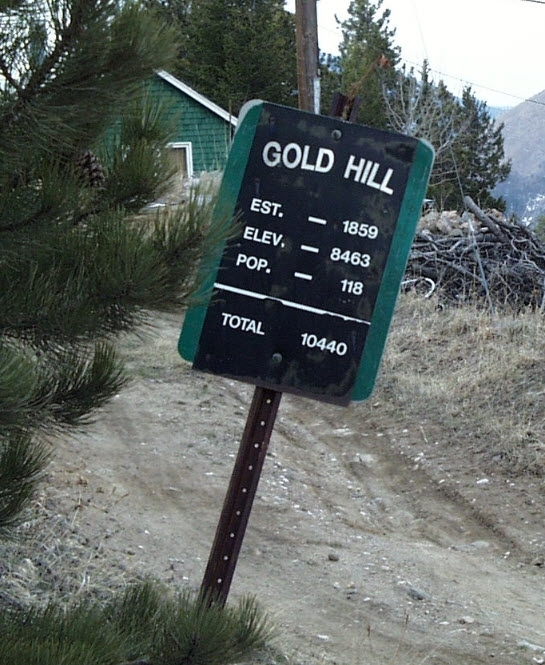
\includegraphics[width=5cm]{type-error}
\par\end{centering}
\caption{A nonsensical calculation arises when mixing incompatible data types.}
\label{nonsense-math}
\end{figure}

The power of the basic principles of mathematics extends over all
epochs and all cultures; they are the same in Rio de Janeiro, in Kuala-Lumpur,
and even in Pyongyang (see Fig.\ \ref{code-without-bugs}).

\section{Functional programming is math}

The functional programming paradigm is based on similar principles:
values are immutable, data processing is coded through formula-like
expressions, and each type of data is required to match correctly
during the computations. A flexible system of data types helps programmers
automatically prevent many kind of coding errors. In addition, modern
programming languages such as Scala and Haskell have a set of features
adapted to building powerful abstractions and domain-specific languages.
This power of abstraction is not accidental. Since mathematics is
the ultimate art of building abstractions, math-based functional programming
languages capitalize on the advantage of several millennia of mathematical
experience.

A prominent example of how mathematics informs the design of programming
languages is the connection between \href{https://en.wikipedia.org/wiki/Intuitionistic_logic}{constructive logic}
and the programming language's type system, called the \href{https://en.wikipedia.org/wiki/Curry\%E2\%80\%93Howard_correspondence}{Curry-Howard (CH) correspondence}.
The main idea of the CH correspondence\index{Curry-Howard correspondence}
is to think of programs as mathematical formulas that compute a value
of a certain type $A$. The CH correspondence is between programs
and logical propositions. To any program that computes a value of
type $A$, there corresponds a proposition stating that ``a value
of type $A$ can be computed''.

This may sound rather theoretical so far. To see the real value of
the CH correspondence, recall that formal logic has operations ``\textbf{\emph{and}}'',
``\textbf{\emph{or}}'', and ``\textbf{\emph{implies}}''. For any
two propositions $A$, $B$, we can construct the propositions ``$A$
\textbf{\emph{and}} $B$'', ``$A$ \textbf{\emph{or}} $B$'', ``$A$
\textbf{\emph{implies}} $B$''. These three logical operations are
foundational; without one of them, the logic is \emph{incomplete}
(you cannot derive some theorems).

A programming language \textbf{obeys the CH correspondence}\index{Curry-Howard correspondence}
to the logic if for any two types $A$, $B$, the language also contains
composite types corresponding to the logical formulas ``$A$ \textbf{\emph{or}}
$B$'', ``$A$ \textbf{\emph{and}} $B$'', ``$A$ \textbf{\emph{implies}}
$B$''. In Scala, these composite types are \texttt{Either{[}A,B{]}},
the tuple \texttt{(A,B)}, and the function type, \texttt{A$\Rightarrow$B}.
All modern functional languages such as OCaml, Haskell, Scala, F\#,
Swift, Rust, Elm, PureScript support these three type constructions
and thus are faithful to the CH correspondence. Having a \emph{complete}
logic in a language's type system enables \href{https://fsharpforfunandprofit.com/ddd/}{declarative domain-driven code design}.

It is interesting to note that most older programming languages (C/C++,
Java, JavaScript, Python) do not support some of these composite types.
In other words, these programming languages have type systems based
on an incomplete logic. As a result, users of these languages have
to implement burdensome workarounds that make for error-prone code.
Failure to follow mathematical principles has real costs.

\begin{figure}
\begin{centering}

\includegraphics[width=0.75\textwidth]{no-bugs}
\par\end{centering}
\caption{The Pyongyang method of error-free programming.}
\label{code-without-bugs}
\end{figure}


\section{The power of abstraction}

Data engineering at scale poses problems of such complexity that many
software companies adopt functional programming languages as their
main implementation tool. Netflix, LinkedIn, Twitter started using
Scala early on and were able to reap the benefits of the powerful
abstractions Scala affords, such as asynchronous streams and parallelized
functional collections. In this way, Scala enabled these businesses
to engineer and scale up their massively concurrent computations.
What exactly makes Scala suitable for big data processing?

The only way to manage massively concurrent code is to use sufficiently
high-level abstractions that make application code declarative. The
two most important such abstractions are the ``resilient distributed
dataset'' (RDD) of Apache Spark and the ``reactive stream'' used
in systems such as Kafka, Apache Storm, Akka Streams, and Apache Flink.
While these abstractions are certainly implementable in Java or Python,
true declarative and type-safe usage is possible only in a programming
language with a sufficiently sophisticated functional type system.
Among the currently available mature functional languages, only Scala
and Haskell would be technically adequate for that task, due to their
support for type classes and higher-order generic collections.

It remains to see why Scala became the \emph{lingua franca} of big
data and not, say, Haskell.

\section{Scala is Java on math }

The recently invented general-purpose functional programming languages
can be grouped into ``industrial'' (F\#, Scala, Swift) and ``academic''
(OCaml, Haskell).

The ``academic'' languages are clean-room implementations of well-researched
mathematical principles of programming language design (the CH correspondence
being one such principle). These languages are unencumbered by requirements
of compatibility with any existing platform or libraries. Because
of this, the ``academic'' languages are perfect playgrounds for
taking various mathematical ideas to their logical conclusion. At
the same time, software practitioners struggle to adopt these languages
due to a steep learning curve, a lack of enterprise-grade libraries
and tool support, and immature package management.

The languages from the ``industrial'' group are based on existing
and mature software ecosystems: F\# on .NET, Scala on JVM, and Swift
on Apple's Cocoa/iOS platform. One of the important design requirements
for these languages is 100\% binary compatibility with their ``parent''
platforms and languages (F\# with C\#, Scala with Java, and Swift
with Objective-C). Because of this, developers can immediately take
advantage of the existing tooling, package management, and industry-strength
libraries, while slowly ramping up the idiomatic usage of new language
features. However, the same compatibility requirement necessitated
certain limitations in the languages, making their design less than
fully satisfactory from the functional programming viewpoint.

It is now easy to see why the adoption rate of the ``industrial''
group of languages is \href{https://www.tiobe.com/tiobe-index/}{much higher}
than that of the ``academic'' languages. The transition to the functional
paradigm is also made smoother for software developers because F\#,
Scala, and Swift seamlessly support the familiar object-oriented programming
paradigm. At the same time, these new languages still have logically
complete type systems, which gives developers an important benefit
of type-safe domain modeling.

Nevertheless, the type systems of these languages are not equally
powerful. For instance, F\# and Swift are similar to OCaml in many
ways but omit OCaml's parameterized modules and some other features.
Of all mentioned languages, Scala and Haskell are the only ones that
directly support type classes and higher-order generics, which are
necessary for expressing abstractions such as an automatically parallelized
data set or an asynchronous data stream.

To see the impact of these advanced features of Scala and Haskell,
consider LINQ, a domain-specific language for database queries on
.NET, implemented in C\# and F\# through a special syntax supported
by Microsoft's compilers. Analogous functionality is provided in Scala
as a \emph{library}, without need to modify the Scala compiler, by
several open-source projects such as Slick, Squeryl, or Quill. Similar
libraries exist for Haskell\textemdash but are impossible to implement
in languages with less powerful type systems.

\section{Conclusion}

The decisive advantages of Scala over other contenders (such as OCaml,
Haskell, F\#, Swift, or Rust) are
\begin{enumerate}
\item functional collections in the standard library;
\item a highly sophisticated type system, with support for type classes
and higher-order generics; 
\item seamless compatibility with a mature software ecosystem (JVM). 
\end{enumerate}
Based on this assessment, we may be confident in Scala's great future
as a main implementation language for big data engineering. 

\appendix

\chapter{Notations}

\section{Summary table}
\begin{description}
\item [{$F^{A}$}] type constructor $F$ with type argument $A$
\item [{$x^{:A}$}] value $x$ has type $A$
\item [{$A+B$}] the disjunction type; in Scala, \texttt{Either{[}A, B{]}} 
\item [{$A\times B$}] the product type; in Scala, \texttt{(A,B)} 
\item [{$A\Rightarrow B$}] the function type, mapping from $A$ to $B$ 
\item [{$\triangleq$}] ``equal by definition'' 
\item [{$\cong$}] ``equivalent'' according to an established isomorphism
of types
\item [{$\left(A\right)^{:F^{B}}$}] type indices for defining unfunctors
(GADTs) 
\item [{$\text{fmap}_{F}$}] the standard method $\text{fmap}$ pertaining
to the functor $F$ 
\item [{$\text{pure}_{F}$}] the standard method $\text{pure}$ of a monad
$F$ 
\item [{$F^{\bullet}$}] the type constructor $F$ understood as a type-level
function; in Scala, \texttt{F{[}\_{]}} 
\item [{$F^{\bullet}\leadsto G^{\bullet}$}] or $F^{A}\leadsto G^{A}$
a natural transformation between functors $F$ and $G$ 
\item [{$\forall A.P^{A}$}] a universally quantified type expression 
\item [{$\exists A.P^{A}$}] an existentially quantified type expression 
\item [{$\bef$}] the forward composition of functions: $f\bef g$ is $x\Rightarrow g(f(x))$.
\item [{$\circ$}] the backward composition of functions: $f\circ g$ is
$x\Rightarrow f(g(x))$. 
\item [{$\circ$}] functor composition: $F\circ G$ is $F^{G^{\bullet}}$ 
\item [{$f^{\uparrow G}$}] a function $f$ lifted to a functor $G$; same
as $\text{fmap}_{G}f$
\item [{$f^{\uparrow G\uparrow H}$}] a function lifted first to $G$ and
then to $H$; In Scala, \texttt{h.map(\_.map(f))} 
\item [{$f^{\downarrow H}$}] a function $f$ lifted to a contrafunctor 
\item [{$\diamond_{M}$}] the Kleisli product operation for the monad $M$ 
\end{description}

\section{Explanations}

$F^{A}$ means a type constructor $F$ with a type argument $A$.
In Scala, this is \texttt{F{[}A{]}}.

$x^{:A}$ means a value $x$ that has type $A$. The colon, $:$,
in the superscript is to show that it is not a type argument. In Scala,
this is \texttt{x : A}. The notation $x:A$ is used as well, but $x^{:A}$
is easier to read when $x$ is inside a code expression. 

$A+B$ means the disjunction type made of types $A$ and $B$. In
Scala, this is the type expression \texttt{Either{[}A, B{]}}.

$A\times B$ means the product type made of types $A$ and $B$. In
Scala, this is the tuple \texttt{(A,B)}.

$A\Rightarrow B$ means a function type from $A$ to $B$. In Scala,
this is the function type \texttt{A $\Rightarrow$ B}.

$\triangleq$ means ``equal by definition''. Examples:
\begin{itemize}
\item $f\triangleq x^{:\text{Int}}\Rightarrow x+1$ is a definition of the
function $f$. In Scala, this is \texttt{val f = (x: Int) $\Rightarrow$
x + 1}.
\item $F^{A}\triangleq1+A$ is a definition of a type constructor $F$.
In Scala, this is \texttt{type F{[}A{]} = Option{[}A{]}}. 
\end{itemize}
$\cong$ means ``equivalent'' according to an equivalence relation
that needs to be established in the text. For example, if we have
established the equivalence that allows nested tuples to be reordered
whenever needed, we can write $\left(a\times b\right)\times c\cong a\times\left(b\times c\right)$.

$\left(A\right)^{:F^{B}}$ in type expressions means that the type
constructor $F^{\bullet}$ assigns the type $F^{B}$ to the type expression
$A$. This is used in defining unfunctors (GADTs) such as $F^{A}\triangleq1^{:F^{\text{Int}}}+A^{:F^{A\times\text{String}}}$.
In Scala, this is
\begin{lyxcode}
sealed~trait~F{[}A{]}

case~class~F1()~extends~F{[}Int{]}

case~class~F2(a:~A)~extends~F{[}(A,~String){]}
\end{lyxcode}
$\text{fmap}_{F}$ means the standard method $\text{fmap}$ pertaining
to the functor $F$. In Scala, this is typically implemented as \texttt{Functor{[}F{]}.fmap()}.
Since each functor $F$ has its own specific definition of $\text{fmap}$,
the subscript ``$F$'' is not a type parameter of $\text{fmap}_{F}$.
The method $\text{fmap}_{F}$ actually has \emph{two} type parameters,
and its type signature written in full is $\text{fmap}_{F}^{A,B}:\left(A\Rightarrow B\right)\Rightarrow F^{A}\Rightarrow F^{B}$.
For clarity, one may write explicitly the type parameters $A,B$ in
the expression $\text{fmap}_{F}^{A,B}$, but in most cases these type
parameters $A$, $B$ may be omitted. 

Similarly, a monad's standard method $\text{pure}_{F}$ has the subscript
denoting its monad $F$. This function has type signature $A\Rightarrow F^{A}$
that contains a type parameter $A$. If we are using this method with
a complicated type, e.g. $1+P^{A}$, instead of $A$, we might want
to indicate this type for clarity as a type parameter and write $\text{pure}_{F}^{1+P^{A}}$.
The type signature of that function is 
\[
\text{pure}_{F}^{1+P^{A}}:1+P^{A}\Rightarrow F^{1+P^{A}}\quad.
\]

$F^{\bullet}$ means the type constructor $F$ understood as a type-level
function, \textendash{} that is, with a type argument unspecified.
In Scala, this is \texttt{F{[}\_{]}}. The bullet symbol, $\bullet$,
is used as a placeholder for the missing type parameter. I also simply
write $F$ when no type argument is needed, and it means the same
as $F^{\bullet}$. (For example, ``a functor $F$'' and ``a functor
$F^{\bullet}$'' mean the same thing.) However, it is useful for
clarity to be able to indicate the place where the type argument would
appear. For instance, functor composition is clearly denoted as $F^{G^{\bullet}}$;
in Scala, this is \texttt{F{[}G{[}?{]}{]}} when using the ``kind
projector'' plugin. As another example, $T_{L}^{M,\bullet}$ denotes
a monad transformer for the base monad $L$ and the foreign monad
$M$. The foreign monad $M$ is a type parameter in $T_{L}^{M,\bullet}$,
and so is the missing type parameter denoted by the placeholder symbol
$\bullet$. (However, the base monad $L$ is not a type parameter
in $T_{L}^{M,\bullet}$ because the construction of the monad transformer
depends sensitively on the internal details of $L$.)

$F^{\bullet}\leadsto G^{\bullet}$ or $F^{A}\leadsto G^{A}$ means
a natural transformation between two functors $F$ and $G$.

$\forall A.P^{A}$ is a universally quantified type expression, in
which $A$ is a bound type parameter.

$\exists A.P^{A}$ is an existentially quantified type expression,
in which $A$ is a bound type parameter.

$\bef$ means the forward composition\index{forward composition}
of functions: $f\bef g$ (reads ``$f$ before $g$'') is the function
defined as $x\Rightarrow g(f(x))$.

$\circ$ means the backward composition\index{backward composition}
of functions: $f\circ g$ (reads ``$f$ after $g$'') is the function
defined as $x\Rightarrow f(g(x))$. 

$\circ$ with type constructors means their functor composition, for
example $F\circ G$ is the same as the functor $F^{G^{\bullet}}$.
In Scala, this is \texttt{F{[}G{[}A{]}{]}}. 

$f^{\uparrow G}$ means a function $f$ lifted to a functor $G$.
For a function $f^{:A\Rightarrow B}$, the application of $f^{\uparrow G}$
to a value $g:G^{A}$ is written as $f^{\uparrow G}g$. In Scala,
this is \texttt{g.map(f)}. Nested liftings can be written as $f^{\uparrow G\uparrow H}$,
which means $\left(f^{\uparrow G}\right)^{\uparrow H}$ and produces
a function of type $H^{G^{A}}\Rightarrow H^{G^{B}}$ . Applying a
nested lifting to a value $h$ of type $H^{G^{A}}$ is written as
$f^{\uparrow G\uparrow H}h$. In Scala, this is \texttt{h.map(\_.map(f))}. 

$f^{\downarrow H}$ means a function $f$ lifted to a contrafunctor
$H$. For a function $f^{:A\Rightarrow B}$, the application of $f^{\downarrow H}$
to a value $h:H^{B}$ is written as $f^{\uparrow H}h$ and yields
a value of type $H^{A}$. In Scala, this is \texttt{h.contramap(f)}.

$\diamond_{M}$ means the Kleisli product operation for the monad
$M$. This is a binary operation working on two Kleisli functions
of types $A\Rightarrow M^{B}$ and $B\Rightarrow M^{C}$ and yields
a new function of type $A\Rightarrow M^{C}$. 

\chapter{Glossary of terms}

I chose certain terms in this book to be different from the terms
currently used in the functional programming community. My proposed
terminology is designed to help readers understand and remember the
concepts behind the terms. 
\begin{description}
\item [{\index{Nameless�function}Nameless~function}] An expression of
function type, representing a function. For example, \texttt{x $\Rightarrow$
x {*} 2}. Also known as function expression, function literal, anonymous
function, closure, lambda-function, lambda-expression, or simply a
``lambda''.
\item [{\index{Product�type}Product~type}] A type representing several
values given at once. In Scala, product types are the tuple types,
for example \texttt{(Int, String)}, and case classes. Also known as
\textbf{tuple} type, \textbf{struct} (in C and C++), and \textbf{record}.
\item [{\index{Disjunction�type}Disjunction~type}] A type representing
one of several distinct possibilities. In Scala, this is usually implemented
as a sealed trait extended by several case classes. The standard Scala
disjunction types are \texttt{Option{[}A{]}} and \texttt{Either{[}A,
B{]}}. Also known as \textbf{sum }type, \textbf{co-product\index{co-product}}
type, and variant type (in OCaml and in Object Pascal). It is shorter
to say ``sum type,'' but the English word ``sum'' is more ambiguous
to the ear than ``disjunction''.
\item [{\index{Polynomial�functor}Polynomial~functor}] A type constructor
built using disjunctions (sums), products (tuples), type parameters
and fixed types. For example, in Scala, \texttt{type F{[}A{]} = Either{[}(Int,
A), A{]}} is a polynomial functor with respect to the type parameter
$A$, while \texttt{Int} is a fixed type (not a type parameter). Polynomial
functors are also called \textbf{algebraic data types}\index{algebraic data type}.
A polynomial type constructor is always a functor with respect to
any of its type parameters, hence I use the shorter name ``polynomial
functor'' instead of ``polynomial type constructor''.
\item [{Unfunctor\index{unfunctor}}] A type constructor that cannot possibly
be a functor, nor a contrafunctor, nor a profunctor. An example is
a type constructor with explicitly indexed type parameters, such as
$F^{A}\triangleq\left(A\times A\right)^{:F^{\text{Int}}}+\left(\text{Int}\times A\right)^{:F^{1}}$.
Also called a \textbf{\index{GADT (generalized algebraic data type)}GADT}
(generalized algebraic data type).
\item [{Functor~block}] \index{functor block} A short syntax for composing
various \texttt{map}, \texttt{flatMap}, and \texttt{filter} operations
on a functor value. The \texttt{Functor} typeclass instance must be
fixed for the entire functor block. For example, in Scala the code
\\
\texttt{for \{ x $\leftarrow$ List(1,2,3); y $\leftarrow$ List(10,
x); if y > 2 \}}~\\
\texttt{~ ~ yield 2 {*} y} \\
is equivalent to the code \\
\texttt{List(1,2,3).flatMap(x $\rightarrow$ List(10, x))}~\\
\texttt{~ ~ .filter(y $\Rightarrow$ y > 1).map(y $\Rightarrow$
2 {*} y)}\\
 and computes the value \texttt{List(20, 20, 20, 6)}. Similar syntax
exists in a number of languages and is called a \textbf{for-comprehension\index{for-comprehension}}
or \textbf{list comprehension} (in Python), \textbf{do-notation\index{do-notation (Haskell)}}
or do-block (in Haskell), and \textbf{computation expressions\index{computation expressions (F##)@computation expressions (F\#\#)}}
(in F\#). I use the name ``functor block'' in this book because
it is shorter and more descriptive.
\item [{Method\index{method}}] 1) A function defined as a member of a
typeclass. For example, \texttt{flatMap} is a method defined in the
\texttt{Monad} typeclass. 2) In Scala, a function defined as a member
of a data type declared as a Java-compatible \texttt{class} or \texttt{trait}.
Trait methods are necessary in Scala when implementing functions whose
arguments have type parameters (because ordinary Scala function values
cannot have type parameters). So, many type classes such as \texttt{Functor}
or \texttt{Monad}, whose methods$_{1}$ require type parameters, will
use Scala \texttt{trait}s with methods\emph{$_{2}$} for their implementation.
The same applies to type constructions with quantified types, such
as Church encoding. 
\item [{\index{Kleisli�function}Kleisli~function}] Also called a Kleisli
morphism\index{Kleisli morphism} or a \index{Kleisli arrow}Kleisli
arrow. A function with type signature $A\Rightarrow M^{B}$ for some
fixed monad $M$. More verbosely, ``a morphism from the Kleisli category
corresponding to the monad $M$''. The standard monadic method $\text{pure}_{M}:A\Rightarrow M^{A}$
has the type signature of a Kleisli function. The Kleisli product
operation, $\diamond_{M}$, is a binary operation that combines two
Kleisli functions (of types $A\Rightarrow M^{B}$ and $B\Rightarrow M^{C}$)
into a new Kleisli function (of type $A\Rightarrow M^{C}$).
\item [{\index{exponential-polynomial�type}Exponential-polynomial~type}] A
type constructor built using disjunctions (sums), products, and function
types, as well as type parameters or fixed types. For brevity, I call
them ``exp-poly'' types. For example, in Scala, \texttt{type F{[}A{]}
= Either{[}(A, A), Int $\Rightarrow$ A{]}} is an exp-poly type constructor.
Such type constructors can be functors, contrafunctors, or profunctors.
\item [{\index{Short�type�notation}Short~type~notation}] A mathematical
notation for type expressions developed in this book for the purpose
of quicker and more practical reasoning about types in functional
programs. Disjunction types are denoted by $+$, product types by
$\times$, and function types by $\Rightarrow$. The unit type is
denoted by $1$, and the void type by $0$. The function arrow $\Rightarrow$
has weaker precedence than $+$, which is in turn weaker than $\times$.
Type parameters are denoted by superscripts. As an example of using
these conventions, the Scala definition
\begin{lyxcode}
type~F{[}A{]}~=~Either{[}(A,~A~$\Rightarrow$~Option{[}Int{]}),~String~$\Rightarrow$~List{[}A{]}{]}
\end{lyxcode}
is written in the short type notation as 
\[
F^{A}\triangleq A\times\left(A\Rightarrow1+\text{Int}\right)+\left(\text{String}\Rightarrow\text{List}^{A}\right)\quad.
\]

\end{description}

\section{On the current misuse of the term ``algebra''}

In this book, I do not use the terms ``algebra\index{algebra}''
or ``algebraic\index{algebraic}'', because these terms are too
ambiguous. In the current practice, the functional programming community
is using the word ``algebra'' in at least \emph{four} incompatible
ways.

\paragraph{Definition 0.}

In mathematics, an \textquotedblleft algebra\textquotedblright{} is
a vector space with multiplication and certain standard properties.
For example, you need $1*x=x$, the addition must be commutative,
the multiplication must be distributive over addition, and so on.
As an example, the set of all $10\times10$ matrices with real coefficients
is an \textquotedblleft algebra\textquotedblright{} in this sense.
These matrices form a $100$-dimensional vector space, and can be
multiplied and added. This standard definition of ``algebra'' is
not actually used in functional programming.

\paragraph{Definition 1.}

An ``algebra'' is a function with type signature $F^{A}\Rightarrow A$,
where $F^{A}$ is some fixed functor. This definition comes from category
theory, where such types are called \textbf{$F$-algebras\index{$F$-algebra}}.
There is no direct connection between this ``algebra'' and Definition~0,
except when the functor $F$ is defined by $F^{A}\triangleq A\times A$,
and then a function of type $A\times A\Rightarrow A$ may be interpreted
as a ``multiplication'' operation (but, in any case, $A$ is a type
and not a vector space, and there are no distributivity or commutativity
laws). I prefer to call such functions ``$F$-algebras'', emphasizing
that they characterize and depend on a chosen functor $F$. However,
$F$-algebras are not mentioned in this book: knowing how to reason
about their properties does not give much help in practical work.

\paragraph{Definition 2.}

Polynomial functors are often called \textquotedblleft algebraic data
types\textquotedblright . However, they are not \textquotedblleft algebraic\textquotedblright{}
in the sense of Definition~0 or 1. For example, consider the \textquotedblleft algebraic
data type\textquotedblright{} \texttt{Either{[}Option{[}A{]}, Int{]},}
or $F^{A}\triangleq1+A+\text{Int}$ in the short type notation. The
set of all values of the type $F^{A}$ does not admit the addition
and multiplication operations required by the mathematical definition
of ``algebra''. The type $F^{A}$ may admit some binary or unary
operations (e.g.~that of a monoid), but these operations will not
be commutative or distributive. Also, there cannot be a function with
type $F^{A}\Rightarrow A$, as required for Definition~1. It seems
that the usage of the word ``algebra'' here is to refer to ``school-level
algebra'' with polynomials; these data types are built from sums
and products of types. In this book, I call such types ``polynomial''.
However, if the data type contains a function type, e.g.~\texttt{Option{[}Int
$\Rightarrow$ A{]}}, the type is no longer polynomial. So I use the
more precise terms \textquotedblleft polynomial type\textquotedblright{}
and \textquotedblleft exponential-polynomial type\textquotedblright .

\paragraph{Definition 3.}

People talk about the \textquotedblleft algebra\textquotedblright{}
of properties of functions such as \texttt{map} or \texttt{flatMap},
referring to the fact that these functions must satisfy certain equational
laws (e.g.~the identity, composition, or associativity laws). But
these laws do not form an ``algebra'' in the sense of Definition
0, nor do the functions such as \texttt{map} or \texttt{flatMap} themselves
(there are no binary operations on them). Neither do they form an
algebra in the sense of Definition~1. The laws for \texttt{map} or
\texttt{flatMap} are in no way related to \textquotedblleft algebraic
data types\textquotedblright{} of Definition 2. So here the word \textquotedblleft algebra\textquotedblright{}
is used in a way that is unrelated to the three previous definitions.
To me, it does not seem helpful to say the word ``algebra'' or ``algebraic''
when talking about equational laws. These laws are ``algebraic''
in a trivial sense \textendash{} i.e.~they are written as equations.
In mathematics, ``algebraic'' equations are different from ``differential''
or ``integral'' equations. In functional programming, all equational
laws are of the same kind: some code on the left-hand side must be
equal to some code on the right-hand side of the equation. So calling
them ``algebraic'' does not help and does not clarify anything.
I call them ``equational laws'' or just ``laws''.

\paragraph{Definition 4.}

In the Church encoding of a free monad (nowadays known as the ``final
tagless'' encoding), the term ``algebra'' refers to the \emph{type
constructor} parameter $F$. This definition has nothing to do with
any of the previous definitions. Clearly, Definition~0 cannot apply
to a type constructor. Definition 1 does not apply since $F$ is not
itself a function type of the form $G^{A}\Rightarrow A$. (A function
of type $F^{A}\Rightarrow A$, which I call a ``runner'' for the
type constructor $F$, is not usually called an ``algebra'' in discussions
of the ``final tagless'' encoding.) Definition 2 seems to be the
most closely related meaning, since $F$ is \emph{sometimes} a polynomial
type in practical usage (although in most cases $F$ will be an unfunctor).
However, it is not helpful to call the polynomial functor $F$ an
``algebraic data type'' and, at the same time, an ``algebra''.
Definition 3 does not apply since the free monad construction does
not assume that any laws hold about $F$, nor has any means of imposing
such laws. The type constructor $F$ is used to parameterize the effects
described by the free monad, so it seems more reasonable to call it
the ``effect constructor''.

So, it seems that the current usage of the word ``algebra'' in functional
programming is both inconsistent and unhelpful to practitioners. In
this book, I reserve the word ``algebra'' to denote the branch of
mathematics, as in ``school-level algebra'' or ``graduate-level
algebra''. Instead of ``algebra'' as in Definitions~1 to 4, I
talk about ``$F$-algebras'' with a specific functor $F$; ``polynomial
types'' or ``polynomial functors'' or ``exponential-polynomial
functors'' etc.; ``equational laws''; and an ``effect constructor''
$F$.

\chapter{Scala syntax and features}

\subsection{Function syntax}

Functions have arguments, body, and type. The function type lists
the type of all arguments and the type of the result value.
\begin{lyxcode}
def~f(x:~Int,~y:~Int):~Int~$\Rightarrow$~Int~=~\{~z~$\Rightarrow$~x~+~y~+~z~\}
\end{lyxcode}
Functions may be used with \index{infix syntax}infix syntax as well.
For this syntax to work, the function must be defined \textbf{as a
Scala method}\index{method}\index{Scala method}, that is, using
\texttt{def} within the declaration of \texttt{x}'s class, or as an
extension method. The infix syntax cannot work with functions defined
using \texttt{val}. For clarity, I call Scala functions \textbf{infix
methods}\index{infix method} when defined and used in this way.

The type syntax \texttt{List{[}Int{]}} means ``a list of integer
values.'' In the type expression \texttt{List{[}Int{]}}, the ``\texttt{Int}''
is called the \textbf{type parameter\index{type parameter}} and \texttt{List}
is called the \textbf{type constructor}\index{type constructor}.
A list can contain values of any type; for example, \texttt{List{[}List{[}List{[}Int{]}{]}{]}}
means a list of lists of lists of integers. So, the type constructor
can be seen as a function from types to types: A type constructor
takes a type parameter as an argument, and produces a new type as
a result.

\subsection{Scala collections}

The Scala standard library defines collections of several kinds, the
main ones being sequences, sets, and dictionaries. These collections
have many map/reduce-style methods defined on them.

Sequences are ``subclasses'' of the class \texttt{Seq}. The standard
library will sometimes choose automatically a suitable subclass of
\texttt{Seq}, such as \texttt{List}, \texttt{IndexedSeq}, \texttt{Vector},
\texttt{Range}, etc.; for example:
\begin{lyxcode}
scala>~1~to~5

scala>~(1~to~5).map(x~$\Rightarrow$~x{*}x)

scala>~(1~to~5).toList

scala>~1~until~5

scala>~(1~until~5).toList
\end{lyxcode}
For our purposes, all these ``sequence-like'' types are equivalent.

Sets are values of class \texttt{Set}, and dictionaries are values
of class \texttt{Map}.
\begin{lyxcode}
scala>~Set(1,~2,~3).filter(x~$\Rightarrow$~x~\%~2~==~0)
\end{lyxcode}

\chapter{Intuitionistic (constructive) propositional logic}

The intuitionistic propositional logic describes how programs in functional
programming languages may be able to compute values of different types.

The main difference between IPL and the classical (Boolean) logic
is that IPL does not include the axiom of excluded middle (``\emph{tertium
non datur}''), which is 
\[
\forall A:(A\text{ or }\left(\text{not}A\right))\text{ is true}\quad.
\]
 The reason this axiom is not included in IPL is that IPL propositions
such as ${\cal CH}\left(A\right)$ correspond to the \emph{possibility}
of values of type $A$ \emph{to be computed} by a program. For the
proposition ${\cal CH}\left(A\right)$ to be true in IPL, a program
needs to actually compute a value of type $A$. It is not sufficient
merely to show that the non-existence of such a value would be somehow
contradictory. (In classical logic, that would be sufficient.)

Another significant difference between IPL and the Boolean logic is
that propositions in IPL cannot be assigned a fixed set of ``truth
values''. This was proved by G�del in 1935. It means that a proposition
in IPL cannot be decided by writing out a truth table, even if we
allow many truth values.

\chapter{Category theory}

Examples of categories
\begin{enumerate}
\item Objects: types $\text{Int}$, $\text{String}$, ...; morphisms (arrows)
are functions $\text{Int}\rightarrow\text{String}$ etc. \textendash{}
this is the ``standard'' category corresponding to a given programming
language
\item Objects: types $A$, $B$, ...; morphisms are pairs of functions $\left(A\rightarrow B\right),\left(B\rightarrow A\right)$
\item {*} Objects: types $\text{List}^{A}$, $\text{List}^{B}$, ...; morphisms
are functions of type $\text{List}^{A}\rightarrow\text{List}^{B}$
\item Objects: types $A$, $B$, ...; morphisms are functions of type $\text{List}^{A}\rightarrow\text{List}^{B}$
\item Objects: types $A$, $B$, ...; morphisms are functions of type $A\rightarrow\text{List}^{B}$
\item {*} Objects: types $\text{List}^{A}$, $\text{List}^{B}$, ...; morphisms
are functions $A\rightarrow B$
\item Objects: types $A$, $B$, ...; morphisms are $\text{List}^{A\rightarrow B}$
\item Objects: types $A,$ $B$, ...; morphisms are functions $B\rightarrow A$
\item {*} Objects: things $A,$ $B$, ...; morphisms are pairs $\left(A,B\right)$
of things \textendash{} this is the same as a preorder
\end{enumerate}
Examples marked with {*} are for illustration only, they are probably
not very useful

\chapter{What is ``applied functional type theory''}

\section{The import and scope of AFTT}

\textbf{\index{Applied functional type theory}Applied functional
type theory} (AFTT) is what I call the area of computer science that
should serve the needs of functional programmers who are working as
software engineers.

It is for these practitioners (I am one myself), rather than for academic
researchers, that I set out to examine the incredible wealth of functional
programming inventions over the last 30 years, \textendash{} such
as the \href{https://wiki.haskell.org/Research_papers/Functional_pearls}{\textquotedblleft functional pearls\textquotedblright{} papers}
\textendash{} and to determine the scope of theoretical material that
has demonstrated its pragmatic usefulness and thus belongs to AFTT,
as opposed to material that is purely academic and may be tentatively
omitted.

What exactly is the extent of ``theory'' that a practicing functional
programmer should know in order to be effective at writing code? In
my view, this question is not yet resolved. Once it is resolved, AFTT
will be that theory.

Traditional courses of theoretical computer science (algorithms, traditional
data structures, complexity theory, formal languages, formal semantics,
compiler techniques, databases, networking, operating systems, etc.)
are largely not relevant to AFTT.

Here is an example: To an academic computer scientist, the ``science
behind Haskell'' is the theory of lambda-calculus, the type-theoretic
``System $F\omega$'', and formal semantics. These theories guided
the design of the Haskell language and define rigorously what a Haskell
program ``means'' in a mathematical sense. Academic computer science
courses teach these theories.

However, a practicing Haskell or Scala programmer is not concerned
with designing Haskell or Scala, or with proving any theoretical properties
of those languages. A practicing programmer is mainly concerned with
\emph{using} a chosen programming language to \emph{write code}.

Neither the theory of lambda-calculus, nor proofs of type-theoretical
properties of ``System $F\omega$'', nor theories of formal semantics
will actually help a programmer to write code. So all these theories
are not within the scope of AFTT.

As an example of theoretical material that \emph{is} within the scope
of AFTT, consider the equational laws imposed on applicative functors
(see Chapter~\ref{chap:8-Applicative-functors,-contrafunc}).

It is essential for a practicing functional programmer to be able
to recognize and use applicative functors. An applicative functor
is a data structure can specify declaratively a set of operations
that do not depend on each other's effects. Programs can then easily
combine these operations and effects, for example, in order to execute
them in parallel, or to refactor the program for better maintainability.

To use this functionality, the programmer must begin by checking whether
a given data structure that satisfies the laws of applicative functors.
In a given application, a data structure may be dictated in part by
the business logic that cannot be changed. The programmer first writes
down the type of that data structure and the code implementing the
required methods, and then checks that the laws hold. The data structure
may need to be adjusted in order to fit the definition of an applicative
functor or its laws.

This work is done using pen and paper, in a mathematical notation.
Once the applicative laws are verified, the programmer proceeds to
write code using that data structure.

Because of the proofs, it is assured that the data structure satisfies
the known properties of applicative functors, no matter how the rest
of the program is written. So, for example, it is assured that the
relevant effects can be automatically parallelized, as is usual with
applicative functors.

In this way, AFTT directly guides the programmer and helps to write
correct code.

Applicative functors were discovered by practitioners who were using
Haskell for writing code, in applications such as parser combinators,
compilers, and domain-specific languages for parallel computations.
However, applicative functors are not a feature of Haskell: they are
the same in Scala, OCaml, or any other functional programming language.
And yet, no standard computer science textbook defines applicative
functors, motivates their laws, explores their structure on basic
examples, or shows data structures that are \emph{not} applicative
functors and explains why. (For that matter, no book on category theory
or type theory mentions applicative functors either.)

So far it appears that AFTT will be a mixture of certain areas of
category theory, formal logic, and type theory. However, software
engineers would not derive much benefit from following traditional
academic courses in these subjects, because their choice of material
is too abstract and lacks specific results necessary for practical
software engineering. In other words, the traditional academic courses
answer questions that academic computer scientists have, not questions
that software engineers have.

There exist several books intended as presentations of category theory
``for computer scientists'' or ``for programmers''. However, these
books fail to give examples vitally relevant to everyday programming,
such as applicative or traversable functors. Instead, these books
contain purely theoretical topics such as limits, adjunctions, or
toposes, \textendash{} concepts that have no applications in practical
functional programming today.

Typical questions in academic books: ``is this an introduction or
an elimination rule'' and ``does this property hold in non-small
categories, or are we limited to the category $\mathbb{S}et$''.
Typical questions a Scala programmer might have: ``can we compute
a value of type \texttt{Either{[}Z, R $\Rightarrow$ A{]}} from a
value of type \texttt{R $\Rightarrow$ Either{[}Z, A{]}}'' and ``is
the type constructor \texttt{F{[}A{]} = Option{[}(A, A, A){]}} a monad''.
The proper scope of AFTT includes answering the last two questions,
but not the first two.

A software engineer hoping to understand the foundations of functional
programming will not find the concepts of foldable, filterable, applicative,
or traversable functors in any books on category theory, including
books intended for programmers. And yet, these concepts are necessary
to obtain a mathematically correct implementation of such foundationally
important operations as fold, filter, zip, and traverse \textendash{}
operations that functional programmers use every day in their code.

To compensate for the lack of AFTT textbooks, programmers have written
many online tutorials for each other, trying to explain the theoretical
concepts necessary for practical work. There are the infamous ``monad
tutorials'', but also tutorials about applicative functors, traversable
functors, free monads, and so on. These tutorials tend to be very
hands-on and narrow in scope, limited to one or two specific questions
and specific applications. Such tutorials usually do not present a
sufficiently broad picture and do not illustrate deeper connections
between these mathematical constructions.

For example, ``free monads'' became popular in the Scala community
around 2015. Many talks about free monads were presented at Scala
engineering conferences, each giving their own slightly different
implementation but never formulating rigorously the required properties
for a piece of code to be a valid implementation of the free monad.

Without knowledge of mathematical principles behind free monads, a
programmer cannot make sure that a given implementation is correct.
However, books on category theory present free monads in a way that
is unsuitable for programming applications: a free monad is just an
adjoint functor to a forgetful functor into the category of sets.\footnote{``What's your problem?'' as the joke goes.}
This definition is too abstract and cannot be used to verify whether
a given implementation of the free monad in Scala is correct.

Perhaps the best selection of AFTT tutorial material can be found
in the \href{https://en.wikibooks.org/wiki/Haskell}{Haskell Wikibooks}.
However, those tutorials are incomplete and limited to explaining
the use of Haskell. Many of them are suitable neither as a first introduction
nor as a reference on AFTT.

Apart from referring to some notions from category theory, AFTT also
uses some concepts from type theory and formal logic. However, existing
textbooks on type theory and formal logic focus on domain theory and
proof theory \textendash{} which is a lot of information that practicing
programmers will have difficulty assimilating and yet will have no
chance of ever applying in their daily work. At the same time, these
books never mention practical techniques used in many functional programming
libraries today, such as quantified types, types parameterized by
type constructors, or partial type-level functions (known as ``typeclasses'').

Type theory and formal logic can, in principle, help the programmer
with certain practical tasks, such as:
\begin{itemize}
\item deciding whether two data structures are equivalent as types, and
implementing the isomorphism transformation; for example, the Scala
type \texttt{(A, Either{[}B, C{]})} is equivalent to \texttt{Either{[}(A,
B), (A, C){]}} 
\item detecting whether a definition of a recursive type is ``valid'',
i.e.~does not lead to a useless infinite recursion; an example of
a ``useless'' recursive type definition in Scala is \texttt{case
class Bad(x: Bad)} 
\item deriving an implementation of a function from its type signature and
required laws; for example, deriving the \texttt{flatMap} function
for the \texttt{Reader} monad from the type signature \texttt{def
flatMap{[}Z, A, B{]}(r: Z \ensuremath{\Rightarrow} A)(f: A \ensuremath{\Rightarrow}
Z \ensuremath{\Rightarrow} B): Z \ensuremath{\Rightarrow} B} and verifying
that the monad laws hold
\item deciding whether a generic pure function with a given signature can
be implemented; for example, \texttt{def f{[}A, B{]}: (A \ensuremath{\Rightarrow}
B) \ensuremath{\Rightarrow} A} cannot be implemented but \texttt{def
g{[}A, B{]}: A \ensuremath{\Rightarrow} (B \ensuremath{\Rightarrow}
A)} can be implemented 
\end{itemize}
I mention these practical tasks as examples because they are perhaps
the only real-world-coding applications of domain theory and the Curry-Howard
correspondence theory, besides programming language design. However,
existing books on type theory and logic do not give practical recipes
for resolving these questions.

On the other hand, books such as \href{https://underscore.io/books/scala-with-cats/}{\textquotedblleft Scala with Cats\textquotedblright}
and \href{https://alvinalexander.com/scala/functional-programming-simplified-book}{\textquotedblleft Functional programming, simplified\textquotedblright}
are focused on explaining the practical aspects of programming and
do not adequately treat the algebraic laws that the mathematical structures
require (such as the laws for applicative or monadic functors).

The only existing Scala-based AFTT textbook aiming at the proper scope
is the \href{https://www.manning.com/books/functional-programming-in-scala}{Bjarnason-Chiusano book},
which balances practical considerations with theoretical developments
such as algebraic laws. This book is written at about the same level
but goes deeper into the mathematical foundations and at the same
time gives a wider range of examples.

This book is an attempt to delineate the proper scope of AFTT and
to develop a rigorous yet clear and approachable presentation of the
chosen material. The goal is to teach programmers how to reason mathematically
about types and code, in a way that is directly relevant to practical
programming.

In this book, I demonstrate code examples in Scala because this is
what I am most familiar with. However, most of this material will
work equally well in Haskell, OCaml, and other FP languages. This
is so because AFTT is not specific to Scala or Haskell. A serious
user of any other functional programming language will have to face
the same questions and struggle with the same practical issues.

\section{Approach to presentation}

The presentation is self-contained. I introduce and explain all the
required notations, concepts, and Scala language features. The emphasis
is on clarity and understandability of all examples, mathematical
notions, derivations, and code. I introduce a fair amount of non-standard
terminology and notations because this allows me to to achieve a clearer
and more logically coherent presentation of the material, especially
for readers not familiar with the theoretical literature.

The main content of AFTT is to expose mathematical principles that
guide the practice of functional programming \textendash{} that is,
help people to write code. Therefore, all mathematical developments
in this book are thoroughly motivated by practical programming issues.

Each mathematical construction is accompanied by code examples and
unit tests to illustrate its usage and check correctness. For example,
the equational laws for every standard typeclass (functor, applicative,
monad, etc.) are first motivated heuristically before deriving a set
of mathematical equations and formulating the laws in terms of axioms
of a category. In this book, all theory is developed in order to write
some new code as a result, and in order to answer a question arising
from programming practice. Theoretical material from category theory,
type theory, and formal logic is kept to the absolute minimum necessary.
Mathematical generalizations are not pursued beyond either practical
usefulness or immediate pedagogical usefulness. This limits the scope
of required mathematical knowledge to bare rudiments of category theory,
type theory, and formal logic. For instance, I never mention ``introduction/elimination
rules'', ``strong normalization'', ``complete partial order domain'',
``adjoint functor'', ``pullback'', ``pushout'', ``limit'',
``co-limit'', or the word ``algebra'', because using these concepts
will not help a functional programmer to write code. Instead, I focus
on practically useful material \textendash{} including some little-known
but useful constructions such as the ``partial type function'',
``filterable'' and ``applicative contrafunctor'' typeclasses,
and ``free pointed'' monad. 

Each new concept or technique is fully explained via ``worked examples''
and drilled via provided exercises. Answers to exercises are not provided,
but it is verified that the exercises are doable and free of errors.
More difficult exercises are marked by an asterisk.

\section{Intended audience }

The material is presented here at medium to advanced level. It requires
a certain amount of mathematical experience and is not suitable for
people unfamiliar with school-level algebra, or for people who are
generally allergic to mathematics, or for people unwilling to learn
new and difficult concepts through prolonged mental concentration.

The first two chapters are introductory and may be suitable for beginners
in programming. Starting from the middle of chapter 3, the material
becomes unsuitable for beginners.

\chapter{GNU Free Documentation License\label{sec:GFDL} }

{\tiny{}Version 1.2, November 2002}{\tiny\par}

{\tiny{}Copyright (c) 2000,2001,2002 Free Software Foundation, Inc.
59 Temple Place, Suite 330, Boston, MA 02111-1307, USA}{\tiny\par}

{\tiny{}Everyone is permitted to copy and distribute verbatim copies
of this license document, but changing it is not allowed.}{\tiny\par}

{\tiny{}\setcounter{subsection}{-1}}{\tiny\par}

\subsection*{{\tiny{}Preamble}}

{\tiny{}The purpose of this License is to make a manual, textbook,
or other functional and useful document free in the sense of freedom:
to assure everyone the effective freedom to copy and redistribute
it, with or without modifying it, either commercially or noncommercially.
Secondarily, this License preserves for the author and publisher a
way to get credit for their work, while not being considered responsible
for modifications made by others.}{\tiny\par}

{\tiny{}This License is a kind of \textquotedblleft copyleft'', which
means that derivative works of the document must themselves be free
in the same sense. It complements the GNU General Public License,
which is a copyleft license designed for free software.}{\tiny\par}

{\tiny{}We have designed this License in order to use it for manuals
for free software, because free software needs free documentation:
a free program should come with manuals providing the same freedoms
that the software does. But this License is not limited to software
manuals; it can be used for any textual work, regardless of subject
matter or whether it is published as a printed book. We recommend
this License principally for works whose purpose is instruction or
reference.}{\tiny\par}

\subsection{Applicability and definitions\label{subsec:1Applicability-and-definitions}}

{\tiny{}This License applies to any manual or other work, in any medium,
that contains a notice placed by the copyright holder saying it can
be distributed under the terms of this License. Such a notice grants
a world-wide, royalty-free license, unlimited in duration, to use
that work under the conditions stated herein. The \textquotedblleft Document'',
below, refers to any such manual or work. Any member of the public
is a licensee, and is addressed as \textquotedblleft you''. You accept
the license if you copy, modify or distribute the work in a way requiring
permission under copyright law.}{\tiny\par}

{\tiny{}A \textquotedblleft Modified Version'' of the Document means
any work containing the Document or a portion of it, either copied
verbatim, or with modifications and/or translated into another language.}{\tiny\par}

{\tiny{}A \textquotedblleft Secondary Section'' is a named appendix
or a front-matter section of the Document that deals exclusively with
the relationship of the publishers or authors of the Document to the
Document's overall subject (or to related matters) and contains nothing
that could fall directly within that overall subject. (Thus, if the
Document is in part a textbook of mathematics, a Secondary Section
may not explain any mathematics.) The relationship could be a matter
of historical connection with the subject or with related matters,
or of legal, commercial, philosophical, ethical or political position
regarding them.}{\tiny\par}

{\tiny{}The \textquotedblleft Invariant Sections'' are certain Secondary
Sections whose titles are designated, as being those of Invariant
Sections, in the notice that says that the Document is released under
this License. If a section does not fit the above definition of Secondary
then it is not allowed to be designated as Invariant. The Document
may contain zero Invariant Sections. If the Document does not identify
any Invariant Sections then there are none.}{\tiny\par}

{\tiny{}The \textquotedblleft Cover Texts'' are certain short passages
of text that are listed, as Front-Cover Texts or Back-Cover Texts,
in the notice that says that the Document is released under this License.
A Front-Cover Text may be at most 5 words, and a Back-Cover Text may
be at most 25 words.}{\tiny\par}

{\tiny{}A \textquotedblleft Transparent'' copy of the Document means
a machine-readable copy, represented in a format whose specification
is available to the general public, that is suitable for revising
the document straightforwardly with generic text editors or (for images
composed of pixels) generic paint programs or (for drawings) some
widely available drawing editor, and that is suitable for input to
text formatters or for automatic translation to a variety of formats
suitable for input to text formatters. A copy made in an otherwise
Transparent file format whose markup, or absence of markup, has been
arranged to thwart or discourage subsequent modification by readers
is not Transparent. An image format is not Transparent if used for
any substantial amount of text. A copy that is not \textquotedblleft Transparent''
is called \textquotedblleft Opaque''.}{\tiny\par}

{\tiny{}Examples of suitable formats for Transparent copies include
plain ASCII without markup, Texinfo input format, \LaTeX{} input format,
SGML or XML using a publicly available DTD, and standard-conforming
simple HTML, PostScript or PDF designed for human modification. Examples
of transparent image formats include PNG, XCF and JPG. Opaque formats
include proprietary formats that can be read and edited only by proprietary
word processors, SGML or XML for which the DTD and/or processing tools
are not generally available, and the machine-generated HTML, PostScript
or PDF produced by some word processors for output purposes only.}{\tiny\par}

{\tiny{}The ``Title Page'' means, for a printed book, the title
page itself, plus such following pages as are needed to hold, legibly,
the material this License requires to appear in the title page. For
works in formats which do not have any title page as such, \textquotedblleft Title
Page\textquotedblright{} means the text near the most prominent appearance
of the work's title, preceding the beginning of the body of the text.}{\tiny\par}

{\tiny{}A section ``Entitled XYZ'' means a named subunit of the
Document whose title either is precisely XYZ or contains XYZ in parentheses
following text that translates XYZ in another language. (Here XYZ
stands for a specific section name mentioned below, such as \textquotedblleft Acknowledgements\textquotedblright ,
\textquotedblleft Dedications\textquotedblright , \textquotedblleft Endorsements\textquotedblright ,
or \textquotedblleft History\textquotedblright .) To \textquotedblleft Preserve
the Title\textquotedblright{} of such a section when you modify the
Document means that it remains a section \textquotedblleft Entitled
XYZ\textquotedblright{} according to this definition.}{\tiny\par}

{\tiny{}The Document may include Warranty Disclaimers next to the
notice which states that this License applies to the Document. These
Warranty Disclaimers are considered to be included by reference in
this License, but only as regards disclaiming warranties: any other
implication that these Warranty Disclaimers may have is void and has
no effect on the meaning of this License.}{\tiny\par}

\subsection{Verbatim copying\label{subsec:2Verbatim-copying}}

{\tiny{}You may copy and distribute the Document in any medium, either
commercially or noncommercially, provided that this License, the copyright
notices, and the license notice saying this License applies to the
Document are reproduced in all copies, and that you add no other conditions
whatsoever to those of this License. You may not use technical measures
to obstruct or control the reading or further copying of the copies
you make or distribute. However, you may accept compensation in exchange
for copies. If you distribute a large enough number of copies you
must also follow the conditions in section~\ref{subsec:3Copying-in-quantity}.}{\tiny\par}

{\tiny{}You may also lend copies, under the same conditions stated
above, and you may publicly display copies.}{\tiny\par}

\subsection{Copying in quantity\label{subsec:3Copying-in-quantity}}

{\tiny{}If you publish printed copies (or copies in media that commonly
have printed covers) of the Document, numbering more than 100, and
the Document's license notice requires Cover Texts, you must enclose
the copies in covers that carry, clearly and legibly, all these Cover
Texts: Front-Cover Texts on the front cover, and Back-Cover Texts
on the back cover. Both covers must also clearly and legibly identify
you as the publisher of these copies. The front cover must present
the full title with all words of the title equally prominent and visible.
You may add other material on the covers in addition. Copying with
changes limited to the covers, as long as they preserve the title
of the Document and satisfy these conditions, can be treated as verbatim
copying in other respects.}{\tiny\par}

{\tiny{}If the required texts for either cover are too voluminous
to fit legibly, you should put the first ones listed (as many as fit
reasonably) on the actual cover, and continue the rest onto adjacent
pages.}{\tiny\par}

{\tiny{}If you publish or distribute Opaque copies of the Document
numbering more than 100, you must either include a machine-readable
Transparent copy along with each Opaque copy, or state in or with
each Opaque copy a computer-network location from which the general
network-using public has access to download using public-standard
network protocols a complete Transparent copy of the Document, free
of added material. If you use the latter option, you must take reasonably
prudent steps, when you begin distribution of Opaque copies in quantity,
to ensure that this Transparent copy will remain thus accessible at
the stated location until at least one year after the last time you
distribute an Opaque copy (directly or through your agents or retailers)
of that edition to the public.}{\tiny\par}

{\tiny{}It is requested, but not required, that you contact the authors
of the Document well before redistributing any large number of copies,
to give them a chance to provide you with an updated version of the
Document.}{\tiny\par}

\subsection{Modifications\label{subsec:4Modifications}}

{\tiny{}You may copy and distribute a Modified Version of the Document
under the conditions of sections~\ref{subsec:2Verbatim-copying}
and \ref{subsec:3Copying-in-quantity} above, provided that you release
the Modified Version under precisely this License, with the Modified
Version filling the role of the Document, thus licensing distribution
and modification of the Modified Version to whoever possesses a copy
of it. In addition, you must do these things in the Modified Version:}{\tiny\par}

{\tiny{}A. Use in the Title Page (and on the covers, if any) a title
distinct from that of the Document, and from those of previous versions
(which should, if there were any, be listed in the History section
of the Document). You may use the same title as a previous version
if the original publisher of that version gives permission.}{\tiny\par}

{\tiny{}B. List on the Title Page, as authors, one or more persons
or entities responsible for authorship of the modifications in the
Modified Version, together with at least five of the principal authors
of the Document (all of its principal authors, if it has fewer than
five), unless they release you from this requirement.}{\tiny\par}

{\tiny{}C. State on the Title page the name of the publisher of the
Modified Version, as the publisher.}{\tiny\par}

{\tiny{}D. Preserve all the copyright notices of the Document.}{\tiny\par}

{\tiny{}E. Add an appropriate copyright notice for your modifications
adjacent to the other copyright notices.}{\tiny\par}

{\tiny{}F. Include, immediately after the copyright notices, a license
notice giving the public permission to use the Modified Version under
the terms of this License, in the form shown in the Addendum below.}{\tiny\par}

{\tiny{}G. Preserve in that license notice the full lists of Invariant
Sections and required Cover Texts given in the Document's license
notice.}{\tiny\par}

{\tiny{}H. Include an unaltered copy of this License.}{\tiny\par}

{\tiny{}I. Preserve the section Entitled ``History'', Preserve its
Title, and add to it an item stating at least the title, year, new
authors, and publisher of the Modified Version as given on the Title
Page. If there is no section Entitled \textquotedblleft History\textquotedblright{}
in the Document, create one stating the title, year, authors, and
publisher of the Document as given on its Title Page, then add an
item describing the Modified Version as stated in the previous sentence.}{\tiny\par}

{\tiny{}J. Preserve the network location, if any, given in the Document
for public access to a Transparent copy of the Document, and likewise
the network locations given in the Document for previous versions
it was based on. These may be placed in the ``History'' section.
You may omit a network location for a work that was published at least
four years before the Document itself, or if the original publisher
of the version it refers to gives permission.}{\tiny\par}

{\tiny{}K. For any section Entitled ``Acknowledgements'' or ``Dedications'',
Preserve the Title of the section, and preserve in the section all
the substance and tone of each of the contributor acknowledgements
and/or dedications given therein.}{\tiny\par}

{\tiny{}L. Preserve all the Invariant Sections of the Document, unaltered
in their text and in their titles. Section numbers or the equivalent
are not considered part of the section titles.}{\tiny\par}

{\tiny{}M. Delete any section Entitled ``Endorsements''. Such a
section may not be included in the Modified Version.}{\tiny\par}

{\tiny{}N. Do not retitle any existing section to be Entitled ``Endorsements''
or to conflict in title with any Invariant Section.}{\tiny\par}

{\tiny{}O. Preserve any Warranty Disclaimers.}{\tiny\par}

{\tiny{}If the Modified Version includes new front-matter sections
or appendices that qualify as Secondary Sections and contain no material
copied from the Document, you may at your option designate some or
all of these sections as invariant. To do this, add their titles to
the list of Invariant Sections in the Modified Version's license notice.
These titles must be distinct from any other section titles.}{\tiny\par}

{\tiny{}You may add a section Entitled ``Endorsements'', provided
it contains nothing but endorsements of your Modified Version by various
parties\textemdash for example, statements of peer review or that
the text has been approved by an organization as the authoritative
definition of a standard.}{\tiny\par}

{\tiny{}You may add a passage of up to five words as a Front-Cover
Text, and a passage of up to 25 words as a Back-Cover Text, to the
end of the list of Cover Texts in the Modified Version. Only one passage
of Front-Cover Text and one of Back-Cover Text may be added by (or
through arrangements made by) any one entity. If the Document already
includes a cover text for the same cover, previously added by you
or by arrangement made by the same entity you are acting on behalf
of, you may not add another; but you may replace the old one, on explicit
permission from the previous publisher that added the old one.}{\tiny\par}

{\tiny{}The author(s) and publisher(s) of the Document do not by this
License give permission to use their names for publicity for or to
assert or imply endorsement of any Modified Version.}{\tiny\par}

\subsection*{{\tiny{}Combining documents}}

{\tiny{}You may combine the Document with other documents released
under this License, under the terms defined in section 4 above for
modified versions, provided that you include in the combination all
of the Invariant Sections of all of the original documents, unmodified,
and list them all as Invariant Sections of your combined work in its
license notice, and that you preserve all their Warranty Disclaimers.}{\tiny\par}

{\tiny{}The combined work need only contain one copy of this License,
and multiple identical Invariant Sections may be replaced with a single
copy. If there are multiple Invariant Sections with the same name
but different contents, make the title of each such section unique
by adding at the end of it, in parentheses, the name of the original
author or publisher of that section if known, or else a unique number.
Make the same adjustment to the section titles in the list of Invariant
Sections in the license notice of the combined work.}{\tiny\par}

{\tiny{}In the combination, you must combine any sections Entitled
\textquotedblleft History\textquotedblright{} in the various original
documents, forming one section Entitled \textquotedblleft History\textquotedblright ;
likewise combine any sections Entitled \textquotedblleft Acknowledgements\textquotedblright ,
and any sections Entitled \textquotedblleft Dedications\textquotedblright .
You must delete all sections Entitled \textquotedblleft Endorsements.\textquotedblright{}}{\tiny\par}

\subsection*{{\tiny{}Collections of documents}}

{\tiny{}You may make a collection consisting of the Document and other
documents released under this License, and replace the individual
copies of this License in the various documents with a single copy
that is included in the collection, provided that you follow the rules
of this License for verbatim copying of each of the documents in all
other respects.}{\tiny\par}

{\tiny{}You may extract a single document from such a collection,
and distribute it individually under this License, provided you insert
a copy of this License into the extracted document, and follow this
License in all other respects regarding verbatim copying of that document.}{\tiny\par}

\subsection*{{\tiny{}Aggregation with independent works}}

{\tiny{}A compilation of the Document or its derivatives with other
separate and independent documents or works, in or on a volume of
a storage or distribution medium, is called an \textquotedblleft aggregate\textquotedblright{}
if the copyright resulting from the compilation is not used to limit
the legal rights of the compilation's users beyond what the individual
works permit. When the Document is included an aggregate, this License
does not apply to the other works in the aggregate which are not themselves
derivative works of the Document.}{\tiny\par}

{\tiny{}If the Cover Text requirement of section~\ref{subsec:3Copying-in-quantity}
is applicable to these copies of the Document, then if the Document
is less than one half of the entire aggregate, the Document's Cover
Texts may be placed on covers that bracket the Document within the
aggregate, or the electronic equivalent of covers if the Document
is in electronic form. Otherwise they must appear on printed covers
that bracket the whole aggregate.}{\tiny\par}

\subsection*{{\tiny{}Translation}}

{\tiny{}Translation is considered a kind of modification, so you may
distribute translations of the Document under the terms of section~\ref{subsec:4Modifications}.
Replacing Invariant Sections with translations requires special permission
from their copyright holders, but you may include translations of
some or all Invariant Sections in addition to the original versions
of these Invariant Sections. You may include a translation of this
License, and all the license notices in the Document, and any Warrany
Disclaimers, provided that you also include the original English version
of this License and the original versions of those notices and disclaimers.
In case of a disagreement between the translation and the original
version of this License or a notice or disclaimer, the original version
will prevail.}{\tiny\par}

{\tiny{}If a section in the Document is Entitled \textquotedblleft Acknowledgements\textquotedblright ,
\textquotedblleft Dedications\textquotedblright , or \textquotedblleft History\textquotedblright ,
the requirement (section~\ref{subsec:4Modifications}) to Preserve
its Title (section~\ref{subsec:1Applicability-and-definitions})
will typically require changing the actual title.}{\tiny\par}

\subsection*{{\tiny{}Termination}}

{\tiny{}You may not copy, modify, sublicense, or distribute the Document
except as expressly provided for under this License. Any other attempt
to copy, modify, sublicense or distribute the Document is void, and
will automatically terminate your rights under this License. However,
parties who have received copies, or rights, from you under this License
will not have their licenses terminated so long as such parties remain
in full compliance.}{\tiny\par}

\subsection*{{\tiny{}Future revisions of this license}}

{\tiny{}The Free Software Foundation may publish new, revised versions
of the GNU Free Documentation License from time to time. Such new
versions will be similar in spirit to the present version, but may
differ in detail to address new problems or concerns. See \url{http://www.gnu.org/copyleft/}.}{\tiny\par}

{\tiny{}Each version of the License is given a distinguishing version
number. If the Document specifies that a particular numbered version
of this License \textquotedblleft or any later version\textquotedblright{}
applies to it, you have the option of following the terms and conditions
either of that specified version or of any later version that has
been published (not as a draft) by the Free Software Foundation. If
the Document does not specify a version number of this License, you
may choose any version ever published (not as a draft) by the Free
Software Foundation.}{\tiny\par}

\subsection*{\noun{\tiny{}Addendum}{\tiny{}: How to use this License for your
documents}}

{\tiny{}To use this License in a document you have written, include
a copy of the License in the document and put the following copyright
and license notices just after the title page:}{\tiny\par}

{\tiny{}Copyright (c) <year> <your name>. Permission is granted to
copy, distribute and/or modify this document under the terms of the
GNU Free Documentation License, Version 1.2 or any later version published
by the Free Software Foundation; with no Invariant Sections, no Front-Cover
Texts, and no Back-Cover Texts. A copy of the license is included
in the section entitled \textquotedblleft GNU Free Documentation License\textquotedblright .}{\tiny\par}

{\tiny{}If you have Invariant Sections, Front-Cover Texts and Back-Cover
Texts, replace the \textquotedblleft with...Texts.\textquotedblright{}
line with this:}{\tiny\par}

{\tiny{}with the Invariant Sections being <list their titles>, with
the Front-Cover Texts being <list>, and with the Back-Cover Texts
being <list>.}{\tiny\par}

{\tiny{}If you have Invariant Sections without Cover Texts, or some
other combination of the three, merge those two alternatives to suit
the situation.}{\tiny\par}

{\tiny{}If your document contains nontrivial examples of program code,
we recommend releasing these examples in parallel under your choice
of free software license, such as the GNU General Public License,
to permit their use in free software.}{\tiny\par}

\subsection*{{\tiny{}Copyright }}

{\tiny{}Copyright (c) 2000, 2001, 2002 Free Software Foundation, Inc.
59 Temple Place, Suite 330, Boston, MA 02111-1307, USA}{\tiny\par}

{\tiny{}Everyone is permitted to copy and distribute verbatim copies
of this license document, but changing it is not allowed.}{\tiny\par}

\chapter{A humorous disclaimer}

\emph{\tiny{}The following text is quoted in part from an anonymous
source (``Project Guten Tag'') dating back to 1997. The original
text is no longer available on the Internet.}{\tiny\par}

\noun{\tiny{}Warranto Limitensis; Disclamatantus Damagensis}{\tiny\par}

{\tiny{}Solus exceptus ``Rectum Replacator Refundiens'' describitus
ecci,}{\tiny\par}
\begin{enumerate}
\item {\tiny{}Projectus (etque nunquam partum quis hic etext remitibus cum
}\noun{\tiny{}Project Guten Tag}{\tiny{}-tm identificator) disclamabat
omni liabilitus tuus damagensis, pecuniensisque, includibantus pecunia
legalitus, et }{\tiny\par}
\item \noun{\tiny{}Remedia Negligentitia Non Habet Tuus, Warrantus Destructibus
Contractus Nullibus Ni Liabilitus Sumus, Inclutatibus Non Limitatus
Destructio Directibus, Consequentius, Punitio, O Incidentus, Non Sunt
Si Nos Notificat Vobis}{\tiny{}. }{\tiny\par}
\end{enumerate}
{\tiny{}Sit discubriatus defectus en etextum sic entram diariam noventam
recibidio, pecuniam tuum refundatorium receptorus posset, sic scribatis
vendor. Sit veniabat medium physicalis, vobis idem reternat et replacator
possit copius. Sit venitabat electronicabilis, sic viri datus chansus
segundibus. }{\tiny\par}

\noun{\tiny{}Hic Etext Venid ``Como-asi''. Nihil Warranti Nunquam
Classum, Expressito Ni Implicato, Le Macchen Como Si Etexto Bene Sit
O Il Medio Bene Sit, Inclutat Et Non Limitat Warranti Mercatensis,
Appropriatensis Purposem. }{\tiny\par}

{\tiny{}Statuen varias non permitatent disclamabaris ni warranti implicatoren
ni exclusioni limitatio damagaren consequentialis, ecco lo qua disclamatori
exclusatorique non vobis applicant, et potat optia alia legali. }{\tiny\par}

\printindex
\end{document}
n vobis applicant, et potat optia alia legali. }{\tiny\par}

\printindex
\end{document}
